\documentclass[12pt]{article}
\usepackage{amsmath}
\usepackage{amsfonts}
\usepackage{graphicx}
\usepackage{caption}
\usepackage{subcaption}
\usepackage{wrapfig}
\usepackage[utf8]{inputenc}
\usepackage{parskip}
\usepackage{listings}
\usepackage{color}
\usepackage{algorithm}
\usepackage{algpseudocode}
\usepackage{multirow}
\usepackage[backend=biber, style=verbose]{biblatex}
\addbibresource{References.bib}
\usepackage{array}
\newcolumntype{M}[1]{>{\centering\arraybackslash}m{#1}}
\usepackage[a4paper, total={6.5in, 10in}]{geometry}
\usepackage{fancyhdr}
\fancyhf{}
\renewcommand{\headrulewidth}{1pt}
\renewcommand{\footrulewidth}{1pt}
\rfoot{\thepage}
\pagestyle{fancy}
\fancyhead[L]{Visualising and Investigating the Riemann Hypothesis}
\fancyhead[R]{Jack Morgan - 7469}
% \fancyfoot[L]{Candidate Number: 7469}
\fancyfoot[C]{Dr Challoner's Grammar School - 52205}
\fancyfoot[R]{\thepage}
\setlength{\headheight}{14.49998pt}

\definecolor{dkgreen}{rgb}{0,0.6,0}
\definecolor{gray}{rgb}{0.5,0.5,0.5}
\definecolor{mauve}{rgb}{0.58,0,0.82}
\definecolor{orange}{rgb}{0.82,0.6,0.4}
\definecolor{black}{rgb}{0,0,0}

\lstset{frame=tb,
  language=Python,
  aboveskip=3mm,
  belowskip=3mm,
  showstringspaces=false,
  columns=flexible,
  basicstyle={\small\ttfamily},
  numbers=none,
  numberstyle=\tiny\color{gray},
  keywordstyle=\color{blue},
  commentstyle=\color{dkgreen},
  stringstyle=\color{mauve},
  identifierstyle=\color{black},
  % numberstyle=\color{blue},
  stringstyle=\color{mauve},
  breaklines=true,
  breakatwhitespace=true,
  tabsize=3,
  escapeinside={(*@}{@*)}
}
\graphicspath{{./Media/Images}}
% \setcounter{secnumdepth}{4}

\author{Jack Morgan}
\title{Visualisation of the Riemann Hypothesis}

\begin{document}
\begin{titlepage}
    \begin{center}
    \vspace*{6cm}

    \Huge
    \textbf{An Investigation and Visualisation of the Riemann Hypothesis}

    \vspace{0.5cm}
    \LARGE
    \vspace{1.5cm}

    \textbf{Jack Morgan}

    \vfill

    A-Level Computer Science Coursework\\

    \vspace{2cm}

    \Large
    Dr Challoner's Grammar School\\
    Centre Number: 52205\\
    Candidate Number: 7469\\
    April 2022\\

    \vspace{4cm}

    \end{center}
\end{titlepage}

\tableofcontents

\clearpage

\section{Analysis}

\subsection{Introduction}

\subsubsection{Project Proposal}

Throughout this coursework, I will be examining the Riemann Hypothesis; to be able to visualise this important conjecture and make its complex mathematical structures accessible for anyone who is interested in mathematics. This project will be heavily based on how to compute and plot recursive mathematical functions on the complex plane and test whether the Riemann hypothesis is a true statement, as well as how the hypothesis affects mathematics today.

\subsubsection{Abstract}

During this coursework, I aim to be able to make the Riemann Hypothesis a more accessible mathematical concept to be able to help people to understand it and hopefully inspire them to research further into related mathematical subjects. I will do this in 3 simple ways:
\begin{enumerate}
\item By detailing what the Riemann hypothesis is and why it is so important,
\item Investigating the major functions that make up the Riemann Hypothesis
\item By Visualising the significant concepts of the Hypothesis, in order to make them more understandable; and to be able to investigate what they are and how they work.
\end{enumerate}

I will be conducting my investigation by programming the key functions of the Hypothesis in Python 3. This will allow me to:
\begin{enumerate}
    \item Compute key mathematical functions
    \item Plot graphs of data
    \item Store data in files and a database
    \item Have a graphical user interface
\end{enumerate}

\subsubsection{End Users}

This project is aimed at people who are interested in mathematics. It is a great way to inspire people to delve deeper into maths and number theory; as well as help those with a more advanced understanding of mathematics. Although the mathematics and understanding behind the problem can be complex at times, I am for this project to be able to be used by anyone who will want to use it. This would require it to be simple for people to understand and navigate. I aim to get input from people with a range of mathematical abilities to give me feedback on the project.


\subsection{Research}

\subsubsection{What is the Riemann Hypothesis?}

The Riemann Hypothesis - first proposed by Bernhard Riemann in 1859 - is considered by many to be one the most important unsolved problems in mathematics. To understand why the Riemann hypothesis is so important, it is necessary to understand what the Riemann hypothesis is, and how it is used in many mathematical and scientific fields.
The Riemann hypothesis was proposed by Bernhard Riemann in his paper "On the Number of Primes Less Than a Given Magnitude". This paper deeply explores the prime numbers, and the functions used to estimate and count prime numbers. Throughout this paper, Riemann discussed definitions and proofs of multiple theories that all relate to the prime numbers. But most notably, he had taken a function previously mentioned by Leonhard Euler (a famous mathematician who lived around 100 years prior), and formalised this function into the Riemann Zeta Function.


Riemann took Euler’s function and used a process called analytic continuation to extend the domain of this function to all numbers - be that real, imaginary or complex. Just like every other function, the Riemann Zeta Function contains what are called ‘zeros’ or ‘roots’. This is where a function’s output is equal to zero. These zeros can be described as trivial (where the explanation for why these zeros exist is almost intuitive), or non-trivial (where it can be hard to explain why these zeros occur.) The Riemann Zeta Function has trivial zeros when the input is a negative even integer. I will explore why this is the case later on.

\begin{wrapfigure}{r}{2.1in}
    \centering
    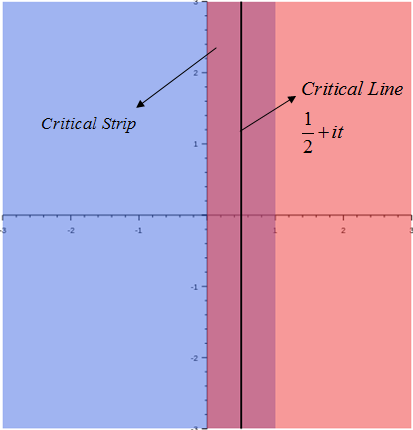
\includegraphics[width=2.0in]{critical-strip}
    \caption{Critical Strip and Line}
\end{wrapfigure}

However, the non-trivial zeros of the zeta function can be found when the real part of the function’s input is between 0 and 1 (called the critical region). This is a fact that has been proven by Riemann in his paper, and he even proved that there are an infinite amount of non-trivial zeros in the critical region. But Riemann went further than this, he hypothesised that the non-trivial zeros do not only occur when the real part of the input is between 0 and 1; but they all occur in the middle of the critical region when the real part of the input is exactly ½. The Riemann Hypothesis states that ‘the real part of every nontrivial zero of the Riemann zeta function is ½’. This is the fundamental part of the Riemann Hypothesis, and although it is widely considered to be true, this conjecture has never actually been proven with conclusive evidence, and that is why these are considered to be non-trivial zeros.


\subsubsection{The Importance of the Riemann Hypothesis}
The Riemann Hypothesis and the  Riemann Zeta Function have many extraordinary uses. From calculating prime numbers to uses in Quantum Physics, and even cryptography with the RSA algorithm. This is due to the fact that the Zeta function is deeply connected to the prime numbers.

One of the main reasons why the Riemann Hypothesis is significant is because there have been many conjectures and theories that assume the Riemann hypothesis to be true. So if the Riemann hypothesis was proven, this would also prove countless other theories.
Some of these theories include :
\begin{itemize}
    \item The weak Goldbach conjecture - stating that all integers greater than 5 are the sum of three primes
    \item Mills’ constants - numbers that allow you to generate prime numbers
    \item The theory that there will always be at least one prime between consecutive cubes
    \item The theory that there is a maximum bound between consecutive prime numbers
\end{itemize}
All of these theories are, in some way, related to the prime numbers. There is an important reason for this which I’ll cover in a later section.

If the Riemann Hypothesis was proven to be true, there would be profound effects in fields such as cryptography. In public-key cryptosystems, like RSA, public keys are created using prime numbers. If someone wanted to try and decode information without knowing what the prime numbers were that created the key, they would have to try and guess what the prime numbers were. What keeps these algorithms secure is the fact that it can take a long time to calculate the prime numbers, especially some of the larger ones. In fact, the largest prime number discovered has over 23 million digits. However, if the Riemann hypothesis were true, then people would be able to calculate the prime numbers much quicker than before. This would make many of the current cryptography algorithms obsolete.

The Riemann Hypothesis does not just influence mathematics and cryptography, it also has great importance in quantum physics. It was discovered in 1996 that the arrangement of the zeta zeros exhibits the same statistical pattern as the spectra of energy levels (that is the possible values of energy of a quantum system) in quantum chaotic systems. Furthermore, it was conjectured in 1999 by Michael Berry and Jonathan Keating, that there will exist a quantum system, where the energy levels will correspond exactly to the non-trivial zeros of the Riemann Zeta Function. If this conjecture is true, it would prove the Riemann Hypothesis.

\subsubsection{Complex Numbers and Key Operations}
Complex numbers play a key part in the Riemann Hypothesis. When Riemann created the Riemann Zeta Function, he allowed the inputs and outputs to be complex numbers, through his ideas of analytic continuation. It is therefore important to know what complex numbers are, and how to do arithmetic with them.

To first understand complex numbers (denoted by the symbol $\mathbb{C}$), it is necessary to be familiar with the idea of imaginary numbers. There is no real number whose square root is a negative number, so mathematicians decided to invent numbers for this. It is denoted by the symbol i, for the imaginary unit.

Where: $$i \equiv \sqrt{-1}$$
And thus: $$i^2 \equiv -1$$
You can multiply the imaginary unit($i$) by any real number to create an imaginary number. For example:
$$3i$$
$$2i$$
Which are both imaginary numbers.
By combining both real numbers and imaginary numbers, you can create complex numbers.
For example:
$$2+3i$$
Where the real part of the number is $2$, and the imaginary part is $3i$.
$$4-7i$$
Where the real part of the number is $4$, and the imaginary part is $-7i$.
We often represent real numbers on a number line, however, this is impossible to do with complex numbers. Instead, one way to understand them is through a two-dimensional graph, or to give it its formal name, the complex plane. On the complex plane, there are two axes, a real axis and an imaginary axis. Any complex number can be plotted on the complex plane. We can think of a complex number as a set of coordinates that tell us where the number lies on the complex plane, with the real part being the x coordinate and the imaginary part being the y coordinate.

So if we wanted to plot the point $2+3i$ on the complex plane, it would look as follows:

% \clearpage
\begin{figure}[ht]
    \centering
    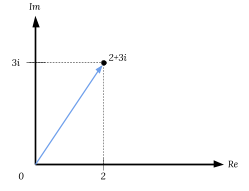
\includegraphics[scale=1]{argand diagram 23i}
    \caption{Argand Diagram of $2+3i$}
\end{figure}

This type of diagram is known as an Argand Diagram. And as you can see, we have plotted the point $2+3i$ at the coordinates $(2, 3)$ on the complex plane.

We can also do arithmetic with complex numbers - be that addition, subtraction, multiplication, division or exponentiation.

The sum of two complex numbers is the sum of both of the real parts of the numbers, plus the sum of the two complex parts of the numbers.
$$(3+2i) + (1+3i)$$
$$= (3+1) + (2i+3i)$$
$$= 4 + 5i$$

Subtraction is also done using a similar method.

$$(3+2i)-(1+3i)$$
$$=(3+2i) + (-1-3i)$$
$$=(3-1)+(2i-3i)$$
$$=2-i$$

To multiply two complex numbers, it is equivalent to expanding out two binomial brackets where:

$$(a+b)(c+d)$$
$$= ac + ad + bc + bd$$

\clearpage
So with two complex numbers this would look like:

$$(3+i)(2+2i)$$
$$= 6 + 6i + 2i + 2i^2$$
$$= 6 + 8i + 2i^2$$

We can then use the identity $i^2 \equiv -1$ to simplify this expression, so that:

$$= 6+8i + 2(-1)$$
$$= 4 + 8i$$

But we can speed up this method by using the rule $(a+bi)(c+di) = (ac-bd)+(ad + bc)i$
For example:
$$(3+i)(2+2i)$$
$$= (3\times2 - 1\times2) + (3\times2 + 1\times2)i$$
$$= 4+8i$$
We can derive this rule, to prove that it works for all complex numbers:
% \begin{align*}
    $$RTP: (a+bi)(c+di) = (ac-bd)+(ad+bc)i$$
    $$LHS =  (a+bi)(c+d$$
    Distributing Terms:
    $$=ac + adi + bci + bdi^2$$
    Using $i^2=-1$:
    $$=ac + adi + bci - bd$$
    Then rearranging:
    $$= ac-bd + adi + bci $$
    $$= (ac-bd)+(ad+bc)i$$
    $$= RHS$$
    $$\text{    }Q.E.D$$
% \end{align*}

To divide two complex numbers, we create a fraction and then rationalise the denominator, by using the identity $(a+b)(a-b)  a^2-b^2$ where $a, b \in \mathbb{C}$ (meaning that a and b are both complex numbers)
For example:
\begin{align*}
    (3-i) &\div (2-2i)\\
    &=\frac{3-i}{2-2i}
    \intertext{We can then rationalise the denominator by multiplying the numerator and denominator of the fraction by $(2+2i)$. This does not change the value of the expression but does allow for it to be simplified.}
    &=\frac{3-i}{2-2i} \cdot \frac{2+2i}{2+2i}\\
    &=\frac{(3-i)(2+2i)}{(2-2i)(2+2i)}\\
    \intertext{We can then distribute terms in the numerator and denominator, using the aforementioned multiplication rule:}
    &=\frac{(6+2)+(6-2)i}{4-4i^2}\\
    &=\frac{8+4i}{4-4i^2}\\
    &=\frac{8+4i}{4-(-4)}\\
    &=\frac{8+4i}{8}\\
    &=1-\frac{1}{2}i\\
\end{align*}

There are also some functions that we can use on complex numbers to talk about the real and imaginary parts separately.
The $\Re(z)$ function (also defined as $Re(z)$), outputs the real part of the complex variable $z$. So for example:

\begin{align*}
    \intertext{If we let} z = a+ bi\\
    \intertext{Then} \Re(z) = a
\end{align*}

Similarly, the $\Im(z)$function (also defined as $Im(z)$) outputs the imaginary part of of the complex variable $z$.
For example:

\begin{align*}
    \intertext{If we let} z = a+ bi\\
    \intertext{Then} \Im(z) = b
\end{align*}

Although these functions have limited use in equations and mathematical usage, they prove very handy when needing to discuss complex variables. It is also very useful when computing functions, to be able to split up complex numbers into their real and imaginary parts.

We can also express imaginary numbers using the trigonometric functions, sine and cosine.

Where we have the complex number such that:

\begin{align*}
    z &= a+ bi\\
    \intertext{It can be expressed such that:}
    z &= r \cdot cis(\phi)\\
    \intertext{Where:}
    cis(\phi) &= cos(\phi) + i \cdot sin(\phi)\\
    r =|z| &= \sqrt{a^2+b^2}\\
    \phi =arg(z)&= arctan\left(\frac{b}{a}\right)\\
\end{align*}

This is known as the polar form of the complex number.

We can use this form to easily calculate the value when we raise a complex number to a real power, using De Moivre’s Theorem.
De Moivre’s theorem states that for a complex number in the form


\begin{align*}
    z &= r(cos ( \phi) + i sin ( \phi))\\
    \intertext{If we raise $z$ to the power $n$ then:}
    z^n &= (r(cos(\phi) + i sin(\phi)))^n\\
    &= r^n (cos(n\phi) + i sin(n\phi))
    \intertext{Which is true for}
    &r, \phi, n \in \mathbb{R}, z \in \mathbb{C}
\end{align*}

Which means that this formula does not work when we are raising any number to a complex power.

Say we have two complex numbers $z$ and $w$  and they are of the form $a+bi$. Such that $z=a+bi$ and $w=c+di$.To calculate $z^w$, the process is best split down into multiple steps.

First we calculate $\rho$ and $\theta$, where $\rho$ is the modulus of $z$ and $\theta$ the argument of $z$
$$\rho = \sqrt{a^2 + b^2}$$
$$\theta = \arctan{\frac{b}{a}}$$
Then using these values, we can say that:
$$z^w = \rho^c e^{-d\theta}(\cos(d \ln \rho + c\theta) + i \sin(d \ln \rho + c\theta))$$
Which is true for
$$z, w \in \mathbb{C}$$


\subsubsection{The Riemann Zeta Function}

Previously I have mentioned multiple functions that play a key role in the Riemann Hypothesis, but now I aim to address and examine these functions in detail.

When discussing the Riemann Zeta Function the complex variable $s$ is traditionally used where $s =\sigma  + it$.

The Riemann Zeta Functions is defined as $\zeta(s)$ where:

\begin{align*}
    \zeta(s) &= \sum_{n=1}^{\infty} \frac{1}{n^s}\\
    &= \frac{1}{1^s} + \frac{1}{2^s} + \frac{1}{3^s} + \frac{1}{4^s} + \dots
\end{align*}

This was the equation that Leonhard Euler first introduced and studied, but it was Bernhard Riemann who defined this function for not just all of the real numbers, but all of the complex numbers. Riemann did this through the method of analytic continuation to expand the domain of the function. But by doing it he had to create a new function that would work for all possible input values. He produced what is known as Riemann's Functional Equation:

$$\zeta(s) = 2^s\pi^{s-1}sin\left(\frac{\pi s}{2}\right)\Gamma(1-s)\zeta(1-s) $$
Where $\Gamma(n)$ is the gamma function, such that:

$$\Gamma(n) = \int_{0}^{\infty}n^{s-1}e^{-n} \mathrm{d}n$$

From Riemann's Functional Equation, we can now see why the trivial zeros occur at even negative integers for $s$. This is all due to the sine function. If we let $s = -2n$ for $n \in \mathbb{N}$, (a negative even integer) then the functional equation becomes:

\begin{align*}
    \zeta(-2n) &= 2^{-2n}\pi^{-2n-1}sin\left(\frac{\pi(-2n)}{2}\right)\Gamma(1-(-2n))\zeta(1-(-2n))\\
    \Rightarrow \zeta(-2n) &= -2^{-2n}\pi^{-(2n+1)}sin(n \pi)\Gamma(2n+1)\zeta(2n+1)
\end{align*}
Now we can see that the functional equation includes a factor of $sin(n)$, but due to the nature of the sine function: $sin(n) = 0$ for $n \in  \mathbb{Z}$.  As shown in this diagram of the function $y = sin(x)$:

\clearpage

\begin{figure}[ht]
    \centering
    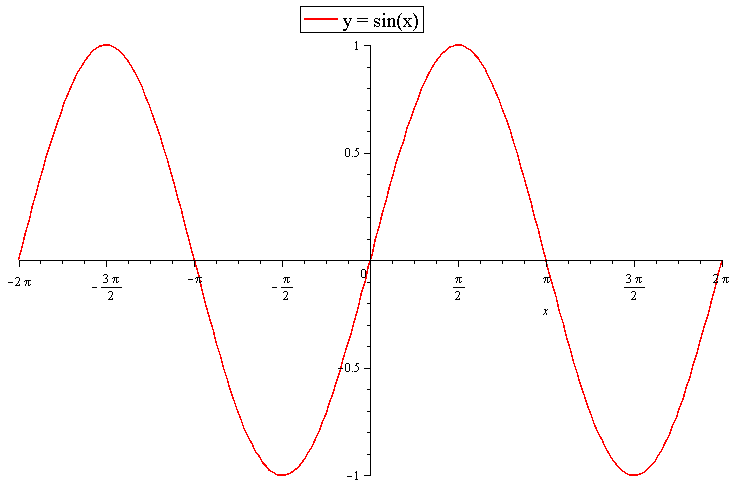
\includegraphics[scale=0.3]{sinx-graph}
    \caption{$y=sin x$}
\end{figure}

And when the sine factor of the functional equation evaluates to zero, this causes the entire function to evaluate to zero, due to the fact that anything multiplied by zero, is zero. This suggests that when s is an even integer, the zeta function evaluates to zero. But then comes the question, why does the zeta function only have zeros at the negative even integers, but not the positive ones? Well, this is because of the gamma function ($\Gamma$).  The factor $\Gamma(1-s)$ in the functional equation has simple poles at positive integers, or in other words, when $s \in \mathbb{N}, \Gamma(1-s)$ is undefined. So for $s \in \mathbb{N}$, the sine function would evaluate to 0, but the gamma function would evaluate to an undefined value. These values cancel each other out, which means that the equation does not necessarily evaluate to $0$ if  $s \in \mathbb{N}$. This is why the trivial zeros are only found at negative even integers.

However, although Riemann’s Functional Equation has significant importance; it is long, complex, and would be hard to compute; mainly due to the fact that it is recursive, with the $\zeta(1-s)$ factor. Luckily, there are other equations that we can use to compute the Zeta function more efficiently.
An example of this is by using the Dirichlet eta function, denoted by $\eta(n)$, such that:


\begin{align*}
    \eta(s) &= \sum_{n=1}^{\infty}\frac{(-1)^{n-1}}{n^s}\\
    \intertext{This function is also known as the alternating zeta function. It has the special property that:}
    \eta(s) &= (1-2^{1-s})\cdot\zeta(s)\\
    \intertext{We can now do arithmetic and rearranging of this function so that we can use it to compute $\zeta(s)$.}
    \intertext{So rearranging for $\zeta(s)$:}
    \zeta(s)&=\frac{1}{1-2^{1-s}}\cdot \eta(s)
\end{align*}


\begin{align*}
    \intertext{Now, if we let $\phi_n = log(n)$, where $log(n)$ is the natural logarithm of $n$, then:}
    n^{it} &= e^{log\left(n^{it}\right)}\\
    &=e^{it\phi_n}\\
    &= cos(t \cdot \phi_n) + i sin(t \cdot \phi_n)
\end{align*}
Then if we express $\zeta(s)$ using $\eta(s)$ in its summation form, and split the variable $s$ into $\sigma+ it$, we derive that:

$$\zeta(\sigma + it) = \frac{2^{it}}{2^{it}-2^{1-\sigma}} \cdot \sum_{n=1}^{\infty} \frac{(-1)^{n-1}}{n^\sigma} \cdot \left[ cos(t\phi_n) -i sin(t\phi_n) \right]$$

Now, this equation is very long and complex, but it seems to be relatively simple to compute.
However, due to the fact that the Dirichlet eta function is only defined for values where the real part of sis greater than one, it means that this form of the zeta function is only defined when $\Re(s) > 0$.

Similarly, we can manipulate the earlier function to find it in another form that will be easy to compute as part of a program.
\begin{align*}
    \intertext{If we take the equation from earlier that:}
    \zeta(s)&=\frac{1}{1-2^{1-s}}\cdot \eta(s)\\
    \intertext{And substitute in the eta function where}
    \eta(s) &= \sum_{n=1}^{\infty}\frac{(-1)^{n-1}}{n^s}\\
    \intertext{Then we can say that}
    \zeta(s) &= \frac{1}{1-2^{1-s}}\sum_{n=1}^{\infty}\frac{(-1)^{n-1}}{n^s}
    \intertext{Then, by performing analytic continuation by using Hankel Functions (essentially very complicated mathematics that is beyond the scope of this project), it can be derived that:}
    \zeta(s) = \frac{1}{1-2^{1-s}} \sum_{n=0}^{\infty} & \frac{1}{2^{n+1}} \sum_{k=0}^{n} (-1)^k \binom{n}{k} (k+1)^{-s}
    \intertext{Where $\binom{n}{k}$ is a binomial coefficient where:}
    \binom{n}{k} &= \frac{n!}{k!(n-k)!}
\end{align*}

Just like the previous function we derived, this does look very complicated, however for a computer, it is relatively simple to compute.

\clearpage
\subsubsection{The Riemann Hypothesis and Prime Numbers}
The Riemann Hypothesis is deeply connected to the prime numbers. If the Riemann Hypothesis was proven to be true, then the effect this would have on mathematics would be monumental.


Leonhard Euler derived a very nice equation from the Riemann Zeta Function, that involves the prime numbers. This function is known as Euler's Product Formula.

We already know that the zeta function can be defined by:

\begin{align}
    \zeta(s) &= \sum_{n=1}^{\infty}\frac{1}{n^s} \nonumber
    \intertext{Where:}
    \zeta(s) &= \frac{1}{1^s} + \frac{1}{2^s} + \frac{1}{3^s} + \frac{1}{4^s} + \frac{1}{5^s} + \dots \label{1}
    \intertext{Now if we multiply both sides by the second term: $\frac{1}{2^s}$}
    \frac{1}{2^s} \cdot \zeta(s) &= \frac{1}{2^s} + \frac{1}{4^s} + \frac{1}{6^s} + \frac{1}{8^s} + \frac{1}{10^s} + \dots \label{2}
    \intertext{Subtracting equation \ref{2} from equation \ref{1} removes all elements with a factor of 2:}
    \left(1-\frac{1}{2^s}\right) \cdot \zeta(s) &= 1 + \frac{1}{3^s} + \frac{1}{5^s} + \frac{1}{7^s} + \frac{1}{9^s} + \dots \label{3}
    \intertext{Then multiplying again by the second term, $\frac{1}{3^s}$}
    \frac{1}{3^s}\left(1-\frac{1}{2^s}\right) \zeta(s) &= \frac{1}{3^s} + \frac{1}{9^s} + \frac{1}{15^s} + \frac{1}{21^s} + \frac{1}{27^s} + \dots \label{4}
    \intertext{Subtracting equation \ref{4} from equation \ref{3} removes all elements with a factor of 3 as well as those with a factor of 2 from the right-hand side.}
    \left(1-\frac{1}{3^s}\right)\left(1-\frac{1}{2^s}\right) \zeta(s) &= \frac{1}{5^s} + \frac{1}{7^s} + \frac{1}{11^s} + \frac{1}{13^s} + \frac{1}{17^s} + \dots \nonumber
    \intertext{We can see that the right-hand side of the equation is being sieved. If we repeat this process infinitely many times by multiplying by $\frac{1}{p^s}$where $p$ is a prime number, and then subtracting. We end up with:}
    \dots \left(1-\frac{1}{11^s}\right)\left(1-\frac{1}{7^s}\right)&\left(1-\frac{1}{5^s}\right)\left(1-\frac{1}{3^s}\right)\left(1-\frac{1}{2^s}\right) \zeta(s) = 1 \nonumber
    \intertext{Then rearranging for $\zeta(s)$:} \nonumber
\end{align}
$$\zeta(s) = \frac{1}{\left(1-\frac{1}{2^s}\right)\left(1-\frac{1}{3^s}\right)\left(1-\frac{1}{5^s}\right)\left(1-\frac{1}{7^s}\right)\left(1-\frac{1}{11^s}\right) \dots} $$
We can then write this as an infinite product over all primes, $p$:
$$\zeta(s)=\prod_{p, prime} \frac{1}{1-p^{-s}}$$
This function is only defined when $\Re(s) > 0$, due to the fact that negative numbers can not be prime. Furthermore, it would be hard to compute, due to the fact that you would be required to calculate the prime numbers first.

As well as Euler's Product Formula, there are many other functions that involve the prime numbers that are all related to the zeta function.

The prime number theorem was a theorem thought of by Carl Friedrich Gauss near the end of the 18th century. This theorem describes the distribution of the prime numbers. It formalises the intuitive idea that as numbers get larger, the prime numbers are less common, by precisely quantifying the rate at which this occurs. One way this theorem was modelled was through the prime counting function (denoted $\pi(N))$. Where $\pi(N)$ gives the number of primes that are less than or equal to $N$. Given this we can say that as $N \to \infty$ then $\frac{\pi(N)}{log(N)} \to 1$, where $log(N)$ is the natural logarithm of $N$
This, therefore, means that:
$$\pi(N) \sim \frac{N}{log(N)}$$
This means we can approximate the numbers of primes less than or equal to $N$, by calculating $\frac{N}{log(N)}$
For example, if we wanted to approximate the number of primes less than $100$:
Then our approximation would be:
$$\frac{100}{log(100)} = 22$$
But the true value:
$$\pi(100) = 25$$
So there is some error in our approximation.
However, the larger the number $N$, the better our approximation for $\pi(N)$.
For example:

\begin{align*}
    \pi(1,000,000) &= 50,847,534
    \intertext{and}
    \frac{1,000,000}{log(1,000,000)} &= 48,254,942
    \intertext{where proportionally, the error is a lot s      maller}
\end{align*}
\clearpage
However, Peter Dirichlet and Carl Friedrich Gauss came up this a much better approximation for $\pi(N)$. They said that:
$$\pi(N) \sim Li(N)$$
Where $Li(N)$ is the logarithmic integral of $N$ such that:
$$Li(N) = \int_0^N \frac{1}{log(t)} \mathrm{d}t$$
Where $\log(t)$ is the natural logarithm of $t$.
Now if we wanted to use the logarithmic integral function to approximate $\pi(1,000,000)$, we get that:
$$Li(1,000,000) = 50,849,234$$
Which is only $1700$ away from the true value.


As well as the prime counting function, we also have a similar function called the prime power function (denoted by $\Pi(N)$). In the prime counting function, you would get $1$ point per prime number (less than or equal to $N$). But in the prime power function, you get $1$ point per prime $+\frac{1}{2}$ point per prime squared $+ \frac{1}{3}$ point per prime cubed and so on.
As an equation this would be:

\begin{align*}
    \Pi(N) &= \pi(N) + \frac{1}{2}\pi(N^{\frac{1}{2}}) + \frac{1}{3}\pi(N^{\frac{1}{3}}) + \dots \\
           &= \sum_{r=1}^{\lfloor log_2  N\rfloor} \pi(N^{\frac{1}{r}})
\end{align*}

But how is this related to the Riemann Hypothesis? It turns out that the prime number theorem was proved by using the Riemann Zeta Function.

Riemann came up with a function for the Zeta Function where he described it in terms of the non-trivial zeros. He stated:

$$\zeta(s) = \left(\frac{\pi^{\frac{s}{2}}}{2\left(s-1\right)\Gamma\left(\frac{s}{2}-1\right)} \right ) \cdot \prod_{\rho}\left(1-\frac{1}{\rho}\right)$$

Where $\rho$ are the non-trivial zeros of the Riemann Zeta Function.

Then through complex analysis and advanced calculus, it was derived that:
$$\Pi(x) - Li(x) = \sum_{\rho}Li(N^\rho) - log(2) + \int_{N}^{\infty} \frac{1}{t(t^2-1)log(t)} \mathrm{d}t$$

Which tells us the difference or ‘error term’ between the prime counting function, and the prime power function. The main and most influential part of this error term is the sum of the logarithmic integrals of $N^\rho$.

Because $\rho$ are the non-trivial zeros, the non-trivial zeros of the Riemann Zeta function are really controlling the size of this error term. If the Riemann Hypothesis were true and all of the non-trivial zeros lie on the critical strip, then this error term will be as small as possible.

Mathematicians were finally able to prove the prime number theorem by using the Riemann zeta function, by showing that the Riemann zeta function has no zeros on the line $\Re(s) = 1$. However, this error term is controlled by the non-trivial zeros of the Riemann zeta function, and it is still unproven whether all of the non-trivial zeros lie on the critical strip. But if the Riemann Hypothesis were true, then this error term is bounded by:

$$|\pi(N) - Li(N)| \leq c \sqrt{N} \cdot log(N)$$

Where $c$ is some constant

This means that there would also be a similar bound between consecutive prime numbers, such that:

$$p_{n+1} - p_{n} \leq c \sqrt{P_{n}} \cdot log(p_{n})$$

There are also many other consequences if the Riemann Hypothesis was proved to be true. For example, the Weak Goldbach Conjecture would also be proven true, stating that ‘All odd integers greater than 5 are the sum of three primes’. Furthermore, if the Riemann Hypothesis was true then there will always be a prime number between consecutive cubes, such that:

$$x^3 < p < (x+1)^3$$

This would mean that you could define a constant $\theta$ such that $\lfloor \theta^{3^n} \rfloor$is prime for all n. This is called a Mills’ Constant.

All of these theorems and conjectures highlight the importance of the Riemann hypothesis, and that if it was to be proven, it would lead to several major breakthroughs, not only in mathematics but quantum physics and computer science. The fact that the non-trivial zeros of the Riemann zeta function have such an importance in countless other fields just shows how influential the Riemann Hypothesis is.

\subsubsection{Visualisations of the Riemann Hypothesis}

There are numerous ways of visualising functions on graphs and plots. Throughout this next section, I will explore the different types of data visualisation techniques, as well as their positives and negatives.


The most common form of visualisation for the Riemann Hypothesis is showing how the output of the Riemann zeta function varies as you move along the critical strip. It plots the values of $\zeta(s)$ for $s = \frac{1}{2} + it$, where $it$ is some imaginary number.


% \begin{wrapfigure}{r}{2.2in}
    % \centering
    % \captionsetup{justification=centering}
    % 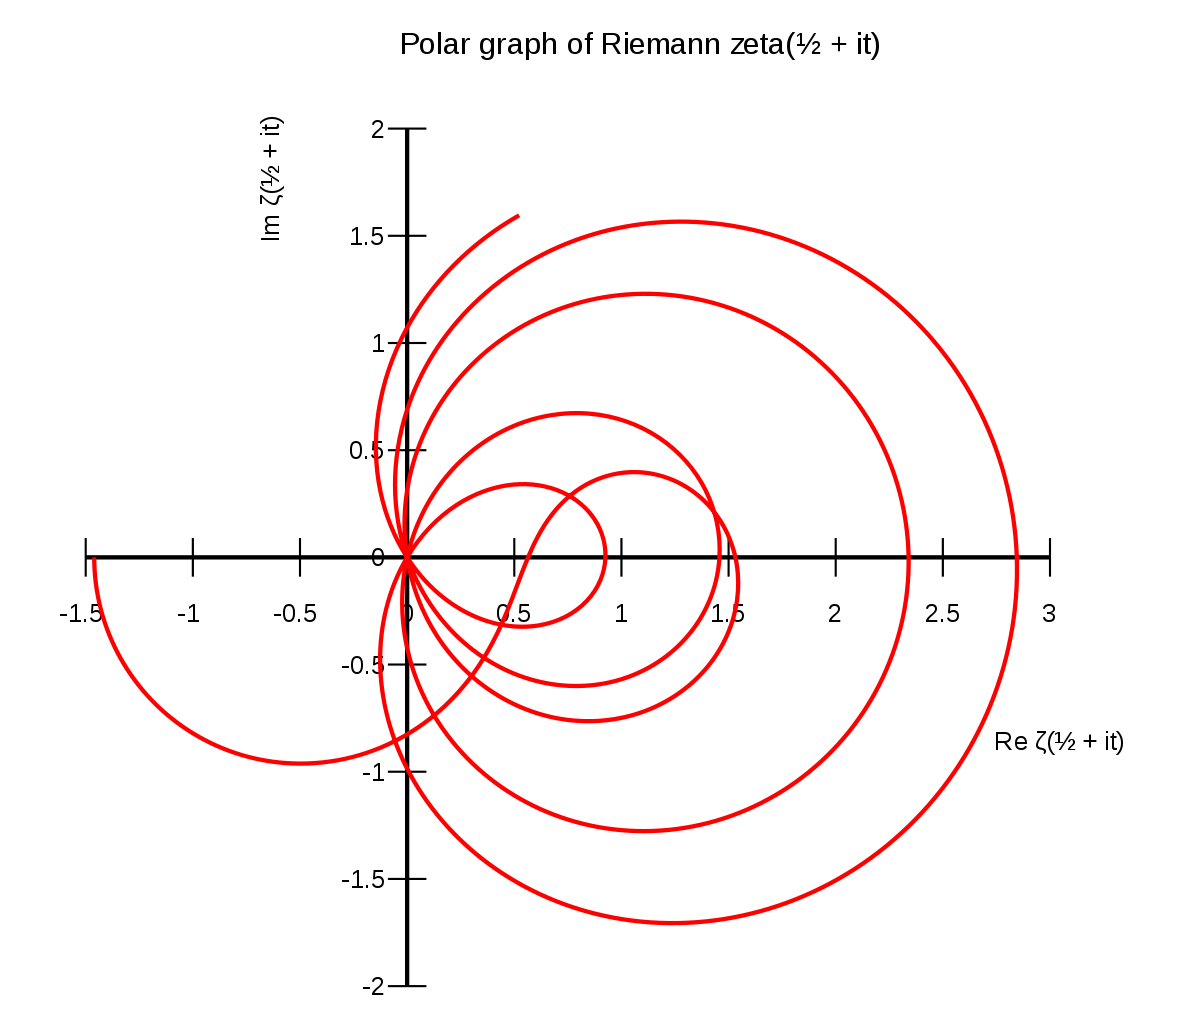
\includegraphics[width=2.0in]{Zeta-Polar-Graph}
    % \caption{\\Polar Graph of the Riemann Zeta Function}
% \end{wrapfigure}
\begin{figure}[h]
    \centering
    \captionsetup{justification=centering}
    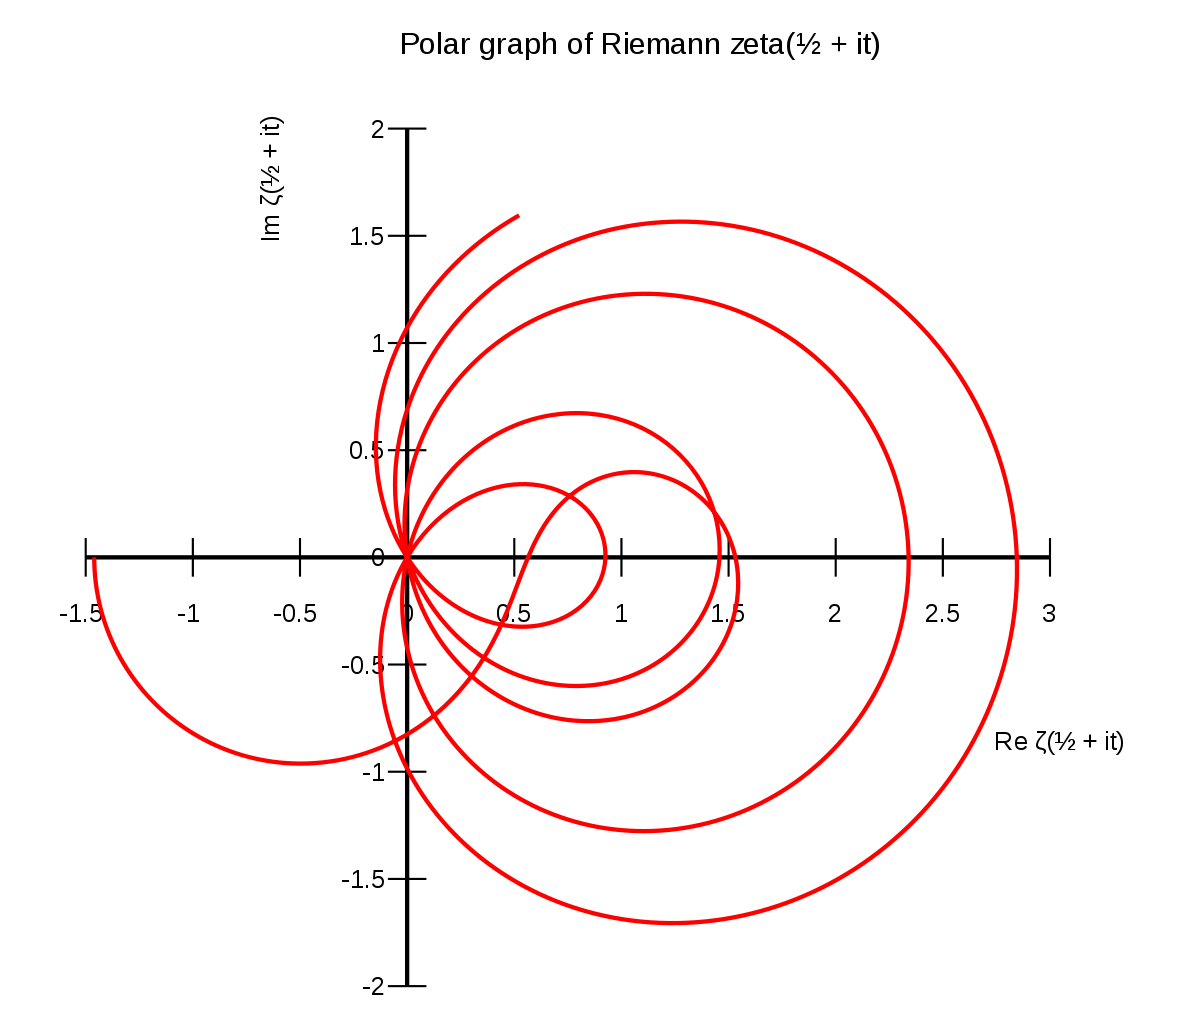
\includegraphics[width=4.0in]{Zeta-Polar-Graph}
    \caption{Polar Graph of the Riemann Zeta Function}
\end{figure}

This graph shows us how the Zeta function varies along the critical strip and allows for us to identify the non-trivial zeros of the function.

Whereas most graphs show the input to the function along a horizontal axis and the output along a vertical axis, we cannot do this with the plot of the Riemann Zeta function because we are required to use both axes to represent complex numbers on the complex plane.

Some positives about this graph are that it is simple and easy to understand. However, it would require an input value for $t$, which is not shown on the graph, for the data to have any practical use.

However, we can expand on this graph and use it to help us to create a dynamic graph. A dynamic graph is one that changes with time. To plot a dynamic graph of the Riemann Zeta function, we could plot values of $\zeta(s)$ along the critical strip so that $\zeta(s) = \frac{1}{2}+ it$. Where $t$ would be our independent variable.

However, we would be changing $t$ over time, where we would need a relationship between the time of the graph and $t$, which could be in the form of an equation.

If for example, we had it so that for every second, the value of $t$ increases by $1$, this would give us a dynamic graph that would plot the points of $\zeta(\frac{1}{2}+it)$ while the user is watching it. The graph would then be changing every second.

If we made it so that for every $0.1$ seconds then t increased by $0.1$, this would give us a much smoother plot and would be much more appealing to look at.

Although the graph at any given point in time would look the same as the previous graph, the fact that this graph is changing for the user to see makes it significantly more visually appealing. Furthermore, by changing the value of $t$ over time, it allows for the user to get a much deeper understanding of how the value of $t$ affects the values of the Riemann Zeta Function.

Another way of representing functions that involve complex numbers is through domain colouring. This technique for visualising complex functions assigns different colours to each point on the complex plane. Not only does domain colouring look very appealing and intriguing it is also very useful to be able to plot functions that require four dimensions.

\clearpage

\begin{wrapfigure}{r}{2.1in}
    \centering
    \captionsetup{justification=centering}
    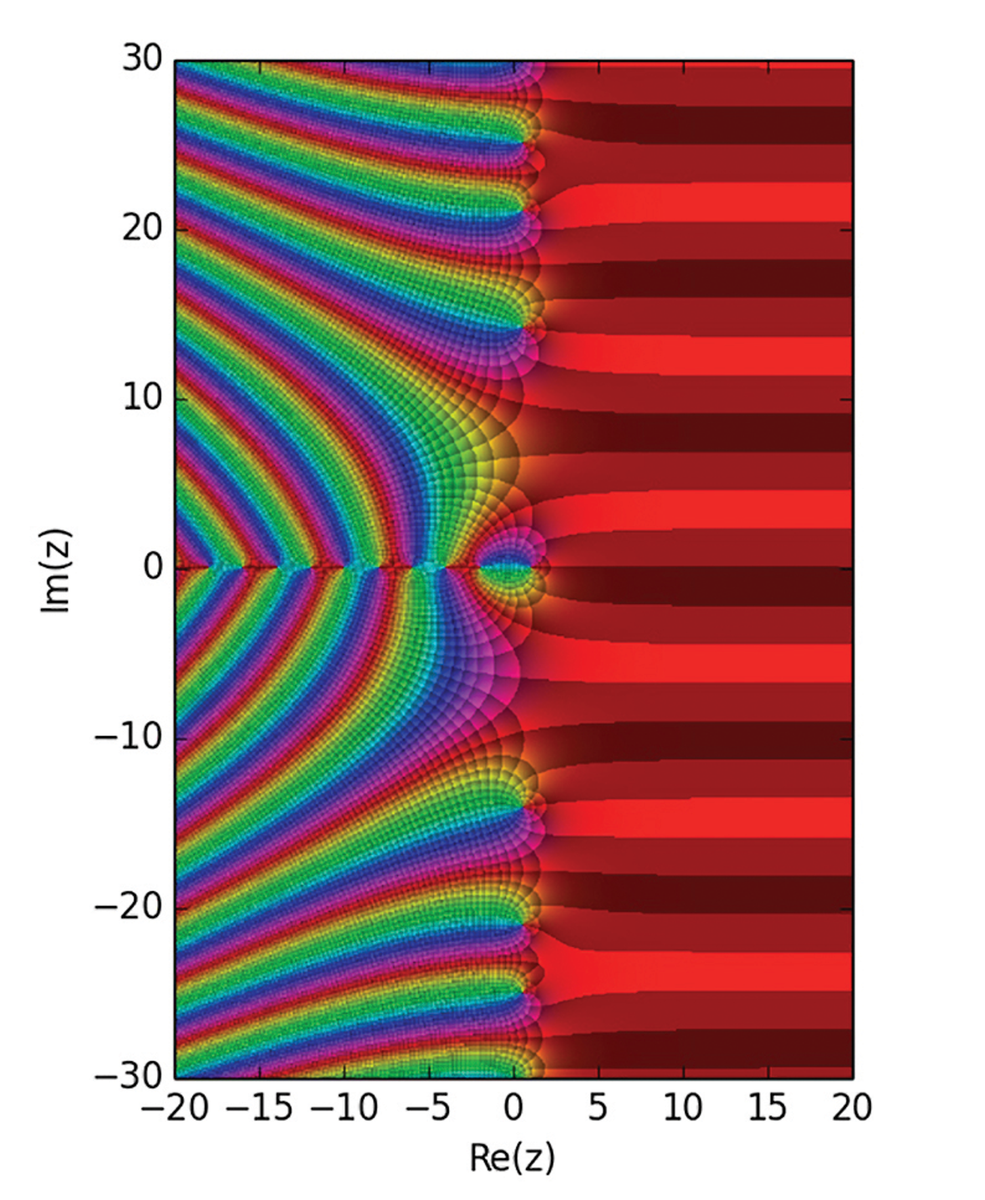
\includegraphics[width=2.0in]{domain-colouring-plot}
    \caption{The Riemann Zeta Function Plotted Using Domain Colouring}
\end{wrapfigure}

To graph a function with real inputs and outputs, two dimensions are required: one for the input and one for the output. But complex numbers are made up of two variables (the real and imaginary parts) and therefore two dimensions.

This means that in order to plot both the input and output of a complex function it requires four dimensions. The simplest way of doing this is by using the method of domain colouring.

In order to represent a function by using domain colouring, it is necessary to determine how the colours of the graph will be chosen.

There are multiple ways of doing this, but one of the most common ways is by taking the output of the function and using this to determine the hue and saturation of the colour.
\\
\\
\\
\\
For example, if we had an argand diagram for the complex number $x+iy$:

\begin{figure}[h]
    \centering
    \captionsetup{justification=centering}
    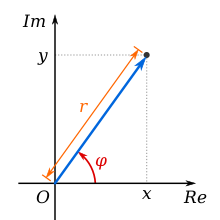
\includegraphics[scale=0.7]{argand-diagram}
    \caption{An argand diagram for the complex number $x+iy$}
\end{figure}

Then we could use the value of $\phi$ to determine the hue of the colour, and $r$ to determine the brightness of the colour.  If we did this for all outputs of a complex function, and then plotted them on a graph, then we would have a domain coloured graph.

Domain coloured graphs have multiple advantages: they look very interesting; they allow complex functions to be plotted using four dimensions; and they are useful to see the general trend of a complex function. However, these graphs are not ideal if you want to read off specific points.

Another method used to illustrate this data is through an interactive graph. An example of this could be where the user selects a complex number on the complex plane. This number is then input into the Riemann Zeta function and an animation is then displayed to show how that number gets translated by the Riemann Zeta Function. The graph would then display another data point that shows the output from the Riemann Zeta Function.

This type of graph is able to show the user how the Riemann Zeta function works and could even give insight into where the zeta zeros could be. Moreover, the interactive feature makes the graph a lot more engaging for the user.


We could also use interactive graphs to show how computers can approximate values for the Riemann Zeta function. Computers are unable to calculate the exact value of the output from the Riemann Zeta function, the reason of which I discuss later on, but it simply comes down to the fact that computers are unable to calculate the infinite series (where an infinite amount of numbers are added together) that are present in the functions. To get around this, you can compute these series to a high number that is not quite infinity, and still get a very accurate approximation.


\begin{wrapfigure}{l}{2.1in}
    \centering
    \captionsetup{justification=centering}
    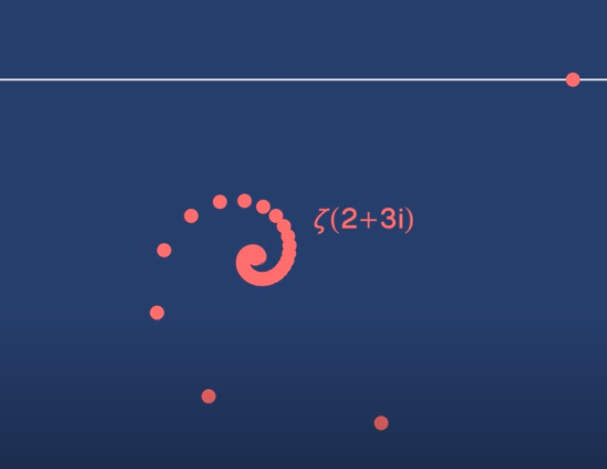
\includegraphics[width=2.0in]{zeta-approximation}
    \caption{The approximation of $\zeta(2+3i)$}
\end{wrapfigure}

As each term in the series gets calculated, the approximation gets closer and closer to the true value. We can use this fact and display it on a graph. If a user selects a point on the complex plane, we can display the approximation for $\zeta(s)$ for $1$ term, $2$ terms ... all the way up until $n$ terms (where $n$ is a high enough number so that the approximation is extremely close to the true value). The resulting graph will show a spiral of data points that converge to one point; that is the output of the zeta function. This graph allows the user to understand how the infinite series works in the zeta function, as well as how computers are able to compute the zeta function.
\\
\subsubsection{Data Storage}

As part of this program, I aim to be able to store the values of the $\zeta(s)$ for specific values of $s$. There are multiple ways to store data sets such as different file types and databases. I will be exploring these data storage methods and finding which method is best suited for my program.

The simplest way of storing data is by storing it in a text (.txt) file. These files store plain text that can be read from and written to. There is limited functionality when it comes to storing data in text files; as you can only read from and write to them. This could be used to store relatively simple and small amounts of data, but to store anything larger and more complex, text files won't be the best choice.

Another way of storing data is by using comma-separated values (CSV) files. These files consist of numerous records and fields, where each line is a record and the fields are separated by delimiters  - often commas.

\begin{wrapfigure}{l}{2.1in}
    \centering
    \captionsetup{justification=centering}
    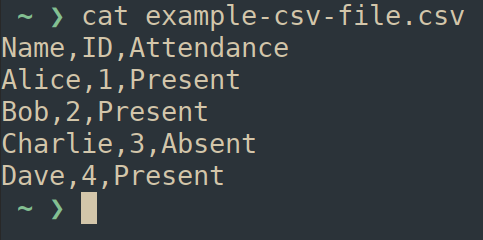
\includegraphics[width=2.0in]{example-csv-file}
    \caption{An example CSV file}
\end{wrapfigure}

This type of storage for data has a lot more functionality than using plain text files. The use of field headers allows entire fields to be read or written to with ease and data can easily be sorted, grouped, and processed. However, some downsides of using the CSV data format are that only basic data can be stored. Complex tables and configurations cannot be used with CSV files. Furthermore, there is no distinction between text and numerical values which can make processing the data difficult.
\clearpage
 Undoubtedly, one of the most efficient ways of storing large data sets is by using databases. More specifically, by using Structured Query Language (SQL).

SQL is a declarative programming language, making it very efficient to use. Databases allow for large amounts of data to be written and read very quickly.

Moreover, processing this data can be very simple with packages such as SQLite that allows SQL databases to be accessed with Python. SQL databases are efficient and can store large amounts of data, making them ideal for a project like this.

\subsubsection{Programming Languages}

There are multiple programming languages that I could - relatively easily -  use for this project, but it is important to choose a language that is suited for the task at hand. Every language has its advantages and disadvantages. Throughout this section I will evaluate various languages and whether or not they would be suitable for this project. I will then give my overall verdict on which language I wish to use.

C++ is a fairly low-level compiled programming language. Its use of classes and memory manipulation allows for an extensive range of functionality. Furthermore, with countless libraries and support, there is almost no limit to what can be done in C++. This is one of the main benefits of this language, alongside the fact that it can run incredibly fast compared to some other interpreted languages, and that it can run on almost any machine. However, the actual coding in C++ is long and tedious. Especially for a project like mine where memory management is not too much of an issue, it seems unnecessary to have to code in C++.

Javascript is also another programming language that could be used for this project. Unlike C++, Javascript is used for more high-level projects, predominantly for web applications.  Making a web app has many advantages, such as high accessibility for multiple users. However, this would require an internet connection to run, and the speed of the program would be significantly reduced compared to that of a compiled application,

Python 3 is a high-level interpreted programming language, with a wide range of libraries and packages to support it. The main advantage of Python is that the code has high readability. This allows for it to be understood by people, even if they are not familiar with the language. Although Python is an interpreted language, there are ways to compile the code into an executable file that can be run on machines that do not have the interpreter installed. As well as this, Python has wide support for user interfaces and the plotting of graphs.

Overall, I think that Python 3 will be the programming language that is most suited for my project. A web application is not what my users are looking for, so javascript would be impractical to use. The high readability and high-level features are what makes Python the optimal programming language for this project, over Javascript and C++.
\clearpage
\subsubsection{Product Research}

Throughout this section, I will be taking a look at other programs that have similar features to mine. I will talk about the advantages and disadvantages of each program and how I can incorporate some of their features into my project.

% \begin{wrapfigure}{r}{2in}
    % \centering
    % \captionsetup{justification=centering}
    % 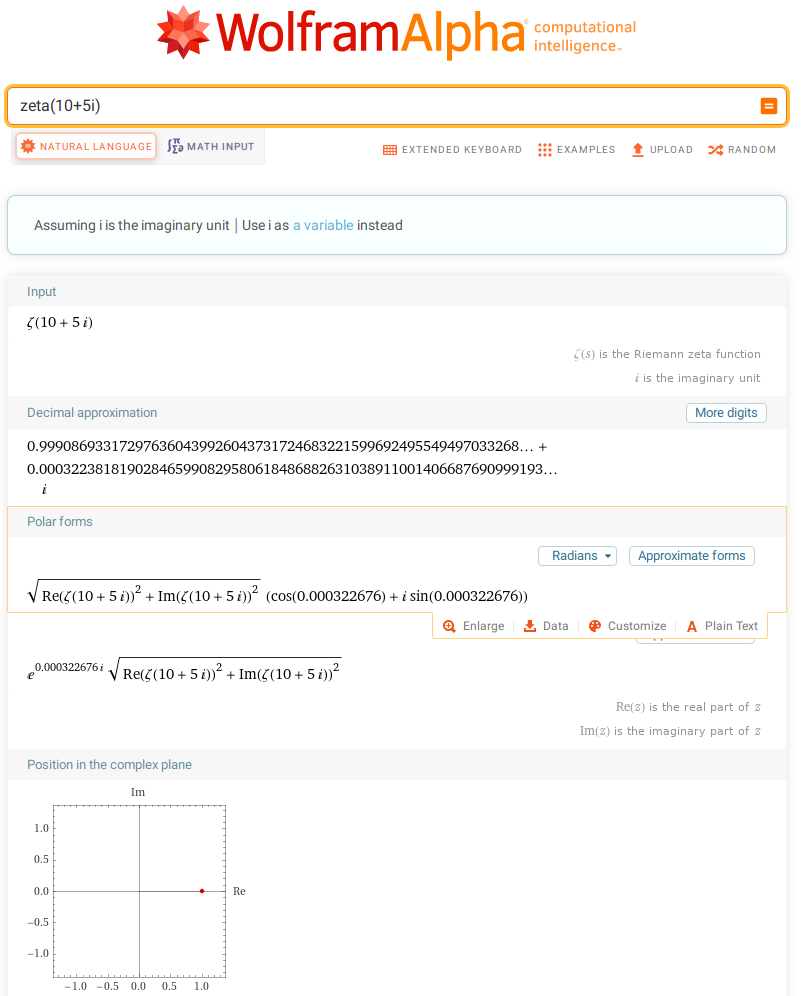
\includegraphics[width=1.9in]{wolfram-alpha}
    % \caption{Wolfram Alpha}
% \end{wrapfigure}

One of the most major programs I will look at is the web application WolframAlpha. This is a mathematical computation site, where users can input a maths query into a search bar. The answer to the query is then returned, along with information about the solution.
\begin{figure}[ht]
    \centering
    \captionsetup{justification=centering}
    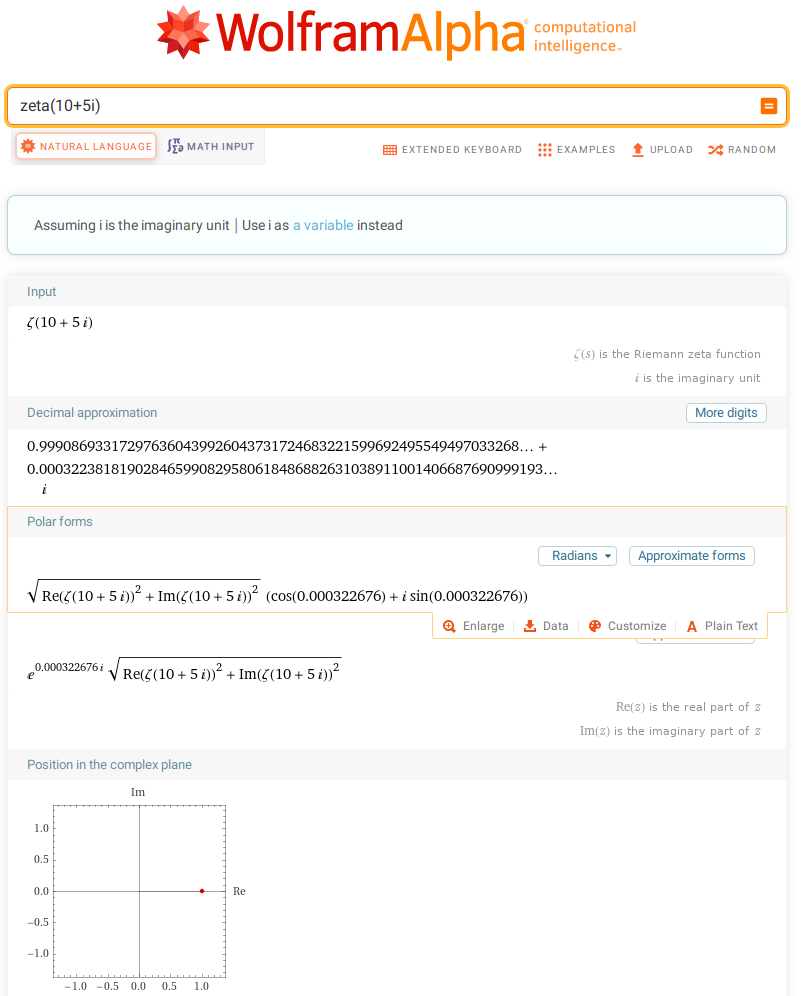
\includegraphics[width=4in]{wolfram-alpha}
    \caption{Wolfram Alpha}
\end{figure}

In this example, I input zeta(10+5i). The program then outputs a decimal approximation of the answer to my query, as well as a diagram showing the output on the complex plane. Further down the page, the program lists alternative ways that I could’ve written my input.

This application works very well for calculating specific values of the zeta function, but it does little to show the mathematics of what’s happening to calculate the answer.
\clearpage

Another web application by Wolfram Research is the Riemann Zeta Function Page on Wolfram Mathworld.

% \begin{wrapfigure}{l}{2in}
    % \centering
    % \captionsetup{justification=centering}
    % 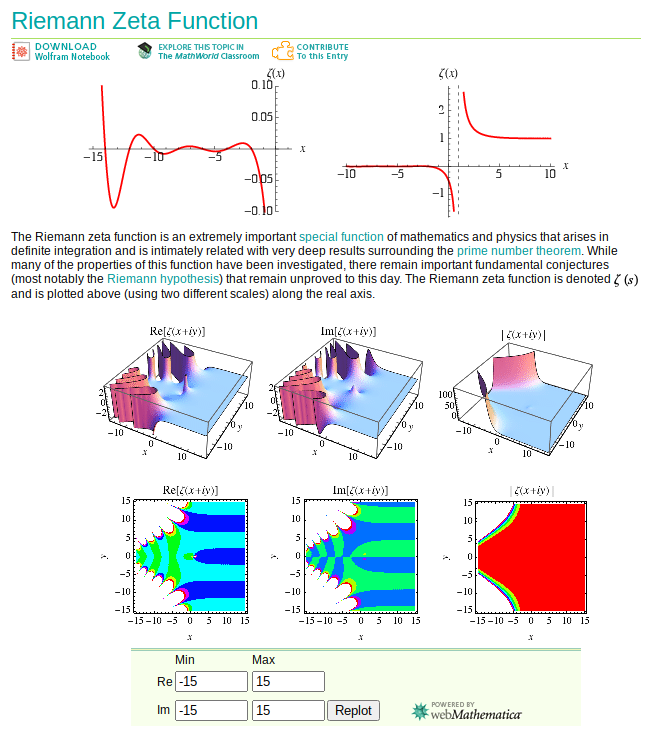
\includegraphics[width=1.9in]{wolfram-mathworld}
    % \caption{Wolfram Mathworld}
% \end{wrapfigure}
\begin{figure}[ht]
    \centering
    \captionsetup{justification=centering}
    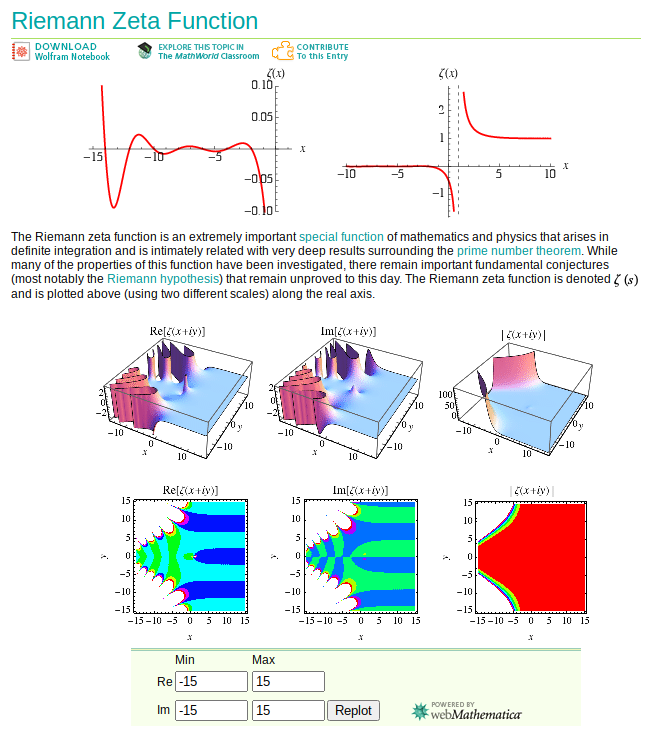
\includegraphics[width=4in]{wolfram-mathworld}
    \caption{Wolfram Mathworld}
\end{figure}

This site explains the Riemann Hypothesis in great detail, giving the user a very thorough understanding of the subject. There are also multiple three-dimensional and domain coloured graphs that plot the Riemann Zeta Function. The user is able to change the scale of the plots to see how the zeta function changes, depending on the input. The web page contains a variety of different graphs and lots of maths along with explanations as to what is going on.

However, the maths on this page is very complex and it would be unlikely that people would understand this page if they didn't have some significant background knowledge into the Riemann Zeta function, or advanced maths in general. The page is also very linear starting from top to bottom. Overall, I like the way that the graphs are presented and explained here, however, the large quantity of maths displayed can seem confusing and unrelated.

\clearpage
The next program that I will look at is Verifying The Riemann hypothesis by Aaron Meurer.

\begin{figure}[ht]
    \centering
    \captionsetup{justification=centering}
    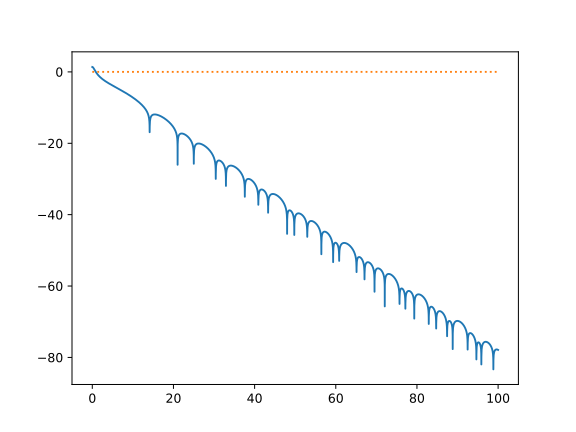
\includegraphics[width=4in]{verifying-riemann-hypothesis}
    \caption{Verifying the Riemann Hypothesis by Aaron Meurer}
\end{figure}

He creates a program that finds the non-trivial zeros of the zeta function and displays this data on some very simple and understandable graphs. I like this program a lot because it contains a lot of relevant information.

Some positives of this program are that the graphs in it are presented and explained well so that anyone could understand what is going on. The only drawback is that this isn't a very extensive program. Only 2 graphs are calculated and there isn't a user interface.

Overall this program contains some appealing and useful information and graphs but could be more refined.

To conclude the product research, there are many aspects of current programs that will be useful to include in my project, however, I can see that I will have to make mine different enough such that it is not too similar to these over programs, and ideally would contain more features.
\clearpage
\subsection{Project Objectives}
My overall aim of this project is to be able to visualise and examine the Riemann Hypothesis, to make the complicated maths more accessible and to test whether the Hypothesis actually is true. I will be doing this by completing the following key objectives.
\begin{enumerate}
    \item The program will be interactive and engaging for the user
        \begin{enumerate}
            \item There will be various questions throughout the program that the user can answer
            \item The user will be able to make notes on any of the content in the program
            \item The user will be able to choose what they do and where they go in the program, not forced along a single route
            \item The user will be able to input their own values into various functions and graphs
        \end{enumerate}
    \item The user will be able to save their progress through the program via a login system
    \begin{enumerate}
        \item The login system should allow the user to:
        \begin{enumerate}
            \item Sign in to their account
            \item Create a new account
            \item Reset their password if they want to change it
            \item Reset their password if they have forgotten it
        \end{enumerate}
        \item Multiple users will be able to make separate accounts on the system
        \item The user's data such as passwords must be saved securely
        \item The user must be able to see how they have progressed throughout the program
    \end{enumerate}
    \item The user will be given some background information about the Riemann Hypothesis such that almost anyone could feel comfortable using the program
    \begin{enumerate}
        \item The user should be able to learn the historical background of the Riemann Hypothesis
        \item The user should be able to learn what imaginary and complex numbers are
        \item The user should be able to learn what the Riemann Hypothesis states
        \item The user should be able to learn about the practical applications of the Riemann Hypothesis
    \end{enumerate}
    \item The program will allow the user to plot various graphs in order to develop their understanding of the Riemann Zeta function and allow them to learn about it
    \begin{enumerate}
        \item A polar graph of the Riemann Zeta Function
        \item A graph of the prime counting function, and other related functions used to estimate it
        \item A graph of the zeroes of the Riemann Zeta Function
        \item A visualisation of the convergence of the infinite series in the Riemann Zeta Function
    \end{enumerate}
    \item The user will be able to calculate specific values of the Riemann Zeta Function
    \begin{enumerate}
        \item A single calculator, where the user inputs a complex input and receives an output
        \item A table calculator, where the user can calculate the zeta function for a range of input values
        \item A leaderboard showing how many values of the zeta function, each user has computed
        \item The program will allow the user to store these value(s) to a database and to a csv file
    \end{enumerate}
    \item The user will be able to calculate the zeroes of the Riemann Zeta Function
    \begin{enumerate}
        \item The user will input how many zeroes they want to calculate
        \item The program will calculate these zeroes
        \item The zeroes will be displayed to the user in a table
    \end{enumerate}
    \item The user will be able to store the data that they have collected
    \begin{enumerate}
        \item The program will include a database of multiple values and zeroes of the zeta function
        \begin{enumerate}
            \item The user will be able to store values of the zeta function
            \item The user will be able to store the non-trivial zeta zeros
            \item The user program will retrieve data from the database and display its contents suitably to the user
        \end{enumerate}
    \end{enumerate}
    \item The Program will have a graphical user interface
\end{enumerate}
\clearpage
\subsection{Third-Party Input}

Throughout the following section, I will be discussing the consultation and guidance that I have received from various third parties. This section will cover the significance of third party input, who my third parties are, how and why I will be conducting my research, a transcript of the actual interviews themselves and my conclusions and takeaways from them.

\subsubsection{The Significance of Third Party Input}
Collecting third party input is vital in creating a successful project. It will allow me to assess the progress that I have made so far in my project, and check that I am heading in the right direction. Having input from various different people allows for people to view the project in different ways, each giving their own advice towards it. Third-party input and feedback is extremely important because it can help me develop and improve my project.

\subsubsection{Who are my Third Parties?}
There are benefits and drawbacks to each person you have as a third party. These depend on their relationship with me, their experience with creating projects like these and their willingness to help; just to name a few factors.

For my third parties, I am using friends who are computer science and further maths students. The benefits of this are that they have good availability, and I can talk to them regularly about the project. Furthermore, they are very supportive and encouraging. Because they are further maths and computer science students, they are also very knowledgeable about the subject area. However, the drawbacks of having friends as third parties are that they are potentially biased towards my project and could be unwilling to criticise it. It could be hard for them to tell me what is wrong, or what could be improved.

\subsubsection{How and Why I will be Conducting My Research}
I will be conducting my third party research by conducting interviews with my third parties. By creating a list of questions, I am able to ask specific questions that are useful to me. I have tailored the questions such that I can use the answers to help improve my project.

The interviews start with me asking questions to the third parties and taking answers from them. At the end of the interview, the third parties have an opportunity to ask me any questions that they have about the project.

\subsubsection{Interview Transcript - Student 1}

\textbf{Question: What will an end-user be able to gain from using this project, how would it be helpful to them?}

Answer: As a maths and further maths student, I want to be able to extend my knowledge of these subjects. This project looks like a good resource that will allow someone to understand the Riemann Hypothesis.

\textbf{Question: What features could be implemented into the project such that the end-users can accomplish what was mentioned in the previous question?}

Answer: It would be very beneficial to the user to have an explanation of the theory behind the Riemann Hypothesis at the beginning of the program. I'd like to do a couple of example steps, so I can try and understand the program before I start using it. You could have an example graph and pause the graphing animation and explain at each point what is happening. As well as this, I would like the program to be interactive so that I can really control what is happening.

\textbf{Question: How accessible would this project be for someone with little or no knowledge of the subject area?}

Answer: Due to the nature of the project, it is not extremely accessible. However, for someone with an interest in mathematics, they may be more willing to research around the topic to gain an understanding

\textbf{Question: What could be done such that people who have less experience with the subject matter are still able to understand the program? How could it still be relevant to them?}

Answer: For people with less experience, you could add some of the background information and story about the Riemann Hypothesis and the investigation. Mention why it's so important, and how it came to be. Not just the maths but the history behind it.

\textbf{Question: Which parts of the project interest you; what would you like to research further?}

Answer: The links to cryptography interest me. The fact it’s such a modern-day feature of life, actually using the function that was theorised so long ago. I am interested in the practical applications of the Riemann Hypothesis and how it actually relates to me.

\textbf{Question: How would someone be able to use this project to extend their knowledge of this subject area?}

Answer: You would be able to use the interactive interface to manipulate and break down the theory of the hypothesis, in order to gain a deeper understanding of it

\textbf{Question: Which features of the project do you like, and why?}

Answer: Visualising is helpful for exploring the project. I like the graphs, the fact it has a visual element is very appealing. It is easier to appreciate the graphs than just looking at mathematical equations.

\textbf{Question: Which features of the project do you think could be improved?}

Answer: The accessibility to the project could be improved; in terms of the mathematics knowledge needed to understand it as well as how the program can be physically accessed and run. For example, as a downloaded piece of software or as a web application.

\textbf{Question: Have you used any similar programs to this? What were they like?}

Answer: A program that seems similar to this that I have used is the practical investigation software Focus eLearning. I used this to carry out practical investigations and consolidate learning. I liked that it was accessible over the internet and that it gave me explanations of the theory, with a visual exploration of the theory it was trying to explain, in the form of the interactive practical experiment. However, I felt that the user interface was difficult to navigate.

\textbf{The question they asked me: How will you refine the access of the project so that everyone can use it?}

My answer: I will include a detailed description and explanation of the Riemann Hypothesis as part of the program to make sure that whatever your mathematical ability, you will still be able to use the program.

\subsubsection{Interview Transcript - Student 2}

\textbf{Question: What will an end-user be able to gain from using this project, how would it be helpful to them?}

Answer: The Riemann Hypothesis itself is used in so many areas such as in cryptography and quantum physics, talking about the practical uses of the hypothesis would be helpful for the user to gain an insight into why the hypothesis is so important.  I am interested in the practical usage of theory in computing and physics. Being able to understand the Riemann Hypothesis visually is also very helpful. Being able to graphically plot the many functions will give a deeper understanding of the project. Furthermore, being able to change the input values to the functions would help so that the user can expand their knowledge of the function

\textbf{Question: What features could be implemented into the project such that the end-users can accomplish what was mentioned in the previous question?}

Answer: It would be very good to make the graphing program interactive. This can be done by changing the function’s input values, but also being able to traverse the plot by scrolling around and zooming in and out by changing the scale. It would also be useful to have multiple graphs displayed on the same set of axes to compare values.

Following along with this interactive idea, I think that you could questions for the user to answer about the hypothesis, to help solidify their understanding of it. It could be beneficial to add sections where the user and write down their observations and any conclusions that they have drawn from the investigation.

To implement this, you could create a login system where a user creates a username and password, so that they would be able to save their progress in the program.

\textbf{Question: How accessible would this project be for someone with little or no knowledge of the subject area?}

Answer: I believe this project will be relatively accessible because it mainly involves just displaying maths functions, where it takes an input and gives an output. It's relatively easy for someone to use it without knowing the details of how it works. That is, to be able to use the program, but maybe not fully understand it. But then to get a deeper understanding of the project, it takes more in-depth knowledge.

\textbf{Question: What could be done such that people who have less experience with the subject matter are still able to understand the program? How could it still be relevant to them?}

Answer: Start off by just exploring and explaining the hypothesis, how it works and how the Riemann zeta function works. If the user wants to understand it further, you can go through the maths of how it works; explaining the Riemann Hypothesis in detail. You could graph the individual mathematical functions in order to break down the problem for the user to understand.  You can use 3D graphs and different ways of representing the data. This could make it easier for the user to understand.

\textbf{Question: Which parts of the project interest you; what would you like to research further?}

Answer: I am very interested in the cryptography application of the Riemann hypothesis. You could showcase as part of this project, a cryptography program that utilises the Riemann hypothesis in a practical way.

\textbf{Question: How would someone be able to use this project to extend their knowledge of this subject area?}

Answer: By utilising the multiple mathematical functions of the Riemann Hypothesis, the user could investigate how changing the input values changes the output. This will help the user learn about the individual functions and their use cases. When combining these functions together, it is important for you to be able to show how changing one piece of data can entirely change the output of a function, especially if the functions are all linked together. You should create the program such that the users could use it to investigate the domains and ranges of the functions.

\textbf{Question: Which features of the project do you like, and why?}

Answer: I like the idea of having an introduction where you explain the practical uses of the Riemann Hypothesis, and where you can give an explanation of how to use the Riemann Hypothesis and Riemann Zeta Function in other programs such as in the RSA cryptosystem. I like how the user would be able to change and manipulate the graphs to their liking and how easy it is to compare values of separate functions. It’s also a good idea to have a  conclusion/summary to help the user fully understand the maths.

\textbf{Question: Which features of the project do you think could be improved?}

Answer: It would be good for the user to be able to draw their own custom graph functions on the same axes as the functions in the program because currently, you would not be able to compare the functions in the program to the user’s own custom functions. A drawback of the project is that the maths could be too specific and intricate for the user to gain a proper understanding of the project. It would require a lot of research to fully understand the project and to be able to make the most of it.

\textbf{Question: Have you used any similar programs to this? What were they like?}

Answer: A program like this that I have used is desmos. Desmos, a graphing software, allows you to plot many graphs on top of each other, you can easily change the axes as well as any input values. What’s bad about desmos is that it doesn’t allow you to plot in 3D, it would be nice to see this in your project. Another program similar to this is Graphing Calculator 3D.
This allows you to do what desmos does, but it plots in 3D. However, its downsides are that It’s not very user friendly and the menus are not easy to navigate, so it can be hard for new users to understand how the software works.

\textbf{Questions asked to me:}

\textbf{Question: What are the necessary system requirements?}

Answer: The necessary system requirements for this program are not very high. The functions are very memory and time efficient so the specifications of the systems that the program is run on should not be an issue.

\textbf{Question: What would help the software be more useful to the user?}

Answer: If that program gave an in-depth explanation of the Riemann Hypothesis, the user can gain a full understanding of what is going on. Furthermore, examples of the practical applications of the Riemann Hypothesis, make the program more relevant to the user and makes this program practical use instead of just being theory.

\textbf{Question: With such complicated functions, how long would it take to compute them?}

Answer: The functions I have written are very memory and time-efficient, it will not take an extensive amount of time to compute the required mathematical functions.

\textbf{Question: To what degree of accuracy will the functions be plotted?}

Answer: The user will have an option where they can increase or decrease the accuracy of the functions. However, this will come with the disadvantage that it will take longer to compute.

\subsubsection{Interview Conclusion}
There are multiple improvement points from these interviews that I have used to help develop the plan for my project.

One of my main improvement points is with the design and layout of the project. The program will have 3 main sections: the introduction, the investigation, and the summary.

The introduction section will let the user be able to read and learn about the Riemann Hypothesis, so they can get an understanding of it, before using the main program. This introduction aims at making the program more accessible to people, even if they have less experience with maths. It will also allow people to explore the Riemann Hypothesis’ links to cryptography and other practical applications so that they can explore it in more detail.

After the introduction will be the actual practical investigation, this is where the user can plot graphs and really investigate the Riemann Hypothesis. They will be able to plot multiple graphs on the same axes in order to be able to compare values. The user will also be able to easily change the input values to many of these graphs so that they can investigate how this changes the outputs.

The final part of the program will be a summary; showcasing the results from the investigation that they have conducted, and detailing some of the key mathematics behind the investigation.

Breaking down the project into these three sections will allow for the User Interface of the program to be simple, such that the user can access all of the relevant parts of the program easily.

Another part of the project spoken about in these interviews was a login system to help save a user's progress through the program. There would be multiple points in the program where the user can answer questions about the hypothesis to check understanding, or for the user to just write down any conclusions that they make about the investigation and the Riemann Hypothesis. Thus, creating a login system would allow a user to save their progress in the program, and any of their answers and data can be stored in a database.
\clearpage
\subsection{Modelling the Problem}
In this section, I will report any modelling of my project that will inform the design stage. I will be covering how to compute certain mathematical functions and also try some prototypes for what the project will look like.

\subsubsection{Prototypes}

Throughout this next section, I will be prototyping some mathematical functions in Python that will allow me to compute the Zeta Function. I will then test each of the functions to make sure that they work as expected.

The majority of functions that I intend to use involve an infinite sum, which is something that we are unable to compute because it would be impossible to add up an infinite amount of numbers. Therefore we must approximate the value of the function by calculating it for a certain number of terms. For example, when calculating the zeta function where:

$$\zeta(s) = \sum_{n=1}^{\infty} n^{-s}$$

We can approximate the value but calculating the sum to such a high number, that the error difference is not significant. If we want to approximate the zeta function, we could compute:

$$\zeta(s) = \sum_{n=1}^{1 \times 10^6} n^{-s}$$

Which would not give us the exact value, but one close enough that we can still use.

First of all, is a function that computes the zeta function by its definition. $\zeta(s) = \sum_{n=1}^{\infty} n^{-s}$. This function is defined for $\Re(s) > 1$ and could look as follows in Python 3:

\begin{lstlisting}
# calculates zeta(s) for any complex number where Re(s) > 1
# where \zeta(s)=\sum _{n=0}^{\infty }\frac{1}{n^s}
def zeta(s: complex) -> complex:
    TERMS = 5 * 10**3 # the number of terms that we wish to compute.
    result = 0
    # computes an approximation for the infinite sum
    for n in range(1, TERMS+1):
        result += 1/(n**s)
    # output the final result
    return result
\end{lstlisting}

First, we define the function \textit{zeta(s)}, where \textit{s} is a complex variable. Then the constant \textit{TERMS} is defined then defined to be a large integer. This number determines how many times we calculate $\frac{1}{n^s}$ and therefore determines how accurate our approximation will be. Then in the for loop, we calculate $n^{-s}$ for \textit{TERMS} many times and sum it to our result. We then return the complex variable res in order to output from the function.

Here we can test the function to show if and when it works as expected, and also how accurate it is to the true value.
\clearpage
\begin{table}[ht]
    \centering
    \begin{tabular}{|c|c|c|c|c|c|c|}
    \hline
    \textbf{No.} & \textbf{Type} & \textbf{Input} & \textbf{Expected Output} & \textbf{Output} & \textbf{Result}\\
    \hline
    \hline
    1 & Invalid & -1 & ValueError & 12502500.0 & Fail\\
    \hline
    \multicolumn{2}{|c|}{Comment} & \multicolumn{4}{|c|}{This output is neither the output we were expecting}\\
    \multicolumn{2}{|c|}{} & \multicolumn{4}{|c|}{nor the correct output of $\zeta(-1)$. I will need to fix}\\
    \multicolumn{2}{|c|}{} & \multicolumn{4}{|c|}{this by validating the input to check that it is}\\
    \multicolumn{2}{|c|}{} & \multicolumn{4}{|c|}{within the defined range of the function}\\
    \hline
    \hline
    2 & Invalid & 0 & ValueError & 5000.0 & Fail\\
    \hline
    \multicolumn{2}{|c|}{Comment} & \multicolumn{4}{|c|}{This is the same situation as test number 1}\\
    \hline
    \hline
    3 & Boundary & 1 & ValueError & 9.095 & Fail\\
    \hline
    \multicolumn{2}{|c|}{Comment} & \multicolumn{4}{|c|}{This is the same situation as the previous tests}\\
    \hline
    \hline
    4 & Valid & 1.5 & 2.61 & 2.584 & Fail\\
    \hline
    \multicolumn{2}{|c|}{Comment} & \multicolumn{4}{|c|}{Although this gives an output that is close to the}\\
    \multicolumn{2}{|c|}{} & \multicolumn{4}{|c|}{expected output, it is not accurate enough. I need}\\
    \multicolumn{2}{|c|}{} & \multicolumn{4}{|c|}{to increase the number of terms in order to get a}\\
    \multicolumn{2}{|c|}{} & \multicolumn{4}{|c|}{more accurate output}\\
    \hline
    \hline
    5 & Valid & $5$ & $1.025$ & $1.025$ & Pass\\
      & & $+10i$ & $-0.015i$ & $-0.015i$  & \\
    \hline
    \multicolumn{2}{|c|}{Comment} & \multicolumn{4}{|c|}{This test gives a value that is extremely close to the}\\
    \multicolumn{2}{|c|}{} & \multicolumn{4}{|c|}{true value. It see,s that out approximation becomes}\\
    \multicolumn{2}{|c|}{} & \multicolumn{4}{|c|}{more accurate as the input value increases.}\\
    \hline
    \end{tabular}
\end{table}
Based on the testing, I have made some adjustments to the function as seen here:

\begin{lstlisting}
# calculates zeta(s) for any complex number where Re(s) > 1
# where \zeta(s)=\sum _{n=0}^{\infty }\frac{1}{n^s}
def zeta(s: complex) -> complex:
    # validate that Re(s) > 1
    if not s.real > 1:
        raise ValueError('Real part of input must be greater than 1')
    TERMS = 1 * 10**6 # the number of terms that we wish to compute.
    result = 0
    # computes an approximation for the infinite sum
    for n in range(1, TERMS+1):
        result += 1/(n**s)
    # output the final result
    return result
\end{lstlisting}

The first change I made was validating the input. Now if the real part of the input is less than $1$, then a \textit{ValueError} is raised. Secondly, I have increased the number of \textit{TERMS} that are computed in order to make the program more accurate. Although this does make the program take more time, the time difference is hardly noticeable.

Now here are the testing results for the improved function:
\clearpage

\begin{table}[ht]
    \centering
    \begin{tabular}{|c|c|c|c|c|c|c|}
    \hline
    \textbf{No.} & \textbf{Type} & \textbf{Input} & \textbf{Expected Output} & \textbf{Output} & \textbf{Result}\\
    \hline
    \hline
    1 & Invalid & -1 & ValueError & ValueError & Pass\\
    \hline
    \multicolumn{2}{|c|}{Comment} & \multicolumn{4}{|c|}{This works as expected; the error is raised}\\
    \hline
    \hline
    2 & Invalid & 0 & ValueError & ValueError & Pass\\
    \hline
    \multicolumn{2}{|c|}{Comment} & \multicolumn{4}{|c|}{This works as expected; the error is raised}\\
    \hline
    \hline
    3 & Boundary & 1 & ValueError & ValueError & Pass\\
    \hline
    \multicolumn{2}{|c|}{Comment} & \multicolumn{4}{|c|}{This works as expected; the error is raised}\\
    \hline
    \hline
    4 & Valid & 1.5 & 2.61 & 2.61 & Pass\\
    \hline
    \multicolumn{2}{|c|}{Comment} & \multicolumn{4}{|c|}{This functions output is very close to the true value}\\
    \hline
    \hline
    5 & Valid & $5$ & $1.025$ & $1.025$ & Pass\\
      & & $+10i$ & $-0.015i$ & $-0.015i$  & \\
    \hline
    \multicolumn{2}{|c|}{Comment} & \multicolumn{4}{|c|}{This functions output is very close to the true value}\\
    \hline
    \end{tabular}
\end{table}

Overall, this function is able to compute values of $\zeta(s)$ where $\Re(s) > 1$. It throws an error at incorrect inputs (which is good) and calculates $\zeta(s)$ relatively accurately. However, this approximation could be made more accurate by increasing the number of \textit{TERMS}, although this could slow the program down significantly. Using this function to calculate $\zeta(s)$ to any useful degree of accuracy would take too much time to compute. Furthermore, this function only allows us to calculate values where $\Re(s) > 1$.

\clearpage
\section{Documented Design}

\subsection{Structure Diagrams}

The program will be made up of 4 main parts; that is the Login System, the Introduction, the Investigation, and the Summary.

The login system will allow users to either sign into an account or create an account with a username and password. All user information will be encrypted using hashing algorithms for security reasons, and the data will be stored in a database. The purpose of the login system is to allow the users to save their progress throughout the program. There will be various opportunities throughout the program for the user to write down answers to questions, or to record any observations that they make. This data will be stored specifically to their username such that when they next log in, they can continue from where they left off.

The introduction will be a visual section of the project that will demonstrate to the user how the program will work, as well as give an overview of what the riemann hypothesis is, why it's important, and how it is used in science and technology. The aim of this section is to provide the user with sufficient information and knowledge such that they will be able to effectively be able to use this program. Because quite a lot of mathematical knowledge is required to be able to properly use this program to its full potential, this section will try and provide some basic information of the project area for the user to feel more comfortable using the program.

The investigation will be the main bulk of the program. It will allow the user to plot graphs, find zeta zeros using a variety of methods, and investigate how prime numbers are related to the zeta function. The aim of this section is to get the user to investigate the hypothesis, collecting their own data that they can draw conclusions from.

Finally, the summary will be the last section of the program. Its purpose is to allow the user to reflect on their results, and see what conclusions they are able to draw from them. The summary will be split into 4 sections; a quick recap of the theory from the introduction section; followed by an overview of the user’s results from the investigation. There will then be sections on whether their data proves/ disproves the Riemann hypothesis, how reliable the information from this program will be, and the impact on maths and computer science if the hypothesis is proven to be true.
\clearpage
\subsubsection{Program Overview Structure Diagram}
The following structure diagram for the program gives an overview of the main sections in the project:

\begin{figure}[ht]
    \centering
    \captionsetup{justification=centering}
    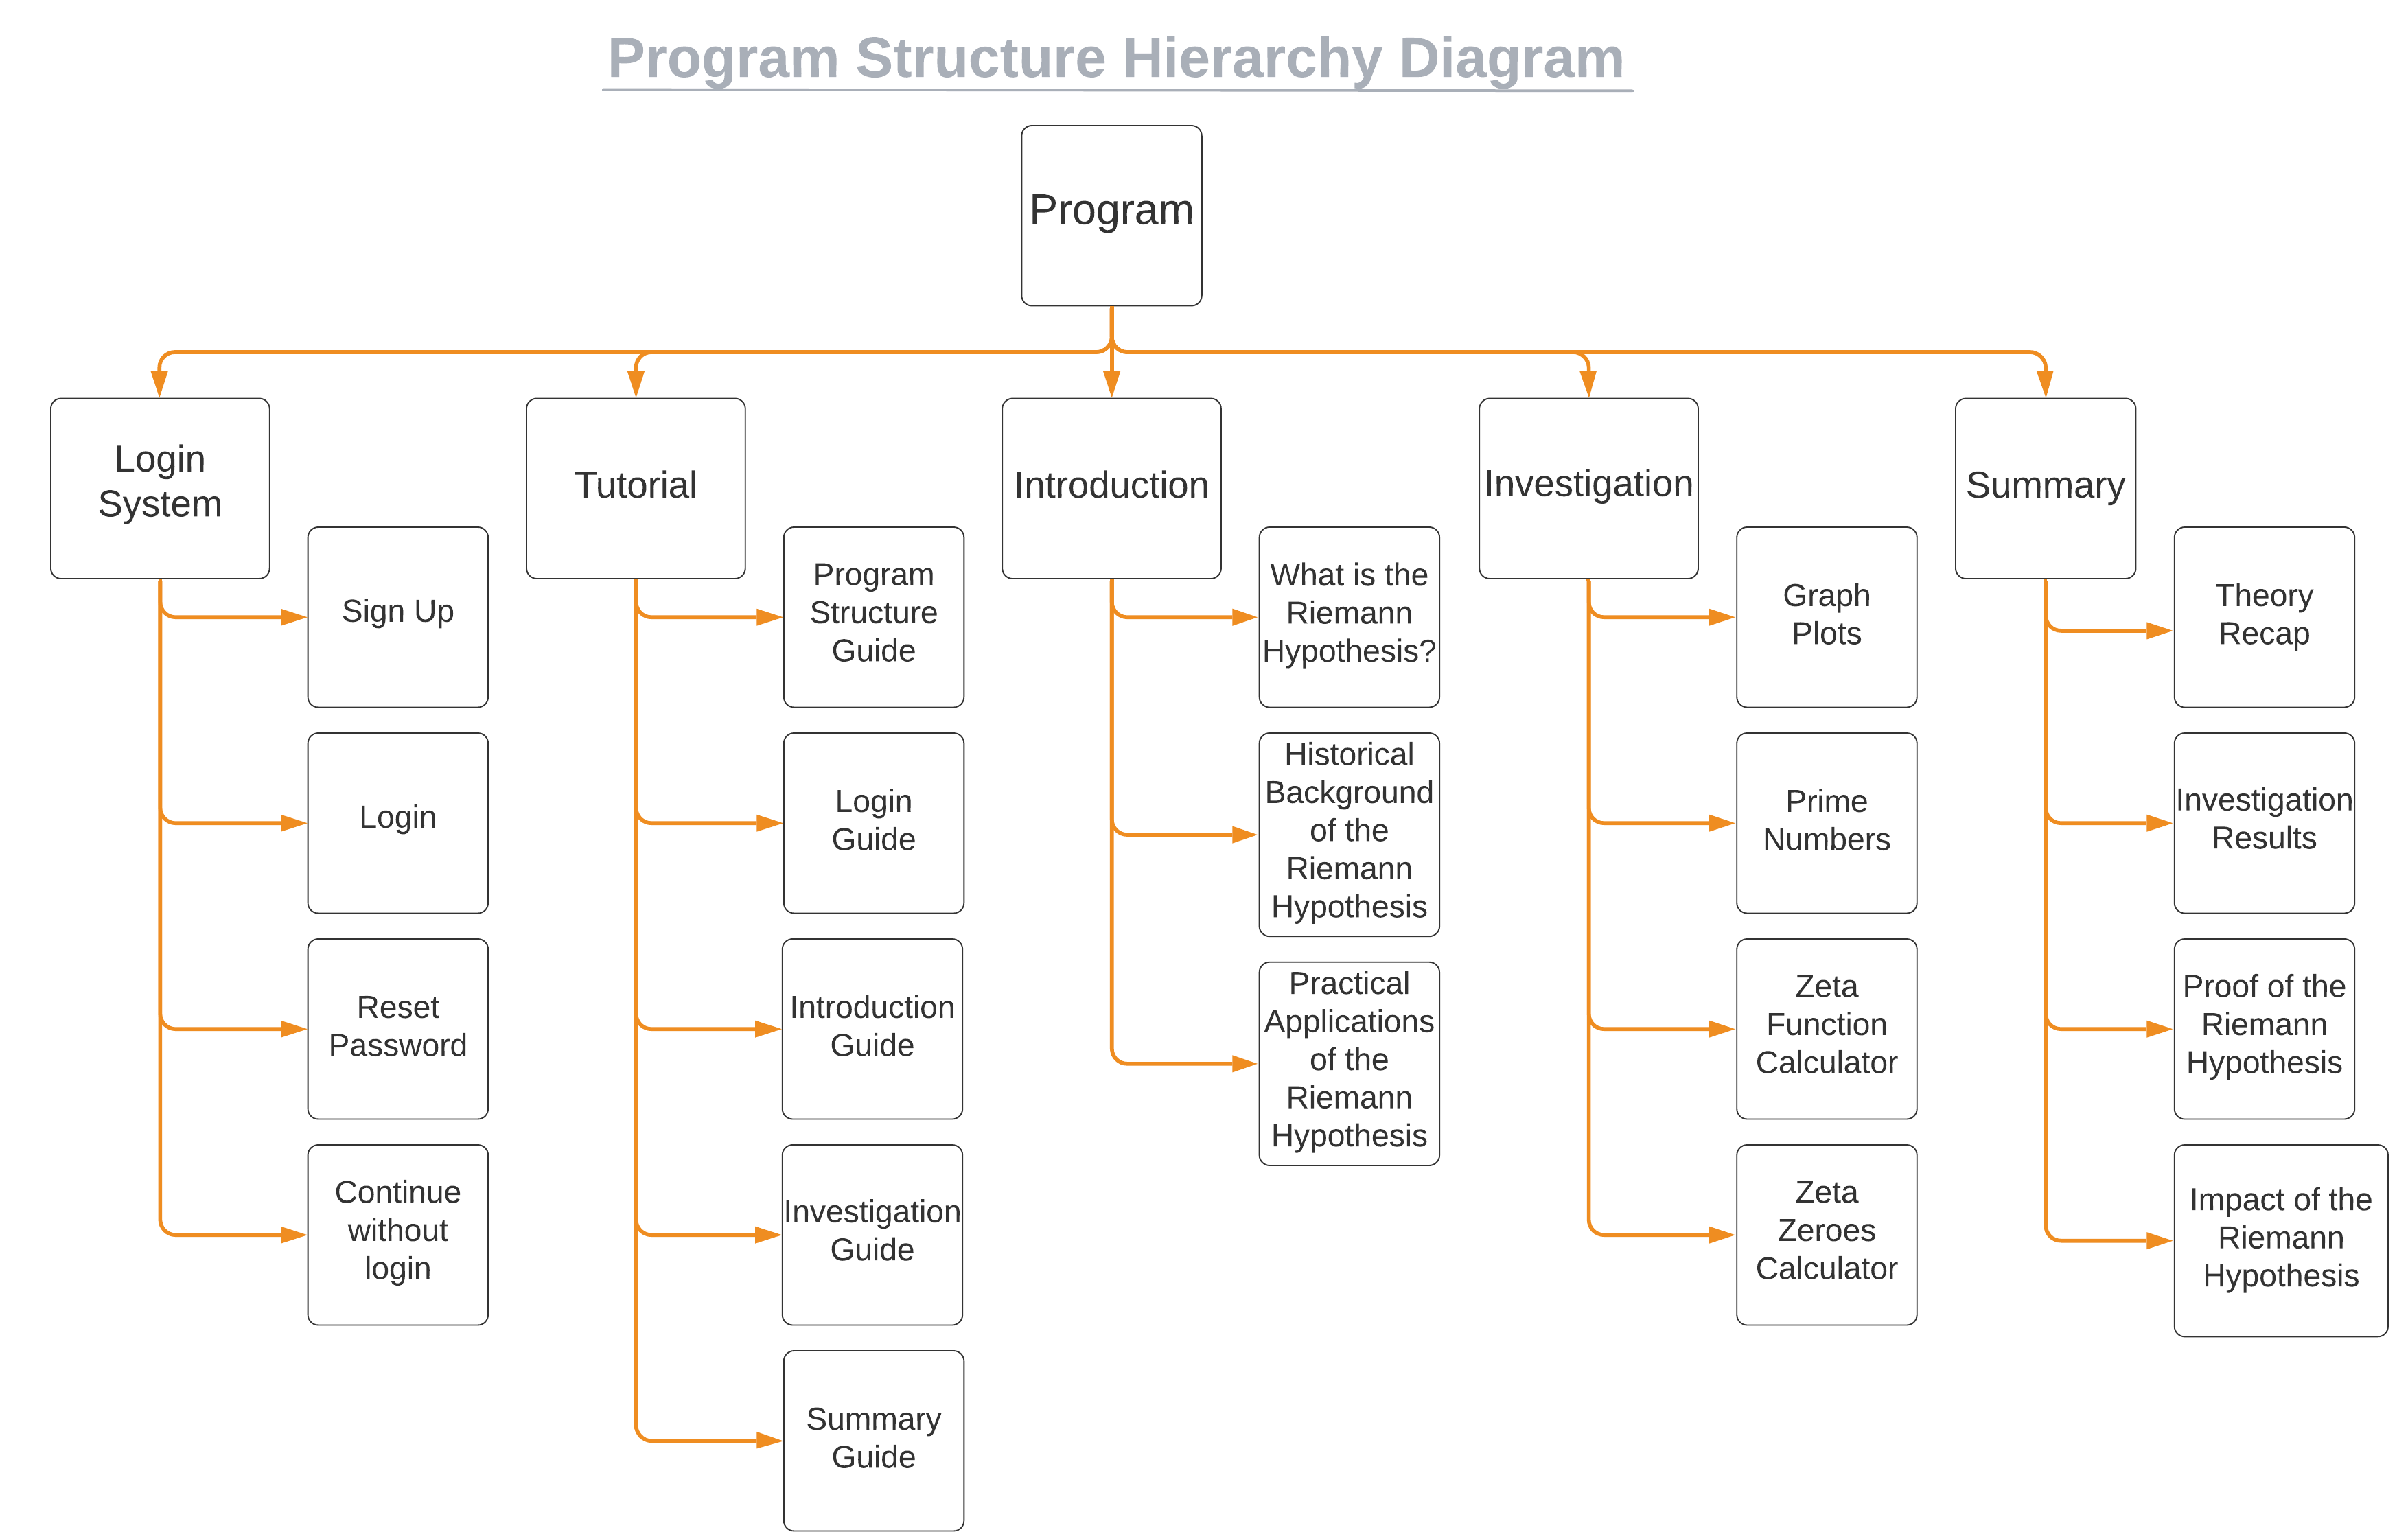
\includegraphics[scale=0.095]{program-structure-hierarchy-diagram}
    \caption{Structure Diagram for the program}
\end{figure}

As we can see from this diagram; the main program is split up into its 5 main sections: the Login System, the Tutorial, the Introduction, Investigation, and the Summary. Each of these main sections is then further broken down into its relevant subsections.

We can then break down each section into its subsections, which will in turn, be broken down into more sections.
\clearpage
\subsubsection{Login System Structure Diagram}

The login system's aim is to be able to allow a user to sign into an account, such that their progress with the program has been kept.

It will not be necessary for a user to login, however, if they do not log in, then their progress will not be saved.

\begin{figure}[h]
    \centering
    \captionsetup{justification=centering}
    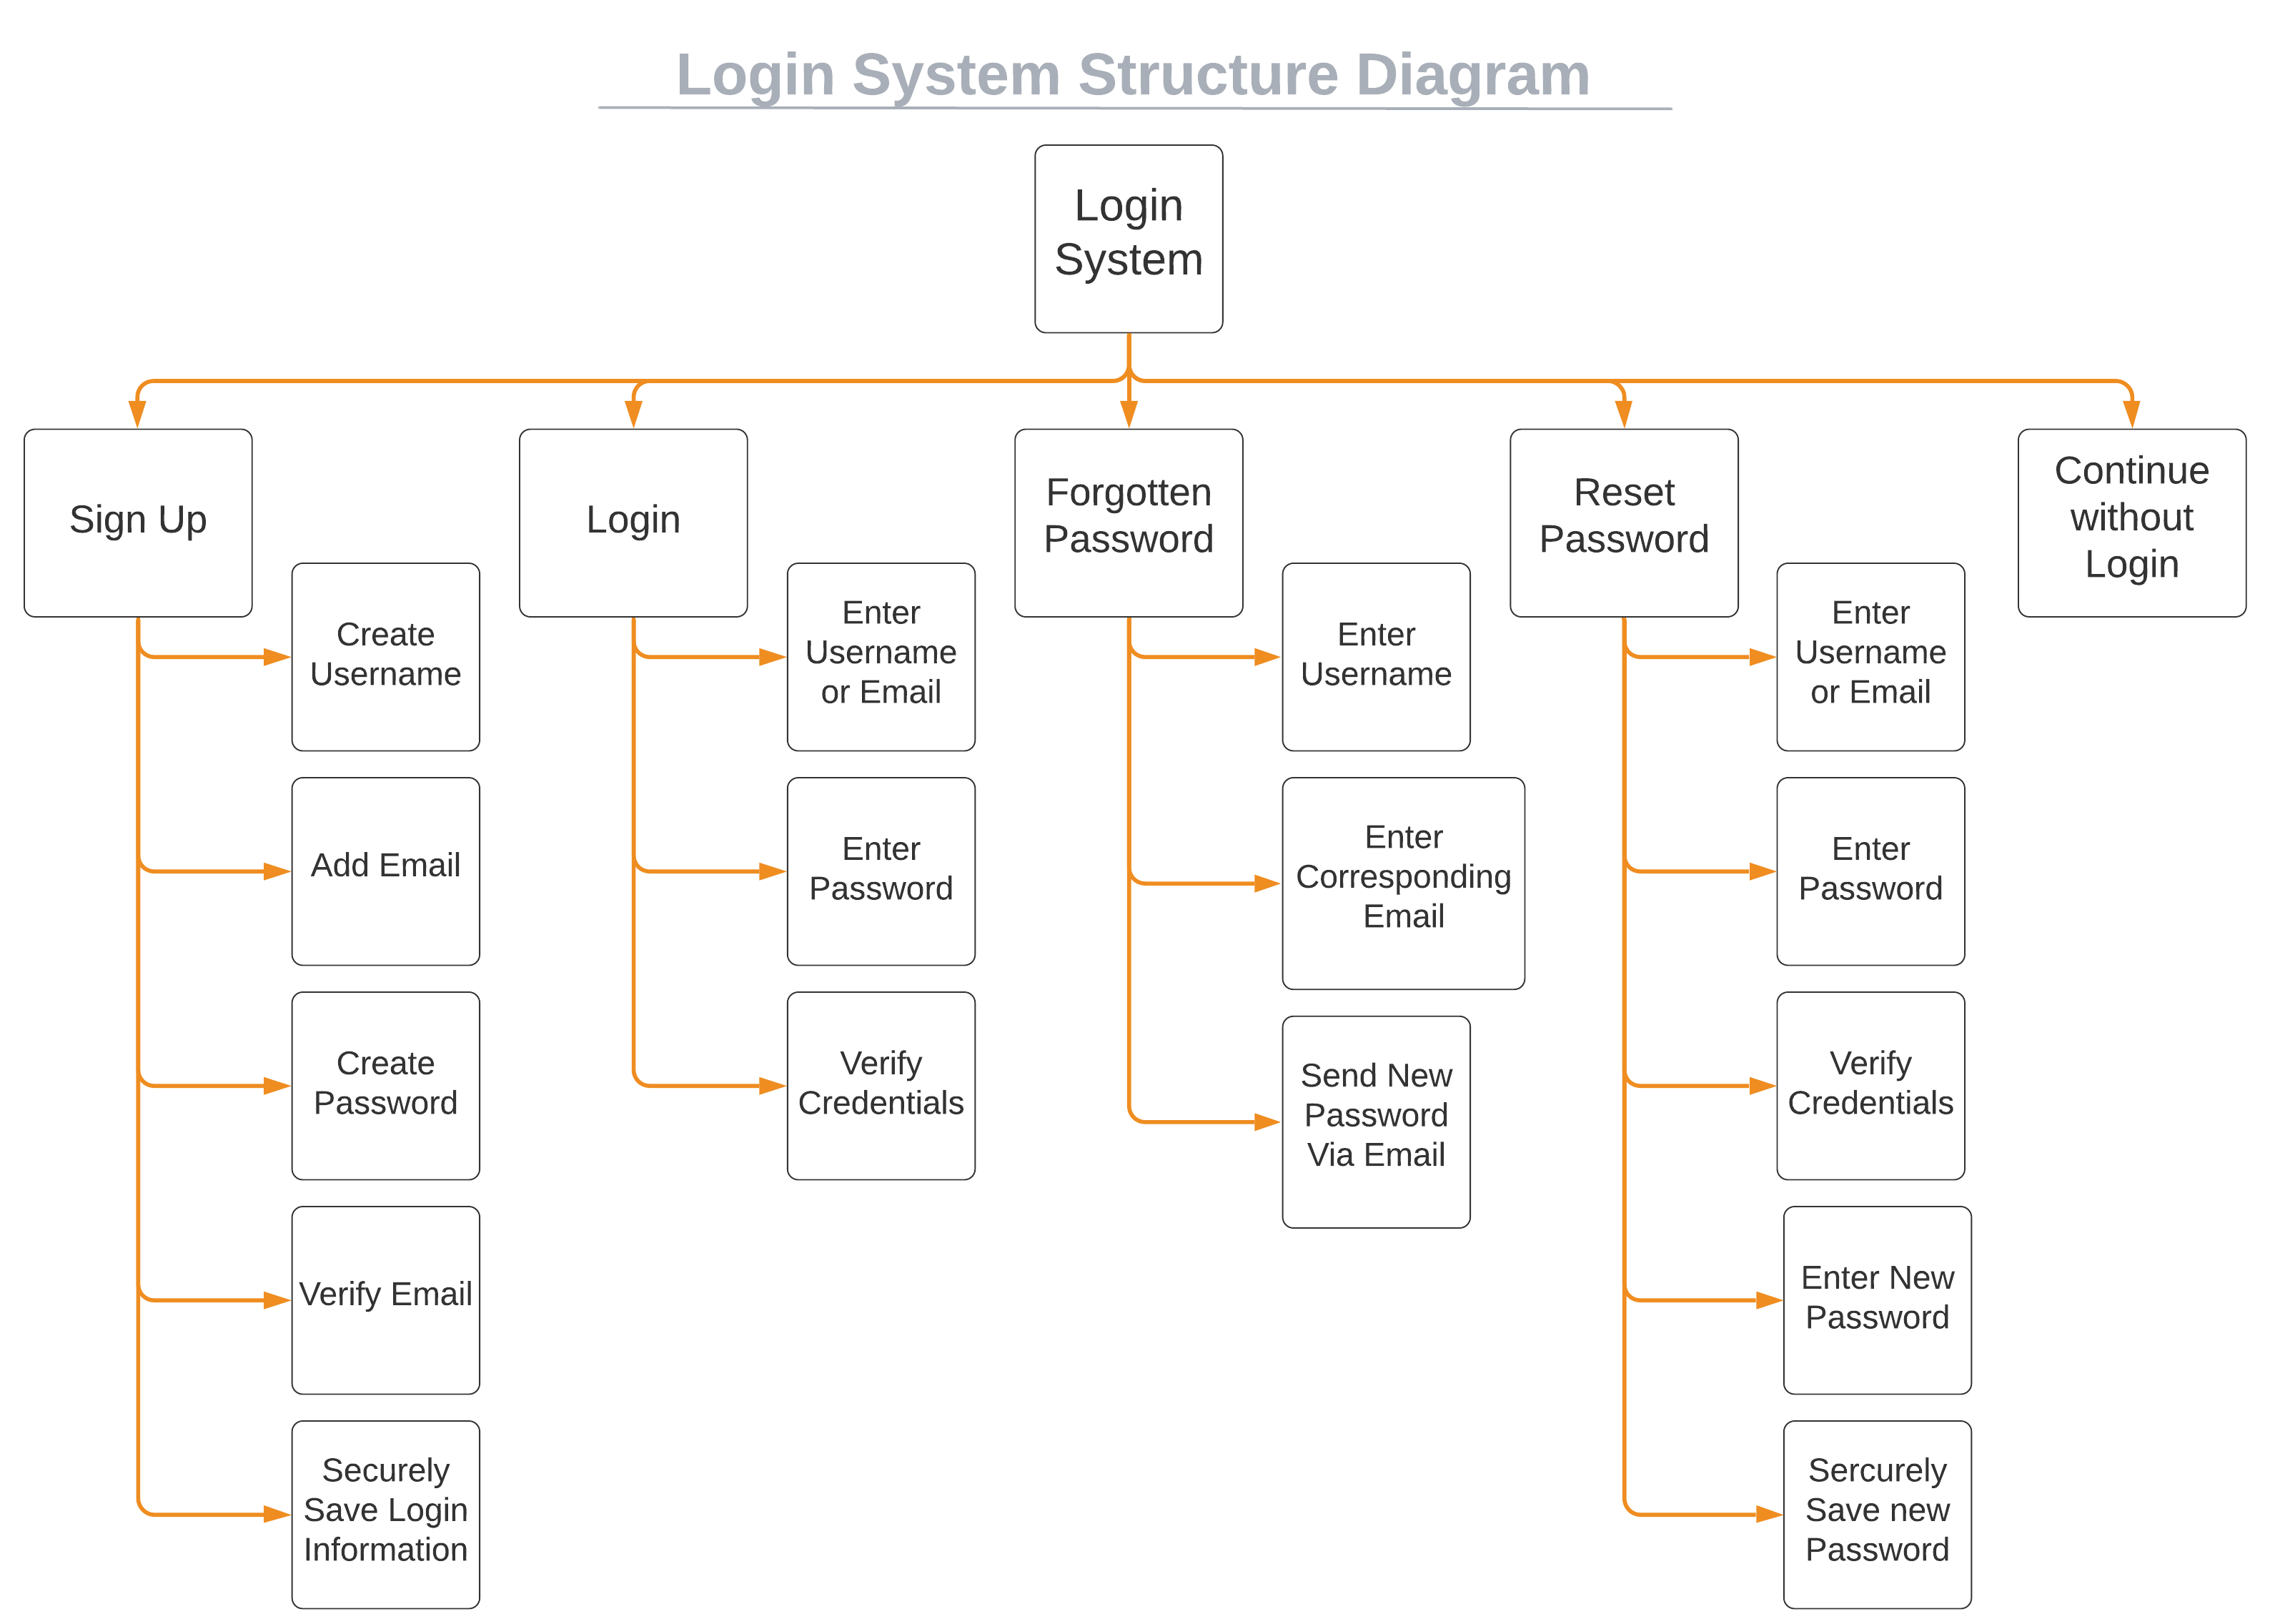
\includegraphics[scale=0.45]{login-system-structure-diagram}
    \caption{Login System Structure Diagram}
\end{figure}

There will be 5 sections to the login system that I create. The first of which allows the user to sign up and create an account. This is for first-time users of the programme, who want to be able to use it to its full functionality. The sign up process involves the user creating a unique username, adding a unique email to the account (used for when the user forgets their password), and creating a strong and complicated password. They will then be sent an email to the address that they entered, with a verification code. Once this code has been entered in the program, the user's login details will be encrypted and stored in a database. They will then advance to the next part of the program: the tutorial.

The login section will allow the user to sign in to an account that has already been created. They will be required to enter either their username or email, and their password. The program will check whether the username or email is valid (if it is in the database), and if the password associated to that account is the same as the one entered by the user. If the user gets the password wrong 3 times, then they will have to wait 1 minute before trying again. This is to stop any attacks to try and guess user's passwords. Once a user has signed in, they will be taken to the tutorial section.

If a user has forgotten their password, then they will be able to reset it in the forgotten password section. The user will be required to enter either their username and email for that account. These credentials will need to be verified, and then if they are correct, a new password will be sent to the user by email.The user will then be sent straight to the Reset Password screen so that they can change the password to one that they will remember.

The reset password section will allow the user to change their password if they don't like the one they currently have, or if they have had to reset their password. They will have to enter their username and password, to confirm their identity. They will then enter a new strong and complicated password, and this will be the new password associated to their account.

The final section is the continue without login section. Without a login, the user will still be able to use all parts of the program, however, their data will not be saved.

\subsubsection{Tutorial Structure Diagram}

The tutorial is one of the key sections of the program. The tutorial will give the user a guide on how to use the program.

\begin{figure}[h]
    \centering
    \captionsetup{justification=centering}
    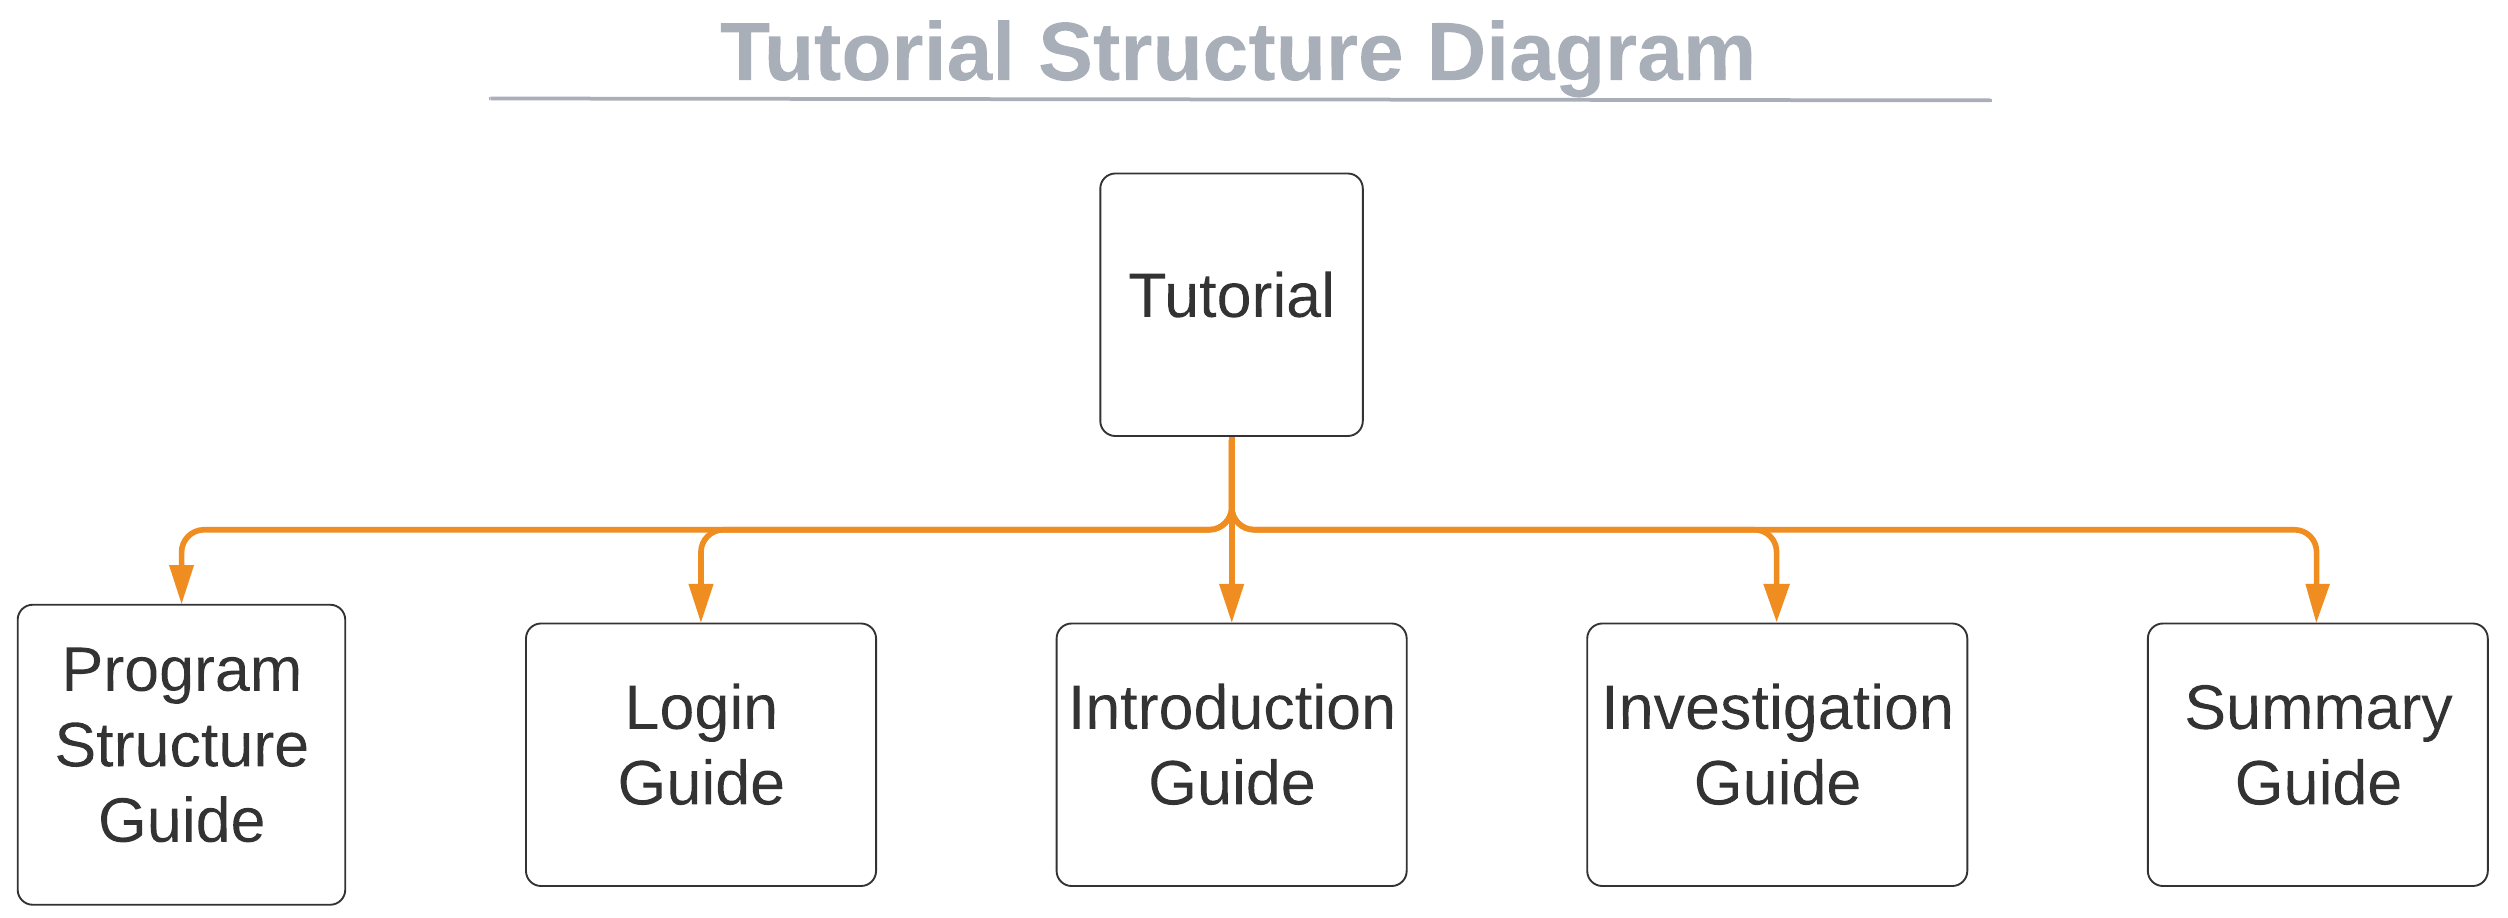
\includegraphics[scale=0.55]{tutorial-structure-diagram}
    \caption{Tutorial Structure Diagram}
\end{figure}

The tutorial itself will be split up into 4 main parts; that is a guide on the structure of the program, and how to use each of the individual sections of the program.

Overall, the tutorial will be relatively simple, and will just give the user an understanding of how to use the program

The Program Structure Guide will inform the user of the layout of the project, and how each section is related to another. It will tell the user how to navigate pages, and how to use key features of the program that will require user input.

Next in the tutorial, will be the Login Guide. This will essentially just be a quick note to the user, about how to sign up and create a strong and complicated password, what to do if you forget your password, or want to change it; as well as explain why the user may or may not want to create an account, and how the program differs whether the user is signed in or not.

As for the Introduction Guide, it will show an example of what the introduction section will look like, and have labels to show how to navigate pages as well as what everything means.

Probably the most complex part of the tutorial section will be the Investigation section. This will inform the user of how to use, understand, and interpret the different graphs and plots. This section should give the user a simple understanding of how they can use the program to investigate the Riemann Hypothesis

The final section in the tutorial will be a Summary Guide, that is how to use the summary section of the program. This will be very similar to the Introduction Guide, but will have an emphasis on the user trying to draw conclusions from the data they have collected, instead of the just being able to understand what is going on.

The tutorial section will not have a lot of functionality, but its purpose is just to briefly describe to the user, how the program is intended to be used.

\clearpage

\subsubsection{Introduction Structure Diagram}
In the Introduction section of the program, the user will be able to develop their understanding of what the Riemann Hypothesis is and why its so important.

I will portray this information by splitting the Introduction into three smaller sections. You can see how this section will be split up in the Structure Diagram below:

\begin{figure}[h]
    \centering
    \captionsetup{justification=centering}
    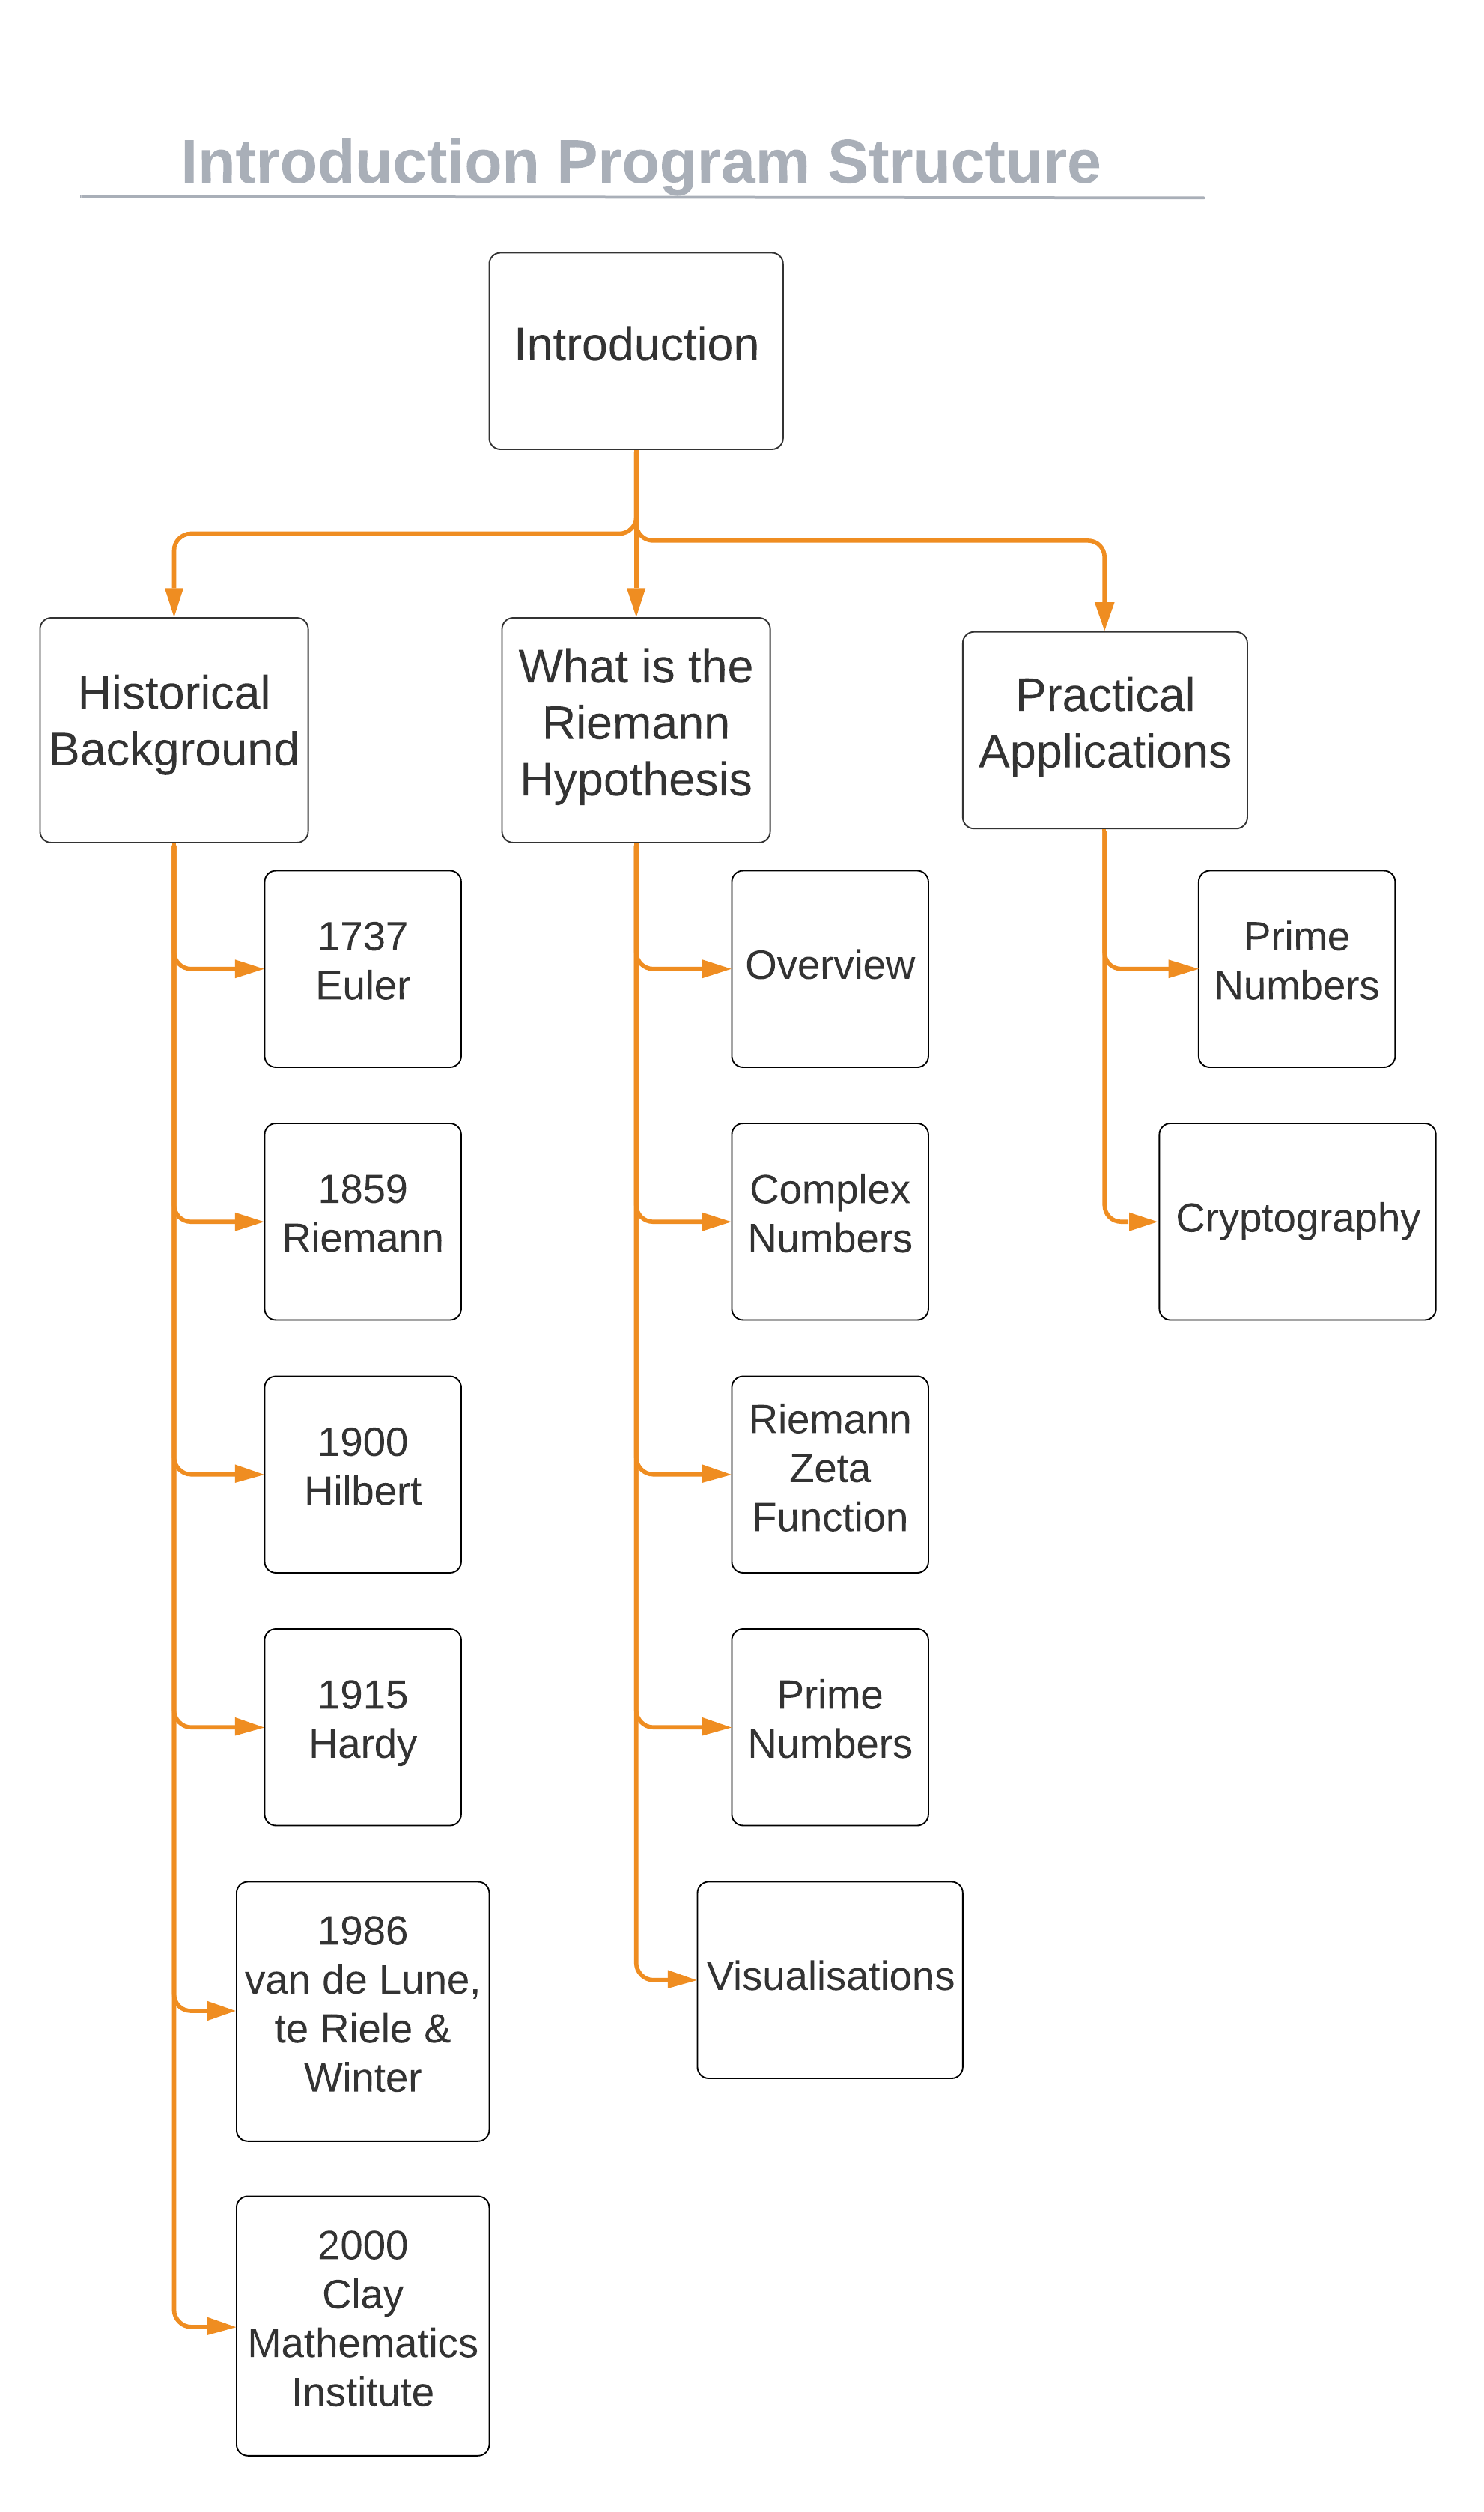
\includegraphics[scale=0.385]{introduction-structure-diagram}
    \caption{Introduction Structure Diagram}
\end{figure}

First of all is the historical background section. This shows how the Riemann Hypothesis has developed over time and showcases the context of the problem

Next is the section describing the Riemann Hypothesis. This section will include a lot of maths, but will also be written such that people will a limited mathematical understanding will still be able to understand what is being said.

The final part of the introduction is the Practical Applications section. This will inform the user why the Riemann Hypothesis affects us today and how it can actually be used.

\clearpage
\subsubsection{Investigation Structure Diagram}
The Investigation is the main part of the program and will allow the user to conduct their own research into the Riemann Hypothesis.

It will have 4 main section; The graphs, Prime Numbers, a zeta function calculator, and a zeta zeros calculator.

\begin{figure}[h]
    \centering
    \captionsetup{justification=centering}
    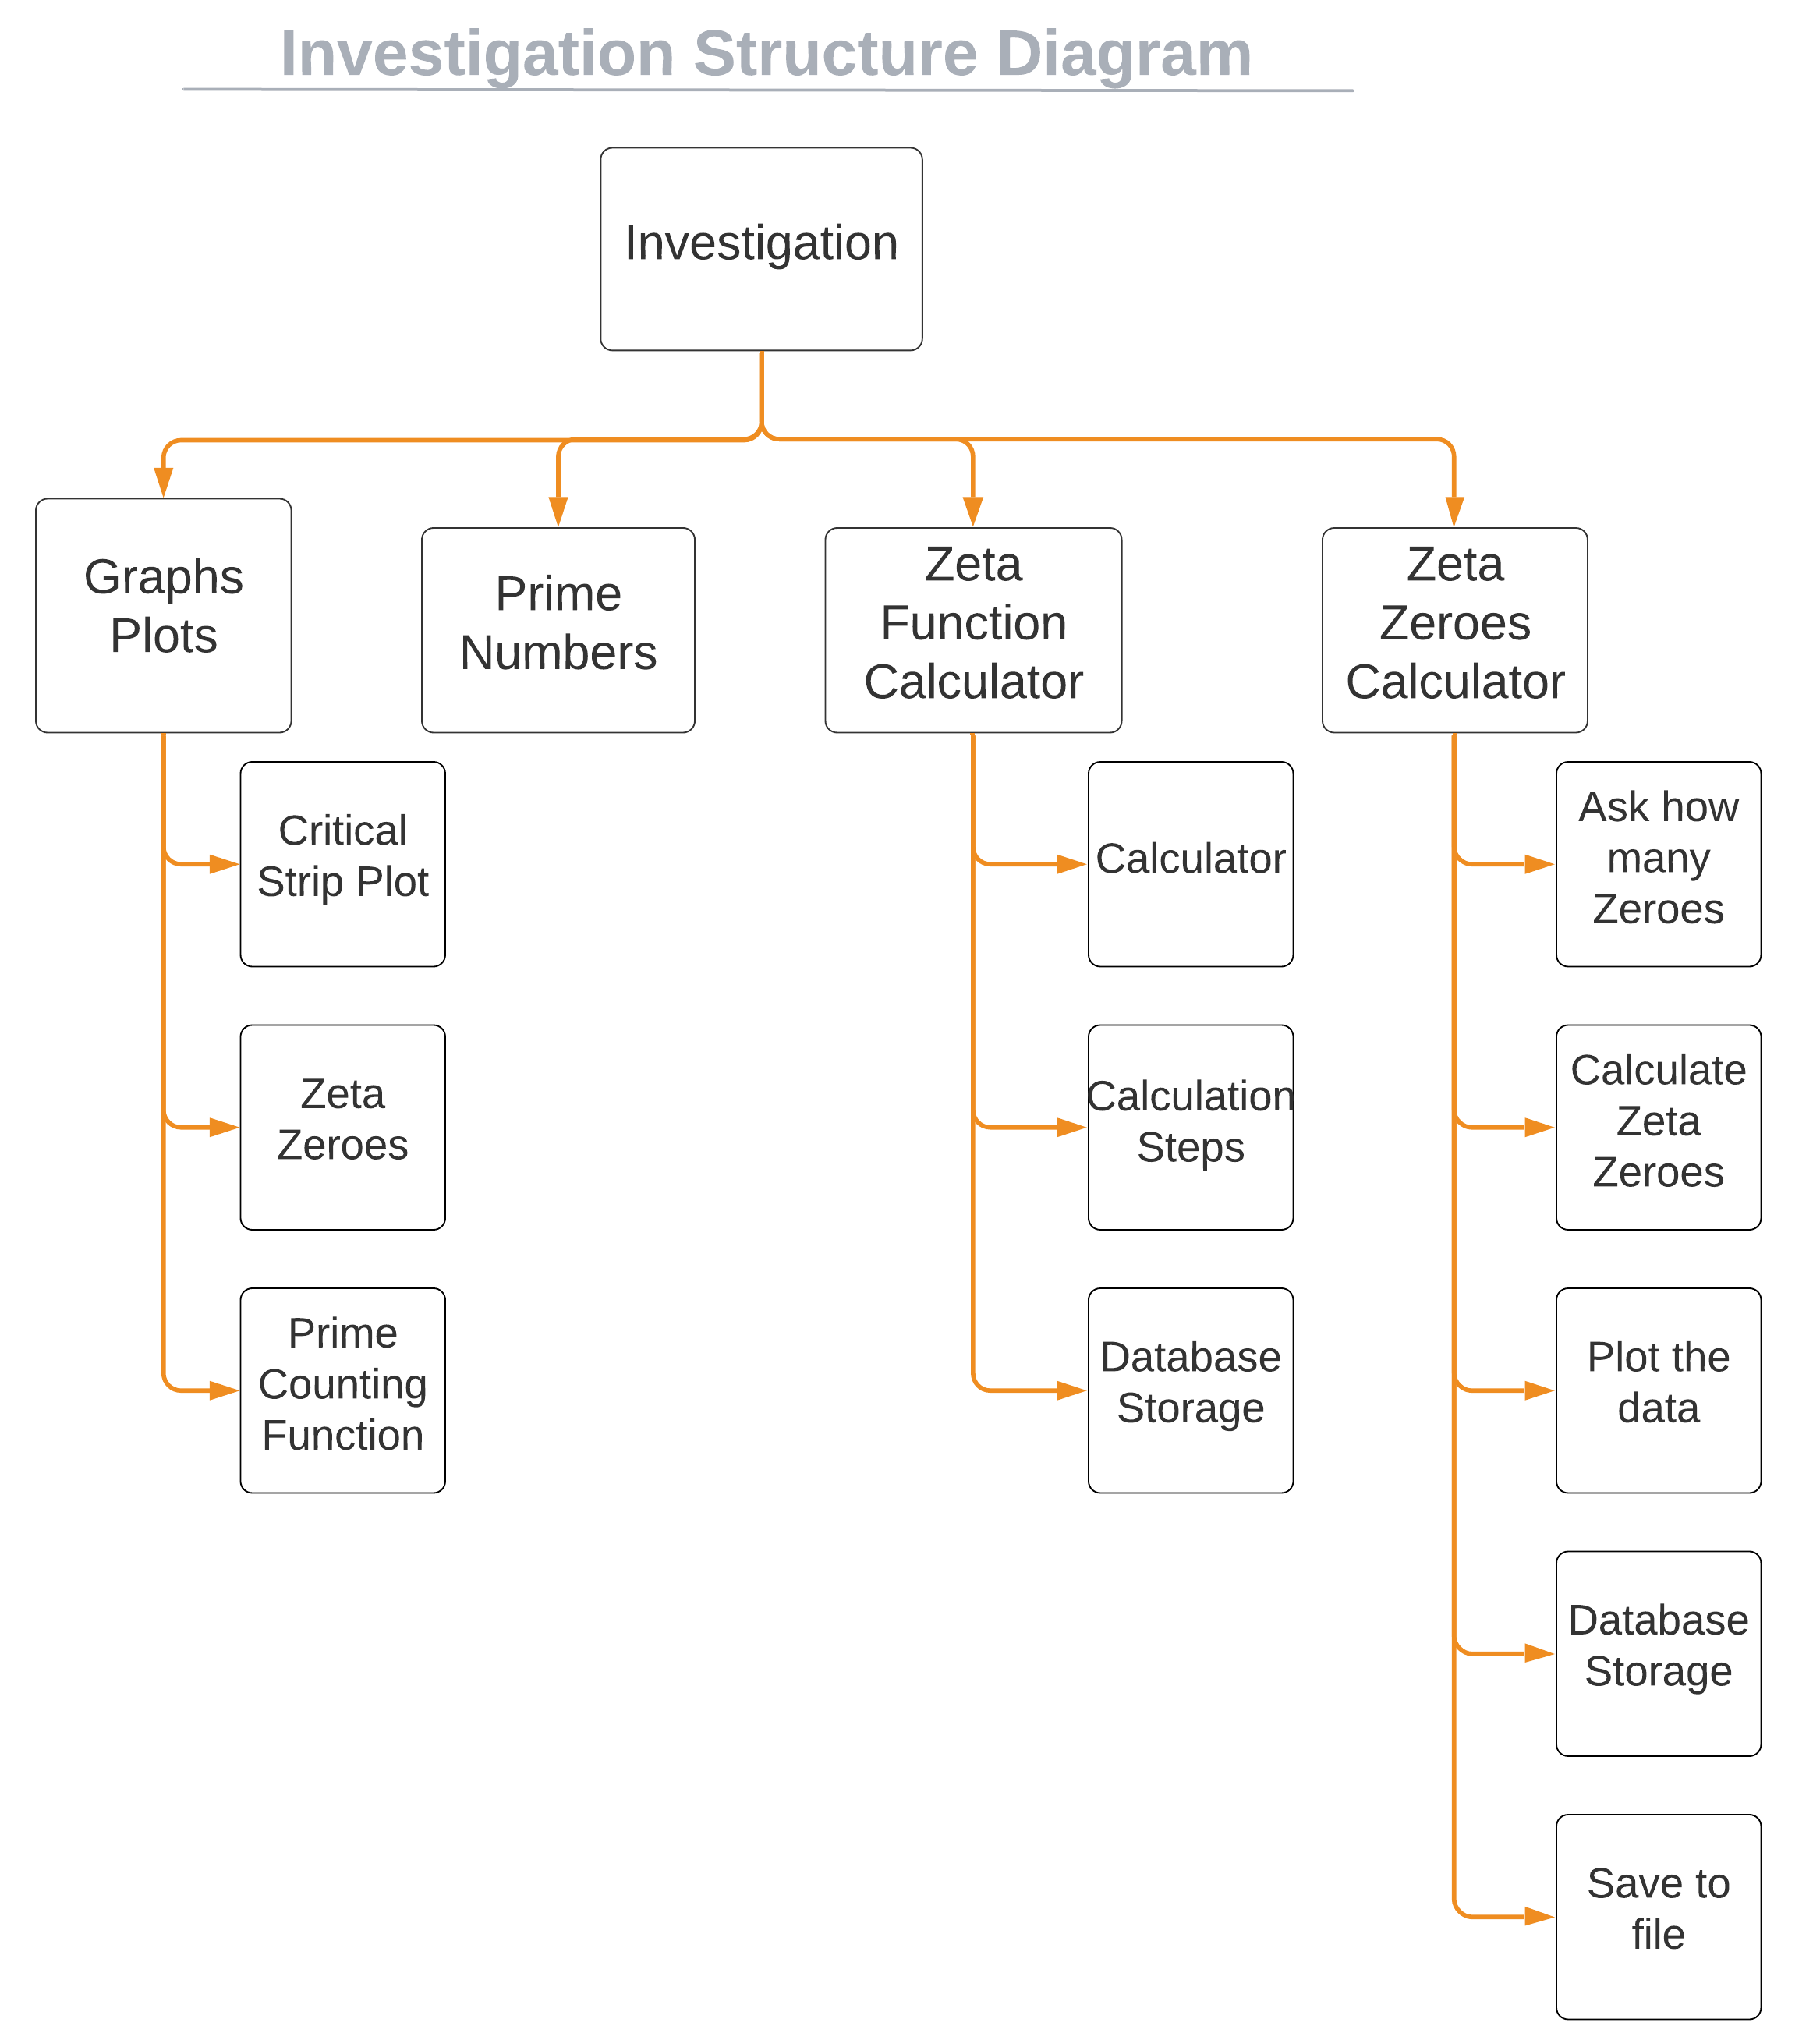
\includegraphics[scale=0.5]{investigation-structure-diagram}
    \caption{Investigation Structure Diagram}
\end{figure}

The first section will be the Graph Plot section. The aim of this section is to display to the user various graph plots that are related to the zeta function. This user will be able to change given inputs into the graph plots and be able to see the output visually.

The prime number section will show the user the correlation between the Riemann Zeta Function and the prime numbers. This section will showcase various graphs and mathematical functions for the user to explore.

Next is the zeta function calculator. This will be a relatively simple part of the investigation section. It will allow the user to input a number (or range of numbers)into the calculator. It then calculates these values and will allow the user to store the data, either in a file or database.

Finally is the zeta zeroes calculator. This will calculate all of the zeta zeroes between two points given by the user, and with accuracy determined by the user. Similarly to the zeta function calculator, the user will also be able to store this data to a database or file, or even display the data in a graph plot.


\subsubsection{Summary Structure Diagram}

The final main section in the program will be the summary. It will be a recap of what the user should have learnt from using the program, and what to take away from it. It will be split up into a theory recap section, a results section, a conclusion and evaluation section and a section on the impact of the Riemann Hypothesis.


\begin{figure}[h]
    \centering
    \captionsetup{justification=centering}
    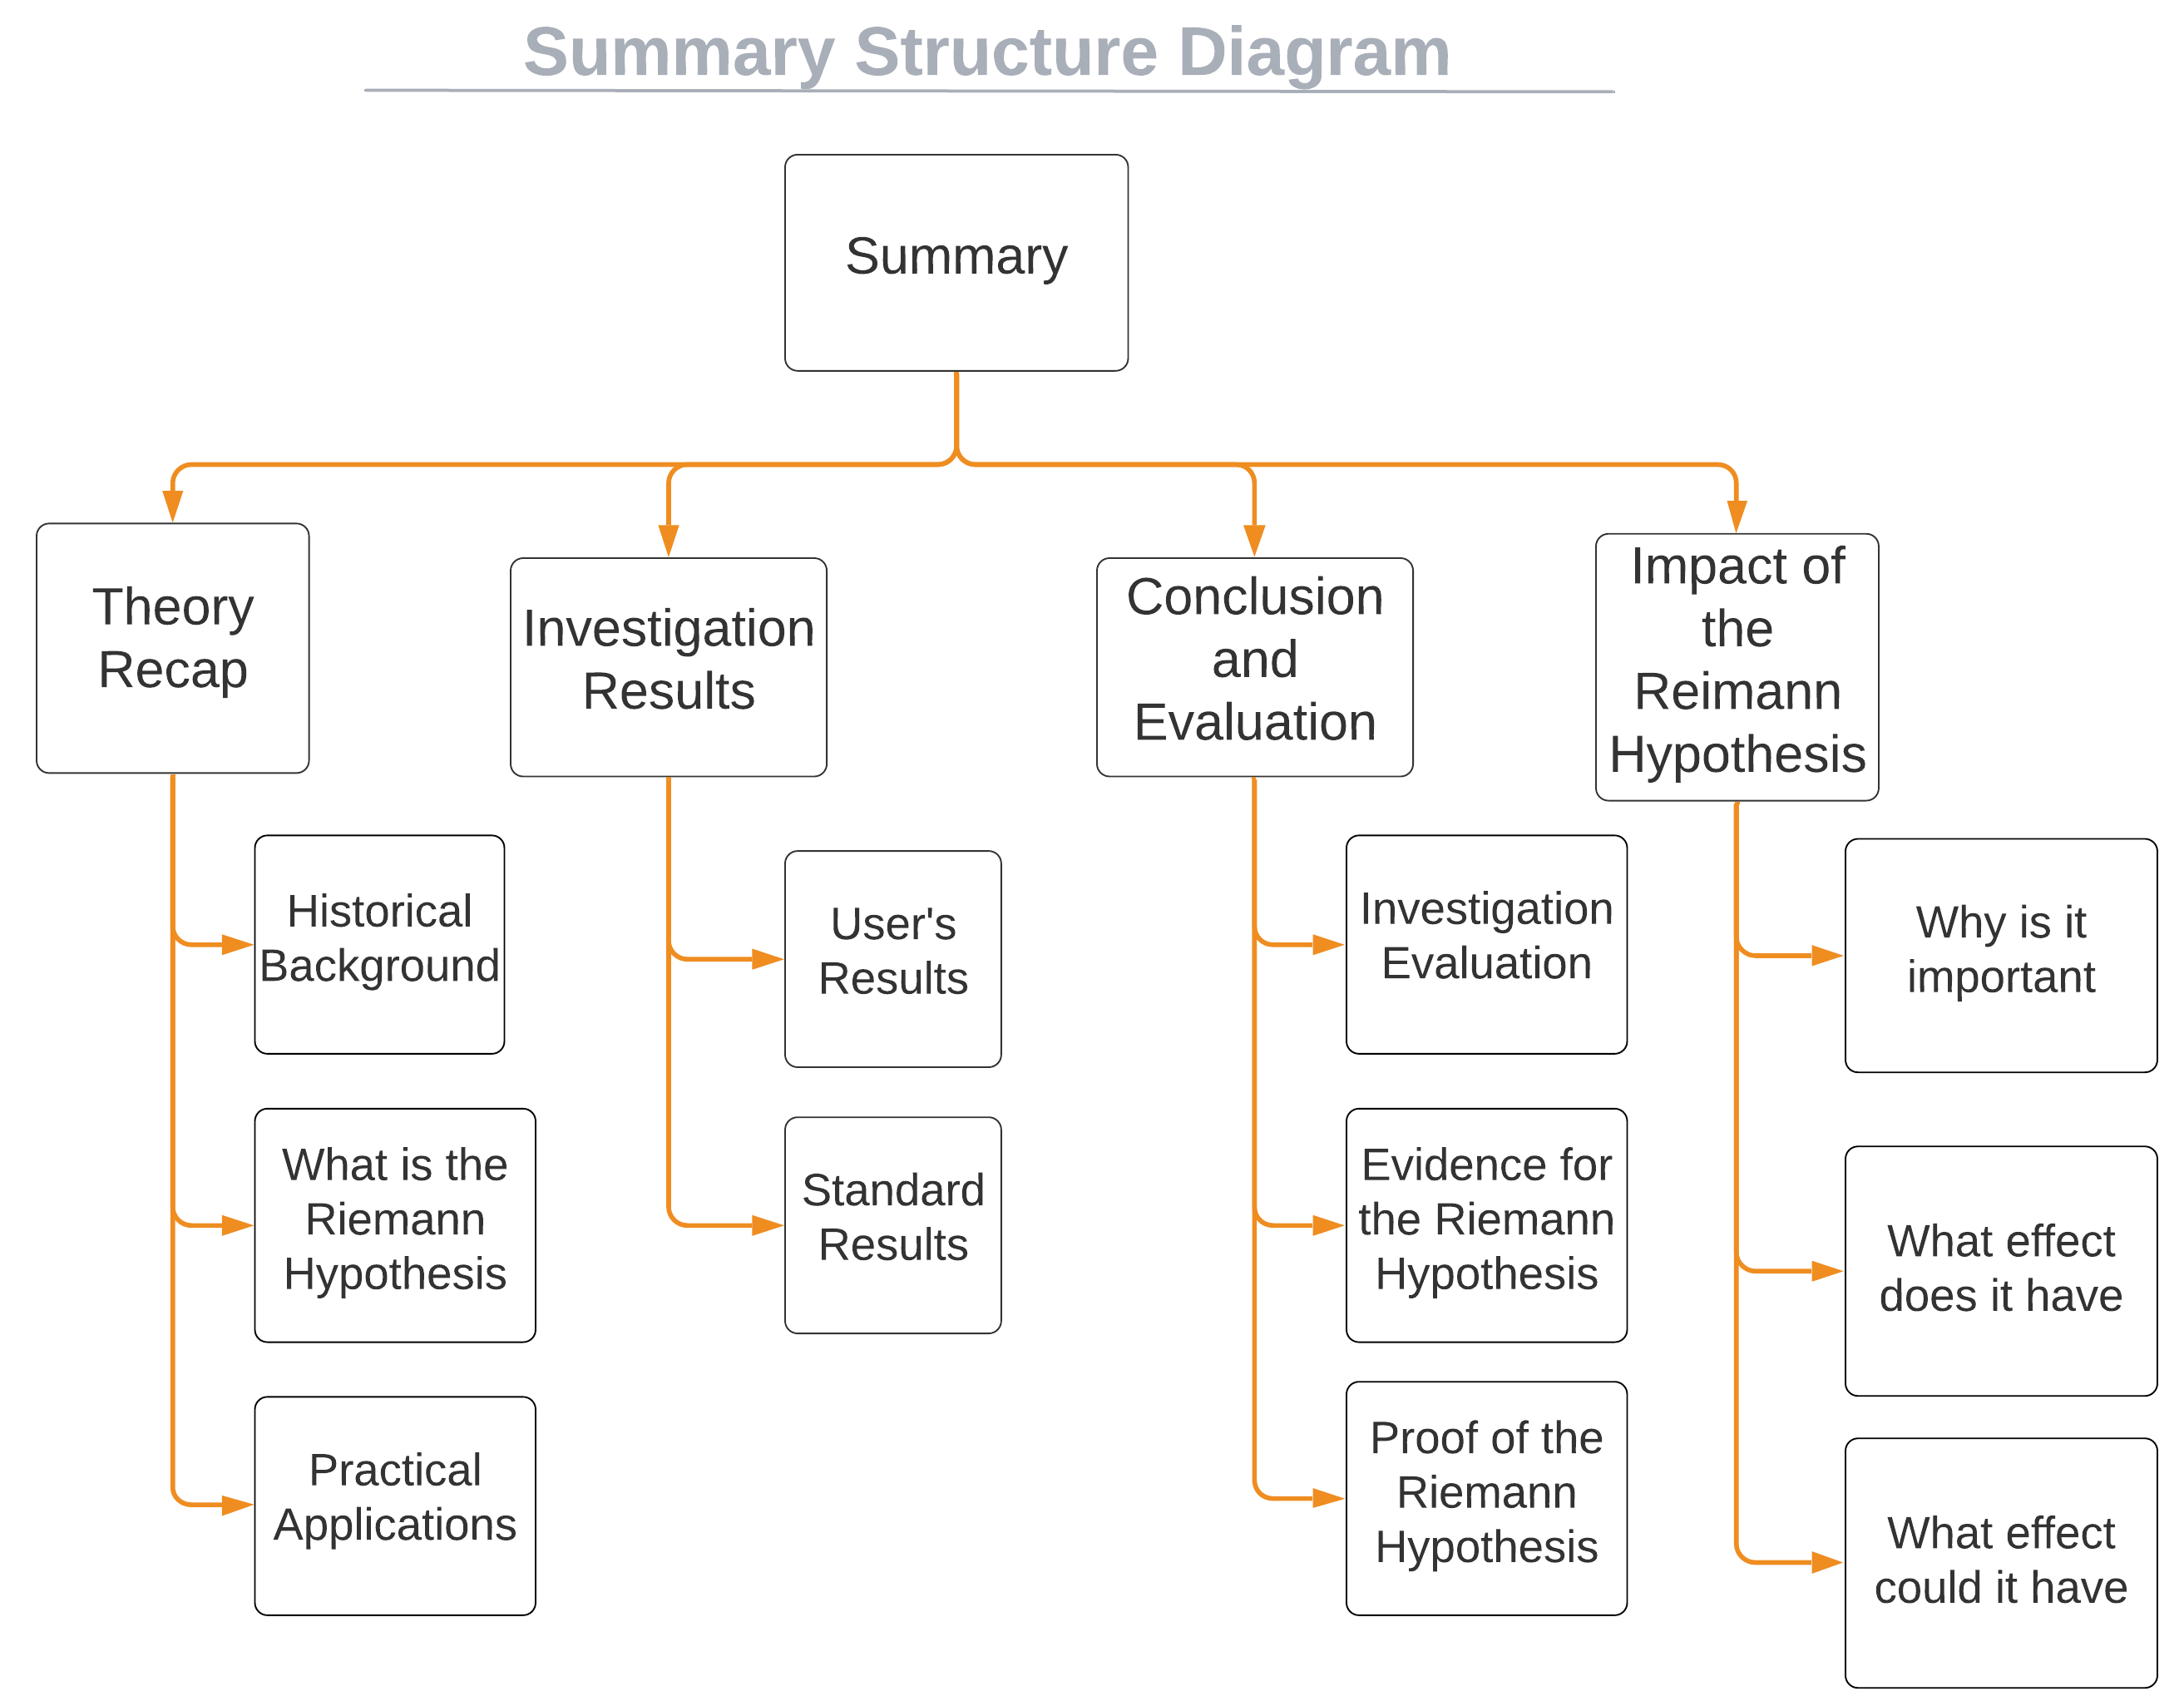
\includegraphics[scale=0.5]{summary-structure-diagram}
    \caption{Summary Structure Diagram}
\end{figure}

The first part of the summary; the theory recap will essentially be a very cut down version of the introduction section. It will provide an overview of the problem such that the user can refresh their mind as to what the Riemann Hypothesis actually is.

As for the investigation results, this page aims to provide the results of the user's investigation. It will provide raw data as well as some visual aids such as graphs. It will also compare the data collected by the user with the expected data.

Next is the conclusion and evaluation section. This section will detail to the user how accurate their results were to the true values, as well as any evidence and proof of the Riemann Hypothesis.

Finally, is the Impact of the Riemann Hypothesis. The aim of this section is to explain to the user why the Riemann Hypothesis is so important by explaining how it affects us.


Overall, I feel as if I have sufficiently broken down my project into a number of more manageable parts that will comes together neatly to form the whole system.
% \subsection{Hierarchy Diagrams}

% \subsection{System Flowcharts}

% \subsection{Data Flow Diagrams}

\clearpage
\subsection{Object-Oriented Design}

\begin{figure}[h]
    \centering
    \captionsetup{justification=centering}
    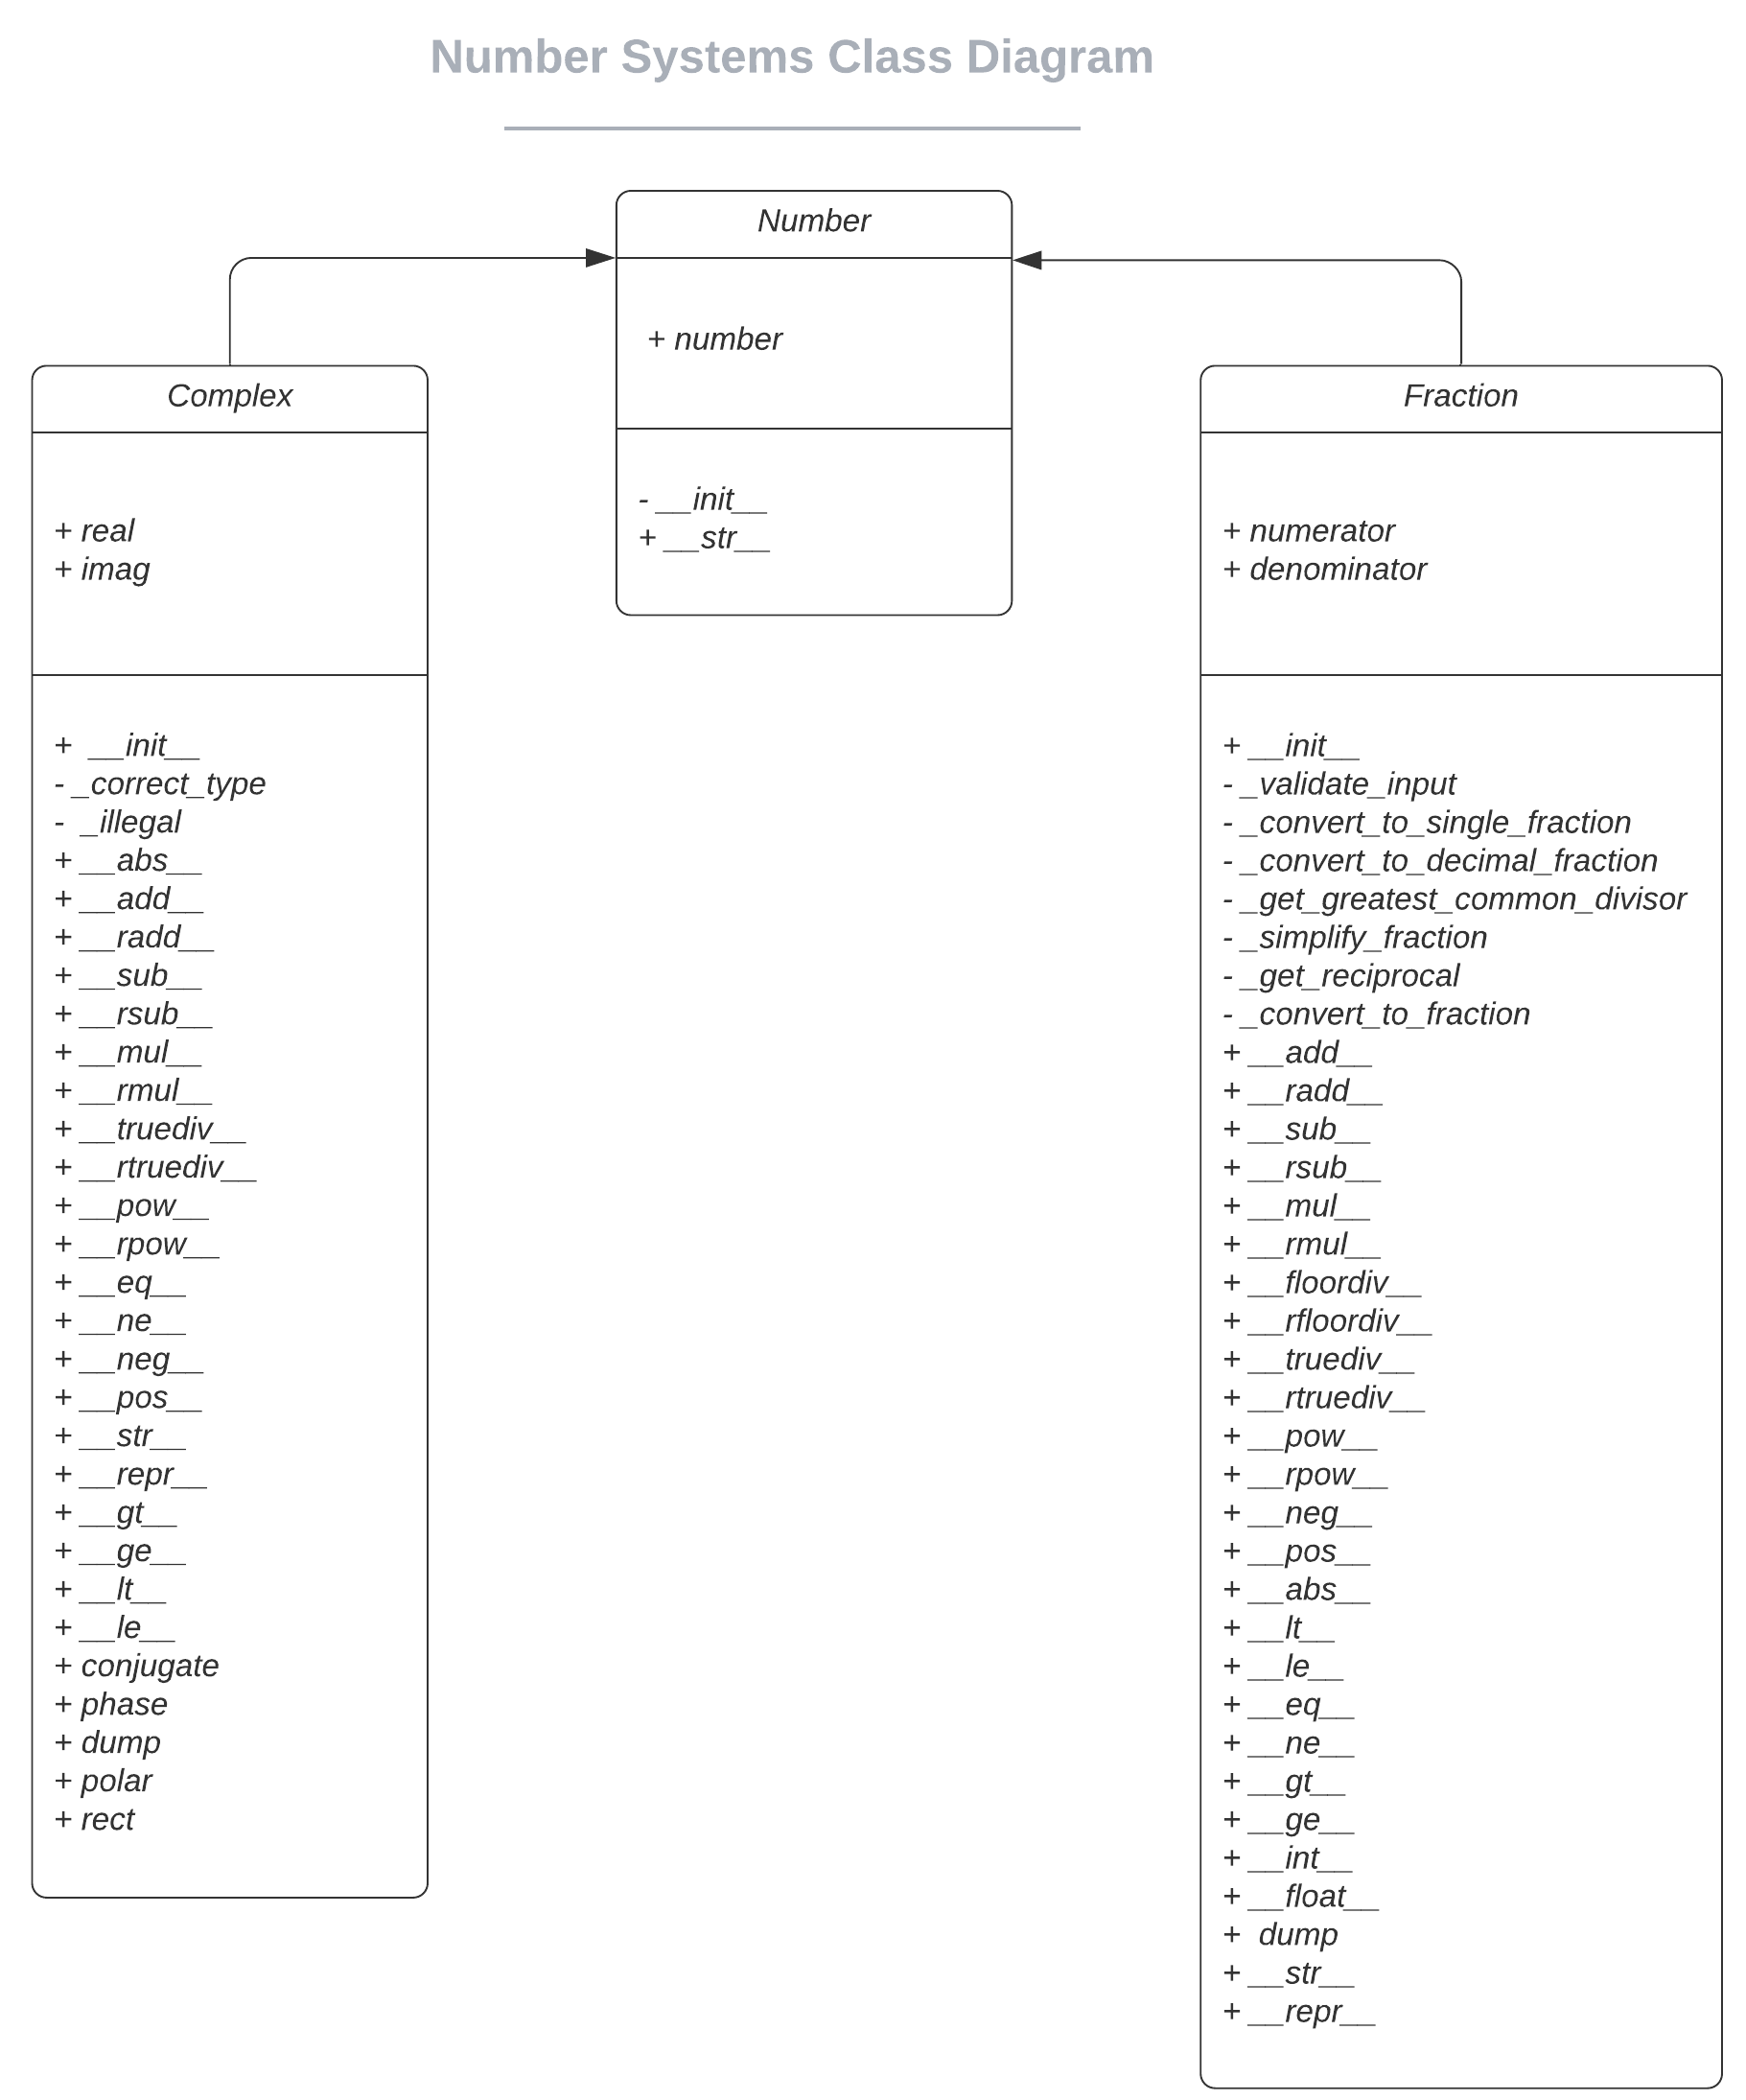
\includegraphics[width=6in]{number-systems-class-diagram}
    \caption{Number Systems Class Diagram}
\end{figure}
As part of this project I will need to be able to represent many types of numbers namely, fractions and complex numbers. The best way to do this is to use Classes and Object-Oriented Programming. I can create a data structure in python, such that they will be able to store all of the necessary data, and perform all the operations that I need.

All of the data types will inherit attributes and methods from a main \textit{‘Number’} Class. This number class will have basic attributes and methods, allowing a number to be defined and printed.
\clearpage
The complex number class is a lot more substantial than the number class.  It will allow for inputs in Rect form, or Modulus Argument Form. The methods in this class will allow for the user to add, subtract, multiply, divide, and use exponentials with complex numbers. There will also be a set of private functions in the class in order to change between cartesian and polar form.

As for the fraction class, it will take inputs of a numerator and denominator, and will allow the user to use public functions in order to perform operations and calculations involving fractions.

These classes will be able to let me sufficiently perform precise calculations with numbers. The fraction class removes any mathematical floating point errors from calculations, and the complex class will allow me to utilise imaginary and complex numbers in Python.

Some points to note; I have tailored this class diagram and the following pseudocode for a Python programme. Conventionally, when calling a function prefix notation is used. For example, if we have a simple function as follows:

\begin{algorithm}
    \caption{Prefix add function}
    \begin{algorithmic}
        \Function{add}{$a$, $b$}\\
             \hspace{\algorithmicindent}\Return $a + b$
        \EndFunction
    \end{algorithmic}
\end{algorithm}

Then we can see that it takes two inputs, a and b, and will return their sum.

To call this function, we will use prefix, notation with the function name at the beginning, followed by the two parameters.
Such as:

\begin{algorithm}
    \caption{Calling the prefix add function}
    \begin{algorithmic}
       \State \Call{add}{$a$, $b$}
    \end{algorithmic}
\end{algorithm}

However, in Python, we are able to create mathematical functions that allow for infix notation. This is a more natural way of calling maths functions. To allow for infix notation, we add two underscores to the beginning and end of the function name when we define it. So for some example python code:


\begin{lstlisting}
# Python infix add function
def __add__(a, b):
    return a + b
\end{lstlisting}

We can run it by calling

\begin{lstlisting}
# Python call infix add function
    a = 1
    b = 2
    c = a + b
\end{lstlisting}

Which is infix notation. Now in this example, it may seem almost obsolete to create a function that already mimics the behaviour of what we are trying to achieve, however using this notation we are able to overwrite the existing infix notation in python, and even create new notation of any data types that we choose to create.

A simple example of this is with the fraction class. There is no inbuilt class for handling fractions in python, so we can create one and allow it to use infix notation.

If we have a fraction class that takes a numerator and denominator as an input, and have this function defined in the class, it would look as follows:


\begin{lstlisting}
# Python __add__ as part of the Fraction Class
def __add__(self, other):
        """ self + other """
        other = self._convert_to_fraction(other, 'addition')
        resulting_numerator = self.numerator * other.denominator +
                              self.denominator * other.numerator
        resulting_denominator = self.denominator * other.denominator
        return (Fraction(resulting_numerator, resulting_denominator))
\end{lstlisting}

This function finds a common denominator for the fractions and then adds the numerators together.

To call this function to add $\frac{3}{4}$ and $\frac{1}{2}$ , we would use infix notation as follows:


\begin{lstlisting}
# Python calling __add__ for two instances of the class Fraction
Fraction(3, 4) + Fraction(1, 2)
\end{lstlisting}

Which would return the correct value of $\frac{5}{4}$.

As we can see from this example, we have created a python function that can be called using infix notation, rather than the standard postfix notation.

One other point to note is that python does not handle infix notation for user defined data types very well. If we want to compute the user defined \textit{Fraction} + the Python Integer $3$, this is okay. But due to the way python has been created, we would be unable to do Integer $3$ + \textit{Fraction}. For this we need to define another function called \textit{\_\_radd\_\_}, short for right add. This allows us to still compute the infix addition, even when the user defined variable is on the right hand side of the addition sign. The \textit{\_\_radd\_\_} function would use the already created \textit{\_\_add\_\_} function, but would have its arguments swapped and the code would look as follows:

\begin{lstlisting}
# Python infix radd function
def __radd__(self, other):
        """ other + self """
        return self.__add__(other)
\end{lstlisting}

This would swap the arguments around so that the \textit{\_\_add\_\_} function is then called with the parameters in the correct position.

\clearpage
\subsection{Database Design}

Throughout this next section, I will be explaining the structure of the database I will be using, creating data tables for each of the tables in the database, create designs for the key SQL queries that will be used, and I will create entity-relationship diagrams for the database.

\subsubsection{Table Designs}
In this subsection, I will be using data tables to represent the tables that will be present in my database.

Within my database, there will be 8 tables, which are:

\begin{enumerate}
    \item Users Table
    \item Questions Table
    \item Answers Table
    \item User Answer Table
    \item Notes Table
    \item Notes Responses Table
    \item Zeta Table
    \item User Zeta Table
\end{enumerate}

In each data table, I will show the table name and the name of each of the fields in the table. For each of the fields, I will list whether it is a key of the table, it's datatype, any necessary validation using regular expressions, and some notes on the field.

With the regular expression used for validation, an item in the table will only be considered valid if the entire item itself is a match to the regex. For strings, I am limiting their size to 140 characters, such that the user will be unable to enter strings that are too long and potentially use up too much storage in the database.

\clearpage
\textbf{Users Table}

The purpose of the Users Table will be to store the login credentials for each user registered to the program. The table will store the username, email, and hashed password of each of the users. This is the table that will be referenced when a user creates an account, or goes to login to an existing account.

\begin{table}[ht]
    \centering
    \begin{tabular}{ | p{0.15\linewidth} | p{0.1\linewidth} | p{0.16\linewidth} | p{0.14\linewidth} | p{0.25\linewidth} | }
    \hline
    \multicolumn{5}{|c|}{\textbf{Table: Users}}\\
    \hline
    \hline
    \textbf{Field} & \textbf{Key} & \textbf{Data Type} & \textbf{Validation} & \textbf{Notes} \\
    \hline
    User\_ID & Primary & Integer & & \\
    \hline
    Username & & String & \textbackslash w\{1,20\} & Unique Username for each user\\
    \hline
    Email & & String & .+@.+\textbackslash ..+ & \\
    \hline
    Password & & String & & A hashed version of the user's password\\
    \hline
    \end{tabular}
    \caption{Data table for the Users Table}
\end{table}

\textbf{Questions Table}

Another table in the database is the Questions Table. At points throughout the program, the user will be asked questions. These are questions that the user can either get right or wrong and they are used to check that the user is able to use the program in the right way.

The table will store, for each question, the question number the actual question itself, and the correct answer to the question.

\begin{table}[ht]
    \centering
    \begin{tabular}{ | p{0.15\linewidth} | p{0.1\linewidth} | p{0.16\linewidth} | p{0.14\linewidth} | p{0.25\linewidth} | }
    \hline
    \multicolumn{5}{|c|}{\textbf{Table: Questions}}\\
    \hline
    \hline
    \textbf{Field} & \textbf{Key} & \textbf{Data Type} & \textbf{Validation} & \textbf{Notes} \\
    \hline
    Queston\_ID & Primary & Integer & & \\
    \hline
    Queston\_No & & Integer & \textbackslash d+ & The number of the question\\
    \hline
    Question & & String & .\{1,140\} & Questions that is asked to the user\\
    \hline
    Answer & & String & .\{1,140\} & The correct answer to the question\\
    \hline
    \end{tabular}
    \caption{Data table for the Questions Table}
\end{table}

\clearpage

\textbf{Answers Table}

Users will be expected to give answers to the questions, throughout the program. The answers of each user will be stored in the Answers table.

Every answer will have an associated Answer\_ID, which will be used in the User Answer table to determine answer corresponds to which user. The answer field will be used to record the various different answers said by the users, and the values in Answer, will be in the form of a set, such that two members in the Answer field will not be the same. The Question\_ID field is then used to match each answer up with the question that it was answering.

\begin{table}[ht]
    \centering
    \begin{tabular}{ | p{0.15\linewidth} | p{0.1\linewidth} | p{0.16\linewidth} | p{0.14\linewidth} | p{0.25\linewidth} | }
    \hline
    \multicolumn{5}{|c|}{\textbf{Table: Answers}}\\
    \hline
    \hline
    \textbf{Field} & \textbf{Key} & \textbf{Data Type} & \textbf{Validation} & \textbf{Notes} \\
    \hline
    Answer\_ID & Primary & Integer & & \\
    \hline
    Answer & & String & .\{1,140\} & \\
    \hline
    Question\_ID & & Integer & & \\
    \hline
    \end{tabular}
    \caption{Data table for the Answers Table}
\end{table}

\textbf{User Answer Table}

The User Answer table will link the user's answers to them. Formatting the table this way allows for minimal data to be stored. If the answer to one of the questions is 2, and the vast majority of users answer 2, then the value 2 will only need to be stored once in the answers table, we can then use the User Answers table to link the User\_ID of everyone who answered 2, to the Answer\_ID of 2, rather than saving an answer over and over again.

This table will only have two fields, the User\_ID, and the Answer\_ID.

\begin{table}[ht]
    \centering
    \begin{tabular}{ | p{0.15\linewidth} | p{0.1\linewidth} | p{0.16\linewidth} | p{0.14\linewidth} | p{0.25\linewidth} | }
    \hline
    \multicolumn{5}{|c|}{\textbf{Table: User Answer}}\\
    \hline
    \hline
    \textbf{Field} & \textbf{Key} & \textbf{Data Type} & \textbf{Validation} & \textbf{Notes} \\
    \hline
    User\_ID & & String & & \\
    \hline
    Answer\_ID & & String & & \\
    \hline
    \end{tabular}
    \caption{Data table for the User Answer Table}
\end{table}

\clearpage
\textbf{Notes Table}

Similarly to the questions and answers that occur in the program, the user will also be able to make notes and comments on their findings.

The difference between notes and questions is that there are no wrong or right answers (or responses as I name them) for the notes, whereas the answer to a question will either be right or wrong.

\begin{table}[ht]
    \centering
    \begin{tabular}{ | p{0.15\linewidth} | p{0.1\linewidth} | p{0.16\linewidth} | p{0.14\linewidth} | p{0.25\linewidth} | }
    \hline
    \multicolumn{5}{|c|}{\textbf{Table: Notes}}\\
    \hline
    \hline
    \textbf{Field} & \textbf{Key} & \textbf{Data Type} & \textbf{Validation} & \textbf{Notes} \\
    \hline
    Notes\_ID & Primary & Integer & & \\
    \hline
    Note\_No & & Integer & \textbackslash d+ & The number of the note question\\
    \hline
    Question & & String & .\{1,140\} & Questions that is asked to the user\\
    \hline
    \end{tabular}
    \caption{Data table for the Questions Table}
\end{table}

\textbf{Responses Table}

The responses table will act to the Notes table in a similar way to how the Answers table has a relationship with the Question Table.

Whoever, there will of course be differences in how the tables relate to each other, how they are used, and differences in the information stored in each of the tables.

Unlike with the Questions and Answers, the Responses to the Notes will most likely by completely unique from user to user. Therefore, creating a User Responses table, similar to the User Answer table will not be necessary.

In the table will be stored each response, the Response\_ID, which will be a unique identifier for each response, the Note\_ID, which describes which note the response is for, and the User\_ID, showing which user said the response.

\begin{table}[ht]
    \centering
    \begin{tabular}{ | p{0.15\linewidth} | p{0.1\linewidth} | p{0.16\linewidth} | p{0.14\linewidth} | p{0.25\linewidth} | }
    \hline
    \multicolumn{5}{|c|}{\textbf{Table: Responses}}\\
    \hline
    \hline
    \textbf{Field} & \textbf{Key} & \textbf{Data Type} & \textbf{Validation} & \textbf{Notes} \\
    \hline
    Response\_ID & Primary & Integer & & \\
    \hline
    Note\_ID & & Integer & & \\
    \hline
    Response & & String & .\{1,140\} & The user's response to the posed question\\
    \hline
    User\_ID & & Integer & & \\
    \hline
    \end{tabular}
    \caption{Data table for the Questions Table}
\end{table}

\clearpage
\textbf{Zeta Table}

The zeta table will be used to store values of the zeta function. The aim of this table is to be able to store possibly hundreds of input, output pairs for the zeta function.

These input and output values will be complex numbers in the form $a+bi$, where $a$ and $b$ are two integers

The Zeta\_ID Field, will be used in the User Zeta table, to determine which users have computed which values of the zeta function.


\begin{table}[ht]
    \centering
    \begin{tabular}{ | p{0.12\linewidth} | p{0.1\linewidth} | p{0.16\linewidth} | p{0.17\linewidth} | p{0.25\linewidth} | }
    \hline
    \multicolumn{5}{|c|}{\textbf{Table: Zeta}}\\
    \hline
    \hline
    \textbf{Field} & \textbf{Key} & \textbf{Data Type} & \textbf{Validation} & \textbf{Notes} \\
    \hline
    Zeta\_ID & Primary & String & & \\
    \hline
    Input & & String & \textbackslash d+\textbackslash +\textbackslash d+i & \\
    \hline
    Output & & String & \textbackslash d+\textbackslash +\textbackslash d+i & \\
    \hline
    \end{tabular}
    \caption{Data table for the Zeta Table}
\end{table}

\textbf{User Zeta Table}

The last table in the database will be the User Zeta table. Its fields will be Zeta\_ID and User\_ID and will be used to match up users and input-output pairs that have been calculated for the zeta function.

This table will be used to calculated which users have computed which values of the riemann zeta function.

\begin{table}[ht]
    \centering
    \begin{tabular}{ | p{0.15\linewidth} | p{0.1\linewidth} | p{0.16\linewidth} | p{0.14\linewidth} | p{0.25\linewidth} | }
    \hline
    \multicolumn{5}{|c|}{\textbf{Table: User Zeta}}\\
    \hline
    \hline
    \textbf{Field} & \textbf{Key} & \textbf{Data Type} & \textbf{Validation} & \textbf{Notes} \\
    \hline
    Zeta\_ID & & String & & \\
    \hline
    User\_ID & & String & & \\
    \hline
    \end{tabular}
    \caption{Data table for the User Zeta Table}
\end{table}

% \subsubsection{Third Normal Form}
% \subsubsection{Database-Program Connections}
% SQL
% Creating the tables
% Retrieving data from the tables
% \subsubsection{Entity-Relationship Diagrams}
\clearpage

\subsection{Key Algorithms Design}
Throughout this section, I will be modelling some of the key algorithms used throughout this project. For each algorithm, I will describe how it works using structured English, represent it by using a flowchart, and then write the algorithm in Pseudocode and Python.

\subsubsection{Euclidean Algorithm}
The Euclidean Algorithm is a method for computing the greatest common divisor of two integers. The greatest common divisor is the largest number that divides into both of the numbers without a remainder. This algorithm is recursive.

It works by, first, taking in two integers $a$ and $b$. These are the numbers for which the greatest common divisor will be found. I will explain how this algorithm works through the use of an example.

Say we want to find the greatest common divisor of 45 and 10.
We would first take the largest of the two numbers, and set that equal to some multiple of the smaller number, plus some remainder.
$$45 = 10 \cdot n + r$$
Where $n$ is the multiple of the smaller number, and $r$ is the remainder.
We can then compute what the values of $n$ and $r$ are. For this example, $n = 4$ and $r = 5$.
$$45 = 10 \cdot 4 + 5$$
Say we then use this as a general equation
$$a = b \cdot n + r$$
The next step (and every other step) of the algorithm is to take the value of $b$ and move it to the left hand side of the equation, replacing the value of $a$. We then do a similar thing by replacing the value of $n$ with the value of $r$. This process is repeated until $r = 0$.

Completing this step would look as follows:
$$10 = 5 \cdot n + r$$
Then working out the values of $n$ and $r$
$$10 = 5 \cdot 2 + 0$$
And now the repeating process stops because $r=0$. We then output the value of $b$, and that is the answer for the greatest common divisor of the two numbers $a$ and $b$. So for this example, the greatest common divisor of $45$ and $10$ is $5$.

Now, lets see how this algorithm works on a larger example, where we want to work out the greatest common divisor of $300$ and $245$.
$$300 = 245 \cdot n + r$$
$$300 = 245 \cdot 1 + 55$$
$$245 = 55 \cdot n + r$$
$$245 = 55 \cdot 4 + 25$$
$$25 = 5 \cdot n + r$$
$$25 = 5 \cdot 5 + 0$$

Then our answer is the value at position $b$ in $a = b \cdot n + r$, which is $5$. So the greatest common divisor of $300$ and $245$ is 5.

Now, earlier I mentioned that we start by taking the larger of the two inputs, and place that on the left hand side of the equation, but really, the algorithm works no matter which input starts on the right of the equation. Say instead of calculating the greatest common divisor of $300$ and $245$, we want to calculate the greatest common divisor of $245$ and $300$. We would start by forming the equation:
$$245 = 300 \cdot n + r$$
And then working out the values of $n$ and $r$:
$$245 = 300 \cdot 0 + 245$$
For any set of values where the smaller input is at position $a$, we will always be left with $n = 0$ and $r = a$.

Following through with the algorithm, the next step would be:
$$300 = 245 \cdot n + r$$
This is exactly how we started the previous example. This shows that it doesn't matter which way round the two input numbers go in the algorithm, it will always compute the same number.

In other words, the greatest common divisor of $a$ and $b$, is the same as the greatest common divisor of $b$ and $a$, which intuitively makes sense.
% \clearpage

Now using flowcharts, we can write the algorithm as follows:

\begin{figure}[h]
    \centering
    \caption{Euclidean Algorithm Flowchart}
    \captionsetup{justification=centering}
    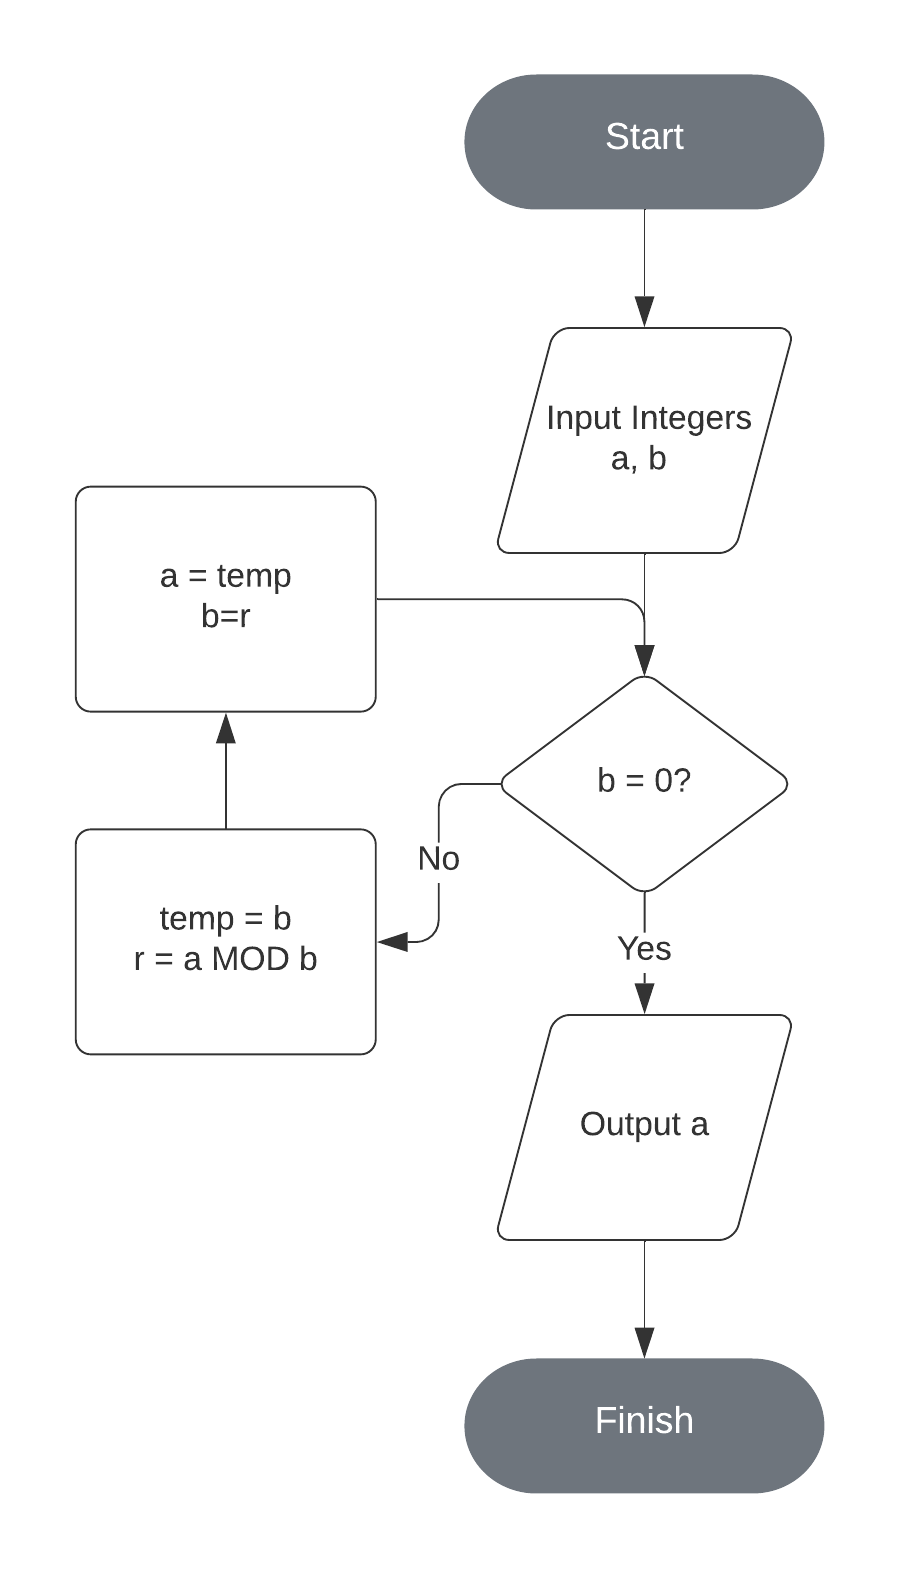
\includegraphics[width=2in]{euclidean-algorithm-flowchart}
\end{figure}

By representing the algorithm as a flowchart, we can see that it starts of by receiving two integers $a$ and $b$ as an input, and then keeps on finding the values of $n$ and $r$ from the examples, until the value of $b$ is $0$. Implementing this as code, this looping could be done using a standard \texttt{WHILE} loop, but I think that implementing this algorithm as a recursive function would be more suitable.

Implementing this algorithm in pseudocode, it would look as follows:
\begin{algorithm}
    \caption{Euclidean Algorithm Pseudocode}
    \begin{algorithmic}
        \Function{greatest\_common\_divisor}{a, b}
            \If {$b = 0$}
                \State \Return $a$
            \Else
                \State\Return\Call{greatest\_common\_divisor}{$b$, $a$ MOD $b$}
                \Comment{recursively call the function until $b = 0$}
            \EndIf
        \EndFunction
    \end{algorithmic}
\end{algorithm}

We can see from this pseudocode, the recursive nature of this algorithm.

Then writing the Euclidean Algorithm in Python:

\begin{lstlisting}
# Euclidean Algorithm
def greatest_common_divisor(a: int, b: int) -> int:
    if b == 0:
        return a
    else:
        # recursively call the function until b = 0
        return greatest_common_divisor(b, a % b)
\end{lstlisting}

This implementation of the Euclidean Algorithm in Python, is very efficient. Although it is recursive, and that can in some circumstances lead to a large amount of memory use - especially in Python - it would be relatively simple to unwind the stack at the end of the computation, because this function does not call any other functions and is relatively simple.


\subsubsection{Riemann Zeta Function}
One of the most important mathematical functions in this project is the Riemann Zeta Function. As mentioned in my analysis section, it can be defined as:
% \begin{align*}
    $$\zeta(s) = \sum^{\infty}_{n=1}\frac{1}{s^n}$$
Which can be rewritten as:
    $$\zeta(s) = \frac{1}{1-2^{1-s}} \sum_{n=0}^{\infty} \frac{1}{2^{n+1}} \sum_{k=0}^{n} (-1)^k \binom{n}{k} (k+1)^{-s}$$
% \end{align*}

This is just one of many of the ways that $\zeta(s)$ can be defined. The main advantages of this definition are that it is will allow inputs for any complex number $s$ (apart from when $s = 1$ for which $\zeta(s)$ is undefined), and that it is fast to compute.
\clearpage
Using flowcharts, we can write this function as follows:
\begin{figure}[h]
    \centering
    \caption{Zeta Function Flowchart5}
    \captionsetup{justification=centering}
    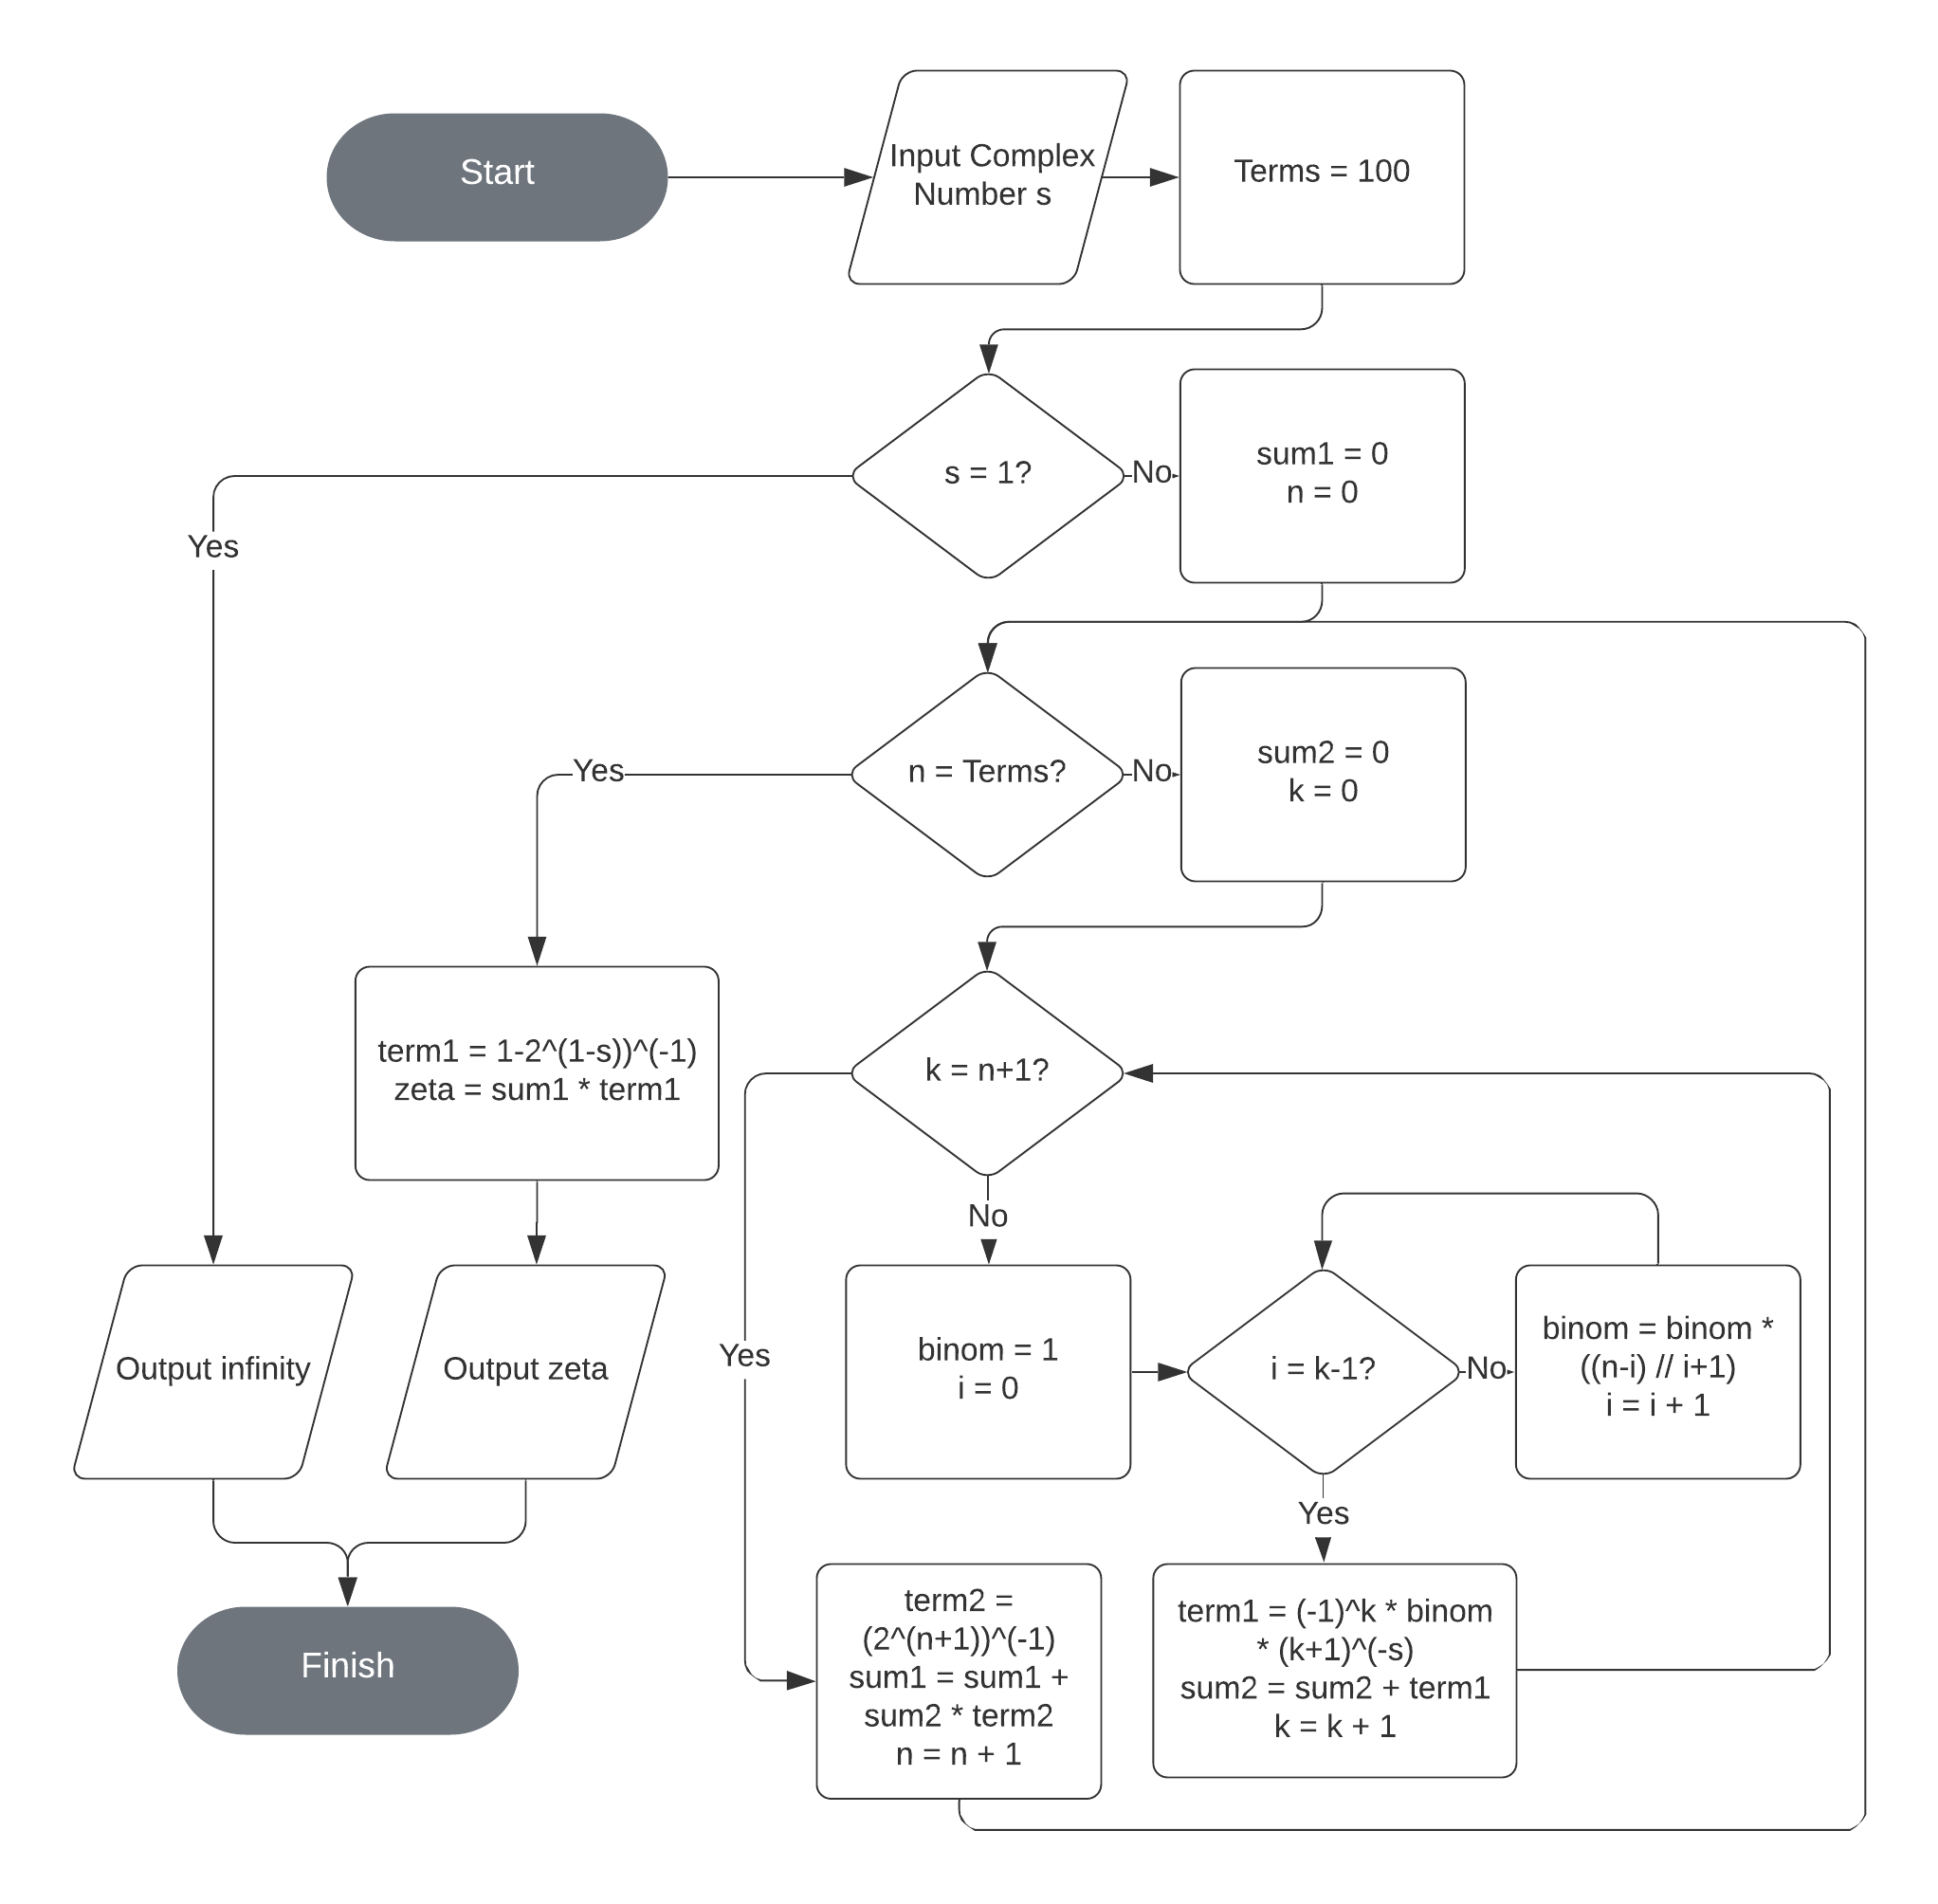
\includegraphics[width=5in]{zeta-function-flowchart-two}
\end{figure}

Unfortunately, with any computational implementation of the zeta function, it would be impossible to calculate an exact output for any given input. This is due to the fact that the zeta function, be definition is the sum of an infinite series.

It would be intractable to compute every single element in the series to be able to sum it. Because the infinite sum is convergent (except for $\zeta(1)$ which cannot be calculated), we can approximate the sum by calculating a very large number of terms in the sum, instead of an infinite amount. The number of terms we calculate in the sum is a trade-off between the time it takes to compute the function, and the accuracy of our answer.

This is what the variable \texttt{Terms}, in the flowchart, is used for. Its aim is to replace the $\infty$ in the infinite loop, such that we can still compute $\zeta(s)$ to a high degree of accuracy, with the function still being relatively time efficient.

In a sense, we are changing our definition of the zeta function, so the function that we are actually calculating is this:

$$\zeta(s) \approx \frac{1}{1-2^{1-s}} \sum_{n=0}^{\texttt{Terms}} \frac{1}{2^{n+1}} \sum_{k=0}^{n} (-1)^k \binom{n}{k} (k+1)^{-s} $$

Which is a less accurate version of the zeta function, but is actually computable.

From the flowchart, we can see how the situation where $s=1$ is handled. $\zeta(1)$ is undefined, so we would be unable to calculate this. Therefore, we have to check this special case, and if $s=1$, then the function will \texttt{OUTPUT Infinity}, otherwise, it will just continue with the rest of the function.

The rest of the function, is essentially just creating two sequences and summing them. The flowchart represents this well, it allows us to visualise the looping nature of the sequences.

We can break down our formula for the approximation of $\zeta(s)$, which will make it clear how the flowchart is designed to work.

\begin{figure}[h]
    \centering
    \caption{Decomposed Zeta Function}
    \captionsetup{justification=centering}
    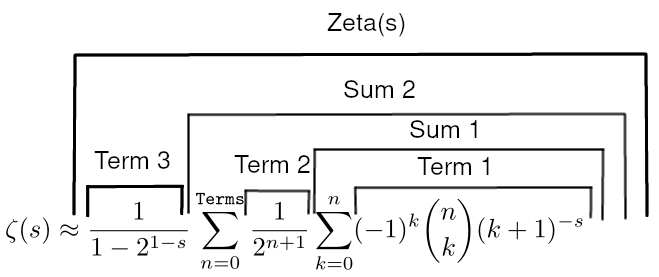
\includegraphics[scale=0.4]{zeta-approx-explained}
\end{figure}

From this image, we can see that:

$$\zeta(s) = \texttt{Term3} \cdot \texttt{Sum2}$$
Where:
$$\texttt{Sum2} = \sum \texttt{Term2} \cdot \texttt{Sum1}$$
Where:
$$\texttt{Sum1} = \sum \texttt{Term1}$$

Then, all that has to be done is replace the values of \texttt{Term1}, \texttt{Term2}, and \texttt{Term3} with their respective values, and that is essentially what is being calculated.

By applying decomposition to the function, we can now easily see how the flowchart works, and now how to implement this function by using pseudocode.
\clearpage
\begin{algorithm}[h]
    \caption{Zeta Function Pseudocode}
    \begin{algorithmic}
        \Function{zeta}{s}
            \State $TERMS \gets 100$
            \If{$s = 1$}
                \State \Return {$\infty$}
            \Else
                \For {$n \gets 0 \textbf { to } TERMS$}
                    \State $sum1 \gets 0$
                    \For {$k \gets 0 \textbf{ to } n+1$}
                        \State $sum2 \gets sum2 + (-1)^k \cdot \binom{n}{k} \cdot (k+1)^{-s}$
                    \EndFor
                    \State $sum1 \gets sum1 + sum2 \cdot \frac{1}{2^{n+1}}$
                \EndFor
                \State $constant \gets 1-2^{1-s}$
                \State \Return{$\frac{sum1}{constant}$}
            \EndIf
        \EndFunction
    \end{algorithmic}
\end{algorithm}

For sake of readability, I have omitted creating separate variables for \texttt{Term1}, \texttt{Term2}, and \texttt{Term3}. Instead, these can just be seen by the mathematical equations present in the Pseudocode.

I much prefer this representation of the function, as it easily allows you to see how the sums are implemented alongside the terms. The use of \texttt{for} loops makes it easy to see how we have a sum being calculated inside a sum.

With pseudocode, I have just been able to write the mathematical statements for readability sake, however, when implementing this as a programming language, it could look rather messy with long maths having to be written out.
One area that would need addressing when converting this pseudocode to an actual language is with the binomial coefficient, that is $\binom{n}{k}$. I have previously mentioned this in my analysis, however:

$$\binom{n}{k} = \frac{n!}{k!(n-k)!}$$

Where:
\begin{align*}
    x! &= \prod_{a=1}^x a\\
    &= x \times (x-1) \times (x-2) \times (x-3) \times \dots \times 3 \times 2 \times 1
\end{align*}
Which is itself, the product of another series.

So when calculating the zeta function in this form, we are actually having to compute, the product of 3 series , within a series, within a series. This may not seem at all time or space efficient, but these sums are a lot easier for a computer to compute than evaluating $\zeta(s)$ by its definition that is:
$$\zeta(s) = \sum^{\infty}_{n=1} \frac{1}{n^s}$$

To implement the binomial coefficient effectively, we would not be able to use it in its factorial form - this would take too long to compute. Instead, we can define the binomial coefficient another way.

If we take our equation for the definition of the binomial coefficient, and focus on the fraction of the right hand side:
$$\binom{n}{k} = \frac{n!}{k!(n-k)!}$$
We can divide the numerator and denominator by $(n-k)!$, then we have that:
$$\binom{n}{k} = \frac{\frac{n!}{(n-k)!}}{k!}$$
Then expanding the numerator:
$$\binom{n}{k} = \frac{\frac{n(n-1)(n-2)\dots(n-k+1)(n-k)(n-k-1)(n-k-2)\dots(2)(1)}{(n-k)(n-k-1)(n-k-2)\dots(2)(1)}}{k!}$$
Notice how the denominator of the numerator exactly repeats what is above it, this means that all of these terms can cancel, such that we are left with:
$$\binom{n}{k} = \frac{n(n-1)(n-2)\dots(n-k+2)(n-k+1)}{k!}$$
Which can be rewritten as:
$$\binom{n}{k} = \frac{n^{\underline{k}}}{k!}$$
Where $n^{\underline{k}}$ is known as a falling factorial power and is defined as:

\begin{align*}
    n^{\underline{k}} &= n(n-1)(n-2) \dots (n-k+1)\\
    &= \prod_{x=1}^k (n - (x - 1))\\
    &= \prod_{x=1}^{k-1} (n - x)
\end{align*}

So looking back at how to use this to calculate the binomial coefficient, we can say that:
\begin{align*}
    \binom{n}{k} &= \frac{n!}{k!(n-k)!}\\
    &= \frac{n^{\underline{k}}}{k!}\\
    &= \frac{n(n-1)(n-2)\dots (n-(k-1))}{k(k-1)(k-2) \dots 1}\\
    &= \prod^k_{i=1} \frac{n+1-i}{i}\\
    &= \prod^{k-1}_{i=0} \frac{n-i}{i+1}
\end{align*}

We now have a function, that we can be called from inside the zeta function, in order to calculate the appropriate binomial coefficient.

Implementing the binomial coefficient function as pseudocode would look as follows:

\begin{algorithm}[ht]
    \caption{Binomial Coefficient Pseudocode}
    \begin{algorithmic}
        \Function{binom}{$n$, $k$}
            \State $b \gets 1$
            \For {$i \gets 0 \textbf { to } k$}
                \State $b = b \times \frac{n-i}{i+1}$
            \EndFor
            \State \Return $b$
        \EndFunction
    \end{algorithmic}
\end{algorithm}

Rewriting our definition of the zeta function, with this new way of calculating the binomial coefficient, we can now say that:

$$\zeta(s) \approx \frac{1}{1-2^{1-s}} \sum_{n=0}^{\texttt{Terms}} \left( \frac{1}{2^{n+1}} \sum_{k=0}^{n} \left( (-1)^k \left(\prod^{k-1}_{i=0} \frac{n-i}{i+1} \right) (k+1)^{-s} \right) \right)$$

% \clearpage
We are then able to convert both the Zeta Function Pseudocode and the Binomial Coefficient Pseudocode into Python code
\begin{lstlisting}
# Binomial Coefficient
# \binom{n}{k} = \prod^{k-1}_{i=0} \frac{n-i}{i+1}
def binom(n, k):
    v = 1
    for i in range(k):
        v *= (n - i) / (i + 1)
    return v

# Global Zeta Function
# \zeta(s) \approx \frac{1}{1-2^{1-s}} \sum_{n=0}^{\texttt{TERMS}} \left( \frac{1}{2^{n+1}} \sum_{k=0}^{n} \left( (-1)^k \left(\prod^{k-1}_{i=0} \frac{n-i}{i+1} \right) (k+1)^{-s} \right) \right)
def zeta(s, TERMS=100):
    if s == 1:
        return float('inf')
    # \sum_{n=0}^{\texttt{TERMS}} \left( \frac{1}{2^{n+1}} \sum_{k=0}^{n} \left( (-1)^k \left(\prod^{k-1}_{i=0} \frac{n-i}{i+1} \right) (k+1)^{-s} \right) \right)
    sum1 = 0
    for n in range(TERMS):
        # \sum_{k=0}^{n} \left( (-1)^k  \binom{n}{k} (k+1)^{-s} \right)
        sum2 = 0
        for k in range(n + 1):
            sum2 += (-1) ** k * binom(n, k) * (k + 1) ** (-s)
        sum1 += sum2 * (1 / (2 ** (n+1)))
    return sum1 * (1 / (1 - 2 ** (1 - s)))
\end{lstlisting}

Now we have a very efficient program that can be used to calculate any value of $\zeta(s)$.

This function will be used extensively throughout my technical solution to plot graphs, find data points and to try to help provide some proof for the Riemann Hypothesis.

\subsubsection{Circular Queue}
For parts of my project, I will require a FIFO Queue Data Structure. I will be implementing this using a circular queue. This data structure will be a class, that has a set of methods that manipulate the data in the queue. The first of these methods will be the procedure that is called to initialise the queue. When an instance of the Queue class is created, the Queue class will require an input\_queue parameter, which will have the beginning items of the queue in it. Potentially also a max\_size parameter could be used if a static data structure is wanted by the user rather than a dynamic one. When the class is initialised, a size variable will need to be created to keep track of the current length of the queue, as well as a max\_size. The queue will then have to be created with the input queue at the front, and any remaining spaces left in the queue will have to be filled in with some filler character. Variables for the front and rear pointers of the queue will then need to be created.

One of the methods used in this implementation of a Circular Queue will be the is\_full function. If the size of the queue is equal to it's maximum size, then the function will return true, otherwise it will return false.

Another method is the function is\_empty. If the size of the queue is 0, then the function will return true, otherwise it will return false.

As well as this is the enQueue method, which will take a parameter of an item. In this procedure, the item is appended to the rear of the circular queue. This procedure can only be run if the queue is not already full, if it is full, then an error will be thrown. If the queue is not full, then the element in the queue that is at the position of the rear pointer will be set equal to the item that is being enqueued. The rear pointer will then need to be incremented. The rear pointer is increased by 1, but if this value goes above the max\_size of the queue, then it will need to be set to 0. For this the mod function can be used. The variable for the size of the list will then need to be incremented by one.

Similar to this is deQueue, where an item is removed from the front of the queue and it's value is returned. This function can only be run if the queue is not already empty, otherwise an error will be thrown. The variable item will be used to hold the value of the element in the queue where it's index is equal to the front pointer. The element at this position can then be set to some blank / placeholder value. This is not necessary for computation but helps with readability when printing the queue. The front pointer will then need to be incremented by one, but be modded in a similar way to the rear queue during an enQueue. The size variable will need to be decremented by one and the item variable will be returned.

The flowcharts for each of these subroutines looks as follows:

\begin{figure}[ht]
    \centering
    \begin{subfigure}{.5\textwidth}
        \centering
        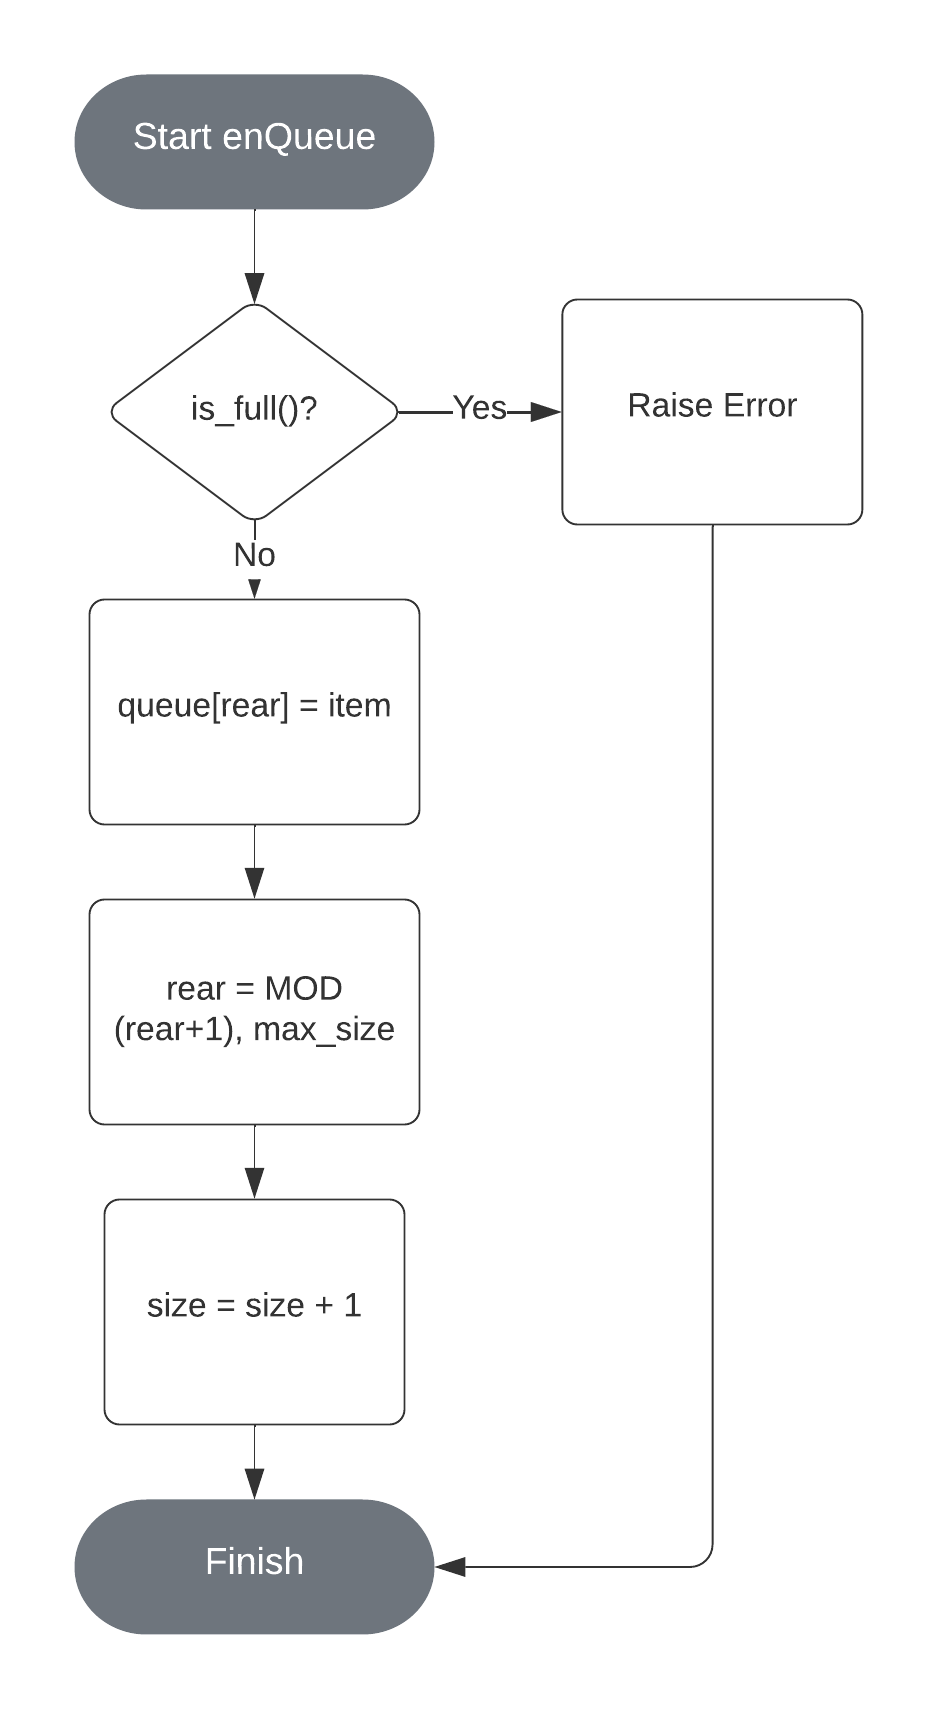
\includegraphics[width=.8\linewidth]{enQueue-circular-queue-flowchart}
        \caption{enQueue method flowchart}
    \end{subfigure}%
    \begin{subfigure}{.5\textwidth}
      \centering
      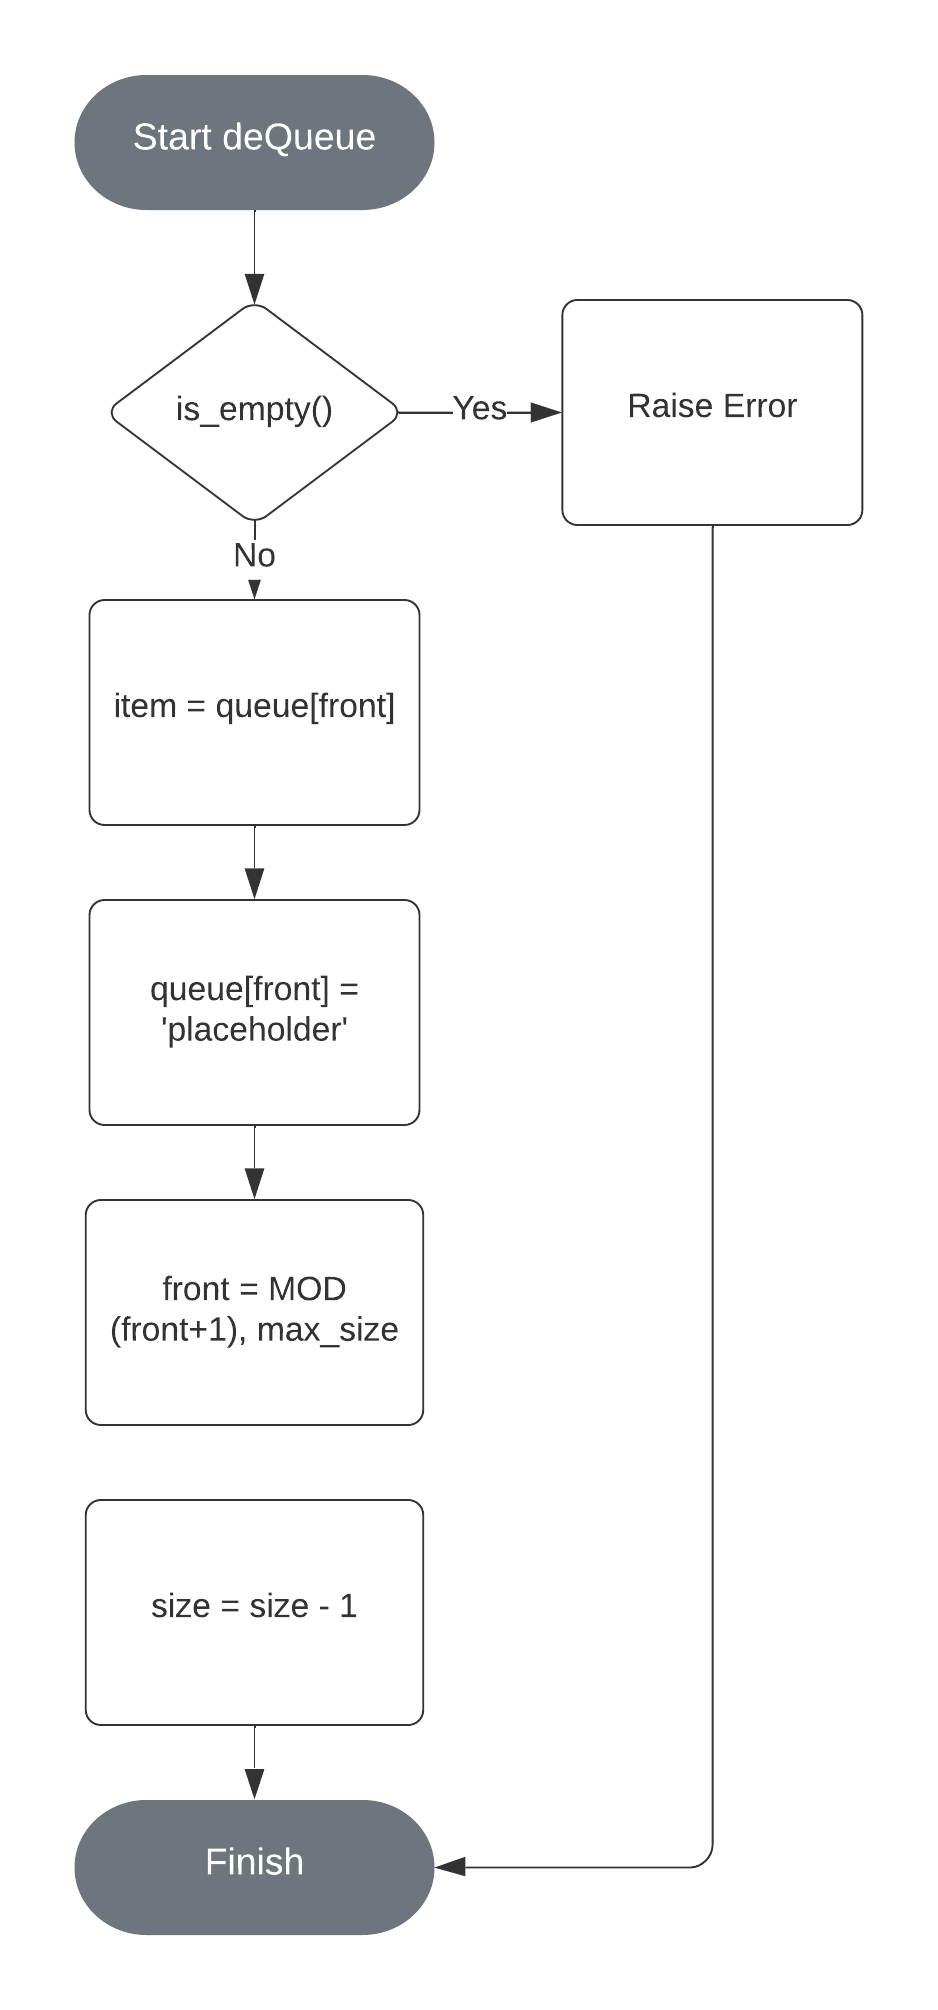
\includegraphics[width=.8\linewidth]{deQueue-circular-queue-flowchart}
        \caption{deQueue method flowchart}
    \end{subfigure}

    \begin{subfigure}{.5\textwidth}
        \centering
        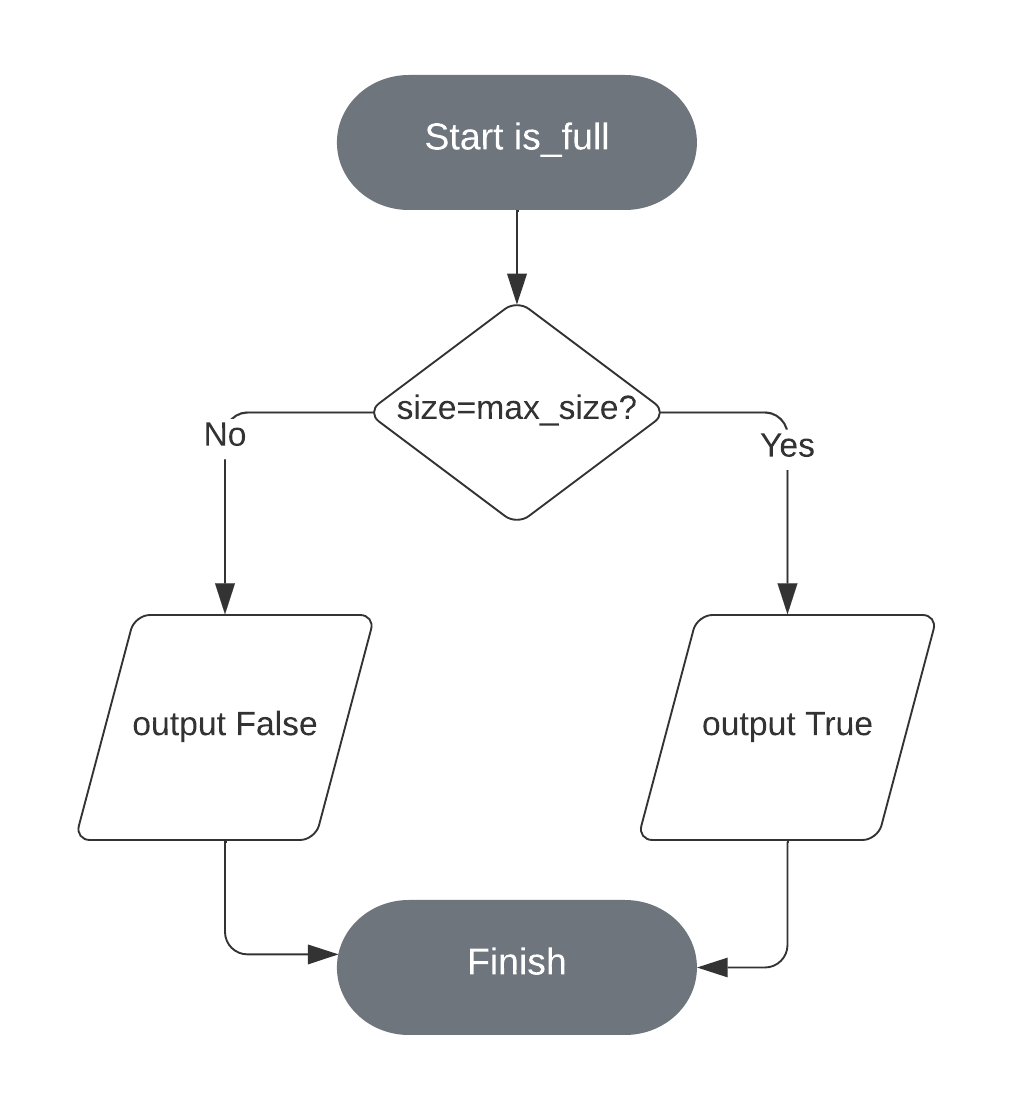
\includegraphics[width=.8\linewidth]{is-full-circular-queue-flowchart}
        \caption{is\_full method flowchart}
    \end{subfigure}%
    \begin{subfigure}{.5\textwidth}
      \centering
      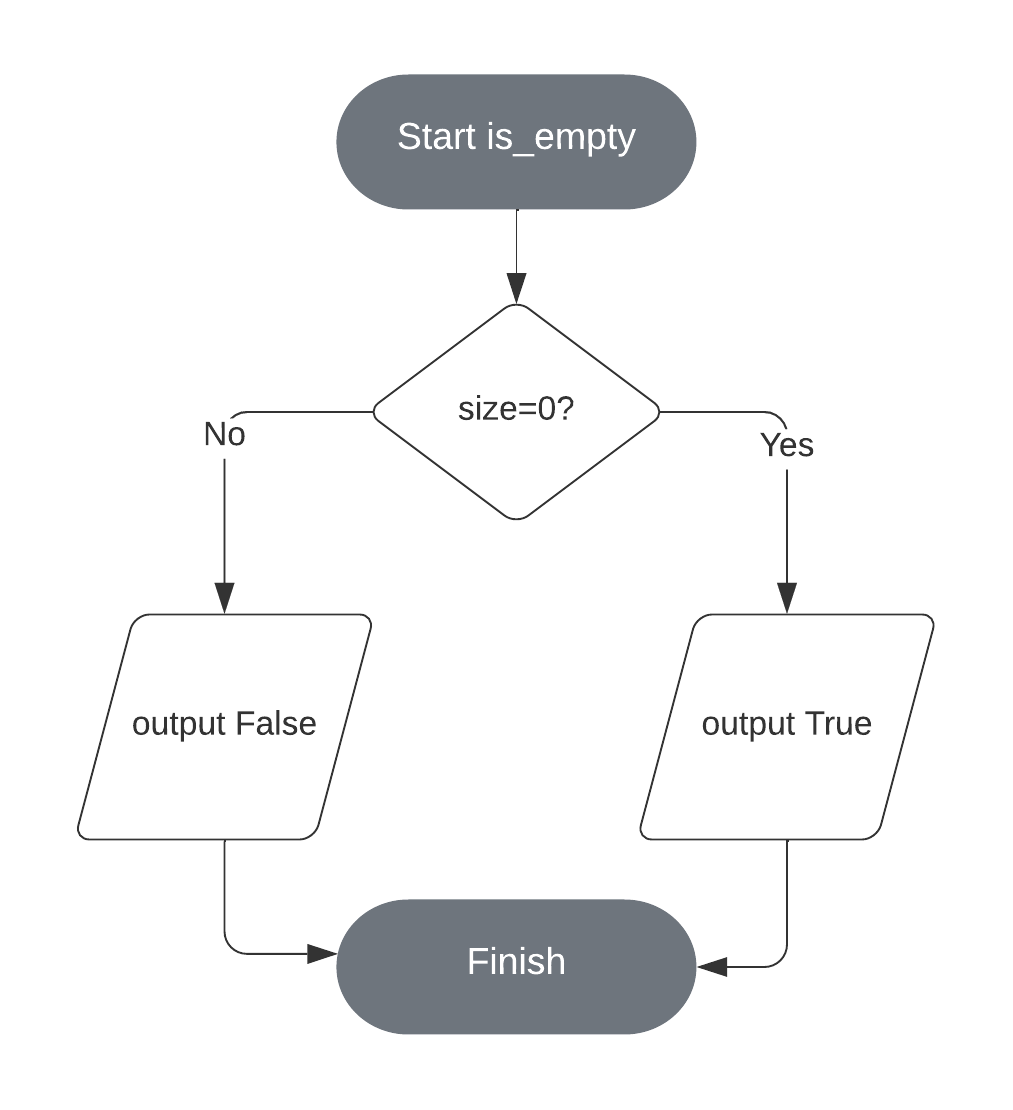
\includegraphics[width=.8\linewidth]{is-empty-circular-queue-flowchart}
        \caption{is\_empty method flowchart}
    \end{subfigure}
    \caption{Flowcharts for Circular Queue Methods}
\end{figure}

\clearpage

Implementing the circular queue in pseudocode looks as follows:
\algblockdefx[Name]{Class}{EndClass}%
[2][Unknown]{\textbf{class} #1(#2)}%
    {\textbf{end class}}
\algblockdefx[Name]{PubFunc}{EndPubFunc}%
[2][Unknown]{\textbf{public function} #1(#2)}%
    {\textbf{end function}}
\algblockdefx[Name]{PubProc}{EndPubProc}%
[2][Unknown]{\textbf{public prodecure} #1(#2)}%
    {\textbf{end procedure}}

\begin{algorithm}[ht]
    \caption{Circular Queue Pseudocode}
    \begin{algorithmic} [1]
        \Class[CIRCULAR QUEUE]{input\_queue, max\_size}
        \PubFunc[\_\_INIT\_\_]{self, input\_queue, max\_size}
                \State{$size \gets \textbf{ length } input\_queue$}
                \State{$front \gets 0$}
                \State{$rear \gets size$}
                \If{$size > max\_size$}
                    \State \Return Error
                \Else
                    \State{$blanks \gets list()$}
                    \State{$no\_of\_blanks \gets max\_size-size$}
                    \For {$i \gets 0 \textbf{ to } no\_of\_blanks$}
                        \State{$blanks = blanks + 'placeholder'$}
                    \EndFor
                    \State{$queue \gets input\_queue + blanks$}
                \EndIf
            \EndPubFunc\\

            \PubProc[ENQUEUE]{item}
                \If{$\text{IS\_FULL()} = True$}
                    \State {\Return Error}
                \Else
                    \State{$queue[rear] \gets item$}
                    \State{$rear \gets \textbf{ mod } rear+1, max\_size$}
                    \State{$size \gets size + 1$}
                \EndIf
            \EndPubProc

            \algstore{circular-queue}
    \end{algorithmic}
\end{algorithm}
\clearpage

\begin{algorithm}[ht]
    \caption{Circular Queue Pseudocode Continued}
    \begin{algorithmic} [1]
            \algrestore{circular-queue}

            \PubFunc[DEQUEUE]{item}
                \If{$\text{IS\_EMPTY()} = True$}
                    \State {\Return Error}
                \Else
                    \State{$item \gets queue[front]$}
                    \State{$queue[front] \gets 'placeholder'$}
                    \State{$front \gets \textbf{ mod } front+1,  max\_size$}
                    \State{$size \gets size - 1$}
                    \State \Return $item$
                \EndIf
            \EndPubFunc\\

            \PubFunc[IS\_FULL]{}
                \If{$size = max\_size$}
                    \State {\Return $True$}
                \Else
                    \State{\Return $False$}
                \EndIf
            \EndPubFunc\\

            \PubFunc[IS\_EMPTY]{}
                \If{$size = 0$}
                    \State {\Return $True$}
                \Else
                    \State{\Return $False$}
                \EndIf
            \EndPubFunc
        \EndClass
    \end{algorithmic}
\end{algorithm}

And then converting this pseudocode to python it will look as follows:

\begin{lstlisting}
class Queue:

    """
    Implementation of a circular queue

    Contains the subroutines:
        - enQueue
        - deQueue
        - is_full
        - is_empty

    """







    def __init__(self, input_queue, **kwargs):
        self.input_queue = input_queue
        self.size = len(self.input_queue)
        self.front = 0
        self.rear = len(self.input_queue)
        if 'max_size' in kwargs.keys():
            self.max_size = kwargs['max_size']
        else:
            self.max_size = len(self.input_queue)
        if self.size > self.max_size:
            raise IndexError("max_size must be greater than or equal to the size of the input queue")
        else:
            self.blanks = [False for i in range(self.max_size - self.size)]
            self.queue = self.input_queue + self.blanks

    def enQueue(self, item):
        """Appends an item to the rear of the circular queue"""
        if self.is_full():
            raise IndexError("Tried to enqueue to a full queue")
        else:
            self.queue[self.rear] = item
            self.rear = (self.rear+1) % self.max_size
            self.size += 1

    def deQueue(self):
        """Remove and return the value at the front of the circular queue"""
        if self.is_empty():
            raise IndexError("Tried to dequeue from an empty queue")
        else:
            item = self.queue[self.front]
            self.queue[self.front] = False
            self.front = (self.front+1) % self.max_size
            self.size -= 1
            return item

    def is_full(self):
        """Check if the circular queue is full"""
        return self.size == self.max_size

    def is_empty(self):
        """Check if the circular queue is empty"""
        return self.size == 0
\end{lstlisting}

\clearpage
\subsubsection{Binary Insertion Sort}
Throughout the program I will be required to sort sets of data. To sort the data, I will be using a binary insertion sort algorithm, due to it's low time and space complexity. Although not too efficient on large data sets, I should only be handling relatively small data sets during this program so the binary insertion sort should suffice for all sorting in the program.

A normal insertion sort works by having a queue which will originally contain each element in the original array. The item at the front of the queue will be removed from the queue and be placed in an array containing the elements in sorted order. When an element is taken from the queue and put in the sorted array, it is put in a position such that the elements either side of it are lower and higher than it. Once evert element has been moved from the queue to it's correct position in the sorted list, the sorted list will contain every element that was in the original array but in sorted order.

A binary insertion sort is a variation of the normal insertion sort, but instead it uses a binary search, rather than a linear search to find the position that the element will go in the sorted list. This improves the time complexity of the program from O(n) to O(log n).

In pseudocode, the algorithm for a binary insertion sort looks as follow:

\begin{figure}[h]
    \centering
    \captionsetup{justification=centering}
    \caption{Binary Insertion Sort Flowchart}
    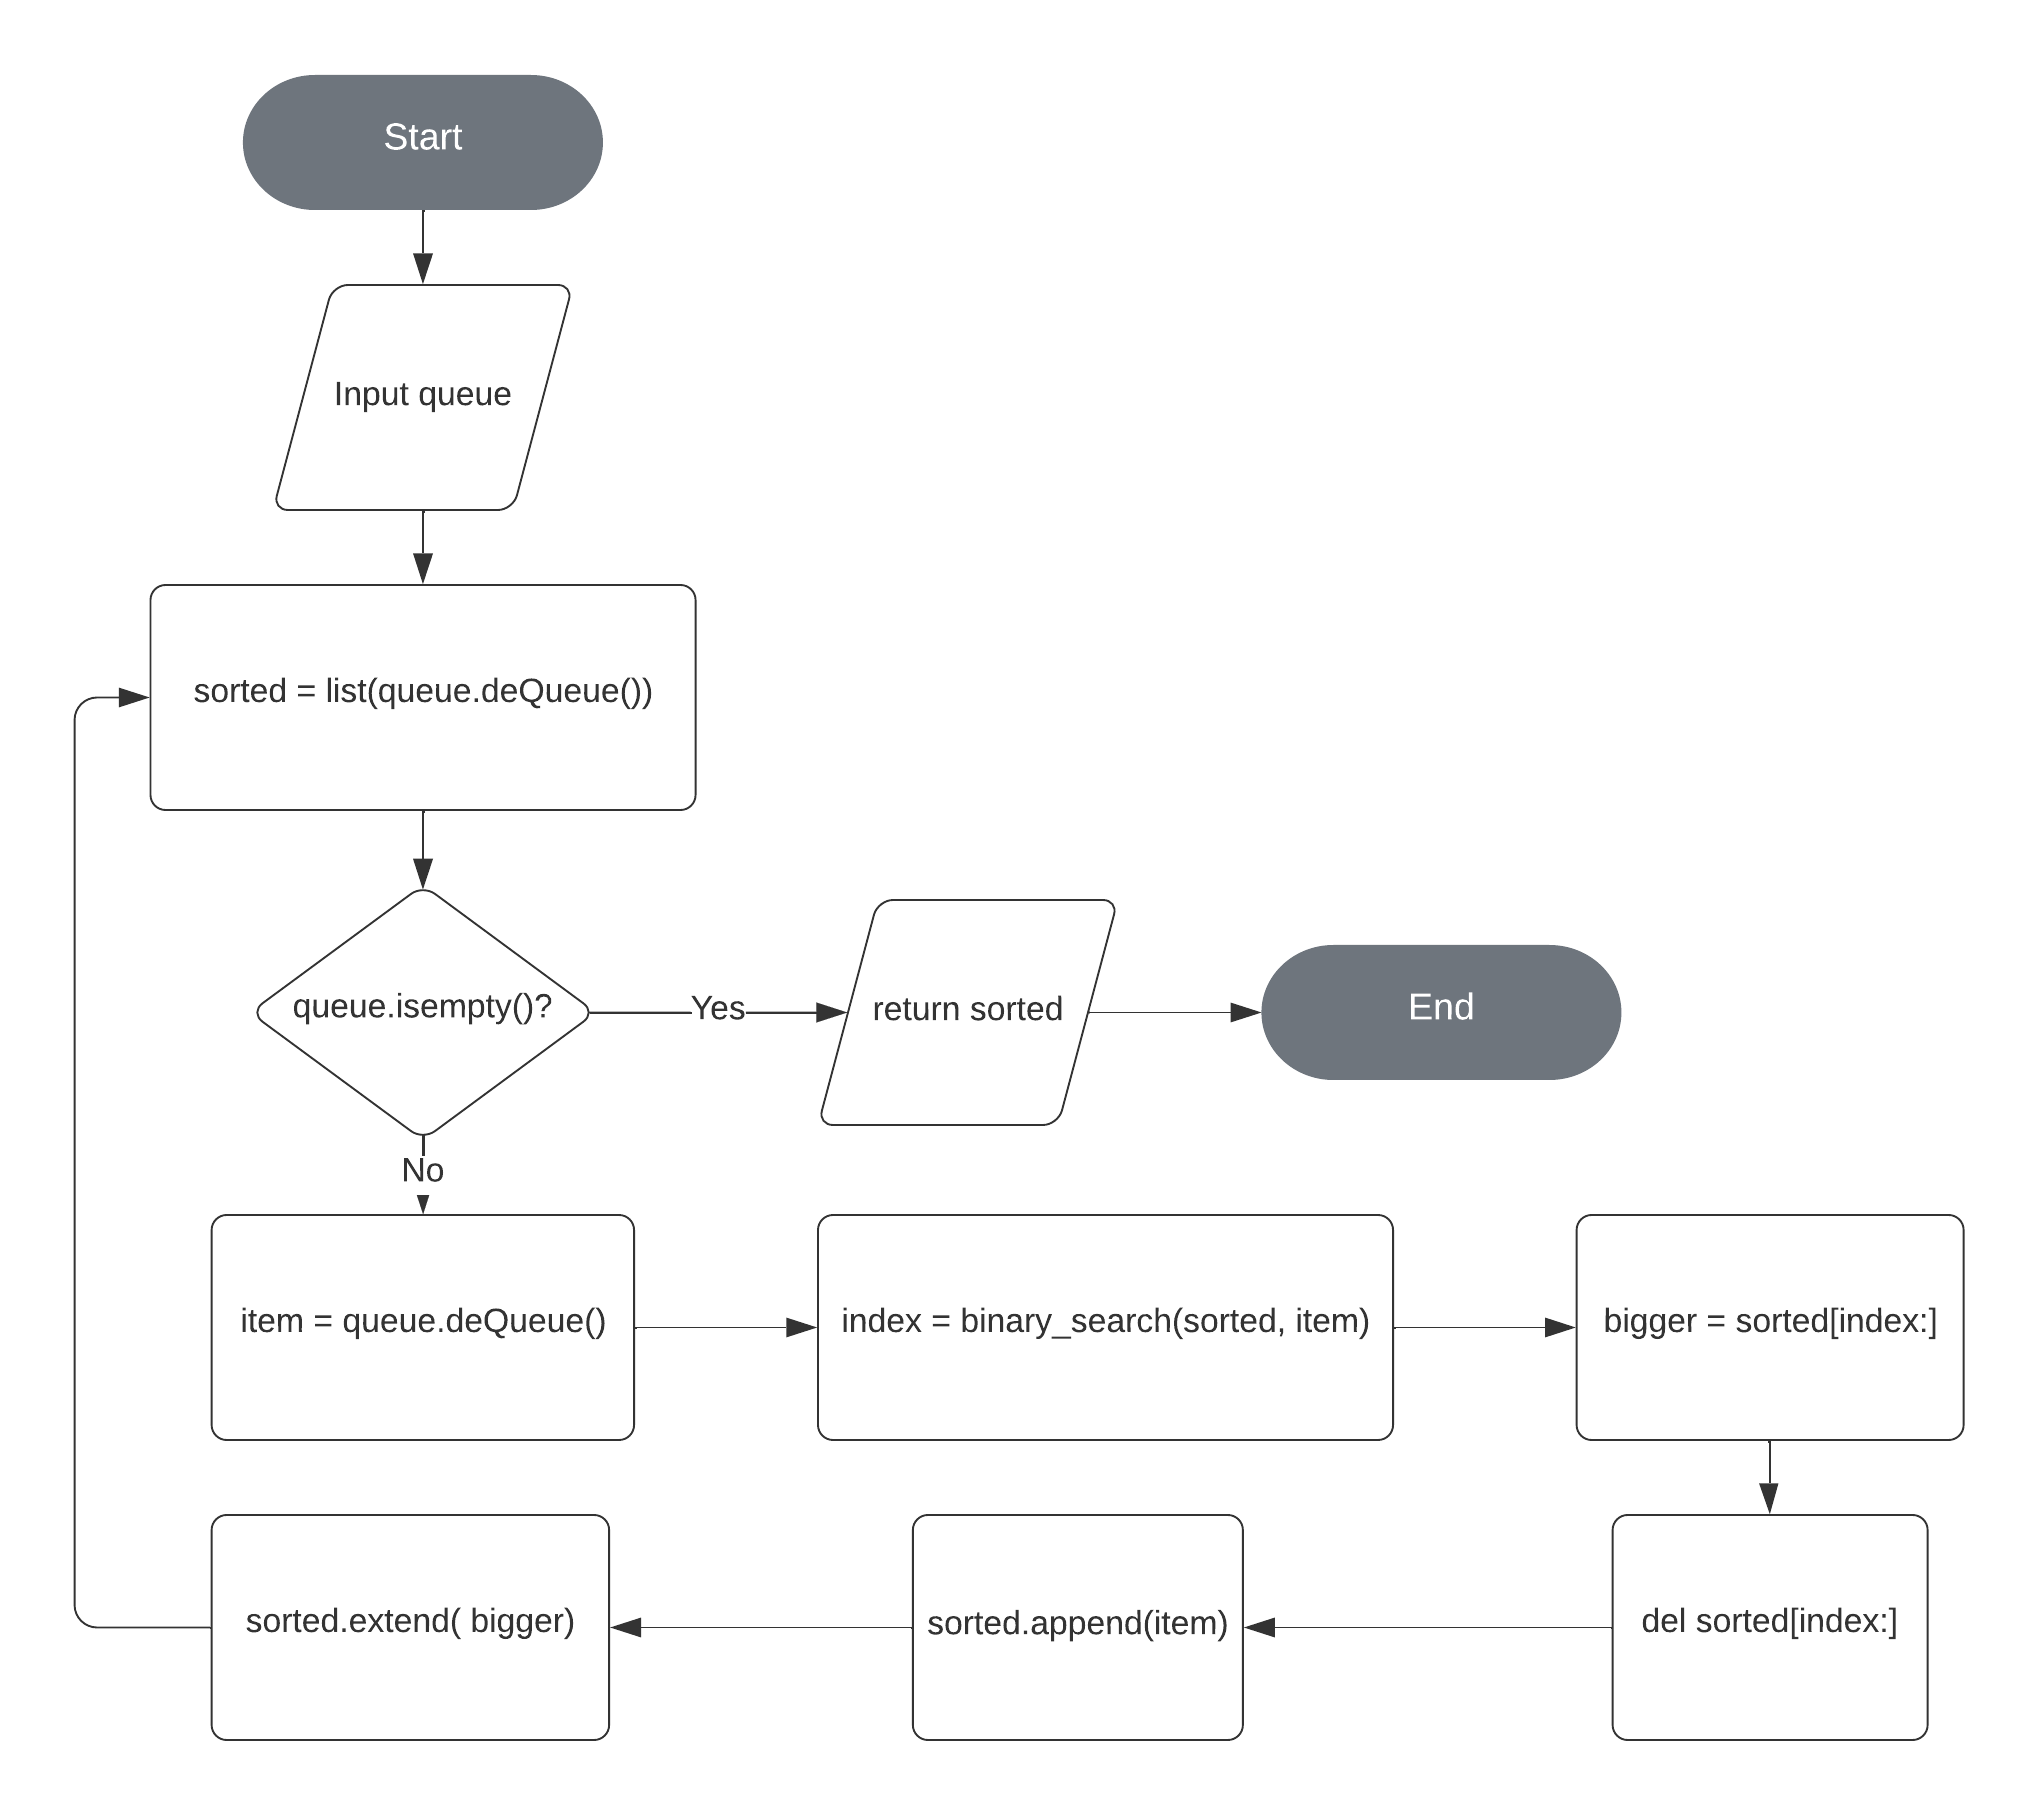
\includegraphics[width=6in]{binary-insertion-sort-flowchart}
\end{figure}
\clearpage
This algorithm written in pseudocode looks as follows:

\begin{algorithm}[ht]
    \caption{Binary Insertion Sort Pseudocode}
    \begin{algorithmic} [1]
        \Function{binary\_insertion\_sort}{data}
            \State{$queue = \text{Queue}(data)$}
            \State{$sorted \gets list()$}
            \State{$sorted \gets sorted + \text{queue.DEQUEUE()}$}
            \While{\textbf{ not } \text{queue.IS\_EMPTY()}}
                \State{$index \gets \text{binary\_search}(sorted, item)$}
                \State{$bigger \gets sorted[index:]$}
                \State{$\textbf{delete} \text{ } sorted[index:]$}
            \EndWhile
            \State{\Return $sorted$}
        \EndFunction
    \end{algorithmic}
\end{algorithm}

And then writing the algorithm in python:

\begin{lstlisting}
def binary_insertion_sort(data, descending=False):

    """
    Sorts a list of data into ascending order using a binary insertion sort
    """

    try:
        array = list(map(float, data ))
    except ValueError:
        array = data
    queue = Queue(array)
    sorted = [queue.deQueue()]
    while not queue.is_empty():
        item = queue.deQueue()
        index = binary_search(sorted, item)
        bigger = sorted[index:]
        del sorted[index:]
        sorted.append(item)
        sorted.extend(bigger)
    if not descending:
        return sorted
    else:
        return sorted[::-1]
\end{lstlisting}

This python variation of the binary insertion sort algorithm also includes an option to return the sorted list in descending order, as well as the default ascending order.
% \subsection{Data Structure Design}

\clearpage

\subsection{File Structure}

In this section, I will showcase the full planned File Structure for the program.

\begin{itemize}
    \item \textbf{program}
    \begin{itemize}
        \item \textbf{user\_interface}
        \begin{itemize}
            \item \textbf{introduction\_ui}
            \begin{itemize}
                \item \_\_init\_\_.py
                \item Various python files for the introduction UI
            \end{itemize}
            \item \textbf{ivnestigation\_ui}
            \begin{itemize}
                \item \_\_init\_\_.py
                \item Various python files for the investigation UI
            \end{itemize}
            \item \textbf{login\_ui}
            \begin{itemize}
                \item \_\_init\_\_.py
                \item Various python files for the login UI
            \end{itemize}
            \item \textbf{notes\_ui}
            \begin{itemize}
                \item \_\_init\_\_.py
                \item Various python files for the notes UI
            \end{itemize}
            \item \textbf{summary\_ui}
            \begin{itemize}
                \item \_\_init\_\_.py
                \item Various python files for the summary UI
            \end{itemize}
            \item \textbf{tutorial\_ui}
            \begin{itemize}
                \item \_\_init\_\_.py
                \item Various python files for the tutorial UI
            \end{itemize}
            \item \_\_init\_\_.py
            \item main\_menu.py
            \item mat\_plot.py
            \item progress.py
        \end{itemize}
        \item \textbf{utils}
        \begin{itemize}
            \item \_\_init\_\_.py
            \item computational\_functions.py
            \item cryptography\_functions.py
            \item database\_functions.py
            \item email\_functions.py
            \item file\_handling.py
            \item mathematical\_functions.py
            \item number\_systems.py
            \item screen\_design.py
            \item user.py
        \end{itemize}
        \item \_\_init\_\_.py
        \item introduction\_section.py
        \item investigation\_section.py
        \item login\_section.py
        \item main\_section.py
        \item notes.py
        \item summary\_section.py
        \item tutorial\_section.py
    \end{itemize}
    \item main.py
\end{itemize}

As you can see from this file structure list, there will be many python files involved in my project. I have sufficiently modularised each file, and each directory to make imports of functions across files as streamlined as possible. main.py will be the main entry point in the program, and will run the code located in the \textbf{program} directory. The \textbf{user\_interface} directory will contain a large amount of files, however these files are somewhat unimportant when it comes to the complexity and meeting my objectives of the project. Inside the \textbf{user\_interface} directory is a directory for the UI's for each of the main sections in the program. Inside each of these directories is the code required to run the user interface for the page.

Each of these different UI sections will then it's own python file in the \textbf{program} directory, which is used to display the UI at the correct point, and allow buttons, tabs, and other interactive features to work.

The more interesting and complex code can be found in the \textbf{utils} directory. Inside this directory are key algorithms, functions, procedures, and classes that are used throughout the program.

\clearpage

\subsection{HCI and Screen Designs}
Throughout this section, I will be creating initial designs for my screen pages used throughout the program.

Each page will have a consistent structure and layout, such that it will not be confusing for a user to be able to use and navigate page.

I will not be showing the design of every page used - because they are largely similar - I will instead just be showcasing and explaining some of the designs for my most important or unique parts of the project.

\subsubsection{Generic Template}
The consistent design for my user interface will follow the following template design.

\begin{figure}[ht]
    \centering
    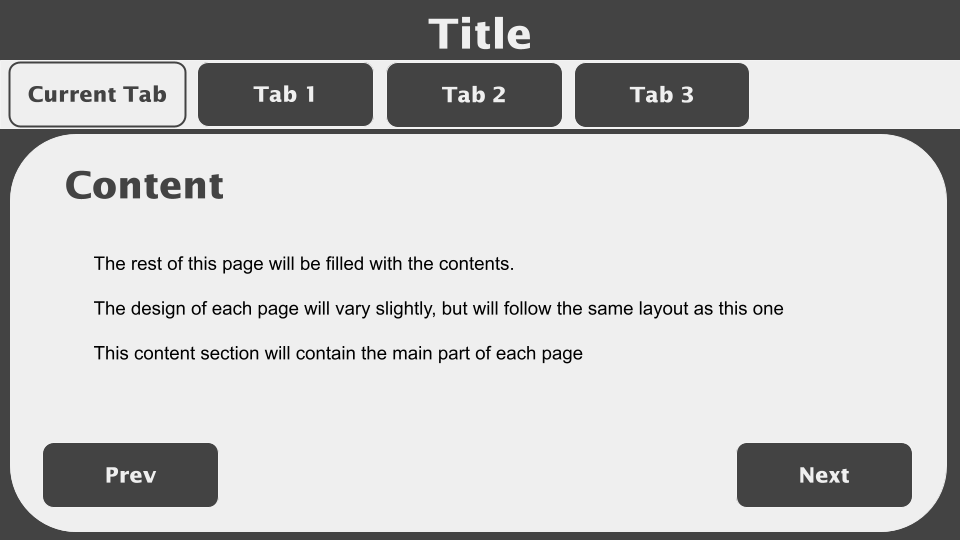
\includegraphics[scale=0.3]{template-screen-design}
    \caption{Generic Screen Design}
\end{figure}

At the top of the page is the title. This is there to show the user which page they are on.

Below this, is the tab line. Each tab on the bar  will be a clickable button, that will take the user to a different screen. The user will be able to go through the tabs in whichever order they please, which may not necessarily be in the order they are arranged; although the program will be designed such that the next tab will follow on from the previous one.

The section with the title 'Content' will show the main part of each page. For example, if the page was showing a graph plot, it will be displayed in this section.

At the bottom of the page, are the previous and next buttons, this will display the previous and next tabs respectively. These button will allow for the user to navigate between each of the pages more easily.

\clearpage
\subsubsection{Main Menu Screen Design}

The main menu is the main entry point for the user into the program. This will be what the user first sees when they launch the program, and will display all of the possible menu options for them.

It is important that this page looks visually appealing, but is also very functional and allows for efficient traversal between screen pages.

\begin{figure}[ht]
    \centering
    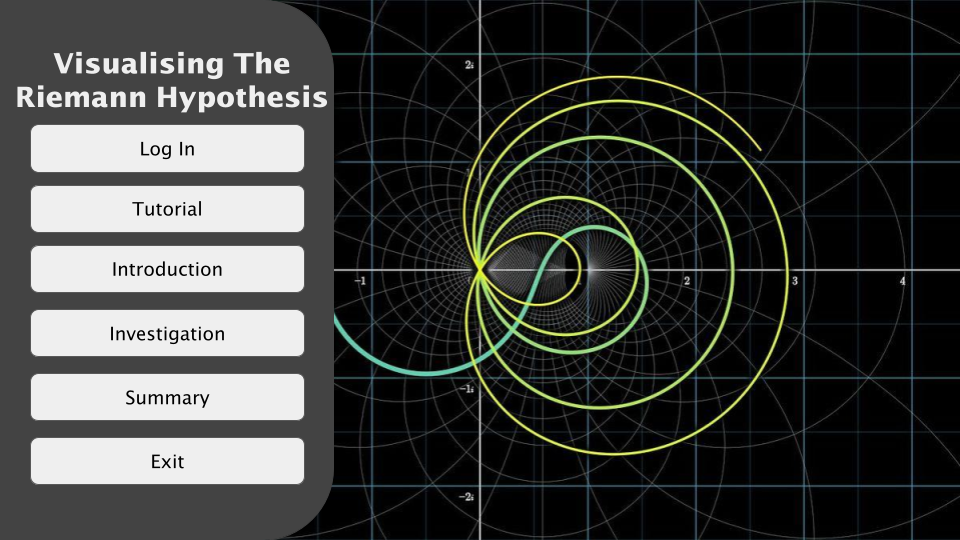
\includegraphics[scale=0.2]{main-menu-screen-design}
    \caption{Main Menu Screen Design}
\end{figure}

On the left hand side, is displayed a menu of all of the sections of the program that the user is able to navigate to. It is recommended that the user goes through them in the order shows, however, they will be able to navigate the sections however they please.

Selecting each menu option will show a new page for that respective section, and close the main menu page. When the user is finished with that section, they will then be sent back to the main menu screen.

If the user chooses to log in, the their username will shown on the main menu screen, as demonstrated in the figure below.

\begin{figure}[h]
    \centering
    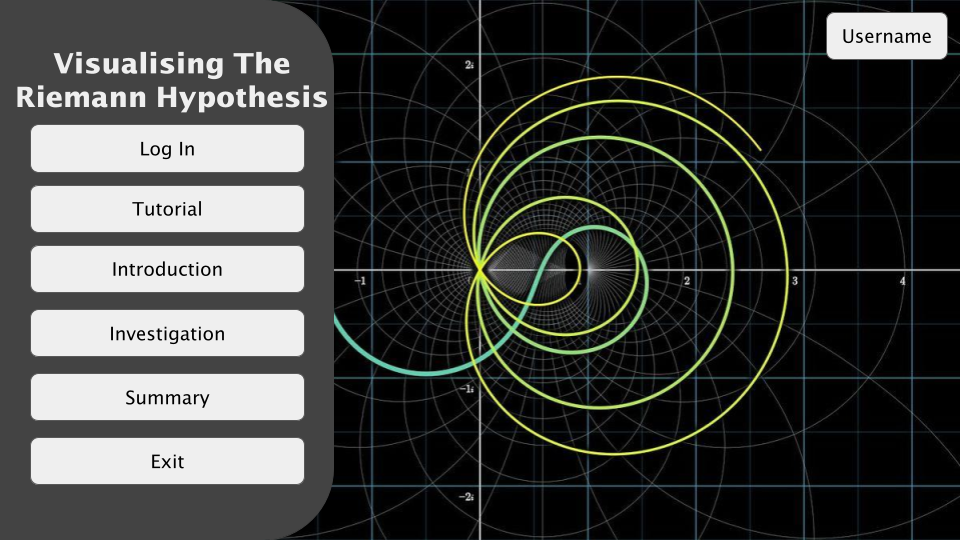
\includegraphics[scale=0.2]{main-menu-logged-in-screen-design}
    \caption{Logged In Main Menu Screen Design}
\end{figure}

\clearpage

\subsubsection{Login Screen Design}

\begin{figure}[ht]
    \centering
    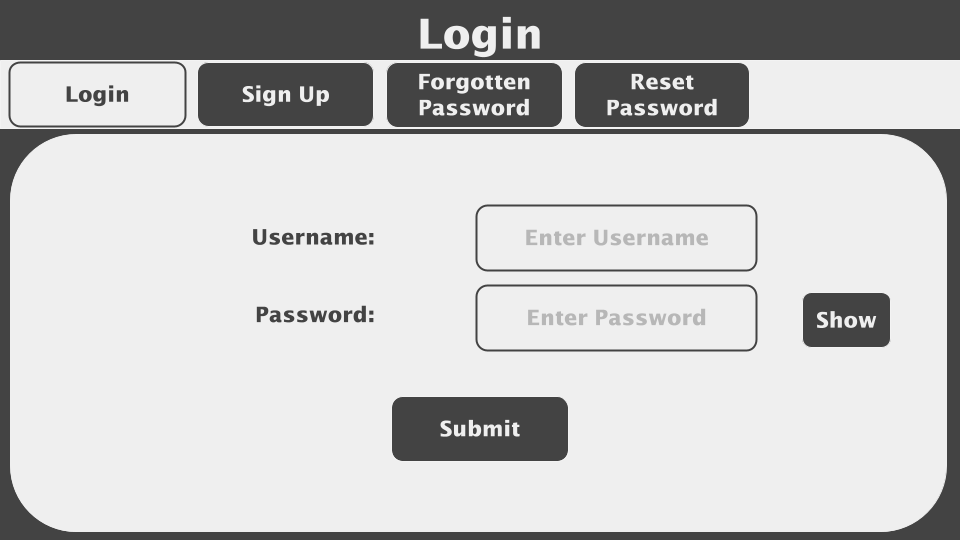
\includegraphics[scale=0.3]{login-screen-design}
    \caption{Login Screen Design}
\end{figure}

From the figure above, we can see a prototype design for the Login Page.
On the tab bar are the different options for the user. The login screen starts on the page that will be most-used, that is to be able to sign in to the program. However, the tab bar means that if a user wants to create an account, or reset their password, then they have the option there.

The user's password will not be visible when they type it in for security reasons, but in case they want to see what the have typed, then there is a show button for them.

If the user incorrectly types their username/password, then an error message will be displayed just above the submit button.

The submit button will take the user's input for their username and password, and check it against the stored values in the database. If they are incorrect, the error will be displayed, if the credentials are correct, then the user will be taken back to the main menu, and it will display their username, showing that they are logged in.

The user will then be able to go to any part of the program they wish, and have their data saved for the next time they want to use the program.

\clearpage

\subsubsection{Graph Plots Screen Design}

As part of the investigation section of the project, the user will have the opportunity to interact with various graphs. An example of how this would look is shown in the figure below.

\begin{figure}[ht]
    \centering
    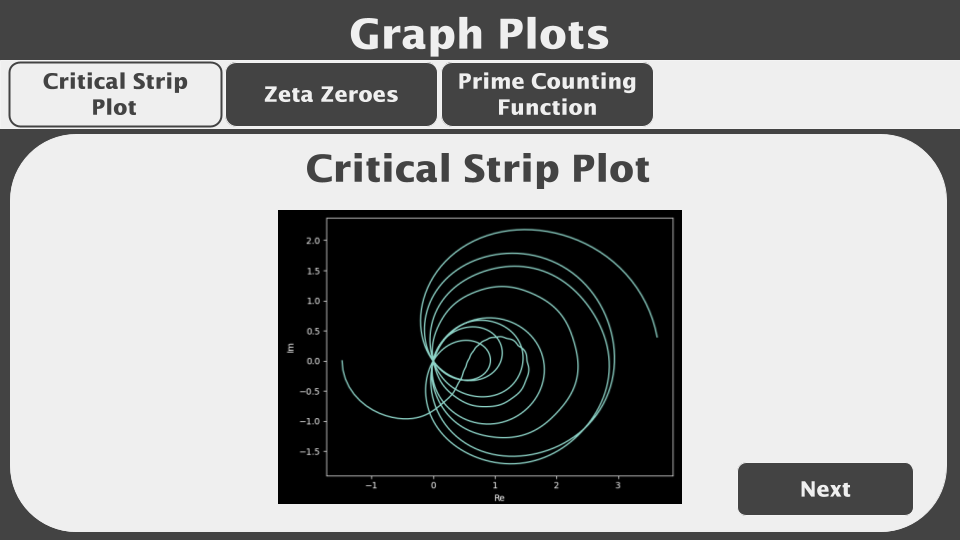
\includegraphics[scale=0.18]{graph-plots-screen-design}
    \caption{Graph Plot Screen Design}
\end{figure}

The graph will be animated, such that it updates in real time as the user is looking at it. The user will also be able to change input values into the graph plots.

\subsubsection{Calculator Screen Design}

Another part of the investigation section will be where the user can calculate values of the zeta function. The basic version will be where the user can enter a single input value, and an output value is calculated.

A more advanced version is where the user defines a range of value for the input, by given a start value, a stop value and a step value for the difference between the values.

\begin{figure}[h]
    \centering
    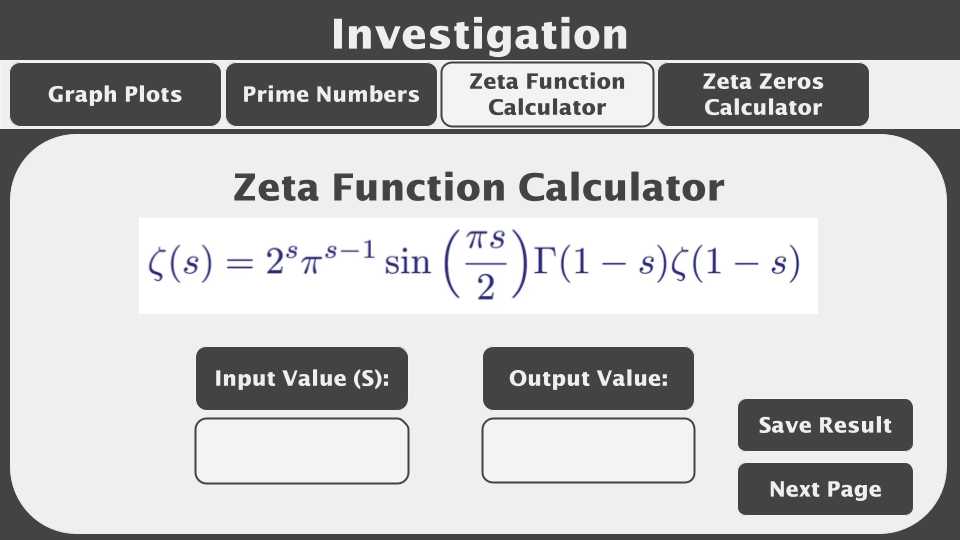
\includegraphics[scale=0.18]{zeta-function-calculator-screen-design}
    \caption{Zeta Function Calculator Screen Design}
\end{figure}

The user will then be able to store the output values from this calculator in a database. The database will contain values of zeta that every user who uses the program calculates, and each input output pair calculated will be stored with the user who found out the value, then there will be a leaderboard of who has calculated the most values for the zeta function.


\clearpage
\section{Technical Solution}

\subsection{Program Re-design}
While creating my solution to the problem, I realised that my initial design was lacking in some areas, and a lot if it needs to be updated.

\subsubsection{Database Redesign}

The first area that needed to be redesigned was the database. I realised that parts of my old design were almost obsolete and unnecessary, while my database was also not in complete third normal form. I redesigned that database, such that it now contains the following tables:

\textbf{Users Table}

The user's table is vastly unchanged from my original design. The main change is that I removed the User\_ID Field, as it was obsolete and used the Username as the primary key as it will be unique for each user. This table will store the credentials for each user who has registered an account

\begin{table}[ht]
    \centering
    \begin{tabular}{ | p{0.15\linewidth} | p{0.1\linewidth} | p{0.16\linewidth} | p{0.14\linewidth} | p{0.25\linewidth} | }
    \hline
    \multicolumn{5}{|c|}{\textbf{Table: Users}}\\
    \hline
    \hline
    \textbf{Field} & \textbf{Key} & \textbf{Data Type} & \textbf{Validation} & \textbf{Notes} \\
    \hline
    Username & Primary & TEXT & \textbackslash w\{1,20\} & Unique Username for each user\\
    \hline
    Email & & TEXT & .+@.+\textbackslash ..+ & A unique email address for each user\\
    \hline
    Password & & TEXT & & A hashed version of the user's password\\
    \hline
    \end{tabular}
    \caption{Data table for the Users Table}
\end{table}

\textbf{User's Answers Table}

The User's Answers table will be used to store the answers that each user has input to the various questions that are asked throughout the program.


\begin{table}[ht]
    \centering
    \begin{tabular}{ | p{0.15\linewidth} | p{0.1\linewidth} | p{0.16\linewidth} | p{0.14\linewidth} | p{0.25\linewidth} | }
    \hline
    \multicolumn{5}{|c|}{\textbf{Table: User's Answers}}\\
    \hline
    \hline
    \textbf{Field} & \textbf{Key} & \textbf{Data Type} & \textbf{Validation} & \textbf{Notes} \\
    \hline
    Question\_No & Primary & INTEGER & \textbackslash d+ & The number of the question that is being answered\\
    \hline
    Username & Primary & TEXT & \textbackslash w\{1,20\} ..+ & The username of the user that is answering the question\\
    \hline
    UserAnswer & & TEXT & & The user's answer to the question\\
    \hline
    \end{tabular}
    \caption{Data table for the User's Answers Table}
\end{table}

\clearpage
\textbf{Notes Table}

The Notes table will be used to store the notes that each user makes when they use the program, so that these notes can be loaded next time they log in

\begin{table}[ht]
    \centering
    \begin{tabular}{ | p{0.15\linewidth} | p{0.1\linewidth} | p{0.16\linewidth} | p{0.14\linewidth} | p{0.25\linewidth} | }
    \hline
    \multicolumn{5}{|c|}{\textbf{Table: Notes}}\\
    \hline
    \hline
    \textbf{Field} & \textbf{Key} & \textbf{Data Type} & \textbf{Validation} & \textbf{Notes} \\
    \hline
    Username & Primary & TEXT & \textbackslash w\{1,20\} & The username of the user who is making the note\\
    \hline
    Section & Primary & TEXT & [a-zA-Z] & The section that the note is being made for\\
    \hline
    Text & & TEXT & & The user's note\\
    \hline
    \end{tabular}
    \caption{Data table for the Notes Table}
\end{table}

\textbf{Zeroes Table}

The zeroes table will store the input for every zeta zero calculated and saved by users

\begin{table}[ht]
    \centering
    \begin{tabular}{ | p{0.15\linewidth} | p{0.1\linewidth} | p{0.16\linewidth} | p{0.14\linewidth} | p{0.25\linewidth} | }
    \hline
    \multicolumn{5}{|c|}{\textbf{Table: Zeroes}}\\
    \hline
    \hline
    \textbf{Field} & \textbf{Key} & \textbf{Data Type} & \textbf{Validation} & \textbf{Notes} \\
    \hline
    Zero\_ID & Primary & INTEGER & \textbackslash d+ & A unique ID for this zeta zero\\
    \hline
    Zero\_Real\_ Input & & REAL & \textbackslash d(\textbackslash. \textbackslash d+)? & The real part of the input for this zeta zero\\
    \hline
    Zero\_Imag\_ Input & & REAL & \textbackslash d(\textbackslash. \textbackslash d+)? & The imaginary part of the input for this zeta zero\\
    \hline
    \end{tabular}
    \caption{Data table for the Zeroes Table}
\end{table}

\textbf{User Zeroes Table}

The user zeroes will relate every zeta zero calculated back to the user who calculated it.

\begin{table}[ht]
    \centering
    \begin{tabular}{ | p{0.15\linewidth} | p{0.1\linewidth} | p{0.16\linewidth} | p{0.14\linewidth} | p{0.25\linewidth} | }
    \hline
    \multicolumn{5}{|c|}{\textbf{Table:User Zeroes}}\\
    \hline
    \hline
    \textbf{Field} & \textbf{Key} & \textbf{Data Type} & \textbf{Validation} & \textbf{Notes} \\
    \hline
    Zero\_ID & Primary & INTEGER & \textbackslash d+ & A unique ID for this zeta zero\\
    \hline
    Username & Primary & TEXT & \textbackslash w\{1,20\}& The user that computed this zeta zero\\
    \hline
    \end{tabular}
    \caption{Data table for the User Zeroes Table}
\end{table}

\clearpage
\textbf{Zeta Table}

The zeta table will contain all of the stored inputs and outputs of the zeta function.

\begin{table}[ht]
    \centering
    \begin{tabular}{ | p{0.15\linewidth} | p{0.1\linewidth} | p{0.16\linewidth} | p{0.14\linewidth} | p{0.25\linewidth} | }
    \hline
    \multicolumn{5}{|c|}{\textbf{Table: Zeta}}\\
    \hline
    \hline
    \textbf{Field} & \textbf{Key} & \textbf{Data Type} & \textbf{Validation} & \textbf{Notes} \\
    \hline
    Zeta\_ID & Primary & INTEGER & \textbackslash d+ & A unique ID for each input-output pair\\
    \hline
    Input\_Real & & REAL & \textbackslash d(\textbackslash. \textbackslash d+)? & Real part of the input for this value\\
    \hline
    Input\_Imag & & REAL & \textbackslash d(\textbackslash. \textbackslash d+)? & Imaginary part of the input for this value\\
    \hline
    Output\_ Real & & REAL & \textbackslash d(\textbackslash. \textbackslash d+)? & Real part of the output for this value\\
    \hline
    Output\_ Imag & & REAL & \textbackslash d(\textbackslash. \textbackslash d+)? & Imaginary part of the output for this value\\
    \hline
    \end{tabular}
    \caption{Data table for the Zeta Table}
\end{table}

\textbf{User Zeta Table}

The user zeroes table will relate every  zeta value calculated to the user who computed it.

\begin{table}[ht]
    \centering
    \begin{tabular}{ | p{0.15\linewidth} | p{0.1\linewidth} | p{0.16\linewidth} | p{0.14\linewidth} | p{0.25\linewidth} | }
    \hline
    \multicolumn{5}{|c|}{\textbf{Table: User Zeta}}\\
    \hline
    \hline
    \textbf{Field} & \textbf{Key} & \textbf{Data Type} & \textbf{Validation} & \textbf{Notes} \\
    \hline
    Zeta\_ID & Primary & INTEGER & \textbackslash d+ & A unique ID for this zeta value\\
    \hline
    Username & Primary & TEXT & \textbackslash w{1,20}& The user that computed this value\\
    \hline
    \end{tabular}
    \caption{Data table for the User Zeta Table}
\end{table}


\textbf{Correct Answers Table}

The correct answers table lists all of the acceptable answers for the questions asked in the program.

\begin{table}[ht]
    \centering
    \begin{tabular}{ | p{0.15\linewidth} | p{0.1\linewidth} | p{0.16\linewidth} | p{0.14\linewidth} | p{0.25\linewidth} | }
    \hline
    \multicolumn{5}{|c|}{\textbf{Table: Correct Answers}}\\
    \hline
    \hline
    \textbf{Field} & \textbf{Key} & \textbf{Data Type} & \textbf{Validation} & \textbf{Notes} \\
    \hline
    Questions\_ No & Primary & INTEGER & \textbackslash d+ & The question that this answer is correct for\\
    \hline
    Correct \text{ } Answer & Primary & TEXT & \textbackslash w+ & A valid answer for that question\\
    \hline
    \end{tabular}
    \caption{Data table for the Correct Answers Table}
\end{table}
\clearpage

\textbf{Questions Table}

The questions table lists all of the questions that are asked in the program.

\begin{table}[ht]
    \centering
    \begin{tabular}{ | p{0.15\linewidth} | p{0.1\linewidth} | p{0.16\linewidth} | p{0.14\linewidth} | p{0.25\linewidth} | }
    \hline
    \multicolumn{5}{|c|}{\textbf{Table: Questions}}\\
    \hline
    \hline
    \textbf{Field} & \textbf{Key} & \textbf{Data Type} & \textbf{Validation} & \textbf{Notes} \\
    \hline
    Question\_ No & Primary & INTEGER & \textbackslash d+ &\\
    \hline
    Question & Primary & TEXT & \textbackslash w+ & The questions that is being asked\\
    \hline
    \end{tabular}
    \caption{Data table for the Questions Table}
\end{table}

\clearpage
\textbf{Entity Relationship Diagram}

Now that the database has been properly designed, here is the entity relationship diagram for the database, showing all of the connections between tables

\begin{figure}[h]
    \centering
    \captionsetup{justification=centering}
    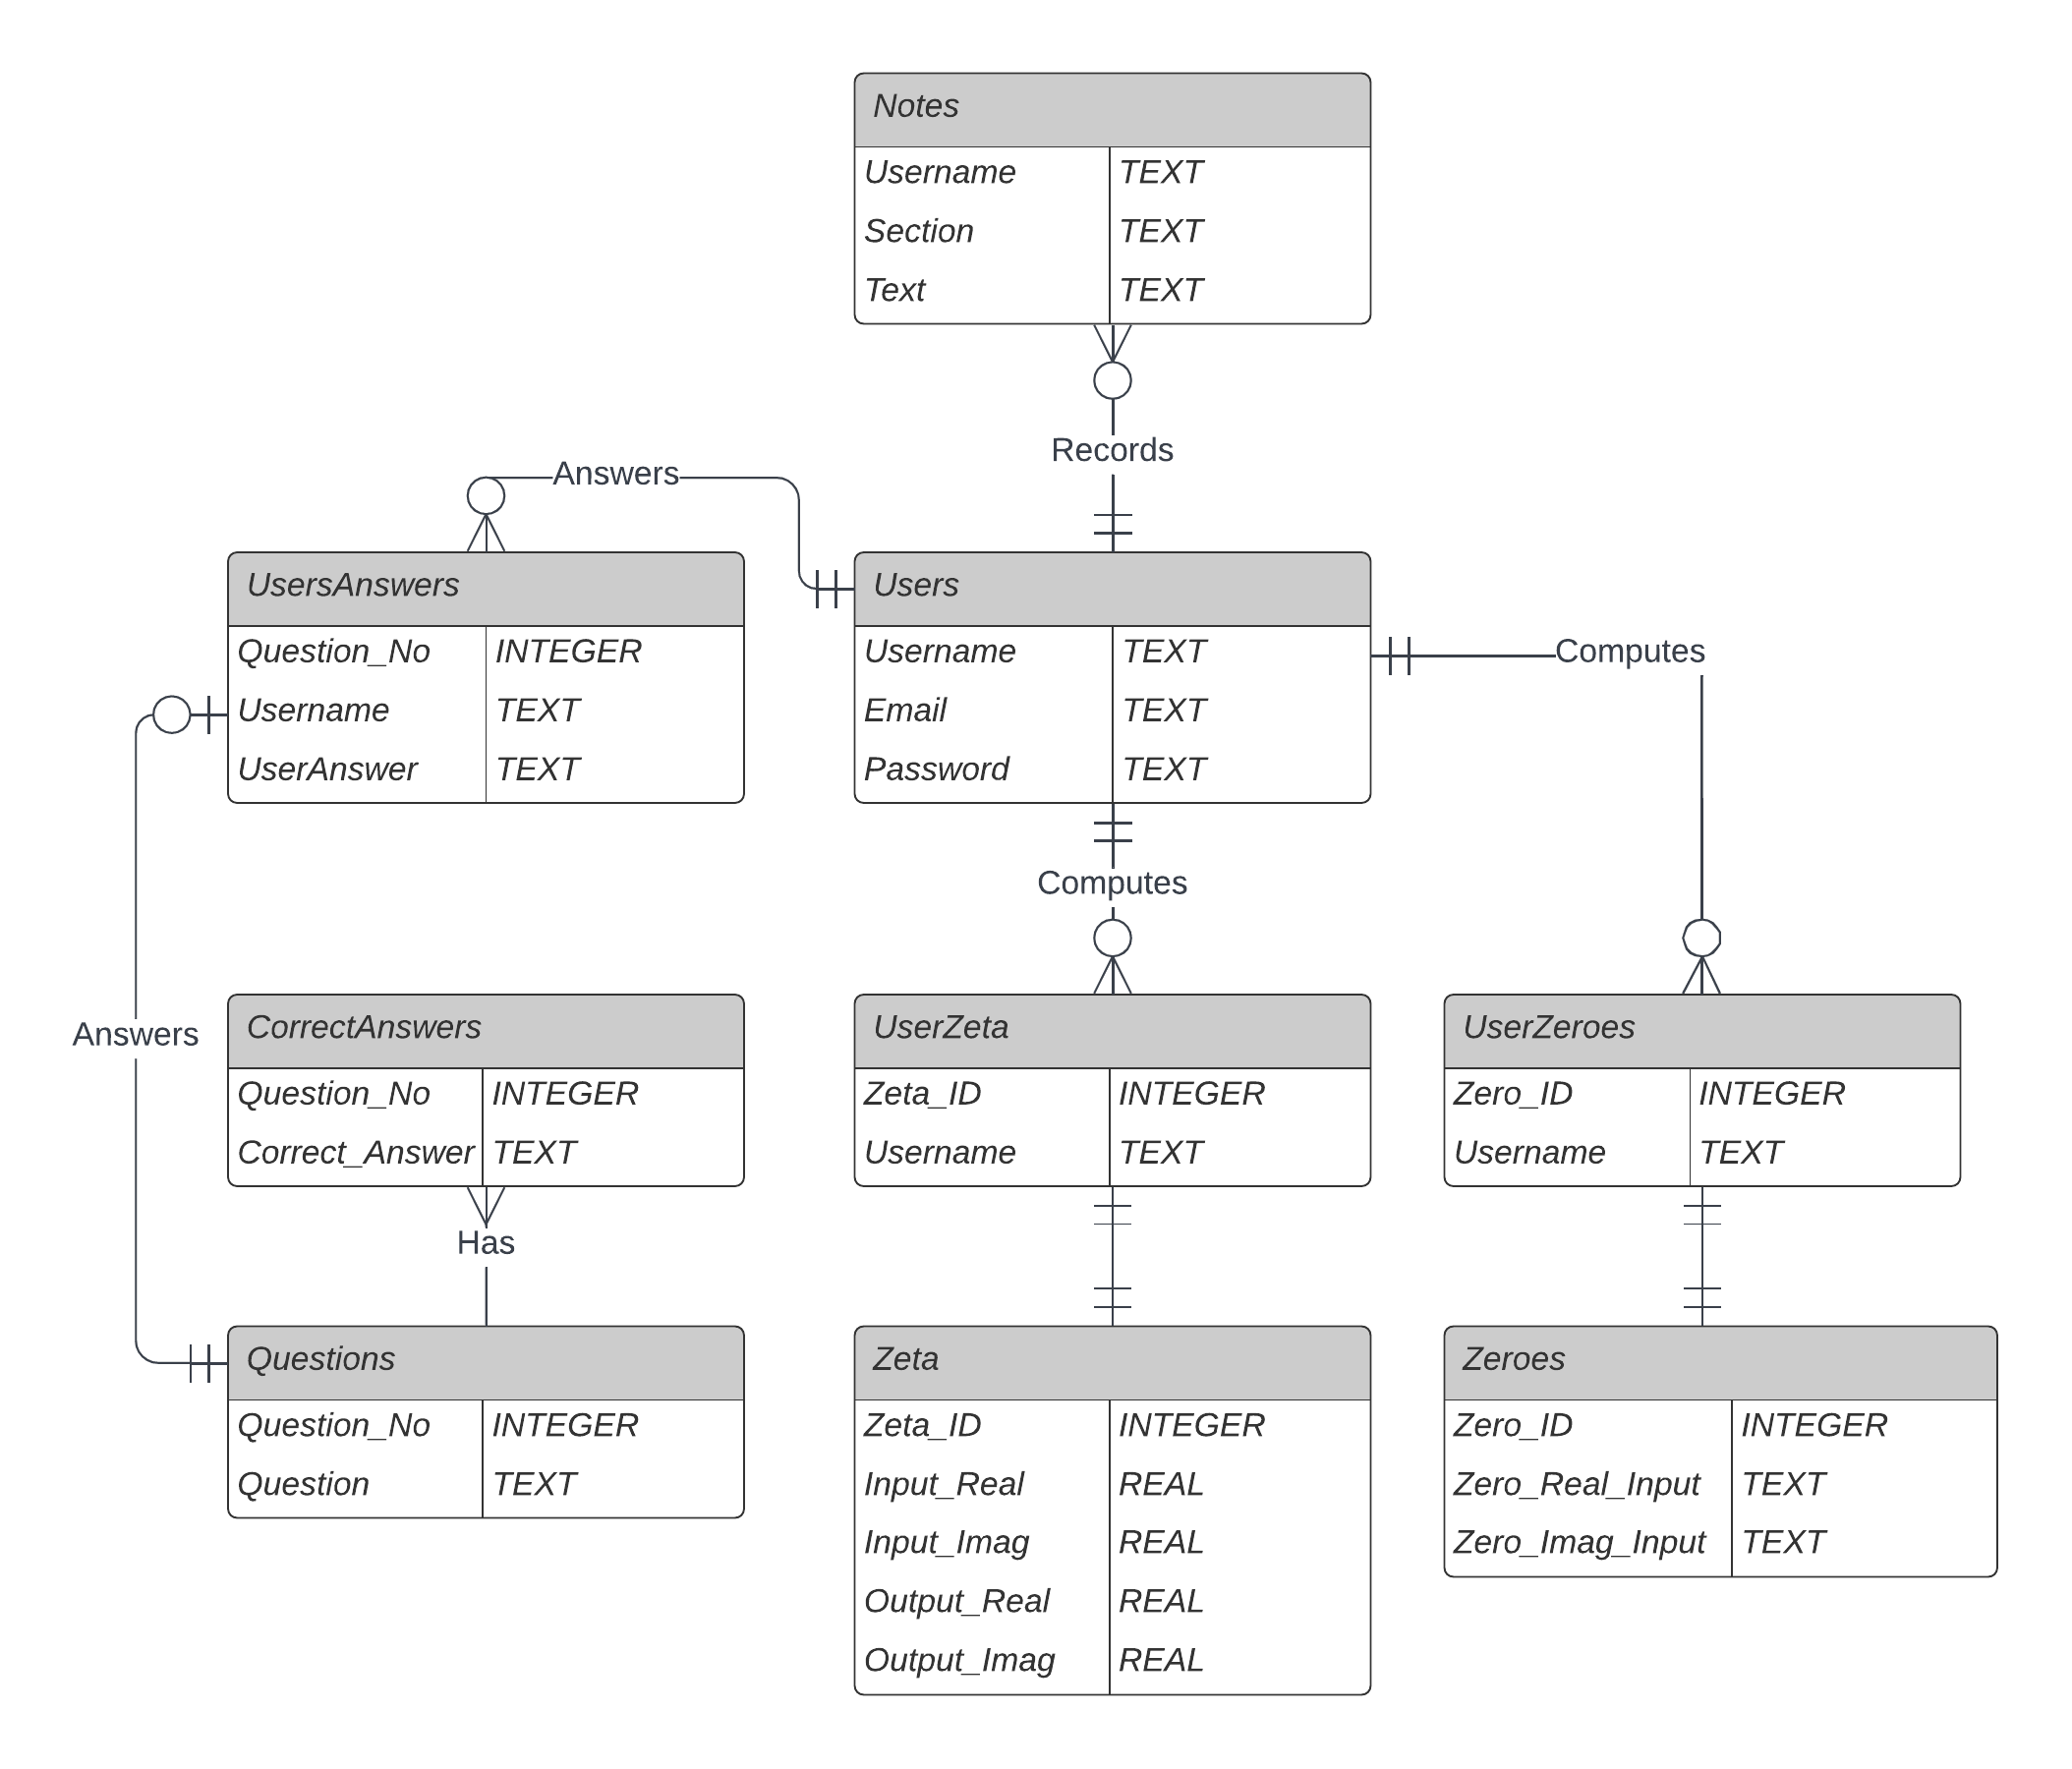
\includegraphics[width=5in]{database-er-diagram}
    \caption{Database Entity Relationship Diagram}
\end{figure}

\textbf{Third Normal Form}

Unlike the previous database that I had designed, this database is now in third normal form. To be in third normal form, a database must meet the following criteria:

First Normal Form:
\begin{itemize}
    \item All rows must be unique
    \item Each cell must contain a single value
    \item Data must be atomic
\end{itemize}
Second Normal Form:
\begin{itemize}
    \item Must be of first normal form
    \item Contains no partial dependencies
\end{itemize}
Third Normal Form:
\begin{itemize}
    \item Must be of second normal form
    \item Contains no non-key dependencies
\end{itemize}
\clearpage
Since redesigning the database, there are now no non-key dependencies, no partial dependencies, all data is atomic, each cell only contains one value and all of the rows are unique, meaning that this database is now in third normal form. This helps throughout the creation of my technical solution, as data will be easier to change and maintain, there will be no duplication of data, meaning that data integrity is maintained, and smaller tables with fewer fields allows for faster searches.

\subsubsection{User Interface Redesign}
Although my screen designs will look the same in the technical solution as they did in my design, I have made vast changes to how these designs will be implemented and displayed throughout the program.

Each page in the GUI will have it's own file in the \textbf{user\_interface} directory. Each of these files will contain a class that is used to configure the correct GUI for that page. Then, in the \textbf{program} directory, there will be a python file for each of the different sections of the program. In each of these python files there will be a class for each page of the GUI. This class creates an instance of the class used to configure the GUI and actually displays the page. Each of these classes then inherits methods and attributes from a class for that overall section, which sets up key buttons and tabs to function properly and contains some methods that are run frequently in the different classes for each page.

These section classes then inherit methods and attributes from a main Screen class, which has some commonly run functions and procedures in it.

There are also separate files and classes that are used to display graphs, as these are displayed in the program as their own screens. There is one class for a graph that is static and one for dynamic graphs.

Below is a class diagram for the tutorial section, showing how all of these classes relate to each other.

\clearpage
\begin{figure}[ht]
    \centering
    \captionsetup{justification=centering}
    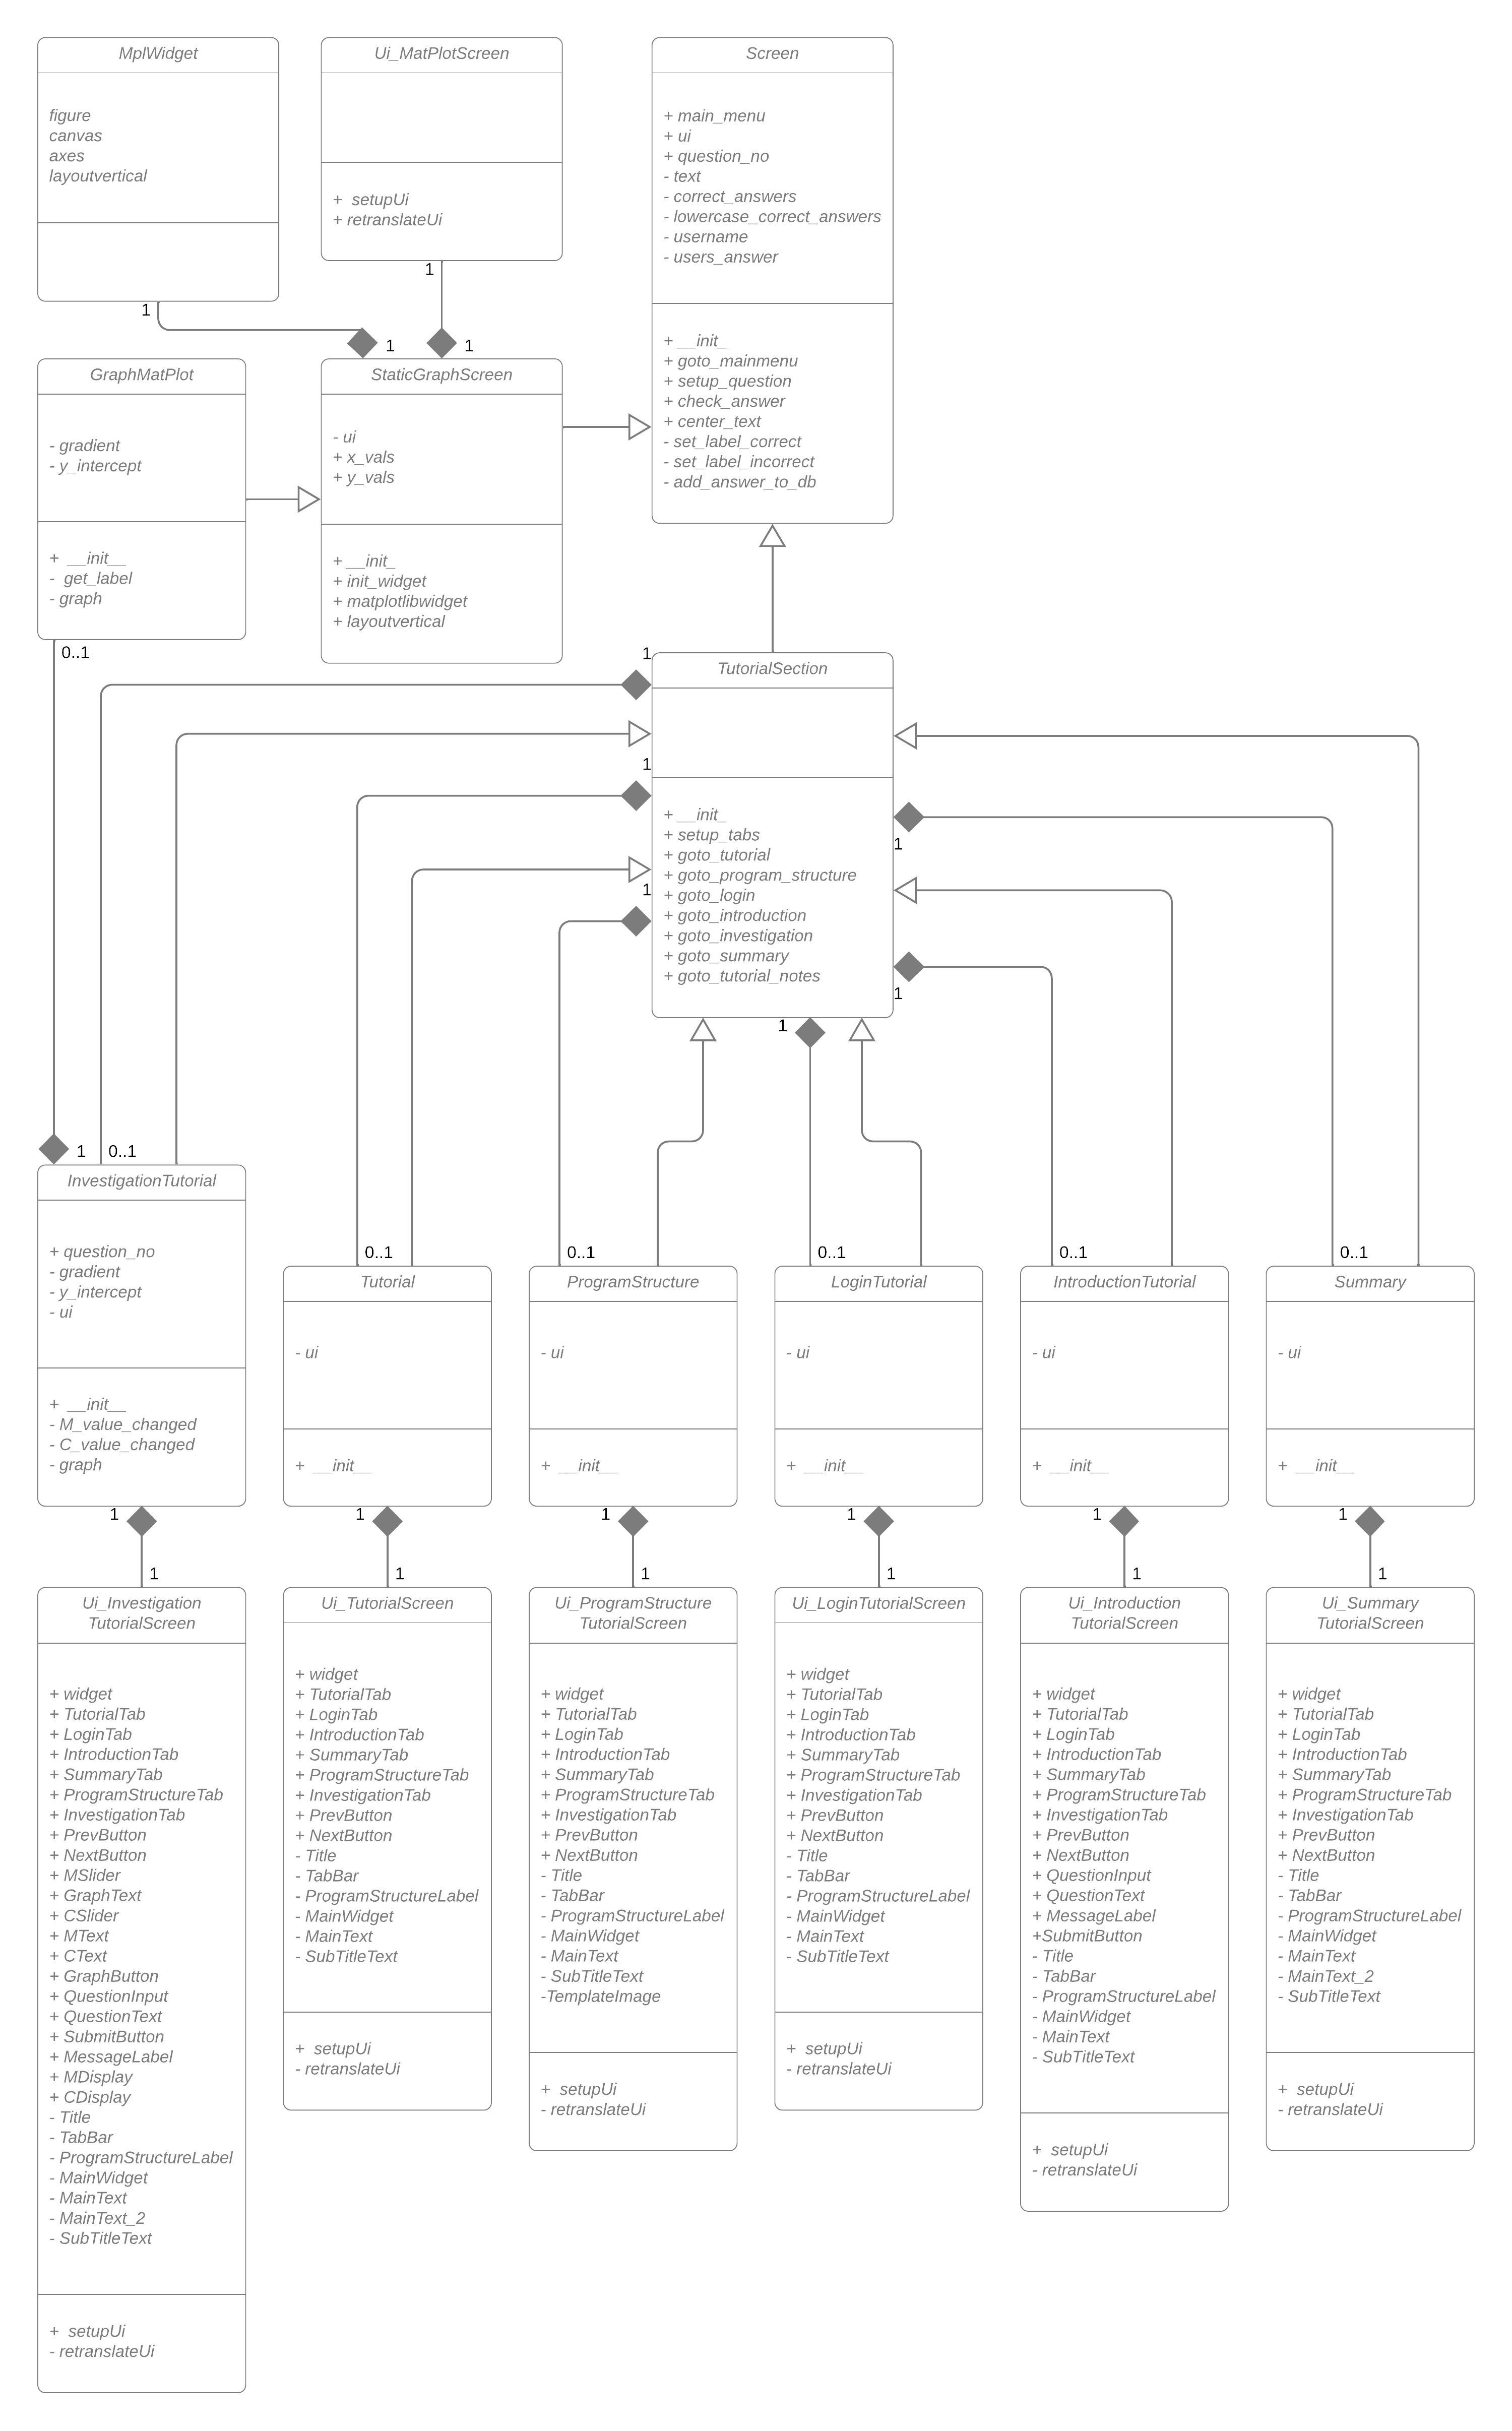
\includegraphics[width=6in]{tutorial-class-diagram}
    \caption{Tutorial Class Diagram}
\end{figure}
\clearpage

If we look at the investigation screen in this tutorial section, we can see that we initially have the Ui\_InvestigationTutorialScreen class; which is used to configure the GUI for this page. This class is then in instance of the InvestigationTutorial class, which displays the Investigation Tutorial Screen and contains methods used for displaying the graph and updating the display when the sliders change.

This InvestigationTutorial class then inherits and is an instance of the TutorialSection class, which contains methods that are used throughout the different classes in the tutorial section.

The TutorialSection class then inherits methods and attributes from the Screen class, which contains methods and functions that are used in screen classes throughout the program.

However, the InvestigationTutorial class also has an instance of the GraphMatPlot class, which is used to set up the graph screen for that page. The GraphMatPlot screen then inherits methods and attributes from the StaticGraphScreen class.

The StaticGraphScreen class has creates instances of the UI\_MatPlotScreen class and the MplWidget class, which together allow a new page to be created with a graph on it. The StaticGraphScreen class also inherits attributes from the Screen class.

This setup may seem overly complex for simply showing a GUI, however, it has been designed such that there is no repeated code, and each class is used for just one purpose.

\clearpage

\subsection{Full Technical Solution}

See \url{https://github.com/jackm245/Riemann-Hypothesis/} for the full write-up, or appendix A at the bottom of this document

\subsection{Code Contents Page}

\begin{table}[ht]
    \centering
    \begin{tabular}{|p{0.26\linewidth}|p{0.59\linewidth}|}
    \hline
    \multicolumn{2}{|c|}{\textbf{Code Contents Page - 1}}\\
    \hline
    \hline
    \textbf{Code} & \textbf{Description}\\
    \hline
    main function & The main entry point to the program\\
    \hline
    MainMenu class & Displays the main menu\\
    \hline
    Progress class & Displays the user's progress through the program\\
    \hline
    LoginSection class & The login system, inherited by all other login classes\\
    \hline
    ResetPassword2 class & Allows the user to permanently change their passwords\\
    \hline
    ResetPassword class & Screen that requires user to login before password change\\
    \hline
    ForgottenPassword2 class & User enters verification code to prove identity\\
    \hline
    ForgottenPassword class & Verification code sent to user's email\\
    \hline
    SignUp class & Allows for the creation of a new user\\
    \hline
    Login class & Allows a user to sign in to an account\\
    \hline
    TutorialSection class & Main class for the tutorial, inherited by all other tutorial classes\\
    \hline
    Tutorial class & Entry point to the tutorial section\\
    \hline
    ProgramStructure class & Displays the Program Structure Tutorial Screen\\
    \hline
    LoginTutorial class & Displays the Login Tutorial Screen\\
    \hline
    IntroductionTutorial class & Displays the Introduction Tutorial Screen\\
    \hline
    InvestigationTutorial class & Displays the Investigation Tutorial Screen\\
    \hline
    GraphMatPlot class & Displays graph in the Investigation Tutorial Screen\\
    \hline
    SummaryTutorial class & Displays the Summary Tutorial Screen\\
    \hline
    IntroductionSection class & Main class for the introduction, inherited by all other introduction classes\\
    \hline
    Introduction class & Entry point to the Introduction section\\
    \hline
    HistoricalBackground class & Displays the Historical Background Screen\\
    \hline
    \end{tabular}
    \caption{Code Contents Page - 1}
\end{table}
\clearpage

\begin{table}[ht]
    \centering
    \begin{tabular}{|p{0.26\linewidth}|p{0.59\linewidth}|}
    \hline
    \multicolumn{2}{|c|}{\textbf{Code Contents Page - 2}}\\
    \hline
    \hline
    \textbf{Code} & \textbf{Description}\\
    \hline
    WhatIsTheRiemann \text{ }  \text{ } Hypothesis class & Displays the What is the Riemann Hypothesis Screen\\
    \hline
    PracticalApplications class & Displays the Practical Applications Screen\\
    \hline
    InvestigationSection class & Main class for the investigation, inherited by all other investigation classes\\
    \hline
    CalculateZeroes2 class & Displays the zeta zeroes that the user has calculated\\
    \hline
    CalculateZeroes class & Asks the user how many zeta zeroes they want to calculate\\
    \hline
    Zeroes class & Displays the zeroes screen in the investigation\\
    \hline
    CalculatorLeaderboard class & Displays the zeroes screen in the investigation\\
    \hline
    TableCalculator2 class & Displays the zeta values that the user calculated\\
    \hline
    TableCalculator class & Allows the user to input values for the table calculator\\
    \hline
    SingleCalculator class & Allows the user to calculate values of the zeta function\\
    \hline
    Calculator class & Displays the calculator screen in the investigation section\\
    \hline
    PrimeNumbers class & Displays the prime numbers screen in the investigation section\\
    \hline
    ZetaApproximation \text{ } \text{ } MatPlot class & Displays a graph showing the convergent  nature of the riemann zeta function\\
    \hline
    ZetaApproximation class & Allows the user to input a value to graph\\
    \hline
    PrimeCountingFunction MatPlot class & Displays a graph of the prime counting function and other related functions\\
    \hline
    PrimeCountingFunction MatPlot class & Displays a graph of the prime counting function and other related functions\\
    \hline
    PrimeCountingFunction class & Displays the prime counting function screen\\
    \hline
    ZetaZeroesMatPlot class & Displays a graph of the zeta zeroes\\
    \hline
    ZetaZeroesPlot class & Displays the zeta zeroes mat plot screen\\
    \hline
    PolarGraphMatPlot class & Displays a polar graph of the zeta function\\
    \hline
    PolarGraph class & Asks the user for an input for the polar graph\\
    \hline
    GraphPlot class & Entry point to the investigation section\\
    \hline
    \end{tabular}
    \caption{Code Contents Page - 2}
\end{table}
\clearpage


\begin{table}[ht]
    \centering
    \begin{tabular}{|p{0.26\linewidth}|p{0.59\linewidth}|}
    \hline
    \multicolumn{2}{|c|}{\textbf{Code Contents Page - 3}}\\
    \hline
    \hline
    \textbf{Code} & \textbf{Description}\\
    \hline
    SummarySection class & Class inherited by all other classes in the summary section\\
    \hline
    Summary class & Main entry point to the summary section\\
    \hline
    TheoryRecap class & Displays the theory recap screen\\
    \hline
    InvestigationResults class & Displays the investigation results screen\\
    \hline
    Conclusion class & Displays the conclusion and \& evaluation screen\\
    \hline
    Imapct class & Displays the impact screen\\
    \hline
    Notes class & A class inherited by all other classes in the notes section\\
    \hline
    TutorialNotes class & Allows the user to make notes on the tutorial\\
    \hline
    IntroductionNotes class & Allows the user to make notes on the introduction\\
    \hline
    InvestigationNotes class & Allows the user to make notes on the investigation\\
    \hline
    SummaryNotes class & Allows the user to make notes on the summary\\
    \hline
    utils directory & Contains key functions, procedures and algorithms that are used throughout the program\\
    \hline
    binary\_search function & Searches for a target in a set of data with time complexity O(log n)\\
    \hline
    binary\_insertion\_sort function & Sorts a set of data efficiently using a queue\\
    \hline
    Queue class & An abstract data structure of a FIFO Queue\\
    \hline
    Stack class & An abstract data structure of a LIFO Stack\\
    \hline
    save\_zeta\_to\_file \phantom{text} function & Uses the binary insertion sort and dictionaries to save data to a csv file\\
    \hline
    change\_datatype \phantom{text} function & Uses structural pattern matching to change the datatype of a variable, when the datatype is given as a string \\
    \hline
    cryptography\_functions file & Contains functions used for hashing password\\
    \hline
    database\_query \phantom{text} function & A function used to easily be able to query the database \\
    \hline
    create\_database \phantom{text} function & Creates the database and all of its tables, populating some of the tables\\
    \hline
    get\_id function & Uses recursion to auto increment the ID for a table in the database\\
    \hline
    email\_functions file & Sends the verification code to the user's email if they have forgotten their password\\
    \hline
    touch function & Uses exception handling to create a file\\
    \hline
    remove function & Uses exception handling to remove a file\\
    \hline
    \end{tabular}
    \caption{Code Contents Page - 3}
\end{table}
\clearpage


\begin{table}[ht]
    \centering
    \begin{tabular}{|p{0.26\linewidth}|p{0.59\linewidth}|}
    \hline
    \multicolumn{2}{|c|}{\textbf{Code Contents Page - 4}}\\
    \hline
    \hline
    \textbf{Code} & \textbf{Description}\\
    \hline
    ncr function & Uses iterables to compute factorials and thus the binomial coefficient\\
    \hline
    zeta function & Uses generators to compute the riemann zeta function for complex numbers\\
    \hline
    sieve\_of\_eratosthenes function & Uses numpy arrays to find all prime numbers up to a given limit\\
    \hline
    integration function & Integrate a given mathematical function between two limit\\
    \hline
    exponential\_integral \text{ } function & Calculates the exponential integral for a given input\\
    \hline
    prime\_power\_function function & Calculates the prime power function\\
    \hline
    Number class & Abstract data type for a given number\\
    \hline
    Complex class & Abstract data type for complex numbers\\
    \hline
    Screen class & Class inherited by all other GUI classes\\
    \hline
    MplWidget class & A GUI widget that allows graphs to be displayed in the GUI\\
    \hline
    StaticGraphScreen class & Default class for displaying static graphs. Creates an instance of MplWidget and inherits Screen class\\
    \hline
    DynamicGraphScreen class & Default class for displaying dynamic graphs. Inherits StaticGraphScreen class\\
    \hline
    ProgramUser class & An instance of this class is used to store the user's credentials during the runtime of the program\\
    \hline
    user\_interface directory & An extensive directory, where each python file is the configuration for the GUI for that page\\
    \hline
    \end{tabular}
    \caption{Code Contents Page - 4}
\end{table}


Although this is not a list of every single class and function in the program, I have included a list of all of the important and complex features. For example, in the utils directory I describe almost every class/functions due to their high significance, whereas with the user\_interface directory, there are 6 folders, 43 files and 40 classes, however all they do is configure the UI which is very repetitive and doesn't require a lot of technical programming skill, thus they have not been mentioned in this contents page.
\clearpage

\subsection{Completeness of Solution}

In this section, I am listing all of the project objectives from my analysis, and whether I have met these objectives. The evidence showing that I have completed these objectives can be seen in my testing video, as well as the source code of the project.

\begin{table}[ht]
    \centering
    \begin{tabular}{|p{0.5\linewidth}|M{0.15\linewidth}|}
    \hline
    \multicolumn{2}{|c|}{\textbf{Completeness of Solution - 1}}\\
    \hline
    \hline
    \textbf{Objective} & \textbf{Achieved}\\
    \hline
    1. The program will be interactive and engaging for the user & Yes\\
    \hline
    1.(a) There will be various questions throughout the program that the user can answer & Yes\\
    \hline
    1.(b) The user will be able to make notes on any of the content in the program & Yes\\
    \hline
    1. (c) The user will be able to choose what they do and where they go in the program, not forced along a single route & Yes\\
    \hline
    1. (d) The user will be able to input their own values into various functions and graphs & Yes\\
    \hline
    2. The user will be able to save their progress through the program via a login system & Yes\\
    \hline
    2. (a) The login system should allow the user to: & Yes\\
    \hline
    2. (a) i. Sign in to their account & Yes\\
    \hline
    2. (a) ii. Create a new account & Yes\\
    \hline
    2. (a) iii. Reset their password if they want to change it & Yes\\
    \hline
    2. (a) iv. Reset their password if they have forgotten it & Yes\\
    \hline
    2. (b) Multiple users will be able to make separate accounts on the system & Yes\\
    \hline
    2. (c) The user’s data such as passwords must be saved securely & Yes\\
    \hline
    2. (d) The user must be able to see how they have progressed throughout the program & Yes\\
    \hline
    \end{tabular}
    \caption{Completeness of Solution Table 1}
\end{table}



\begin{table}[ht]
    \centering
    \begin{tabular}{ | p{0.5\linewidth} | M{0.15\linewidth} |}
    \hline
    \multicolumn{2}{|c|}{\textbf{Completeness of Solution - 2}}\\
    \hline
    \hline
    \textbf{Objective} & \textbf{Achieved}\\
    \hline
    3. The user will be given some background information about the Riemann Hypothesis such that almost anyone could feel comfortable using the program & Yes\\
    \hline
    3. (a) The user should be able to learn the historical background of the Riemann Hypothesis & Yes\\
    \hline
    3. (b) The user should be able to learn what imaginary and complex numbers are & Yes\\
    \hline
    3. (c) The user should be able to learn what the Riemann Hypothesis states & Yes\\
    \hline
    3. (d) The user should be able to learn about the practical applications of the Riemann Hypothesis & Yes\\
    \hline
    4. The program will allow the user to plot various graphs in order to develop their understanding of the Riemann Zeta function and allow them to learn about it & Yes\\
    \hline
    4. (a) A polar graph of the Riemann Zeta Function & Yes\\
    \hline
    4. (b) A graph of the prime counting function, and other related functions used to estimate it & Yes\\
    \hline
    4. (c) A graph of the zeroes of the Riemann Zeta Function & Yes\\
    \hline
    4. (d) A visualisation of the convergence of the infinite series in the Riemann Zeta Function & Yes\\
    \hline
    5. The user will be able to calculate specific values of the Riemann Zeta Function & Yes\\
    \hline
    5. (a) A single calculator, where the user inputs a complex input and receives an output & Yes\\
    \hline
    \end{tabular}
    \caption{Completeness of Solution Table 2}
\end{table}


\begin{table}[ht]
    \centering
    \begin{tabular}{ | p{0.5\linewidth} | M{0.15\linewidth} |}
    \hline
    \multicolumn{2}{|c|}{\textbf{Completeness of Solution - 3}}\\
    \hline
    \hline
    \textbf{Objective} & \textbf{Achieved}\\
    \hline
    5. (b) A table calculator, where the user can calculate the zeta function for a range of input values& Yes\\
    \hline
    5. (c) A leaderboard showing how many values of the zeta function, each user has computed & Yes\\
    \hline
    5. (d) The program will allow the user to store these value(s) to a database and to a csv file & Yes\\
    \hline
    6. The user will be able to calculate the zeroes of the Riemann Zeta Function & Yes\\
    \hline
    6. (a) The user will input how many zeroes they want to calculate & Yes\\
    \hline
    6. (b) The program will calculate these zeroes & Yes\\
    \hline
    6. (c) The zeroes will be displayed to the user in a table & Yes\\
    \hline
    7. The user will be able to store the data that they have collected & Yes\\
    \hline
    7. (a) The program will include a database of multiple values and zeroes of the zeta function & Yes\\
    \hline
    7. (a) i. The user will be able to store values of the zeta function & Yes\\
    \hline
    7. (a) ii. The user will be able to store the non-trivial zeta zeros & Yes\\
    \hline
    7. (a) iii. The user program will retrieve data from the database and display its contents suitably to the user & Yes\\
    \hline
    8. The Program will have a graphical user interface & Yes\\
    \hline
    \end{tabular}
    \caption{Completeness of Solution Table 3}
\end{table}
\clearpage
\section{Testing}
\subsection{Iterative Testing}

\textbf{Imports}

With many different python files with many different functions and classes, imports are imperative to make sure that  every function/class can get accessed from where it needs to. Especially with many directories and subdirectories in the project - the file structure does not make imports easy.

Initially, when writing investigation\_section.py, I needed to import the Complex class from utils/number\_systems.py. So I tried too:

\begin{lstlisting}
from utils/number_systems import Complex
\end{lstlisting}

But this returned an error. So I tried many variations of this such that

\begin{lstlisting}
from utils.number_systems import Complex
\end{lstlisting}

And

\begin{lstlisting}
from utils import number_systems.Complex
\end{lstlisting}

\begin{lstlisting}
from number_systems import Complex
\end{lstlisting}

Until I found out the I need to create a \_\_init\_\_.py file in the utils/ directory. \_\_init\_\_ files are used by python to manage import and create modules from subdirectories.
So in utils/\_\_init\_\_.py I Wrote:

\begin{lstlisting}
from .number_systems import Complex
\end{lstlisting}

This makes utils its own module that can be imported from elsewhere. So now in investigation\_section.py I Wrote:

\begin{lstlisting}
from .utils import Complex
\end{lstlisting}

This then allows me to import the Complex class, although it's inside a different file which is inside a different directory.

But this wasn't the end of it. When now trying to create a button that goes from the investigation\_section to the main\_menu, I tried to write

\begin{lstlisting}
from .main_section import main_menu
\end{lstlisting}

However, as I was also trying to import investigation\_section from main\_section, this gave me a circular import error. So instead of importing the main\_menu when at the top of the file, instead, it has to be imported from within the function it is run.

\begin{lstlisting}
def goto_mainmenu(self):
    from ..main_section import MainMenu
    self.main_menu = MainMenu()
    self.hide()
\end{lstlisting}

Which seems slightly unpythonic, but in practice it is the only way to get around this circular import error, unless I totally redesign the file structure of my code.


\textbf{Zeta Zeroes}

I encountered various different errors when creating the algorithm to find the non-trivial zeta zeroes. The only way I am able to compute the zeta zeroes is through brute force - trying every single possibility before I get them. If this weren't the case, the Riemann Hypothesis would already be solved. When brute forcing to try and get the zeta zeroes, I let the real part of the input to the zeta function be $\frac{1}{2}$, and let the imaginary part of the input be a function of time. Such that as the time spent trying to compute the zeroes increases, the imaginary part of the input increases. The first issue was to do with the accuracy of the input values and output. When changing the imaginary part of the input, if I incremented this value too much, then I could potentially skip over possible zeroes. For example, the first zeta zero is at 14.1, but if I increase the imaginary input by 0.2 every time the graph updates, then I would calculate $\zeta(14.0)$ and $\zeta(14.2)$, but completely skip 14.1, meaning that I would have missed a zero. However, if I increment the imaginary input by too small of a number, then the program will take longer to find each zero, and it could accidentally double count some zeroes. If the imaginary input incremented by $0.001$ each time, then it might mistake 14.099, 14.100, and 14.101 as three zeroes, even though there was only one there.

On order to solve this problem, I used the method of trial and improvement until I got an algorithm that was fast, and didn't overcount or undercount.Eventually, I came up with the algorithm that

\begin{lstlisting}
def is_zeta_zero(real, imag):

    """
    Given a complex number, the function checks to see if this number is
    approximately a root (zero) of the Riemann Zeta Function
    """

    zeta_value = zeta(real, imag)
    return abs(zeta_value) < 10e-3

def find_zeta_zeroes(no_of_zeroes):
    zeroes = Queue()
    count = 0
    while zeroes.get_size() < no_of_zeroes:
        accuracy = count // 500 + 100
        real = 1/2
        imag = count / accuracy
        if is_zeta_zero(real, imag) and [real, round(imag, 1)] not in zeroes.get_queue():
            zeroes.enQueue([real, round(imag, 1)])
        count += 1
    return zeroes
\end{lstlisting}

Where count is a function of time and updates at regular intervals, such that changing the imag input by $\frac{count}{accuracy}$, when accuracy = $\frac{count}{500} + 100$, allows zeta zeroes to be calculated by a high precision while also not trying so many values that the algorithm takes ages. Furthermore, having the range of values from -0.001 to 0.001 for the zero to be in further ensures that no zeroes get skipped. However, the drawback of this is that it does take a long time, and I am also only able to measure the zeroes to 1 decimal place, or I get too many repeats.

To test that these changes worked, I used the Calculate Zeroes screen. This test table shows the accuracy of the function after going through various stages of trial and improvement.

\begin{table}[ht]
    \centering
\begin{tabular}{| M{0.08\linewidth} | p{0.14\linewidth} | p{0.12\linewidth} | p{0.12\linewidth} | p{0.11\linewidth} |p{0.18\linewidth}|}
    \hline
    \multicolumn{6}{|c|}{\textbf{Zeta Zeroes Test Table}}\\
    \hline
    \hline
    \textbf{Test \#} & \textbf{Input} & \textbf{Expected Output} & \textbf{Actual Output} & \textbf{Outcome} & \textbf{Comments}\\
    \hline
    1 & 1  & 14.1 & & Pass & \\
    \hline
    2 & 2  & 14.1, 21.0& & Pass & \\
    \hline
    3 & 5  & 14.1, 21.0, 25.0, 30.4, 30.4 & 14.1, 21.0, 25.0, 30.4, 32.9 & Pass & Double counts one zero\\
    \hline
    4 & 7  & 14.1, 21.0, 25.0, 30.4, 30.4, 32.9, 37.6 & 14.1, 21.0, 25.0, 30.4, 32.9, 37.6, 40.9 & Pass & \\
    \hline
    \end{tabular}
    \caption{Zeta Zeroes Test Table}
\end{table}

As can be seen from the test table, this is not a perfect calculator of the zeta zeroes. Although on test cases 3 and 4, the expected output was not exactly equal to the actual output, this can be excused for various reasons. There is no way to exactly calculate the zeta zeroes, and with a not very powerful machine, it would take far too long to be able to accurately compute every zero to a high degree of accuracy. So in order to still be able to calculate the zeroes in good time, there is a trade off with having some double counts or miss counts of zeroes. Furthermore, in order to keep the time that this takes to run to a small enough amount, I am only able to calculate the zeta zeroes to 1 decimal place.

Overall, the function that I have written works well to get a rough idea of the zeta zeroes, but to calculate them accurately, it would take far longer than is reasonable for this program and would require some very large computers to do so.

\begin{figure}[h]
    \centering
    \captionsetup{justification=centering}
    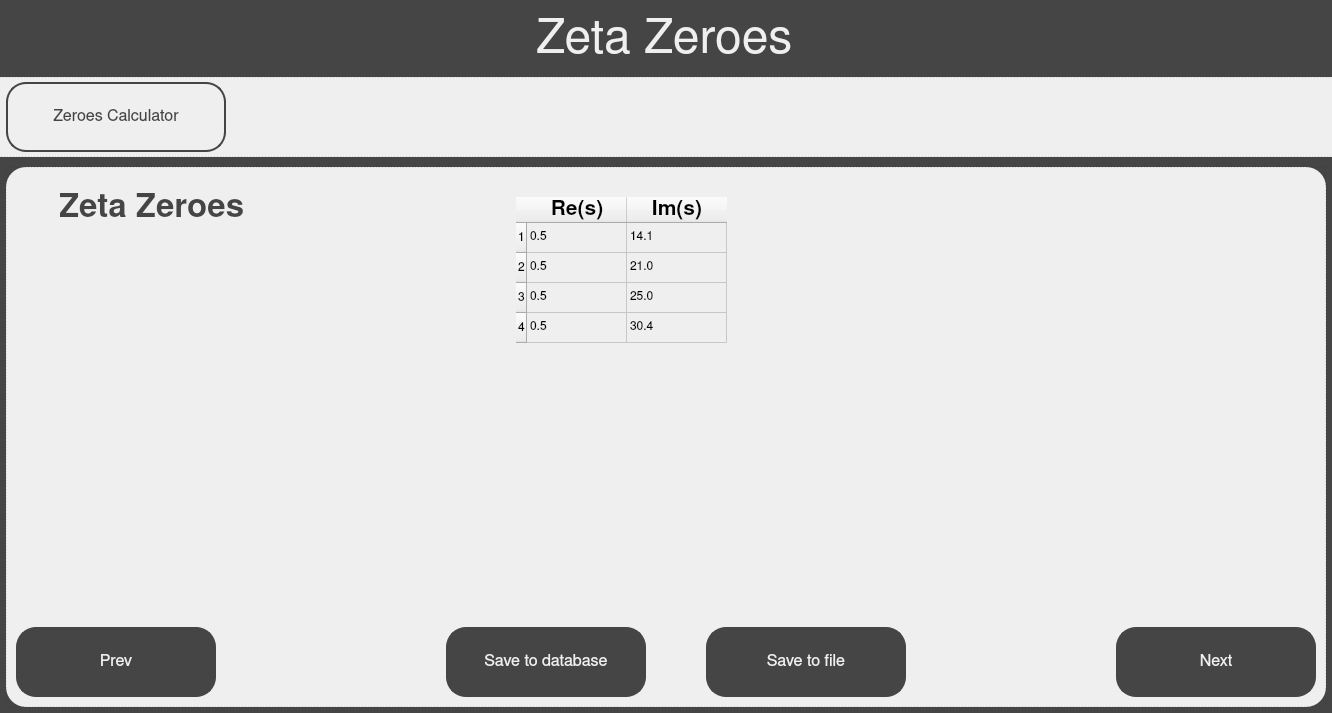
\includegraphics[width=4in]{zero-table-ev}
    \caption{Evidence of the Zeta Zeroes Table}
\end{figure}
\clearpage



\subsection{Post-Development Testing}

This post-development testing was done in my testing video, so see my testing video for evidence of this.

\begin{table}[ht]
    \centering
    \begin{tabular}{|p{0.06\linewidth} | M{0.08\linewidth} | p{0.14\linewidth} | p{0.12\linewidth} | p{0.12\linewidth} | p{0.11\linewidth} |p{0.18\linewidth}|}
    \hline
    \multicolumn{7}{|c|}{\textbf{Post-Development Test Table - 1}}\\
    \hline
    \hline
    \textbf{Obje ctive} & \textbf{Test \#} & \textbf{Input} & \textbf{Expected Output} & \textbf{Actual Output} & \textbf{Outcome} & \textbf{Comments}\\
    \hline
    1. & & & & & & All parts of objective completed and passed \\
    \hline
    1.(a) & 1 & 14.1  & Correct! & Correct! & Pass & \\
    \hline
     & 2 & 14.1  & Correct! & Correct! & Pass & \\
    \hline
     & 3 & i  & Correct! & Correct! & Pass & \\
    \hline
     & 4 & k  & Incorrect, try again & Incorrect, try again & Pass & \\
    \hline
     & 5 & j  & Correct! & Correct! & Pass  & \\
    \hline
    1.(b) & 6 & Attempt to change text & Text does not change & Text does not change & Pass & \\
    \hline
    & 7 & Tutorial & Tutorial & Tutorial & Pass & \\
    \hline
    & 8 & Save button clicked & Note Saves & Note Saves & Pass & \\
    \hline
    & 9 & Notes button clicked from Introduction & Go to Introduction Notes & Go to Introduction Notes & Pass & \\
    \hline
    & 10 & Notes button clicked from Summary & Go to Summary Notes & Go to Summary Notes & Pass & \\
    \hline
    1.(c) & 11 & Click on tabs & Screen changes to the corresponding page & Screen changes to the corresponding page & Pass & \\
    \hline
    1.(d) & 12 & 9 & Polar Graph $\zeta(9)$ & Polar Graph $\zeta(9)$ & Pass & \\
    \hline
    \end{tabular}
    \caption{Post Development Test Table - 1}
\end{table}
\clearpage
\begin{table}[ht]
    \centering
    \begin{tabular}{|p{0.06\linewidth} | M{0.08\linewidth} | p{0.14\linewidth} | p{0.12\linewidth} | p{0.12\linewidth} | p{0.11\linewidth} |p{0.18\linewidth}|}
    \hline
    \multicolumn{7}{|c|}{\textbf{Post-Development Test Table - 2}}\\
    \hline
    \hline
    \textbf{Obje ctive} & \textbf{Test \#} & \textbf{Input} & \textbf{Expected Output} & \textbf{Actual Output} & \textbf{Outcome} & \textbf{Comments}\\
    \hline
    & 13 & 0 & Polar Graph $\zeta(0)$ & Polar Graph$\zeta(0)$ & Pass & \\
    \hline
    & 14 & 1+1i & 0.582-0.927i & 0.582-0.927i & Pass & \\
    \hline
    & 15 & 3+2i & 0.973-0.148i & 0.973-0.148i & Pass & \\
    \hline
    2. & & & & & & All parts of objective completed and passed \\
    \hline
    2. (a) & & & & & & Showcased in video and as a collection of objectives \\
    \hline
    2.(a)i. & 16 & & Username or password is not valid & Username or password is not valid & Pass & \\
    \hline
    & 17 & asdasdasd, asdasdasd & Username or password is not valid & Username or password is not valid & Pass & \\
    \hline
    & 18 & TestUser1, Password1 & Go to main menu & Go to main menu & Pass & \\
    \hline
    2.(a)ii. & 19 & submit button clicked & Email address must be valid & Email address must be valid & Pass & \\
    \hline
    & 20 & test3@ domain .com & Password must contain... & Password must contain... & Pass & \\
    \hline
    & 21 & Password3, Password4 & Passwords do not match & Passwords do not match & Pass & \\
    \hline
    & 21 & Password3, Password3 & Go to main menu & Go to main menu & Pass & \\
    \hline
    2.(a)iii. & 22 & kegeno 4324@procowork .com & Go to forgotten password 2 page & Go to forgotten password 2 page & Pass & \\
    \hline
    & 23 & 602750 & Go to reset password 2 page & Go to reset password 2 page & Pass & \\
    \hline
    & 24 & TestPassword1, TestPassword & Passwords do not match & Passwords do not match & Pass & \\
    \hline
    \end{tabular}
    \caption{Post Development Test Table - 2}
\end{table}
\clearpage
\begin{table}[ht]
    \centering
    \begin{tabular}{|p{0.06\linewidth} | M{0.08\linewidth} | p{0.14\linewidth} | p{0.12\linewidth} | p{0.12\linewidth} | p{0.11\linewidth} |p{0.18\linewidth}|}
    \hline
    \multicolumn{7}{|c|}{\textbf{Post-Development Test Table - 3}}\\
    \hline
    \hline
    \textbf{Obje ctive} & \textbf{Test \#} & \textbf{Input} & \textbf{Expected Output} & \textbf{Actual Output} & \textbf{Outcome} & \textbf{Comments}\\
    \hline
    & 25 & asdasd, asdasd & Password must contain... & Password must contain... & Pass & \\
    \hline
    & 26 & TestPass word1, TestPassword1 & Go to main menu & Go to main menu & Pass & \\
    \hline
    2.(a)iv. & 27 & TestUser1, TestPassword1 & Go to reset password 2 & Go to reset password 2 & Pass &\\
    \hline
     & 28 & Password1, Password1 & Go to main menu & Go to main menu & Pass & \\
    \hline
    2.(b) & 29 & TestUser2, Password2 & Go to main menu & Go to main menu & Pass & \\
    \hline
    & 30 & TestUser3, Password3 & Go to main menu & Go to main menu & Pass & \\
    \hline
    & 31 & TestUser3's Tutorial Notes, Save & Saved! & Saved! & Pass & \\
    \hline
    2.(c) & 32 & & & & & Video \\
    \hline
    2.(c) & 33 & odd numbers & False & False & Pass & \\
    \hline
    3. & & & & & & All parts of objective completed and passed \\
    \hline
    3.(a) & 34 & Click on Historical Background tab & Go to historical background tab & Go to historical Background tab & Pass & \\
    \hline
    3.(b) & 35 & Click on What is the RH tab & Go What is the RH tab & Go to what is the RH tab & Pass & \\
    \hline
    3.(c) & 35 & Click on What is the RH tab & Go What is the RH tab & Go to what is the RH tab & Pass & \\
    \hline
    3.(d) & 36 & Click on Practical Applications & Go to practical applications & Go to practical applications & Pass & \\
    \hline
    \end{tabular}
    \caption{Post Development Test Table - 3}
\end{table}
\clearpage
\begin{table}[ht]
    \centering
    \begin{tabular}{|p{0.06\linewidth} | M{0.08\linewidth} | p{0.14\linewidth} | p{0.12\linewidth} | p{0.12\linewidth} | p{0.11\linewidth} |p{0.18\linewidth}|}
    \hline
    \multicolumn{7}{|c|}{\textbf{Post-Development Test Table - 4}}\\
    \hline
    \hline
    \textbf{Obje ctive} & \textbf{Test \#} & \textbf{Input} & \textbf{Expected Output} & \textbf{Actual Output} & \textbf{Outcome} & \textbf{Comments}\\
    \hline
    4. & & & & & & All parts of objective completed and passed \\
    \hline
    4.(a) & 37 & abc & Error: Input must be whole number or decimal & Error: Input must be whole number or decimal & Pass & \\
    \hline
    & 38 & 46 & Error: Input value must be between -10 and 45 & Error: Input value must be between -10 and 45 & Pass & \\
    \hline
    & 39 & 45 & Polar Graph & Polar Graph & Pass & \\
    \hline
    & 40 & 44 & Polar Graph & Polar Graph & Pass & \\
    \hline
    & 41 & -9 & Polar Graph & Polar Graph & Pass & \\
    \hline
    & 42 & -10 & Polar Graph & Polar Graph & Pass & \\
    \hline
    & 43 & -11 & Error: Input value must be between -10 and 45 & Error: Input value must be between -10 and 45 & Pass & \\
    \hline
    & 44 & 0.5 & Polar Graph & Polar Graph & Pass & \\
    \hline
    4.(b) & 45 & Graph Button Clicked & Prime Functions Graph & Prime Functions Graph & Pass & \\
    \hline
    4.(c) & 46 & Graph Button Clicked & Zeta Zeroes Graph & Zeta Zeroes Graph & Pass & \\
    \hline
    4.(d) & 47 & abc & Input must be a complex number of the form a+bi & Input must be a complex number of the form a+bi & Pass & \\
    \hline
    \end{tabular}
    \caption{Post Development Test Table - 4}
\end{table}
\clearpage
\begin{table}[ht]
    \centering
    \begin{tabular}{|p{0.06\linewidth} | M{0.08\linewidth} | p{0.14\linewidth} | p{0.12\linewidth} | p{0.12\linewidth} | p{0.11\linewidth} |p{0.18\linewidth}|}
    \hline
    \multicolumn{7}{|c|}{\textbf{Post-Development Test Table - 5}}\\
    \hline
    \hline
    \textbf{Obje ctive} & \textbf{Test \#} & \textbf{Input} & \textbf{Expected Output} & \textbf{Actual Output} & \textbf{Outcome} & \textbf{Comments}\\
    \hline
    4.(d) & 48 & 30-31i & Input is too large, real and imag parts must be between -30 and 30 & & Pass & \\
    \hline
    & 49 & 30-30i & Zeta Approximation Graph & Zeta Approximation Graph & Pass & \\
    \hline
    & 50 & -30-30i & Zeta Approximation Graph & Zeta Approximation Graph & Pass & \\
    \hline
    & 51 & 1 & Input cannot be equal to 1 & Input cannot be equal to 1 & Pass & \\
    \hline
    & 52 & 0+5i & Zeta Approximation Graph & Zeta Approximation Graph & Pass & \\
    \hline
    & 53 & 0-5i & Zeta Approximation Graph & Zeta Approximation Graph & Pass & \\
    \hline
    & 54 & 5-5i & Zeta Approximation Graph & Zeta Approximation Graph & Pass & \\
    \hline
    & 55 & 5+5i & Zeta Approximation Graph & Zeta Approximation Graph & Pass & \\
    \hline
    \end{tabular}
    \caption{Post Development Test Table - 5}
\end{table}
\clearpage
\begin{table}[ht]
    \centering
    \begin{tabular}{|p{0.06\linewidth} | M{0.08\linewidth} | p{0.14\linewidth} | p{0.12\linewidth} | p{0.12\linewidth} | p{0.11\linewidth} |p{0.18\linewidth}|}
    \hline
    \multicolumn{7}{|c|}{\textbf{Post-Development Test Table - 6}}\\
    \hline
    \hline
    \textbf{Obje ctive} & \textbf{Test \#} & \textbf{Input} & \textbf{Expected Output} & \textbf{Actual Output} & \textbf{Outcome} & \textbf{Comments}\\
    \hline
    5. & & & & & & All parts of objective completed\\
    \hline
    5.(a) & 56 & abc  & Input must be a complex number of the form a+bi & Input must be a complex number of the form a+bi & Pass & \\
    \hline
    & 57 & 30+30i  & 1.0-8.67e-10i & 1.0-8.67e-10i & Pass & \\
    \hline
    & 58 & 10000000 + 10000000i  & Real or imag part of input must be less than 50 & Real or imag part of input must be less than 50 & Pass & \\
    \hline
    & 59 & 50+50i & 1.0+8.85e-17i & 1.0+8.85e-17i & Pass & \\
    \hline
    & 60 & 51+51i & Real or imag part of input must be less than 50 & Real or imag part of input must be less than 50 & Pass & \\
    \hline
    & 61 & -50-50i & -9.64e+58 +4.57e+57i & -9.64e+58 +4.57e+57 & Pass & \\
    \hline
    & 62 & -51-51i & Real or imag part of input must be less than 50 & Real or imag part of input must be less than 50 & Pass & \\
    \hline
    & 62 & 1+1i & 0.582-0.927i & -0.582-0.927i & Pass & \\
    \hline
    5.(b) & 63 & 10000+ 1000000i, 100000+ 1000000i, 5 & Calculator Table & Calculator Table & Pass & \\
    \hline
    \end{tabular}
    \caption{Post Development Test Table - 6}
\end{table}
\clearpage

\begin{table}[ht]
    \centering
    \begin{tabular}{|p{0.06\linewidth} | M{0.08\linewidth} | p{0.14\linewidth} | p{0.12\linewidth} | p{0.12\linewidth} | p{0.11\linewidth} |p{0.18\linewidth}|}
    \hline
    \multicolumn{7}{|c|}{\textbf{Post-Development Test Table - 7}}\\
    \hline
    \hline
    \textbf{Obje ctive} & \textbf{Test \#} & \textbf{Input} & \textbf{Expected Output} & \textbf{Actual Output} & \textbf{Outcome} & \textbf{Comments}\\
    \hline
    & 64 & 1+1i, 1+1i, 100000000 & Error & Error & Pass & \\
    \hline
    5.(c) & 65 & Clicked on leaderboard tab & Go to leaderboard screen & Go to leaderboard screen & Pass & \\
    \hline
    5.(d) & 66 & Clicked on Save to database & Values saved to database & Values saved to database & Pass& \\
    \hline
    & 67 & Clicked on save to file & Values saved to file & Values not saved to file & Fail & \\
    \hline
    6. & & & & & & All parts of objective completed and passed\\
    \hline
    6.(a) & 68 & 0 & Error & Error & Pass & \\
    \hline
    & 69 & 0 & Error & Error & Pass & \\
    \hline
    & 70 & 3 & Zeroes Table & Zeroes Table & Pass & \\
    \hline
    6.(b) & & & & & & Video \\
    \hline
    6.(c) & & & & & & Video \\
    \hline
    7. & & & & & & All parts of objective completed and passed\\
    \hline
    7.(a) & & & & & & \\
    \hline
    7.(a)i. & 71 & Save to database clicked & Values saved to database & Values saved to database & Pass & \\
    \hline
    7.(a)ii. & 72 & Save to database clicked & Values saved to database & Values saved to database & Pass & \\
    \hline
    7.(a)iii. & 73 & Progress button clicked & Progress screen displayed & Progress screen displayed & Pass & \\
    \hline
    8. & & & & & & Showcased in the video \\
    \hline
    \end{tabular}
    \caption{Post Development Test Table - 7}
\end{table}

\clearpage

One error which I discovered during my testing was to do with saving values of the zeta function to the csv file. After going back and looking at the problem, I realised that I had a logic error where the csv file was unable to have two records where the InputReal record was the same. This is due to how I chose to sort of the data. The code at the time look as such:

\begin{lstlisting}
def save_zeta_to_file(csv_values, filepath, regex, index, fieldnames):

    """
    Given a list of complex numbers, combine these with the contents of the
    file that they are going to be saved to, sort these values using the first
    real number, and save them back into the csv file
    """

    if not os.path.isfile(filepath):
        os.mknod(filepath)
    with open(filepath, 'r') as csv_file:
        csv_reader = csv.reader(csv_file)
        for row in csv_reader:
            if row != fieldnames:
                csv_values.append(list(map(str, row)))
    sorting_dict = {list(map(float,
        re.findall(regex, ','.join(row))))[index] : row for row in csv_values}
    sorted_keys = binary_insertion_sort(list(set(sorting_dict.keys())))
    sorted_values = [sorting_dict[key] for key in sorted_keys]
    with open(filepath, 'w') as csv_file:
        csv_writer = csv.writer(csv_file)
        csv_writer.writerow(fieldnames)
        for row in sorted_values:
            csv_writer.writerow(row)
\end{lstlisting}

The problems came with lines 16 and 17, which say that

\begin{lstlisting}
    sorting_dict = {list(map(float,
        re.findall(regex, ','.join(row))))[index] : row for row in csv_values}
\end{lstlisting}

This creates a dictionary with the InputReal of each record as the key, and each record as the value, for all of the records in the file. However, if two records had the same InputReal, then they would create the same key. So then when I call

\begin{lstlisting}
    sorted_keys = binary_insertion_sort(list(set(sorting_dict.keys())))
\end{lstlisting}

I am sorting the set of all of the keys. This removes duplicates. However, I have to sort the data as a set, otherwise the binary\_insertion\_sort will not work. So I need to change the data in order to eliminate any two records having the same first value. To do this, I added the number of the record onto the end of each key. This allows each record to still be sorted, and also make them unique.

With these changes, the working function now looks as follows:

\begin{lstlisting}
def save_zeta_to_file(csv_values, filepath, regex, index, fieldnames):

    """
    Given a list of complex numbers, combine these with the contents of the
    file that they are going to be saved to, sort these values using the first
    real number, and save them back into the csv file
    """

    if not os.path.isfile(filepath):
        os.mknod(filepath)
    with open(filepath, 'r') as csv_file:
        csv_reader = csv.reader(csv_file)
        for row in csv_reader:
            if row != fieldnames:
                csv_values.append(list(map(str, row)))
    sorting_dict = {float(str(list(map(float,
        re.findall(regex, ','.join(row))))[index]) + str(row_no)) : row for row_no, row in enumerate(csv_values)}
    sorted_keys = binary_insertion_sort(list(set(sorting_dict.keys())))
    sorted_values = [sorting_dict[key] for key in sorted_keys]
    with open(filepath, 'w') as csv_file:
        csv_writer = csv.writer(csv_file)
        csv_writer.writerow(fieldnames)
        for row in sorted_values:
            csv_writer.writerow(row)
\end{lstlisting}


As evidence that this function now works as expected, here is a screenshot showing the sorted data in the zeta-values.csv file.

\begin{figure}[h]
    \centering
    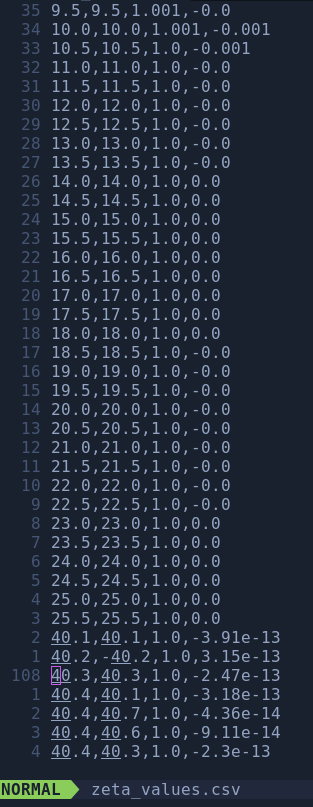
\includegraphics[width=1.5in]{zeta-values-ev}
    \caption{zeta-values.csv file}
\end{figure}

\clearpage

\section{Evaluation}


\subsection{Objective Completion}

In this section, I will list many of the key objectives of my program, and evaluate how well I have achieved them.

\textbf{1. The program will be interactive and engaging for the user}

User input in the forms of questions, notes and inputs to functions are abundant throughout the program. I met this first objective well by adding features that allow the user to actually control what happens in a program, instead of just getting a user to click a 'next' button over and over. Steps have been taken to make this program interactive and I believe that these features make the program both interactive and engaging. This objective has been completed well.

\textbf{1. (a) There will be various questions throughout the program that the user can answer}

In total, there are 10 questions asked to the user. The user's answer is then marked correct or incorrect. And if the user is signed in, their progress is saved, such that their answer is saved and they can see which questions they have answered correctly or incorrectly. I have met this objective.


\textbf{1. (b) The user will be able to make notes on any of the content in the program}

Throughout the program, there are many buttons that the user can click on to access the notes section, so it has been made very accessible. The notes have been split into a separate page for each section, and the user can make their notes as long as they like. This objective has been completed sufficiently.


\textbf{1. (c) The user will be able to choose what they do and where they go in the program, not forced along a single route}

Although there is a sort of default linear way to go through the program using the prev and next buttons, the tab bar on each page allows the user to jump between sections and pages as they wish. Although the actual layout and organisation of the pages could have been made more straightforwards, the user is still able to access all parts of the program at any point, so I have achieved this objective.

\textbf{2. (a) The login system should allow the user to i. Sign in to their account ii. Create a new account iii. Reset their password if they want to change it iv. Reset their password if they have forgotten it}

I am very happy with how they login system turned out in my project. It is very straightforward for the user to login, create an account, or change their password. Two key elements of this that stand out to me are the input validation for the usernames, emails, and passwords - making sure that they are always of the correct type and structure; and also with the emailing of the user when they have forgotten their password - this is very neat. An improvement I could make to the login system would be to add a page or button to log out of an account. This would not be hard to implement at all (just requires updating the User instance of the ProgramUser class), as this would stop the user having to close and reopen the program every time they want to log out of their account. Overall however, the login system does meet all of the objectives and does so well.

\textbf{2. (d) The user must be able to see how they have progressed throughout the program}

The progress section in the program sufficiently completes this objective. It displays to the user which of the questions they have answered, and if they have done so successfully. This allows the user to see what they have gotten right or wrong, and also how much they actually know about the Riemann Hypothesis. If a user starts using this program knowing nothing about the Riemann Hypothesis, then reads through the introduction and uses the investigation, and is then able to answer some, if not all, of the questions, then they have made significant progress, not just through the program but of their understanding of the Riemann Hypothesis, and this is shown on the progress page. Therefore, I have achieved this objective.

\textbf{3. The user will be given some background information about the Riemann Hypothesis such that almost anyone could feel comfortable using the program}

Through the tutorial and the introduction section, the user is given sufficient explanations regarding to the historical background of the Riemann Hypothesis, what complex numbers are, what the Riemann Hypothesis is, and what the practical applications of the hypothesis are. This information is then solidified as knowledge through the questions asked in the program, showing that the user has understood what they've read and learnt. Through these pages in the introduction section, I have reached objectives 3. (a), 3. (b), 3. (c) and 3, (d), thus meeting the overall objective 3 sufficiently. However, it would help the user understand a lot more about the program if they had a more in-depth knowledge than the information that is said during the introduction. The problem is that this project is not solely about teaching people what the hypothesis is, and reading pages and pages of information about the hypothesis would more than likely not be interesting to the user - they could just go to the wikipedia page for that. Overall, I think this program has a good balance of introductory knowledge teaching while also allowing the user to actually investigate the Hypothesis.


\textbf{4. (a) A polar graph of the Riemann Hypothesis}

Overall, most of the graphs I created in the project were clear in what they showed, and allowed the user to understand further what the Riemann Hypothesis is about. However, I am especially pleased with the turn out of this graph. Going from iteration to iteration of the zeta function, eventually finding a way of computing it such that the graph appears to calculate values of the zeta function took a lot of research but definitely was worth the while. An improvement that could be made to not just this graph but also other ones is to make them more interactive for the user. This would entail, for example, the user being able to hover with the mouse over different parts of the graph, and be shown a pop-up of the input and output of that point, or having the graph change colour slightly as the imaginary input increases with time. It's small additions like this that would make the program more appealing to use and provide just that much more useful information.

\textbf{4. (d) A graph of the zeroes of the Riemann Zeta Function}

The zeroes graph was one of the trickiest parts of this project, due to the constraints when it comes to how the values are actually calculated. There is no real formula for calculating the zeroes of the Riemann Zeta Function, so the only way to find them is to try every value as an input, and find which ones give an output of zero, essentially using brute force to try and find the zeta zeroes. It's not exactly an elegant design but is unfortunately the only way of doing so. This brute force method means that the zeroes take a long time to be calculated, with only a few points plotted on the graph after 20 or so minutes of waiting. One way of speeding this up would to just get a better computer. With a more advanced CPU with more cores, larger cache storage, and a faster clock speed; I would be able to calculate many more zeta zeroes in a given period of time. It would require a supercomputer to calculate enough zeta zeroes, to a good enough accuracy to actually get any meaningful data out of it. However, with the resources that I had available I'm pleased with what I managed to come up with and did complete this objective.

\textbf{5. (b) A table calculator where the user can calculate the zeta function for a range of input values}

The table calculator I have created in my program is very efficient. Given a range of input values, it will calculate the outputs from the zeta function for the inputs, and then display then in the table. This meets the objective. However, I don't think it's as developed as it could be. Having a table of a list of inputs and outputs isn't very useful or meaningful to the user. If instead, or as well, this data was represented using a graph - possibly even one involving domain colouring - or some other way to visualise the data, it would be a lot more useful to the user than just a table of numbers. I am happy with the table calculator feature as it meets the objective well, but I believe it could be more developed.


\textbf{6. The user will be able to calculate the zeroes of the Riemann Zeta Function}

Following on from many of the points I made while evaluating objective 4. (d), the algorithm used to calculate the zeta zeroes takes a long time to run. In the case of the graph, it could be updated as new zeroes are found, but for the table as part of this objective, every zeta zero has to be calculated before the graph can be shown. This causes a relatively empty page to be displayed for a long time. Furthermore, this page is not updating itself either. This program does not utilise threads, so the program can only do one thing at a time. This means that while the zeroes are being calculated, the old page is not being redrawn, which can lead to some weird user interface bugs. To solve this issue, I could have implemented threads, such that even while the zeta zeroes are being calculated, the previous screen can still be redrawn. Overall, the zeta zeroes calculator does work in order to find the zeroes of the zeta function, but this algorithm could have been implemented better using threads to stop UI bugs.


\textbf{7. The user will be able to store the data that they have collected}

My database is extremely efficient. Having the database in third normal form means that queries to the database are very fast. Data can be stored and retrieved in an instant. Throughout many parts of the program, the user is given the opportunity to save values to the database, through just the click of a button. Whether it's values of the zeta function, or non-trivial zeroes, the user can permanently store data to the database. Using SQLite3 as the connection between the database and my program works very well, and they way I implemented querying the database though the database\_insert, database\_select, and database\_query subroutines was very neat as it didn't require any global variables (which I was contemplating using before).


\textbf{8. The Program will have a graphical user interface}

Overall, I did well making the GUI. The page designs are all kept relatively simple and minimalistic, while still displaying all of the relevant information and allowing the user to access all parts of the program. The consistent design between pages allows for easy navigation. However, the GUI is by no means perfect. One design feature I would have liked to add would be for each page to be adjustable in it's size. Currently, the screen is a fixed size. It would taken a whole deal of time and effort, and having to learn a lot about the PyQt library, but there is a way to do this using grid layouts, and spacers. Unfortunately, I was already a long way into programming my project when I discovered this, and realised that it would have been a lot of effort to recode everything, while having very minimal reward. Another feature I would have liked to have added to my GUI would be animations. Small transitions between pages or buttons showing that they have been clicked are the small details that would make the project seem more professional. Moreover, the actual programming of my GUI was not very efficient. Creating so many classes and files was not just convoluted and confusion, but just plain inefficient. Instead, I could have created some global features that were common to each page e.g, the colours, the title position, the tab bar, the buttons - and had a template class that had these by default. Then each page could inherit this class and also add whichever extra features it needs.

To conclude, I met all of my objectives well, but there were still some areas in which I feel as if I could have improved my program by adding extra features or re-designing certain parts.

\subsection{Independent Feedback}

After contacting various end-user third parties, I managed to interview various users in order to gain feedback on the project. Here is an interview that I had with one independent user.

The person giving feedback is a school student, who has some prior experience and knowledge of the Riemann Hypothesis.

Initially, this person had a lot of positive things to say about the project.

When asked about the GUI, this individual said that it 'looks really nice and it's super easy to navigate'.

With regard to the flow of information and data through the program, this user said that 'it's nice that you've got information spread out and I like that it can be accessed in a condensed form' - this was specifically referencing the questions asked in the program, and being able to see them in the progress tab, but was said to also apply to the whole project.

For the database, the user said that the 'database is nice so that you don't have to keep re-using the program over again to do the same thing'.

A critical point that this user said was that 'some of the pages look pretty dull, you could make the text more inviting by highlighting key points, so its not all the same.'

In addition it was also mentioned that 'the graphs look cool so it would nice to be able to save a snapshot of them'.

Finally, this individual said that 'if you want to learn about the Riemann Hypothesis it's pretty sick'

\subsection{Evaluation of Independent Feedback}

First of all, the fact that the person giving the feedback had a prior understanding the of the Riemann Hypothesis would certainly have influenced the way that they thought about the program. Potentially, if someone had never heard of the Riemann Hypothesis tries to use the program, they would not be as fluent at using it as someone who knows what they are doing. However, this was the aim of the tutorial and introduction sections, to be able to give people a basic knowledge of the Riemann Hypothesis, such that they can still use the program.

In terms of the GUI, I am glad that this user found it easy to navigate. I think this is due to the common structure of each page. However, this may also be a negative point, as it was mentioned that some of the pages look 'dull', which is certainly the case with some of the more text-heavy ones. This dullness certainly would not have been helped by how similar a lot of the pages look. This has an advantage and disadvantage too it, but I should have made it so that although the pages had the same general layout, each one was slightly different. I could have done this by adding pictures, or different coloured text, or just something to break the monotony of some of the screens. With light of this feedback, I can thus consider objective 8 in my Project Objectives to be a success.

As for the data in the program, the user liked that one would be able to collect lots of different types of data, and be able to store and look at the in different ways. This was said in relation to the zeta zeroes and zeta values that the user is able to calculate and being able to store these values to the database or to a file.  More specifically, they were impressed with the database, saying that it was 'nice so that you don't have to keep re-using the program over again to do the same thing'. It was good to hear some positive feedback on the database, as it does play a key role in the project. However, the individual did say that the program could be better if the user could save the graphs as well. They said that it would be beneficial to the user if there was functionality to be able to take a graph at a given moment in time and be able to save it as a picture, essentially functionality to be able to screenshot the graphs. This is a very good point, and building upon it, I could even have added the functionality to be able to save all of the data points of a graph, and have a section in the program where the user could load a graph that they had previously saved. This feedback shows that project objectives 4, 5, 6, and 7 have all been completed, however objective 7 could be more developed by allowing the user to save graphs.

To conclude, I believe that the user's closing statement sums up this program well. 'If you want to learn about the Riemann Hypothesis, it's pretty sick'. A key part of this however, is the 'if you want to'. This program is not suited for everybody and requires the end user to be willing to conduct their own investigation into the Riemann Hypothesis, which could take a substantial amount of time and effort. However, this program would give someone the perfect opportunity to do this if they so wish. The feedback given by the user was a mix if positives and improvement points which is very useful. I agree with this user's feedback, and as previously mentioned, there are possible improvements that could be made to further this program.

\clearpage

\section{Appendix A - Technical Solution Source Code}
\textbf{main.py}

\begin{lstlisting}
"""
main.py
=======

This is the file from which the entire program is run
Includes the entry point into the program
"""

import sys
from PyQt5 import QtCore, QtGui, QtWidgets
from program import MainMenu, create_database


def main():
    """ The main entry point to the program """
    app = QtWidgets.QApplication(sys.argv)
    create_database()
    try:
        application = MainMenu()
    except Error as e:
        print(f'Error: {e}\nRestarting Program')
        application = MainMenu()
    else:
        sys.exit(app.exec_())


if __name__ == '__main__':
        main()
\end{lstlisting}

\textbf{program/\_\_init\_\_.py}
\begin{lstlisting}
"""
__init__.py
===========
Imports from program for main.py
"""


from .main_section import MainMenu
from .user_interface import Ui_MainMenu
from .utils import create_database
\end{lstlisting}

\clearpage
\textbf{program/introduction\_section.py}
\begin{lstlisting}
"""
introduction_section.py
=======================

Contains all of the classes used to interact with the GUI for the
introduction section of the project

Includes the classes:
    - IntroductionSection
    - Introduction
    - HistoricalBackground
    - WhatIsTheRiemannHypothesis
    - PracticalApplications

Objectives completed in this file:
    1(a)
    3 3.(a) 3.(b) 3.(c) 3.(d)
"""

from PyQt5 import QtWidgets
from .user_interface import Ui_IntroductionScreen, Ui_HistoricalBackgroundScreen, Ui_WhatIsTheRiemannHypothesisScreen, Ui_PracticalApplicationsScreen
from .utils import User, Screen
from .notes import IntroductionNotes


class IntroductionSection(Screen):

    """
    A class inherited by all of the Screens/Page classes in the introduction
    section of the program

    The functions defined in this class allow for different pages to be loaded
    and hidden, so that the user is able to navigate to different parts of the
    program using the GUI
    """

    def __init__(self):
        super(IntroductionSection, self).__init__()

    def setup_tabs(self):
        """ Allows the screen to change when the tabs are clicked """
        try:
            self.ui.IntroductionTab.clicked.connect(self.goto_introduction)
        except AttributeError:
            pass
        try:
            self.ui.HistoricalBackgroundTab.clicked.connect(self.goto_historical_background)
        except AttributeError:
            pass
        try:
            self.ui.WhatIsTheRHTab.clicked.connect(self.goto_what_is_the_riemann_hypothesis)
        except AttributeError:
            pass
        try:
            self.ui.PracticalApplicationsTab.clicked.connect(self.goto_practical_applications)
        except AttributeError:
            pass
        try:
            self.ui.NotesButton.clicked.connect(self.goto_introduction_notes)
        except AttributeError:
            pass

    """ goto functions load a new screen and hide the old one"""

    def goto_introduction(self):
        self.introduction = Introduction()
        self.hide()

    def goto_historical_background(self):
        self.historical_background = HistoricalBackground()
        self.hide()

    def goto_what_is_the_riemann_hypothesis(self):
        self.what_is_the_rh = WhatIsTheRiemannHypothesis()
        self.hide()

    def goto_practical_applications(self):
        self.practical_applications = PracticalApplications()
        self.hide()

    def goto_introduction_notes(self):
        self.introduction_notes = IntroductionNotes()


class Introduction(IntroductionSection):

    """
    The Introduction Screen is the main entry point ot the introduction section of the
    program
    """

    def __init__(self):
        super(Introduction, self).__init__()
        self.ui = Ui_IntroductionScreen()
        self.ui.setupUi(self)
        self.setup_tabs()
        self.ui.PrevButton.clicked.connect(self.goto_mainmenu)
        self.ui.NextButton.clicked.connect(self.goto_historical_background)
        self.show()


class HistoricalBackground(IntroductionSection):

    """
    A class used to interact with the Historical Background GUI screen
    Completes objective 3(a)
    """

    def __init__(self):
        super(HistoricalBackground, self).__init__()
        self.ui = Ui_HistoricalBackgroundScreen()
        self.ui.setupUi(self)
        self.setup_tabs()
        self.ui.PrevButton.clicked.connect(self.goto_introduction)
        self.ui.NextButton.clicked.connect(self.goto_what_is_the_riemann_hypothesis)
        self.show()


class WhatIsTheRiemannHypothesis(IntroductionSection):

    """
    A class used to interact with the What Is The Riemann Hypothesis GUI screen
    Completes objective 3(b)
    """

    def __init__(self):
        super(WhatIsTheRiemannHypothesis, self).__init__()
        self.question_no = 3
        self.ui = Ui_WhatIsTheRiemannHypothesisScreen()
        self.ui.setupUi(self)
        self.setup_tabs()
        self.setup_question()
        self.ui.PrevButton.clicked.connect(self.goto_historical_background)
        self.ui.NextButton.clicked.connect(self.goto_practical_applications)
        self.show()


class PracticalApplications(IntroductionSection):

    """
    A class used to interact with the Practical Applications GUI screen
    Completes objective 3(c)
    """

    def __init__(self):
        super(PracticalApplications, self).__init__()
        self.question_no = 4
        self.ui = Ui_PracticalApplicationsScreen()
        self.ui.setupUi(self)
        self.setup_tabs()
        self.setup_question()
        self.ui.PrevButton.clicked.connect(self.goto_what_is_the_riemann_hypothesis)
        self.ui.NextButton.clicked.connect(self.goto_mainmenu)
        self.show()
\end{lstlisting}
\textbf{program/investigation\_section.py}

\begin{lstlisting}
"""
investigation_section.py
========================

Contains all of the classes used to interact with the GUI for the
investigation section of the project

Includes the classes:
    - InvestigationSection
    - CalculateZeroes2
    - CalculateZeroes
    - Zeroes
    - CalculatorLeaderboard
    - TableCalculator2
    - TableCalculator
    - SingleCalculator
    - Calculator
    - PrimeNumbers
    - ZetaApproximationMatPlot
    - ZetaApproximation
    - PrimeCountingFunctionMatPlot
    - PrimeCountingFunction
    - ZetaZeroesMatPlot
    - ZetaZeroesPlot
    - PolarGraphMatPlot
    - PolarGraph
    - GraphPlot

Objectives completed in this file:
    1. 1(a), 1(b), 1(c), 1(d)
    4. 4(a), 4(b), 4(c), 4(d)
    5. 5(a), 5(b), 5(c), 5(d)
    6. 6(a), 6(b), 6(c)
    7(a)i 7(a)ii 7(a)iii
"""

import sys
import matplotlib
import numpy as np
from matplotlib.figure import Figure
from PyQt5 import QtCore, QtGui, QtWidgets
from PyQt5.QtWidgets import QTableWidget,QTableWidgetItem, QHeaderView
from matplotlib.backends.backend_qt5agg import FigureCanvasQTAgg as FigureCanvas
from .notes import InvestigationNotes
from .user_interface import Ui_PolarGraphScreen, Ui_PrimeCountingFunctionScreen, Ui_GraphPlotsScreen, Ui_ZetaZeroesPlotScreen, Ui_PrimeNumbersScreen, Ui_CalculatorScreen, Ui_SingleCalculatorScreen, Ui_TableCalculatorScreen, Ui_TableCalculator2Screen, Ui_CalculateZeroesScreen, Ui_CalculateZeroes2Screen, Ui_CalculatorLeaderboardScreen, Ui_MatPlotScreen, Ui_ZeroesScreen, Ui_ZetaApproximationScreen
from .utils import zeta, sieve_of_eratosthenes, prime_power_function, prime_counting_function_estimation, logarithmic_integral, binary_insertion_sort, save_zeta_zeroes_to_file, save_zeta_values_to_file, make_int, make_complex, is_zeta_zero, Screen, User, database_query, database_insert, database_select, get_id, database_print, DynamicGraphScreen, Complex, Queue, round_to_3_sf


class InvestigationSection(Screen):

    """
    A class inherited by all of the Screens/Page classes in the investigation section
    of the program

    The functions defined in this class allow for different pages to be loaded
    and hidden, so that the user is able to navigate to different parts of the
    program using the GUI
    """

    def __init__(self):
        super(InvestigationSection, self).__init__()

    def setup_tabs(self):
        try:
            self.ui.NotesButton.clicked.connect(self.goto_investigation_notes)
        except AttributeError:
            pass
        try:
            self.ui.ZetaZeroesPlotTab.clicked.connect(self.goto_zeta_zeroes_plot)
        except AttributeError:
            pass
        try:
            self.ui.PrimeTab.clicked.connect(self.goto_prime)
        except AttributeError:
            pass
        try:
            self.ui.PrimesTab.clicked.connect(self.goto_primes)
        except AttributeError:
            pass
        try:
            self.ui.CalculatorTab.clicked.connect(self.goto_calculator)
        except AttributeError:
            pass
        try:
            self.ui.ZeroesTab.clicked.connect(self.goto_zeroes)
        except AttributeError:
            pass
        try:
            self.ui.PolarTab.clicked.connect(self.goto_polar)
        except AttributeError:
            pass
        try:
            self.ui.GraphsTab.clicked.connect(self.goto_graph_plots)
        except AttributeError:
            pass
        try:
            self.ui.TableTab.clicked.connect(self.goto_table_calculator)
        except AttributeError:
            pass
        try:
            self.ui.LeaderboardTab.clicked.connect(self.goto_calculator_leaderboard)
        except AttributeError:
            pass
        try:
            self.ui.SingleTab.clicked.connect(self.goto_single)
        except AttributeError:
            pass
        try:
            self.ui.ZetaApproximationTab.clicked.connect(self.goto_zeta_approximation)
        except AttributeError:
            pass

    def goto_polar(self):
        self.polar = PolarGraph()
        self.hide()

    def goto_zeroes(self):
        self.zeroes = Zeroes()
        self.hide()

    def goto_prime(self):
        self.prime = PrimeCountingFunction()
        self.hide()

    def goto_zeta_zeroes_graph(self):
        self.zeta_zeroes_graph = ZetaZeroesMatPlot()

    def goto_pcf_graph(self):
        self.graph = PrimeCountingFunctionMatPlot()

    def goto_graph_plots(self):
        self.polar = GraphPlot()
        self.hide()

    def goto_primes(self):
        self.primes = PrimeNumbers()
        self.hide()

    def goto_calculator(self):
        self.calculator = Calculator()
        self.hide()

    def goto_zeta_zeroes_plot(self):
        self.zeroes_plot = ZetaZeroesPlot()
        self.hide()

    def goto_calculate_zeroes(self):
        self.zeroes = CalculateZeroes()
        self.hide()

    def goto_calculate_zeroes_2(self):
        self.ui.ErrorLabel.setText(self.center_text(f'Calculating...'))
        self.calculate_zeroes()
        if self.zeroes_calculated:
            self.calculate_zeroes_2 = CalculateZeroes2(self.zeroes)
            self.hide()

    def goto_single(self):
        self.single = SingleCalculator()
        self.hide()

    def goto_table_calculator(self):
        self.tale_calculator = TableCalculator()
        self.hide()

    def goto_table_calculator_2(self):
        self.calculate_zeta()
        if self.table_values:
            self.table_calculator_2 = TableCalculator2(self.table_values)
            self.hide()

    def goto_calculator_leaderboard(self):
        self.calculator_leaderboard = CalculatorLeaderboard()
        self.hide()

    def goto_investigation_notes(self):
        self.investigation_notes = InvestigationNotes()

    def goto_zeta_approximation(self):
        self.zeta_approximation = ZetaApproximation()
        self.hide()

    def validate_input(self, complex_user_input, split_char):
        split_input = complex_user_input.split(split_char)
        assert 0 < len(split_input) <= 2
        if len(split_input) == 2:
            assert complex_user_input[-1] in ['i', 'j']
            split_input[1] = split_input[1][:-1]
        return Complex(*split_input)

    def get_valid_complex_input(self, complex_user_input):

        """
        Converts a string of a complex number into type Complex
        string must be of type:
            a
            -a
            bi
            -bi
            a+bi
            a-bi
            -a+bi
            -a-bi
        """

        is_real_negative = False
        try:
            complex_input = self.validate_input(complex_user_input, '+')
        except (AssertionError, ValueError, IndexError):
            try:
                if complex_user_input[0] == '-':
                    complex_user_input = complex_user_input[1:]
                    is_real_negative = True
                complex_input = self.validate_input(complex_user_input, '-')
                if is_real_negative:
                    complex_input = Complex((-1)*complex_input.get_real(), (-1)*complex_input.get_imag())
                else:
                    complex_input = Complex(complex_input.get_real(), (-1)*complex_input.get_imag())
            except (AssertionError, ValueError, IndexError):
                complex_input = None
        return complex_input


class CalculateZeroes2(InvestigationSection):

    """
    The CalculateZeroes2 class is used to display the zeta zeroes that have
    been calculated by the user

    The user then has the option to save these to the database or to a file
    """

    def __init__(self, zeroes):
        super(CalculateZeroes2, self).__init__()
        self.table_zeroes = zeroes
        self.ui = Ui_CalculateZeroes2Screen()
        self.ui.setupUi(self)
        self.setup_tabs()
        self.ui.PrevButton.clicked.connect(self.goto_calculate_zeroes)
        self.ui.NextButton.clicked.connect(self.goto_zeroes)
        self.ui.DatabaseButton.clicked.connect(self.saveto_database)
        self.ui.FileButton.clicked.connect(self.saveto_file)
        self.ui.ZetaTable.setRowCount(self.table_zeroes.get_size())
        self.zeroes = []
        for row_no in range(self.table_zeroes.get_size()):
            row = self.table_zeroes.deQueue()
            for col_no, element in enumerate(row):
                self.ui.ZetaTable.setItem(row_no, col_no, QTableWidgetItem(str(element)))
            self.zeroes.append(row)
        #  for i, values in enumerate(self.zeroes):
            #  for j in range(len(values)):
                #  self.ui.ZetaTable.setItem(i,j, QTableWidgetItem(str(values[j])))
        self.ui.ZetaTable.horizontalHeader().setStretchLastSection(True)
        self.ui.ZetaTable.horizontalHeader().setSectionResizeMode(
            QHeaderView.Stretch)
        self.ui.ZetaTable.setColumnWidth(1, 100)
        self.show()

    def saveto_database(self):
        if User.GetUsername():
            database_inputs = database_select(['Zero_Real_Input', 'Zero_Imag_Input'], ['Zeroes'])
            for real, imag in self.zeroes:
                # if there is a row with the same real and imag
                in_table = False
                for real_input, imag_input in database_inputs:
                    if real_input == real and imag_input == imag:
                        in_table = True
                # only add to database if not already in database
                if not in_table:
                    self.Zeta_Zero_ID = get_id('Zero_ID', 'Zeroes')
                    database_insert('Zeroes', self.Zeta_Zero_ID, real, imag)
                    database_insert('UserZeroes', self.Zeta_Zero_ID, User.GetUsername())
            self.ui.ErrorLabel.setText(self.center_text('Zeroes saved to database'))
        else:
            self.ui.ErrorLabel.setText(self.center_text(f'You must be signed in to be able to '
                    'save to the database'))

    def saveto_file(self):
        filepath = 'files/zeta_zeroes.csv'
        fieldnames = ['InputReal', 'InputImag']
        save_zeta_zeroes_to_file(self.zeroes, filepath, fieldnames=fieldnames)
        self.ui.ErrorLabel.setText(self.center_text(f'Table contents written to {filepath}'))


class CalculateZeroes(InvestigationSection):

    """
    The CalculateZeroes class is used to ask for input from the user as to how
    many zeta zeroes they want to calculate. It then calculates these values
    and displays them in the CalculateZeroes2 screen
    """

    def __init__(self):
        super(CalculateZeroes, self).__init__()
        self.ui = Ui_CalculateZeroesScreen()
        self.zeroes = []
        self.ui.setupUi(self)
        self.setup_tabs()
        self.ui.PrevButton.clicked.connect(self.goto_zeroes)
        self.ui.NextButton.clicked.connect(self.goto_zeroes)
        self.ui.CalculateButton.clicked.connect(self.goto_calculate_zeroes_2)
        self.show()

    def calculate_zeroes(self):
        self.no_of_zeroes_input = self.ui.NoOfZeroesInput.text()
        self.no_of_zeroes = make_int(self.no_of_zeroes_input)
        self.zeroes_calculated = False
        if self.no_of_zeroes:
            if 0 < self.no_of_zeroes <= 100:
                self.zeroes_calculated = True
                self.zeroes = Queue(max_size=self.no_of_zeroes)
                count = 0
                while self.zeroes.get_size() < self.no_of_zeroes:
                    accuracy = count // 500 + 100
                    real = 1/2
                    imag = count / accuracy
                    if is_zeta_zero(real, imag) and [real, round(imag, 1)] not in self.zeroes.get_queue():
                        self.zeroes.enQueue([real, round(imag, 1)])
                    count += 1
            else:
                self.ui.ErrorLabel.setText(self.center_text('No. of Zeroes must be between 1 and 100'))
        else:
                self.ui.ErrorLabel.setText(self.center_text('No. Of Zeroes must be a positive integer between 1 and 100'))


class Zeroes(InvestigationSection):

    """
    The Zeroes class is used to display the zeroes screen, where the user can
    calculate the non-trivial zeroes of the Riemann Zeta Function
    """

    def __init__(self):
        super(Zeroes, self).__init__()
        self.question_no = 5
        self.ui = Ui_ZeroesScreen()
        self.ui.setupUi(self)
        self.setup_tabs()
        self.setup_question()
        self.ui.PrevButton.clicked.connect(self.goto_calculator)
        self.ui.NextButton.clicked.connect(self.goto_mainmenu)
        self.ui.CalculateButton.clicked.connect(self.goto_calculate_zeroes)
        self.show()


class CalculatorLeaderboard(InvestigationSection):

    """
    The CalculatorLeaderboard class is used to display how many zeta values
    been calculated by each user
    """

    def __init__(self):
        super(CalculatorLeaderboard, self).__init__()
        self.ui = Ui_CalculatorLeaderboardScreen()
        self.ui.setupUi(self)
        self.setup_tabs()
        self.get_rows()
        self.sort_rows()
        self.ui.PrevButton.clicked.connect(self.goto_table_calculator)
        self.ui.NextButton.clicked.connect(self.goto_zeroes)
        self.ui.ZetaTable.setRowCount(len(self.sorted_rows))
        for i, row in enumerate(self.sorted_rows):
            for j in range(len(row)):
                self.ui.ZetaTable.setItem(i,j, QTableWidgetItem(str(row[j])))
        self.ui.ZetaTable.horizontalHeader().setStretchLastSection(True)
        self.ui.ZetaTable.horizontalHeader().setSectionResizeMode(
            QHeaderView.Stretch)
        self.ui.ZetaTable.setColumnWidth(1, 100)
        self.show()

    def get_rows(self):
        self.rows = []
        self.usernames = [username[0] for username in database_select(['Username'], ['Users'])]
        for username in self.usernames:
            number_of_zeta_values_calculated = len(database_query(
                    'SELECT * FROM UserZeta WHERE Username=?', username))
            self.rows.append((username, number_of_zeta_values_calculated))

    def sort_rows(self):
        # sort rows by number of zeta values calculated
        self.sorted_numbers = binary_insertion_sort(
                set([row[-1] for row in self.rows]), descending=True)
        self.sorted_rows = []
        for _ in range(len(self.rows)):
            for row in self.rows:
                if row[-1] == self.sorted_numbers[0]:
                    self.sorted_rows.append(row)
                    self.rows.remove(row)
                    if self.sorted_numbers[0] not in [row[-1] for row in self.rows]:
                        del self.sorted_numbers[0]


class TableCalculator2(InvestigationSection):

    """
    The TableCalculator2 class is used to display the output values of the zeta
    function for a range of input values, that were entered by the user on the
    previous page

    The user then has the option to save these to the database or to a file
    """

    def __init__(self, table_values):
        super(TableCalculator2, self).__init__()
        self.table_values = table_values
        self.ui = Ui_TableCalculator2Screen()
        self.ui.setupUi(self)
        self.setup_tabs()
        self.ui.PrevButton.clicked.connect(self.goto_table_calculator)
        self.ui.NextButton.clicked.connect(self.goto_calculator_leaderboard)
        self.ui.DatabaseButton.clicked.connect(self.saveto_database)
        self.ui.FileButton.clicked.connect(self.saveto_file)
        self.ui.ZetaTable.setRowCount(len(self.table_values))
        for i, values in enumerate(self.table_values):
            for j in range(len(values)):
                self.ui.ZetaTable.setItem(i,j, QTableWidgetItem(str(values[j])))
        self.ui.ZetaTable.horizontalHeader().setStretchLastSection(True)
        self.ui.ZetaTable.horizontalHeader().setSectionResizeMode(
            QHeaderView.Stretch)
        self.ui.ZetaTable.setColumnWidth(1, 100)
        self.show()

    def saveto_database(self):
        if User.GetUsername():
            database_inputs = database_select(['Input_Real', 'Input_Imag'], ['Zeta'])
            for input, output in self.table_values:
                if (input.get_real(), input.get_imag()) not in database_inputs:
                    self.Zeta_ID = get_id('Zeta_ID', 'Zeta')
                    database_insert('Zeta', self.Zeta_ID, input.get_real(), input.get_imag(), output.get_real(), output.get_imag())
                    database_insert('UserZeta', self.Zeta_ID, User.GetUsername())
            self.ui.ErrorLabel.setText(self.center_text('Values saved to database'))
        else:
            self.ui.ErrorLabel.setText(self.center_text(f'You must be signed in to be able to '
                    'save to the database'))

    def saveto_file(self):
        FILEPATH = 'files/zeta_values.csv'
        save_zeta_values_to_file(self.table_values, FILEPATH)
        self.ui.ErrorLabel.setText(self.center_text(f'Table contents written to {FILEPATH}'))


class TableCalculator(InvestigationSection):

    """
    The TableCalculator class is used to display a calculator where
    the user is able to calculate the value of the zeta function for a range of
    input values of their choosing
    """

    def __init__(self):
        super(TableCalculator, self).__init__()
        self.ui = Ui_TableCalculatorScreen()
        self.ui.setupUi(self)
        self.setup_tabs()
        self.ui.PrevButton.clicked.connect(self.goto_single)
        self.ui.NextButton.clicked.connect(self.goto_calculator_leaderboard)
        self.ui.CalculateButton.clicked.connect(self.goto_table_calculator_2)
        self.show()

    def calculate_zeta(self):
        self.start_input = self.ui.StartInput.text()
        self.step_input = self.ui.StepInput.text()
        self.range_input = self.ui.NoOfValuesInput.text()
        self.start_complex = self.get_valid_complex_input(self.start_input)
        self.step_complex = self.get_valid_complex_input(self.step_input)
        self.range = make_int(self.range_input)
        if self.start_complex is not None and self.step_complex is not None:
            if 1 <= self.range <= 100:
                self.ui.ErrorLabel.setText('')
                self.input_values = [
                        self.start_complex + self.step_complex * i
                        for i in range(self.range)]
                try:
                    zetas = [zeta(value.get_real(), value.get_imag()) for value in self.input_values]
                except OverflowError:
                    self.ui.ErrorLabel.setText(self.center_text('Complex value \
                            is too large'))
                    self.table_values = False
                else:
                    self.output_values = [
                            Complex(round_to_3_sf(i.get_real()),
                            round_to_3_sf(i.get_imag())) for i in zetas]
                    self.table_values =  list(zip(
                        self.input_values, self.output_values))
            else:
                self.ui.ErrorLabel.setText(self.center_text('No. Of Values must be a positive \
                        integer between 1 and 100'))
                self.table_values = False
        else:
            self.ui.ErrorLabel.setText(self.center_text('Start Value and Step must be complex \
                    numbers of the form a+bi'))
            self.table_values = False


class SingleCalculator(InvestigationSection):

    """
    The SingleCalculator class is used to display a calculator where
    the user is able to calculate the value of the zeta function for a given
    input of their choosing

    The user then has the option to save this values to the database or to a file
    """

    def __init__(self):
        super(SingleCalculator, self).__init__()
        self.ui = Ui_SingleCalculatorScreen()
        self.ui.setupUi(self)
        self.setup_tabs()
        self.zeta_value = []
        self.valid_input = False
        self.ui.PrevButton.clicked.connect(self.goto_calculator)
        self.ui.NextButton.clicked.connect(self.goto_table_calculator)
        self.ui.CalculateButton.clicked.connect(self.calculate_zeta)
        self.ui.DatabaseButton.clicked.connect(self.saveto_database)
        self.ui.FileButton.clicked.connect(self.saveto_file)
        self.show()

    def calculate_zeta(self):
        self.zeta_user_input = str(self.ui.ZetaInput.text()).strip()
        self.zeta_input = self.get_valid_complex_input(self.zeta_user_input)
        if self.zeta_input is not None:
            if abs(self.zeta_input.get_real()) <= 50 and abs(self.zeta_input.get_imag()) <= 50:
                self.zeta_output = zeta(self.zeta_input.get_real(), self.zeta_input.get_imag())
                self.output_real = round_to_3_sf(self.zeta_output.get_real())
                self.output_imag = round_to_3_sf(self.zeta_output.get_imag())
                self.zeta_output_printable = Complex(self.output_real, self.output_imag)
                self.zeta_value = [(self.zeta_input, self.zeta_output_printable)]
                self.ui.ZetaOutput.setText(str(self.zeta_output_printable)[1:-1])
                self.ui.ErrorLabel.setText('')
            else:
                self.ui.ErrorLabel.setText(self.center_text('Real or imag part of input must be less than 50'))
                self.ui.ZetaOutput.setText('')
                self.zeta_input = None
        else:
            self.ui.ErrorLabel.setText(self.center_text('Input must be a complex number of the form a+bi'))
            self.ui.ZetaOutput.setText('')

    def saveto_database(self):
        self.calculate_zeta()
        if self.zeta_input is not None:
            if User.GetSignedIn():
                database_inputs = database_select(['Input_Real', 'Input_Imag'], ['Zeta'])
                self.zeta_input_real = self.zeta_input.get_real()
                self.zeta_input_imag = self.zeta_input.get_imag()
                self.zeta_output_real = self.zeta_output_printable.get_real()
                self.zeta_output_imag = self.zeta_output_printable.get_imag()
                if (self.zeta_input_real, self.zeta_input_imag) not in database_inputs:
                    self.Zeta_ID = get_id('Zeta_ID', 'Zeta')
                    database_insert('Zeta',
                            self.Zeta_ID,
                            self.zeta_input_real,
                            self.zeta_input_imag,
                            self.zeta_output_real,
                            self.zeta_output_imag)
                    database_insert('UserZeta', self.Zeta_ID, User.GetUsername())
                    self.ui.ErrorLabel.setText(self.center_text('Value saved to database'))
                else:
                    self.ui.ErrorLabel.setText(self.center_text('Value has already been recorded in the database'))
            else:
                self.ui.ErrorLabel.setText(
                        self.center_text('You must be signed in to be able to '
                        'save to the database'))
        else:
            self.ui.ErrorLabel.setText(
                    self.center_text('Input value is not valid'))

    def saveto_file(self):
        self.calculate_zeta()
        FILEPATH = 'files/zeta_values.csv'
        save_zeta_values_to_file(self.zeta_value, FILEPATH)
        self.ui.ErrorLabel.setText(self.center_text(f'Values written to {FILEPATH}'))


class Calculator(InvestigationSection):

    """
    The Calculator class is used to display the calculator screen where
    the user can choose to calculate the value of the zeta function for a single
    value or for a table of values
    """

    def __init__(self):
        super(Calculator, self).__init__()
        self.question_no = 7
        self.ui = Ui_CalculatorScreen()
        self.ui.setupUi(self)
        self.setup_tabs()
        self.setup_question()
        self.ui.PrevButton.clicked.connect(self.goto_primes)
        self.ui.NextButton.clicked.connect(self.goto_zeroes)
        self.ui.ZetaCalculatorButton.clicked.connect(self.goto_single)
        self.show()


class PrimeNumbers(InvestigationSection):

    """
    The PrimeNumbers class is used to display the prime numbers screen where
    the user is given information about the prime numbers and how they relate
    to the riemann zeta function
    """

    def __init__(self):
        super(PrimeNumbers, self).__init__()
        self.ui = Ui_PrimeNumbersScreen()
        self.ui.setupUi(self)
        self.setup_tabs()
        self.ui.PrevButton.clicked.connect(self.goto_graph_plots)
        self.ui.NextButton.clicked.connect(self.goto_calculator)
        self.show()


class ZetaApproximationMatPlot(DynamicGraphScreen):

    """
    The ZetaApproximation Mat Plot
    Demonstrates the convergent nature of the Riemann Zeta Function
    """

    def __init__(self, complex_input):
        super(ZetaApproximationMatPlot, self).__init__()
        self.complex_input = complex_input
        self.show()

    def update_figure(self):
        self.zeta_value = zeta(self.complex_input.get_real(), self.complex_input.get_imag(), self.count)
        self.x_vals.append(self.zeta_value.get_real())
        self.y_vals.append(self.zeta_value.get_imag())
        self.matplotlibwidget.axes.cla()
        self.matplotlibwidget.axes.plot(self.x_vals, self.y_vals, color='green')
        self.matplotlibwidget.canvas.draw()
        self.count += 1


class ZetaApproximation(InvestigationSection):

    """
    The ZetaApproximation class displays the zeta approximation screen where the
    user can enter a complex number and is shown a graph of how the algorithm used
    as the zeta function uses series which converge on a single point
    """

    def __init__(self):
        super(ZetaApproximation, self).__init__()
        self.ui = Ui_ZetaApproximationScreen()
        self.ui.setupUi(self)
        self.setup_tabs()
        self.ui.PrevButton.clicked.connect(self.goto_prime)
        self.ui.NextButton.clicked.connect(self.goto_primes)
        self.ui.GraphButton.clicked.connect(self.get_complex_input)
        self.show()

    def get_complex_input(self):
        self.graph_user_input = str(self.ui.GraphInput.text()).strip()
        self.graph_input = self.get_valid_complex_input(self.graph_user_input)
        if self.graph_input is None:
            self.ui.ErrorLabel.setText(self.center_text('Input must be a complex number of the form a+bi'))
        elif abs(self.graph_input.get_real()) > 30 or abs(self.graph_input.get_imag()) > 30:
            self.ui.ErrorLabel.setText(self.center_text('Input is too large, real and imag parts must be between -30 and 30'))
        elif self.graph_input == Complex(1, 0):
            self.ui.ErrorLabel.setText(self.center_text('Input cannot be equal to 1'))
        else:
            self.ui.ErrorLabel.setText(self.center_text(''))
            self.zeta_approximation_graph = ZetaApproximationMatPlot(self.graph_input)


class PrimeCountingFunctionMatPlot(DynamicGraphScreen):

    """
    The PrimeCountingFunction class is used to display a graph of the
    prime coutning function, the prime power function, the logarithmic integral
    function and (x/log x) as an approximation for the prime counting function
    """

    def __init__(self):
        super(PrimeCountingFunctionMatPlot, self).__init__()
        self.y_vals_pcf = []
        self.y_vals_x_logx= []
        self.y_vals_li = []
        self.y_vals_ppf = []
        self.count = 2
        self.show()

    def update_figure(self):
        self.x_vals.append(self.count)
        self.y_vals_pcf.append(sieve_of_eratosthenes(self.count).size)
        self.y_vals_x_logx.append(prime_counting_function_estimation(self.count))
        self.y_vals_li.append(logarithmic_integral(self.count))
        self.y_vals_ppf.append(prime_power_function(self.count))
        self.matplotlibwidget.axes.cla()
        self.matplotlibwidget.axes.scatter(self.x_vals, self.y_vals_pcf, label='Prime Counting Function')
        self.matplotlibwidget.axes.plot(self.x_vals, self.y_vals_x_logx, label='x / log(x)', color='red')
        self.matplotlibwidget.axes.plot(self.x_vals, self.y_vals_li, label='Logarithmic Integral', color='green')
        self.matplotlibwidget.axes.plot(self.x_vals, self.y_vals_ppf, label='Prime Power Function', color='blue')
        self.matplotlibwidget.axes.legend(loc='upper left')
        self.matplotlibwidget.canvas.draw()
        self.count += 1


class PrimeCountingFunction(InvestigationSection):

    """
    The PrimeCountingFunction class is used to display the prime counting function
    screen
    """

    def __init__(self):
        super(PrimeCountingFunction, self).__init__()
        self.ui = Ui_PrimeCountingFunctionScreen()
        self.ui.setupUi(self)
        self.setup_tabs()
        self.ui.PrevButton.clicked.connect(self.goto_zeta_zeroes_plot)
        self.ui.NextButton.clicked.connect(self.goto_graph_plots)
        self.ui.GraphButton.clicked.connect(self.goto_pcf_graph)
        self.show()


class ZetaZeroesMatPlot(DynamicGraphScreen):

    """
    The ZetaZeroesMatPlot class is used to display a graph of the zeroes of the
    riemann zeta function
    """

    def __init__(self):
        super(ZetaZeroesMatPlot, self).__init__()
        self.show()

    def update_figure(self):
        self.accuracy = self.count//500 + 100
        if is_zeta_zero(1/2, self.count/self.accuracy):
            self.x_vals.append(1/2)
            self.y_vals.append(self.count/self.accuracy)
        self.matplotlibwidget.axes.cla()

        self.matplotlibwidget.axes.scatter(self.x_vals, self.y_vals)
        self.matplotlibwidget.axes.set_ylim(0)
        self.matplotlibwidget.axes.set_xlim(0, 1)
        self.matplotlibwidget.canvas.draw()
        self.count += 1


class ZetaZeroesPlot(InvestigationSection):

    """
    The ZetaZeroes class is used to display the Zeroes screen in the investigation
    section

    This is where the user is able to read about what the zeta zeroes are, and
    be able to display a graph of the zeta zeroes
    """

    def __init__(self):
        super(ZetaZeroesPlot, self).__init__()
        self.question_no=6
        self.ui = Ui_ZetaZeroesPlotScreen()
        self.ui.setupUi(self)
        self.setup_tabs()
        self.setup_question()
        self.ui.PrevButton.clicked.connect(self.goto_polar)
        self.ui.NextButton.clicked.connect(self.goto_prime)
        self.ui.GraphButton.clicked.connect(self.goto_zeta_zeroes_graph)
        self.show()



class PolarGraphMatPlot(DynamicGraphScreen):

    """
    The PolarGraphMatPlot class is used to display the polar graph of the riemann
    zeta function
    """

    def __init__(self, real_input):
        super(PolarGraphMatPlot, self).__init__()
        self.real_input = real_input
        self.show()

    def update_figure(self):
        new_zeta = zeta(self.real_input, self.count/25)
        self.x_vals.append(new_zeta.get_real())
        self.y_vals.append(new_zeta.get_imag())
        self.matplotlibwidget.axes.cla()
        self.matplotlibwidget.axes.plot(self.x_vals, self.y_vals, 'r')
        self.matplotlibwidget.canvas.draw()
        self.count += 1


class PolarGraph(InvestigationSection):

    """
    The PolarGraph class is used to display the Polar Graph Screen

    This is where the user is able to read about polar graphs, and be able to
    display a polar graph of the riemann zeta function
    """

    def __init__(self):
        super(PolarGraph, self).__init__()
        self.ui = Ui_PolarGraphScreen()
        self.ui.setupUi(self)
        self.setup_tabs()
        self.ui.PrevButton.clicked.connect(self.goto_graph_plots)
        self.ui.NextButton.clicked.connect(self.goto_zeta_zeroes_plot)
        self.ui.GraphButton.clicked.connect(self.polar_graph)
        self.show()

    def polar_graph(self):
        self.real_input = self.ui.GraphInput.text()
        try:
            self.real_input = float(self.real_input)
        except ValueError:
            self.ui.ErrorLabel.setText(self.center_text("Error: Input must be whole number or a decimal"))
        else:
            if self.real_input == 1:
                self.ui.ErrorLabel.setText(self.center_text("Error: Input must not be equal to 1"))
            elif not -10 <= self.real_input <= 45:
                self.ui.ErrorLabel.setText(self.center_text("Error: Input value must be between -10 and 45"))
            else:
                self.ui.ErrorLabel.setText('')
                self.graph = PolarGraphMatPlot(self.real_input)


class GraphPlot(InvestigationSection):

    """
    This class is used to display the Graph Plots screen in the investigation section

    This is the first screen that the user will see in the investigation section
    and will allow them to display many different types of graphs
    """

    def __init__(self):
        super(GraphPlot, self).__init__()
        self.ui = Ui_GraphPlotsScreen()
        self.ui.setupUi(self)
        self.setup_tabs()
        self.ui.GraphPlotsButton.clicked.connect(self.goto_polar)
        self.ui.PrevButton.clicked.connect(self.goto_mainmenu)
        self.ui.NextButton.clicked.connect(self.goto_primes)
        self.show()
\end{lstlisting}

\textbf{program/login\_section.py}
\begin{lstlisting}
"""
login_section.py
================

Contains all of the classes used to interact with the GUI for the
Login section of the project

Includes the Login, Sign Up, Forgotten Password, and Reset Password Screens

Objectives completed in this file:
    2, 2(a), 2(a)i, 2(a)ii, 2(a)iii, 2(a)iv
    2(b)
"""


import re
import random
from PyQt5 import QtCore, QtGui, QtWidgets
from .user_interface import Ui_LoginScreen, Ui_SignUpScreen, Ui_ForgottenPasswordScreen, Ui_ForgottenPassword2Screen, Ui_ResetPasswordScreen, Ui_ResetPassword2Screen
from .utils import database_insert, database_select, database_query, database_print, hash_password, check_password, send_verification_email, User, Screen


class LoginSection(Screen):

    """
    A class inherited by all of the Screens/Page classes in the login section
    of the program

    The functions defined in this class allow for different pages to be loaded
    and hidden, so that the user is able to navigate to different parts of the
    login section using the GUI

    It also contains some functions which are commonly used in many of the
    Classes that inherit this class
    """

    def __init__(self):
        super(LoginSection, self).__init__()
        self.show_or_hide = 'Show'
        self.show_or_hide_2 = 'Show'

    def setup_tabs(self):
        try:
            self.ui.BackButton.clicked.connect(self.goto_mainmenu)
        except AttributeError:
            pass
        try:
            self.ui.LoginTab.clicked.connect(self.goto_login)
        except AttributeError:
            pass
        try:
            self.ui.SignUpTab.clicked.connect(self.goto_signup)
        except AttributeError:
            pass
        try:
            self.ui.ForgottenPasswordTab.clicked.connect(self.goto_forgotten_password)
        except AttributeError:
            pass
        try:
            self.ui.ResetPasswordTab.clicked.connect(self.goto_reset_password)
        except AttributeError:
            pass
        try:
            self.ui.ShowHideButton.clicked.connect(self.show_hide)
        except AttributeError:
            pass
        try:
            self.ui.ShowHideButton_2.clicked.connect(self.show_hide_2)
        except AttributeError:
            pass
        try:
            self.ui.SubmitButton.clicked.connect(self.submit)
        except AttributeError:
            pass

    def goto_login(self):
        self.login = Login()
        self.hide()

    def goto_signup(self):
        self.signup = SignUp()
        self.hide()

    def goto_forgotten_password(self):
        self.forgotten_password = ForgottenPassword()
        self.hide()

    def goto_reset_password(self):
        self.reset_password = ResetPassword()
        self.hide()

    def show_hide(self):
        if self.show_or_hide == 'Show':
            self.ui.PasswordInput.setEchoMode(QtWidgets.QLineEdit.Normal)
            self.show_or_hide = 'Hide'
        else:
            self.ui.PasswordInput.setEchoMode(QtWidgets.QLineEdit.Password)
            self.show_or_hide = 'Show'
        self.ui.ShowHideButton.setText(self.show_or_hide)

    def show_hide_2(self):
        if self.show_or_hide_2 == 'Show':
            self.ui.PasswordInput_2.setEchoMode(QtWidgets.QLineEdit.Normal)
            self.show_or_hide_2 = 'Hide'
        else:
            self.ui.PasswordInput_2.setEchoMode(QtWidgets.QLineEdit.Password)
            self.show_or_hide_2 = 'Show'
        self.ui.ShowHideButton_2.setText(self.show_or_hide_2)

    def login(self):
        """Used as default login behaviour"""
        from .main_section import MainMenu
        self.username = self.ui.UsernameInput.text()
        self.password  = self.ui.PasswordInput.text()
        try:
            self.correct_hashed_password = database_query("SELECT Password FROM Users WHERE Username=?", self.username)[0][0]
        except IndexError:
            self.ui.ErrorLabel.setText(self.center_text("Username or password is not valid"))
        else:
            if not check_password(self.password, self.correct_hashed_password):
                self.ui.ErrorLabel.setText(self.center_text("Username or password is not valid"))
            else:
                User.SetSignedIn(True)
                User.SetUsername(self.username)
                self.email = database_query("SELECT Email FROM Users WHERE Username=?", self.username)[0][0]
                User.SetEmail(self.email)
                return True
        return False

    def are_invalid_passwords(self):

        """
        Inputs: self.password1: string, self.password2: string
        Outputs: strings or bool

        Checks to see if the input passwords are invalid

        If both of the input password are the same and meet the following criteria:
             - At least one uppercase letter
             - At least one lowercase letter
             - At least one digit
             - At least 8 characters long
        Then the bool value False is Output

        Otherwise, the passwords do not meet the criteria, so a string is output
        describing why they do not meet the criteria. This string has the bool
        value True
        """

        if not re.fullmatch('(?=.*?[a-z])(?=.*?[A-Z])(?=.*?[0-9]).{8,}', self.password1):
            return "Password must contain lower case, upper case,\na number, and be at least 8 characters long"
        elif self.password1 != self.password2:
            return "Passwords do not match"
        else:
            return False


class ResetPassword2(LoginSection):

    """
    Displays the Second Screen in the Reset Password part of the Login Section

    This is the screen where the user is actually able to permenantly change
    their password
    """

    def __init__(self):
        super(ResetPassword2, self).__init__()
        self.ui = Ui_ResetPassword2Screen()
        self.ui.setupUi(self)
        self.setup_tabs()
        self.show()

    def submit(self):
        self.password1 = self.ui.PasswordInput.text()
        self.password2 = self.ui.PasswordInput_2.text()
        self.pwds_invalid = self.are_invalid_passwords()
        if self.pwds_invalid:
            self.ui.ErrorLabel.setText(self.center_text(self.pwds_invalid))
        else:
            database_query("UPDATE Users SET Password=? WHERE Username=?", hash_password(self.password1), User.GetUsername())
            from .main_section import MainMenu
            self.main_menu = MainMenu()
            self.hide()


class ResetPassword(LoginSection):

    """
    Displays the first screen in the Reset Password part of the Login Section

    On this screen, the user is required to login to confirm that the user is
    actually the person who owns the account
    """

    def __init__(self):
        super(ResetPassword, self).__init__()
        self.ui = Ui_ResetPasswordScreen()
        self.ui.setupUi(self)
        self.setup_tabs()
        self.show()

    def submit(self):
        from .main_section import MainMenu
        if self.login():
            self.reset_password_2 = ResetPassword2()
            self.hide()


class ForgottenPassword2(LoginSection):

    """
    Displays the second screen in the Forgotten Password part of the Login Section

    This is the screen where the user enter's the verification code that they
    have been emailed to confirm that they are the owners of that account

    The user will then be immediately taken to the ResetPassword screen, once
    they submit the correct verification code
    """

    def __init__(self, verification_code):
        super(ForgottenPassword2, self).__init__()
        self.verification_code = verification_code
        self.ui = Ui_ForgottenPassword2Screen()
        self.ui.setupUi(self)
        self.setup_tabs()
        self.show()

    def submit(self):
        # Check verification code
        self.user_input = self.ui.VerificationCodeInput.text()
        if self.user_input == self.verification_code:
            User.SetSignedIn(True)
            self.reset_password_2 = ResetPassword2()
            self.hide()
        else:
            self.ui.ErrorLabel.setText(self.center_text("Verification Code Incorrect"))


class ForgottenPassword(LoginSection):

    """
    Displays the first screen in the Forgotten Password part of the Login Section

    This is the screen where the user is asked to enter the email associated
    with their account. An email is then sent to the user containing a
    6 digit pseudorandom security code that they will tehn have to enter on the
    following screen
    """

    def __init__(self):
        super(ForgottenPassword, self).__init__()
        self.ui = Ui_ForgottenPasswordScreen()
        self.ui.setupUi(self)
        self.setup_tabs()
        self.show()

    def submit(self):
        self.email  = self.ui.EmailInput.text().strip()
        self.selection = database_query("SELECT Email FROM Users WHERE Email=?", self.email)
        print(self.selection)
        if len(self.selection) == 0:
            self.ui.ErrorLabel.setText("Email is not registered")
        else:
            # Send Email
            self.verificaton_code = ''.join(list(map(str, [random.randint(0, 9) for _ in range(6)])))
            self.username = database_query("SELECT Username FROM Users WHERE Email=?", self.email)[0][0]
            User.SetUsername(self.username)
            User.SetEmail(self.email)
            send_verification_email(self.verificaton_code)
            self.forgotten_password_2 = ForgottenPassword2(self.verificaton_code)
            self.hide()


class SignUp(LoginSection):

    """
    Displays Sign Up screen as part of the Login Section

    This is the screen where the user is able to create an account
    They enter their username, email, and password (twice). Given that this data
    is all valid, the data is stored to the database, and the user's account
    has been permenantly created.
    """

    def __init__(self):
        super(SignUp, self).__init__()
        self.ui = Ui_SignUpScreen()
        self.ui.setupUi(self)
        self.setup_tabs()
        self.show()

    def submit(self):
        from .main_section import MainMenu
        self.username = self.ui.UsernameInput.text()
        self.email = self.ui.EmailInput.text()
        self.password1  = self.ui.PasswordInput.text()
        self.password2  = self.ui.PasswordInput_2.text()
        self.pwds_invalid = self.are_invalid_passwords()
        # check is of right form
        if not re.fullmatch('\w{1,20}', self.username):
            self.ui.ErrorLabel.setText(self.center_text("Username must be at 1-20 characters long\nand not contain special characters"))
        elif not re.fullmatch('.+@.+\..+', self.email):
            self.ui.ErrorLabel.setText(self.center_text("Email address must be valid"))
        elif self.pwds_invalid:
            self.ui.ErrorLabel.setText(self.pwds_invalid)
        else:
            self.username_query = database_select(['Username'], ['Users'])
            self.usernames = set([row[0].lower() for row in self.username_query])
            if self.username.lower() in self.usernames:
                self.ui.ErrorLabel.setText(self.center_text("Username already taken"))
            else:
                self.emaill_query = database_select(['Email'], ['Users'])
                self.emails = set([row[0].lower() for row in self.emaill_query])
                if self.email.lower() in self.emails:
                    self.ui.ErrorLabel.setText(self.center_text("Email already taken"))
                else:
                    self.hashed_password = hash_password(self.password1)
                    database_insert('Users', self.username, self.email, self.hashed_password)
                    User.SetSignedIn(True)
                    User.SetUsername(self.username)
                    User.SetEmail(self.email)
                    self.main_menu = MainMenu()
                    self.hide()


class Login(LoginSection):

    """
    Displays Login screen as part of the Login Section
    This screen is the main entry point to the login section

    The user can use this screen to sign in to an account that they have
    previously created
    """

    def __init__(self):
        super(Login, self).__init__()
        self.ui = Ui_LoginScreen()
        self.ui.setupUi(self)
        self.setup_tabs()
        self.show()

    def submit(self):
        from .main_section import MainMenu
        if self.login():
            self.main_menu = MainMenu()
            self.hide()
\end{lstlisting}


\textbf{program/main\_section.py}
\begin{lstlisting}
"""
main_section.py
===============

Contains the class used to interact with the GUI for the
main menu in the project

Includes the MainMenu and Progress classes

Objectives Completed in this file:
    1(c) 2(d) 7(a)iii 8
"""

from PyQt5 import QtWidgets
from PyQt5.QtWidgets import QTableWidget,QTableWidgetItem, QHeaderView
from .user_interface import Ui_MainMenu, Ui_ProgressScreen
from .login_section import Login
from .introduction_section import Introduction
from .investigation_section import GraphPlot
from .tutorial_section import Tutorial
from .summary_section import Summary
from .notes import TutorialNotes
from .utils import User, Screen, database_select, database_query
import sys

class MainMenu(Screen):

    """
    This class configures the GUI for the main menu, and allows the user
    to interact wih the GUI for this page
    """

    def __init__(self):
        super(MainMenu, self).__init__()
        self.ui = Ui_MainMenu()
        self.ui.setupUi(self)
        if User.GetSignedIn():
            self.ui.UsernameButton.setText(User.GetUsername())
            self.ui.UsernameButton.show()
        else:
            self.ui.UsernameButton.hide()
        self.ui.LogInButton.clicked.connect(self.goto_login)
        self.ui.TutorialButton.clicked.connect(self.goto_tutorial)
        self.ui.IntroductionButton.clicked.connect(self.goto_introduction)
        self.ui.InvestigationButton.clicked.connect(self.goto_investigation)
        self.ui.SummaryButton.clicked.connect(self.goto_summary)
        self.ui.ExitButton.clicked.connect(self.exit)
        self.ui.UsernameButton.clicked.connect(self.goto_progress)
        self.show()

    def goto_login(self):
        self.login = Login()
        self.hide()

    def goto_tutorial(self):
        self.tutorial = Tutorial()
        self.hide()

    def goto_introduction(self):
        self.introduction = Introduction()
        self.hide()

    def goto_investigation(self):
        self.investigation = GraphPlot()
        self.hide()

    def goto_summary(self):
        self.summary = Summary()
        self.hide()

    def goto_progress(self):
        self.progress = Progress()
        self.hide()

    def exit(self):
        sys.exit()


class Progress(Screen):

    """
    Displays the Progress screen, where the user can see how many of the
    questions they have answered, and which ones they have gotten right
    """

    def __init__(self):
        super(Progress, self).__init__()
        self.ui = Ui_ProgressScreen()
        self.ui.setupUi(self)
        if User.GetSignedIn():
            self.ui.SubTitleText.setText(f'User: {User.GetUsername()}')
            self.setup_table()
        else:
            pass
        self.ui.BackButton.clicked.connect(self.goto_mainmenu)
        self.ui.NotesButton.clicked.connect(self.goto_notes)
        self.show()

    def goto_notes(self):
        self.notes = TutorialNotes()

    def setup_table(self):
        self.questions = database_select(['*'], ['Questions'])
        self.correct_answers = database_select(['*'], ['CorrectAnswers'])
        self.users_answers = database_query("SELECT Question_No, UsersAnswer FROM UsersAnswers WHERE Username=?", User.GetUsername())
        self.table_values = []
        for question_no, question in self.questions:
            if question_no == 0:
                continue
            answer = ''.join([str(items[1]) for items in self.users_answers if items[0] == question_no])
            correct_answers = [str(items[1]).lower() for items in self.correct_answers if items[0] == question_no]
            correct = answer in correct_answers
            self.table_values.append((question, answer, correct))
        self.ui.Table.setRowCount(len(self.table_values))
        for i, values in enumerate(self.table_values):
            for j, value in enumerate(values):
                self.ui.Table.setItem(i,j, QTableWidgetItem(str(value)))
        header = self.ui.Table.horizontalHeader()
        header.setSectionResizeMode(0, QtWidgets.QHeaderView.Stretch)
        header.setSectionResizeMode(1, QtWidgets.QHeaderView.ResizeToContents)
        header.setSectionResizeMode(2, QtWidgets.QHeaderView.ResizeToContents)
\end{lstlisting}

\textbf{program\_notes.py}
\begin{lstlisting}
"""
notes.py
========

Contains all of the classes used to interact with the GUI for the
user to be able to take notes in the program

Includes notes screens for the tutorial, introduction, investigation and summary
screens

Objectives completed in this file:
    1 1(b)
"""


from PyQt5 import QtCore, QtGui, QtWidgets
from .utils import Screen, database_query, database_insert, User, get_id
from .user_interface import Ui_TutorialNotesScreen, Ui_IntroductionNotesScreen, Ui_InvestigationNotesScreen, Ui_SummaryNotesScreen


class Notes(Screen):

    """
    A class inherited by all of the Screens/Page classes in the notes section
    of the program

    The functions defined in this class allow for different pages to be loaded
    and hidden, so that the user is able to navigate to different parts of the
    program using the GUI
    """

    def __init__(self):
        super(Notes, self).__init__()

    def goto_tutorial_notes(self):
        self.tutorial_notes = TutorialNotes()
        self.hide()

    def goto_introduction_notes(self):
        self.introduction_notes = IntroductionNotes()
        self.hide()

    def goto_investigation_notes(self):
        self.investigation_notes = InvestigationNotes()
        self.hide()

    def goto_summary_notes(self):
        self.summary_notes = SummaryNotes()
        self.hide()

    def exit_notes(self):
        self.hide()

    def saveto_database(self):
        self.text = self.ui.NotesText.toPlainText()
        database_query("DELETE FROM Notes WHERE Section=? AND Username=?", self.section, User.GetUsername())
        database_insert('Notes', User.GetUsername(), self.section, self.text)
        self.set_text_saved()

    def set_text_saved(self):
        self.ui.SavedText.setStyleSheet("color: rgb(0, 140, 0);\n"
                "font: 18pt \"Sans Serif\";")
        self.ui.SavedText.setText('Saved!')

    def set_text_unsaved(self):
        self.ui.SavedText.setStyleSheet("color: rgb(255, 0, 0);\n"
                "font: 18pt \"Sans Serif\";")
        self.ui.SavedText.setText('Unsaved')

    def set_text(self):
        self.db_text = database_query("SELECT Text FROM Notes WHERE Section=? AND Username=?", self.section, User.GetUsername())
        if len(self.db_text) == 0:
            self.text = ''
        else:
            self.text = self.db_text[0][0]
        self.set_note_text(self.text)

    def set_note_text(self, text, color='rgb(69, 69, 69)'):
        note_text = text.replace('\n', '<br>')
        self.ui.NotesText.setHtml("<!DOCTYPE HTML PUBLIC \"-//W3C//DTD HTML 4.0//EN\" \"http://www.w3.org/TR/REC-html40/strict.dtd\">\n"
        "<html><head><meta name=\"qrichtext\" content=\"1\" /><style type=\"text/css\">\n"
        "p, li { white-space: pre-wrap; }\n"
        f"</style></head><body style=\" font-family:\'Sans Serif\'; font-size:18pt; font-weight:400; font-style:normal; color:{color};\">\n"
        f"<p style=\" margin-top:0px; margin-bottom:0px; margin-left:0px; margin-right:0px; -qt-block-indent:0; text-indent:0px;\">{note_text}</p></body></html>")

    def not_signed_in(self):
        self.set_note_text('You must be signed in to be able to make notes',
                color='rgb(255, 0, 0)')
        self.ui.NotesText.setReadOnly(True)

    def signed_in(self):
        self.ui.NotesText.setReadOnly(False)
        self.set_text()
        self.ui.NotesText.textChanged.connect(self.set_text_unsaved)
        self.ui.TutorialTab.clicked.connect(self.goto_tutorial_notes)
        self.ui.IntroductionTab.clicked.connect(self.goto_introduction_notes)
        self.ui.InvestigationTab.clicked.connect(self.goto_investigation_notes)
        self.ui.SummaryTab.clicked.connect(self.goto_summary_notes)
        self.ui.SaveButton.clicked.connect(self.saveto_database)


class TutorialNotes(Notes):

    """
    The TutorialNotes class is used to allow the user to take notes on the
    tutorial section of the program
    """

    def __init__(self):
        super(TutorialNotes, self).__init__()
        self.section = 'Tutorial'
        self.ui = Ui_TutorialNotesScreen()
        self.ui.setupUi(self)
        self.ui.BackButton.clicked.connect(self.exit_notes)
        if User.GetSignedIn():
            self.signed_in()
            self.ui.NextButton.clicked.connect(self.goto_introduction_notes)
        else:
            self.not_signed_in()
        self.show()


class IntroductionNotes(Notes):

    """
    The IntroductionNotes class is used to allow the user to take notes on the
    introduction section of the program
    """

    def __init__(self):
        super(IntroductionNotes, self).__init__()
        self.section = 'Introduction'
        self.ui = Ui_IntroductionNotesScreen()
        self.ui.setupUi(self)
        self.ui.BackButton.clicked.connect(self.exit_notes)
        if User.GetSignedIn():
            self.signed_in()
            self.ui.NextButton.clicked.connect(self.goto_investigation_notes)
        else:
            self.not_signed_in()
        self.show()


class InvestigationNotes(Notes):

    """
    The InvestigationNotes class is used to allow the user to take notes on the
    investigation section of the program
    """

    def __init__(self):
        super(InvestigationNotes, self).__init__()
        self.section = 'Investigation'
        self.ui = Ui_InvestigationNotesScreen()
        self.ui.setupUi(self)
        self.ui.BackButton.clicked.connect(self.exit_notes)
        if User.GetSignedIn():
            self.signed_in()
            self.ui.NextButton.clicked.connect(self.goto_summary_notes)
        else:
            self.not_signed_in()
        self.show()


class SummaryNotes(Notes):

    """
    The SummaryNotes class is used to allow the user to take notes on the
    summary section of the program
    """

    def __init__(self):
        super(SummaryNotes, self).__init__()
        self.section = 'Summary'
        self.ui = Ui_SummaryNotesScreen()
        self.ui.setupUi(self)
        self.ui.BackButton.clicked.connect(self.exit_notes)
        if User.GetSignedIn():
            self.signed_in()
        else:
            self.not_signed_in()
        self.show()
\end{lstlisting}

\textbf{program/summary\_section.py}
\begin{lstlisting}
"""
summary_section.py
==================

Contains all of the classes used to interact with the GUI for the
summary section of the project

Includes the main SummarySection class which is inherited by the Summary,
TheoryRecap, InvestigationResults, Conclusion, Impact

Objectives Completed:
    1(a)
    3. 3(a) 3(b) 3(c) 3(d)
    7(a)iii
"""

from PyQt5 import QtWidgets
from PyQt5.QtWidgets import QTableWidget,QTableWidgetItem, QHeaderView
from .user_interface import Ui_SummaryScreen, Ui_TheoryRecapScreen, Ui_InvestigationResultsScreen, Ui_ConclusionScreen, Ui_ImpactScreen
from .utils import User, Screen, database_select, Complex
from .notes import SummaryNotes


class SummarySection(Screen):

    """
    A class inherited by all of the Screens/Page classes in the summary
    section of the program

    The functions defined in this class allow for different pages to be loaded
    and hidden, so that the user is able to navigate to different parts of the
    program using the GUI
    """

    def __init__(self):
        super(SummarySection, self).__init__()

    def setup_tabs(self):

        """
        Allows the tabs and buttons to run a function once clicked, if they
        exists on the web page that the tab/button was clicked on
        """

        self.ui.SummaryTab.clicked.connect(self.goto_summary)
        self.ui.TheoryRecapTab.clicked.connect(self.goto_theory_recap)
        self.ui.InvestigationResultsTab.clicked.connect(self.goto_investigation_results)
        self.ui.ConclusionTab.clicked.connect(self.goto_conclusion)
        self.ui.ImpactTab.clicked.connect(self.goto_impact)
        try:
            self.ui.NotesButton.clicked.connect(self.goto_summary_notes)
        except AttributeError:
            pass

    """
    The goto functions are run when a tab is clicked. They load a new page,
    and hide the old page.
    """

    def goto_summary(self):
        self.summary = Summary()
        self.hide()

    def goto_theory_recap(self):
        self.theory_recap = TheoryRecap()
        self.hide()

    def goto_investigation_results(self):
        self.investigation_results = InvestigationResults()
        self.hide()

    def goto_conclusion(self):
        self.conclusion = Conclusion()
        self.hide()

    def goto_impact(self):
        self.impact = Impact()
        self.hide()

    def goto_summary_notes(self):
        self.summary_notes = SummaryNotes()


class Summary(SummarySection):

    """
    The Summary Screen is the main entry point ot the summary section of the
    program. This class displays the summary screen to the user.
    """

    def __init__(self):
        super(Summary, self).__init__()
        self.question_no = 8
        self.ui = Ui_SummaryScreen()
        self.ui.setupUi(self)
        self.setup_tabs()
        self.setup_question()
        self.ui.PrevButton.clicked.connect(self.goto_mainmenu)
        self.ui.NextButton.clicked.connect(self.goto_theory_recap)
        self.show()


class TheoryRecap(SummarySection):

    """
    Theory Recap Screen class displays this screen to the user as part
    of the sumary section of this program
    """

    def __init__(self):
        super(TheoryRecap, self).__init__()
        self.question_no = 9
        self.ui = Ui_TheoryRecapScreen()
        self.ui.setupUi(self)
        self.setup_tabs()
        self.setup_question()
        self.ui.PrevButton.clicked.connect(self.goto_summary)
        self.ui.NextButton.clicked.connect(self.goto_investigation_results)
        self.show()


class InvestigationResults(SummarySection):

    """
    The Investigation Results Screen class displays this screen to the user as part
    of the sumary section of this program
    """

    def __init__(self):
        super(InvestigationResults, self).__init__()
        self.ui = Ui_InvestigationResultsScreen()
        self.ui.setupUi(self)
        self.ui.PrevButton.clicked.connect(self.goto_theory_recap)
        self.ui.NextButton.clicked.connect(self.goto_conclusion)
        self.setup_tabs()
        self.setup_table()
        self.show()

    def setup_table(self):
        """
        Populates the table on this screen with a list of inputs and
        outputs of the zeta function
        """
        self.values = database_select(['*'], ['Zeta'])
        self.table_values = [(Complex(value[1], value[2]), Complex(value[3], value[4])) for value in self.values]
        self.ui.ZetaTable.setRowCount(len(self.table_values))
        for i, values in enumerate(self.table_values):
            for j in range(len(values)):
                self.ui.ZetaTable.setItem(i,j, QTableWidgetItem(str(values[j])))
        self.ui.ZetaTable.horizontalHeader().setStretchLastSection(True)
        self.ui.ZetaTable.horizontalHeader().setSectionResizeMode(
            QHeaderView.Stretch)
        self.ui.ZetaTable.setColumnWidth(1, 100)


class Conclusion(SummarySection):

    """
    The Conclusion Screen class displays this screen to the user as part
    of the sumary section of this program
    """

    def __init__(self):
        super(Conclusion, self).__init__()
        self.ui = Ui_ConclusionScreen()
        self.ui.setupUi(self)
        self.setup_tabs()
        self.ui.PrevButton.clicked.connect(self.goto_investigation_results)
        self.ui.NextButton.clicked.connect(self.goto_impact)
        self.show()


class Impact(SummarySection):

    """
    The Impact Screen class displays this screen to the user as part
    of the sumary section of this program
    """

    def __init__(self):
        super(Impact, self).__init__()
        self.question_no = 10
        self.ui = Ui_ImpactScreen()
        self.ui.setupUi(self)
        self.setup_tabs()
        self.setup_question()
        self.ui.PrevButton.clicked.connect(self.goto_conclusion)
        self.ui.NextButton.clicked.connect(self.goto_mainmenu)
        self.show()
\end{lstlisting}


\textbf{program/tutorial\_section.py}
\begin{lstlisting}
"""
tutorial_section.py
===================

Contains all of the classes used to interact with the GUI for the
tutorial section of the project

Includes the Program Structure, Login, Introduction, Investigation
and Summary Tutorial Screens

Objectives completed in this file:
    1 1(a) 1(b) 1(c) 1(d)
"""

from PyQt5 import QtWidgets, QtCore
from .user_interface import Ui_TutorialScreen, Ui_ProgramStructureTutorialScreen, Ui_IntroductionTutorialScreen, Ui_InvestigationTutorialScreen, Ui_LoginTutorialScreen, Ui_SummaryTutorialScreen
from .utils import User, Screen, StaticGraphScreen, database_query
from .notes import TutorialNotes


class TutorialSection(Screen):

    """
    A class inherited by all of the Screens/Page classes in the tutorial section
    of the program

    The functions defined in this class allow for different pages to be loaded
    and hidden, so that the user is able to navigate to different parts of the
    program using the GUI
    """

    def __init__(self):
        super(TutorialSection, self).__init__()

    def setup_tabs(self):

        """
        Allows the tabs and buttons to run a function once clicked, if they
        exists on the web page that the tab/button was clicked on
        """

        try:
            self.ui.TutorialTab.clicked.connect(self.goto_tutorial)
        except AttributeError:
            pass
        try:
            self.ui.ProgramStructureTab.clicked.connect(self.goto_program_structure)
        except AttributeError:
            pass
        try:
            self.ui.LoginTab.clicked.connect(self.goto_login)
        except AttributeError:
            pass
        try:
            self.ui.IntroductionTab.clicked.connect(self.goto_introduction)
        except AttributeError:
            pass
        try:
            self.ui.InvestigationTab.clicked.connect(self.goto_investigation)
        except AttributeError:
            pass
        try:
            self.ui.SummaryTab.clicked.connect(self.goto_summary)
        except AttributeError:
            pass

    """
    The goto functions are run when a tab is clicked. They load a new page,
    and hide the old page.
    """

    def goto_tutorial(self):
        self.tutorial= Tutorial()
        self.hide()

    def goto_program_structure(self):
        self.program_structure = ProgramStructure()
        self.hide()

    def goto_login(self):
        self.login = LoginTutorial()
        self.hide()

    def goto_introduction(self):
        self.introduction = IntroductionTutorial()
        self.hide()

    def goto_investigation(self):
        self.investigation = InvestigationTutorial()
        self.hide()

    def goto_summary(self):
        self.summary = SummaryTutorial()
        self.hide()

    def goto_tutorial_notes(self):
        self.tutorial_notes = TutorialNotes()


class Tutorial(TutorialSection):

    """
    The Tutorial Screen is the main entry point to the tutorial section of the
    program

    This class displays said screen to the user
    """

    def __init__(self):
        super(Tutorial, self).__init__()
        self.ui = Ui_TutorialScreen()
        self.ui.setupUi(self)
        self.setup_tabs()
        self.ui.PrevButton.clicked.connect(self.goto_mainmenu)
        self.ui.NextButton.clicked.connect(self.goto_program_structure)
        self.show()


class ProgramStructure(TutorialSection):

    """
    This class displays the second screen in the tutorial section: the program
    structure tutorial
    """

    def __init__(self):
        super(ProgramStructure, self).__init__()
        self.ui = Ui_ProgramStructureTutorialScreen()
        self.ui.setupUi(self)
        self.setup_tabs()
        self.ui.PrevButton.clicked.connect(self.goto_tutorial)
        self.ui.NextButton.clicked.connect(self.goto_login)
        self.show()


class LoginTutorial(TutorialSection):

    """
    This class displays the third screen in the tutorial section: the
    login tutorial
    """

    def __init__(self):
        super(LoginTutorial, self).__init__()
        self.ui = Ui_LoginTutorialScreen()
        self.ui.setupUi(self)
        self.setup_tabs()
        self.ui.PrevButton.clicked.connect(self.goto_program_structure)
        self.ui.NextButton.clicked.connect(self.goto_introduction)
        self.show()


class IntroductionTutorial(TutorialSection):

    """
    This class displays the fourth screen in the tutorial section: the
    introduction tutorial
    """

    def __init__(self):
        super(IntroductionTutorial, self).__init__()
        self.question_no = 1
        self.ui = Ui_IntroductionTutorialScreen()
        self.ui.setupUi(self)
        self.setup_tabs()
        self.setup_question()
        self.ui.PrevButton.clicked.connect(self.goto_login)
        self.ui.NextButton.clicked.connect(self.goto_investigation)
        self.show()


class InvestigationTutorial(TutorialSection):

    """
    This class displays the fifth screen in the tutorial section: the
    investigation tutorial
    """

    def __init__(self):
        super(InvestigationTutorial, self).__init__()
        self.gradient = 0
        self.y_intercept = 0
        self.question_no = 2
        self.ui = Ui_InvestigationTutorialScreen()
        self.ui.setupUi(self)
        self.setup_tabs()
        self.setup_question()
        self.ui.PrevButton.clicked.connect(self.goto_introduction)
        self.ui.NextButton.clicked.connect(self.goto_summary)
        self.ui.MSlider.valueChanged.connect(self.M_value_changed)
        self.ui.CSlider.valueChanged.connect(self.C_value_changed)
        self.ui.GraphButton.clicked.connect(self.graph)
        self.show()

    def M_value_changed(self):
        """Update the gradient display when the slider is changed"""
        self.gradient = self.ui.MSlider.value()
        self.ui.MDisplay.setText(self.center_text(str(self.gradient)))

    def C_value_changed(self):
        """Update the y-intercept display when the slider is changed"""
        self.y_intercept = self.ui.CSlider.value()
        self.ui.CDisplay.setText(self.center_text(str(self.y_intercept)))

    def graph(self):
        """Display a new screen with the graph on it"""
        self.plot = GraphMatPlot(self.gradient, self.y_intercept)


class GraphMatPlot(StaticGraphScreen):

    """
    The class will display the graph in the investigation tutorial section
    It will graph the function y=mx+c where m and c are given by the user
    """

    def __init__(self, gradient, y_intercept):
        super(GraphMatPlot, self).__init__()
        self.y_intercept = y_intercept
        self.gradient = gradient
        self.x_vals = list(range(6))
        self.y_vals = [self.gradient * num + self.y_intercept for num in self.x_vals]
        self.show()
        self.graph()

    def get_label(self, value, gradient=False):

        """
        Format the y-intercept and gradient properly so that it looks correct
        when printed out in the graph legend.
        """

        if gradient:
            match value:
                case -1:
                    return '-x'
                case 0:
                    return ''
                case 1:
                    return 'x'
                case _:
                    return f'{value}x'
        elif value == 0:
            if self.gradient == 0:
                return '0'
            else:
                return ''
        elif value > 0 and self.gradient != 0:
            return f'+{value}'
        else:
            return str(value)

    def graph(self):
        """Plot the graph of the function y=mx+c"""
        self.gradient_label = self.get_label(self.gradient, True)
        self.intercept_label = self.get_label(self.y_intercept, False)
        self.matplotlibwidget.axes.plot(
                self.x_vals, self.y_vals,
                label=f'y={self.gradient_label}{self.intercept_label}',
                color='blue')
        self.matplotlibwidget.axes.grid()
        self.matplotlibwidget.axes.legend(loc='upper left')
        self.matplotlibwidget.canvas.draw()


class SummaryTutorial(TutorialSection):

    """
    This class displays the sixth and last screen in the tutorial section: the
    summary tutorial
    """

    def __init__(self):
        super(SummaryTutorial, self).__init__()
        self.ui = Ui_SummaryTutorialScreen()
        self.ui.setupUi(self)
        self.setup_tabs()
        self.ui.PrevButton.clicked.connect(self.goto_investigation)
        self.ui.NextButton.clicked.connect(self.goto_mainmenu)
        self.ui.NotesButton.clicked.connect(self.goto_tutorial_notes)
        self.show()
\end{lstlisting}


\textbf{program/utils/\_\_init\_\_.py}
\begin{lstlisting}
"""
__init__.py
===========
Imports for utils
"""


from .mathematical_functions import zeta, sieve_of_eratosthenes, prime_power_function, prime_counting_function_estimation, logarithmic_integral, is_zeta_zero, make_int, make_complex, round_to_3_sf
from .computational_functions import binary_insertion_sort, save_zeta_zeroes_to_file, save_zeta_values_to_file, Queue
from .database_functions import database_insert, database_select, database_query, database_print, create_database, get_id
from .cryptography_functions import hash_password, check_password
from .email_functions import send_verification_email
from .user import User
from .screen_design import Screen, StaticGraphScreen, DynamicGraphScreen
from .number_systems import Number, Complex
\end{lstlisting}

\textbf{program/utils/computational\_functions.py}
\begin{lstlisting}
"""
computational_functions.py
==========================

Contains subroutines and classes that are used for various different algorithms

Subroutines:
    - binary_search
    - binary_insertion_sort
    - save_zeta_zeroes_to_file
    - save_zeta_values_to_file
    - save_zeta_to_file
    - change_datatype

Classes
    - Queue
    - Stack
"""


import random
import time
import csv
import re
import os


def binary_search(data, target):

    """
    For a set of unique elements that are sorted in ascending order (data),
    this function will return the index where target is in the data, with time
    complexity O(log n)
    """

    low = 0
    high = len(data)
    if target < min(data):
        return 0
    elif target > max(data):
        return len(data)
    else:
        while True:
            mid = (high+low) // 2
            if data[mid] < target < data[mid+1]:
                return mid+1
            elif target < data[mid]:
                high=mid
            elif target > data[mid]:
                low=mid
            else:
                raise ValueError('Error: Input list was not a set')


def binary_insertion_sort(data, descending=False):

    """
    Sorts a list of data into ascending order using a binary insertion sort
    """

    try:
        array = list(map(float, data ))
    except ValueError:
        array = data
    queue = Queue(input_queue=array)
    sorted = [queue.deQueue()]
    while not queue.is_empty():
        item = queue.deQueue()
        index = binary_search(sorted, item)
        bigger = sorted[index:]
        del sorted[index:]
        sorted.append(item)
        sorted.extend(bigger)
    if not descending:
        return sorted
    else:
        return sorted[::-1]


class Queue:

    """
    Implementation of a circular queue

    Contains the methods:
        - enQueue
        - deQueue
        - is_full
        - is_empty

    """

    def __init__(self, **kwargs):
        self.input_queue = kwargs.get('input_queue', [])
        self.size = len(self.input_queue)
        self.max_size = kwargs.get('max_size', self.size)
        self.front = 0
        self.rear = self.size
        # if doesnt work, use len(self.input_queue) instead of self.size
        if self.size > self.max_size:
            raise IndexError("max_size must be greater than or equal to the \
                    size of the input queue")
        else:
            self.blanks = [False for i in range(self.max_size - self.size)]
            self.queue = self.input_queue + self.blanks

    def enQueue(self, item):

        """
        Appends an item to the rear of the circular queue
        """

        if self.is_full():
            raise IndexError("Tried to enqueue to a full queue")
        else:
            self.queue[self.rear] = item
            self.rear = (self.rear+1) % self.max_size
            self.size += 1

    def deQueue(self):

        """
        Remove and return the value at the front of the circular queue
        """

        if self.is_empty():
            raise IndexError("Tried to dequeue from an empty queue")
        else:
            item = self.queue[self.front]
            self.queue[self.front] = False
            self.front = (self.front+1) % self.max_size
            self.size -= 1
            return item

    def is_full(self):

        """
        Check if the circular queue is full
        """

        return self.size == self.max_size

    def is_empty(self):

        """
        Check if the circular queue is empty
        """

        return self.size == 0

    def get_size(self):

        """
        Returns the number of elements in the queue
        """

        return self.size

    def get_queue(self):

        """
        Returns the queue as a list
        """

        return self.queue

    def __str__(self):

        """
        Return a printable value of the queue
        """

        return 'Queue(' + ', '.join([str(i) for i in self.queue]) + ')'


class Stack:

    """
    Implementation of a stack

    Contains the methods:
        - push
        - pop
        - is_full
        - is_empty
        - peek
        - size

    """
    class UnderflowError(Exception):

        """
        Create an UnderflowError exception, as this does not exist by default in python
        """

        def __init__(self, error_message):
            self.error_message = error_message

        def __str__(self):
            return self.error_message

    def __init__(self, **kwargs):
        self.stack = kwargs.get('input_list', [])
        self.size = len(self.stack)
        self.max_size = kwargs.get('max_size', 1024)
        if self.size > self.max_size:
            raise IndexError("max_size must be greater than or equal to the \
                    size of the input queue")


    def push(self, item):

        """
        Add an item to the stack
        """
        if self.size < max_size:
            self.stack.append(item)
            self.stack.size += 1
        else:
            raise OverflowError("Unable to push to a full stack")

    def pop(self):

        """
        Remove the item at the top of the stack
        """
        try:
            item = self.stack[-1]
        except IndexError:
            raise UnderflowError("Unable to pop from an empty stack")
        del self.stack[-1]
        self.stack.size -= 1
        return item

    def is_full(self):

        """
        Check if the stack is full
        """

        return self.size == self.max_size

    def is_empty(self):

        """
        Check if the stack is empty
        """

        return self.get_size() == 0

    def peek(self):

        """
        Return the top item without removing it
        """

        return self.stack[-1]

    def get_size(self):

        """
        Returns the number of elements in the stack
        """

        return self.size

    def __str__(self):

        """
        Return a printable value of the queue
        """

        return 'Stack(' + ', '.join([str(i) for i in self.stack]) + ')'


def save_zeta_values_to_file(table_values, filepath,
        fieldnames=['InputReal', 'InputImag', 'OutputReal', 'OutputImag']):

    """
    Given a list of corresponding inputs and outputs of the zeta function,
    save these sets of values to a file.
    """

    csv_values = [list(map(str,
        [input.get_real(), input.get_imag(), output.get_real(), output.get_imag()]))
        for input, output in table_values]
    regex = r'-?\d+\.\d+'
    index = 0
    save_zeta_to_file(csv_values, filepath, regex, index, fieldnames)


def save_zeta_zeroes_to_file(table_values, filepath,
        fieldnames=['InputReal', 'InputImag', 'OutputReal', 'OutputImag']):

    """
    Given a list of zeroes/roots of the zeta function,
    save these zeroes to a file
    """

    csv_values = [list(map(str, [real, imag])) for real, imag in table_values]
    regex = r'-?\d+\.\d+'
    index = 1
    save_zeta_to_file(csv_values, filepath, regex, index, fieldnames)


def save_zeta_to_file(csv_values, filepath, regex, index, fieldnames):

    """
    Given a list of complex numbers, combine these with the contents of the
    file that they are going to be saved to, sort these values using the first
    real number, and save them back into the csv file
    """

    if not os.path.isfile(filepath):
        os.mknod(filepath)
    with open(filepath, 'r') as csv_file:
        csv_reader = csv.reader(csv_file)
        for row in csv_reader:
            if row != fieldnames:
                csv_values.append(list(map(str, row)))
    sorting_dict = {float(str(list(map(float,
        re.findall(regex, ','.join(row))))[index]) + str(row_no)) : row for row_no, row in enumerate(csv_values)}
    sorted_keys = binary_insertion_sort(list(set(sorting_dict.keys())))
    sorted_values = [sorting_dict[key] for key in sorted_keys]
    with open(filepath, 'w') as csv_file:
        csv_writer = csv.writer(csv_file)
        csv_writer.writerow(fieldnames)
        for row in sorted_values:
            csv_writer.writerow(row)


def change_datatype(value, datatype):

    """
    Change the datatype of a value, if the datatype is given as a string, and not
    as a python keyword
    """

    match str(datatype):
        case 'int':
            return int(value)
        case 'str':
            return str(value)
        case 'float':
            return float(value)
        case 'bool':
            return bool(value)
        case 'list':
            return list(value)
        case 'complex':
            return Complex(value)
        case 'fraction':
            return Fraction(value)
        case _:
            raise TypeError(f'Trying to change vlaue \'{value}\' \
                    to invalid datatype \'{datatype}\'')
\end{lstlisting}

\textbf{program/utils/cryptography\_functions.py}
\begin{lstlisting}
"""
cryptography_functions.py
=========================

Contains subroutines that are used for encyption and hashing

These subroutines include:
    - get_pepper
    - hash_password
    - check_password

Objectives completed in this file:
    2(c)
"""


import argon2
from argon2 import PasswordHasher as ph


def get_pepper():

    """
    Returns the value of the pepper that is used in this program to help
    secure the hashes in the database
    """

    return 'Sr4QkXyIhv4SiijxAWxU'


def hash_password(password):

    """
    Takes in a password as a parameter and returns the hashed version of this
    password using the pepper and the argon2 encryption algorithm
    """

    hash = ph().hash(get_pepper() + password)
    return hash


def check_password(password, hash):

    """
    Used to check whether a given hash is the hashed version of a password

    Because hashing cannot be undone to check whether the hash is the same as a
    password, it is required that the password is hashed, and if this hash is the
    same as the one we are comparing it to, then the passwords are the same.
    """

    try:
        valid =  ph().verify(hash, get_pepper() + password)
    except argon2.exceptions.VerifyMismatchError:
        return False
    else:
        return True
\end{lstlisting}

\textbf{program/utils/database\_functions.py}
\begin{lstlisting}
"""
database_functions.py
=====================

Contains subroutines that are used to query and interact with SQL databases

These subroutines include:
    - database_select
    - database_insert
    - database_query
    - database_print
    - database_print
    - create_users_table
    - create_correct_answers_table
    - create_questions_table
    - create_user_answer_table
    - create_notes_table
    - create_zeta_table
    - create_user_zeta_table
    - create_zeroes_table
    - create_user_zeroes_table
    - create_database
    - delete_table
    - delete_database
    - reset_database
    - get_next_id
    - get_id

Objectives completed in this file:
    7 7(a) 7(a)i 7(a)ii 7(a)iii
"""


import sqlite3
import os
from .file_handling import touch, remove


def database_select(headings, tables):

    """
    database_select takes in a list of heading and tables as inputs, and returns
    the query from selecting these from the SQL database
    """

    query = f"SELECT {', '.join(headings)} FROM {', '.join(tables)}"
    return database_query(query)


def database_insert(table, *args):

    """
    database_insert inserts the arguments into a desired table in the database
    """

    query = f"INSERT INTO {table} VALUES ({', '.join('?' for _ in args)})"
    database_query(query, *args)


def database_query(query, *args, database='database.db'):

    """
    database_query takes in a query as an input, along with any requried arguments.
    the function executes the query on the database.
    This allows the database to be queried from any point in the program without
    having to pass a database variable into every function, or by using a global
    variable
    """

    conn = sqlite3.connect(database)
    cursor = conn.cursor()
    cursor.execute(query, args)
    rows = cursor.fetchall()
    conn.commit()
    conn.close()
    return rows


def database_print():

    """
    database_print was mainly used for testing purposese. This function gets the
    name of every table in the database, prints to the console, each table, with
    the data in each table
    """

    print('='*16)
    print('=   DATABASE   =')
    print('='*16)
    tables = [table[0] for table in database_query("""SELECT name FROM sqlite_master
    WHERE type='table'""")]
    for table in tables:
        name = f"- Table: {table} -"
        border = '-' * len(name)
        print(f'{border}\n{name}\n{border}')
        print(', '.join([column[1] for column in database_query(f"PRAGMA table_info({table})")]))
        rows = database_select(['*'], [table])
        for row in rows:
            print(row)
    print('=' * 20)


def create_users_table():

    """ Create the Users table in the database """

    database_query(""" CREATE TABLE Users(
    Username text PRIMARY KEY,
    Email text,
    Password text
    )""")


def create_correct_answers_table(questions_and_answers):

    """ Create the Answers table in the database """

    database_query(""" CREATE TABLE CorrectAnswers(
    Question_No integer,
    CorrectAnswer text,
    PRIMARY KEY (Question_No, CorrectAnswer)
    )""")
    for question_no, dict in enumerate(questions_and_answers):
        for answer in dict["Answers"]:
            database_insert('CorrectAnswers', question_no, answer)


def create_questions_table(questions_and_answers):

    """ Create the Questions table in the database """

    database_query(""" CREATE TABLE Questions(
    Question_No integer PRIMARY KEY,
    Question text
    )""")
    for question_no, dict in enumerate(questions_and_answers):
        database_insert('Questions', question_no, dict["Question"])


def create_user_answer_table():

    """ Create the User Answer table in the database """

    database_query(""" CREATE TABLE UsersAnswers(
    Question_No integer,
    Username integer,
    UsersAnswer integer,
    PRIMARY KEY (Question_No, Username)
    )""")


def create_notes_table():

    """ Create the Notes table in the database """

    database_query(""" CREATE TABLE Notes(
    Username integer,
    Section text,
    Text text,
    PRIMARY KEY (Username, Section)
    )""")


def create_zeta_table():

    """ Create the Zeta table in the database """

    database_query(""" CREATE TABLE Zeta(
    Zeta_ID integer PRIMARY KEY,
    Input_Real REAL,
    Input_Imag REAL,
    Output_Real REAL,
    Output_imag REAL
    )""")


def create_user_zeta_table():

    """ Create the User Zeta table in the database """

    database_query(""" CREATE TABLE UserZeta(
    Zeta_ID integer,
    Username integer,
    PRIMARY KEY (Zeta_ID, Username)
    )""")


def create_zeroes_table():

    """ Create the Zeroes table in the database """

    database_query(""" CREATE TABLE Zeroes(
    Zero_ID integer PRIMARY KEY,
    Zero_Real_Input real,
    Zero_Imag_Input real
    )""")


def create_user_zeroes_table():

    """ Create the User Zeta Zeroes table in the database """

    database_query(""" CREATE TABLE UserZeroes(
    Zero_ID integer,
    Username integer,
    PRIMARY KEY (Zero_ID, Username)
    )""")


def delete_table(table):
    try:
        database_query(f"DROP TABLE IF EXISTS {table}")
    except sqlite3.OperationalError as error:
        print(error)


def create_database(database='database.db'):

    """
    Create the database and all of the tables if it doesnt already exist
    """

    if not os.path.isfile(database):
        touch(database)
        QUESTIONS_AND_ANSWERS = [
        {'Question': 'Error',
            'Answers': ['Error']},
        {'Question': 'What is the name of this program? Visualising the ___ Hypothesis',
            'Answers': ['Riemann']},
        {'Question': 'What is 1+1?',
            'Answers': ['2', 'Two']},
        {'Question': 'Which character is used to denote the imaginary unit?',
            'Answers': ['i', 'j']},
        {'Question': 'What is one practical appication of the Riemann Hypothesis?',
            'Answers': ['Cryptography', 'Quantum Physics', 'Prime Numbers']},
        {'Question': 'What is the value of the first non-trivial zeta zero?',
            'Answers': ['14.1', '0.5+14.1i', '0.5 + 14.1i', '0.5+14.1j', '0.5 + 14.1j']},
        {'Question': 'What is hypothesised to be the real part of every non-trivial zero of the riemann zeta function?',
            'Answers': ['0.5', '1/2']},
        {'Question': 'What is the value of ζ(5+5i)',
            'Answers': ['0.974+0.012i', '0.974+0.012j']},
        {'Question': 'What prize would you get from the Clay Mathematics Institute if you managed to prove the Riemann Hypothesis?',
            'Answers': ['$1000000', '$1,000,000', 'One Million Dollars', 'A Million Dollars']},
        {'Question': 'What is the name of Riemann\'s 1859 paper where he first conjectured the Riemann Hypothesis?',
            'Answers': ['On The Number Of Primes Less Than a Given Magnitude']},
        {'Question': 'What type of numbers would proving the Riemann Hypothesis have an impact over?',
            'Answers': ['Prime Numbers', 'Primes', 'Prime']}
        ]
        create_users_table()
        create_correct_answers_table(QUESTIONS_AND_ANSWERS)
        create_questions_table(QUESTIONS_AND_ANSWERS)
        create_user_answer_table()
        create_notes_table()
        create_zeta_table()
        create_user_zeta_table()
        create_zeroes_table()
        create_user_zeroes_table()


def delete_database(database='database.db'):

    """ remove the database file, thus deleting the database """

    remove(database)


def reset_database(database='database.db'):

    """ clear all of the data from inside the database """

    delete_database()
    create_database()


def get_next_id(IDs, ID=0):
    if ID not in IDs:
        return ID
    else:
        return get_next_id(IDs, ID+1)


def get_id(ID, table):
    selection = database_select([ID], [table])
    IDs = set([row[0] for row in selection])
    ID_Number = get_next_id(IDs)
    return ID_Number

#  database_print() -- used for testing
\end{lstlisting}

\textbf{program/utils/email\_functions.py}
\begin{lstlisting}
"""
email_functions.py
==================

Contains function that are used to send emails to the user's email address

These Functions include:
    - send_verification_email
    - send_email
"""


from dotenv import load_dotenv, find_dotenv
import smtplib
import os
from .user import User


def send_verification_email(code):

    """
    The send_verification_email function is used when the user has forgotten
    their password, so an email is sent to them, with a verification code

    This function loads the sending email's address and password from a .env file
    And then sends and email to the user with the verification code
    """

    load_dotenv(find_dotenv())
    from_addr = os.getenv("EMAIL")
    password = os.getenv("PASSWORD")
    message = f"Dear {User.GetUsername()}\nThank you for using the Riemann " \
            f"Hypothesis Program\nYour verification code is: {code}\n" \
            "If this was not you, please make sure that your account is secured"
    send_email(from_addr, User.GetEmail(), 'Verification', message, password)


def send_email(from_addr, to_addr, subject, message, password,
              smtpserver='smtp.gmail.com:587'):

    """
    The send_email function is used to send an email to a given email address
    """

    header = f'Subject: {subject}\n'
    header += f'To: {to_addr}\n'
    message = header + message
    server = smtplib.SMTP(smtpserver)
    server.starttls()
    server.login(from_addr,password)
    problems = server.sendmail(from_addr, to_addr, message)
    server.quit()
\end{lstlisting}

\textbf{program/utils/file\_handling.py}
\begin{lstlisting}
"""
file_handling.py
================

Contains subroutines that are used to create and delete files

These subroutines include:
    - touch
    - remove
"""


import os


def touch(path):
    """ Create a file if it does not already exist """
    try:
        with open(path, 'a'):
            os.utime(path, None)
    except Error:
        pass


def remove(path):
    """ Remove a file if it exists """
    try:
        os.remove(path)
    except Error:
        pass

\end{lstlisting}

\textbf{program/utils/mathematical\_functions.py}
\begin{lstlisting}
"""
mathematical_functions.py
=========================

Contains many mathematical functions that are used throughout the program

These Functions include:
    - ncr
    - count
    - zeta
    - is_zeta_zero
    - sieve_of_eratosthenes
    - prime_counting_function_estimation
    - integration
    - exponential_integral
    - logarithmic_integral
    - prime_power_function
    - make_complex
    - make_int
    - round_to_3_sf
"""


from itertools import islice
from functools import reduce
import numpy as np
from math import ceil, sqrt, log, floor
import scipy.integrate as integrate
from .number_systems import Complex


def ncr(n, r):

    """
    Binomial Coefficient Calculator
    {n \choose r} = \frac{n!}{r! (n-r)!} , \textrm{ for } n \geq r > 0
                  = \frac{(n-r+1)!}{r!}
    """

    def mul(num1, num2):
        return num1 * num2

    #  assert n >= r and r > 0
    r = min(r, n-r)
    numerator = reduce(mul, range(n-r+1, n+1), 1)
    denominator = reduce(mul, range(1, r+1), 1)
    return numerator // denominator


def count(start=0, step=1):

    """
    Returns a generator object which contains all values from start
    to whenever the generator will be stopped iterating over, with a given step
    e.g count() -> 1 2 3 4 5 ...
        count(10, 2) -> 10 12 14 16 ...
    """

    n = start
    while True:
        yield n
        n += step


def zeta(real_term, imag_term, number_of_terms=100):

    """
    Riemann Zeta Function
    \zeta(s) = \sum_{n=1}^{\infty} \frac{1}{n^s}
             = \frac{1}{1-2^{1-s}}\sum_{n=0}^{\infty} \frac{1}{2^{n+1}}
             \sum_{k=0}^{n} (-1)^k {n \choose k}(k+1)^{-s}
    This function is implemented using generators
    """

    s = complex(real_term, imag_term)
    if s == 1:
        return Complex('inf')
    else:
        const = 1 / (1 - 2 ** (1 - s))
        term = (1 / 2 ** (n + 1) * sum((-1) ** k * ncr(n, k) * (k + 1) ** (-s)
                                       for k in range(n + 1)) for n in count())
        summation = sum(islice(term, number_of_terms))
        zeta = const * summation
        return Complex(zeta)


def is_zeta_zero(real, imag):

    """
    Given a complex number, the function checks to see if this number is
    approximately a root (zero) of the Riemann Zeta Function
    """

    zeta_value = zeta(real, imag)
    return abs(zeta_value) < 10e-3


def sieve_of_eratosthenes(limit):

    """
    The Sieve of Eratosthenes return a list of all of the prime numbers up to
    a given limit
    Implemented using numpy arrays as they are extremely efficient
    """

    limit = floor(limit)
    possible_primes = np.ones(limit, dtype=bool)
    possible_primes[0:2:1] = False
    for i in range(2, ceil(sqrt(limit))):
        possible_primes[i*i:limit:i] = False
    return np.flatnonzero(possible_primes)


def prime_counting_function_estimation(N):

    """
    Computes \frac{n}{log(n)} in order to estimate the prime counting function
    """

    return N/log(N)


def integration(func, lower_limit, upper_limit, strips=int(1e6)):

    """
    For a given function func, return the definite integral between
    limits lower_limit and upper_limit with accuracy: strips
    This is an implementation of the trapezium formula
    A = \displaystyle \lim_{n \to \infty} \left(\frac{1}{2}h\{y_0+y_n +
        2(y_1+y_2+y_3+y_4+\dots)\} \right)
    """

    strip_width = (upper_limit - lower_limit) / strips
    term1 = sum(func(lower_limit + strip_width * h) for h in range(1, strips))
    term2 = 0.5*(func(upper_limit) + func(lower_limit))
    area = strip_width * (term1 + term2)
    return area


def exponential_integral(x, lower_limit=1e-7, upper_limit=10000):

    """
    Exponential integral function
    \mathrm{Ei}(x) = \int_{-x}^{\infty} \frac{e^{-t}}{t}dt
    """

    def func(t):
        return np.exp(t) / t

    lower_limit = min(np.abs(x), lower_limit)
    upper_limit = max(np.abs(x), upper_limit)
    if x > 0:
        return (integrate.quad(func, -upper_limit, -lower_limit)[0]
                + integrate.quad(func, lower_limit, x)[0])
    else:
        return integrate.quad(func, -upper_limit, x)[0]


def logarithmic_integral(N):

    """
    Logaritmic Integral
    \mathrm{Li}(x) = \int_{0}^{x} \frac{dt}{\ln t}
    """

    return exponential_integral(log(N))


def prime_power_function(N):

    """
    Prime Power Function
    \Pi(N) = \pi(N) + \frac{1}{2}\pi(N^{\frac{1}{2}}) +
             \frac{1}{3}\pi(N^{\frac{1}{3}}) + \dots
           =  \sum_{r=1}^{\lfloor log_2  N\rfloor} \pi(N^{\frac{1}{r}})
    """

    total = 0
    for r in range(1, floor(log(N, 2))+1):
        total += sieve_of_eratosthenes(N**(1/r)).size
    return total


def make_complex(number):

    """
    Given the variable number which is of form a+bi or a+bj and of any datatype,
    and where a and b are integers, return this number as one with
    the complex datatype
    """

    try:
        number_complex = Complex(number.replace('i', 'j'))
    except ValueError:
        return False
    else:
        return number_complex


def make_int(number):

    """
    Given the variable number, return this number with the int datatype if possible
    otherwise, return False
    """

    try:
        number_int = int(number)
    except ValueError:
        return False
    else:
        return number_int


def round_to_3_sf(number):

    """
    Round a number to three significant figures
    """

    return '{:g}'.format(float('{:.3g}'.format(number)))
\end{lstlisting}

\textbf{program/utils/number\_systems.py}
\begin{lstlisting}
"""
number_systems.py
=================

Contains classess used to represent different types of numbers using
a user-definied abstract datatype,

Classes:
    - Number
    - Complex
"""


from math import sin, cos, atan2, sqrt, exp, log
import re


class Number:

    """ A generic class for numbers"""

    def __init__(self, number):
        self.__number = number

    def get_number(self):
        return self.__number

    def __str__(self):
        print(self.__number)


class Complex(Number):

    """
    Operations and arithmetic involving complex numbers
    Operations include:
        + addition
        - subtruction
        * multiplication
        / division
        ** exponentiation
        == equal to
        != not equal to
        abs
        str
        repr
        conjugate
        phase
        dump
        polar
        rect
        get_real
        get_imag
    """

    def __init__(self, *args, rect=True):
        super().__init__([*args])
        self.args = args
        self.rect = rect
        if not self.rect:
            # make complex if input in polar coordinates form
            r = float(self.args[0])
            phi = float(self.args[1])
            self.__real = r * cos(phi)
            self.__imag = r * sin(phi)
        else:
            if isinstance(self.args[0], Complex):
                # make complex if input in Complex form
                self.__real = self.args[0].get_real()
                self.__imag = self.args[0].get_imag()
            elif isinstance(self.args[0], complex):
                # make complex if input in python complex form
                self.__real = self.args[0].real
                self.__imag = self.args[0].imag
            else:
                # make complex if input in rect coordinates form
                self.__real = float(self.args[0])
                if len(self.args) > 1:
                    self.__imag = float(args[1])
                elif self.args[0] == "inf":
                    self.__imag = float(self.args[0])
                else:
                    self.__imag = 0

    def __correct_type(self, number):

        """
        correct_type uses polymorphism to change number to the Complex
        datatype
        """

        if isinstance(number, Complex):
            return number
        elif isinstance(number, (float,int)):
            number = Complex(number)
        elif not (hasattr(number, 'real') and hasattr(number, 'imag')):
            raise TypeError('Number must have a real and imaginary part')
        else:
            raise TypeError(f'Number of type {type(number)} not of correct format')
        return number


    def __illegal(self, op):
        """ Run when an illegal operation for complex numbers is tring to be computed """
        print(f'Unable to compute \"{op}\"\nThis operation is illegal for complex numbers')


    ### Arithmetic Operations ###
    def __abs__(self):
        """
        abs(self)
        returns the absolute value (magnitude)
        """
        return sqrt(self.__real**2 + self.__imag**2)


    def __add__(self, other):
        """ self + other """
        other = self.__correct_type(other)
        return Complex(self.__real + other.__real, self.__imag + other.__imag)


    def __radd__(self,other):
        """ other + self """
        return self.__add__(other)


    def __sub__(self, other):
        """ self - other """
        other = self.__correct_type(other)
        return Complex(self.__real - other.__real, self.__imag - other.__imag)


    def __rsub__(self, other):
        """ other - self """
        return self.__sub__(other)


    def __mul__(self, other):
        """
        self * other
        uses formula (a+bi)(c+di) = (ac-bd) + (ad+bc)i
        """
        other = self.__correct_type(other)
        return Complex(self.__real*other.__real - self.__imag*other.__imag,
                self.__real*other.__imag + self.__imag*other.__real)


    def __rmul__(self, other):
        """ other * self """
        return self.__mul__(other)


    def __truediv__(self, other):
        """ self / other """
        other = self.__correct_type(other)
        denominator = float(other.__real**2 + other.__imag**2)
        return Complex((self.__real*other.__real+self.__imag*other.__imag)/denominator,
                (self.__imag*other.__real-self.__real*other.__imag)/denominator)


    def __rtruediv__(self, other):
        """ other / self """
        return self.__truediv__(other)


    def __pow__(self, other):
        """
        self ** other
        self^other = \rho^c e^{-d\theta}(\cos(d\ln\rho + c\theta)+i \sin(d\ln\rho + c\theta))
        where self = a+bi, other=c+di, \theta=\arctan(\frac{b}{a}), \rho=sqrt{a^2 + b^2}
        """
        other = self.__correct_type(other)
        rho, theta = self.polar()
        c = other.get_real()
        d = other.get_imag()
        mod = rho ** c * exp(-d * theta)
        arg = d * log(rho) + c * theta
        return Complex(mod, arg, rect=False)


    def __rpow__(self, other):
        """ other ** self """
        return self.__pow__(other)


    def __eq__(self, other):
        """ self == other """
        other = self.__correct_type(other)
        return self.__real == other.__real and self.__imag == other.__imag


    def __ne__(self,other):
        """ self != other """
        return not(self.__eq__(other))


    def __neg__(self):
        """ -self """
        return Complex(-self.__real, -self.__imag)


    def __pos__(self):
        """ +self """
        return Complex(+self.__real, +self.__imag)


    ### Printing and Display ###
    def __str__(self):
        """ str(self) """
        if self.__imag >= 0:
            return '(%s+%si)' % (self.__real, self.__imag)
        else:
            return '(%s-%si)' % (self.__real, abs(self.__imag))


    def __repr__(self):
        """ repr(self) """
        return 'Complex(%s, %s)' % (self.__real, self.__imag)


    ### illegal operations ###
    def __gt__(self, other):
        """ self > other"""
        self.__illegal(f'{self} > {other}')


    def __ge__(self, other):
        """ self >= other"""
        self.__illegal(f'{self} >= {other}')


    def __lt__(self, other):
        """ self < other"""
        self.__illegal(f'{self} < {other}')


    def __le__(self, other):
        """ self <= other"""
        self.__illegal(f'{self} <= {other}')


    ### Miscellaneous Functions ###

    def conjugate(self):
        """ (a+bi).conjugate() returns (a-bi) """
        return Complex(self.__real, -self.__imag)


    def phase(self):
         """ self.phase() returns the argument of the complex number"""
         return atan2(self.__imag, self.__real)


    def dump(self):
        """ self.dump() returns all of the functions attributes"""
        return self.__dict__


    def polar(self):
        """ self.polar() returns the modulus and argument of the complex number"""
        return (self.__abs__(), self.phase())


    def rect(self):
        """ self.rect() returns the rect coordinates of the complex number"""
        return (self.__real, self.__imag)

    def get_real(self):
        """ self.get_real() returns the real part of the complex number"""
        return self.__real

    def get_imag(self):
        """ self.get_imag() returns the imaginary part of the complex number"""
        return self.__imag
\end{lstlisting}

\textbf{program/utils/screen\_design.py}
\begin{lstlisting}
"""
screen_design.py
================

Contains the Screen class
"""


from PyQt5 import QtCore, QtGui, QtWidgets
import matplotlib
from matplotlib.backends.backend_qt5agg import FigureCanvasQTAgg as FigureCanvas
from matplotlib.figure import Figure
from ..user_interface import Ui_MatPlotScreen
from .database_functions import database_query, database_insert, database_select, get_id
from .user import User


class Screen(QtWidgets.QDialog):

    """
    The Screen Class is inherited by all of the other classes that are used
    to interact witht the GUI

    The prupose of this class is to set some default values, and automatically
    run functions that are common to every class that inherits it

    It also contains some functions which are commonly run by classes that
    inherit it
    """

    def __init__(self):
        super(Screen, self).__init__()
        self.setFixedWidth(1340)
        self.setFixedHeight(720)

    def goto_mainmenu(self):
        from ..main_section import MainMenu
        self.main_menu = MainMenu()
        self.hide()

    def setup_question(self):
        """
        This function is only called if there is a question that the user can answer on that page

        This function will set the QuestionText label in the gui to the question that is being asked, and if the user is signed in, and has previously answered the question correctly, then their previous answer will be displayed
        """
        self.ui.SubmitButton.clicked.connect(self.check_answer)
        self.ui.QuestionText.setStyleSheet("font-size: 16pt; font-weight: 600;")
        self.text = database_query("SELECT Question FROM Questions WHERE Question_No=?", self.question_no)[0][0]
        self.correct_answers = [answer[0] for answer in database_query("SELECT CorrectAnswer From CorrectAnswers WHERE Question_No=?", self.question_no)]
        self.lowercase_correct_answers = list(map(lambda answer : answer.lower(), self.correct_answers))
        self.ui.QuestionText.setText(self.center_text(self.text))
        if User.GetSignedIn():
            self.usernames = [username[0] for username in database_query("SELECT Username FROM UsersAnswers WHERE Question_No=?", self.question_no)]
            if User.GetUsername() in self.usernames:
                self.users_answer = str(database_query("SELECT UsersAnswer FROM UsersAnswers WHERE Question_No=? AND Username=?", self.question_no, User.GetUsername())[0][0])
                if self.users_answer.lower() in self.lowercase_correct_answers:
                    self.ui.QuestionInput.setText(self.users_answer)
                    self.set_label_correct()

    def check_answer(self):
        self.users_answer = self.ui.QuestionInput.text().lower()
        if self.users_answer.lower() in self.lowercase_correct_answers:
            self.set_label_correct()
        else:
            self.set_label_incorrect()
        if User.GetSignedIn():
            self.add_answer_to_db()

    def set_label_correct(self):
        self.ui.MessageLabel.setStyleSheet("color: rgb(0, 140, 0);\n"
                "font: 18pt \"Sans Serif\";")
        self.ui.MessageLabel.setText(self.center_text('Correct!'))
        self.ui.QuestionInput.setReadOnly(True)

    def set_label_incorrect(self):
        self.ui.MessageLabel.setStyleSheet("color: rgb(255, 0, 0);\n"
                "font: 18pt \"Sans Serif\";")
        self.ui.MessageLabel.setText(self.center_text('Incorrect, try again'))

    def add_answer_to_db(self):
        """
        This function is only run if the user is already signed in
        Add the User's Answer to the question to the database, whether it's
        right or wrong

        Will add the user's answer to UserAnswer table
        If User had already answered the question, the record in the database
        will need to be deleted before the new one is inserted.
        """
        database_query("DELETE FROM UsersAnswers WHERE Username=? AND Question_No=?", User.GetUsername(), self.question_no)
        database_insert('UsersAnswers', self.question_no, User.GetUsername(), self.users_answer)

    def center_text(self, text):
        return f'<html><head/><body><p align=\"center\">{text}</p></body></html>'


class MplWidget(Screen):
    """ A Matplotlib Widget """

    def __init__(self, parent=None):
        super(MplWidget, self).__init__()
        self.figure = Figure()
        self.canvas = FigureCanvas(self.figure)
        self.axes = self.figure.add_subplot(111)
        self.layoutvertical = QtWidgets.QVBoxLayout(self)
        self.layoutvertical.addWidget(self.canvas)


class StaticGraphScreen(Screen):

    """
    Static Graph Screen
    """

    def __init__(self):
        super(StaticGraphScreen, self).__init__()
        self.ui = Ui_MatPlotScreen()
        self.ui.setupUi(self)
        self.init_widget()
        self.x_vals = []
        self.y_vals= []

    def init_widget(self):
        self.matplotlibwidget = MplWidget()
        self.layoutvertical = QtWidgets.QVBoxLayout(self)
        self.layoutvertical.addWidget(self.matplotlibwidget)


class DynamicGraphScreen(StaticGraphScreen):

    """
    Dynamic Graph Screen
    """

    def __init__(self):
        super(DynamicGraphScreen, self).__init__()
        self.timer = QtCore.QTimer(self)
        self.timer.timeout.connect(self.update_figure)
        self.timer.start(100)
        self.count = 0

    def update_figure(self):
        self.x_vals.append(self.count)
        self.y_vals.append(self.count)
        self.matplotlibwidget.axes.cla()
        self.matplotlibwidget.axes.plot(self.x_vals, self.y_vals, label=f'y=x', color='blue')
        self.matplotlibwidget.axes.legend(loc='upper left')
        self.matplotlibwidget.canvas.draw()
        self.count += 1
\end{lstlisting}

\textbf{program/utils/user.py}
\begin{lstlisting}
"""
user.py
=======

Contains the ProgramUser class

A single instance of this class is used to store the
current user's credentials and data
"""


class ProgramUser():

    """
    The ProgramUser class is used to store the user's credentials

    The class contains Setter and Getter methods in order to interact with these
    credentials throughout the runtime of the program
    """

    def __init__(self, signed_in=False, username=None, email=None):
        super(ProgramUser, self).__init__()
        self.signed_in = signed_in
        self.username = username
        self.email = email

    def SetSignedIn(self, signed_in):
        self.signed_in = signed_in

    def SetUsername(self, username):
        self.username = username

    def SetEmail(self, email):
        self.email = email

    def GetSignedIn(self):
        return self.signed_in

    def GetUsername(self):
        return self.username

    def GetEmail(self):
        return self.email


"""
This instance of the ProgramUser is imported by various other namespaces
and is used throughout the program, in order to interact with the ProgramUser
class
"""
User = ProgramUser()
\end{lstlisting}

\textbf{program/user\_interface/\_\_init\_\_.py}
\begin{lstlisting}
"""
__init__.py
===========
Imports for the user_interface

Objectives completed by user_interface directory:
    8
"""


from .main_menu import Ui_MainMenu
from .login_ui import Ui_ForgottenPasswordScreen, Ui_ForgottenPassword2Screen, Ui_LoginScreen, Ui_ResetPasswordScreen, Ui_ResetPassword2Screen, Ui_SignUpScreen
from .tutorial_ui import Ui_TutorialScreen, Ui_ProgramStructureTutorialScreen, Ui_IntroductionTutorialScreen, Ui_InvestigationTutorialScreen, Ui_LoginTutorialScreen, Ui_SummaryTutorialScreen
from .investigation_ui import Ui_PolarGraphScreen, Ui_PrimeCountingFunctionScreen, Ui_GraphPlotsScreen, Ui_ZetaZeroesPlotScreen, Ui_PrimeNumbersScreen, Ui_CalculatorScreen, Ui_SingleCalculatorScreen, Ui_TableCalculatorScreen, Ui_TableCalculator2Screen, Ui_ZeroesScreen, Ui_CalculateZeroesScreen, Ui_CalculateZeroes2Screen, Ui_CalculatorLeaderboardScreen, Ui_ZetaApproximationScreen
from .introduction_ui import Ui_IntroductionScreen, Ui_HistoricalBackgroundScreen, Ui_WhatIsTheRiemannHypothesisScreen, Ui_PracticalApplicationsScreen
from .summary_ui import Ui_SummaryScreen, Ui_TheoryRecapScreen, Ui_InvestigationResultsScreen, Ui_ConclusionScreen, Ui_ImpactScreen
from .notes_ui import Ui_TutorialNotesScreen, Ui_IntroductionNotesScreen, Ui_InvestigationNotesScreen, Ui_SummaryNotesScreen
from .mat_plot import Ui_MatPlotScreen
from .progress import Ui_ProgressScreen
\end{lstlisting}

\textbf{program/user\_interface/main\_menu.py}
\begin{lstlisting}
"""
main_menu.py
============
A GUI for the main menu page
"""

from PyQt5 import QtCore, QtGui, QtWidgets


class Ui_MainMenu(object):

    def setupUi(self, MainMenu):
        MainMenu.setObjectName("MainMenu")
        MainMenu.setEnabled(True)
        MainMenu.resize(1340, 720)
        sizePolicy = QtWidgets.QSizePolicy(QtWidgets.QSizePolicy.Expanding, QtWidgets.QSizePolicy.Expanding)
        sizePolicy.setHorizontalStretch(0)
        sizePolicy.setVerticalStretch(0)
        sizePolicy.setHeightForWidth(MainMenu.sizePolicy().hasHeightForWidth())
        MainMenu.setSizePolicy(sizePolicy)
        self.MainWidget = QtWidgets.QWidget(MainMenu)
        self.MainWidget.setGeometry(QtCore.QRect(0, 0, 1340, 720))
        sizePolicy = QtWidgets.QSizePolicy(QtWidgets.QSizePolicy.Expanding, QtWidgets.QSizePolicy.Expanding)
        sizePolicy.setHorizontalStretch(0)
        sizePolicy.setVerticalStretch(0)
        sizePolicy.setHeightForWidth(self.MainWidget.sizePolicy().hasHeightForWidth())
        self.MainWidget.setSizePolicy(sizePolicy)
        self.MainWidget.setObjectName("MainWidget")
        self.SideWidget = QtWidgets.QWidget(self.MainWidget)
        self.SideWidget.setGeometry(QtCore.QRect(-50, 0, 512, 720))
        self.SideWidget.setStyleSheet("background-color:rgb(69, 69, 69) ;\n"
"border-radius:40px;")
        self.SideWidget.setObjectName("SideWidget")
        self.Title = QtWidgets.QLabel(self.SideWidget)
        self.Title.setGeometry(QtCore.QRect(70, 30, 421, 121))
        self.Title.setStyleSheet("font: 36pt \"Sans Serif\"; color:rgb(239, 239, 239)")
        self.Title.setObjectName("Title")
        self.InvestigationButton = QtWidgets.QPushButton(self.SideWidget)
        self.InvestigationButton.setGeometry(QtCore.QRect(170, 410, 231, 61))
        self.InvestigationButton.setCursor(QtGui.QCursor(QtCore.Qt.PointingHandCursor))
        self.InvestigationButton.setStyleSheet("background-color: rgb(239, 239, 239);\n"
"border-radius:20px;\n"
"font: 18pt \"Sans Serif\";")
        self.InvestigationButton.setObjectName("InvestigationButton")
        self.LogInButton = QtWidgets.QPushButton(self.SideWidget)
        self.LogInButton.setGeometry(QtCore.QRect(170, 170, 231, 61))
        self.LogInButton.setCursor(QtGui.QCursor(QtCore.Qt.PointingHandCursor))
        self.LogInButton.setStyleSheet("background-color: rgb(239, 239, 239);\n"
"border-radius:20px;\n"
"font: 18pt \"Sans Serif\";")
        self.LogInButton.setCheckable(False)
        self.LogInButton.setChecked(False)
        self.LogInButton.setObjectName("LogInButton")
        self.TutorialButton = QtWidgets.QPushButton(self.SideWidget)
        self.TutorialButton.setGeometry(QtCore.QRect(170, 250, 231, 61))
        self.TutorialButton.setCursor(QtGui.QCursor(QtCore.Qt.PointingHandCursor))
        self.TutorialButton.setStyleSheet("background-color: rgb(239, 239, 239);\n"
"border-radius:20px;\n"
"font: 18pt \"Sans Serif\";")
        self.TutorialButton.setObjectName("TutorialButton")
        self.IntroductionButton = QtWidgets.QPushButton(self.SideWidget)
        self.IntroductionButton.setGeometry(QtCore.QRect(170, 330, 231, 61))
        self.IntroductionButton.setCursor(QtGui.QCursor(QtCore.Qt.PointingHandCursor))
        self.IntroductionButton.setStyleSheet("background-color: rgb(239, 239, 239);\n"
"border-radius:20px;\n"
"font: 18pt \"Sans Serif\";")
        self.IntroductionButton.setObjectName("IntroductionButton")
        self.SummaryButton = QtWidgets.QPushButton(self.SideWidget)
        self.SummaryButton.setGeometry(QtCore.QRect(170, 490, 231, 61))
        self.SummaryButton.setCursor(QtGui.QCursor(QtCore.Qt.PointingHandCursor))
        self.SummaryButton.setStyleSheet("background-color: rgb(239, 239, 239);\n"
"border-radius:20px;\n"
"font: 18pt \"Sans Serif\";")
        self.SummaryButton.setObjectName("SummaryButton")
        self.ExitButton = QtWidgets.QPushButton(self.SideWidget)
        self.ExitButton.setGeometry(QtCore.QRect(170, 570, 231, 61))
        self.ExitButton.setCursor(QtGui.QCursor(QtCore.Qt.PointingHandCursor))
        self.ExitButton.setStyleSheet("background-color: rgb(239, 239, 239);\n"
"border-radius:20px;\n"
"font: 18pt \"Sans Serif\";")
        self.ExitButton.setObjectName("ExitButton")
        self.BackgroundImage = QtWidgets.QLabel(self.MainWidget)
        self.BackgroundImage.setGeometry(QtCore.QRect(0, 0, 1340, 720))
        sizePolicy = QtWidgets.QSizePolicy(QtWidgets.QSizePolicy.Expanding, QtWidgets.QSizePolicy.Expanding)
        sizePolicy.setHorizontalStretch(0)
        sizePolicy.setVerticalStretch(0)
        sizePolicy.setHeightForWidth(self.BackgroundImage.sizePolicy().hasHeightForWidth())
        self.BackgroundImage.setSizePolicy(sizePolicy)
        self.BackgroundImage.setText("")
        self.BackgroundImage.setPixmap(QtGui.QPixmap("ui/../media/zeta-graph.jpg"))
        self.BackgroundImage.setScaledContents(True)
        self.BackgroundImage.setObjectName("BackgroundImage")
        self.UsernameButton = QtWidgets.QPushButton(self.MainWidget)
        self.UsernameButton.setGeometry(QtCore.QRect(1140, 20, 180, 50))
        self.UsernameButton.setCursor(QtGui.QCursor(QtCore.Qt.PointingHandCursor))
        self.UsernameButton.setStyleSheet("background-color: rgb(239, 239, 239);\n"
"border-radius:20px;\n"
"font: 15pt \"Sans Serif\";\n"
"padding:3px;")
        self.UsernameButton.setObjectName("UsernameButton")
        self.BackgroundImage.raise_()
        self.SideWidget.raise_()
        self.UsernameButton.raise_()

        self.retranslateUi(MainMenu)
        QtCore.QMetaObject.connectSlotsByName(MainMenu)

    def retranslateUi(self, MainMenu):
        _translate = QtCore.QCoreApplication.translate
        MainMenu.setWindowTitle(_translate("MainMenu", "Visualing The Riemann Hypothesis - Main Menu"))
        self.Title.setText(_translate("MainMenu", "<html><head/><body><p align=\"center\"><span style=\" font-size:28pt; font-weight:600;\">Visualising The</span></p><p align=\"center\"><span style=\" font-size:28pt; font-weight:600;\">Riemann Hypothesis</span></p></body></html>"))
        self.InvestigationButton.setText(_translate("MainMenu", "Investigation"))
        self.LogInButton.setText(_translate("MainMenu", "Log In"))
        self.TutorialButton.setText(_translate("MainMenu", "Tutorial"))
        self.IntroductionButton.setText(_translate("MainMenu", "Introduction"))
        self.SummaryButton.setText(_translate("MainMenu", "Summary"))
        self.ExitButton.setText(_translate("MainMenu", "Exit"))
        self.UsernameButton.setText(_translate("MainMenu", "Username"))
\end{lstlisting}

\clearpage
\textbf{program/user\_interface/mat\_plot.py}
\begin{lstlisting}
"""
mat_plot.py
============
A GUI for every mat plot graph page
"""


from PyQt5 import QtCore, QtGui, QtWidgets


class Ui_MatPlotScreen(object):

    def setupUi(self, MatPlotScreen):
        MatPlotScreen.setObjectName("MatPlotScreen")
        MatPlotScreen.resize(1340, 720)
        MatPlotScreen.setSizeGripEnabled(False)

        self.retranslateUi(MatPlotScreen)
        QtCore.QMetaObject.connectSlotsByName(MatPlotScreen)

    def retranslateUi(self, MatPlotScreen):
        _translate = QtCore.QCoreApplication.translate
        MatPlotScreen.setWindowTitle(_translate("MatPlotScreen", "Visualising the Riemann Hypothesis - Zeta Zeroes"))
\end{lstlisting}

\textbf{program/user\_interface/progress.py}
\begin{lstlisting}
"""
progress.py
============
A GUI for the progress page
"""


from PyQt5 import QtCore, QtGui, QtWidgets


class Ui_ProgressScreen(object):

    def setupUi(self, ProgressScreen):
        ProgressScreen.setObjectName("ProgressScreen")
        ProgressScreen.resize(1340, 723)
        ProgressScreen.setSizeGripEnabled(False)
        self.widget = QtWidgets.QWidget(ProgressScreen)
        self.widget.setGeometry(QtCore.QRect(0, 0, 1340, 720))
        self.widget.setStyleSheet("background-color: rgb(69, 69, 69);")
        self.widget.setObjectName("widget")
        self.Title = QtWidgets.QLabel(self.widget)
        self.Title.setGeometry(QtCore.QRect(575, 20, 191, 51))
        self.Title.setStyleSheet("font: 36pt \"Sans Serif\"; color:rgb(239, 239, 239)")
        self.Title.setObjectName("Title")
        self.TabBar = QtWidgets.QWidget(self.widget)
        self.TabBar.setGeometry(QtCore.QRect(0, 80, 1340, 80))
        self.TabBar.setStyleSheet("background-color: rgb(239, 239, 239);")
        self.TabBar.setObjectName("TabBar")
        self.ProgressTab = QtWidgets.QPushButton(self.TabBar)
        self.ProgressTab.setGeometry(QtCore.QRect(10, 5, 200, 70))
        self.ProgressTab.setCursor(QtGui.QCursor(QtCore.Qt.PointingHandCursor))
        self.ProgressTab.setStyleSheet("border: 2px solid;\n"
"border-radius: 20px;\n"
"border-color:rgb(69, 69, 69);\n"
"background-color: rgb(239, 239, 239);\n"
"font: 18pt \"Sans Serif\"; color:rgb(69, 69, 69);\n"
"")
        self.ProgressTab.setObjectName("ProgressTab")
        self.MainWidget = QtWidgets.QWidget(self.widget)
        self.MainWidget.setGeometry(QtCore.QRect(10, 170, 1320, 540))
        self.MainWidget.setStyleSheet("background-color: rgb(239, 239, 239);\n"
"border-radius: 20px;")
        self.MainWidget.setObjectName("MainWidget")
        self.BackButton = QtWidgets.QPushButton(self.MainWidget)
        self.BackButton.setGeometry(QtCore.QRect(10, 460, 200, 70))
        self.BackButton.setCursor(QtGui.QCursor(QtCore.Qt.PointingHandCursor))
        self.BackButton.setStyleSheet("border: 2px solid;\n"
"border-radius: 20px;\n"
"border-color:rgb(69, 69, 69);\n"
"background-color: rgb(69, 69, 69);\n"
"font: 18pt \"Sans Serif\"; color:rgb(239, 239, 239);\n"
"")
        self.BackButton.setObjectName("BackButton")
        self.SubTitleText = QtWidgets.QLabel(self.MainWidget)
        self.SubTitleText.setGeometry(QtCore.QRect(40, 20, 251, 51))
        self.SubTitleText.setStyleSheet("font: 25pt \"Sans Serif\"; color:rgb(69, 69, 69);\n"
"background-color: rgb(239, 239, 239); padding: 5px;")
        self.SubTitleText.setObjectName("SubTitleText")
        self.MessageLabel = QtWidgets.QLabel(self.MainWidget)
        self.MessageLabel.setGeometry(QtCore.QRect(410, 470, 530, 41))
        self.MessageLabel.setStyleSheet("color: rgb(0, 140, 0);\n"
"font: 18pt \"Sans Serif\";")
        self.MessageLabel.setAlignment(QtCore.Qt.AlignBottom|QtCore.Qt.AlignHCenter)
        self.MessageLabel.setObjectName("MessageLabel")
        self.NotesButton = QtWidgets.QPushButton(self.MainWidget)
        self.NotesButton.setGeometry(QtCore.QRect(570, 460, 200, 70))
        self.NotesButton.setCursor(QtGui.QCursor(QtCore.Qt.PointingHandCursor))
        self.NotesButton.setStyleSheet("border: 2px solid;\n"
"border-radius: 20px;\n"
"border-color:rgb(69, 69, 69);\n"
"background-color: rgb(69, 69, 69);\n"
"font: 18pt \"Sans Serif\"; color:rgb(239, 239, 239);\n"
"")
        self.NotesButton.setObjectName("NotesButton")
        self.Table = QtWidgets.QTableWidget(self.MainWidget)
        self.Table.setGeometry(QtCore.QRect(30, 70, 1261, 371))
        font = QtGui.QFont()
        font.setPointSize(12)
        self.Table.setFont(font)
        self.Table.setSizeAdjustPolicy(QtWidgets.QAbstractScrollArea.AdjustToContents)
        self.Table.setEditTriggers(QtWidgets.QAbstractItemView.NoEditTriggers)
        self.Table.setAlternatingRowColors(True)
        self.Table.setSelectionMode(QtWidgets.QAbstractItemView.NoSelection)
        self.Table.setObjectName("Table")
        self.Table.setColumnCount(3)
        self.Table.setRowCount(0)
        item = QtWidgets.QTableWidgetItem()
        item.setTextAlignment(QtCore.Qt.AlignCenter)
        font = QtGui.QFont()
        font.setPointSize(16)
        font.setBold(True)
        font.setWeight(75)
        item.setFont(font)
        self.Table.setHorizontalHeaderItem(0, item)
        item = QtWidgets.QTableWidgetItem()
        item.setTextAlignment(QtCore.Qt.AlignCenter)
        font = QtGui.QFont()
        font.setPointSize(16)
        font.setBold(True)
        font.setWeight(75)
        item.setFont(font)
        self.Table.setHorizontalHeaderItem(1, item)
        item = QtWidgets.QTableWidgetItem()
        item.setTextAlignment(QtCore.Qt.AlignCenter)
        font = QtGui.QFont()
        font.setPointSize(16)
        font.setBold(True)
        font.setWeight(75)
        item.setFont(font)
        self.Table.setHorizontalHeaderItem(2, item)

        self.retranslateUi(ProgressScreen)
        QtCore.QMetaObject.connectSlotsByName(ProgressScreen)

    def retranslateUi(self, ProgressScreen):
        _translate = QtCore.QCoreApplication.translate
        ProgressScreen.setWindowTitle(_translate("ProgressScreen", "Visualising the Riemann Hypothesis - Progress"))
        self.Title.setText(_translate("ProgressScreen", "Progress"))
        self.ProgressTab.setText(_translate("ProgressScreen", "Progress"))
        self.BackButton.setText(_translate("ProgressScreen", "Back"))
        self.SubTitleText.setText(_translate("ProgressScreen", "<html><head/><body><p><span style=\" font-weight:600;\">Username</span></p></body></html>"))
        self.MessageLabel.setText(_translate("ProgressScreen", "<html><head/><body><p align=\"center\"><br/></p></body></html>"))
        self.NotesButton.setText(_translate("ProgressScreen", "Notes"))
        item = self.Table.horizontalHeaderItem(0)
        item.setText(_translate("ProgressScreen", "Question"))
        item = self.Table.horizontalHeaderItem(1)
        item.setText(_translate("ProgressScreen", "Answer"))
        item = self.Table.horizontalHeaderItem(2)
        item.setText(_translate("ProgressScreen", "Correct"))
\end{lstlisting}

\textbf{program/user\_interface/introduction\_ui/\_\_init\_\_.py}
\begin{lstlisting}
"""
__init__.py
===========
Imports for the introduction_ui
"""


from .introduction import Ui_IntroductionScreen
from .historical_background import Ui_HistoricalBackgroundScreen
from .what_is_the_riemann_hypothesis import Ui_WhatIsTheRiemannHypothesisScreen
from .practical_applications import Ui_PracticalApplicationsScreen
\end{lstlisting}

\textbf{program/user\_interface/introduction\_ui/historical\_background.py}
\begin{lstlisting}
"""
historical_background.py
========================
A GUI for the historical background page of the introduction section
"""


from PyQt5 import QtCore, QtGui, QtWidgets


class Ui_HistoricalBackgroundScreen(object):

    def setupUi(self, HistoricalBackgroundScreen):
        HistoricalBackgroundScreen.setObjectName("HistoricalBackgroundScreen")
        HistoricalBackgroundScreen.resize(1340, 723)
        HistoricalBackgroundScreen.setSizeGripEnabled(False)
        self.widget = QtWidgets.QWidget(HistoricalBackgroundScreen)
        self.widget.setGeometry(QtCore.QRect(0, 0, 1340, 720))
        self.widget.setStyleSheet("background-color: rgb(69, 69, 69);")
        self.widget.setObjectName("widget")
        self.Title = QtWidgets.QLabel(self.widget)
        self.Title.setGeometry(QtCore.QRect(545, 20, 251, 51))
        self.Title.setStyleSheet("font: 36pt \"Sans Serif\"; color:rgb(239, 239, 239)")
        self.Title.setObjectName("Title")
        self.TabBar = QtWidgets.QWidget(self.widget)
        self.TabBar.setGeometry(QtCore.QRect(0, 80, 1340, 80))
        self.TabBar.setStyleSheet("background-color: rgb(239, 239, 239);")
        self.TabBar.setObjectName("TabBar")
        self.IntroductionTab = QtWidgets.QPushButton(self.TabBar)
        self.IntroductionTab.setGeometry(QtCore.QRect(10, 5, 200, 70))
        self.IntroductionTab.setCursor(QtGui.QCursor(QtCore.Qt.PointingHandCursor))
        self.IntroductionTab.setStyleSheet("border: 2px solid;\n"
                "border-radius: 20px;\n"
                "border-color:rgb(69, 69, 69);\n"
                "background-color: rgb(69, 69, 69);\n"
                "font: 18pt \"Sans Serif\"; color:rgb(239, 239, 239);\n"
                "")
        self.IntroductionTab.setObjectName("IntroductionTab")
        self.HistoricalBackgroundLabel = QtWidgets.QLabel(self.TabBar)
        self.HistoricalBackgroundLabel.setGeometry(QtCore.QRect(220, 5, 200, 70))
        self.HistoricalBackgroundLabel.setStyleSheet("border: 2px solid;\n"
                "border-radius: 20px;\n"
                "border-color:rgb(69, 69, 69);\n"
                "background-color: rgb(239, 239, 239);\n"
                "font: 18pt \"Sans Serif\"; color:rgb(69, 69, 69);\n"
                "")
        self.HistoricalBackgroundLabel.setObjectName("HistoricalBackgroundLabel")
        self.HistoricalBackgroundTab = QtWidgets.QPushButton(self.TabBar)
        self.HistoricalBackgroundTab.setGeometry(QtCore.QRect(220, 5, 200, 70))
        self.HistoricalBackgroundTab.setCursor(QtGui.QCursor(QtCore.Qt.PointingHandCursor))
        self.HistoricalBackgroundTab.setStyleSheet("border-radius: 20px;\n"
                "background-color: rgba(0, 0, 0, 0);\n"
                "font: 18pt \"Sans Serif\";\n"
                "")
        self.HistoricalBackgroundTab.setText("")
        self.HistoricalBackgroundTab.setObjectName("HistoricalBackgroundTab")
        self.WhatIsTheRHTab = QtWidgets.QPushButton(self.TabBar)
        self.WhatIsTheRHTab.setGeometry(QtCore.QRect(430, 5, 240, 70))
        self.WhatIsTheRHTab.setCursor(QtGui.QCursor(QtCore.Qt.PointingHandCursor))
        self.WhatIsTheRHTab.setStyleSheet("border-radius: 20px;\n"
                "background-color: rgba(0, 0, 0, 0);\n"
                "font: 18pt \"Sans Serif\";\n"
                "")
        self.WhatIsTheRHTab.setText("")
        self.WhatIsTheRHTab.setObjectName("WhatIsTheRHTab")
        self.WhatIsTheRHLabel = QtWidgets.QLabel(self.TabBar)
        self.WhatIsTheRHLabel.setGeometry(QtCore.QRect(430, 5, 241, 70))
        self.WhatIsTheRHLabel.setStyleSheet("border: 2px solid;\n"
                "border-radius: 20px;\n"
                "border-color:rgb(69, 69, 69);\n"
                "background-color: rgb(69, 69, 69);\n"
                "font: 18pt \"Sans Serif\"; color:rgb(239, 239, 239);\n"
                "")
        self.WhatIsTheRHLabel.setObjectName("WhatIsTheRHLabel")
        self.PracticalApplicationsLabel = QtWidgets.QLabel(self.TabBar)
        self.PracticalApplicationsLabel.setGeometry(QtCore.QRect(680, 5, 200, 70))
        self.PracticalApplicationsLabel.setStyleSheet("border: 2px solid;\n"
                "border-radius: 20px;\n"
                "border-color:rgb(69, 69, 69);\n"
                "background-color: rgb(69, 69, 69);\n"
                "font: 18pt \"Sans Serif\"; color:rgb(239, 239, 239);\n"
                "")
        self.PracticalApplicationsLabel.setObjectName("PracticalApplicationsLabel")
        self.PracticalApplicationsTab = QtWidgets.QPushButton(self.TabBar)
        self.PracticalApplicationsTab.setGeometry(QtCore.QRect(680, 5, 201, 70))
        self.PracticalApplicationsTab.setCursor(QtGui.QCursor(QtCore.Qt.PointingHandCursor))
        self.PracticalApplicationsTab.setStyleSheet("border-radius: 20px;\n"
                "background-color: rgba(0, 0, 0, 0);\n"
                "font: 18pt \"Sans Serif\";\n"
                "")
        self.PracticalApplicationsTab.setText("")
        self.PracticalApplicationsTab.setObjectName("PracticalApplicationsTab")
        self.WhatIsTheRHLabel.raise_()
        self.IntroductionTab.raise_()
        self.HistoricalBackgroundLabel.raise_()
        self.HistoricalBackgroundTab.raise_()
        self.WhatIsTheRHTab.raise_()
        self.PracticalApplicationsLabel.raise_()
        self.PracticalApplicationsTab.raise_()
        self.MainWidget = QtWidgets.QWidget(self.widget)
        self.MainWidget.setGeometry(QtCore.QRect(10, 170, 1320, 540))
        self.MainWidget.setStyleSheet("background-color: rgb(239, 239, 239);\n"
                "border-radius: 20px;")
        self.MainWidget.setObjectName("MainWidget")
        self.PrevButton = QtWidgets.QPushButton(self.MainWidget)
        self.PrevButton.setGeometry(QtCore.QRect(10, 460, 200, 70))
        self.PrevButton.setCursor(QtGui.QCursor(QtCore.Qt.PointingHandCursor))
        self.PrevButton.setStyleSheet("border: 2px solid;\n"
                "border-radius: 20px;\n"
                "border-color:rgb(69, 69, 69);\n"
                "background-color: rgb(69, 69, 69);\n"
                "font: 18pt \"Sans Serif\"; color:rgb(239, 239, 239);\n"
                "")
        self.PrevButton.setObjectName("PrevButton")
        self.NextButton = QtWidgets.QPushButton(self.MainWidget)
        self.NextButton.setGeometry(QtCore.QRect(1110, 460, 200, 70))
        self.NextButton.setCursor(QtGui.QCursor(QtCore.Qt.PointingHandCursor))
        self.NextButton.setStyleSheet("border: 2px solid;\n"
                "border-radius: 20px;\n"
                "border-color:rgb(69, 69, 69);\n"
                "background-color: rgb(69, 69, 69);\n"
                "font: 18pt \"Sans Serif\"; color:rgb(239, 239, 239);\n"
                "")
        self.NextButton.setObjectName("NextButton")
        self.SubTitleText = QtWidgets.QLabel(self.MainWidget)
        self.SubTitleText.setGeometry(QtCore.QRect(40, 20, 381, 41))
        self.SubTitleText.setStyleSheet("font: 25pt \"Sans Serif\"; color:rgb(69, 69, 69);\n"
                "background-color: rgb(239, 239, 239); padding: 5px;")
        self.SubTitleText.setObjectName("SubTitleText")
        self.MainText = QtWidgets.QLabel(self.MainWidget)
        self.MainText.setGeometry(QtCore.QRect(40, 60, 1251, 401))
        self.MainText.setStyleSheet("font: 13pt \"Sans Serif\"; color:rgb(69, 69, 69);\n"
                "background-color: rgb(239, 239, 239); padding: 5px;")
        self.MainText.setWordWrap(True)
        self.MainText.setObjectName("MainText")
        self.NotesButton = QtWidgets.QPushButton(self.MainWidget)
        self.NotesButton.setGeometry(QtCore.QRect(570, 460, 200, 70))
        self.NotesButton.setCursor(QtGui.QCursor(QtCore.Qt.PointingHandCursor))
        self.NotesButton.setStyleSheet("border: 2px solid;\n"
                "border-radius: 20px;\n"
                "border-color:rgb(69, 69, 69);\n"
                "background-color: rgb(69, 69, 69);\n"
                "font: 18pt \"Sans Serif\"; color:rgb(239, 239, 239);\n"
                "")
        self.NotesButton.setObjectName("NotesButton")
        self.SubTitleText.raise_()
        self.MainText.raise_()
        self.PrevButton.raise_()
        self.NextButton.raise_()
        self.NotesButton.raise_()

        self.retranslateUi(HistoricalBackgroundScreen)
        QtCore.QMetaObject.connectSlotsByName(HistoricalBackgroundScreen)

    def retranslateUi(self, HistoricalBackgroundScreen):
        _translate = QtCore.QCoreApplication.translate
        HistoricalBackgroundScreen.setWindowTitle(_translate("HistoricalBackgroundScreen", "Visualising the Riemann Hypothesis - Introduction"))
        self.Title.setText(_translate("HistoricalBackgroundScreen", "Introduction"))
        self.IntroductionTab.setText(_translate("HistoricalBackgroundScreen", "Introduction"))
        self.HistoricalBackgroundLabel.setText(_translate("HistoricalBackgroundScreen", "<html><head/><body><p align=\"center\">Historical<br>Background</p></body></html>"))
        self.WhatIsTheRHLabel.setText(_translate("HistoricalBackgroundScreen", "<html><head/><body><p align=\"center\">What is the<br>Riemann Hypothesis</p></body></html>"))
        self.PracticalApplicationsLabel.setText(_translate("HistoricalBackgroundScreen", "<html><head/><body><p align=\"center\">Practical<br>Applications</p></body></html>"))
        self.PrevButton.setText(_translate("HistoricalBackgroundScreen", "Prev"))
        self.NextButton.setText(_translate("HistoricalBackgroundScreen", "Next"))
        self.SubTitleText.setText(_translate("HistoricalBackgroundScreen", "<html><head/><body><p><span style=\" font-weight:600;\">Historical Background</span></p></body></html>"))
        self.MainText.setText(_translate("HistoricalBackgroundScreen", "<html><head/><body><p>The Riemann Hypothesis originates from a mathematical problem from hundreds of years back. In the 1730\'s, Leonhard Euler (A very smart mathematician), has been investigating the function that went on to be known as the Riemann Zeta Function. In 1737, Euler was able to prove that this function could be written as a product of prime numbers, this is known as Euler\'s product formula.</p><p>In 1859, Bernhard Riemann publsihed a paper \'On the Number of Primes Less Than a Given Magnitude\'. In this paper, he investigates the function previously looked at by Euler, but extends its definition to include Complex Numbers, as well as Real Numbers. It is in this paper that the Riemann Hypothesis was born. The Riemann Hypothesis states that the Riemann zeta function has its zeros only at the negative even integers and complex numbers with real part 0.5.</p><p>In 1900, the mathematician David Hibert released a list of mathematical problems that were all unsolved at the time. He called for other mathematicians to try and solve these problems. These problems included the a Proof of the Riemann Hypothesis, and many problems relating to it; many of which are still unsolved to this day</p><p>In 1915, GH Hardy managed to prove that there were an inifinite amount of numbers for which the Riemann Hypothesis was true, this showed that proving the Riemann Hypothesis would require a full proof, rather than a proof by exhaustion. </p><p>In 1986 van de Lune, te Riele &amp; Winter managed to find values for 1500000001 Zeta Zeroes.</p><p>Then in 2000, the Clay Mathematics Institure named the Riemann Hypothesis as one of their \'Millenium Problems\', with a reward of $1,000,000 for anyone who manages to prove it.</p></body></html>"))
        self.NotesButton.setText(_translate("HistoricalBackgroundScreen", "Notes"))
\end{lstlisting}

\textbf{program/user\_interface/introduction\_ui/introduction.py}
\begin{lstlisting}
"""
introduction.py
===============
A GUI for the introduction page of the introduction section
"""


from PyQt5 import QtCore, QtGui, QtWidgets


class Ui_IntroductionScreen(object):

    def setupUi(self, IntroductionScreen):
        IntroductionScreen.setObjectName("IntroductionScreen")
        IntroductionScreen.resize(1340, 723)
        IntroductionScreen.setSizeGripEnabled(False)
        self.widget = QtWidgets.QWidget(IntroductionScreen)
        self.widget.setGeometry(QtCore.QRect(0, 0, 1340, 720))
        self.widget.setStyleSheet("background-color: rgb(69, 69, 69);")
        self.widget.setObjectName("widget")
        self.Title = QtWidgets.QLabel(self.widget)
        self.Title.setGeometry(QtCore.QRect(545, 20, 251, 51))
        self.Title.setStyleSheet("font: 36pt \"Sans Serif\"; color:rgb(239, 239, 239)")
        self.Title.setObjectName("Title")
        self.TabBar = QtWidgets.QWidget(self.widget)
        self.TabBar.setGeometry(QtCore.QRect(0, 80, 1340, 80))
        self.TabBar.setStyleSheet("background-color: rgb(239, 239, 239);")
        self.TabBar.setObjectName("TabBar")
        self.IntroductionTab = QtWidgets.QPushButton(self.TabBar)
        self.IntroductionTab.setGeometry(QtCore.QRect(10, 5, 200, 70))
        self.IntroductionTab.setCursor(QtGui.QCursor(QtCore.Qt.PointingHandCursor))
        self.IntroductionTab.setStyleSheet("border: 2px solid;\n"
                "border-radius: 20px;\n"
                "border-color:rgb(69, 69, 69);\n"
                "background-color: rgb(239, 239, 239);\n"
                "font: 18pt \"Sans Serif\"; color:rgb(69, 69, 69);\n"
                "")
        self.IntroductionTab.setObjectName("IntroductionTab")
        self.HistoricalBackgroundLabel = QtWidgets.QLabel(self.TabBar)
        self.HistoricalBackgroundLabel.setGeometry(QtCore.QRect(220, 5, 200, 70))
        self.HistoricalBackgroundLabel.setStyleSheet("border: 2px solid;\n"
                "border-radius: 20px;\n"
                "border-color:rgb(69, 69, 69);\n"
                "background-color: rgb(69, 69, 69);\n"
                "font: 18pt \"Sans Serif\"; color:rgb(239, 239, 239);\n"
                "")
        self.HistoricalBackgroundLabel.setObjectName("HistoricalBackgroundLabel")
        self.HistoricalBackgroundTab = QtWidgets.QPushButton(self.TabBar)
        self.HistoricalBackgroundTab.setGeometry(QtCore.QRect(220, 5, 200, 70))
        self.HistoricalBackgroundTab.setCursor(QtGui.QCursor(QtCore.Qt.PointingHandCursor))
        self.HistoricalBackgroundTab.setStyleSheet("border-radius: 20px;\n"
                "background-color: rgba(0, 0, 0, 0);\n"
                "font: 18pt \"Sans Serif\";\n"
                "")
        self.HistoricalBackgroundTab.setText("")
        self.HistoricalBackgroundTab.setObjectName("HistoricalBackgroundTab")
        self.WhatIsTheRHTab = QtWidgets.QPushButton(self.TabBar)
        self.WhatIsTheRHTab.setGeometry(QtCore.QRect(430, 5, 240, 70))
        self.WhatIsTheRHTab.setCursor(QtGui.QCursor(QtCore.Qt.PointingHandCursor))
        self.WhatIsTheRHTab.setStyleSheet("border-radius: 20px;\n"
                "background-color: rgba(0, 0, 0, 0);\n"
                "font: 18pt \"Sans Serif\";\n"
                "")
        self.WhatIsTheRHTab.setText("")
        self.WhatIsTheRHTab.setObjectName("WhatIsTheRHTab")
        self.WhatIsTheRHLabel = QtWidgets.QLabel(self.TabBar)
        self.WhatIsTheRHLabel.setGeometry(QtCore.QRect(430, 5, 241, 70))
        self.WhatIsTheRHLabel.setStyleSheet("border: 2px solid;\n"
                "border-radius: 20px;\n"
                "border-color:rgb(69, 69, 69);\n"
                "background-color: rgb(69, 69, 69);\n"
                "font: 18pt \"Sans Serif\"; color:rgb(239, 239, 239);\n"
                "")
        self.WhatIsTheRHLabel.setObjectName("WhatIsTheRHLabel")
        self.PracticalApplicationsLabel = QtWidgets.QLabel(self.TabBar)
        self.PracticalApplicationsLabel.setGeometry(QtCore.QRect(680, 5, 200, 70))
        self.PracticalApplicationsLabel.setStyleSheet("border: 2px solid;\n"
                "border-radius: 20px;\n"
                "border-color:rgb(69, 69, 69);\n"
                "background-color: rgb(69, 69, 69);\n"
                "font: 18pt \"Sans Serif\"; color:rgb(239, 239, 239);\n"
                "")
        self.PracticalApplicationsLabel.setObjectName("PracticalApplicationsLabel")
        self.PracticalApplicationsTab = QtWidgets.QPushButton(self.TabBar)
        self.PracticalApplicationsTab.setGeometry(QtCore.QRect(680, 5, 201, 70))
        self.PracticalApplicationsTab.setCursor(QtGui.QCursor(QtCore.Qt.PointingHandCursor))
        self.PracticalApplicationsTab.setStyleSheet("border-radius: 20px;\n"
                "background-color: rgba(0, 0, 0, 0);\n"
                "font: 18pt \"Sans Serif\";\n"
                "")
        self.PracticalApplicationsTab.setText("")
        self.PracticalApplicationsTab.setObjectName("PracticalApplicationsTab")
        self.WhatIsTheRHLabel.raise_()
        self.IntroductionTab.raise_()
        self.HistoricalBackgroundLabel.raise_()
        self.HistoricalBackgroundTab.raise_()
        self.WhatIsTheRHTab.raise_()
        self.PracticalApplicationsLabel.raise_()
        self.PracticalApplicationsTab.raise_()
        self.MainWidget = QtWidgets.QWidget(self.widget)
        self.MainWidget.setGeometry(QtCore.QRect(10, 170, 1320, 540))
        self.MainWidget.setStyleSheet("background-color: rgb(239, 239, 239);\n"
                "border-radius: 20px;")
        self.MainWidget.setObjectName("MainWidget")
        self.PrevButton = QtWidgets.QPushButton(self.MainWidget)
        self.PrevButton.setGeometry(QtCore.QRect(10, 460, 200, 70))
        self.PrevButton.setCursor(QtGui.QCursor(QtCore.Qt.PointingHandCursor))
        self.PrevButton.setStyleSheet("border: 2px solid;\n"
                "border-radius: 20px;\n"
                "border-color:rgb(69, 69, 69);\n"
                "background-color: rgb(69, 69, 69);\n"
                "font: 18pt \"Sans Serif\"; color:rgb(239, 239, 239);\n"
                "")
        self.PrevButton.setObjectName("PrevButton")
        self.NextButton = QtWidgets.QPushButton(self.MainWidget)
        self.NextButton.setGeometry(QtCore.QRect(1110, 460, 200, 70))
        self.NextButton.setCursor(QtGui.QCursor(QtCore.Qt.PointingHandCursor))
        self.NextButton.setStyleSheet("border: 2px solid;\n"
                "border-radius: 20px;\n"
                "border-color:rgb(69, 69, 69);\n"
                "background-color: rgb(69, 69, 69);\n"
                "font: 18pt \"Sans Serif\"; color:rgb(239, 239, 239);\n"
                "")
        self.NextButton.setObjectName("NextButton")
        self.SubTitleText = QtWidgets.QLabel(self.MainWidget)
        self.SubTitleText.setGeometry(QtCore.QRect(40, 20, 381, 41))
        self.SubTitleText.setStyleSheet("font: 25pt \"Sans Serif\"; color:rgb(69, 69, 69);\n"
                "background-color: rgb(239, 239, 239); padding: 5px;")
        self.SubTitleText.setObjectName("SubTitleText")
        self.MainText = QtWidgets.QLabel(self.MainWidget)
        self.MainText.setGeometry(QtCore.QRect(40, 60, 1251, 401))
        self.MainText.setStyleSheet("font: 13pt \"Sans Serif\"; color:rgb(69, 69, 69);\n"
                "background-color: rgb(239, 239, 239); padding: 5px;")
        self.MainText.setWordWrap(True)
        self.MainText.setObjectName("MainText")
        self.NotesButton = QtWidgets.QPushButton(self.MainWidget)
        self.NotesButton.setGeometry(QtCore.QRect(570, 460, 200, 70))
        self.NotesButton.setCursor(QtGui.QCursor(QtCore.Qt.PointingHandCursor))
        self.NotesButton.setStyleSheet("border: 2px solid;\n"
                "border-radius: 20px;\n"
                "border-color:rgb(69, 69, 69);\n"
                "background-color: rgb(69, 69, 69);\n"
                "font: 18pt \"Sans Serif\"; color:rgb(239, 239, 239);\n"
                "")
        self.NotesButton.setObjectName("NotesButton")
        self.SubTitleText.raise_()
        self.MainText.raise_()
        self.PrevButton.raise_()
        self.NextButton.raise_()
        self.NotesButton.raise_()

        self.retranslateUi(IntroductionScreen)
        QtCore.QMetaObject.connectSlotsByName(IntroductionScreen)

    def retranslateUi(self, IntroductionScreen):
        _translate = QtCore.QCoreApplication.translate
        IntroductionScreen.setWindowTitle(_translate("IntroductionScreen", "Visualising the Riemann Hypothesis - Introduction"))
        self.Title.setText(_translate("IntroductionScreen", "Introduction"))
        self.IntroductionTab.setText(_translate("IntroductionScreen", "Introduction"))
        self.HistoricalBackgroundLabel.setText(_translate("IntroductionScreen", "<html><head/><body><p align=\"center\">Historical<br>Background</p></body></html>"))
        self.WhatIsTheRHLabel.setText(_translate("IntroductionScreen", "<html><head/><body><p align=\"center\">What is the<br>Riemann Hypothesis</p></body></html>"))
        self.PracticalApplicationsLabel.setText(_translate("IntroductionScreen", "<html><head/><body><p align=\"center\">Practical<br>Applications</p></body></html>"))
        self.PrevButton.setText(_translate("IntroductionScreen", "Prev"))
        self.NextButton.setText(_translate("IntroductionScreen", "Next"))
        self.SubTitleText.setText(_translate("IntroductionScreen", "<html><head/><body><p><span style=\" font-weight:600;\">Introduction</span></p></body></html>"))
        self.MainText.setText(_translate("IntroductionScreen", "<html><head/><body><p>This is the introduction section of the program. The purpose of this section is to teach you about the Riemann Hypothesis.</p><p><br/></p><p>This section will cover some important theory behind the Hypothesis, such as the Historical Background behind the problem, What the Riemann Hypothesis actually is, and the Practical Applications of the hypothesis - why it is actually important.</p><p><br/></p><p>There is a lot of fundamental theory in this section that you should know to be able to use this progrma to it\'s full extent, so make sure that you keep on clicking the notes buttons on each screen so that you can record useful information.</p></body></html>"))
        self.NotesButton.setText(_translate("IntroductionScreen", "Notes"))
\end{lstlisting}

\textbf{program/user\_interface/introduction\_ui/practical\_applications.py}
\begin{lstlisting}
"""
practical_applications.py
=========================
A GUI for the practical applications page of the introduction section
"""


from PyQt5 import QtCore, QtGui, QtWidgets


class Ui_PracticalApplicationsScreen(object):

    def setupUi(self, PracticalApplicationsScreen):
        PracticalApplicationsScreen.setObjectName("PracticalApplicationsScreen")
        PracticalApplicationsScreen.resize(1340, 723)
        PracticalApplicationsScreen.setSizeGripEnabled(False)
        self.widget = QtWidgets.QWidget(PracticalApplicationsScreen)
        self.widget.setGeometry(QtCore.QRect(0, 0, 1340, 720))
        self.widget.setStyleSheet("background-color: rgb(69, 69, 69);")
        self.widget.setObjectName("widget")
        self.Title = QtWidgets.QLabel(self.widget)
        self.Title.setGeometry(QtCore.QRect(545, 20, 251, 51))
        self.Title.setStyleSheet("font: 36pt \"Sans Serif\"; color:rgb(239, 239, 239)")
        self.Title.setObjectName("Title")
        self.TabBar = QtWidgets.QWidget(self.widget)
        self.TabBar.setGeometry(QtCore.QRect(0, 80, 1340, 80))
        self.TabBar.setStyleSheet("background-color: rgb(239, 239, 239);")
        self.TabBar.setObjectName("TabBar")
        self.IntroductionTab = QtWidgets.QPushButton(self.TabBar)
        self.IntroductionTab.setGeometry(QtCore.QRect(10, 5, 200, 70))
        self.IntroductionTab.setCursor(QtGui.QCursor(QtCore.Qt.PointingHandCursor))
        self.IntroductionTab.setStyleSheet("border: 2px solid;\n"
                "border-radius: 20px;\n"
                "border-color:rgb(69, 69, 69);\n"
                "background-color: rgb(69, 69, 69);\n"
                "font: 18pt \"Sans Serif\"; color:rgb(239, 239, 239);\n"
                "")
        self.IntroductionTab.setObjectName("IntroductionTab")
        self.HistoricalBackgroundLabel = QtWidgets.QLabel(self.TabBar)
        self.HistoricalBackgroundLabel.setGeometry(QtCore.QRect(220, 5, 200, 70))
        self.HistoricalBackgroundLabel.setStyleSheet("border: 2px solid;\n"
                "border-radius: 20px;\n"
                "border-color:rgb(69, 69, 69);\n"
                "background-color: rgb(69, 69, 69);\n"
                "font: 18pt \"Sans Serif\"; color:rgb(239, 239, 239);\n"
                "")
        self.HistoricalBackgroundLabel.setObjectName("HistoricalBackgroundLabel")
        self.HistoricalBackgroundTab = QtWidgets.QPushButton(self.TabBar)
        self.HistoricalBackgroundTab.setGeometry(QtCore.QRect(220, 5, 200, 70))
        self.HistoricalBackgroundTab.setCursor(QtGui.QCursor(QtCore.Qt.PointingHandCursor))
        self.HistoricalBackgroundTab.setStyleSheet("border-radius: 20px;\n"
                "background-color: rgba(0, 0, 0, 0);\n"
                "font: 18pt \"Sans Serif\";\n"
                "")
        self.HistoricalBackgroundTab.setText("")
        self.HistoricalBackgroundTab.setObjectName("HistoricalBackgroundTab")
        self.WhatIsTheRHTab = QtWidgets.QPushButton(self.TabBar)
        self.WhatIsTheRHTab.setGeometry(QtCore.QRect(430, 5, 240, 70))
        self.WhatIsTheRHTab.setCursor(QtGui.QCursor(QtCore.Qt.PointingHandCursor))
        self.WhatIsTheRHTab.setStyleSheet("border-radius: 20px;\n"
                "background-color: rgba(0, 0, 0, 0);\n"
                "font: 18pt \"Sans Serif\";\n"
                "")
        self.WhatIsTheRHTab.setText("")
        self.WhatIsTheRHTab.setObjectName("WhatIsTheRHTab")
        self.WhatIsTheRHLabel = QtWidgets.QLabel(self.TabBar)
        self.WhatIsTheRHLabel.setGeometry(QtCore.QRect(430, 5, 241, 70))
        self.WhatIsTheRHLabel.setStyleSheet("border: 2px solid;\n"
                "border-radius: 20px;\n"
                "border-color:rgb(69, 69, 69);\n"
                "background-color: rgb(69, 69, 69);\n"
                "font: 18pt \"Sans Serif\"; color:rgb(239, 239, 239);\n"
                "")
        self.WhatIsTheRHLabel.setObjectName("WhatIsTheRHLabel")
        self.PracticalApplicationsLabel = QtWidgets.QLabel(self.TabBar)
        self.PracticalApplicationsLabel.setGeometry(QtCore.QRect(680, 5, 200, 70))
        self.PracticalApplicationsLabel.setStyleSheet("border: 2px solid;\n"
                "border-radius: 20px;\n"
                "border-color:rgb(69, 69, 69);\n"
                "background-color: rgb(239, 239, 239);\n"
                "font: 18pt \"Sans Serif\"; color:rgb(69, 69, 69);\n"
                "")
        self.PracticalApplicationsLabel.setObjectName("PracticalApplicationsLabel")
        self.PracticalApplicationsTab = QtWidgets.QPushButton(self.TabBar)
        self.PracticalApplicationsTab.setGeometry(QtCore.QRect(680, 5, 201, 70))
        self.PracticalApplicationsTab.setCursor(QtGui.QCursor(QtCore.Qt.PointingHandCursor))
        self.PracticalApplicationsTab.setStyleSheet("border-radius: 20px;\n"
                "background-color: rgba(0, 0, 0, 0);\n"
                "font: 18pt \"Sans Serif\";\n"
                "")
        self.PracticalApplicationsTab.setText("")
        self.PracticalApplicationsTab.setObjectName("PracticalApplicationsTab")
        self.WhatIsTheRHLabel.raise_()
        self.IntroductionTab.raise_()
        self.HistoricalBackgroundLabel.raise_()
        self.HistoricalBackgroundTab.raise_()
        self.WhatIsTheRHTab.raise_()
        self.PracticalApplicationsLabel.raise_()
        self.PracticalApplicationsTab.raise_()
        self.MainWidget = QtWidgets.QWidget(self.widget)
        self.MainWidget.setGeometry(QtCore.QRect(10, 170, 1320, 540))
        self.MainWidget.setStyleSheet("background-color: rgb(239, 239, 239);\n"
                "border-radius: 20px;")
        self.MainWidget.setObjectName("MainWidget")
        self.PrevButton = QtWidgets.QPushButton(self.MainWidget)
        self.PrevButton.setGeometry(QtCore.QRect(10, 460, 200, 70))
        self.PrevButton.setCursor(QtGui.QCursor(QtCore.Qt.PointingHandCursor))
        self.PrevButton.setStyleSheet("border: 2px solid;\n"
                "border-radius: 20px;\n"
                "border-color:rgb(69, 69, 69);\n"
                "background-color: rgb(69, 69, 69);\n"
                "font: 18pt \"Sans Serif\"; color:rgb(239, 239, 239);\n"
                "")
        self.PrevButton.setObjectName("PrevButton")
        self.NextButton = QtWidgets.QPushButton(self.MainWidget)
        self.NextButton.setGeometry(QtCore.QRect(1110, 460, 200, 70))
        self.NextButton.setCursor(QtGui.QCursor(QtCore.Qt.PointingHandCursor))
        self.NextButton.setStyleSheet("border: 2px solid;\n"
                "border-radius: 20px;\n"
                "border-color:rgb(69, 69, 69);\n"
                "background-color: rgb(69, 69, 69);\n"
                "font: 18pt \"Sans Serif\"; color:rgb(239, 239, 239);\n"
                "")
        self.NextButton.setObjectName("NextButton")
        self.SubTitleText = QtWidgets.QLabel(self.MainWidget)
        self.SubTitleText.setGeometry(QtCore.QRect(40, 20, 561, 41))
        self.SubTitleText.setStyleSheet("font: 25pt \"Sans Serif\"; color:rgb(69, 69, 69);\n"
                "background-color: rgb(239, 239, 239); padding: 5px;")
        self.SubTitleText.setObjectName("SubTitleText")
        self.MainText = QtWidgets.QLabel(self.MainWidget)
        self.MainText.setGeometry(QtCore.QRect(40, 60, 1251, 401))
        self.MainText.setStyleSheet("font: 13pt \"Sans Serif\"; color:rgb(69, 69, 69);\n"
                "background-color: rgb(239, 239, 239); padding: 5px;")
        self.MainText.setAlignment(QtCore.Qt.AlignLeading|QtCore.Qt.AlignLeft|QtCore.Qt.AlignTop)
        self.MainText.setWordWrap(True)
        self.MainText.setObjectName("MainText")
        self.NotesButton = QtWidgets.QPushButton(self.MainWidget)
        self.NotesButton.setGeometry(QtCore.QRect(570, 460, 200, 70))
        self.NotesButton.setCursor(QtGui.QCursor(QtCore.Qt.PointingHandCursor))
        self.NotesButton.setStyleSheet("border: 2px solid;\n"
                "border-radius: 20px;\n"
                "border-color:rgb(69, 69, 69);\n"
                "background-color: rgb(69, 69, 69);\n"
                "font: 18pt \"Sans Serif\"; color:rgb(239, 239, 239);\n"
                "")
        self.NotesButton.setObjectName("NotesButton")
        self.QuestionText = QtWidgets.QLabel(self.MainWidget)
        self.QuestionText.setGeometry(QtCore.QRect(390, 290, 561, 51))
        self.QuestionText.setStyleSheet("font: 13pt \"Sans Serif\"; color:rgb(69, 69, 69);\n"
                "background-color: rgb(239, 239, 239); padding: 5px;")
        self.QuestionText.setWordWrap(True)
        self.QuestionText.setObjectName("QuestionText")
        self.QuestionInput = QtWidgets.QLineEdit(self.MainWidget)
        self.QuestionInput.setGeometry(QtCore.QRect(410, 350, 231, 60))
        self.QuestionInput.setStyleSheet("background-color: rgb(239, 239, 239);\n"
                "color: rgb(69, 69, 69);\n"
                "font: 18pt \"Sans Serif\";\n"
                "border: 2px solid;\n"
                "border-radius: 20px;\n"
                "border-color:rgb(69, 69, 69);")
        self.QuestionInput.setText("")
        self.QuestionInput.setEchoMode(QtWidgets.QLineEdit.Normal)
        self.QuestionInput.setCursorPosition(0)
        self.QuestionInput.setAlignment(QtCore.Qt.AlignCenter)
        self.QuestionInput.setObjectName("QuestionInput")
        self.SubmitButton = QtWidgets.QPushButton(self.MainWidget)
        self.SubmitButton.setGeometry(QtCore.QRect(690, 350, 131, 60))
        self.SubmitButton.setCursor(QtGui.QCursor(QtCore.Qt.PointingHandCursor))
        self.SubmitButton.setStyleSheet("border: 2px solid;\n"
                "border-radius: 20px;\n"
                "border-color:rgb(69, 69, 69);\n"
                "background-color: rgb(69, 69, 69);\n"
                "font: 18pt \"Sans Serif\"; color:rgb(239, 239, 239);\n"
                "")
        self.SubmitButton.setObjectName("SubmitButton")
        self.MessageLabel = QtWidgets.QLabel(self.MainWidget)
        self.MessageLabel.setGeometry(QtCore.QRect(440, 410, 461, 41))
        self.MessageLabel.setStyleSheet("color: rgb(255, 0, 0);\n"
                "font: 18pt \"Sans Serif\";")
        self.MessageLabel.setObjectName("MessageLabel")
        self.SubTitleText.raise_()
        self.MainText.raise_()
        self.PrevButton.raise_()
        self.NextButton.raise_()
        self.NotesButton.raise_()
        self.QuestionInput.raise_()
        self.SubmitButton.raise_()
        self.QuestionText.raise_()
        self.MessageLabel.raise_()

        self.retranslateUi(PracticalApplicationsScreen)
        QtCore.QMetaObject.connectSlotsByName(PracticalApplicationsScreen)

    def retranslateUi(self, PracticalApplicationsScreen):
        _translate = QtCore.QCoreApplication.translate
        PracticalApplicationsScreen.setWindowTitle(_translate("PracticalApplicationsScreen", "Visualising the Riemann Hypothesis - Introduction"))
        self.Title.setText(_translate("PracticalApplicationsScreen", "Introduction"))
        self.IntroductionTab.setText(_translate("PracticalApplicationsScreen", "Introduction"))
        self.HistoricalBackgroundLabel.setText(_translate("PracticalApplicationsScreen", "<html><head/><body><p align=\"center\">Historical<br>Background</p></body></html>"))
        self.WhatIsTheRHLabel.setText(_translate("PracticalApplicationsScreen", "<html><head/><body><p align=\"center\">What is the<br>Riemann Hypothesis</p></body></html>"))
        self.PracticalApplicationsLabel.setText(_translate("PracticalApplicationsScreen", "<html><head/><body><p align=\"center\">Practical<br>Applications</p></body></html>"))
        self.PrevButton.setText(_translate("PracticalApplicationsScreen", "Prev"))
        self.NextButton.setText(_translate("PracticalApplicationsScreen", "Next"))
        self.SubTitleText.setText(_translate("PracticalApplicationsScreen", "<html><head/><body><p><span style=\" font-weight:600;\">Practical Applications</span></p></body></html>"))
        self.MainText.setText(_translate("PracticalApplicationsScreen", "<html><head/><body><p>Although the Riemann Hypothesis uses a lot of theoretical mathematics, that isn\'t to say that it doesnt have any practical applications.</p><p>If the Riemann Hypothesis was proven to be true, then that would mean that many of theories and conjectures would alwasys be true. For example: The weak Goldbach conjecture - stating that all integers greater than 5 are the sum of three primes; Mills’ constants - numbers that allow you to generate prime numbers, The theory that there will always be at least one prime between consecutive cubes; and the theory that there is a maximum bound between consecutive prime numbers.</p><p>All of these conjectures involve prime numbers, and their distribution. If the Riemann Hypothesis and thus these conjectures were true, then very large prime numbers would be very easy to generate. This would make fields such as crypotography - that heavily rely on large prime numbers being hard to compute - change. Current crypotgraphy algorithms would become obsolete and would have to be replaced with more secure ones.</p><p>The Riemann Hypothesis also has a very interesting correlation to quantum physics. It was discovered in 1996 that the arrangement of the zeta zeroes exhibits the same pattern as the possible values of energy in a quantum chaotic system. </p></body></html>"))
        self.NotesButton.setText(_translate("PracticalApplicationsScreen", "Notes"))
        self.QuestionText.setText(_translate("PracticalApplicationsScreen", "<html><head/><body><p><br/></p></body></html>"))
        self.QuestionInput.setPlaceholderText(_translate("PracticalApplicationsScreen", "Answer"))
        self.SubmitButton.setText(_translate("PracticalApplicationsScreen", "Submit"))
        self.MessageLabel.setText(_translate("PracticalApplicationsScreen", "<html><head/><body><p align=\"center\"><br/></p></body></html>"))
\end{lstlisting}

\textbf{program/user\_interface/introduction\_ui/what\_is\_the\_riemann\_hypothesis.py}
\begin{lstlisting}
"""
what_is_the_riemann_hypothesis.py
=================================
A GUI for the what is the riemann hypothesis page of the introduction section
"""


from PyQt5 import QtCore, QtGui, QtWidgets


class Ui_WhatIsTheRiemannHypothesisScreen(object):

    def setupUi(self, WhatIsTheRiemannHypothesisScreen):
        WhatIsTheRiemannHypothesisScreen.setObjectName("WhatIsTheRiemannHypothesisScreen")
        WhatIsTheRiemannHypothesisScreen.resize(1340, 723)
        WhatIsTheRiemannHypothesisScreen.setSizeGripEnabled(False)
        self.widget = QtWidgets.QWidget(WhatIsTheRiemannHypothesisScreen)
        self.widget.setGeometry(QtCore.QRect(0, 0, 1340, 720))
        self.widget.setStyleSheet("background-color: rgb(69, 69, 69);")
        self.widget.setObjectName("widget")
        self.Title = QtWidgets.QLabel(self.widget)
        self.Title.setGeometry(QtCore.QRect(545, 20, 251, 51))
        self.Title.setStyleSheet("font: 36pt \"Sans Serif\"; color:rgb(239, 239, 239)")
        self.Title.setObjectName("Title")
        self.TabBar = QtWidgets.QWidget(self.widget)
        self.TabBar.setGeometry(QtCore.QRect(0, 80, 1340, 80))
        self.TabBar.setStyleSheet("background-color: rgb(239, 239, 239);")
        self.TabBar.setObjectName("TabBar")
        self.IntroductionTab = QtWidgets.QPushButton(self.TabBar)
        self.IntroductionTab.setGeometry(QtCore.QRect(10, 5, 200, 70))
        self.IntroductionTab.setCursor(QtGui.QCursor(QtCore.Qt.PointingHandCursor))
        self.IntroductionTab.setStyleSheet("border: 2px solid;\n"
                "border-radius: 20px;\n"
                "border-color:rgb(69, 69, 69);\n"
                "background-color: rgb(69, 69, 69);\n"
                "font: 18pt \"Sans Serif\"; color:rgb(239, 239, 239);\n"
                "")
        self.IntroductionTab.setObjectName("IntroductionTab")
        self.HistoricalBackgroundLabel = QtWidgets.QLabel(self.TabBar)
        self.HistoricalBackgroundLabel.setGeometry(QtCore.QRect(220, 5, 200, 70))
        self.HistoricalBackgroundLabel.setStyleSheet("border: 2px solid;\n"
                "border-radius: 20px;\n"
                "border-color:rgb(69, 69, 69);\n"
                "background-color: rgb(69, 69, 69);\n"
                "font: 18pt \"Sans Serif\"; color:rgb(239, 239, 239);\n"
                "")
        self.HistoricalBackgroundLabel.setObjectName("HistoricalBackgroundLabel")
        self.HistoricalBackgroundTab = QtWidgets.QPushButton(self.TabBar)
        self.HistoricalBackgroundTab.setGeometry(QtCore.QRect(220, 5, 200, 70))
        self.HistoricalBackgroundTab.setCursor(QtGui.QCursor(QtCore.Qt.PointingHandCursor))
        self.HistoricalBackgroundTab.setStyleSheet("border-radius: 20px;\n"
                "background-color: rgba(0, 0, 0, 0);\n"
                "font: 18pt \"Sans Serif\";\n"
                "")
        self.HistoricalBackgroundTab.setText("")
        self.HistoricalBackgroundTab.setObjectName("HistoricalBackgroundTab")
        self.WhatIsTheRHTab = QtWidgets.QPushButton(self.TabBar)
        self.WhatIsTheRHTab.setGeometry(QtCore.QRect(430, 5, 240, 70))
        self.WhatIsTheRHTab.setCursor(QtGui.QCursor(QtCore.Qt.PointingHandCursor))
        self.WhatIsTheRHTab.setStyleSheet("border-radius: 20px;\n"
                "background-color: rgba(0, 0, 0, 0);\n"
                "font: 18pt \"Sans Serif\";\n"
                "")
        self.WhatIsTheRHTab.setText("")
        self.WhatIsTheRHTab.setObjectName("WhatIsTheRHTab")
        self.WhatIsTheRHLabel = QtWidgets.QLabel(self.TabBar)
        self.WhatIsTheRHLabel.setGeometry(QtCore.QRect(430, 5, 241, 70))
        self.WhatIsTheRHLabel.setStyleSheet("border: 2px solid;\n"
                "border-radius: 20px;\n"
                "border-color:rgb(69, 69, 69);\n"
                "background-color: rgb(239, 239, 239);\n"
                "font: 18pt \"Sans Serif\"; color:rgb(69, 69, 69);\n"
                "")
        self.WhatIsTheRHLabel.setObjectName("WhatIsTheRHLabel")
        self.PracticalApplicationsLabel = QtWidgets.QLabel(self.TabBar)
        self.PracticalApplicationsLabel.setGeometry(QtCore.QRect(680, 5, 200, 70))
        self.PracticalApplicationsLabel.setStyleSheet("border: 2px solid;\n"
                "border-radius: 20px;\n"
                "border-color:rgb(69, 69, 69);\n"
                "background-color: rgb(69, 69, 69);\n"
                "font: 18pt \"Sans Serif\"; color:rgb(239, 239, 239);\n"
                "")
        self.PracticalApplicationsLabel.setObjectName("PracticalApplicationsLabel")
        self.PracticalApplicationsTab = QtWidgets.QPushButton(self.TabBar)
        self.PracticalApplicationsTab.setGeometry(QtCore.QRect(680, 5, 201, 70))
        self.PracticalApplicationsTab.setCursor(QtGui.QCursor(QtCore.Qt.PointingHandCursor))
        self.PracticalApplicationsTab.setStyleSheet("border-radius: 20px;\n"
                "background-color: rgba(0, 0, 0, 0);\n"
                "font: 18pt \"Sans Serif\";\n"
                "")
        self.PracticalApplicationsTab.setText("")
        self.PracticalApplicationsTab.setObjectName("PracticalApplicationsTab")
        self.WhatIsTheRHLabel.raise_()
        self.IntroductionTab.raise_()
        self.HistoricalBackgroundLabel.raise_()
        self.HistoricalBackgroundTab.raise_()
        self.WhatIsTheRHTab.raise_()
        self.PracticalApplicationsLabel.raise_()
        self.PracticalApplicationsTab.raise_()
        self.MainWidget = QtWidgets.QWidget(self.widget)
        self.MainWidget.setGeometry(QtCore.QRect(10, 170, 1320, 540))
        self.MainWidget.setStyleSheet("background-color: rgb(239, 239, 239);\n"
                "border-radius: 20px;")
        self.MainWidget.setObjectName("MainWidget")
        self.PrevButton = QtWidgets.QPushButton(self.MainWidget)
        self.PrevButton.setGeometry(QtCore.QRect(10, 460, 200, 70))
        self.PrevButton.setCursor(QtGui.QCursor(QtCore.Qt.PointingHandCursor))
        self.PrevButton.setStyleSheet("border: 2px solid;\n"
                "border-radius: 20px;\n"
                "border-color:rgb(69, 69, 69);\n"
                "background-color: rgb(69, 69, 69);\n"
                "font: 18pt \"Sans Serif\"; color:rgb(239, 239, 239);\n"
                "")
        self.PrevButton.setObjectName("PrevButton")
        self.NextButton = QtWidgets.QPushButton(self.MainWidget)
        self.NextButton.setGeometry(QtCore.QRect(1110, 460, 200, 70))
        self.NextButton.setCursor(QtGui.QCursor(QtCore.Qt.PointingHandCursor))
        self.NextButton.setStyleSheet("border: 2px solid;\n"
                "border-radius: 20px;\n"
                "border-color:rgb(69, 69, 69);\n"
                "background-color: rgb(69, 69, 69);\n"
                "font: 18pt \"Sans Serif\"; color:rgb(239, 239, 239);\n"
                "")
        self.NextButton.setObjectName("NextButton")
        self.SubTitleText = QtWidgets.QLabel(self.MainWidget)
        self.SubTitleText.setGeometry(QtCore.QRect(40, 20, 561, 41))
        self.SubTitleText.setStyleSheet("font: 25pt \"Sans Serif\"; color:rgb(69, 69, 69);\n"
                "background-color: rgb(239, 239, 239); padding: 5px;")
        self.SubTitleText.setObjectName("SubTitleText")
        self.MainText = QtWidgets.QLabel(self.MainWidget)
        self.MainText.setGeometry(QtCore.QRect(40, 60, 1251, 281))
        self.MainText.setStyleSheet("font: 13pt \"Sans Serif\"; color:rgb(69, 69, 69);\n"
                "background-color: rgb(239, 239, 239); padding: 5px;")
        self.MainText.setAlignment(QtCore.Qt.AlignLeading|QtCore.Qt.AlignLeft|QtCore.Qt.AlignTop)
        self.MainText.setWordWrap(True)
        self.MainText.setObjectName("MainText")
        self.QuestionText = QtWidgets.QLabel(self.MainWidget)
        self.QuestionText.setGeometry(QtCore.QRect(390, 360, 561, 31))
        self.QuestionText.setStyleSheet("font: 13pt \"Sans Serif\"; color:rgb(69, 69, 69);\n"
                "background-color: rgb(239, 239, 239); padding: 5px;")
        self.QuestionText.setWordWrap(True)
        self.QuestionText.setObjectName("QuestionText")
        self.QuestionInput = QtWidgets.QLineEdit(self.MainWidget)
        self.QuestionInput.setGeometry(QtCore.QRect(540, 400, 101, 60))
        self.QuestionInput.setStyleSheet("background-color: rgb(239, 239, 239);\n"
                "color: rgb(69, 69, 69);\n"
                "font: 18pt \"Sans Serif\";\n"
                "border: 2px solid;\n"
                "border-radius: 20px;\n"
                "border-color:rgb(69, 69, 69);")
        self.QuestionInput.setText("")
        self.QuestionInput.setEchoMode(QtWidgets.QLineEdit.Normal)
        self.QuestionInput.setCursorPosition(0)
        self.QuestionInput.setAlignment(QtCore.Qt.AlignCenter)
        self.QuestionInput.setObjectName("QuestionInput")
        self.SubmitButton = QtWidgets.QPushButton(self.MainWidget)
        self.SubmitButton.setGeometry(QtCore.QRect(690, 400, 131, 60))
        self.SubmitButton.setCursor(QtGui.QCursor(QtCore.Qt.PointingHandCursor))
        self.SubmitButton.setStyleSheet("border: 2px solid;\n"
                "border-radius: 20px;\n"
                "border-color:rgb(69, 69, 69);\n"
                "background-color: rgb(69, 69, 69);\n"
                "font: 18pt \"Sans Serif\"; color:rgb(239, 239, 239);\n"
                "")
        self.SubmitButton.setObjectName("SubmitButton")
        self.MessageLabel = QtWidgets.QLabel(self.MainWidget)
        self.MessageLabel.setGeometry(QtCore.QRect(440, 480, 461, 41))
        self.MessageLabel.setStyleSheet("color: rgb(255, 0, 0);\n"
                "font: 18pt \"Sans Serif\";")
        self.MessageLabel.setObjectName("MessageLabel")
        self.SubTitleText.raise_()
        self.MainText.raise_()
        self.PrevButton.raise_()
        self.NextButton.raise_()
        self.QuestionText.raise_()
        self.QuestionInput.raise_()
        self.SubmitButton.raise_()
        self.MessageLabel.raise_()

        self.retranslateUi(WhatIsTheRiemannHypothesisScreen)
        QtCore.QMetaObject.connectSlotsByName(WhatIsTheRiemannHypothesisScreen)

    def retranslateUi(self, WhatIsTheRiemannHypothesisScreen):
        _translate = QtCore.QCoreApplication.translate
        WhatIsTheRiemannHypothesisScreen.setWindowTitle(_translate("WhatIsTheRiemannHypothesisScreen", "Visualising the Riemann Hypothesis - Introduction"))
        self.Title.setText(_translate("WhatIsTheRiemannHypothesisScreen", "Introduction"))
        self.IntroductionTab.setText(_translate("WhatIsTheRiemannHypothesisScreen", "Introduction"))
        self.HistoricalBackgroundLabel.setText(_translate("WhatIsTheRiemannHypothesisScreen", "<html><head/><body><p align=\"center\">Historical<br>Background</p></body></html>"))
        self.WhatIsTheRHLabel.setText(_translate("WhatIsTheRiemannHypothesisScreen", "<html><head/><body><p align=\"center\">What is the<br>Riemann Hypothesis</p></body></html>"))
        self.PracticalApplicationsLabel.setText(_translate("WhatIsTheRiemannHypothesisScreen", "<html><head/><body><p align=\"center\">Practical<br>Applications</p></body></html>"))
        self.PrevButton.setText(_translate("WhatIsTheRiemannHypothesisScreen", "Prev"))
        self.NextButton.setText(_translate("WhatIsTheRiemannHypothesisScreen", "Next"))
        self.SubTitleText.setText(_translate("WhatIsTheRiemannHypothesisScreen", "<html><head/><body><p><span style=\" font-weight:600;\">What is the Riemann Hypothesis</span></p></body></html>"))
        self.MainText.setText(_translate("WhatIsTheRiemannHypothesisScreen", "<html><head/><body><p>In his 1859 Paper \'On the Number of Primes Less Than a Given Magnitude\', Bernhard Riemann explored and researched the prime numbers. He did this using the riemann zeta function, which is the sum from 1 to infinity of n to the power -s, where s is the input to the function. </p><p>Riemann used a process called analytic continuation to allow this function to be true for not just all real numbers, but also imaginary and complex numbers. Imaginary numbers are denoted by the imaginary unit i, where i is the square root of -1, a number that is undefined using just the real numbers. A complex number is one that has a real part and an imaginary part. <br/>Riemann used complex numbers in the Riemann Zeta function and found something very interesting. First was that whenever the input to the function was a negative even integer, then the function always output 0. Second, was that the function will also output Zero when the imaginary part of the input is between zero and one. The first point was relatively easy to explain as to why it happened, leading to the negative even integers being known as the trivial zeroes for this function. However, the second point was a little bit harder to explain. Riemann managed to prove this point, but also noticed that these zeroes only occur when the imaginary part of the input is 1/2. This was not so easy to prove, and thus these zeroes were known as the nontrivial zeroes.</p><p>The Riemann Hypothesis states that \'the real part of every nontrivial zero of the Riemann Zeta Function is 1/2\'. </p></body></html>"))
        self.QuestionText.setText(_translate("WhatIsTheRiemannHypothesisScreen", "<html><head/><body><p><br/></p></body></html>"))
        self.QuestionInput.setPlaceholderText(_translate("WhatIsTheRiemannHypothesisScreen", "Answer"))
        self.SubmitButton.setText(_translate("WhatIsTheRiemannHypothesisScreen", "Submit"))
        self.MessageLabel.setText(_translate("WhatIsTheRiemannHypothesisScreen", "<html><head/><body><p align=\"center\"><br/></p></body></html>"))
\end{lstlisting}


\textbf{program/user\_interface/investigation\_ui/\_\_init\_\_.py}
\begin{lstlisting}
"""
__init__.py
===========
Imports for the investigation_ui
"""


from .calculator import Ui_CalculatorScreen
from .single_calculator import Ui_SingleCalculatorScreen
from .table_calculator import Ui_TableCalculatorScreen
from .table_calculator_2 import Ui_TableCalculator2Screen
from .calculator_leaderboard import Ui_CalculatorLeaderboardScreen
from .graph_plots import Ui_GraphPlotsScreen
from .polar_graph import Ui_PolarGraphScreen
from .prime_counting_function import Ui_PrimeCountingFunctionScreen
from .prime_numbers import Ui_PrimeNumbersScreen
from .zeroes import Ui_ZeroesScreen
from .calculate_zeroes import Ui_CalculateZeroesScreen
from .calculate_zeroes_2 import Ui_CalculateZeroes2Screen
from .zeta_zeroes_plot import Ui_ZetaZeroesPlotScreen
from .zeta_approximation import Ui_ZetaApproximationScreen
\end{lstlisting}

\textbf{program/user\_interface/investigation\_ui/calculate\_zeroes.py}
\begin{lstlisting}
"""
calculate_zeroes.py
===================
A GUI for the calculate zeroes page of the investigation section
"""


from PyQt5 import QtCore, QtGui, QtWidgets


class Ui_CalculateZeroesScreen(object):

    def setupUi(self, CalculateZeroesScreen):
        CalculateZeroesScreen.setObjectName("CalculateZeroesScreen")
        CalculateZeroesScreen.resize(1340, 720)
        CalculateZeroesScreen.setSizeGripEnabled(False)
        self.widget = QtWidgets.QWidget(CalculateZeroesScreen)
        self.widget.setGeometry(QtCore.QRect(0, 0, 1340, 720))
        self.widget.setStyleSheet("background-color: rgb(69, 69, 69);")
        self.widget.setObjectName("widget")
        self.Title = QtWidgets.QLabel(self.widget)
        self.Title.setGeometry(QtCore.QRect(540, 20, 261, 51))
        self.Title.setStyleSheet("font: 36pt \"Sans Serif\"; color:rgb(239, 239, 239)")
        self.Title.setObjectName("Title")
        self.TabBar = QtWidgets.QWidget(self.widget)
        self.TabBar.setGeometry(QtCore.QRect(0, 80, 1340, 80))
        self.TabBar.setStyleSheet("background-color: rgb(239, 239, 239);")
        self.TabBar.setObjectName("TabBar")
        self.ZeroesTab = QtWidgets.QPushButton(self.TabBar)
        self.ZeroesTab.setGeometry(QtCore.QRect(10, 5, 220, 70))
        self.ZeroesTab.setCursor(QtGui.QCursor(QtCore.Qt.PointingHandCursor))
        self.ZeroesTab.setStyleSheet("border: 2px solid;\n"
                "border-radius: 20px;\n"
                "border-color:rgb(69, 69, 69);\n"
                "background-color: rgb(239, 239,239);\n"
                "font: 18pt \"Sans Serif\"; color:rgb(69, 69, 69);\n"
                "")
        self.ZeroesTab.setObjectName("ZeroesTab")
        self.MainWidget = QtWidgets.QWidget(self.widget)
        self.MainWidget.setGeometry(QtCore.QRect(10, 170, 1320, 540))
        self.MainWidget.setStyleSheet("background-color: rgb(239, 239, 239);\n"
                "border-radius: 20px;")
        self.MainWidget.setObjectName("MainWidget")
        self.PrevButton = QtWidgets.QPushButton(self.MainWidget)
        self.PrevButton.setGeometry(QtCore.QRect(10, 460, 200, 70))
        self.PrevButton.setCursor(QtGui.QCursor(QtCore.Qt.PointingHandCursor))
        self.PrevButton.setStyleSheet("border: 2px solid;\n"
                "border-radius: 20px;\n"
                "border-color:rgb(69, 69, 69);\n"
                "background-color: rgb(69, 69, 69);\n"
                "font: 18pt \"Sans Serif\"; color:rgb(239, 239, 239);\n"
                "")
        self.PrevButton.setObjectName("PrevButton")
        self.NextButton = QtWidgets.QPushButton(self.MainWidget)
        self.NextButton.setGeometry(QtCore.QRect(1110, 460, 200, 70))
        self.NextButton.setCursor(QtGui.QCursor(QtCore.Qt.PointingHandCursor))
        self.NextButton.setStyleSheet("border: 2px solid;\n"
                "border-radius: 20px;\n"
                "border-color:rgb(69, 69, 69);\n"
                "background-color: rgb(69, 69, 69);\n"
                "font: 18pt \"Sans Serif\"; color:rgb(239, 239, 239);\n"
                "")
        self.NextButton.setObjectName("NextButton")
        self.NoOfZeroesInput = QtWidgets.QLineEdit(self.MainWidget)
        self.NoOfZeroesInput.setGeometry(QtCore.QRect(405, 190, 531, 81))
        self.NoOfZeroesInput.setStyleSheet("background-color: rgb(239, 239, 239);\n"
                "color: rgb(69, 69, 69);\n"
                "font: 18pt \"Sans Serif\";\n"
                "border: 2px solid;\n"
                "border-radius: 20px;\n"
                "border-color:rgb(69, 69, 69);")
        self.NoOfZeroesInput.setText("")
        self.NoOfZeroesInput.setObjectName("NoOfZeroesInput")
        self.NoOfZeroesText = QtWidgets.QLabel(self.MainWidget)
        self.NoOfZeroesText.setGeometry(QtCore.QRect(120, 80, 1101, 61))
        self.NoOfZeroesText.setStyleSheet("font: 36pt \"Sans Serif\"; color:rgb(69, 69, 69);\n"
                "background-color: rgb(239, 239, 239); padding: 5px;\n"
                "text-decoration: underline;")
        self.NoOfZeroesText.setObjectName("NoOfZeroesText")
        self.CalculateButton = QtWidgets.QPushButton(self.MainWidget)
        self.CalculateButton.setGeometry(QtCore.QRect(590, 400, 141, 91))
        self.CalculateButton.setCursor(QtGui.QCursor(QtCore.Qt.PointingHandCursor))
        self.CalculateButton.setStyleSheet("border: 2px solid;\n"
                "border-radius: 20px;\n"
                "border-color:rgb(69, 69, 69);\n"
                "background-color: rgb(69, 69, 69);\n"
                "font: 18pt \"Sans Serif\"; color:rgb(239, 239, 239);\n"
                "")
        self.CalculateButton.setObjectName("CalculateButton")
        self.ErrorLabel = QtWidgets.QLabel(self.MainWidget)
        self.ErrorLabel.setGeometry(QtCore.QRect(390, 300, 701, 61))
        self.ErrorLabel.setStyleSheet("color: rgb(255, 0, 0);\n"
                "font: 18pt \"Sans Serif\";")
        self.ErrorLabel.setObjectName("ErrorLabel")

        self.retranslateUi(CalculateZeroesScreen)
        QtCore.QMetaObject.connectSlotsByName(CalculateZeroesScreen)

    def retranslateUi(self, CalculateZeroesScreen):
        _translate = QtCore.QCoreApplication.translate
        CalculateZeroesScreen.setWindowTitle(_translate("CalculateZeroesScreen", "Visualising the Riemann Hypothesis - Zeta Zeroes"))
        self.Title.setText(_translate("CalculateZeroesScreen", "Zeta Zeroes"))
        self.ZeroesTab.setText(_translate("CalculateZeroesScreen", "Zeroes Calculator"))
        self.PrevButton.setText(_translate("CalculateZeroesScreen", "Prev"))
        self.NextButton.setText(_translate("CalculateZeroesScreen", "Next"))
        self.NoOfZeroesInput.setPlaceholderText(_translate("CalculateZeroesScreen", "    Enter Number of Zeroes"))
        self.NoOfZeroesText.setText(_translate("CalculateZeroesScreen", "<html><head/><body><p align=\"right\"><span style=\" font-weight:600;\">How many zeroes would you like to calculate?</span></p></body></html>"))
        self.CalculateButton.setText(_translate("CalculateZeroesScreen", "Calculate\n"
"🠖"))
        self.ErrorLabel.setText(_translate("CalculateZeroesScreen", "<html><head/><body><p align=\"center\"><br/></p></body></html>"))
\end{lstlisting}

\textbf{program/user\_interface/investigation\_ui/calculate\_zeroes\_2.py}
\begin{lstlisting}
"""
calculate_zeroes_2.py
=====================
A GUI for the calculate zeroes 2 page of the investigation section
"""


from PyQt5 import QtCore, QtGui, QtWidgets


class Ui_CalculateZeroes2Screen(object):

    def setupUi(self, CalculateZeroes2Screen):
        CalculateZeroes2Screen.setObjectName("CalculateZeroes2Screen")
        CalculateZeroes2Screen.resize(1340, 735)
        CalculateZeroes2Screen.setSizeGripEnabled(False)
        self.widget = QtWidgets.QWidget(CalculateZeroes2Screen)
        self.widget.setGeometry(QtCore.QRect(0, 0, 1340, 720))
        self.widget.setStyleSheet("background-color: rgb(69, 69, 69);")
        self.widget.setObjectName("widget")
        self.Title = QtWidgets.QLabel(self.widget)
        self.Title.setGeometry(QtCore.QRect(540, 20, 261, 51))
        self.Title.setStyleSheet("font: 36pt \"Sans Serif\"; color:rgb(239, 239, 239)")
        self.Title.setObjectName("Title")
        self.TabBar = QtWidgets.QWidget(self.widget)
        self.TabBar.setGeometry(QtCore.QRect(0, 80, 1340, 80))
        self.TabBar.setStyleSheet("background-color: rgb(239, 239, 239);")
        self.TabBar.setObjectName("TabBar")
        self.ZeroesTab = QtWidgets.QPushButton(self.TabBar)
        self.ZeroesTab.setGeometry(QtCore.QRect(10, 5, 220, 70))
        self.ZeroesTab.setCursor(QtGui.QCursor(QtCore.Qt.PointingHandCursor))
        self.ZeroesTab.setStyleSheet("border: 2px solid;\n"
                "border-radius: 20px;\n"
                "border-color:rgb(69, 69, 69);\n"
                "background-color: rgb(239, 239,239);\n"
                "font: 12pt \"Sans Serif\"; color:rgb(69, 69, 69);\n"
                "")
        self.ZeroesTab.setObjectName("ZeroesTab")
        self.MainWidget = QtWidgets.QWidget(self.widget)
        self.MainWidget.setGeometry(QtCore.QRect(10, 170, 1320, 540))
        self.MainWidget.setStyleSheet("background-color: rgb(239, 239, 239);\n"
                "border-radius: 20px;")
        self.MainWidget.setObjectName("MainWidget")
        self.PrevButton = QtWidgets.QPushButton(self.MainWidget)
        self.PrevButton.setGeometry(QtCore.QRect(10, 460, 200, 70))
        self.PrevButton.setCursor(QtGui.QCursor(QtCore.Qt.PointingHandCursor))
        self.PrevButton.setStyleSheet("border: 2px solid;\n"
                "border-radius: 20px;\n"
                "border-color:rgb(69, 69, 69);\n"
                "background-color: rgb(69, 69, 69);\n"
                "font: 12pt \"Sans Serif\"; color:rgb(239, 239, 239);\n"
                "")
        self.PrevButton.setObjectName("PrevButton")
        self.NextButton = QtWidgets.QPushButton(self.MainWidget)
        self.NextButton.setGeometry(QtCore.QRect(1110, 460, 200, 70))
        self.NextButton.setCursor(QtGui.QCursor(QtCore.Qt.PointingHandCursor))
        self.NextButton.setStyleSheet("border: 2px solid;\n"
                "border-radius: 20px;\n"
                "border-color:rgb(69, 69, 69);\n"
                "background-color: rgb(69, 69, 69);\n"
                "font: 12pt \"Sans Serif\"; color:rgb(239, 239, 239);\n"
                "")
        self.NextButton.setObjectName("NextButton")
        self.SubTitleText = QtWidgets.QLabel(self.MainWidget)
        self.SubTitleText.setGeometry(QtCore.QRect(40, 20, 381, 41))
        self.SubTitleText.setStyleSheet("font: 25pt \"Sans Serif\"; color:rgb(69, 69, 69);\n"
                "background-color: rgb(239, 239, 239); padding: 5px;")
        self.SubTitleText.setObjectName("SubTitleText")
        self.ErrorLabel = QtWidgets.QLabel(self.MainWidget)
        self.ErrorLabel.setGeometry(QtCore.QRect(365, 390, 611, 61))
        self.ErrorLabel.setStyleSheet("color: rgb(255, 0, 0);\n"
                "font: 18pt \"Sans Serif\";")
        self.ErrorLabel.setObjectName("ErrorLabel")
        self.ZetaTable = QtWidgets.QTableWidget(self.MainWidget)
        self.ZetaTable.setGeometry(QtCore.QRect(510, 30, 300, 351))
        self.ZetaTable.setObjectName("ZetaTable")
        self.ZetaTable.setColumnCount(2)
        self.ZetaTable.setRowCount(0)
        item = QtWidgets.QTableWidgetItem()
        item.setTextAlignment(QtCore.Qt.AlignCenter)
        font = QtGui.QFont()
        font.setPointSize(16)
        font.setBold(True)
        font.setWeight(75)
        item.setFont(font)
        self.ZetaTable.setHorizontalHeaderItem(0, item)
        item = QtWidgets.QTableWidgetItem()
        item.setTextAlignment(QtCore.Qt.AlignCenter)
        font = QtGui.QFont()
        font.setPointSize(16)
        font.setBold(True)
        font.setWeight(75)
        item.setFont(font)
        self.ZetaTable.setHorizontalHeaderItem(1, item)
        self.DatabaseButton = QtWidgets.QPushButton(self.MainWidget)
        self.DatabaseButton.setGeometry(QtCore.QRect(440, 460, 200, 70))
        self.DatabaseButton.setCursor(QtGui.QCursor(QtCore.Qt.PointingHandCursor))
        self.DatabaseButton.setStyleSheet("border: 2px solid;\n"
                "border-radius: 20px;\n"
                "border-color:rgb(69, 69, 69);\n"
                "background-color: rgb(69, 69, 69);\n"
                "font: 12pt \"Sans Serif\"; color:rgb(239, 239, 239);\n"
                "")
        self.DatabaseButton.setObjectName("DatabaseButton")
        self.FileButton = QtWidgets.QPushButton(self.MainWidget)
        self.FileButton.setGeometry(QtCore.QRect(700, 460, 200, 70))
        self.FileButton.setCursor(QtGui.QCursor(QtCore.Qt.PointingHandCursor))
        self.FileButton.setStyleSheet("border: 2px solid;\n"
                "border-radius: 20px;\n"
                "border-color:rgb(69, 69, 69);\n"
                "background-color: rgb(69, 69, 69);\n"
                "font: 12pt \"Sans Serif\"; color:rgb(239, 239, 239);\n"
                "")
        self.FileButton.setObjectName("FileButton")
        self.retranslateUi(CalculateZeroes2Screen)
        QtCore.QMetaObject.connectSlotsByName(CalculateZeroes2Screen)

    def retranslateUi(self, CalculateZeroes2Screen):
        _translate = QtCore.QCoreApplication.translate
        CalculateZeroes2Screen.setWindowTitle(_translate("CalculateZeroes2Screen", "Visualising the Riemann Hypothesis - Zeta Zeroes"))
        self.Title.setText(_translate("CalculateZeroes2Screen", "Zeta Zeroes"))
        self.ZeroesTab.setText(_translate("CalculateZeroes2Screen", "Zeroes Calculator"))
        self.PrevButton.setText(_translate("CalculateZeroes2Screen", "Prev"))
        self.NextButton.setText(_translate("CalculateZeroes2Screen", "Next"))
        self.SubTitleText.setText(_translate("CalculateZeroes2Screen", "<html><head/><body><p><span style=\" font-weight:600;\">Zeta Zeroes</span></p></body></html>"))
        self.ErrorLabel.setText(_translate("CalculateZeroes2Screen", "<html><head/><body><p align=\"center\"><br/></p></body></html>"))
        item = self.ZetaTable.horizontalHeaderItem(0)
        item.setText(_translate("CalculateZeroes2Screen", "Re(s)"))
        item = self.ZetaTable.horizontalHeaderItem(1)
        item.setText(_translate("CalculateZeroes2Screen", "Im(s)"))
        self.DatabaseButton.setText(_translate("CalculateZeroes2Screen", "Save to database"))
        self.FileButton.setText(_translate("CalculateZeroes2Screen", "Save to file"))
\end{lstlisting}

\textbf{program/user\_interface/investigation\_ui/calculator.py}
\begin{lstlisting}
"""
calculator.py
=============
A GUI for the calculator page of the investigation section
"""


from PyQt5 import QtCore, QtGui, QtWidgets


class Ui_CalculatorScreen(object):

    def setupUi(self, CalculatorScreen):
        CalculatorScreen.setObjectName("CalculatorScreen")
        CalculatorScreen.resize(1340, 713)
        CalculatorScreen.setSizeGripEnabled(False)
        self.widget = QtWidgets.QWidget(CalculatorScreen)
        self.widget.setGeometry(QtCore.QRect(0, 0, 1340, 720))
        self.widget.setStyleSheet("background-color: rgb(69, 69, 69);")
        self.widget.setObjectName("widget")
        self.Title = QtWidgets.QLabel(self.widget)
        self.Title.setGeometry(QtCore.QRect(520, 20, 300, 51))
        self.Title.setStyleSheet("font: 36pt \"Sans Serif\"; color:rgb(239, 239, 239)")
        self.Title.setAlignment(QtCore.Qt.AlignCenter)
        self.Title.setObjectName("Title")
        self.TabBar = QtWidgets.QWidget(self.widget)
        self.TabBar.setGeometry(QtCore.QRect(0, 80, 1340, 80))
        self.TabBar.setStyleSheet("background-color: rgb(239, 239, 239);")
        self.TabBar.setObjectName("TabBar")
        self.GraphsTab = QtWidgets.QPushButton(self.TabBar)
        self.GraphsTab.setGeometry(QtCore.QRect(10, 5, 200, 70))
        self.GraphsTab.setCursor(QtGui.QCursor(QtCore.Qt.PointingHandCursor))
        self.GraphsTab.setStyleSheet("border: 2px solid;\n"
                "border-radius: 20px;\n"
                "border-color:rgb(69, 69, 69);\n"
                "background-color: rgb(69, 69,69);\n"
                "font: 18pt \"Sans Serif\"; color:rgb(239, 239, 239);\n"
                "")
        self.GraphsTab.setObjectName("GraphsTab")
        self.PrimesTab = QtWidgets.QPushButton(self.TabBar)
        self.PrimesTab.setGeometry(QtCore.QRect(220, 5, 200, 70))
        self.PrimesTab.setCursor(QtGui.QCursor(QtCore.Qt.PointingHandCursor))
        self.PrimesTab.setStyleSheet("border: 2px solid;\n"
                "border-radius: 20px;\n"
                "border-color:rgb(69, 69, 69);\n"
                "background-color: rgb(69, 69, 69);\n"
                "font: 18pt \"Sans Serif\"; color:rgb(239, 239, 239);\n"
                "")
        self.PrimesTab.setObjectName("PrimesTab")
        self.CalculatorTab = QtWidgets.QPushButton(self.TabBar)
        self.CalculatorTab.setGeometry(QtCore.QRect(430, 5, 200, 70))
        self.CalculatorTab.setCursor(QtGui.QCursor(QtCore.Qt.PointingHandCursor))
        self.CalculatorTab.setStyleSheet("border: 2px solid;\n"
                "border-radius: 20px;\n"
                "border-color:rgb(69, 69, 69);\n"
                "background-color: rgb(239, 239, 239);\n"
                "font: 18pt \"Sans Serif\"; color:rgb(69, 69, 69);\n"
                "")
        self.CalculatorTab.setObjectName("CalculatorTab")
        self.ZeroesTab = QtWidgets.QPushButton(self.TabBar)
        self.ZeroesTab.setGeometry(QtCore.QRect(640, 5, 200, 70))
        self.ZeroesTab.setCursor(QtGui.QCursor(QtCore.Qt.PointingHandCursor))
        self.ZeroesTab.setStyleSheet("border: 2px solid;\n"
                "border-radius: 20px;\n"
                "border-color:rgb(69, 69, 69);\n"
                "background-color: rgb(69, 69, 69);\n"
                "font: 18pt \"Sans Serif\"; color:rgb(239, 239, 239);\n"
                "")
        self.ZeroesTab.setObjectName("ZeroesTab")
        self.MainWidget = QtWidgets.QWidget(self.widget)
        self.MainWidget.setGeometry(QtCore.QRect(10, 170, 1320, 540))
        self.MainWidget.setStyleSheet("background-color: rgb(239, 239, 239);\n"
                "border-radius: 20px;")
        self.MainWidget.setObjectName("MainWidget")
        self.PrevButton = QtWidgets.QPushButton(self.MainWidget)
        self.PrevButton.setGeometry(QtCore.QRect(10, 460, 200, 70))
        self.PrevButton.setCursor(QtGui.QCursor(QtCore.Qt.PointingHandCursor))
        self.PrevButton.setStyleSheet("border: 2px solid;\n"
                "border-radius: 20px;\n"
                "border-color:rgb(69, 69, 69);\n"
                "background-color: rgb(69, 69, 69);\n"
                "font: 18pt \"Sans Serif\"; color:rgb(239, 239, 239);\n"
                "")
        self.PrevButton.setObjectName("PrevButton")
        self.NextButton = QtWidgets.QPushButton(self.MainWidget)
        self.NextButton.setGeometry(QtCore.QRect(1110, 460, 200, 70))
        self.NextButton.setCursor(QtGui.QCursor(QtCore.Qt.PointingHandCursor))
        self.NextButton.setStyleSheet("border: 2px solid;\n"
                "border-radius: 20px;\n"
                "border-color:rgb(69, 69, 69);\n"
                "background-color: rgb(69, 69, 69);\n"
                "font: 18pt \"Sans Serif\"; color:rgb(239, 239, 239);\n"
                "")
        self.NextButton.setObjectName("NextButton")
        self.SubTitleText = QtWidgets.QLabel(self.MainWidget)
        self.SubTitleText.setGeometry(QtCore.QRect(40, 20, 681, 51))
        self.SubTitleText.setStyleSheet("font: 25pt \"Sans Serif\"; color:rgb(69, 69, 69);\n"
                "background-color: rgb(239, 239, 239); padding: 5px;")
        self.SubTitleText.setObjectName("SubTitleText")
        self.MainText = QtWidgets.QLabel(self.MainWidget)
        self.MainText.setGeometry(QtCore.QRect(40, 80, 1251, 121))
        self.MainText.setStyleSheet("font: 13pt \"Sans Serif\"; color:rgb(69, 69, 69);\n"
                "background-color: rgb(239, 239, 239); padding: 5px;")
        self.MainText.setWordWrap(True)
        self.MainText.setObjectName("MainText")
        self.ZetaCalculatorButton = QtWidgets.QPushButton(self.MainWidget)
        self.ZetaCalculatorButton.setGeometry(QtCore.QRect(440, 460, 200, 70))
        self.ZetaCalculatorButton.setCursor(QtGui.QCursor(QtCore.Qt.PointingHandCursor))
        self.ZetaCalculatorButton.setStyleSheet("border: 2px solid;\n"
                "border-radius: 20px;\n"
                "border-color:rgb(69, 69, 69);\n"
                "background-color: rgb(69, 69, 69);\n"
                "font: 18pt \"Sans Serif\"; color:rgb(239, 239, 239);\n"
                "")
        self.ZetaCalculatorButton.setObjectName("ZetaCalculatorButton")
        self.NotesButton = QtWidgets.QPushButton(self.MainWidget)
        self.NotesButton.setGeometry(QtCore.QRect(700, 460, 200, 70))
        self.NotesButton.setCursor(QtGui.QCursor(QtCore.Qt.PointingHandCursor))
        self.NotesButton.setStyleSheet("border: 2px solid;\n"
                "border-radius: 20px;\n"
                "border-color:rgb(69, 69, 69);\n"
                "background-color: rgb(69, 69, 69);\n"
                "font: 18pt \"Sans Serif\"; color:rgb(239, 239, 239);\n"
                "")
        self.NotesButton.setObjectName("NotesButton")
        self.QuestionText = QtWidgets.QLabel(self.MainWidget)
        self.QuestionText.setGeometry(QtCore.QRect(420, 210, 501, 101))
        self.QuestionText.setStyleSheet("font: 25pt \"Sans Serif\"; color:rgb(69, 69, 69);\n"
                "background-color: rgb(239, 239, 239); padding: 5px;")
        self.QuestionText.setAlignment(QtCore.Qt.AlignBottom|QtCore.Qt.AlignHCenter)
        self.QuestionText.setWordWrap(True)
        self.QuestionText.setObjectName("QuestionText")
        self.QuestionInput = QtWidgets.QLineEdit(self.MainWidget)
        self.QuestionInput.setGeometry(QtCore.QRect(410, 330, 230, 60))
        self.QuestionInput.setStyleSheet("background-color: rgb(239, 239, 239);\n"
                "color: rgb(69, 69, 69);\n"
                "font: 18pt \"Sans Serif\";\n"
                "border: 2px solid;\n"
                "border-radius: 20px;\n"
                "border-color:rgb(69, 69, 69);")
        self.QuestionInput.setText("")
        self.QuestionInput.setCursorPosition(0)
        self.QuestionInput.setAlignment(QtCore.Qt.AlignCenter)
        self.QuestionInput.setObjectName("QuestionInput")
        self.SubmitButton = QtWidgets.QPushButton(self.MainWidget)
        self.SubmitButton.setGeometry(QtCore.QRect(700, 330, 121, 61))
        self.SubmitButton.setCursor(QtGui.QCursor(QtCore.Qt.PointingHandCursor))
        self.SubmitButton.setStyleSheet("border: 2px solid;\n"
                "border-radius: 20px;\n"
                "border-color:rgb(69, 69, 69);\n"
                "background-color: rgb(69, 69, 69);\n"
                "font: 18pt \"Sans Serif\"; color:rgb(239, 239, 239);\n"
                "")
        self.SubmitButton.setObjectName("SubmitButton")
        self.MessageLabel = QtWidgets.QLabel(self.MainWidget)
        self.MessageLabel.setGeometry(QtCore.QRect(410, 400, 530, 41))
        self.MessageLabel.setStyleSheet("color: rgb(0, 140, 0);\n"
                "font: 18pt \"Sans Serif\";")
        self.MessageLabel.setAlignment(QtCore.Qt.AlignBottom|QtCore.Qt.AlignHCenter)
        self.MessageLabel.setObjectName("MessageLabel")

        self.retranslateUi(CalculatorScreen)
        QtCore.QMetaObject.connectSlotsByName(CalculatorScreen)

    def retranslateUi(self, CalculatorScreen):
        _translate = QtCore.QCoreApplication.translate
        CalculatorScreen.setWindowTitle(_translate("CalculatorScreen", "Visualising the Riemann Hypothesis - Investigation"))
        self.Title.setText(_translate("CalculatorScreen", "Investigation"))
        self.GraphsTab.setText(_translate("CalculatorScreen", "Graphs"))
        self.PrimesTab.setText(_translate("CalculatorScreen", "Primes"))
        self.CalculatorTab.setText(_translate("CalculatorScreen", "Calculator"))
        self.ZeroesTab.setText(_translate("CalculatorScreen", "Zeroes"))
        self.PrevButton.setText(_translate("CalculatorScreen", "Prev"))
        self.NextButton.setText(_translate("CalculatorScreen", "Next"))
        self.SubTitleText.setText(_translate("CalculatorScreen", "<html><head/><body><p><span style=\" font-weight:600;\">Calculating the Riemann Zeta Function</span></p></body></html>"))
        self.MainText.setText(_translate("CalculatorScreen", "<html><head/><body><p>By hand, working out values of the Riemann Zeta Function, is almost impossible and would take a lot of effort. However, using a computer program to do this instead is a much better idea.</p><p>Press the Zeta Calculator button below to calculate various values of the zeta function, you could even see if you manage to find a zeta zero.</p><p>Be sure to also answer this question!</p></body></html>"))
        self.ZetaCalculatorButton.setText(_translate("CalculatorScreen", "Zeta Calculator"))
        self.NotesButton.setText(_translate("CalculatorScreen", "Notes"))
        self.QuestionText.setText(_translate("CalculatorScreen", "<html><head/><body><p align=\"center\"><span style=\" font-size:16pt; font-weight:600;\">Question</span></p></body></html>"))
        self.QuestionInput.setPlaceholderText(_translate("CalculatorScreen", "Answer"))
        self.SubmitButton.setText(_translate("CalculatorScreen", "Submit"))
        self.MessageLabel.setText(_translate("CalculatorScreen", "<html><head/><body><p align=\"center\"><br/></p></body></html>"))
\end{lstlisting}
\clearpage
\textbf{program/user\_interface/investigation\_ui/calculator\_leaderboard.py}
\begin{lstlisting}
"""
calculator_leaderboard.py
=========================
A GUI for the calculator leaderboard page of the investigation section
"""


from PyQt5 import QtCore, QtGui, QtWidgets


class Ui_CalculatorLeaderboardScreen(object):
    def setupUi(self, CalculatorLeaderboardScreen):
        CalculatorLeaderboardScreen.setObjectName("CalculatorLeaderboardScreen")
        CalculatorLeaderboardScreen.resize(1340, 720)
        CalculatorLeaderboardScreen.setSizeGripEnabled(False)
        self.widget = QtWidgets.QWidget(CalculatorLeaderboardScreen)
        self.widget.setGeometry(QtCore.QRect(0, 0, 1340, 720))
        self.widget.setStyleSheet("background-color: rgb(69, 69, 69);")
        self.widget.setObjectName("widget")
        self.Title = QtWidgets.QLabel(self.widget)
        self.Title.setGeometry(QtCore.QRect(560, 20, 221, 51))
        self.Title.setStyleSheet("font: 36pt \"Sans Serif\"; color:rgb(239, 239, 239)")
        self.Title.setObjectName("Title")
        self.TabBar = QtWidgets.QWidget(self.widget)
        self.TabBar.setGeometry(QtCore.QRect(0, 80, 1340, 80))
        self.TabBar.setStyleSheet("background-color: rgb(239, 239, 239);")
        self.TabBar.setObjectName("TabBar")
        self.SingleTab = QtWidgets.QPushButton(self.TabBar)
        self.SingleTab.setGeometry(QtCore.QRect(10, 5, 200, 70))
        self.SingleTab.setCursor(QtGui.QCursor(QtCore.Qt.PointingHandCursor))
        self.SingleTab.setStyleSheet("border: 2px solid;\n"
"border-radius: 20px;\n"
"border-color:rgb(69, 69, 69);\n"
"background-color: rgb(69, 69,69);\n"
"font: 18pt \"Sans Serif\"; color:rgb(239, 239, 239);\n"
"")
        self.SingleTab.setObjectName("SingleTab")
        self.TableTab = QtWidgets.QPushButton(self.TabBar)
        self.TableTab.setGeometry(QtCore.QRect(220, 5, 200, 70))
        self.TableTab.setCursor(QtGui.QCursor(QtCore.Qt.PointingHandCursor))
        self.TableTab.setStyleSheet("border: 2px solid;\n"
"border-radius: 20px;\n"
"border-color:rgb(69, 69, 69);\n"
"background-color: rgb(69, 69, 69);\n"
"font: 18pt \"Sans Serif\"; color:rgb(239, 239, 239);\n"
"")
        self.TableTab.setObjectName("TableTab")
        self.LeaderboardTab = QtWidgets.QPushButton(self.TabBar)
        self.LeaderboardTab.setGeometry(QtCore.QRect(430, 5, 200, 70))
        self.LeaderboardTab.setCursor(QtGui.QCursor(QtCore.Qt.PointingHandCursor))
        self.LeaderboardTab.setStyleSheet("border: 2px solid;\n"
"border-radius: 20px;\n"
"border-color:rgb(69, 69, 69);\n"
"background-color: rgb(239, 239, 239);\n"
"font: 18pt \"Sans Serif\"; color:rgb(69, 69, 69);\n"
"")
        self.LeaderboardTab.setObjectName("LeaderboardTab")
        self.MainWidget = QtWidgets.QWidget(self.widget)
        self.MainWidget.setGeometry(QtCore.QRect(10, 170, 1320, 540))
        self.MainWidget.setStyleSheet("background-color: rgb(239, 239, 239);\n"
"border-radius: 20px;")
        self.MainWidget.setObjectName("MainWidget")
        self.PrevButton = QtWidgets.QPushButton(self.MainWidget)
        self.PrevButton.setGeometry(QtCore.QRect(10, 460, 200, 70))
        self.PrevButton.setCursor(QtGui.QCursor(QtCore.Qt.PointingHandCursor))
        self.PrevButton.setStyleSheet("border: 2px solid;\n"
"border-radius: 20px;\n"
"border-color:rgb(69, 69, 69);\n"
"background-color: rgb(69, 69, 69);\n"
"font: 18pt \"Sans Serif\"; color:rgb(239, 239, 239);\n"
"")
        self.PrevButton.setObjectName("PrevButton")
        self.NextButton = QtWidgets.QPushButton(self.MainWidget)
        self.NextButton.setGeometry(QtCore.QRect(1110, 460, 200, 70))
        self.NextButton.setCursor(QtGui.QCursor(QtCore.Qt.PointingHandCursor))
        self.NextButton.setStyleSheet("border: 2px solid;\n"
"border-radius: 20px;\n"
"border-color:rgb(69, 69, 69);\n"
"background-color: rgb(69, 69, 69);\n"
"font: 18pt \"Sans Serif\"; color:rgb(239, 239, 239);\n"
"")
        self.NextButton.setObjectName("NextButton")
        self.SubTitleText = QtWidgets.QLabel(self.MainWidget)
        self.SubTitleText.setGeometry(QtCore.QRect(40, 20, 381, 41))
        self.SubTitleText.setStyleSheet("font: 25pt \"Sans Serif\"; color:rgb(69, 69, 69);\n"
"background-color: rgb(239, 239, 239); padding: 5px;")
        self.SubTitleText.setObjectName("SubTitleText")
        self.ErrorLabel = QtWidgets.QLabel(self.MainWidget)
        self.ErrorLabel.setGeometry(QtCore.QRect(400, 400, 541, 61))
        self.ErrorLabel.setStyleSheet("color: rgb(255, 0, 0);\n"
"font: 18pt \"Sans Serif\";")
        self.ErrorLabel.setObjectName("ErrorLabel")
        self.ZetaTable = QtWidgets.QTableWidget(self.MainWidget)
        self.ZetaTable.setGeometry(QtCore.QRect(370, 30, 600, 351))
        self.ZetaTable.setObjectName("ZetaTable")
        self.ZetaTable.setColumnCount(2)
        self.ZetaTable.setRowCount(0)
        item = QtWidgets.QTableWidgetItem()
        item.setTextAlignment(QtCore.Qt.AlignCenter)
        font = QtGui.QFont()
        font.setPointSize(16)
        font.setBold(True)
        font.setWeight(75)
        item.setFont(font)
        self.ZetaTable.setHorizontalHeaderItem(0, item)
        item = QtWidgets.QTableWidgetItem()
        item.setTextAlignment(QtCore.Qt.AlignCenter)
        font = QtGui.QFont()
        font.setPointSize(16)
        font.setBold(True)
        font.setWeight(75)
        item.setFont(font)
        self.ZetaTable.setHorizontalHeaderItem(1, item)

        self.retranslateUi(CalculatorLeaderboardScreen)
        QtCore.QMetaObject.connectSlotsByName(CalculatorLeaderboardScreen)

    def retranslateUi(self, CalculatorLeaderboardScreen):
        _translate = QtCore.QCoreApplication.translate
        CalculatorLeaderboardScreen.setWindowTitle(_translate("CalculatorLeaderboardScreen", "Visualising the Riemann Hypothesis - Calculator"))
        self.Title.setText(_translate("CalculatorLeaderboardScreen", "Calculator"))
        self.SingleTab.setText(_translate("CalculatorLeaderboardScreen", "Single"))
        self.TableTab.setText(_translate("CalculatorLeaderboardScreen", "Table"))
        self.LeaderboardTab.setText(_translate("CalculatorLeaderboardScreen", "Leaderboard"))
        self.PrevButton.setText(_translate("CalculatorLeaderboardScreen", "Prev"))
        self.NextButton.setText(_translate("CalculatorLeaderboardScreen", "Next"))
        self.SubTitleText.setText(_translate("CalculatorLeaderboardScreen", "<html><head/><body><p><span style=\" font-weight:600;\">Zeta Leaderboard</span></p></body></html>"))
        self.ErrorLabel.setText(_translate("CalculatorLeaderboardScreen", "<html><head/><body><p align=\"center\"><br/></p></body></html>"))
        item = self.ZetaTable.horizontalHeaderItem(0)
        item.setText(_translate("CalculatorLeaderboardScreen", "Username"))
        item = self.ZetaTable.horizontalHeaderItem(1)
        item.setText(_translate("CalculatorLeaderboardScreen", "Number of Values Computed"))
\end{lstlisting}

\textbf{program/user\_interface/investigation\_ui/graph\_plots.py}
\begin{lstlisting}
"""
graph_plots.py
==============
A GUI for the graph plots page of the investigation section
"""


from PyQt5 import QtCore, QtGui, QtWidgets


class Ui_GraphPlotsScreen(object):

    def setupUi(self, GraphPlotsScreen):
        GraphPlotsScreen.setObjectName("GraphPlotsScreen")
        GraphPlotsScreen.resize(1340, 720)
        GraphPlotsScreen.setSizeGripEnabled(False)
        self.widget = QtWidgets.QWidget(GraphPlotsScreen)
        self.widget.setGeometry(QtCore.QRect(0, 0, 1340, 720))
        self.widget.setStyleSheet("background-color: rgb(69, 69, 69);")
        self.widget.setObjectName("widget")
        self.Title = QtWidgets.QLabel(self.widget)
        self.Title.setGeometry(QtCore.QRect(540, 20, 271, 51))
        self.Title.setStyleSheet("font: 36pt \"Sans Serif\"; color:rgb(239, 239, 239)")
        self.Title.setObjectName("Title")
        self.TabBar = QtWidgets.QWidget(self.widget)
        self.TabBar.setGeometry(QtCore.QRect(0, 80, 1340, 80))
        self.TabBar.setStyleSheet("background-color: rgb(239, 239, 239);")
        self.TabBar.setObjectName("TabBar")
        self.GraphsTab = QtWidgets.QPushButton(self.TabBar)
        self.GraphsTab.setGeometry(QtCore.QRect(10, 5, 200, 70))
        self.GraphsTab.setCursor(QtGui.QCursor(QtCore.Qt.PointingHandCursor))
        self.GraphsTab.setStyleSheet("border: 2px solid;\n"
"border-radius: 20px;\n"
"border-color:rgb(69, 69, 69);\n"
"background-color: rgb(239, 239, 239);\n"
"font: 18pt \"Sans Serif\"; color:rgb(69, 69, 69);\n"
"")
        self.GraphsTab.setObjectName("GraphsTab")
        self.PrimesTab = QtWidgets.QPushButton(self.TabBar)
        self.PrimesTab.setGeometry(QtCore.QRect(220, 5, 200, 70))
        self.PrimesTab.setCursor(QtGui.QCursor(QtCore.Qt.PointingHandCursor))
        self.PrimesTab.setStyleSheet("border: 2px solid;\n"
"border-radius: 20px;\n"
"border-color:rgb(69, 69, 69);\n"
"background-color: rgb(69, 69, 69);\n"
"font: 18pt \"Sans Serif\"; color:rgb(239, 239, 239);\n"
"")
        self.PrimesTab.setObjectName("PrimesTab")
        self.CalculatorTab = QtWidgets.QPushButton(self.TabBar)
        self.CalculatorTab.setGeometry(QtCore.QRect(430, 5, 200, 70))
        self.CalculatorTab.setCursor(QtGui.QCursor(QtCore.Qt.PointingHandCursor))
        self.CalculatorTab.setStyleSheet("border: 2px solid;\n"
"border-radius: 20px;\n"
"border-color:rgb(69, 69, 69);\n"
"background-color: rgb(69, 69, 69);\n"
"font: 18pt \"Sans Serif\"; color:rgb(239, 239, 239);\n"
"")
        self.CalculatorTab.setObjectName("CalculatorTab")
        self.ZeroesTab = QtWidgets.QPushButton(self.TabBar)
        self.ZeroesTab.setGeometry(QtCore.QRect(640, 5, 200, 70))
        self.ZeroesTab.setCursor(QtGui.QCursor(QtCore.Qt.PointingHandCursor))
        self.ZeroesTab.setStyleSheet("border: 2px solid;\n"
"border-radius: 20px;\n"
"border-color:rgb(69, 69, 69);\n"
"background-color: rgb(69, 69, 69);\n"
"font: 18pt \"Sans Serif\"; color:rgb(239, 239, 239);\n"
"")
        self.ZeroesTab.setObjectName("ZeroesTab")
        self.MainWidget = QtWidgets.QWidget(self.widget)
        self.MainWidget.setGeometry(QtCore.QRect(10, 170, 1320, 540))
        self.MainWidget.setStyleSheet("background-color: rgb(239, 239, 239);\n"
"border-radius: 20px;")
        self.MainWidget.setObjectName("MainWidget")
        self.PrevButton = QtWidgets.QPushButton(self.MainWidget)
        self.PrevButton.setGeometry(QtCore.QRect(10, 460, 200, 70))
        self.PrevButton.setCursor(QtGui.QCursor(QtCore.Qt.PointingHandCursor))
        self.PrevButton.setStyleSheet("border: 2px solid;\n"
"border-radius: 20px;\n"
"border-color:rgb(69, 69, 69);\n"
"background-color: rgb(69, 69, 69);\n"
"font: 18pt \"Sans Serif\"; color:rgb(239, 239, 239);\n"
"")
        self.PrevButton.setObjectName("PrevButton")
        self.NextButton = QtWidgets.QPushButton(self.MainWidget)
        self.NextButton.setGeometry(QtCore.QRect(1110, 460, 200, 70))
        self.NextButton.setCursor(QtGui.QCursor(QtCore.Qt.PointingHandCursor))
        self.NextButton.setStyleSheet("border: 2px solid;\n"
"border-radius: 20px;\n"
"border-color:rgb(69, 69, 69);\n"
"background-color: rgb(69, 69, 69);\n"
"font: 18pt \"Sans Serif\"; color:rgb(239, 239, 239);\n"
"")
        self.NextButton.setObjectName("NextButton")
        self.GraphPlotsButton = QtWidgets.QPushButton(self.MainWidget)
        self.GraphPlotsButton.setGeometry(QtCore.QRect(440, 460, 200, 70))
        self.GraphPlotsButton.setCursor(QtGui.QCursor(QtCore.Qt.PointingHandCursor))
        self.GraphPlotsButton.setStyleSheet("border: 2px solid;\n"
"border-radius: 20px;\n"
"border-color:rgb(69, 69, 69);\n"
"background-color: rgb(69, 69, 69);\n"
"font: 18pt \"Sans Serif\"; color:rgb(239, 239, 239);\n"
"")
        self.GraphPlotsButton.setObjectName("GraphPlotsButton")
        self.SubTitleText = QtWidgets.QLabel(self.MainWidget)
        self.SubTitleText.setGeometry(QtCore.QRect(40, 20, 681, 51))
        self.SubTitleText.setStyleSheet("font: 25pt \"Sans Serif\"; color:rgb(69, 69, 69);\n"
"background-color: rgb(239, 239, 239); padding: 5px;")
        self.SubTitleText.setObjectName("SubTitleText")
        self.MainText = QtWidgets.QLabel(self.MainWidget)
        self.MainText.setGeometry(QtCore.QRect(40, 80, 1251, 341))
        self.MainText.setStyleSheet("font: 13pt \"Sans Serif\"; color:rgb(69, 69, 69);\n"
"background-color: rgb(239, 239, 239); padding: 5px;")
        self.MainText.setWordWrap(True)
        self.MainText.setObjectName("MainText")
        self.ErrorLabel = QtWidgets.QLabel(self.MainWidget)
        self.ErrorLabel.setGeometry(QtCore.QRect(450, 410, 461, 41))
        self.ErrorLabel.setStyleSheet("color: rgb(255, 0, 0);\n"
"font: 12pt \"Sans Serif\";")
        self.ErrorLabel.setObjectName("ErrorLabel")
        self.NotesButton = QtWidgets.QPushButton(self.MainWidget)
        self.NotesButton.setGeometry(QtCore.QRect(700, 460, 200, 70))
        self.NotesButton.setCursor(QtGui.QCursor(QtCore.Qt.PointingHandCursor))
        self.NotesButton.setStyleSheet("border: 2px solid;\n"
"border-radius: 20px;\n"
"border-color:rgb(69, 69, 69);\n"
"background-color: rgb(69, 69, 69);\n"
"font: 18pt \"Sans Serif\"; color:rgb(239, 239, 239);\n"
"")
        self.NotesButton.setObjectName("NotesButton")

        self.retranslateUi(GraphPlotsScreen)
        QtCore.QMetaObject.connectSlotsByName(GraphPlotsScreen)

    def retranslateUi(self, GraphPlotsScreen):
        _translate = QtCore.QCoreApplication.translate
        GraphPlotsScreen.setWindowTitle(_translate("GraphPlotsScreen", "Visualising the Riemann Hypothesis - Investigation"))
        self.Title.setText(_translate("GraphPlotsScreen", "Investigation"))
        self.GraphsTab.setText(_translate("GraphPlotsScreen", "Graphs"))
        self.PrimesTab.setText(_translate("GraphPlotsScreen", "Primes"))
        self.CalculatorTab.setText(_translate("GraphPlotsScreen", "Calculator"))
        self.ZeroesTab.setText(_translate("GraphPlotsScreen", "Zeroes"))
        self.PrevButton.setText(_translate("GraphPlotsScreen", "Prev"))
        self.NextButton.setText(_translate("GraphPlotsScreen", "Next"))
        self.GraphPlotsButton.setText(_translate("GraphPlotsScreen", "Graphs Plots"))
        self.SubTitleText.setText(_translate("GraphPlotsScreen", "<html><head/><body><p><span style=\" font-weight:600;\">Visualising the Riemann Hypothesis</span></p></body></html>"))
        self.MainText.setText(_translate("GraphPlotsScreen", "<html><head/><body><p>As mentioned in the Investigation Section, there are numerous ways that the Riemann Hypothesiscan be visualised.</p><p>The main way of visualsing the Riemann Hypothesis is through the use of graphs, allowing for a visual representation of many different mathematical functions.</p><p>One of the most famous graphs of the Riemann Hypothesis is the polar graph of the Riemann Zeta Function, along the line Re(s) = 0.5. Polar Graphs allow for complex (2 dimensional) numbers to be represented visually. Unlike usual graphs where the x axis is the input to the function, and the y-axis is the output, the polar graph is only capable of displaying the output of the function, however, if the input domain is already defined and known, then this is not an issue<br/></p><p>Another graph used is the graph of the zeta zeroes. This graph plots complex numbers on an argand diagram, where these complex numbers are the roots, or zeroes of the Riemann Zeta Function. If that input is passed into the Riemann Zeta Function, and produces a result of 0, then that point is plotted onto the Graph.</p><p><br/></p><p>The last graph I am using to visualise the Riemann Hypothesis is the graph of the Prime Counting Function, and other functions that are used to approximate this. This allows you to visualsie Carl Gauss\' Prime Number Theorem, describing the distribution of prime numbers - A theorem that was proved using the Riemann Hypthesis</p><p><br/></p></body></html>"))
        self.ErrorLabel.setText(_translate("GraphPlotsScreen", "<html><head/><body><p align=\"center\"><br/></p></body></html>"))
        self.NotesButton.setText(_translate("GraphPlotsScreen", "Notes"))
\end{lstlisting}

\textbf{program/user\_interface/investigation\_ui/polar\_graph.py}
\begin{lstlisting}
"""
polar_graph.py
==============
A GUI for the polar graph page of the investigation section
"""


from PyQt5 import QtCore, QtGui, QtWidgets


class Ui_PolarGraphScreen(object):

    def setupUi(self, PolarGraphScreen):
        PolarGraphScreen.setObjectName("PolarGraphScreen")
        PolarGraphScreen.resize(1340, 720)
        PolarGraphScreen.setSizeGripEnabled(False)
        self.widget = QtWidgets.QWidget(PolarGraphScreen)
        self.widget.setGeometry(QtCore.QRect(0, 0, 1340, 720))
        self.widget.setStyleSheet("background-color: rgb(69, 69, 69);")
        self.widget.setObjectName("widget")
        self.Title = QtWidgets.QLabel(self.widget)
        self.Title.setGeometry(QtCore.QRect(550, 20, 281, 51))
        self.Title.setStyleSheet("font: 36pt \"Sans Serif\"; color:rgb(239, 239, 239)")
        self.Title.setObjectName("Title")
        self.TabBar = QtWidgets.QWidget(self.widget)
        self.TabBar.setGeometry(QtCore.QRect(0, 80, 1340, 80))
        self.TabBar.setStyleSheet("background-color: rgb(239, 239, 239);")
        self.TabBar.setObjectName("TabBar")
        self.PolarTab = QtWidgets.QPushButton(self.TabBar)
        self.PolarTab.setGeometry(QtCore.QRect(10, 5, 200, 70))
        self.PolarTab.setCursor(QtGui.QCursor(QtCore.Qt.PointingHandCursor))
        self.PolarTab.setStyleSheet("border: 2px solid;\n"
"border-radius: 20px;\n"
"border-color:rgb(69, 69, 69);\n"
"background-color: rgb(239, 239, 239);\n"
"font: 18pt \"Sans Serif\"; color:rgb(69, 69, 69);\n"
"")
        self.PolarTab.setObjectName("PolarTab")
        self.ZetaZeroesPlotTab = QtWidgets.QPushButton(self.TabBar)
        self.ZetaZeroesPlotTab.setGeometry(QtCore.QRect(220, 5, 200, 70))
        self.ZetaZeroesPlotTab.setCursor(QtGui.QCursor(QtCore.Qt.PointingHandCursor))
        self.ZetaZeroesPlotTab.setStyleSheet("border: 2px solid;\n"
"border-radius: 20px;\n"
"border-color:rgb(69, 69, 69);\n"
"background-color: rgb(69, 69, 69);\n"
"font: 18pt \"Sans Serif\"; color:rgb(239, 239, 239);\n"
"")
        self.ZetaZeroesPlotTab.setObjectName("ZetaZeroesPlotTab")
        self.PrimeTab = QtWidgets.QPushButton(self.TabBar)
        self.PrimeTab.setGeometry(QtCore.QRect(430, 5, 200, 70))
        self.PrimeTab.setCursor(QtGui.QCursor(QtCore.Qt.PointingHandCursor))
        self.PrimeTab.setStyleSheet("border: 2px solid;\n"
"border-radius: 20px;\n"
"border-color:rgb(69, 69, 69);\n"
"background-color: rgb(69, 69, 69);\n"
"font: 18pt \"Sans Serif\"; color:rgb(239, 239, 239);\n"
"")
        self.PrimeTab.setObjectName("PrimeTab")
        self.ZetaApproximationLabel = QtWidgets.QLabel(self.TabBar)
        self.ZetaApproximationLabel.setGeometry(QtCore.QRect(640, 5, 200, 70))
        self.ZetaApproximationLabel.setStyleSheet("border: 2px solid;\n"
"border-radius: 20px;\n"
"border-color:rgb(69, 69, 69);\n"
"background-color: rgb(69, 69, 69);\n"
"font: 18pt \"Sans Serif\"; color:rgb(239, 239, 239);\n"
"")
        self.ZetaApproximationLabel.setObjectName("ZetaApproximationLabel")
        self.ZetaApproximationTab = QtWidgets.QPushButton(self.TabBar)
        self.ZetaApproximationTab.setGeometry(QtCore.QRect(640, 5, 200, 70))
        self.ZetaApproximationTab.setCursor(QtGui.QCursor(QtCore.Qt.PointingHandCursor))
        self.ZetaApproximationTab.setStyleSheet("border-radius: 20px;\n"
"background-color: rgba(0, 0, 0, 0);\n"
"font: 18pt \"Sans Serif\";\n"
"")
        self.ZetaApproximationTab.setText("")
        self.ZetaApproximationTab.setObjectName("ZetaApproximationTab")
        self.MainWidget = QtWidgets.QWidget(self.widget)
        self.MainWidget.setGeometry(QtCore.QRect(10, 170, 1320, 540))
        self.MainWidget.setStyleSheet("background-color: rgb(239, 239, 239);\n"
"border-radius: 20px;")
        self.MainWidget.setObjectName("MainWidget")
        self.PrevButton = QtWidgets.QPushButton(self.MainWidget)
        self.PrevButton.setGeometry(QtCore.QRect(10, 460, 200, 70))
        self.PrevButton.setCursor(QtGui.QCursor(QtCore.Qt.PointingHandCursor))
        self.PrevButton.setStyleSheet("border: 2px solid;\n"
"border-radius: 20px;\n"
"border-color:rgb(69, 69, 69);\n"
"background-color: rgb(69, 69, 69);\n"
"font: 18pt \"Sans Serif\"; color:rgb(239, 239, 239);\n"
"")
        self.PrevButton.setObjectName("PrevButton")
        self.NextButton = QtWidgets.QPushButton(self.MainWidget)
        self.NextButton.setGeometry(QtCore.QRect(1110, 460, 200, 70))
        self.NextButton.setCursor(QtGui.QCursor(QtCore.Qt.PointingHandCursor))
        self.NextButton.setStyleSheet("border: 2px solid;\n"
"border-radius: 20px;\n"
"border-color:rgb(69, 69, 69);\n"
"background-color: rgb(69, 69, 69);\n"
"font: 18pt \"Sans Serif\"; color:rgb(239, 239, 239);\n"
"")
        self.NextButton.setObjectName("NextButton")
        self.GraphButton = QtWidgets.QPushButton(self.MainWidget)
        self.GraphButton.setGeometry(QtCore.QRect(680, 460, 200, 70))
        self.GraphButton.setCursor(QtGui.QCursor(QtCore.Qt.PointingHandCursor))
        self.GraphButton.setStyleSheet("border: 2px solid;\n"
"border-radius: 20px;\n"
"border-color:rgb(69, 69, 69);\n"
"background-color: rgb(69, 69, 69);\n"
"font: 18pt \"Sans Serif\"; color:rgb(239, 239, 239);\n"
"")
        self.GraphButton.setObjectName("GraphButton")
        self.GraphInput = QtWidgets.QLineEdit(self.MainWidget)
        self.GraphInput.setGeometry(QtCore.QRect(460, 460, 200, 70))
        self.GraphInput.setStyleSheet("background-color: rgb(239, 239, 239);\n"
"color: rgb(69, 69, 69);\n"
"font: 18pt \"Sans Serif\";\n"
"border: 2px solid;\n"
"border-radius: 20px;\n"
"border-color:rgb(69, 69, 69);\n"
"text-align: center;")
        self.GraphInput.setText("")
        self.GraphInput.setCursorPosition(0)
        self.GraphInput.setObjectName("GraphInput")
        self.SubTitleText = QtWidgets.QLabel(self.MainWidget)
        self.SubTitleText.setGeometry(QtCore.QRect(40, 20, 821, 41))
        self.SubTitleText.setStyleSheet("font: 25pt \"Sans Serif\"; color:rgb(69, 69, 69);\n"
"background-color: rgb(239, 239, 239); padding: 5px;")
        self.SubTitleText.setObjectName("SubTitleText")
        self.MainText = QtWidgets.QLabel(self.MainWidget)
        self.MainText.setGeometry(QtCore.QRect(50, 80, 1251, 341))
        self.MainText.setStyleSheet("font: 13pt \"Sans Serif\"; color:rgb(69, 69, 69);\n"
"background-color: rgb(239, 239, 239); padding: 5px;")
        self.MainText.setWordWrap(True)
        self.MainText.setObjectName("MainText")
        self.ErrorLabel = QtWidgets.QLabel(self.MainWidget)
        self.ErrorLabel.setGeometry(QtCore.QRect(450, 410, 461, 41))
        self.ErrorLabel.setStyleSheet("color: rgb(255, 0, 0);\n"
"font: 12pt \"Sans Serif\";")
        self.ErrorLabel.setObjectName("ErrorLabel")

        self.retranslateUi(PolarGraphScreen)
        QtCore.QMetaObject.connectSlotsByName(PolarGraphScreen)

    def retranslateUi(self, PolarGraphScreen):
        _translate = QtCore.QCoreApplication.translate
        PolarGraphScreen.setWindowTitle(_translate("PolarGraphScreen", "Visualising the Riemann Hypothesis - Investigation"))
        self.Title.setText(_translate("PolarGraphScreen", "Graph Plots"))
        self.PolarTab.setText(_translate("PolarGraphScreen", "Polar"))
        self.ZetaZeroesPlotTab.setText(_translate("PolarGraphScreen", "Zeroes"))
        self.PrimeTab.setText(_translate("PolarGraphScreen", "Prime"))
        self.ZetaApproximationLabel.setText(_translate("PolarGraphScreen", "<html><head/><body><p align=\"center\">Zeta<br/>Approximation</p></body></html>"))
        self.PrevButton.setText(_translate("PolarGraphScreen", "Prev"))
        self.NextButton.setText(_translate("PolarGraphScreen", "Next"))
        self.GraphButton.setText(_translate("PolarGraphScreen", "Graph"))
        self.GraphInput.setToolTip(_translate("PolarGraphScreen", "<html><head/><body><p align=\"center\"> Re(s)</body></html>"))
        self.GraphInput.setPlaceholderText(_translate("PolarGraphScreen", "          Re(s)"))
        self.SubTitleText.setText(_translate("PolarGraphScreen", "<html><head/><body><p><span style=\" font-weight:600;\">Polar Graph of the Riemann Zeta Function</span></p></body></html>"))
        self.MainText.setText(_translate("PolarGraphScreen", "<html><head/><body><p>The polar graph of the Riemann Zeta Function, is very well known due to it\'s mesmerising shape, and mathematical beauty.</p><p>The zeta function has two inputs and two outputs, that is a real and imaginary input, and a real and imaginary output.</p><p>The graph takes 1 input, this corresponds to the real input to the zeta function. The imaginary input is determined by time. Time and the imaginary input are directly proportional, such that as time increases, the imaginary input increases by a linear amount.</p><p>Then at any given time, the graph will plot the point that is the output of the zeta function at that moment, and all of the previous outputs. Because the graph depends on time, it will be constantly changing, and plotting new points.</p><p><br/></p><p>Try it out below! Enter 0.5 for the best results.</p></body></html>"))
        self.ErrorLabel.setText(_translate("PolarGraphScreen", "<html><head/><body><p align=\"center\"><br/></p></body></html>"))
\end{lstlisting}

\textbf{program/user\_interface/investigation\_ui/prime\_counting\_function.py}
\begin{lstlisting}
"""
prime_counting_function.py
==========================
A GUI for the prime counting function page of the investigation section
"""


from PyQt5 import QtCore, QtGui, QtWidgets


class Ui_PrimeCountingFunctionScreen(object):
    def setupUi(self, PrimeCountingFunctionScreen):
        PrimeCountingFunctionScreen.setObjectName("PrimeCountingFunctionScreen")
        PrimeCountingFunctionScreen.resize(1340, 720)
        PrimeCountingFunctionScreen.setSizeGripEnabled(False)
        self.widget = QtWidgets.QWidget(PrimeCountingFunctionScreen)
        self.widget.setGeometry(QtCore.QRect(0, 0, 1340, 720))
        self.widget.setStyleSheet("background-color: rgb(69, 69, 69);")
        self.widget.setObjectName("widget")
        self.Title = QtWidgets.QLabel(self.widget)
        self.Title.setGeometry(QtCore.QRect(550, 20, 251, 51))
        self.Title.setStyleSheet("font: 36pt \"Sans Serif\"; color:rgb(239, 239, 239)")
        self.Title.setObjectName("Title")
        self.TabBar = QtWidgets.QWidget(self.widget)
        self.TabBar.setGeometry(QtCore.QRect(0, 80, 1340, 80))
        self.TabBar.setStyleSheet("background-color: rgb(239, 239, 239);")
        self.TabBar.setObjectName("TabBar")
        self.ZetaZeroesPlotTab = QtWidgets.QPushButton(self.TabBar)
        self.ZetaZeroesPlotTab.setGeometry(QtCore.QRect(220, 5, 200, 70))
        self.ZetaZeroesPlotTab.setCursor(QtGui.QCursor(QtCore.Qt.PointingHandCursor))
        self.ZetaZeroesPlotTab.setStyleSheet("border: 2px solid;\n"
"border-radius: 20px;\n"
"border-color:rgb(69, 69, 69);\n"
"background-color: rgb(69, 69, 69);\n"
"font: 18pt \"Sans Serif\"; color:rgb(239, 239, 239);\n"
"")
        self.ZetaZeroesPlotTab.setObjectName("ZetaZeroesPlotTab")
        self.PolarTab = QtWidgets.QPushButton(self.TabBar)
        self.PolarTab.setGeometry(QtCore.QRect(10, 5, 200, 70))
        self.PolarTab.setCursor(QtGui.QCursor(QtCore.Qt.PointingHandCursor))
        self.PolarTab.setStyleSheet("border: 2px solid;\n"
"border-radius: 20px;\n"
"border-color:rgb(69, 69, 69);\n"
"background-color: rgb(69, 69, 69);\n"
"font: 18pt \"Sans Serif\"; color:rgb(239, 239, 239);\n"
"")
        self.PolarTab.setObjectName("PolarTab")
        self.PrimeTab = QtWidgets.QPushButton(self.TabBar)
        self.PrimeTab.setGeometry(QtCore.QRect(430, 5, 200, 70))
        self.PrimeTab.setCursor(QtGui.QCursor(QtCore.Qt.PointingHandCursor))
        self.PrimeTab.setStyleSheet("border: 2px solid;\n"
"border-radius: 20px;\n"
"border-color:rgb(69, 69, 69);\n"
"background-color: rgb(239, 239, 239);\n"
"font: 18pt \"Sans Serif\"; color:rgb(69, 69, 69);\n"
"")
        self.PrimeTab.setObjectName("PrimeTab")
        self.ZetaApproximationTab = QtWidgets.QPushButton(self.TabBar)
        self.ZetaApproximationTab.setGeometry(QtCore.QRect(640, 5, 200, 70))
        self.ZetaApproximationTab.setCursor(QtGui.QCursor(QtCore.Qt.PointingHandCursor))
        self.ZetaApproximationTab.setStyleSheet("border-radius: 20px;\n"
"background-color: rgba(0, 0, 0, 0);\n"
"font: 18pt \"Sans Serif\";\n"
"")
        self.ZetaApproximationTab.setText("")
        self.ZetaApproximationTab.setObjectName("ZetaApproximationTab")
        self.ZetaApproximationLabel = QtWidgets.QLabel(self.TabBar)
        self.ZetaApproximationLabel.setGeometry(QtCore.QRect(640, 5, 200, 70))
        self.ZetaApproximationLabel.setStyleSheet("border: 2px solid;\n"
"border-radius: 20px;\n"
"border-color:rgb(69, 69, 69);\n"
"background-color: rgb(69, 69, 69);\n"
"font: 18pt \"Sans Serif\"; color:rgb(239, 239, 239);\n"
"")
        self.ZetaApproximationLabel.setObjectName("ZetaApproximationLabel")
        self.ZetaZeroesPlotTab.raise_()
        self.PolarTab.raise_()
        self.PrimeTab.raise_()
        self.ZetaApproximationLabel.raise_()
        self.ZetaApproximationTab.raise_()
        self.MainWidget = QtWidgets.QWidget(self.widget)
        self.MainWidget.setGeometry(QtCore.QRect(10, 170, 1320, 540))
        self.MainWidget.setStyleSheet("background-color: rgb(239, 239, 239);\n"
"border-radius: 20px;")
        self.MainWidget.setObjectName("MainWidget")
        self.PrevButton = QtWidgets.QPushButton(self.MainWidget)
        self.PrevButton.setGeometry(QtCore.QRect(10, 460, 200, 70))
        self.PrevButton.setCursor(QtGui.QCursor(QtCore.Qt.PointingHandCursor))
        self.PrevButton.setStyleSheet("border: 2px solid;\n"
"border-radius: 20px;\n"
"border-color:rgb(69, 69, 69);\n"
"background-color: rgb(69, 69, 69);\n"
"font: 18pt \"Sans Serif\"; color:rgb(239, 239, 239);\n"
"")
        self.PrevButton.setObjectName("PrevButton")
        self.NextButton = QtWidgets.QPushButton(self.MainWidget)
        self.NextButton.setGeometry(QtCore.QRect(1110, 460, 200, 70))
        self.NextButton.setCursor(QtGui.QCursor(QtCore.Qt.PointingHandCursor))
        self.NextButton.setStyleSheet("border: 2px solid;\n"
"border-radius: 20px;\n"
"border-color:rgb(69, 69, 69);\n"
"background-color: rgb(69, 69, 69);\n"
"font: 18pt \"Sans Serif\"; color:rgb(239, 239, 239);\n"
"")
        self.NextButton.setObjectName("NextButton")
        self.GraphButton = QtWidgets.QPushButton(self.MainWidget)
        self.GraphButton.setGeometry(QtCore.QRect(570, 460, 200, 70))
        self.GraphButton.setCursor(QtGui.QCursor(QtCore.Qt.PointingHandCursor))
        self.GraphButton.setStyleSheet("border: 2px solid;\n"
"border-radius: 20px;\n"
"border-color:rgb(69, 69, 69);\n"
"background-color: rgb(69, 69, 69);\n"
"font: 18pt \"Sans Serif\"; color:rgb(239, 239, 239);\n"
"")
        self.GraphButton.setObjectName("GraphButton")
        self.SubTitleText = QtWidgets.QLabel(self.MainWidget)
        self.SubTitleText.setGeometry(QtCore.QRect(40, 20, 681, 41))
        self.SubTitleText.setStyleSheet("font: 25pt \"Sans Serif\"; color:rgb(69, 69, 69);\n"
"background-color: rgb(239, 239, 239); padding: 5px;")
        self.SubTitleText.setObjectName("SubTitleText")
        self.MainText = QtWidgets.QLabel(self.MainWidget)
        self.MainText.setGeometry(QtCore.QRect(40, 80, 1251, 361))
        self.MainText.setStyleSheet("font: 13pt \"Sans Serif\"; color:rgb(69, 69, 69);\n"
"background-color: rgb(239, 239, 239); padding: 5px;")
        self.MainText.setWordWrap(True)
        self.MainText.setObjectName("MainText")

        self.retranslateUi(PrimeCountingFunctionScreen)
        QtCore.QMetaObject.connectSlotsByName(PrimeCountingFunctionScreen)

    def retranslateUi(self, PrimeCountingFunctionScreen):
        _translate = QtCore.QCoreApplication.translate
        PrimeCountingFunctionScreen.setWindowTitle(_translate("PrimeCountingFunctionScreen", "Visualising the Riemann Hypothesis - Investigation"))
        self.Title.setText(_translate("PrimeCountingFunctionScreen", "Graph Plots"))
        self.ZetaZeroesPlotTab.setText(_translate("PrimeCountingFunctionScreen", "Zeroes"))
        self.PolarTab.setText(_translate("PrimeCountingFunctionScreen", "Polar"))
        self.PrimeTab.setText(_translate("PrimeCountingFunctionScreen", "Prime"))
        self.ZetaApproximationLabel.setText(_translate("PrimeCountingFunctionScreen", "<html><head/><body><p align=\"center\">Zeta<br/>Approximation</p></body></html>"))
        self.PrevButton.setText(_translate("PrimeCountingFunctionScreen", "Prev"))
        self.NextButton.setText(_translate("PrimeCountingFunctionScreen", "Next"))
        self.GraphButton.setText(_translate("PrimeCountingFunctionScreen", "Graph"))
        self.SubTitleText.setText(_translate("PrimeCountingFunctionScreen", "<html><head/><body><p><span style=\" font-weight:600;\">The Prime Counting Function</span></p></body></html>"))
        self.MainText.setText(_translate("PrimeCountingFunctionScreen", "<html><head/><body><p>The prime number theorem was a theorem thought of by Carl Friedrich Gauss near the end of the 18th century. This theorem describes the distribution of the prime numbers. It formalises the intuitive idea that as numbers get larger, the prime numbers are less common, by precisely quantifying the rate at which this occurs. One way this theorem was modelled was through the prime counting function (denoted π(N)). Where π(N) gives the number of primes that are less than or equal to N . Given this we can say that as N → ∞ then π(N)/log(N) → 1, where log(N) is the natural logarithm of N This, therefore, means that: π(N) ∼ N/log(N).</p><p>This means we can approximate the numbers of primes less than or equal to N, by calculating N/log(N). However, Peter Dirichlet and Carl Friedrich Gauss came up this a much better approximation for π(N). They said that: π(N) ∼ Li(N), where Li(N) is the logarithmic integral of N. Using Li(N) is much more accurate than using N/log(N). As well as the prime counting function, we also have a similar function called the prime power function (denoted by Π(N)). In the prime counting function, you would get 1 point per prime number (less than or equal to N ). But in the prime power function, you get 1 point per prime + 1/2 point per prime squared +1/3 point per prime cubed and so on.</p><p>But how is this related to the Riemann Hypothesis? It turns out that the prime number theorem was proved by using the Riemann Zeta Function. If the Riemann Hypothesis were true, then the difference between the prime counting function, and prime power function was be as small as possible. This is significant as it would lead to many other conjectures involving prime numbers to also be proven true.</p><p>Press the graph button to see the distribution of prime numbers, and how this is approximated using other functions.</p></body></html>"))
\end{lstlisting}

\clearpage

\textbf{program/user\_interface/investigation\_ui/prime\_numbers.py}
\begin{lstlisting}
"""
prime_numbers.py
================
A GUI for the prime numbers page of the investigation section
"""


from PyQt5 import QtCore, QtGui, QtWidgets


class Ui_PrimeNumbersScreen(object):

    def setupUi(self, PrimeNumbersScreen):
        PrimeNumbersScreen.setObjectName("PrimeNumbersScreen")
        PrimeNumbersScreen.resize(1340, 720)
        PrimeNumbersScreen.setSizeGripEnabled(False)
        self.widget = QtWidgets.QWidget(PrimeNumbersScreen)
        self.widget.setGeometry(QtCore.QRect(0, 0, 1340, 720))
        self.widget.setStyleSheet("background-color: rgb(69, 69, 69);")
        self.widget.setObjectName("widget")
        self.Title = QtWidgets.QLabel(self.widget)
        self.Title.setGeometry(QtCore.QRect(540, 20, 291, 51))
        self.Title.setStyleSheet("font: 36pt \"Sans Serif\"; color:rgb(239, 239, 239)")
        self.Title.setObjectName("Title")
        self.TabBar = QtWidgets.QWidget(self.widget)
        self.TabBar.setGeometry(QtCore.QRect(0, 80, 1340, 80))
        self.TabBar.setStyleSheet("background-color: rgb(239, 239, 239);")
        self.TabBar.setObjectName("TabBar")
        self.GraphsTab = QtWidgets.QPushButton(self.TabBar)
        self.GraphsTab.setGeometry(QtCore.QRect(10, 5, 200, 70))
        self.GraphsTab.setCursor(QtGui.QCursor(QtCore.Qt.PointingHandCursor))
        self.GraphsTab.setStyleSheet("border: 2px solid;\n"
"border-radius: 20px;\n"
"border-color:rgb(69, 69, 69);\n"
"background-color: rgb(69, 69, 69);\n"
"font: 18pt \"Sans Serif\"; color:rgb(239, 239, 239);\n"
"")
        self.GraphsTab.setObjectName("GraphsTab")
        self.PrimesTab = QtWidgets.QPushButton(self.TabBar)
        self.PrimesTab.setGeometry(QtCore.QRect(220, 5, 200, 70))
        self.PrimesTab.setCursor(QtGui.QCursor(QtCore.Qt.PointingHandCursor))
        self.PrimesTab.setStyleSheet("border: 2px solid;\n"
"border-radius: 20px;\n"
"border-color:rgb(69, 69, 69);\n"
"background-color: rgb(239, 239, 239);\n"
"font: 18pt \"Sans Serif\"; color:rgb(69, 69, 69);\n"
"")
        self.PrimesTab.setObjectName("PrimesTab")
        self.CalculatorTab = QtWidgets.QPushButton(self.TabBar)
        self.CalculatorTab.setGeometry(QtCore.QRect(430, 5, 200, 70))
        self.CalculatorTab.setCursor(QtGui.QCursor(QtCore.Qt.PointingHandCursor))
        self.CalculatorTab.setStyleSheet("border: 2px solid;\n"
"border-radius: 20px;\n"
"border-color:rgb(69, 69, 69);\n"
"background-color: rgb(69, 69, 69);\n"
"font: 18pt \"Sans Serif\"; color:rgb(239, 239, 239);\n"
"")
        self.CalculatorTab.setObjectName("CalculatorTab")
        self.ZeroesTab = QtWidgets.QPushButton(self.TabBar)
        self.ZeroesTab.setGeometry(QtCore.QRect(640, 5, 200, 70))
        self.ZeroesTab.setCursor(QtGui.QCursor(QtCore.Qt.PointingHandCursor))
        self.ZeroesTab.setStyleSheet("border: 2px solid;\n"
"border-radius: 20px;\n"
"border-color:rgb(69, 69, 69);\n"
"background-color: rgb(69, 69, 69);\n"
"font: 18pt \"Sans Serif\"; color:rgb(239, 239, 239);\n"
"")
        self.ZeroesTab.setObjectName("ZeroesTab")
        self.MainWidget = QtWidgets.QWidget(self.widget)
        self.MainWidget.setGeometry(QtCore.QRect(10, 170, 1320, 540))
        self.MainWidget.setStyleSheet("background-color: rgb(239, 239, 239);\n"
"border-radius: 20px;")
        self.MainWidget.setObjectName("MainWidget")
        self.PrevButton = QtWidgets.QPushButton(self.MainWidget)
        self.PrevButton.setGeometry(QtCore.QRect(10, 460, 200, 70))
        self.PrevButton.setCursor(QtGui.QCursor(QtCore.Qt.PointingHandCursor))
        self.PrevButton.setStyleSheet("border: 2px solid;\n"
"border-radius: 20px;\n"
"border-color:rgb(69, 69, 69);\n"
"background-color: rgb(69, 69, 69);\n"
"font: 18pt \"Sans Serif\"; color:rgb(239, 239, 239);\n"
"")
        self.PrevButton.setObjectName("PrevButton")
        self.NextButton = QtWidgets.QPushButton(self.MainWidget)
        self.NextButton.setGeometry(QtCore.QRect(1110, 460, 200, 70))
        self.NextButton.setCursor(QtGui.QCursor(QtCore.Qt.PointingHandCursor))
        self.NextButton.setStyleSheet("border: 2px solid;\n"
"border-radius: 20px;\n"
"border-color:rgb(69, 69, 69);\n"
"background-color: rgb(69, 69, 69);\n"
"font: 18pt \"Sans Serif\"; color:rgb(239, 239, 239);\n"
"")
        self.NextButton.setObjectName("NextButton")
        self.SubTitleText = QtWidgets.QLabel(self.MainWidget)
        self.SubTitleText.setGeometry(QtCore.QRect(40, 20, 681, 41))
        self.SubTitleText.setStyleSheet("font: 25pt \"Sans Serif\"; color:rgb(69, 69, 69);\n"
"background-color: rgb(239, 239, 239); padding: 5px;")
        self.SubTitleText.setObjectName("SubTitleText")
        self.MainText = QtWidgets.QLabel(self.MainWidget)
        self.MainText.setGeometry(QtCore.QRect(40, 80, 1251, 341))
        self.MainText.setStyleSheet("font: 13pt \"Sans Serif\"; color:rgb(69, 69, 69);\n"
"background-color: rgb(239, 239, 239); padding: 5px;")
        self.MainText.setWordWrap(True)
        self.MainText.setObjectName("MainText")
        self.NotesButton = QtWidgets.QPushButton(self.MainWidget)
        self.NotesButton.setGeometry(QtCore.QRect(570, 460, 200, 70))
        self.NotesButton.setCursor(QtGui.QCursor(QtCore.Qt.PointingHandCursor))
        self.NotesButton.setStyleSheet("border: 2px solid;\n"
"border-radius: 20px;\n"
"border-color:rgb(69, 69, 69);\n"
"background-color: rgb(69, 69, 69);\n"
"font: 18pt \"Sans Serif\"; color:rgb(239, 239, 239);\n"
"")
        self.NotesButton.setObjectName("NotesButton")

        self.retranslateUi(PrimeNumbersScreen)
        QtCore.QMetaObject.connectSlotsByName(PrimeNumbersScreen)

    def retranslateUi(self, PrimeNumbersScreen):
        _translate = QtCore.QCoreApplication.translate
        PrimeNumbersScreen.setWindowTitle(_translate("PrimeNumbersScreen", "Visualising the Riemann Hypothesis - Investigation"))
        self.Title.setText(_translate("PrimeNumbersScreen", "Investigation"))
        self.GraphsTab.setText(_translate("PrimeNumbersScreen", "Graphs"))
        self.PrimesTab.setText(_translate("PrimeNumbersScreen", "Primes"))
        self.CalculatorTab.setText(_translate("PrimeNumbersScreen", "Calculator"))
        self.ZeroesTab.setText(_translate("PrimeNumbersScreen", "Zeroes"))
        self.PrevButton.setText(_translate("PrimeNumbersScreen", "Prev"))
        self.NextButton.setText(_translate("PrimeNumbersScreen", "Next"))
        self.SubTitleText.setText(_translate("PrimeNumbersScreen", "<html><head/><body><p><span style=\" font-weight:600;\">Prime Numbers</span></p></body></html>"))
        self.MainText.setText(_translate("PrimeNumbersScreen", "<html><head/><body><p>The Riemann Hypothesis and Prime Numbers go hand in hand. A prime number is a number larger than 1, such that it is only divisible by 1 and the number itself. </p><p>Just like with the non-trivial zeroes, there is not real way to calculate prime numbers apart from trial and error. However, we are able to use the Riemann Hypothesis in order to understand the distribution of prime numbers, and if the Riemann Hypothesis was proven to be true, we would be able to calculate certain values of prime numbers using a formula. </p><p>Another connection between the Riemann Hypothesis and the prime numbers, is that Leonhard Euler proved that the zeta function could be written as an infite product over all of the primes such that ζ(s) = Π(1/(1-p^-s)), where p is a prime number.</p><p>Furthermore if the Riemann Hypothesis was proven to be true, it would mean that the Weak Goldbach Conjecture is also true, which states that \'All odd integers greater than 5 are the sum of three primes\'. Furthermore, it would also mean that between consecutive cube numbers, there would always be at least 1 prime number.</p><p>All of these theorems and conjectures highlight the importance of the Riemann hypothesis, and that if it was to be proven, it would lead to several major break- throughs, not only in mathematics but quantum physics and computer science - fields that heavily use the prime numbers.</p></body></html>"))
        self.NotesButton.setText(_translate("PrimeNumbersScreen", "Notes"))
\end{lstlisting}

\textbf{program/user\_interface/investigation\_ui/single\_calculator.py}
\begin{lstlisting}
"""
single_calculator.py
====================
A GUI for the single calculator page of the investigation section
"""


from PyQt5 import QtCore, QtGui, QtWidgets


class Ui_SingleCalculatorScreen(object):

    def setupUi(self, SingleCalculatorScreen):
        SingleCalculatorScreen.setObjectName("SingleCalculatorScreen")
        SingleCalculatorScreen.resize(1340, 720)
        SingleCalculatorScreen.setSizeGripEnabled(False)
        self.widget = QtWidgets.QWidget(SingleCalculatorScreen)
        self.widget.setGeometry(QtCore.QRect(0, 0, 1340, 720))
        self.widget.setStyleSheet("background-color: rgb(69, 69, 69);")
        self.widget.setObjectName("widget")
        self.Title = QtWidgets.QLabel(self.widget)
        self.Title.setGeometry(QtCore.QRect(560, 20, 221, 51))
        self.Title.setStyleSheet("font: 36pt \"Sans Serif\"; color:rgb(239, 239, 239)")
        self.Title.setObjectName("Title")
        self.TabBar = QtWidgets.QWidget(self.widget)
        self.TabBar.setGeometry(QtCore.QRect(0, 80, 1340, 80))
        self.TabBar.setStyleSheet("background-color: rgb(239, 239, 239);")
        self.TabBar.setObjectName("TabBar")
        self.SingleTab = QtWidgets.QPushButton(self.TabBar)
        self.SingleTab.setGeometry(QtCore.QRect(10, 5, 200, 70))
        self.SingleTab.setCursor(QtGui.QCursor(QtCore.Qt.PointingHandCursor))
        self.SingleTab.setStyleSheet("border: 2px solid;\n"
"border-radius: 20px;\n"
"border-color:rgb(69, 69, 69);\n"
"background-color: rgb(239, 239,239);\n"
"font: 18pt \"Sans Serif\"; color:rgb(69, 69, 69);\n"
"")
        self.SingleTab.setObjectName("SingleTab")
        self.TableTab = QtWidgets.QPushButton(self.TabBar)
        self.TableTab.setGeometry(QtCore.QRect(220, 5, 200, 70))
        self.TableTab.setCursor(QtGui.QCursor(QtCore.Qt.PointingHandCursor))
        self.TableTab.setStyleSheet("border: 2px solid;\n"
"border-radius: 20px;\n"
"border-color:rgb(69, 69, 69);\n"
"background-color: rgb(69, 69, 69);\n"
"font: 18pt \"Sans Serif\"; color:rgb(239, 239, 239);\n"
"")
        self.TableTab.setObjectName("TableTab")
        self.LeaderboardTab = QtWidgets.QPushButton(self.TabBar)
        self.LeaderboardTab.setGeometry(QtCore.QRect(430, 5, 200, 70))
        self.LeaderboardTab.setCursor(QtGui.QCursor(QtCore.Qt.PointingHandCursor))
        self.LeaderboardTab.setStyleSheet("border: 2px solid;\n"
"border-radius: 20px;\n"
"border-color:rgb(69, 69, 69);\n"
"background-color: rgb(69, 69, 69);\n"
"font: 18pt \"Sans Serif\"; color:rgb(239, 239, 239);\n"
"")
        self.LeaderboardTab.setObjectName("LeaderboardTab")
        self.MainWidget = QtWidgets.QWidget(self.widget)
        self.MainWidget.setGeometry(QtCore.QRect(10, 170, 1320, 540))
        self.MainWidget.setStyleSheet("background-color: rgb(239, 239, 239);\n"
"border-radius: 20px;")
        self.MainWidget.setObjectName("MainWidget")
        self.PrevButton = QtWidgets.QPushButton(self.MainWidget)
        self.PrevButton.setGeometry(QtCore.QRect(10, 460, 200, 70))
        self.PrevButton.setCursor(QtGui.QCursor(QtCore.Qt.PointingHandCursor))
        self.PrevButton.setStyleSheet("border: 2px solid;\n"
"border-radius: 20px;\n"
"border-color:rgb(69, 69, 69);\n"
"background-color: rgb(69, 69, 69);\n"
"font: 18pt \"Sans Serif\"; color:rgb(239, 239, 239);\n"
"")
        self.PrevButton.setObjectName("PrevButton")
        self.NextButton = QtWidgets.QPushButton(self.MainWidget)
        self.NextButton.setGeometry(QtCore.QRect(1110, 460, 200, 70))
        self.NextButton.setCursor(QtGui.QCursor(QtCore.Qt.PointingHandCursor))
        self.NextButton.setStyleSheet("border: 2px solid;\n"
"border-radius: 20px;\n"
"border-color:rgb(69, 69, 69);\n"
"background-color: rgb(69, 69, 69);\n"
"font: 18pt \"Sans Serif\"; color:rgb(239, 239, 239);\n"
"")
        self.NextButton.setObjectName("NextButton")
        self.SubTitleText = QtWidgets.QLabel(self.MainWidget)
        self.SubTitleText.setGeometry(QtCore.QRect(40, 20, 421, 51))
        self.SubTitleText.setStyleSheet("font: 25pt \"Sans Serif\"; color:rgb(69, 69, 69);\n"
"background-color: rgb(239, 239, 239); padding: 5px;")
        self.SubTitleText.setObjectName("SubTitleText")
        self.EquationImage = QtWidgets.QLabel(self.MainWidget)
        self.EquationImage.setGeometry(QtCore.QRect(155, 70, 1031, 131))
        self.EquationImage.setText("")
        self.EquationImage.setPixmap(QtGui.QPixmap("ui/investigation_screens/../../media/riemanns_functional_equation.png"))
        self.EquationImage.setObjectName("EquationImage")
        self.ZetaInput = QtWidgets.QLineEdit(self.MainWidget)
        self.ZetaInput.setGeometry(QtCore.QRect(170, 340, 371, 81))
        self.ZetaInput.setStyleSheet("background-color: rgb(239, 239, 239);\n"
"color: rgb(69, 69, 69);\n"
"font: 36pt \"Sans Serif\";\n"
"border: 2px solid;\n"
"border-radius: 20px;\n"
"border-color:rgb(69, 69, 69);")
        self.ZetaInput.setText("")
        self.ZetaInput.setObjectName("ZetaInput")
        self.ZetaOutput = QtWidgets.QLabel(self.MainWidget)
        self.ZetaOutput.setGeometry(QtCore.QRect(800, 340, 511, 81))
        self.ZetaOutput.setStyleSheet("background-color: rgb(239, 239, 239);\n"
"color: rgb(69, 69, 69);\n"
"font: 36pt \"Sans Serif\";\n"
"border: 2px solid;\n"
"border-radius: 20px;\n"
"border-color:rgb(69, 69, 69);")
        self.ZetaOutput.setText("")
        self.ZetaOutput.setTextInteractionFlags(QtCore.Qt.LinksAccessibleByMouse|QtCore.Qt.TextSelectableByKeyboard|QtCore.Qt.TextSelectableByMouse)
        self.ZetaOutput.setObjectName("ZetaOutput")
        self.InputText = QtWidgets.QLabel(self.MainWidget)
        self.InputText.setGeometry(QtCore.QRect(230, 270, 281, 51))
        self.InputText.setStyleSheet("font: 25pt \"Sans Serif\"; color:rgb(69, 69, 69);\n"
"background-color: rgb(239, 239, 239); padding: 5px;\n"
"text-decoration: underline;")
        self.InputText.setObjectName("InputText")
        self.OutputText = QtWidgets.QLabel(self.MainWidget)
        self.OutputText.setGeometry(QtCore.QRect(860, 250, 321, 61))
        self.OutputText.setStyleSheet("font: 25pt \"Sans Serif\"; color:rgb(69, 69, 69);\n"
"background-color: rgb(239, 239, 239); padding: 5px;\n"
"text-decoration: underline;")
        self.OutputText.setObjectName("OutputText")
        self.DatabaseButton = QtWidgets.QPushButton(self.MainWidget)
        self.DatabaseButton.setGeometry(QtCore.QRect(429, 460, 211, 70))
        self.DatabaseButton.setCursor(QtGui.QCursor(QtCore.Qt.PointingHandCursor))
        self.DatabaseButton.setStyleSheet("border: 2px solid;\n"
"border-radius: 20px;\n"
"border-color:rgb(69, 69, 69);\n"
"background-color: rgb(69, 69, 69);\n"
"font: 18pt \"Sans Serif\"; color:rgb(239, 239, 239);\n"
"")
        self.DatabaseButton.setObjectName("DatabaseButton")
        self.FileButton = QtWidgets.QPushButton(self.MainWidget)
        self.FileButton.setGeometry(QtCore.QRect(700, 460, 200, 70))
        self.FileButton.setCursor(QtGui.QCursor(QtCore.Qt.PointingHandCursor))
        self.FileButton.setStyleSheet("border: 2px solid;\n"
"border-radius: 20px;\n"
"border-color:rgb(69, 69, 69);\n"
"background-color: rgb(69, 69, 69);\n"
"font: 18pt \"Sans Serif\"; color:rgb(239, 239, 239);\n"
"")
        self.FileButton.setObjectName("FileButton")
        self.ErrorLabel = QtWidgets.QLabel(self.MainWidget)
        self.ErrorLabel.setGeometry(QtCore.QRect(370, 210, 631, 41))
        self.ErrorLabel.setStyleSheet("color: rgb(255, 0, 0);\n"
"font: 18pt \"Sans Serif\";")
        self.ErrorLabel.setObjectName("ErrorLabel")
        self.CalculateButton = QtWidgets.QPushButton(self.MainWidget)
        self.CalculateButton.setGeometry(QtCore.QRect(570, 350, 200, 70))
        self.CalculateButton.setCursor(QtGui.QCursor(QtCore.Qt.PointingHandCursor))
        self.CalculateButton.setStyleSheet("border: 2px solid;\n"
"border-radius: 20px;\n"
"border-color:rgb(69, 69, 69);\n"
"background-color: rgb(69, 69, 69);\n"
"font: 18pt \"Sans Serif\"; color:rgb(239, 239, 239);\n"
"")
        self.CalculateButton.setObjectName("CalculateButton")
        self.PrevButton.raise_()
        self.NextButton.raise_()
        self.EquationImage.raise_()
        self.ZetaInput.raise_()
        self.SubTitleText.raise_()
        self.ZetaOutput.raise_()
        self.InputText.raise_()
        self.OutputText.raise_()
        self.DatabaseButton.raise_()
        self.FileButton.raise_()
        self.CalculateButton.raise_()
        self.ErrorLabel.raise_()

        self.retranslateUi(SingleCalculatorScreen)
        QtCore.QMetaObject.connectSlotsByName(SingleCalculatorScreen)

    def retranslateUi(self, SingleCalculatorScreen):
        _translate = QtCore.QCoreApplication.translate
        SingleCalculatorScreen.setWindowTitle(_translate("SingleCalculatorScreen", "Visualising the Riemann Hypothesis - Calculator"))
        self.Title.setText(_translate("SingleCalculatorScreen", "Calculator"))
        self.SingleTab.setText(_translate("SingleCalculatorScreen", "Single"))
        self.TableTab.setText(_translate("SingleCalculatorScreen", "Table"))
        self.LeaderboardTab.setText(_translate("SingleCalculatorScreen", "Leaderboard"))
        self.PrevButton.setText(_translate("SingleCalculatorScreen", "Prev"))
        self.NextButton.setText(_translate("SingleCalculatorScreen", "Next"))
        self.SubTitleText.setText(_translate("SingleCalculatorScreen", "<html><head/><body><p><span style=\" font-weight:600;\">Single Zeta Calculator</span></p></body></html>"))
        self.InputText.setText(_translate("SingleCalculatorScreen", "<html><head/><body><p><span style=\" font-weight:600;\">Input Value (s):</span></p></body></html>"))
        self.OutputText.setText(_translate("SingleCalculatorScreen", "<html><head/><body><p><span style=\" font-weight:600;\">Output Value 𝜻(s):</span></p></body></html>"))
        self.DatabaseButton.setText(_translate("SingleCalculatorScreen", "Save to database"))
        self.FileButton.setText(_translate("SingleCalculatorScreen", "Save to file"))
        self.ErrorLabel.setText(_translate("SingleCalculatorScreen", "<html><head/><body><p align=\"center\"><br/></p></body></html>"))
        self.CalculateButton.setText(_translate("SingleCalculatorScreen", "Calculate 🠖"))
\end{lstlisting}

\textbf{program/user\_interface/investigation\_ui/table\_calculator.py}
\begin{lstlisting}
"""
table_calculator.py
===================
A GUI for the table calculator page of the investigation section
"""


from PyQt5 import QtCore, QtGui, QtWidgets


class Ui_TableCalculatorScreen(object):

    def setupUi(self, TableCalculatorScreen):
        TableCalculatorScreen.setObjectName("TableCalculatorScreen")
        TableCalculatorScreen.resize(1340, 720)
        TableCalculatorScreen.setSizeGripEnabled(False)
        self.widget = QtWidgets.QWidget(TableCalculatorScreen)
        self.widget.setGeometry(QtCore.QRect(0, 0, 1340, 720))
        self.widget.setStyleSheet("background-color: rgb(69, 69, 69);")
        self.widget.setObjectName("widget")
        self.Title = QtWidgets.QLabel(self.widget)
        self.Title.setGeometry(QtCore.QRect(560, 20, 221, 51))
        self.Title.setStyleSheet("font: 36pt \"Sans Serif\"; color:rgb(239, 239, 239)")
        self.Title.setObjectName("Title")
        self.TabBar = QtWidgets.QWidget(self.widget)
        self.TabBar.setGeometry(QtCore.QRect(0, 80, 1340, 80))
        self.TabBar.setStyleSheet("background-color: rgb(239, 239, 239);")
        self.TabBar.setObjectName("TabBar")
        self.SingleTab = QtWidgets.QPushButton(self.TabBar)
        self.SingleTab.setGeometry(QtCore.QRect(10, 5, 200, 70))
        self.SingleTab.setCursor(QtGui.QCursor(QtCore.Qt.PointingHandCursor))
        self.SingleTab.setStyleSheet("border: 2px solid;\n"
"border-radius: 20px;\n"
"border-color:rgb(69, 69, 69);\n"
"background-color: rgb(69, 69,69);\n"
"font: 18pt \"Sans Serif\"; color:rgb(239, 239, 239);\n"
"")
        self.SingleTab.setObjectName("SingleTab")
        self.TableTab = QtWidgets.QPushButton(self.TabBar)
        self.TableTab.setGeometry(QtCore.QRect(220, 5, 200, 70))
        self.TableTab.setCursor(QtGui.QCursor(QtCore.Qt.PointingHandCursor))
        self.TableTab.setStyleSheet("border: 2px solid;\n"
"border-radius: 20px;\n"
"border-color:rgb(69, 69, 69);\n"
"background-color: rgb(239, 239, 239);\n"
"font: 18pt \"Sans Serif\"; color:rgb(69, 69, 69);\n"
"")
        self.TableTab.setObjectName("TableTab")
        self.LeaderboardTab = QtWidgets.QPushButton(self.TabBar)
        self.LeaderboardTab.setGeometry(QtCore.QRect(430, 5, 200, 70))
        self.LeaderboardTab.setCursor(QtGui.QCursor(QtCore.Qt.PointingHandCursor))
        self.LeaderboardTab.setStyleSheet("border: 2px solid;\n"
"border-radius: 20px;\n"
"border-color:rgb(69, 69, 69);\n"
"background-color: rgb(69, 69,69);\n"
"font: 18pt \"Sans Serif\"; color:rgb(239, 239, 239);\n"
"")
        self.LeaderboardTab.setObjectName("LeaderboardTab")
        self.MainWidget = QtWidgets.QWidget(self.widget)
        self.MainWidget.setGeometry(QtCore.QRect(10, 170, 1320, 540))
        self.MainWidget.setStyleSheet("background-color: rgb(239, 239, 239);\n"
"border-radius: 20px;")
        self.MainWidget.setObjectName("MainWidget")
        self.PrevButton = QtWidgets.QPushButton(self.MainWidget)
        self.PrevButton.setGeometry(QtCore.QRect(10, 460, 200, 70))
        self.PrevButton.setCursor(QtGui.QCursor(QtCore.Qt.PointingHandCursor))
        self.PrevButton.setStyleSheet("border: 2px solid;\n"
"border-radius: 20px;\n"
"border-color:rgb(69, 69, 69);\n"
"background-color: rgb(69, 69, 69);\n"
"font: 18pt \"Sans Serif\"; color:rgb(239, 239, 239);\n"
"")
        self.PrevButton.setObjectName("PrevButton")
        self.NextButton = QtWidgets.QPushButton(self.MainWidget)
        self.NextButton.setGeometry(QtCore.QRect(1110, 460, 200, 70))
        self.NextButton.setCursor(QtGui.QCursor(QtCore.Qt.PointingHandCursor))
        self.NextButton.setStyleSheet("border: 2px solid;\n"
"border-radius: 20px;\n"
"border-color:rgb(69, 69, 69);\n"
"background-color: rgb(69, 69, 69);\n"
"font: 18pt \"Sans Serif\"; color:rgb(239, 239, 239);\n"
"")
        self.NextButton.setObjectName("NextButton")
        self.SubTitleText = QtWidgets.QLabel(self.MainWidget)
        self.SubTitleText.setGeometry(QtCore.QRect(40, 20, 381, 41))
        self.SubTitleText.setStyleSheet("font: 25pt \"Sans Serif\"; color:rgb(69, 69, 69);\n"
"background-color: rgb(239, 239, 239); padding: 5px;")
        self.SubTitleText.setObjectName("SubTitleText")
        self.StartInput = QtWidgets.QLineEdit(self.MainWidget)
        self.StartInput.setGeometry(QtCore.QRect(485, 110, 421, 81))
        self.StartInput.setStyleSheet("background-color: rgb(239, 239, 239);\n"
"color: rgb(69, 69, 69);\n"
"font: 18pt \"Sans Serif\";\n"
"border: 2px solid;\n"
"border-radius: 20px;\n"
"border-color:rgb(69, 69, 69);")
        self.StartInput.setText("")
        self.StartInput.setObjectName("StartInput")
        self.StartValueText = QtWidgets.QLabel(self.MainWidget)
        self.StartValueText.setGeometry(QtCore.QRect(100, 120, 291, 61))
        self.StartValueText.setStyleSheet("font: 36pt \"Sans Serif\"; color:rgb(69, 69, 69);\n"
"background-color: rgb(239, 239, 239); padding: 5px;\n"
"text-decoration: underline;")
        self.StartValueText.setObjectName("StartValueText")
        self.CalculateButton = QtWidgets.QPushButton(self.MainWidget)
        self.CalculateButton.setGeometry(QtCore.QRect(980, 215, 200, 70))
        self.CalculateButton.setCursor(QtGui.QCursor(QtCore.Qt.PointingHandCursor))
        self.CalculateButton.setStyleSheet("border: 2px solid;\n"
"border-radius: 20px;\n"
"border-color:rgb(69, 69, 69);\n"
"background-color: rgb(69, 69, 69);\n"
"font: 18pt \"Sans Serif\"; color:rgb(239, 239, 239);\n"
"")
        self.CalculateButton.setObjectName("CalculateButton")
        self.StepText = QtWidgets.QLabel(self.MainWidget)
        self.StepText.setGeometry(QtCore.QRect(100, 220, 291, 61))
        self.StepText.setStyleSheet("font: 36pt \"Sans Serif\"; color:rgb(69, 69, 69);\n"
"background-color: rgb(239, 239, 239); padding: 5px;\n"
"text-decoration: underline;")
        self.StepText.setObjectName("StepText")
        self.StepInput = QtWidgets.QLineEdit(self.MainWidget)
        self.StepInput.setGeometry(QtCore.QRect(485, 210, 421, 81))
        self.StepInput.setStyleSheet("background-color: rgb(239, 239, 239);\n"
"color: rgb(69, 69, 69);\n"
"font: 18pt \"Sans Serif\";\n"
"border: 2px solid;\n"
"border-radius: 20px;\n"
"border-color:rgb(69, 69, 69);")
        self.StepInput.setText("")
        self.StepInput.setObjectName("StepInput")
        self.ErrorLabel = QtWidgets.QLabel(self.MainWidget)
        self.ErrorLabel.setGeometry(QtCore.QRect(400, 410, 701, 61))
        self.ErrorLabel.setStyleSheet("color: rgb(255, 0, 0);\n"
"font: 18pt \"Sans Serif\";")
        self.ErrorLabel.setObjectName("ErrorLabel")
        self.NoOfValuesText = QtWidgets.QLabel(self.MainWidget)
        self.NoOfValuesText.setGeometry(QtCore.QRect(10, 320, 381, 61))
        self.NoOfValuesText.setStyleSheet("font: 36pt \"Sans Serif\"; color:rgb(69, 69, 69);\n"
"background-color: rgb(239, 239, 239); padding: 5px;\n"
"text-decoration: underline;")
        self.NoOfValuesText.setObjectName("NoOfValuesText")
        self.NoOfValuesInput = QtWidgets.QLineEdit(self.MainWidget)
        self.NoOfValuesInput.setGeometry(QtCore.QRect(485, 310, 421, 81))
        self.NoOfValuesInput.setStyleSheet("background-color: rgb(239, 239, 239);\n"
"color: rgb(69, 69, 69);\n"
"font: 18pt \"Sans Serif\";\n"
"border: 2px solid;\n"
"border-radius: 20px;\n"
"border-color:rgb(69, 69, 69);")
        self.NoOfValuesInput.setText("")
        self.NoOfValuesInput.setObjectName("NoOfValuesInput")
        self.PrevButton.raise_()
        self.NextButton.raise_()
        self.StartInput.raise_()
        self.SubTitleText.raise_()
        self.StartValueText.raise_()
        self.CalculateButton.raise_()
        self.StepText.raise_()
        self.StepInput.raise_()
        self.ErrorLabel.raise_()
        self.NoOfValuesText.raise_()
        self.NoOfValuesInput.raise_()

        self.retranslateUi(TableCalculatorScreen)
        QtCore.QMetaObject.connectSlotsByName(TableCalculatorScreen)

    def retranslateUi(self, TableCalculatorScreen):
        _translate = QtCore.QCoreApplication.translate
        TableCalculatorScreen.setWindowTitle(_translate("TableCalculatorScreen", "Visualising the Riemann Hypothesis - Calculator"))
        self.Title.setText(_translate("TableCalculatorScreen", "Calculator"))
        self.SingleTab.setText(_translate("TableCalculatorScreen", "Single"))
        self.TableTab.setText(_translate("TableCalculatorScreen", "Table"))
        self.LeaderboardTab.setText(_translate("TableCalculatorScreen", "Leaderboard"))
        self.PrevButton.setText(_translate("TableCalculatorScreen", "Prev"))
        self.NextButton.setText(_translate("TableCalculatorScreen", "Next"))
        self.SubTitleText.setText(_translate("TableCalculatorScreen", "<html><head/><body><p><span style=\" font-weight:600;\">Table Zeta Calculation</span></p></body></html>"))
        self.StartInput.setPlaceholderText(_translate("TableCalculatorScreen", "    Enter Start Value"))
        self.StartValueText.setText(_translate("TableCalculatorScreen", "<html><head/><body><p align=\"right\"><span style=\" font-weight:600;\">Start Value:</span></p></body></html>"))
        self.CalculateButton.setText(_translate("TableCalculatorScreen", "Calculate 🠖"))
        self.StepText.setText(_translate("TableCalculatorScreen", "<html><head/><body><p align=\"right\"><span style=\" font-weight:600;\">Step:</span></p></body></html>"))
        self.StepInput.setPlaceholderText(_translate("TableCalculatorScreen", "    Enter Step Value"))
        self.ErrorLabel.setText(_translate("TableCalculatorScreen", "<html><head/><body><p align=\"center\"><br/></p></body></html>"))
        self.NoOfValuesText.setText(_translate("TableCalculatorScreen", "<html><head/><body><p align=\"right\"><span style=\" font-weight:600;\">No. of Values:</span></p></body></html>"))
        self.NoOfValuesInput.setPlaceholderText(_translate("TableCalculatorScreen", "    Enter No. of Values"))
\end{lstlisting}

\textbf{program/user\_interface/investigation\_ui/table\_calculator\_2.py}
\begin{lstlisting}
"""
table_calculator_2.py
=====================
A GUI for the table calculator 2 page of the investigation section
"""


from PyQt5 import QtCore, QtGui, QtWidgets


class Ui_TableCalculator2Screen(object):

    def setupUi(self, TableCalculator2Screen):
        TableCalculator2Screen.setObjectName("TableCalculator2Screen")
        TableCalculator2Screen.resize(1340, 720)
        TableCalculator2Screen.setSizeGripEnabled(False)
        self.widget = QtWidgets.QWidget(TableCalculator2Screen)
        self.widget.setGeometry(QtCore.QRect(0, 0, 1340, 720))
        self.widget.setStyleSheet("background-color: rgb(69, 69, 69);")
        self.widget.setObjectName("widget")
        self.Title = QtWidgets.QLabel(self.widget)
        self.Title.setGeometry(QtCore.QRect(560, 20, 221, 51))
        self.Title.setStyleSheet("font: 36pt \"Sans Serif\"; color:rgb(239, 239, 239)")
        self.Title.setObjectName("Title")
        self.TabBar = QtWidgets.QWidget(self.widget)
        self.TabBar.setGeometry(QtCore.QRect(0, 80, 1340, 80))
        self.TabBar.setStyleSheet("background-color: rgb(239, 239, 239);")
        self.TabBar.setObjectName("TabBar")
        self.SingleTab = QtWidgets.QPushButton(self.TabBar)
        self.SingleTab.setGeometry(QtCore.QRect(10, 5, 200, 70))
        self.SingleTab.setCursor(QtGui.QCursor(QtCore.Qt.PointingHandCursor))
        self.SingleTab.setStyleSheet("border: 2px solid;\n"
"border-radius: 20px;\n"
"border-color:rgb(69, 69, 69);\n"
"background-color: rgb(69, 69,69);\n"
"font: 18pt \"Sans Serif\"; color:rgb(239, 239, 239);\n"
"")
        self.SingleTab.setObjectName("SingleTab")
        self.TableTab = QtWidgets.QPushButton(self.TabBar)
        self.TableTab.setGeometry(QtCore.QRect(220, 5, 200, 70))
        self.TableTab.setCursor(QtGui.QCursor(QtCore.Qt.PointingHandCursor))
        self.TableTab.setStyleSheet("border: 2px solid;\n"
"border-radius: 20px;\n"
"border-color:rgb(69, 69, 69);\n"
"background-color: rgb(239, 239, 239);\n"
"font: 18pt \"Sans Serif\"; color:rgb(69, 69, 69);\n"
"")
        self.TableTab.setObjectName("TableTab")
        self.LeaderboardTab = QtWidgets.QPushButton(self.TabBar)
        self.LeaderboardTab.setGeometry(QtCore.QRect(430, 5, 200, 70))
        self.LeaderboardTab.setCursor(QtGui.QCursor(QtCore.Qt.PointingHandCursor))
        self.LeaderboardTab.setStyleSheet("border: 2px solid;\n"
"border-radius: 20px;\n"
"border-color:rgb(69, 69, 69);\n"
"background-color: rgb(69, 69, 69);\n"
"font: 18pt \"Sans Serif\"; color:rgb(239, 239, 239);\n"
"")
        self.LeaderboardTab.setObjectName("LeaderboardTab")
        self.MainWidget = QtWidgets.QWidget(self.widget)
        self.MainWidget.setGeometry(QtCore.QRect(10, 170, 1320, 540))
        self.MainWidget.setStyleSheet("background-color: rgb(239, 239, 239);\n"
"border-radius: 20px;")
        self.MainWidget.setObjectName("MainWidget")
        self.PrevButton = QtWidgets.QPushButton(self.MainWidget)
        self.PrevButton.setGeometry(QtCore.QRect(10, 460, 200, 70))
        self.PrevButton.setCursor(QtGui.QCursor(QtCore.Qt.PointingHandCursor))
        self.PrevButton.setStyleSheet("border: 2px solid;\n"
"border-radius: 20px;\n"
"border-color:rgb(69, 69, 69);\n"
"background-color: rgb(69, 69, 69);\n"
"font: 18pt \"Sans Serif\"; color:rgb(239, 239, 239);\n"
"")
        self.PrevButton.setObjectName("PrevButton")
        self.NextButton = QtWidgets.QPushButton(self.MainWidget)
        self.NextButton.setGeometry(QtCore.QRect(1110, 460, 200, 70))
        self.NextButton.setCursor(QtGui.QCursor(QtCore.Qt.PointingHandCursor))
        self.NextButton.setStyleSheet("border: 2px solid;\n"
"border-radius: 20px;\n"
"border-color:rgb(69, 69, 69);\n"
"background-color: rgb(69, 69, 69);\n"
"font: 18pt \"Sans Serif\"; color:rgb(239, 239, 239);\n"
"")
        self.NextButton.setObjectName("NextButton")
        self.SubTitleText = QtWidgets.QLabel(self.MainWidget)
        self.SubTitleText.setGeometry(QtCore.QRect(40, 20, 381, 41))
        self.SubTitleText.setStyleSheet("font: 25pt \"Sans Serif\"; color:rgb(69, 69, 69);\n"
"background-color: rgb(239, 239, 239); padding: 5px;")
        self.SubTitleText.setObjectName("SubTitleText")
        self.ErrorLabel = QtWidgets.QLabel(self.MainWidget)
        self.ErrorLabel.setGeometry(QtCore.QRect(110, 395, 1120, 61))
        self.ErrorLabel.setStyleSheet("color: rgb(255, 0, 0);\n"
"font: 18pt \"Sans Serif\";")
        self.ErrorLabel.setObjectName("ErrorLabel")
        self.ZetaTable = QtWidgets.QTableWidget(self.MainWidget)
        self.ZetaTable.setGeometry(QtCore.QRect(510, 30, 300, 351))
        self.ZetaTable.setObjectName("ZetaTable")
        self.ZetaTable.setColumnCount(2)
        self.ZetaTable.setRowCount(0)
        item = QtWidgets.QTableWidgetItem()
        item.setTextAlignment(QtCore.Qt.AlignCenter)
        font = QtGui.QFont()
        font.setPointSize(16)
        font.setBold(True)
        font.setWeight(75)
        item.setFont(font)
        self.ZetaTable.setHorizontalHeaderItem(0, item)
        item = QtWidgets.QTableWidgetItem()
        item.setTextAlignment(QtCore.Qt.AlignCenter)
        font = QtGui.QFont()
        font.setPointSize(16)
        font.setBold(True)
        font.setWeight(75)
        item.setFont(font)
        self.ZetaTable.setHorizontalHeaderItem(1, item)
        self.DatabaseButton = QtWidgets.QPushButton(self.MainWidget)
        self.DatabaseButton.setGeometry(QtCore.QRect(420, 460, 200, 70))
        self.DatabaseButton.setCursor(QtGui.QCursor(QtCore.Qt.PointingHandCursor))
        self.DatabaseButton.setStyleSheet("border: 2px solid;\n"
"border-radius: 20px;\n"
"border-color:rgb(69, 69, 69);\n"
"background-color: rgb(69, 69, 69);\n"
"font: 18pt \"Sans Serif\"; color:rgb(239, 239, 239);\n"
"")
        self.DatabaseButton.setObjectName("DatabaseButton")
        self.FileButton = QtWidgets.QPushButton(self.MainWidget)
        self.FileButton.setGeometry(QtCore.QRect(720, 460, 200, 70))
        self.FileButton.setCursor(QtGui.QCursor(QtCore.Qt.PointingHandCursor))
        self.FileButton.setStyleSheet("border: 2px solid;\n"
"border-radius: 20px;\n"
"border-color:rgb(69, 69, 69);\n"
"background-color: rgb(69, 69, 69);\n"
"font: 18pt \"Sans Serif\"; color:rgb(239, 239, 239);\n"
"")
        self.FileButton.setObjectName("FileButton")

        self.retranslateUi(TableCalculator2Screen)
        QtCore.QMetaObject.connectSlotsByName(TableCalculator2Screen)

    def retranslateUi(self, TableCalculator2Screen):
        _translate = QtCore.QCoreApplication.translate
        TableCalculator2Screen.setWindowTitle(_translate("TableCalculator2Screen", "Visualising the Riemann Hypothesis - Calculator"))
        self.Title.setText(_translate("TableCalculator2Screen", "Calculator"))
        self.SingleTab.setText(_translate("TableCalculator2Screen", "Single"))
        self.TableTab.setText(_translate("TableCalculator2Screen", "Table"))
        self.LeaderboardTab.setText(_translate("TableCalculator2Screen", "Leaderboard"))
        self.PrevButton.setText(_translate("TableCalculator2Screen", "Prev"))
        self.NextButton.setText(_translate("TableCalculator2Screen", "Next"))
        self.SubTitleText.setText(_translate("TableCalculator2Screen", "<html><head/><body><p><span style=\" font-weight:600;\">Table Zeta Calculation</span></p></body></html>"))
        self.ErrorLabel.setText(_translate("TableCalculator2Screen", "<html><head/><body><p align=\"center\"><br/></p></body></html>"))
        item = self.ZetaTable.horizontalHeaderItem(0)
        item.setText(_translate("TableCalculator2Screen", "Input (s)"))
        item = self.ZetaTable.horizontalHeaderItem(1)
        item.setText(_translate("TableCalculator2Screen", "Output ζ(s)"))
        self.DatabaseButton.setText(_translate("TableCalculator2Screen", "Save to database"))
        self.FileButton.setText(_translate("TableCalculator2Screen", "Save to file"))
\end{lstlisting}
\clearpage
\textbf{program/user\_interface/investigation\_ui/zeroes.py}
\begin{lstlisting}
"""
zeroes.py
=========
A GUI for the zeroes page of the investigation section
"""


from PyQt5 import QtCore, QtGui, QtWidgets


class Ui_ZeroesScreen(object):

    def setupUi(self, ZeroesScreen):
        ZeroesScreen.setObjectName("ZeroesScreen")
        ZeroesScreen.resize(1340, 720)
        ZeroesScreen.setSizeGripEnabled(False)
        self.widget = QtWidgets.QWidget(ZeroesScreen)
        self.widget.setGeometry(QtCore.QRect(0, 0, 1340, 720))
        self.widget.setStyleSheet("background-color: rgb(69, 69, 69);")
        self.widget.setObjectName("widget")
        self.Title = QtWidgets.QLabel(self.widget)
        self.Title.setGeometry(QtCore.QRect(530, 20, 291, 51))
        self.Title.setStyleSheet("font: 36pt \"Sans Serif\"; color:rgb(239, 239, 239)")
        self.Title.setObjectName("Title")
        self.TabBar = QtWidgets.QWidget(self.widget)
        self.TabBar.setGeometry(QtCore.QRect(0, 80, 1340, 80))
        self.TabBar.setStyleSheet("background-color: rgb(239, 239, 239);")
        self.TabBar.setObjectName("TabBar")
        self.GraphsTab = QtWidgets.QPushButton(self.TabBar)
        self.GraphsTab.setGeometry(QtCore.QRect(10, 5, 200, 70))
        self.GraphsTab.setCursor(QtGui.QCursor(QtCore.Qt.PointingHandCursor))
        self.GraphsTab.setStyleSheet("border: 2px solid;\n"
"border-radius: 20px;\n"
"border-color:rgb(69, 69, 69);\n"
"background-color: rgb(69, 69,69);\n"
"font: 18pt \"Sans Serif\"; color:rgb(239, 239, 239);\n"
"")
        self.GraphsTab.setObjectName("GraphsTab")
        self.PrimesTab = QtWidgets.QPushButton(self.TabBar)
        self.PrimesTab.setGeometry(QtCore.QRect(220, 5, 200, 70))
        self.PrimesTab.setCursor(QtGui.QCursor(QtCore.Qt.PointingHandCursor))
        self.PrimesTab.setStyleSheet("border: 2px solid;\n"
"border-radius: 20px;\n"
"border-color:rgb(69, 69, 69);\n"
"background-color: rgb(69, 69, 69);\n"
"font: 18pt \"Sans Serif\"; color:rgb(239, 239, 239);\n"
"")
        self.PrimesTab.setObjectName("PrimesTab")
        self.CalculatorTab = QtWidgets.QPushButton(self.TabBar)
        self.CalculatorTab.setGeometry(QtCore.QRect(430, 5, 200, 70))
        self.CalculatorTab.setCursor(QtGui.QCursor(QtCore.Qt.PointingHandCursor))
        self.CalculatorTab.setStyleSheet("border: 2px solid;\n"
"border-radius: 20px;\n"
"border-color:rgb(69, 69, 69);\n"
"background-color: rgb(69, 69, 69);\n"
"font: 18pt \"Sans Serif\"; color:rgb(239, 239, 239);\n"
"")
        self.CalculatorTab.setObjectName("CalculatorTab")
        self.ZeroesTab = QtWidgets.QPushButton(self.TabBar)
        self.ZeroesTab.setGeometry(QtCore.QRect(640, 5, 200, 70))
        self.ZeroesTab.setCursor(QtGui.QCursor(QtCore.Qt.PointingHandCursor))
        self.ZeroesTab.setStyleSheet("border: 2px solid;\n"
"border-radius: 20px;\n"
"border-color:rgb(69, 69, 69);\n"
"background-color: rgb(239, 239, 239);\n"
"font: 18pt \"Sans Serif\"; color:rgb(69, 69, 69);\n"
"")
        self.ZeroesTab.setObjectName("ZeroesTab")
        self.MainWidget = QtWidgets.QWidget(self.widget)
        self.MainWidget.setGeometry(QtCore.QRect(10, 170, 1320, 540))
        self.MainWidget.setStyleSheet("background-color: rgb(239, 239, 239);\n"
"border-radius: 20px;")
        self.MainWidget.setObjectName("MainWidget")
        self.PrevButton = QtWidgets.QPushButton(self.MainWidget)
        self.PrevButton.setGeometry(QtCore.QRect(10, 460, 200, 70))
        self.PrevButton.setCursor(QtGui.QCursor(QtCore.Qt.PointingHandCursor))
        self.PrevButton.setStyleSheet("border: 2px solid;\n"
"border-radius: 20px;\n"
"border-color:rgb(69, 69, 69);\n"
"background-color: rgb(69, 69, 69);\n"
"font: 18pt \"Sans Serif\"; color:rgb(239, 239, 239);\n"
"")
        self.PrevButton.setObjectName("PrevButton")
        self.NextButton = QtWidgets.QPushButton(self.MainWidget)
        self.NextButton.setGeometry(QtCore.QRect(1110, 460, 200, 70))
        self.NextButton.setCursor(QtGui.QCursor(QtCore.Qt.PointingHandCursor))
        self.NextButton.setStyleSheet("border: 2px solid;\n"
"border-radius: 20px;\n"
"border-color:rgb(69, 69, 69);\n"
"background-color: rgb(69, 69, 69);\n"
"font: 18pt \"Sans Serif\"; color:rgb(239, 239, 239);\n"
"")
        self.NextButton.setObjectName("NextButton")
        self.SubTitleText = QtWidgets.QLabel(self.MainWidget)
        self.SubTitleText.setGeometry(QtCore.QRect(40, 20, 901, 51))
        self.SubTitleText.setStyleSheet("font: 25pt \"Sans Serif\"; color:rgb(69, 69, 69);\n"
"background-color: rgb(239, 239, 239); padding: 5px;")
        self.SubTitleText.setObjectName("SubTitleText")
        self.MainText = QtWidgets.QLabel(self.MainWidget)
        self.MainText.setGeometry(QtCore.QRect(30, 70, 1251, 211))
        self.MainText.setStyleSheet("font: 13pt \"Sans Serif\"; color:rgb(69, 69, 69);\n"
"background-color: rgb(239, 239, 239); padding: 5px;")
        self.MainText.setWordWrap(True)
        self.MainText.setObjectName("MainText")
        self.CalculateButton = QtWidgets.QPushButton(self.MainWidget)
        self.CalculateButton.setGeometry(QtCore.QRect(440, 460, 200, 70))
        self.CalculateButton.setCursor(QtGui.QCursor(QtCore.Qt.PointingHandCursor))
        self.CalculateButton.setStyleSheet("border: 2px solid;\n"
"border-radius: 20px;\n"
"border-color:rgb(69, 69, 69);\n"
"background-color: rgb(69, 69, 69);\n"
"font: 18pt \"Sans Serif\"; color:rgb(239, 239, 239);\n"
"")
        self.CalculateButton.setObjectName("CalculateButton")
        self.NotesButton = QtWidgets.QPushButton(self.MainWidget)
        self.NotesButton.setGeometry(QtCore.QRect(700, 460, 200, 70))
        self.NotesButton.setCursor(QtGui.QCursor(QtCore.Qt.PointingHandCursor))
        self.NotesButton.setStyleSheet("border: 2px solid;\n"
"border-radius: 20px;\n"
"border-color:rgb(69, 69, 69);\n"
"background-color: rgb(69, 69, 69);\n"
"font: 18pt \"Sans Serif\"; color:rgb(239, 239, 239);\n"
"")
        self.NotesButton.setObjectName("NotesButton")
        self.QuestionText = QtWidgets.QLabel(self.MainWidget)
        self.QuestionText.setGeometry(QtCore.QRect(420, 270, 501, 71))
        self.QuestionText.setStyleSheet("font: 25pt \"Sans Serif\"; color:rgb(69, 69, 69);\n"
"background-color: rgb(239, 239, 239); padding: 5px;")
        self.QuestionText.setAlignment(QtCore.Qt.AlignBottom|QtCore.Qt.AlignHCenter)
        self.QuestionText.setWordWrap(True)
        self.QuestionText.setObjectName("QuestionText")
        self.QuestionInput = QtWidgets.QLineEdit(self.MainWidget)
        self.QuestionInput.setGeometry(QtCore.QRect(390, 350, 230, 60))
        self.QuestionInput.setStyleSheet("background-color: rgb(239, 239, 239);\n"
"color: rgb(69, 69, 69);\n"
"font: 18pt \"Sans Serif\";\n"
"border: 2px solid;\n"
"border-radius: 20px;\n"
"border-color:rgb(69, 69, 69);")
        self.QuestionInput.setText("")
        self.QuestionInput.setCursorPosition(0)
        self.QuestionInput.setAlignment(QtCore.Qt.AlignCenter)
        self.QuestionInput.setObjectName("QuestionInput")
        self.SubmitButton = QtWidgets.QPushButton(self.MainWidget)
        self.SubmitButton.setGeometry(QtCore.QRect(720, 350, 121, 61))
        self.SubmitButton.setCursor(QtGui.QCursor(QtCore.Qt.PointingHandCursor))
        self.SubmitButton.setStyleSheet("border: 2px solid;\n"
"border-radius: 20px;\n"
"border-color:rgb(69, 69, 69);\n"
"background-color: rgb(69, 69, 69);\n"
"font: 18pt \"Sans Serif\"; color:rgb(239, 239, 239);\n"
"")
        self.SubmitButton.setObjectName("SubmitButton")
        self.MessageLabel = QtWidgets.QLabel(self.MainWidget)
        self.MessageLabel.setGeometry(QtCore.QRect(410, 410, 530, 41))
        self.MessageLabel.setStyleSheet("color: rgb(0, 140, 0);\n"
"font: 18pt \"Sans Serif\";")
        self.MessageLabel.setAlignment(QtCore.Qt.AlignBottom|QtCore.Qt.AlignHCenter)
        self.MessageLabel.setObjectName("MessageLabel")
        self.PrevButton.raise_()
        self.NextButton.raise_()
        self.MainText.raise_()
        self.CalculateButton.raise_()
        self.NotesButton.raise_()
        self.QuestionText.raise_()
        self.QuestionInput.raise_()
        self.MessageLabel.raise_()
        self.SubTitleText.raise_()
        self.SubmitButton.raise_()

        self.retranslateUi(ZeroesScreen)
        QtCore.QMetaObject.connectSlotsByName(ZeroesScreen)

    def retranslateUi(self, ZeroesScreen):
        _translate = QtCore.QCoreApplication.translate
        ZeroesScreen.setWindowTitle(_translate("ZeroesScreen", "Visualising the Riemann Hypothesis - Investigation"))
        self.Title.setText(_translate("ZeroesScreen", "Investigation"))
        self.GraphsTab.setText(_translate("ZeroesScreen", "Graphs"))
        self.PrimesTab.setText(_translate("ZeroesScreen", "Primes"))
        self.CalculatorTab.setText(_translate("ZeroesScreen", "Calculator"))
        self.ZeroesTab.setText(_translate("ZeroesScreen", "Zeroes"))
        self.PrevButton.setText(_translate("ZeroesScreen", "Prev"))
        self.NextButton.setText(_translate("ZeroesScreen", "Next"))
        self.SubTitleText.setText(_translate("ZeroesScreen", "<html><head/><body><p><span style=\" font-weight:600;\">Calculating the Zeroes of the Riemann Zeta Function</span></p></body></html>"))
        self.MainText.setText(_translate("ZeroesScreen", "<html><head/><body><p>The zeroes of the Riemann Zeta Function is where the mystery of the Riemann Hypothesis lies.</p><p>A zero, also called a root, of the function f(x) is the x value such that f(x) = 0. For the zeta function, these roots are in two categories, trival, and non-trivial zeroes. The trivial zeroes, are much simply to understand. These occur when the input to the zeta function, is a negative even integer. There is solid proof for this. However, the non-trivial zeroes are mcuh more complex. The Riemann Hypothesis states that these non-trivial zeroes occur when the real part of the input to the zeta function is equal to 1/2. Although it has been proven that the zeroes must occur when the real part of the input is between 0 and 1, it is no more specific than that. Although all non-trivial zeroes every calculated have had real part 1/2.</p><p>There is no proof for why the non-trivial zeroes occur at 1/2, but we can try to calculate the non-trivial zeroes by setting the real part of our input to the zeta function to be 1/2, and varying the imaginary part. Click Calculate Zeroes to try and find the values of some of the non-trivial zeroes of the zeta function.</p></body></html>"))
        self.CalculateButton.setText(_translate("ZeroesScreen", "Calculate Zeroes"))
        self.NotesButton.setText(_translate("ZeroesScreen", "Notes"))
        self.QuestionText.setText(_translate("ZeroesScreen", "<html><head/><body><p align=\"center\"><span style=\" font-size:16pt; font-weight:600;\">Question</span></p></body></html>"))
        self.QuestionInput.setPlaceholderText(_translate("ZeroesScreen", "Answer"))
        self.SubmitButton.setText(_translate("ZeroesScreen", "Submit"))
        self.MessageLabel.setText(_translate("ZeroesScreen", "<html><head/><body><p align=\"center\"><br/></p></body></html>"))
\end{lstlisting}

\textbf{program/user\_interface/investigation\_ui/zeta\_approximation.py}
\begin{lstlisting}
"""
zeta_approximation.py
=====================
A GUI for the zeta approximation page of the investigation section
"""


from PyQt5 import QtCore, QtGui, QtWidgets


class Ui_ZetaApproximationScreen(object):

    def setupUi(self, ZetaApproximationScreen):
        ZetaApproximationScreen.setObjectName("ZetaApproximationScreen")
        ZetaApproximationScreen.resize(1340, 720)
        ZetaApproximationScreen.setSizeGripEnabled(False)
        self.widget = QtWidgets.QWidget(ZetaApproximationScreen)
        self.widget.setGeometry(QtCore.QRect(0, 0, 1340, 720))
        self.widget.setStyleSheet("background-color: rgb(69, 69, 69);")
        self.widget.setObjectName("widget")
        self.Title = QtWidgets.QLabel(self.widget)
        self.Title.setGeometry(QtCore.QRect(550, 20, 281, 51))
        self.Title.setStyleSheet("font: 36pt \"Sans Serif\"; color:rgb(239, 239, 239)")
        self.Title.setObjectName("Title")
        self.TabBar = QtWidgets.QWidget(self.widget)
        self.TabBar.setGeometry(QtCore.QRect(0, 80, 1340, 80))
        self.TabBar.setStyleSheet("background-color: rgb(239, 239, 239);")
        self.TabBar.setObjectName("TabBar")
        self.PolarTab = QtWidgets.QPushButton(self.TabBar)
        self.PolarTab.setGeometry(QtCore.QRect(10, 5, 200, 70))
        self.PolarTab.setCursor(QtGui.QCursor(QtCore.Qt.PointingHandCursor))
        self.PolarTab.setStyleSheet("border: 2px solid;\n"
"border-radius: 20px;\n"
"border-color:rgb(69, 69, 69);\n"
"background-color: rgb(69, 69, 69);\n"
"font: 18pt \"Sans Serif\"; color:rgb(239, 239, 239);\n"
"")
        self.PolarTab.setObjectName("PolarTab")
        self.ZetaZeroesPlotTab = QtWidgets.QPushButton(self.TabBar)
        self.ZetaZeroesPlotTab.setGeometry(QtCore.QRect(220, 5, 200, 70))
        self.ZetaZeroesPlotTab.setCursor(QtGui.QCursor(QtCore.Qt.PointingHandCursor))
        self.ZetaZeroesPlotTab.setStyleSheet("border: 2px solid;\n"
"border-radius: 20px;\n"
"border-color:rgb(69, 69, 69);\n"
"background-color: rgb(69, 69, 69);\n"
"font: 18pt \"Sans Serif\"; color:rgb(239, 239, 239);\n"
"")
        self.ZetaZeroesPlotTab.setObjectName("ZetaZeroesPlotTab")
        self.PrimeTab = QtWidgets.QPushButton(self.TabBar)
        self.PrimeTab.setGeometry(QtCore.QRect(430, 5, 200, 70))
        self.PrimeTab.setCursor(QtGui.QCursor(QtCore.Qt.PointingHandCursor))
        self.PrimeTab.setStyleSheet("border: 2px solid;\n"
"border-radius: 20px;\n"
"border-color:rgb(69, 69, 69);\n"
"background-color: rgb(69, 69, 69);\n"
"font: 18pt \"Sans Serif\"; color:rgb(239, 239, 239);\n"
"")
        self.PrimeTab.setObjectName("PrimeTab")
        self.ZetaApproximationLabel = QtWidgets.QLabel(self.TabBar)
        self.ZetaApproximationLabel.setGeometry(QtCore.QRect(640, 5, 200, 70))
        self.ZetaApproximationLabel.setStyleSheet("border: 2px solid;\n"
"border-radius: 20px;\n"
"border-color:rgb(69, 69, 69);\n"
"background-color: rgb(239, 239, 239);\n"
"font: 18pt \"Sans Serif\"; color:rgb(69, 69, 69);\n"
"")
        self.ZetaApproximationLabel.setObjectName("ZetaApproximationLabel")
        self.ZetaApproximationTab = QtWidgets.QPushButton(self.TabBar)
        self.ZetaApproximationTab.setGeometry(QtCore.QRect(640, 5, 200, 70))
        self.ZetaApproximationTab.setCursor(QtGui.QCursor(QtCore.Qt.PointingHandCursor))
        self.ZetaApproximationTab.setStyleSheet("border-radius: 20px;\n"
"background-color: rgba(0, 0, 0, 0);\n"
"font: 18pt \"Sans Serif\";\n"
"")
        self.ZetaApproximationTab.setText("")
        self.ZetaApproximationTab.setObjectName("ZetaApproximationTab")
        self.MainWidget = QtWidgets.QWidget(self.widget)
        self.MainWidget.setGeometry(QtCore.QRect(10, 170, 1320, 540))
        self.MainWidget.setStyleSheet("background-color: rgb(239, 239, 239);\n"
"border-radius: 20px;")
        self.MainWidget.setObjectName("MainWidget")
        self.PrevButton = QtWidgets.QPushButton(self.MainWidget)
        self.PrevButton.setGeometry(QtCore.QRect(10, 460, 200, 70))
        self.PrevButton.setCursor(QtGui.QCursor(QtCore.Qt.PointingHandCursor))
        self.PrevButton.setStyleSheet("border: 2px solid;\n"
"border-radius: 20px;\n"
"border-color:rgb(69, 69, 69);\n"
"background-color: rgb(69, 69, 69);\n"
"font: 18pt \"Sans Serif\"; color:rgb(239, 239, 239);\n"
"")
        self.PrevButton.setObjectName("PrevButton")
        self.NextButton = QtWidgets.QPushButton(self.MainWidget)
        self.NextButton.setGeometry(QtCore.QRect(1110, 460, 200, 70))
        self.NextButton.setCursor(QtGui.QCursor(QtCore.Qt.PointingHandCursor))
        self.NextButton.setStyleSheet("border: 2px solid;\n"
"border-radius: 20px;\n"
"border-color:rgb(69, 69, 69);\n"
"background-color: rgb(69, 69, 69);\n"
"font: 18pt \"Sans Serif\"; color:rgb(239, 239, 239);\n"
"")
        self.NextButton.setObjectName("NextButton")
        self.GraphButton = QtWidgets.QPushButton(self.MainWidget)
        self.GraphButton.setGeometry(QtCore.QRect(680, 460, 200, 70))
        self.GraphButton.setCursor(QtGui.QCursor(QtCore.Qt.PointingHandCursor))
        self.GraphButton.setStyleSheet("border: 2px solid;\n"
"border-radius: 20px;\n"
"border-color:rgb(69, 69, 69);\n"
"background-color: rgb(69, 69, 69);\n"
"font: 18pt \"Sans Serif\"; color:rgb(239, 239, 239);\n"
"")
        self.GraphButton.setObjectName("GraphButton")
        self.GraphInput = QtWidgets.QLineEdit(self.MainWidget)
        self.GraphInput.setGeometry(QtCore.QRect(460, 460, 200, 70))
        self.GraphInput.setStyleSheet("background-color: rgb(239, 239, 239);\n"
"color: rgb(69, 69, 69);\n"
"font: 18pt \"Sans Serif\";\n"
"border: 2px solid;\n"
"border-radius: 20px;\n"
"border-color:rgb(69, 69, 69);\n"
"text-align: center;")
        self.GraphInput.setText("")
        self.GraphInput.setCursorPosition(0)
        self.GraphInput.setAlignment(QtCore.Qt.AlignCenter)
        self.GraphInput.setObjectName("GraphInput")
        self.SubTitleText = QtWidgets.QLabel(self.MainWidget)
        self.SubTitleText.setGeometry(QtCore.QRect(40, 20, 821, 41))
        self.SubTitleText.setStyleSheet("font: 25pt \"Sans Serif\"; color:rgb(69, 69, 69);\n"
"background-color: rgb(239, 239, 239); padding: 5px;")
        self.SubTitleText.setObjectName("SubTitleText")
        self.MainText = QtWidgets.QLabel(self.MainWidget)
        self.MainText.setGeometry(QtCore.QRect(50, 80, 1251, 201))
        self.MainText.setStyleSheet("font: 13pt \"Sans Serif\"; color:rgb(69, 69, 69);\n"
"background-color: rgb(239, 239, 239); padding: 5px;")
        self.MainText.setAlignment(QtCore.Qt.AlignLeading|QtCore.Qt.AlignLeft|QtCore.Qt.AlignTop)
        self.MainText.setWordWrap(True)
        self.MainText.setObjectName("MainText")
        self.ErrorLabel = QtWidgets.QLabel(self.MainWidget)
        self.ErrorLabel.setGeometry(QtCore.QRect(310, 400, 721, 41))
        self.ErrorLabel.setStyleSheet("color: rgb(255, 0, 0);\n"
"font: 12pt \"Sans Serif\";")
        self.ErrorLabel.setObjectName("ErrorLabel")

        self.retranslateUi(ZetaApproximationScreen)
        QtCore.QMetaObject.connectSlotsByName(ZetaApproximationScreen)

    def retranslateUi(self, ZetaApproximationScreen):
        _translate = QtCore.QCoreApplication.translate
        ZetaApproximationScreen.setWindowTitle(_translate("ZetaApproximationScreen", "Visualising the Riemann Hypothesis - Investigation"))
        self.Title.setText(_translate("ZetaApproximationScreen", "Graph Plots"))
        self.PolarTab.setText(_translate("ZetaApproximationScreen", "Polar"))
        self.ZetaZeroesPlotTab.setText(_translate("ZetaApproximationScreen", "Zeroes"))
        self.PrimeTab.setText(_translate("ZetaApproximationScreen", "Prime"))
        self.ZetaApproximationLabel.setText(_translate("ZetaApproximationScreen", "<html><head/><body><p align=\"center\">Zeta<br/>Approximation</p></body></html>"))
        self.PrevButton.setText(_translate("ZetaApproximationScreen", "Prev"))
        self.NextButton.setText(_translate("ZetaApproximationScreen", "Next"))
        self.GraphButton.setText(_translate("ZetaApproximationScreen", "Graph"))
        self.GraphInput.setToolTip(_translate("ZetaApproximationScreen", "<html><head/><body><p align=\"center\"> Re(s)</body></html>"))
        self.GraphInput.setPlaceholderText(_translate("ZetaApproximationScreen", "Input"))
        self.SubTitleText.setText(_translate("ZetaApproximationScreen", "<html><head/><body><p><span style=\" font-weight:600;\">Approximation of the Riemann Zeta Function</span></p></body></html>"))
        self.MainText.setText(_translate("ZetaApproximationScreen", "<html><head/><body><p>Due to the infinite and recursive nature of the zeta function, it would be impossbile to calculate any exact values for the zeta function using a computer program.</p><p><br/></p><p>The aim of this graph, is to demonstrate how the program uses sums with increasing amounts of accuracy to find values of the zeta function.</p><p><br/></p><p>Type any complex number into the box, and click graph!</p></body></html>"))
        self.ErrorLabel.setText(_translate("ZetaApproximationScreen", "<html><head/><body><p align=\"center\"><br/></p></body></html>"))
\end{lstlisting}

\textbf{program/user\_interface/investigation\_ui/zeta\_zeroes\_plot.py}
\begin{lstlisting}
"""
zeta_zeroes_plot.py
===================
A GUI for the zeta zeroes plot page of the investigation section
"""


from PyQt5 import QtCore, QtGui, QtWidgets


class Ui_ZetaZeroesPlotScreen(object):

    def setupUi(self, ZetaZeroesPlotScreen):
        ZetaZeroesPlotScreen.setObjectName("ZetaZeroesPlotScreen")
        ZetaZeroesPlotScreen.resize(1340, 722)
        ZetaZeroesPlotScreen.setSizeGripEnabled(False)
        self.widget = QtWidgets.QWidget(ZetaZeroesPlotScreen)
        self.widget.setGeometry(QtCore.QRect(0, 0, 1340, 720))
        self.widget.setStyleSheet("background-color: rgb(69, 69, 69);")
        self.widget.setObjectName("widget")
        self.Title = QtWidgets.QLabel(self.widget)
        self.Title.setGeometry(QtCore.QRect(550, 20, 271, 51))
        self.Title.setStyleSheet("font: 36pt \"Sans Serif\"; color:rgb(239, 239, 239)")
        self.Title.setObjectName("Title")
        self.TabBar = QtWidgets.QWidget(self.widget)
        self.TabBar.setGeometry(QtCore.QRect(0, 80, 1340, 80))
        self.TabBar.setStyleSheet("background-color: rgb(239, 239, 239);")
        self.TabBar.setObjectName("TabBar")
        self.PolarTab = QtWidgets.QPushButton(self.TabBar)
        self.PolarTab.setGeometry(QtCore.QRect(10, 5, 200, 70))
        self.PolarTab.setCursor(QtGui.QCursor(QtCore.Qt.PointingHandCursor))
        self.PolarTab.setStyleSheet("border: 2px solid;\n"
"border-radius: 20px;\n"
"border-color:rgb(69, 69, 69);\n"
"background-color: rgb(69, 69, 69);\n"
"font: 18pt \"Sans Serif\"; color:rgb(239, 239, 239);\n"
"")
        self.PolarTab.setObjectName("PolarTab")
        self.ZetaZeroesPlotTab = QtWidgets.QPushButton(self.TabBar)
        self.ZetaZeroesPlotTab.setGeometry(QtCore.QRect(220, 5, 200, 70))
        self.ZetaZeroesPlotTab.setCursor(QtGui.QCursor(QtCore.Qt.PointingHandCursor))
        self.ZetaZeroesPlotTab.setStyleSheet("border: 2px solid;\n"
"border-radius: 20px;\n"
"border-color:rgb(69, 69, 69);\n"
"background-color: rgb(239, 239, 239);\n"
"font: 18pt \"Sans Serif\"; color:rgb(69, 69, 69);\n"
"")
        self.ZetaZeroesPlotTab.setObjectName("ZetaZeroesPlotTab")
        self.PrimeTab = QtWidgets.QPushButton(self.TabBar)
        self.PrimeTab.setGeometry(QtCore.QRect(430, 5, 200, 70))
        self.PrimeTab.setCursor(QtGui.QCursor(QtCore.Qt.PointingHandCursor))
        self.PrimeTab.setStyleSheet("border: 2px solid;\n"
"border-radius: 20px;\n"
"border-color:rgb(69, 69, 69);\n"
"background-color: rgb(69, 69, 69);\n"
"font: 18pt \"Sans Serif\"; color:rgb(239, 239, 239);\n"
"")
        self.PrimeTab.setObjectName("PrimeTab")
        self.ZetaApproximationTab = QtWidgets.QPushButton(self.TabBar)
        self.ZetaApproximationTab.setGeometry(QtCore.QRect(640, 5, 200, 70))
        self.ZetaApproximationTab.setCursor(QtGui.QCursor(QtCore.Qt.PointingHandCursor))
        self.ZetaApproximationTab.setStyleSheet("border-radius: 20px;\n"
"background-color: rgba(0, 0, 0, 0);\n"
"font: 18pt \"Sans Serif\";\n"
"")
        self.ZetaApproximationTab.setText("")
        self.ZetaApproximationTab.setObjectName("ZetaApproximationTab")
        self.ZetaApproximationLabel = QtWidgets.QLabel(self.TabBar)
        self.ZetaApproximationLabel.setGeometry(QtCore.QRect(640, 5, 200, 70))
        self.ZetaApproximationLabel.setStyleSheet("border: 2px solid;\n"
"border-radius: 20px;\n"
"border-color:rgb(69, 69, 69);\n"
"background-color: rgb(69, 69, 69);\n"
"font: 18pt \"Sans Serif\"; color:rgb(239, 239, 239);\n"
"")
        self.ZetaApproximationLabel.setObjectName("ZetaApproximationLabel")
        self.PolarTab.raise_()
        self.ZetaZeroesPlotTab.raise_()
        self.PrimeTab.raise_()
        self.ZetaApproximationLabel.raise_()
        self.ZetaApproximationTab.raise_()
        self.MainWidget = QtWidgets.QWidget(self.widget)
        self.MainWidget.setGeometry(QtCore.QRect(10, 170, 1320, 540))
        self.MainWidget.setStyleSheet("background-color: rgb(239, 239, 239);\n"
"border-radius: 20px;")
        self.MainWidget.setObjectName("MainWidget")
        self.PrevButton = QtWidgets.QPushButton(self.MainWidget)
        self.PrevButton.setGeometry(QtCore.QRect(10, 460, 200, 70))
        self.PrevButton.setCursor(QtGui.QCursor(QtCore.Qt.PointingHandCursor))
        self.PrevButton.setStyleSheet("border: 2px solid;\n"
"border-radius: 20px;\n"
"border-color:rgb(69, 69, 69);\n"
"background-color: rgb(69, 69, 69);\n"
"font: 18pt \"Sans Serif\"; color:rgb(239, 239, 239);\n"
"")
        self.PrevButton.setObjectName("PrevButton")
        self.NextButton = QtWidgets.QPushButton(self.MainWidget)
        self.NextButton.setGeometry(QtCore.QRect(1110, 460, 200, 70))
        self.NextButton.setCursor(QtGui.QCursor(QtCore.Qt.PointingHandCursor))
        self.NextButton.setStyleSheet("border: 2px solid;\n"
"border-radius: 20px;\n"
"border-color:rgb(69, 69, 69);\n"
"background-color: rgb(69, 69, 69);\n"
"font: 18pt \"Sans Serif\"; color:rgb(239, 239, 239);\n"
"")
        self.NextButton.setObjectName("NextButton")
        self.GraphButton = QtWidgets.QPushButton(self.MainWidget)
        self.GraphButton.setGeometry(QtCore.QRect(570, 460, 200, 70))
        self.GraphButton.setCursor(QtGui.QCursor(QtCore.Qt.PointingHandCursor))
        self.GraphButton.setStyleSheet("border: 2px solid;\n"
"border-radius: 20px;\n"
"border-color:rgb(69, 69, 69);\n"
"background-color: rgb(69, 69, 69);\n"
"font: 18pt \"Sans Serif\"; color:rgb(239, 239, 239);\n"
"")
        self.GraphButton.setObjectName("GraphButton")
        self.SubTitleText = QtWidgets.QLabel(self.MainWidget)
        self.SubTitleText.setGeometry(QtCore.QRect(40, 20, 681, 41))
        self.SubTitleText.setStyleSheet("font: 25pt \"Sans Serif\"; color:rgb(69, 69, 69);\n"
"background-color: rgb(239, 239, 239); padding: 5px;")
        self.SubTitleText.setObjectName("SubTitleText")
        self.MainText = QtWidgets.QLabel(self.MainWidget)
        self.MainText.setGeometry(QtCore.QRect(40, 80, 1251, 141))
        self.MainText.setStyleSheet("font: 13pt \"Sans Serif\"; color:rgb(69, 69, 69);\n"
"background-color: rgb(239, 239, 239); padding: 5px;")
        self.MainText.setAlignment(QtCore.Qt.AlignLeading|QtCore.Qt.AlignLeft|QtCore.Qt.AlignTop)
        self.MainText.setWordWrap(True)
        self.MainText.setObjectName("MainText")
        self.ZeroesTab = QtWidgets.QPushButton(self.MainWidget)
        self.ZeroesTab.setGeometry(QtCore.QRect(640, 70, 171, 51))
        self.ZeroesTab.setCursor(QtGui.QCursor(QtCore.Qt.PointingHandCursor))
        self.ZeroesTab.setStyleSheet("border: 2px solid;\n"
"border-radius: 20px;\n"
"border-color:rgb(69, 69, 69);\n"
"background-color: rgb(69, 69, 69);\n"
"font: 12pt \"Sans Serif\"; color:rgb(239, 239, 239);\n"
"")
        self.ZeroesTab.setObjectName("ZeroesTab")
        self.QuestionText = QtWidgets.QLabel(self.MainWidget)
        self.QuestionText.setGeometry(QtCore.QRect(420, 230, 501, 101))
        self.QuestionText.setStyleSheet("font: 25pt \"Sans Serif\"; color:rgb(69, 69, 69);\n"
"background-color: rgb(239, 239, 239); padding: 5px;")
        self.QuestionText.setAlignment(QtCore.Qt.AlignBottom|QtCore.Qt.AlignHCenter)
        self.QuestionText.setWordWrap(True)
        self.QuestionText.setObjectName("QuestionText")
        self.QuestionInput = QtWidgets.QLineEdit(self.MainWidget)
        self.QuestionInput.setGeometry(QtCore.QRect(390, 350, 230, 60))
        self.QuestionInput.setStyleSheet("background-color: rgb(239, 239, 239);\n"
"color: rgb(69, 69, 69);\n"
"font: 18pt \"Sans Serif\";\n"
"border: 2px solid;\n"
"border-radius: 20px;\n"
"border-color:rgb(69, 69, 69);")
        self.QuestionInput.setText("")
        self.QuestionInput.setCursorPosition(0)
        self.QuestionInput.setAlignment(QtCore.Qt.AlignCenter)
        self.QuestionInput.setObjectName("QuestionInput")
        self.SubmitButton = QtWidgets.QPushButton(self.MainWidget)
        self.SubmitButton.setGeometry(QtCore.QRect(720, 350, 121, 61))
        self.SubmitButton.setCursor(QtGui.QCursor(QtCore.Qt.PointingHandCursor))
        self.SubmitButton.setStyleSheet("border: 2px solid;\n"
"border-radius: 20px;\n"
"border-color:rgb(69, 69, 69);\n"
"background-color: rgb(69, 69, 69);\n"
"font: 18pt \"Sans Serif\"; color:rgb(239, 239, 239);\n"
"")
        self.SubmitButton.setObjectName("SubmitButton")
        self.MessageLabel = QtWidgets.QLabel(self.MainWidget)
        self.MessageLabel.setGeometry(QtCore.QRect(410, 410, 530, 41))
        self.MessageLabel.setStyleSheet("color: rgb(0, 140, 0);\n"
"font: 18pt \"Sans Serif\";")
        self.MessageLabel.setAlignment(QtCore.Qt.AlignBottom|QtCore.Qt.AlignHCenter)
        self.MessageLabel.setObjectName("MessageLabel")
        self.PrevButton.raise_()
        self.NextButton.raise_()
        self.GraphButton.raise_()
        self.SubTitleText.raise_()
        self.MainText.raise_()
        self.ZeroesTab.raise_()
        self.QuestionText.raise_()
        self.QuestionInput.raise_()
        self.MessageLabel.raise_()
        self.SubmitButton.raise_()

        self.retranslateUi(ZetaZeroesPlotScreen)
        QtCore.QMetaObject.connectSlotsByName(ZetaZeroesPlotScreen)

    def retranslateUi(self, ZetaZeroesPlotScreen):
        _translate = QtCore.QCoreApplication.translate
        ZetaZeroesPlotScreen.setWindowTitle(_translate("ZetaZeroesPlotScreen", "Visualising the Riemann Hypothesis - Investigation"))
        self.Title.setText(_translate("ZetaZeroesPlotScreen", "Graph Plots"))
        self.PolarTab.setText(_translate("ZetaZeroesPlotScreen", "Polar"))
        self.ZetaZeroesPlotTab.setText(_translate("ZetaZeroesPlotScreen", "Zeroes"))
        self.PrimeTab.setText(_translate("ZetaZeroesPlotScreen", "Prime"))
        self.ZetaApproximationLabel.setText(_translate("ZetaZeroesPlotScreen", "<html><head/><body><p align=\"center\">Zeta<br/>Approximation</p></body></html>"))
        self.PrevButton.setText(_translate("ZetaZeroesPlotScreen", "Prev"))
        self.NextButton.setText(_translate("ZetaZeroesPlotScreen", "Next"))
        self.GraphButton.setText(_translate("ZetaZeroesPlotScreen", "Graph"))
        self.SubTitleText.setText(_translate("ZetaZeroesPlotScreen", "<html><head/><body><p><span style=\" font-weight:600;\">Zeroes of the Riemann Zeta Function</span></p></body></html>"))
        self.MainText.setText(_translate("ZetaZeroesPlotScreen", "<html><head/><body><p>As also mentioned in the zeroes calculator section of the investigation --&gt;<br/></p><p>The non-trivial zeroes of the riemann zeta function are input values between 0 and 1, for which the output of the function is zero.</p><p>This graph will aim to calculate each zeta zero, and then plot them on a graph; allowing you to see the distribution of the non-trivial zeta zeroes along the critical line.</p></body></html>"))
        self.ZeroesTab.setText(_translate("ZetaZeroesPlotScreen", "Zeroes Calculator"))
        self.QuestionText.setText(_translate("ZetaZeroesPlotScreen", "<html><head/><body><p align=\"center\"><span style=\" font-size:16pt; font-weight:600;\">Question</span></p></body></html>"))
        self.QuestionInput.setPlaceholderText(_translate("ZetaZeroesPlotScreen", "Answer"))
        self.SubmitButton.setText(_translate("ZetaZeroesPlotScreen", "Submit"))
        self.MessageLabel.setText(_translate("ZetaZeroesPlotScreen", "<html><head/><body><p align=\"center\"><br/></p></body></html>"))
\end{lstlisting}


\textbf{program/user\_interface/login\_ui/\_\_init\_\_.py}
\begin{lstlisting}
"""
__init__.py
===========
Imports for the login_ui
"""


from .forgotten_password import Ui_ForgottenPasswordScreen
from .forgotten_password2 import Ui_ForgottenPassword2Screen
from .login import Ui_LoginScreen
from .reset_password import Ui_ResetPasswordScreen
from .reset_password2 import Ui_ResetPassword2Screen
from .sign_up import Ui_SignUpScreen
\end{lstlisting}

\textbf{program/user\_interface/login\_ui/forgotten\_password.py}
\begin{lstlisting}
"""
forgotten_password.py
=====================
A GUI for the forgotten password page of the login section
"""


from PyQt5 import QtCore, QtGui, QtWidgets


class Ui_ForgottenPasswordScreen(object):

    def setupUi(self, ForgottenPasswordScreen):
        ForgottenPasswordScreen.setObjectName("ForgottenPasswordScreen")
        ForgottenPasswordScreen.resize(1340, 720)
        ForgottenPasswordScreen.setSizeGripEnabled(False)
        self.widget = QtWidgets.QWidget(ForgottenPasswordScreen)
        self.widget.setGeometry(QtCore.QRect(0, 0, 1340, 720))
        self.widget.setStyleSheet("background-color: rgb(69, 69, 69);")
        self.widget.setObjectName("widget")
        self.Title = QtWidgets.QLabel(self.widget)
        self.Title.setGeometry(QtCore.QRect(612, 20, 116, 51))
        self.Title.setStyleSheet("font: 36pt \"Sans Serif\"; color:rgb(239, 239, 239)")
        self.Title.setObjectName("Title")
        self.TabBar = QtWidgets.QWidget(self.widget)
        self.TabBar.setGeometry(QtCore.QRect(0, 80, 1340, 80))
        self.TabBar.setStyleSheet("background-color: rgb(239, 239, 239);")
        self.TabBar.setObjectName("TabBar")
        self.LoginTab = QtWidgets.QPushButton(self.TabBar)
        self.LoginTab.setGeometry(QtCore.QRect(10, 5, 200, 70))
        self.LoginTab.setCursor(QtGui.QCursor(QtCore.Qt.PointingHandCursor))
        self.LoginTab.setStyleSheet("border: 2px solid;\n"
"border-radius: 20px;\n"
"border-color:rgb(69, 69, 69);\n"
"background-color: rgb(69, 69, 69);\n"
"font: 18pt \"Sans Serif\"; color:rgb(239, 239, 239);\n"
"")
        self.LoginTab.setObjectName("LoginTab")
        self.SignUpTab = QtWidgets.QPushButton(self.TabBar)
        self.SignUpTab.setGeometry(QtCore.QRect(220, 5, 200, 70))
        self.SignUpTab.setCursor(QtGui.QCursor(QtCore.Qt.PointingHandCursor))
        self.SignUpTab.setStyleSheet("border: 2px solid;\n"
"border-radius: 20px;\n"
"border-color:rgb(69, 69, 69);\n"
"background-color: rgb(69, 69, 69);\n"
"font: 18pt \"Sans Serif\"; color:rgb(239, 239, 239);\n"
"")
        self.SignUpTab.setObjectName("SignUpTab")
        self.ResetPasswordTab = QtWidgets.QPushButton(self.TabBar)
        self.ResetPasswordTab.setGeometry(QtCore.QRect(640, 5, 200, 70))
        self.ResetPasswordTab.setCursor(QtGui.QCursor(QtCore.Qt.PointingHandCursor))
        self.ResetPasswordTab.setStyleSheet("border: 2px solid;\n"
"border-radius: 20px;\n"
"border-color:rgb(69, 69, 69);\n"
"background-color: rgb(69, 69, 69);\n"
"font: 18pt \"Sans Serif\"; color:rgb(239, 239, 239);\n"
"")
        self.ResetPasswordTab.setObjectName("ResetPasswordTab")
        self.ForgottenPasswordLabel = QtWidgets.QLabel(self.TabBar)
        self.ForgottenPasswordLabel.setGeometry(QtCore.QRect(430, 5, 200, 70))
        self.ForgottenPasswordLabel.setStyleSheet("border: 2px solid;\n"
"border-radius: 20px;\n"
"border-color:rgb(69, 69, 69);\n"
"background-color: rgb(239, 239, 239);\n"
"font: 18pt \"Sans Serif\"; color:rgb(69, 69, 69);\n"
"padding: 7px;\n"
"")
        self.ForgottenPasswordLabel.setObjectName("ForgottenPasswordLabel")
        self.ForgottenPasswordTab = QtWidgets.QPushButton(self.TabBar)
        self.ForgottenPasswordTab.setGeometry(QtCore.QRect(430, 5, 200, 70))
        self.ForgottenPasswordTab.setCursor(QtGui.QCursor(QtCore.Qt.PointingHandCursor))
        self.ForgottenPasswordTab.setStyleSheet("border: 2px solid;\n"
"border-radius: 20px;\n"
"background-color: rgba(0, 0, 0, 0);\n"
"border-color: rgba(0, 0, 0, 0);")
        self.ForgottenPasswordTab.setText("")
        self.ForgottenPasswordTab.setObjectName("ForgottenPasswordTab")
        self.MainWidget = QtWidgets.QWidget(self.widget)
        self.MainWidget.setGeometry(QtCore.QRect(10, 170, 1320, 540))
        self.MainWidget.setStyleSheet("background-color: rgb(239, 239, 239);\n"
"border-radius: 20px;")
        self.MainWidget.setObjectName("MainWidget")
        self.EmailText = QtWidgets.QLabel(self.MainWidget)
        self.EmailText.setGeometry(QtCore.QRect(300, 130, 301, 61))
        self.EmailText.setStyleSheet("font: 25pt \"Sans Serif\"; color:rgb(69, 69, 69);\n"
"background-color: rgb(239, 239, 239); padding: 5px;")
        self.EmailText.setObjectName("EmailText")
        self.EmailInput = QtWidgets.QLineEdit(self.MainWidget)
        self.EmailInput.setGeometry(QtCore.QRect(720, 130, 361, 60))
        self.EmailInput.setStyleSheet("background-color: rgb(239, 239, 239);\n"
"color: rgb(69, 69, 69);\n"
"font: 18pt \"Sans Serif\";\n"
"border: 2px solid;\n"
"border-radius: 20px;\n"
"border-color:rgb(69, 69, 69);")
        self.EmailInput.setText("")
        self.EmailInput.setCursorPosition(0)
        self.EmailInput.setObjectName("EmailInput")
        self.SubmitButton = QtWidgets.QPushButton(self.MainWidget)
        self.SubmitButton.setGeometry(QtCore.QRect(570, 440, 200, 70))
        self.SubmitButton.setCursor(QtGui.QCursor(QtCore.Qt.PointingHandCursor))
        self.SubmitButton.setStyleSheet("border: 2px solid;\n"
"border-radius: 20px;\n"
"border-color:rgb(69, 69, 69);\n"
"background-color: rgb(69, 69, 69);\n"
"font: 18pt \"Sans Serif\"; color:rgb(239, 239, 239);\n"
"")
        self.SubmitButton.setObjectName("SubmitButton")
        self.ErrorLabel = QtWidgets.QLabel(self.MainWidget)
        self.ErrorLabel.setGeometry(QtCore.QRect(440, 320, 461, 71))
        self.ErrorLabel.setStyleSheet("color: rgb(255, 0, 0);\n"
"font: 18pt \"Sans Serif\";")
        self.ErrorLabel.setObjectName("ErrorLabel")

        self.retranslateUi(ForgottenPasswordScreen)
        QtCore.QMetaObject.connectSlotsByName(ForgottenPasswordScreen)

    def retranslateUi(self, ForgottenPasswordScreen):
        _translate = QtCore.QCoreApplication.translate
        ForgottenPasswordScreen.setWindowTitle(_translate("ForgottenPasswordScreen", "Visualising the Riemann Hypothesis - Forgotten Password"))
        self.Title.setText(_translate("ForgottenPasswordScreen", "Login"))
        self.LoginTab.setText(_translate("ForgottenPasswordScreen", "Login"))
        self.SignUpTab.setText(_translate("ForgottenPasswordScreen", "Sign Up"))
        self.ResetPasswordTab.setText(_translate("ForgottenPasswordScreen", "Reset Password"))
        self.ForgottenPasswordLabel.setText(_translate("ForgottenPasswordScreen", "<html><head/><body><p align=\"center\"><span style=\" font-size:18pt;\">Forgotten<br/>Password</span></p></body></html>"))
        self.EmailText.setText(_translate("ForgottenPasswordScreen", "<html><head/><body><p align=\"right\">Email:</p></body></html>"))
        self.EmailInput.setPlaceholderText(_translate("ForgottenPasswordScreen", "Enter Email"))
        self.SubmitButton.setText(_translate("ForgottenPasswordScreen", "Submit"))
        self.ErrorLabel.setText(_translate("ForgottenPasswordScreen", "<html><head/><body><p align=\"center\"><br/></p></body></html>"))
\end{lstlisting}

\textbf{program/user\_interface/login\_ui/forgotten\_password2.py}
\begin{lstlisting}
"""
forgotten_password2.py
=====================
A GUI for the forgotten password 2 page of the login section
"""


from PyQt5 import QtCore, QtGui, QtWidgets


class Ui_ForgottenPassword2Screen(object):

    def setupUi(self, ForgottenPassword2Screen):
        ForgottenPassword2Screen.setObjectName("ForgottenPassword2Screen")
        ForgottenPassword2Screen.resize(1340, 720)
        ForgottenPassword2Screen.setSizeGripEnabled(False)
        self.widget = QtWidgets.QWidget(ForgottenPassword2Screen)
        self.widget.setGeometry(QtCore.QRect(0, 0, 1340, 720))
        self.widget.setStyleSheet("background-color: rgb(69, 69, 69);")
        self.widget.setObjectName("widget")
        self.Title = QtWidgets.QLabel(self.widget)
        self.Title.setGeometry(QtCore.QRect(612, 20, 116, 51))
        self.Title.setStyleSheet("font: 36pt \"Sans Serif\"; color:rgb(239, 239, 239)")
        self.Title.setObjectName("Title")
        self.TabBar = QtWidgets.QWidget(self.widget)
        self.TabBar.setGeometry(QtCore.QRect(0, 80, 1340, 80))
        self.TabBar.setStyleSheet("background-color: rgb(239, 239, 239);")
        self.TabBar.setObjectName("TabBar")
        self.LoginTab = QtWidgets.QPushButton(self.TabBar)
        self.LoginTab.setGeometry(QtCore.QRect(10, 5, 200, 70))
        self.LoginTab.setCursor(QtGui.QCursor(QtCore.Qt.PointingHandCursor))
        self.LoginTab.setStyleSheet("border: 2px solid;\n"
"border-radius: 20px;\n"
"border-color:rgb(69, 69, 69);\n"
"background-color: rgb(69, 69, 69);\n"
"font: 18pt \"Sans Serif\"; color:rgb(239, 239, 239);\n"
"")
        self.LoginTab.setObjectName("LoginTab")
        self.SignUpTab = QtWidgets.QPushButton(self.TabBar)
        self.SignUpTab.setGeometry(QtCore.QRect(220, 5, 200, 70))
        self.SignUpTab.setCursor(QtGui.QCursor(QtCore.Qt.PointingHandCursor))
        self.SignUpTab.setStyleSheet("border: 2px solid;\n"
"border-radius: 20px;\n"
"border-color:rgb(69, 69, 69);\n"
"background-color: rgb(69, 69, 69);\n"
"font: 18pt \"Sans Serif\"; color:rgb(239, 239, 239);\n"
"")
        self.SignUpTab.setObjectName("SignUpTab")
        self.ResetPasswordTab = QtWidgets.QPushButton(self.TabBar)
        self.ResetPasswordTab.setGeometry(QtCore.QRect(640, 5, 200, 70))
        self.ResetPasswordTab.setCursor(QtGui.QCursor(QtCore.Qt.PointingHandCursor))
        self.ResetPasswordTab.setStyleSheet("border: 2px solid;\n"
"border-radius: 20px;\n"
"border-color:rgb(69, 69, 69);\n"
"background-color: rgb(69, 69, 69);\n"
"font: 18pt \"Sans Serif\"; color:rgb(239, 239, 239);\n"
"")
        self.ResetPasswordTab.setObjectName("ResetPasswordTab")
        self.ForgottenPasswordLabel = QtWidgets.QLabel(self.TabBar)
        self.ForgottenPasswordLabel.setGeometry(QtCore.QRect(430, 5, 200, 70))
        self.ForgottenPasswordLabel.setStyleSheet("border: 2px solid;\n"
"border-radius: 20px;\n"
"border-color:rgb(69, 69, 69);\n"
"background-color: rgb(239, 239, 239);\n"
"font: 18pt \"Sans Serif\"; color:rgb(69, 69, 69);\n"
"padding: 7px;\n"
"")
        self.ForgottenPasswordLabel.setObjectName("ForgottenPasswordLabel")
        self.ForgottenPasswordTab = QtWidgets.QPushButton(self.TabBar)
        self.ForgottenPasswordTab.setGeometry(QtCore.QRect(430, 5, 200, 70))
        self.ForgottenPasswordTab.setCursor(QtGui.QCursor(QtCore.Qt.PointingHandCursor))
        self.ForgottenPasswordTab.setStyleSheet("border: 2px solid;\n"
"border-radius: 20px;\n"
"background-color: rgba(0, 0, 0, 0);\n"
"border-color: rgba(0, 0, 0, 0);")
        self.ForgottenPasswordTab.setText("")
        self.ForgottenPasswordTab.setObjectName("ForgottenPasswordTab")
        self.MainWidget = QtWidgets.QWidget(self.widget)
        self.MainWidget.setGeometry(QtCore.QRect(10, 170, 1320, 540))
        self.MainWidget.setStyleSheet("background-color: rgb(239, 239, 239);\n"
"border-radius: 20px;")
        self.MainWidget.setObjectName("MainWidget")
        self.VerificationCodeText = QtWidgets.QLabel(self.MainWidget)
        self.VerificationCodeText.setGeometry(QtCore.QRect(300, 200, 301, 61))
        self.VerificationCodeText.setStyleSheet("font: 25pt \"Sans Serif\"; color:rgb(69, 69, 69);\n"
"background-color: rgb(239, 239, 239); padding: 5px;")
        self.VerificationCodeText.setObjectName("VerificationCodeText")
        self.VerificationCodeInput = QtWidgets.QLineEdit(self.MainWidget)
        self.VerificationCodeInput.setGeometry(QtCore.QRect(720, 200, 261, 60))
        self.VerificationCodeInput.setStyleSheet("background-color: rgb(239, 239, 239);\n"
"color: rgb(69, 69, 69);\n"
"font: 18pt \"Sans Serif\";\n"
"border: 2px solid;\n"
"border-radius: 20px;\n"
"border-color:rgb(69, 69, 69);")
        self.VerificationCodeInput.setText("")
        self.VerificationCodeInput.setCursorPosition(0)
        self.VerificationCodeInput.setObjectName("VerificationCodeInput")
        self.SubmitButton = QtWidgets.QPushButton(self.MainWidget)
        self.SubmitButton.setGeometry(QtCore.QRect(570, 440, 200, 70))
        self.SubmitButton.setCursor(QtGui.QCursor(QtCore.Qt.PointingHandCursor))
        self.SubmitButton.setStyleSheet("border: 2px solid;\n"
"border-radius: 20px;\n"
"border-color:rgb(69, 69, 69);\n"
"background-color: rgb(69, 69, 69);\n"
"font: 18pt \"Sans Serif\"; color:rgb(239, 239, 239);\n"
"")
        self.SubmitButton.setObjectName("SubmitButton")
        self.VerificationText = QtWidgets.QLabel(self.MainWidget)
        self.VerificationText.setGeometry(QtCore.QRect(305, 60, 730, 61))
        self.VerificationText.setStyleSheet("font: 25pt \"Sans Serif\"; color:rgb(69, 69, 69);\n"
"background-color: rgb(239, 239, 239); padding: 5px;")
        self.VerificationText.setObjectName("VerificationText")
        self.ErrorLabel = QtWidgets.QLabel(self.MainWidget)
        self.ErrorLabel.setGeometry(QtCore.QRect(440, 350, 461, 71))
        self.ErrorLabel.setStyleSheet("color: rgb(255, 0, 0);\n"
"font: 18pt \"Sans Serif\";")
        self.ErrorLabel.setObjectName("ErrorLabel")

        self.retranslateUi(ForgottenPassword2Screen)
        QtCore.QMetaObject.connectSlotsByName(ForgottenPassword2Screen)

    def retranslateUi(self, ForgottenPassword2Screen):
        _translate = QtCore.QCoreApplication.translate
        ForgottenPassword2Screen.setWindowTitle(_translate("ForgottenPassword2Screen", "Visualising the Riemann Hypothesis - Forgotten Password"))
        self.Title.setText(_translate("ForgottenPassword2Screen", "Login"))
        self.LoginTab.setText(_translate("ForgottenPassword2Screen", "Login"))
        self.SignUpTab.setText(_translate("ForgottenPassword2Screen", "Sign Up"))
        self.ResetPasswordTab.setText(_translate("ForgottenPassword2Screen", "Reset Password"))
        self.ForgottenPasswordLabel.setText(_translate("ForgottenPassword2Screen", "<html><head/><body><p align=\"center\"><span style=\" font-size:18pt;\">Forgotten<br/>Password</span></p></body></html>"))
        self.VerificationCodeText.setText(_translate("ForgottenPassword2Screen", "<html><head/><body><p align=\"right\">Verification Code:</p></body></html>"))
        self.VerificationCodeInput.setPlaceholderText(_translate("ForgottenPassword2Screen", "Enter Verification Code"))
        self.SubmitButton.setText(_translate("ForgottenPassword2Screen", "Submit"))
        self.VerificationText.setText(_translate("ForgottenPassword2Screen", "<html><head/><body><p align=\"center\">A Verification Code has been sent to your email</p></body></html>"))
        self.ErrorLabel.setText(_translate("ForgottenPassword2Screen", "<html><head/><body><p align=\"center\"><br/></p></body></html>"))
\end{lstlisting}

\textbf{program/user\_interface/login\_ui/login.py}
\begin{lstlisting}
"""
login.py
========
A GUI for the login page of the login section
"""


from PyQt5 import QtCore, QtGui, QtWidgets


class Ui_LoginScreen(object):

    def setupUi(self, LoginScreen):
        LoginScreen.setObjectName("LoginScreen")
        LoginScreen.resize(1340, 720)
        LoginScreen.setSizeGripEnabled(False)
        self.widget = QtWidgets.QWidget(LoginScreen)
        self.widget.setGeometry(QtCore.QRect(0, 0, 1340, 720))
        self.widget.setStyleSheet("background-color: rgb(69, 69, 69);")
        self.widget.setObjectName("widget")
        self.Title = QtWidgets.QLabel(self.widget)
        self.Title.setGeometry(QtCore.QRect(612, 20, 116, 51))
        self.Title.setStyleSheet("font: 36pt \"Sans Serif\"; color:rgb(239, 239, 239)")
        self.Title.setObjectName("Title")
        self.TabBar = QtWidgets.QWidget(self.widget)
        self.TabBar.setGeometry(QtCore.QRect(0, 80, 1340, 80))
        self.TabBar.setStyleSheet("background-color: rgb(239, 239, 239);")
        self.TabBar.setObjectName("TabBar")
        self.LoginTab = QtWidgets.QPushButton(self.TabBar)
        self.LoginTab.setGeometry(QtCore.QRect(10, 5, 200, 70))
        self.LoginTab.setCursor(QtGui.QCursor(QtCore.Qt.PointingHandCursor))
        self.LoginTab.setStyleSheet("border: 2px solid;\n"
"border-radius: 20px;\n"
"border-color:rgb(69, 69, 69);\n"
"background-color: rgb(239, 239, 239);\n"
"font: 18pt \"Sans Serif\"; color:rgb(69, 69, 69);\n"
"")
        self.LoginTab.setObjectName("LoginTab")
        self.SignUpTab = QtWidgets.QPushButton(self.TabBar)
        self.SignUpTab.setGeometry(QtCore.QRect(220, 5, 200, 70))
        self.SignUpTab.setCursor(QtGui.QCursor(QtCore.Qt.PointingHandCursor))
        self.SignUpTab.setStyleSheet("border: 2px solid;\n"
"border-radius: 20px;\n"
"border-color:rgb(69, 69, 69);\n"
"background-color: rgb(69, 69, 69);\n"
"font: 18pt \"Sans Serif\"; color:rgb(239, 239, 239);\n"
"padding: 7px;\n"
"")
        self.SignUpTab.setObjectName("SignUpTab")
        self.ResetPasswordTab = QtWidgets.QPushButton(self.TabBar)
        self.ResetPasswordTab.setGeometry(QtCore.QRect(640, 5, 200, 70))
        self.ResetPasswordTab.setCursor(QtGui.QCursor(QtCore.Qt.PointingHandCursor))
        self.ResetPasswordTab.setStyleSheet("border: 2px solid;\n"
"border-radius: 20px;\n"
"border-color:rgb(69, 69, 69);\n"
"background-color: rgb(69, 69, 69);\n"
"font: 18pt \"Sans Serif\"; color:rgb(239, 239, 239);\n"
"")
        self.ResetPasswordTab.setObjectName("ResetPasswordTab")
        self.ForgottenPasswordTab = QtWidgets.QPushButton(self.TabBar)
        self.ForgottenPasswordTab.setGeometry(QtCore.QRect(430, 5, 200, 70))
        self.ForgottenPasswordTab.setCursor(QtGui.QCursor(QtCore.Qt.PointingHandCursor))
        self.ForgottenPasswordTab.setStyleSheet("border: 2px solid;\n"
"border-radius: 20px;\n"
"background-color: rgba(0, 0, 0, 0);\n"
"border-color: rgba(0, 0, 0, 0);")
        self.ForgottenPasswordTab.setText("")
        self.ForgottenPasswordTab.setObjectName("ForgottenPasswordTab")
        self.ForgottenPasswordLabel = QtWidgets.QLabel(self.TabBar)
        self.ForgottenPasswordLabel.setGeometry(QtCore.QRect(430, 5, 200, 70))
        self.ForgottenPasswordLabel.setStyleSheet("border: 2px solid;\n"
"border-radius: 20px;\n"
"border-color:rgb(69, 69, 69);\n"
"background-color: rgb(69, 69, 69);\n"
"font: 18pt \"Sans Serif\"; color:rgb(239, 239, 239);\n"
"padding: 7px;\n"
"")
        self.ForgottenPasswordLabel.setObjectName("ForgottenPasswordLabel")
        self.LoginTab.raise_()
        self.SignUpTab.raise_()
        self.ResetPasswordTab.raise_()
        self.ForgottenPasswordLabel.raise_()
        self.ForgottenPasswordTab.raise_()
        self.MainWidget = QtWidgets.QWidget(self.widget)
        self.MainWidget.setGeometry(QtCore.QRect(10, 170, 1320, 540))
        self.MainWidget.setStyleSheet("background-color: rgb(239, 239, 239);\n"
"border-radius: 20px;")
        self.MainWidget.setObjectName("MainWidget")
        self.UsernameOrEmailText = QtWidgets.QLabel(self.MainWidget)
        self.UsernameOrEmailText.setGeometry(QtCore.QRect(300, 130, 301, 61))
        self.UsernameOrEmailText.setStyleSheet("font: 25pt \"Sans Serif\"; color:rgb(69, 69, 69);\n"
"background-color: rgb(239, 239, 239); padding: 5px;")
        self.UsernameOrEmailText.setObjectName("UsernameOrEmailText")
        self.PasswordText = QtWidgets.QLabel(self.MainWidget)
        self.PasswordText.setGeometry(QtCore.QRect(320, 280, 281, 61))
        self.PasswordText.setStyleSheet("font: 25pt \"Sans Serif\"; color:rgb(69, 69, 69);\n"
"background-color: rgb(239, 239, 239); padding: 5px;")
        self.PasswordText.setObjectName("PasswordText")
        self.UsernameInput = QtWidgets.QLineEdit(self.MainWidget)
        self.UsernameInput.setGeometry(QtCore.QRect(720, 130, 231, 60))
        self.UsernameInput.setStyleSheet("background-color: rgb(239, 239, 239);\n"
"color: rgb(69, 69, 69);\n"
"font: 18pt \"Sans Serif\";\n"
"border: 2px solid;\n"
"border-radius: 20px;\n"
"border-color:rgb(69, 69, 69);")
        self.UsernameInput.setText("")
        self.UsernameInput.setCursorPosition(0)
        self.UsernameInput.setObjectName("UsernameInput")
        self.PasswordInput = QtWidgets.QLineEdit(self.MainWidget)
        self.PasswordInput.setGeometry(QtCore.QRect(720, 280, 231, 60))
        self.PasswordInput.setStyleSheet("background-color: rgb(239, 239, 239);\n"
"color: rgb(69, 69, 69);\n"
"font: 18pt \"Sans Serif\";\n"
"border: 2px solid;\n"
"border-radius: 20px;\n"
"border-color:rgb(69, 69, 69);")
        self.PasswordInput.setText("")
        self.PasswordInput.setEchoMode(QtWidgets.QLineEdit.Password)
        self.PasswordInput.setCursorPosition(0)
        self.PasswordInput.setObjectName("PasswordInput")
        self.SubmitButton = QtWidgets.QPushButton(self.MainWidget)
        self.SubmitButton.setGeometry(QtCore.QRect(570, 440, 200, 70))
        self.SubmitButton.setCursor(QtGui.QCursor(QtCore.Qt.PointingHandCursor))
        self.SubmitButton.setStyleSheet("border: 2px solid;\n"
"border-radius: 20px;\n"
"border-color:rgb(69, 69, 69);\n"
"background-color: rgb(69, 69, 69);\n"
"font: 18pt \"Sans Serif\"; color:rgb(239, 239, 239);\n"
"")
        self.SubmitButton.setObjectName("SubmitButton")
        self.ErrorLabel = QtWidgets.QLabel(self.MainWidget)
        self.ErrorLabel.setGeometry(QtCore.QRect(440, 350, 461, 71))
        self.ErrorLabel.setStyleSheet("color: rgb(255, 0, 0);\n"
"font: 18pt \"Sans Serif\";")
        self.ErrorLabel.setObjectName("ErrorLabel")
        self.ShowHideButton = QtWidgets.QPushButton(self.MainWidget)
        self.ShowHideButton.setGeometry(QtCore.QRect(980, 290, 111, 41))
        self.ShowHideButton.setCursor(QtGui.QCursor(QtCore.Qt.PointingHandCursor))
        self.ShowHideButton.setStyleSheet("border: 2px solid;\n"
"border-radius: 20px;\n"
"border-color:rgb(69, 69, 69);\n"
"background-color: rgb(69, 69, 69);\n"
"font: 18pt \"Sans Serif\"; color:rgb(239, 239, 239);\n"
"")
        self.ShowHideButton.setObjectName("ShowHideButton")
        self.BackButton = QtWidgets.QPushButton(self.MainWidget)
        self.BackButton.setGeometry(QtCore.QRect(10, 460, 200, 70))
        self.BackButton.setCursor(QtGui.QCursor(QtCore.Qt.PointingHandCursor))
        self.BackButton.setStyleSheet("border: 2px solid;\n"
"border-radius: 20px;\n"
"border-color:rgb(69, 69, 69);\n"
"background-color: rgb(69, 69, 69);\n"
"font: 18pt \"Sans Serif\"; color:rgb(239, 239, 239);\n"
"")
        self.BackButton.setObjectName("BackButton")

        self.retranslateUi(LoginScreen)
        QtCore.QMetaObject.connectSlotsByName(LoginScreen)

    def retranslateUi(self, LoginScreen):
        _translate = QtCore.QCoreApplication.translate
        LoginScreen.setWindowTitle(_translate("LoginScreen", "Visualising the Riemann Hypothesis - Log In"))
        self.Title.setText(_translate("LoginScreen", "Login"))
        self.LoginTab.setText(_translate("LoginScreen", "Login"))
        self.SignUpTab.setText(_translate("LoginScreen", "Sign Up"))
        self.ResetPasswordTab.setText(_translate("LoginScreen", "Reset Password"))
        self.ForgottenPasswordLabel.setText(_translate("LoginScreen", "<html><head/><body><p align=\"center\"><span style=\" font-size:18pt;\">Forgotten<br/>Password</span></p></body></html>"))
        self.UsernameOrEmailText.setText(_translate("LoginScreen", "<html><head/><body><p align=\"right\">Username:</p></body></html>"))
        self.PasswordText.setText(_translate("LoginScreen", "<html><head/><body><p align=\"right\">Password:</p></body></html>"))
        self.UsernameInput.setPlaceholderText(_translate("LoginScreen", "Enter Username"))
        self.PasswordInput.setPlaceholderText(_translate("LoginScreen", "Enter Password"))
        self.SubmitButton.setText(_translate("LoginScreen", "Submit"))
        self.ErrorLabel.setText(_translate("LoginScreen", "<html><head/><body><p align=\"center\"><br/></p></body></html>"))
        self.ShowHideButton.setText(_translate("LoginScreen", "Show"))
        self.BackButton.setText(_translate("LoginScreen", "Back"))
\end{lstlisting}

\textbf{program/user\_interface/login\_ui/reset\_password.py}
\begin{lstlisting}
"""
reset_password.py
=================
A GUI for the reset password page of the login section
"""


from PyQt5 import QtCore, QtGui, QtWidgets


class Ui_ResetPasswordScreen(object):

    def setupUi(self, ResetPasswordScreen):
        ResetPasswordScreen.setObjectName("ResetPasswordScreen")
        ResetPasswordScreen.resize(1340, 720)
        ResetPasswordScreen.setSizeGripEnabled(False)
        self.widget = QtWidgets.QWidget(ResetPasswordScreen)
        self.widget.setGeometry(QtCore.QRect(0, 0, 1340, 720))
        self.widget.setStyleSheet("background-color: rgb(69, 69, 69);")
        self.widget.setObjectName("widget")
        self.Title = QtWidgets.QLabel(self.widget)
        self.Title.setGeometry(QtCore.QRect(612, 20, 116, 51))
        self.Title.setStyleSheet("font: 36pt \"Sans Serif\"; color:rgb(239, 239, 239)")
        self.Title.setObjectName("Title")
        self.TabBar = QtWidgets.QWidget(self.widget)
        self.TabBar.setGeometry(QtCore.QRect(0, 80, 1340, 80))
        self.TabBar.setStyleSheet("background-color: rgb(239, 239, 239);")
        self.TabBar.setObjectName("TabBar")
        self.LoginTab = QtWidgets.QPushButton(self.TabBar)
        self.LoginTab.setGeometry(QtCore.QRect(10, 5, 200, 70))
        self.LoginTab.setCursor(QtGui.QCursor(QtCore.Qt.PointingHandCursor))
        self.LoginTab.setStyleSheet("border: 2px solid;\n"
"border-radius: 20px;\n"
"border-color:rgb(69, 69, 69);\n"
"background-color: rgb(69, 69, 69);\n"
"font: 18pt \"Sans Serif\"; color:rgb(239, 239, 239);\n"
"")
        self.LoginTab.setObjectName("LoginTab")
        self.SignUpTab = QtWidgets.QPushButton(self.TabBar)
        self.SignUpTab.setGeometry(QtCore.QRect(220, 5, 200, 70))
        self.SignUpTab.setCursor(QtGui.QCursor(QtCore.Qt.PointingHandCursor))
        self.SignUpTab.setStyleSheet("border: 2px solid;\n"
"border-radius: 20px;\n"
"border-color:rgb(69, 69, 69);\n"
"background-color: rgb(69, 69, 69);\n"
"font: 18pt \"Sans Serif\"; color:rgb(239, 239, 239);\n"
"")
        self.SignUpTab.setObjectName("SignUpTab")
        self.ResetPasswordTab = QtWidgets.QPushButton(self.TabBar)
        self.ResetPasswordTab.setGeometry(QtCore.QRect(640, 5, 200, 70))
        self.ResetPasswordTab.setCursor(QtGui.QCursor(QtCore.Qt.PointingHandCursor))
        self.ResetPasswordTab.setStyleSheet("border: 2px solid;\n"
"border-radius: 20px;\n"
"border-color:rgb(69, 69, 69);\n"
"background-color: rgb(239, 239, 239);\n"
"font: 18pt \"Sans Serif\"; color:rgb(69, 69, 69);\n"
"")
        self.ResetPasswordTab.setObjectName("ResetPasswordTab")
        self.ForgottenPasswordLabel = QtWidgets.QLabel(self.TabBar)
        self.ForgottenPasswordLabel.setGeometry(QtCore.QRect(430, 5, 200, 70))
        self.ForgottenPasswordLabel.setStyleSheet("border: 2px solid;\n"
"border-radius: 20px;\n"
"border-color:rgb(69, 69, 69);\n"
"background-color: rgb(69, 69, 69);\n"
"font: 18pt \"Sans Serif\"; color:rgb(239, 239, 239);\n"
"padding: 7px;\n"
"")
        self.ForgottenPasswordLabel.setObjectName("ForgottenPasswordLabel")
        self.ForgottenPasswordTab = QtWidgets.QPushButton(self.TabBar)
        self.ForgottenPasswordTab.setGeometry(QtCore.QRect(430, 5, 200, 70))
        self.ForgottenPasswordTab.setCursor(QtGui.QCursor(QtCore.Qt.PointingHandCursor))
        self.ForgottenPasswordTab.setStyleSheet("border: 2px solid;\n"
"border-radius: 20px;\n"
"background-color: rgba(0, 0, 0, 0);\n"
"border-color: rgba(0, 0, 0, 0);")
        self.ForgottenPasswordTab.setText("")
        self.ForgottenPasswordTab.setObjectName("ForgottenPasswordTab")
        self.MainWidget = QtWidgets.QWidget(self.widget)
        self.MainWidget.setGeometry(QtCore.QRect(10, 170, 1320, 540))
        self.MainWidget.setStyleSheet("background-color: rgb(239, 239, 239);\n"
"border-radius: 20px;")
        self.MainWidget.setObjectName("MainWidget")
        self.UsernameOrEmailText = QtWidgets.QLabel(self.MainWidget)
        self.UsernameOrEmailText.setGeometry(QtCore.QRect(300, 130, 301, 61))
        self.UsernameOrEmailText.setStyleSheet("font: 25pt \"Sans Serif\"; color:rgb(69, 69, 69);\n"
"background-color: rgb(239, 239, 239); padding: 5px;")
        self.UsernameOrEmailText.setObjectName("UsernameOrEmailText")
        self.PasswordText = QtWidgets.QLabel(self.MainWidget)
        self.PasswordText.setGeometry(QtCore.QRect(320, 280, 281, 61))
        self.PasswordText.setStyleSheet("font: 25pt \"Sans Serif\"; color:rgb(69, 69, 69);\n"
"background-color: rgb(239, 239, 239); padding: 5px;")
        self.PasswordText.setObjectName("PasswordText")
        self.UsernameInput = QtWidgets.QLineEdit(self.MainWidget)
        self.UsernameInput.setGeometry(QtCore.QRect(720, 130, 261, 60))
        self.UsernameInput.setStyleSheet("background-color: rgb(239, 239, 239);\n"
"color: rgb(69, 69, 69);\n"
"font: 18pt \"Sans Serif\";\n"
"border: 2px solid;\n"
"border-radius: 20px;\n"
"border-color:rgb(69, 69, 69);")
        self.UsernameInput.setText("")
        self.UsernameInput.setCursorPosition(0)
        self.UsernameInput.setObjectName("UsernameInput")
        self.PasswordInput = QtWidgets.QLineEdit(self.MainWidget)
        self.PasswordInput.setGeometry(QtCore.QRect(720, 280, 261, 60))
        self.PasswordInput.setStyleSheet("background-color: rgb(239, 239, 239);\n"
"color: rgb(69, 69, 69);\n"
"font: 18pt \"Sans Serif\";\n"
"border: 2px solid;\n"
"border-radius: 20px;\n"
"border-color:rgb(69, 69, 69);")
        self.PasswordInput.setText("")
        self.PasswordInput.setEchoMode(QtWidgets.QLineEdit.Password)
        self.PasswordInput.setCursorPosition(0)
        self.PasswordInput.setObjectName("PasswordInput")
        self.SubmitButton = QtWidgets.QPushButton(self.MainWidget)
        self.SubmitButton.setGeometry(QtCore.QRect(570, 440, 200, 70))
        self.SubmitButton.setCursor(QtGui.QCursor(QtCore.Qt.PointingHandCursor))
        self.SubmitButton.setStyleSheet("border: 2px solid;\n"
"border-radius: 20px;\n"
"border-color:rgb(69, 69, 69);\n"
"background-color: rgb(69, 69, 69);\n"
"font: 18pt \"Sans Serif\"; color:rgb(239, 239, 239);\n"
"")
        self.SubmitButton.setObjectName("SubmitButton")
        self.ShowHideButton = QtWidgets.QPushButton(self.MainWidget)
        self.ShowHideButton.setGeometry(QtCore.QRect(1010, 290, 111, 41))
        self.ShowHideButton.setCursor(QtGui.QCursor(QtCore.Qt.PointingHandCursor))
        self.ShowHideButton.setStyleSheet("border: 2px solid;\n"
"border-radius: 20px;\n"
"border-color:rgb(69, 69, 69);\n"
"background-color: rgb(69, 69, 69);\n"
"font: 18pt \"Sans Serif\"; color:rgb(239, 239, 239);\n"
"")
        self.ShowHideButton.setObjectName("ShowHideButton")
        self.ErrorLabel = QtWidgets.QLabel(self.MainWidget)
        self.ErrorLabel.setGeometry(QtCore.QRect(440, 350, 461, 71))
        self.ErrorLabel.setStyleSheet("color: rgb(255, 0, 0);\n"
"font: 18pt \"Sans Serif\";")
        self.ErrorLabel.setObjectName("ErrorLabel")

        self.retranslateUi(ResetPasswordScreen)
        QtCore.QMetaObject.connectSlotsByName(ResetPasswordScreen)

    def retranslateUi(self, ResetPasswordScreen):
        _translate = QtCore.QCoreApplication.translate
        ResetPasswordScreen.setWindowTitle(_translate("ResetPasswordScreen", "Visualising the Riemann Hypothesis - Reset Password"))
        self.Title.setText(_translate("ResetPasswordScreen", "Login"))
        self.LoginTab.setText(_translate("ResetPasswordScreen", "Login"))
        self.SignUpTab.setText(_translate("ResetPasswordScreen", "Sign Up"))
        self.ResetPasswordTab.setText(_translate("ResetPasswordScreen", "Reset Password"))
        self.ForgottenPasswordLabel.setText(_translate("ResetPasswordScreen", "<html><head/><body><p align=\"center\"><span style=\" font-size:18pt;\">Forgotten<br/>Password</span></p></body></html>"))
        self.UsernameOrEmailText.setText(_translate("ResetPasswordScreen", "<html><head/><body><p align=\"right\">Username:</p></body></html>"))
        self.PasswordText.setText(_translate("ResetPasswordScreen", "<html><head/><body><p align=\"right\">Password:</p></body></html>"))
        self.UsernameInput.setPlaceholderText(_translate("ResetPasswordScreen", "Enter Username"))
        self.PasswordInput.setPlaceholderText(_translate("ResetPasswordScreen", "Enter Password"))
        self.SubmitButton.setText(_translate("ResetPasswordScreen", "Submit"))
        self.ShowHideButton.setText(_translate("ResetPasswordScreen", "Show"))
        self.ErrorLabel.setText(_translate("ResetPasswordScreen", "<html><head/><body><p align=\"center\"><br/></p></body></html>"))
\end{lstlisting}

\textbf{program/user\_interface/login\_ui/reset\_password2.py}
\begin{lstlisting}
"""
reset_password2.py
==================
A GUI for the reset password 2 page of the login section
"""


from PyQt5 import QtCore, QtGui, QtWidgets


class Ui_ResetPassword2Screen(object):
    def setupUi(self, ResetPassword2Screen):
        ResetPassword2Screen.setObjectName("ResetPassword2Screen")
        ResetPassword2Screen.resize(1340, 720)
        ResetPassword2Screen.setSizeGripEnabled(False)
        self.widget = QtWidgets.QWidget(ResetPassword2Screen)
        self.widget.setGeometry(QtCore.QRect(0, 0, 1340, 720))
        self.widget.setStyleSheet("background-color: rgb(69, 69, 69);")
        self.widget.setObjectName("widget")
        self.Title = QtWidgets.QLabel(self.widget)
        self.Title.setGeometry(QtCore.QRect(612, 20, 116, 51))
        self.Title.setStyleSheet("font: 36pt \"Sans Serif\"; color:rgb(239, 239, 239)")
        self.Title.setObjectName("Title")
        self.TabBar = QtWidgets.QWidget(self.widget)
        self.TabBar.setGeometry(QtCore.QRect(0, 80, 1340, 80))
        self.TabBar.setStyleSheet("background-color: rgb(239, 239, 239);")
        self.TabBar.setObjectName("TabBar")
        self.LoginTab = QtWidgets.QPushButton(self.TabBar)
        self.LoginTab.setGeometry(QtCore.QRect(10, 5, 200, 70))
        self.LoginTab.setCursor(QtGui.QCursor(QtCore.Qt.ArrowCursor))
        self.LoginTab.setStyleSheet("border: 2px solid;\n"
"border-radius: 20px;\n"
"border-color:rgb(69, 69, 69);\n"
"background-color: rgb(69, 69, 69);\n"
"font: 18pt \"Sans Serif\"; color:rgb(239, 239, 239);\n"
"")
        self.LoginTab.setObjectName("LoginTab")
        self.SignUpTab = QtWidgets.QPushButton(self.TabBar)
        self.SignUpTab.setGeometry(QtCore.QRect(220, 5, 200, 70))
        self.SignUpTab.setCursor(QtGui.QCursor(QtCore.Qt.ArrowCursor))
        self.SignUpTab.setStyleSheet("border: 2px solid;\n"
"border-radius: 20px;\n"
"border-color:rgb(69, 69, 69);\n"
"background-color: rgb(69, 69, 69);\n"
"font: 18pt \"Sans Serif\"; color:rgb(239, 239, 239);\n"
"")
        self.SignUpTab.setObjectName("SignUpTab")
        self.ResetPasswordTab = QtWidgets.QPushButton(self.TabBar)
        self.ResetPasswordTab.setGeometry(QtCore.QRect(640, 5, 200, 70))
        self.ResetPasswordTab.setCursor(QtGui.QCursor(QtCore.Qt.ArrowCursor))
        self.ResetPasswordTab.setStyleSheet("border: 2px solid;\n"
"border-radius: 20px;\n"
"border-color:rgb(69, 69, 69);\n"
"background-color: rgb(239, 239, 239);\n"
"font: 18pt \"Sans Serif\"; color:rgb(69, 69, 69);\n"
"")
        self.ResetPasswordTab.setObjectName("ResetPasswordTab")
        self.ForgottenPasswordLabel = QtWidgets.QLabel(self.TabBar)
        self.ForgottenPasswordLabel.setGeometry(QtCore.QRect(430, 5, 200, 70))
        self.ForgottenPasswordLabel.setStyleSheet("border: 2px solid;\n"
"border-radius: 20px;\n"
"border-color:rgb(69, 69, 69);\n"
"background-color: rgb(69, 69, 69);\n"
"font: 18pt \"Sans Serif\"; color:rgb(239, 239, 239);\n"
"padding: 7px;\n"
"")
        self.ForgottenPasswordLabel.setObjectName("ForgottenPasswordLabel")
        self.ForgottenPasswordTab = QtWidgets.QPushButton(self.TabBar)
        self.ForgottenPasswordTab.setGeometry(QtCore.QRect(430, 5, 200, 70))
        self.ForgottenPasswordTab.setCursor(QtGui.QCursor(QtCore.Qt.PointingHandCursor))
        self.ForgottenPasswordTab.setStyleSheet("border: 2px solid;\n"
"border-radius: 20px;\n"
"background-color: rgba(0, 0, 0, 0);\n"
"border-color: rgba(0, 0, 0, 0);")
        self.ForgottenPasswordTab.setText("")
        self.ForgottenPasswordTab.setObjectName("ForgottenPasswordTab")
        self.MainWidget = QtWidgets.QWidget(self.widget)
        self.MainWidget.setGeometry(QtCore.QRect(10, 170, 1320, 540))
        self.MainWidget.setStyleSheet("background-color: rgb(239, 239, 239);\n"
"border-radius: 20px;")
        self.MainWidget.setObjectName("MainWidget")
        self.PasswordText = QtWidgets.QLabel(self.MainWidget)
        self.PasswordText.setGeometry(QtCore.QRect(260, 130, 341, 61))
        self.PasswordText.setStyleSheet("font: 25pt \"Sans Serif\"; color:rgb(69, 69, 69);\n"
"background-color: rgb(239, 239, 239); padding: 5px;")
        self.PasswordText.setObjectName("PasswordText")
        self.ConfirmPasswordText = QtWidgets.QLabel(self.MainWidget)
        self.ConfirmPasswordText.setGeometry(QtCore.QRect(210, 280, 391, 61))
        self.ConfirmPasswordText.setStyleSheet("font: 25pt \"Sans Serif\"; color:rgb(69, 69, 69);\n"
"background-color: rgb(239, 239, 239); padding: 5px;")
        self.ConfirmPasswordText.setObjectName("ConfirmPasswordText")
        self.PasswordInput = QtWidgets.QLineEdit(self.MainWidget)
        self.PasswordInput.setGeometry(QtCore.QRect(720, 130, 280, 60))
        self.PasswordInput.setStyleSheet("background-color: rgb(239, 239, 239);\n"
"color: rgb(69, 69, 69);\n"
"font: 18pt \"Sans Serif\";\n"
"border: 2px solid;\n"
"border-radius: 20px;\n"
"border-color:rgb(69, 69, 69);")
        self.PasswordInput.setText("")
        self.PasswordInput.setEchoMode(QtWidgets.QLineEdit.Password)
        self.PasswordInput.setCursorPosition(0)
        self.PasswordInput.setObjectName("PasswordInput")
        self.PasswordInput_2 = QtWidgets.QLineEdit(self.MainWidget)
        self.PasswordInput_2.setGeometry(QtCore.QRect(720, 280, 280, 60))
        self.PasswordInput_2.setStyleSheet("background-color: rgb(239, 239, 239);\n"
"color: rgb(69, 69, 69);\n"
"font: 18pt \"Sans Serif\";\n"
"border: 2px solid;\n"
"border-radius: 20px;\n"
"border-color:rgb(69, 69, 69);")
        self.PasswordInput_2.setText("")
        self.PasswordInput_2.setEchoMode(QtWidgets.QLineEdit.Password)
        self.PasswordInput_2.setCursorPosition(0)
        self.PasswordInput_2.setObjectName("PasswordInput_2")
        self.SubmitButton = QtWidgets.QPushButton(self.MainWidget)
        self.SubmitButton.setGeometry(QtCore.QRect(570, 440, 200, 70))
        self.SubmitButton.setCursor(QtGui.QCursor(QtCore.Qt.PointingHandCursor))
        self.SubmitButton.setStyleSheet("border: 2px solid;\n"
"border-radius: 20px;\n"
"border-color:rgb(69, 69, 69);\n"
"background-color: rgb(69, 69, 69);\n"
"font: 18pt \"Sans Serif\"; color:rgb(239, 239, 239);\n"
"")
        self.SubmitButton.setObjectName("SubmitButton")
        self.ShowHideButton = QtWidgets.QPushButton(self.MainWidget)
        self.ShowHideButton.setGeometry(QtCore.QRect(1030, 140, 111, 41))
        self.ShowHideButton.setCursor(QtGui.QCursor(QtCore.Qt.PointingHandCursor))
        self.ShowHideButton.setStyleSheet("border: 2px solid;\n"
"border-radius: 20px;\n"
"border-color:rgb(69, 69, 69);\n"
"background-color: rgb(69, 69, 69);\n"
"font: 18pt \"Sans Serif\"; color:rgb(239, 239, 239);\n"
"")
        self.ShowHideButton.setObjectName("ShowHideButton")
        self.ErrorLabel = QtWidgets.QLabel(self.MainWidget)
        self.ErrorLabel.setGeometry(QtCore.QRect(50, 350, 1211, 71))
        self.ErrorLabel.setStyleSheet("color: rgb(255, 0, 0);\n"
"font: 18pt \"Sans Serif\";")
        self.ErrorLabel.setObjectName("ErrorLabel")
        self.ShowHideButton_2 = QtWidgets.QPushButton(self.MainWidget)
        self.ShowHideButton_2.setGeometry(QtCore.QRect(1030, 290, 111, 41))
        self.ShowHideButton_2.setCursor(QtGui.QCursor(QtCore.Qt.PointingHandCursor))
        self.ShowHideButton_2.setStyleSheet("border: 2px solid;\n"
"border-radius: 20px;\n"
"border-color:rgb(69, 69, 69);\n"
"background-color: rgb(69, 69, 69);\n"
"font: 18pt \"Sans Serif\"; color:rgb(239, 239, 239);\n"
"")
        self.ShowHideButton_2.setObjectName("ShowHideButton_2")

        self.retranslateUi(ResetPassword2Screen)
        QtCore.QMetaObject.connectSlotsByName(ResetPassword2Screen)

    def retranslateUi(self, ResetPassword2Screen):
        _translate = QtCore.QCoreApplication.translate
        ResetPassword2Screen.setWindowTitle(_translate("ResetPassword2Screen", "Visualising the Riemann Hypothesis - Reset Password"))
        self.Title.setText(_translate("ResetPassword2Screen", "Login"))
        self.LoginTab.setText(_translate("ResetPassword2Screen", "Login"))
        self.SignUpTab.setText(_translate("ResetPassword2Screen", "Sign Up"))
        self.ResetPasswordTab.setText(_translate("ResetPassword2Screen", "Reset Password"))
        self.ForgottenPasswordLabel.setText(_translate("ResetPassword2Screen", "<html><head/><body><p align=\"center\"><span style=\" font-size:18pt;\">Forgotten<br/>Password</span></p></body></html>"))
        self.PasswordText.setText(_translate("ResetPassword2Screen", "<html><head/><body><p align=\"right\">Enter New Password:</p></body></html>"))
        self.ConfirmPasswordText.setText(_translate("ResetPassword2Screen", "<html><head/><body><p align=\"right\">Confirm New Password:</p></body></html>"))
        self.PasswordInput.setPlaceholderText(_translate("ResetPassword2Screen", "Enter New Password"))
        self.PasswordInput_2.setPlaceholderText(_translate("ResetPassword2Screen", "Re-enter New Password"))
        self.SubmitButton.setText(_translate("ResetPassword2Screen", "Submit"))
        self.ShowHideButton.setText(_translate("ResetPassword2Screen", "Show"))
        self.ErrorLabel.setText(_translate("ResetPassword2Screen", "<html><head/><body><p align=\"center\"><br/></p></body></html>"))
        self.ShowHideButton_2.setText(_translate("ResetPassword2Screen", "Show"))


if __name__ == "__main__":
    import sys
    app = QtWidgets.QApplication(sys.argv)
    ResetPassword2Screen = QtWidgets.QDialog()
    ui = Ui_ResetPassword2Screen()
    ui.setupUi(ResetPassword2Screen)
    ResetPassword2Screen.show()
    sys.exit(app.exec_())
\end{lstlisting}

\textbf{program/user\_interface/login\_ui/sign\_up.py}
\begin{lstlisting}
"""
sign_up.py
==========
A GUI for the sign up page of the login section
"""


from PyQt5 import QtCore, QtGui, QtWidgets


class Ui_SignUpScreen(object):

    def setupUi(self, SignUpScreen):
        SignUpScreen.setObjectName("SignUpScreen")
        SignUpScreen.resize(1340, 720)
        SignUpScreen.setSizeGripEnabled(False)
        self.widget = QtWidgets.QWidget(SignUpScreen)
        self.widget.setGeometry(QtCore.QRect(0, 0, 1340, 720))
        self.widget.setStyleSheet("background-color: rgb(69, 69, 69);")
        self.widget.setObjectName("widget")
        self.Title = QtWidgets.QLabel(self.widget)
        self.Title.setGeometry(QtCore.QRect(612, 20, 121, 51))
        self.Title.setStyleSheet("font: 36pt \"Sans Serif\"; color:rgb(239, 239, 239)")
        self.Title.setObjectName("Title")
        self.TabBar = QtWidgets.QWidget(self.widget)
        self.TabBar.setGeometry(QtCore.QRect(0, 80, 1340, 80))
        self.TabBar.setStyleSheet("background-color: rgb(239, 239, 239);")
        self.TabBar.setObjectName("TabBar")
        self.LoginTab = QtWidgets.QPushButton(self.TabBar)
        self.LoginTab.setGeometry(QtCore.QRect(10, 5, 200, 70))
        self.LoginTab.setCursor(QtGui.QCursor(QtCore.Qt.PointingHandCursor))
        self.LoginTab.setStyleSheet("border: 2px solid;\n"
"border-radius: 20px;\n"
"border-color:rgb(69, 69, 69);\n"
"background-color: rgb(69, 69, 69);\n"
"font: 18pt \"Sans Serif\"; color:rgb(239, 239, 239);\n"
"")
        self.LoginTab.setObjectName("LoginTab")
        self.SignUpTab = QtWidgets.QPushButton(self.TabBar)
        self.SignUpTab.setGeometry(QtCore.QRect(220, 5, 200, 70))
        self.SignUpTab.setCursor(QtGui.QCursor(QtCore.Qt.PointingHandCursor))
        self.SignUpTab.setStyleSheet("border: 2px solid;\n"
"border-radius: 20px;\n"
"border-color:rgb(69, 69, 69);\n"
"background-color: rgb(239, 239, 239);\n"
"font: 18pt \"Sans Serif\"; color:rgb(69, 69, 69);\n"
"")
        self.SignUpTab.setObjectName("SignUpTab")
        self.ResetPasswordTab = QtWidgets.QPushButton(self.TabBar)
        self.ResetPasswordTab.setGeometry(QtCore.QRect(640, 5, 200, 70))
        self.ResetPasswordTab.setCursor(QtGui.QCursor(QtCore.Qt.PointingHandCursor))
        self.ResetPasswordTab.setStyleSheet("border: 2px solid;\n"
"border-radius: 20px;\n"
"border-color:rgb(69, 69, 69);\n"
"background-color: rgb(69, 69, 69);\n"
"font: 18pt \"Sans Serif\"; color:rgb(239, 239, 239);\n"
"")
        self.ResetPasswordTab.setObjectName("ResetPasswordTab")
        self.ForgottenPasswordLabel = QtWidgets.QLabel(self.TabBar)
        self.ForgottenPasswordLabel.setGeometry(QtCore.QRect(430, 5, 200, 70))
        self.ForgottenPasswordLabel.setStyleSheet("border: 2px solid;\n"
"border-radius: 20px;\n"
"border-color:rgb(69, 69, 69);\n"
"background-color: rgb(69, 69, 69);\n"
"font: 18pt \"Sans Serif\"; color:rgb(239, 239, 239);\n"
"padding: 7px;\n"
"")
        self.ForgottenPasswordLabel.setObjectName("ForgottenPasswordLabel")
        self.ForgottenPasswordTab = QtWidgets.QPushButton(self.TabBar)
        self.ForgottenPasswordTab.setGeometry(QtCore.QRect(430, 5, 200, 70))
        self.ForgottenPasswordTab.setCursor(QtGui.QCursor(QtCore.Qt.PointingHandCursor))
        self.ForgottenPasswordTab.setStyleSheet("border: 2px solid;\n"
"border-radius: 20px;\n"
"background-color: rgba(0, 0, 0, 0);\n"
"border-color: rgba(0, 0, 0, 0);")
        self.ForgottenPasswordTab.setText("")
        self.ForgottenPasswordTab.setObjectName("ForgottenPasswordTab")
        self.MainWidget = QtWidgets.QWidget(self.widget)
        self.MainWidget.setGeometry(QtCore.QRect(10, 170, 1320, 540))
        self.MainWidget.setStyleSheet("background-color: rgb(239, 239, 239);\n"
"border-radius: 20px;")
        self.MainWidget.setObjectName("MainWidget")
        self.UsernameOrEmailText = QtWidgets.QLabel(self.MainWidget)
        self.UsernameOrEmailText.setGeometry(QtCore.QRect(270, 40, 301, 61))
        self.UsernameOrEmailText.setStyleSheet("font: 25pt \"Sans Serif\"; color:rgb(69, 69, 69);\n"
"background-color: rgb(239, 239, 239); padding: 5px;")
        self.UsernameOrEmailText.setObjectName("UsernameOrEmailText")
        self.EmailText = QtWidgets.QLabel(self.MainWidget)
        self.EmailText.setGeometry(QtCore.QRect(290, 120, 281, 61))
        self.EmailText.setStyleSheet("font: 25pt \"Sans Serif\"; color:rgb(69, 69, 69);\n"
"background-color: rgb(239, 239, 239); padding: 5px;")
        self.EmailText.setObjectName("EmailText")
        self.UsernameInput = QtWidgets.QLineEdit(self.MainWidget)
        self.UsernameInput.setGeometry(QtCore.QRect(680, 40, 231, 60))
        self.UsernameInput.setStyleSheet("background-color: rgb(239, 239, 239);\n"
"color: rgb(69, 69, 69);\n"
"font: 18pt \"Sans Serif\";\n"
"border: 2px solid;\n"
"border-radius: 20px;\n"
"border-color:rgb(69, 69, 69);")
        self.UsernameInput.setText("")
        self.UsernameInput.setCursorPosition(0)
        self.UsernameInput.setObjectName("UsernameInput")
        self.EmailInput = QtWidgets.QLineEdit(self.MainWidget)
        self.EmailInput.setGeometry(QtCore.QRect(680, 120, 231, 60))
        self.EmailInput.setStyleSheet("background-color: rgb(239, 239, 239);\n"
"color: rgb(69, 69, 69);\n"
"font: 18pt \"Sans Serif\";\n"
"border: 2px solid;\n"
"border-radius: 20px;\n"
"border-color:rgb(69, 69, 69);")
        self.EmailInput.setText("")
        self.EmailInput.setEchoMode(QtWidgets.QLineEdit.Normal)
        self.EmailInput.setCursorPosition(0)
        self.EmailInput.setObjectName("EmailInput")
        self.SubmitButton = QtWidgets.QPushButton(self.MainWidget)
        self.SubmitButton.setGeometry(QtCore.QRect(570, 440, 200, 70))
        self.SubmitButton.setCursor(QtGui.QCursor(QtCore.Qt.PointingHandCursor))
        self.SubmitButton.setStyleSheet("border: 2px solid;\n"
"border-radius: 20px;\n"
"border-color:rgb(69, 69, 69);\n"
"background-color: rgb(69, 69, 69);\n"
"font: 18pt \"Sans Serif\"; color:rgb(239, 239, 239);\n"
"")
        self.SubmitButton.setObjectName("SubmitButton")
        self.PasswordText = QtWidgets.QLabel(self.MainWidget)
        self.PasswordText.setGeometry(QtCore.QRect(290, 200, 281, 61))
        self.PasswordText.setStyleSheet("font: 25pt \"Sans Serif\"; color:rgb(69, 69, 69);\n"
"background-color: rgb(239, 239, 239); padding: 5px;")
        self.PasswordText.setObjectName("PasswordText")
        self.PasswordInput = QtWidgets.QLineEdit(self.MainWidget)
        self.PasswordInput.setGeometry(QtCore.QRect(680, 200, 231, 60))
        self.PasswordInput.setStyleSheet("background-color: rgb(239, 239, 239);\n"
"color: rgb(69, 69, 69);\n"
"font: 18pt \"Sans Serif\";\n"
"border: 2px solid;\n"
"border-radius: 20px;\n"
"border-color:rgb(69, 69, 69);")
        self.PasswordInput.setText("")
        self.PasswordInput.setEchoMode(QtWidgets.QLineEdit.Password)
        self.PasswordInput.setCursorPosition(0)
        self.PasswordInput.setObjectName("PasswordInput")
        self.PasswordText_2 = QtWidgets.QLabel(self.MainWidget)
        self.PasswordText_2.setGeometry(QtCore.QRect(260, 280, 311, 61))
        self.PasswordText_2.setStyleSheet("font: 25pt \"Sans Serif\"; color:rgb(69, 69, 69);\n"
"background-color: rgb(239, 239, 239); padding: 5px;")
        self.PasswordText_2.setObjectName("PasswordText_2")
        self.PasswordInput_2 = QtWidgets.QLineEdit(self.MainWidget)
        self.PasswordInput_2.setGeometry(QtCore.QRect(680, 280, 231, 60))
        self.PasswordInput_2.setStyleSheet("background-color: rgb(239, 239, 239);\n"
"color: rgb(69, 69, 69);\n"
"font: 18pt \"Sans Serif\";\n"
"border: 2px solid;\n"
"border-radius: 20px;\n"
"border-color:rgb(69, 69, 69);")
        self.PasswordInput_2.setText("")
        self.PasswordInput_2.setEchoMode(QtWidgets.QLineEdit.Password)
        self.PasswordInput_2.setCursorPosition(0)
        self.PasswordInput_2.setObjectName("PasswordInput_2")
        self.ErrorLabel = QtWidgets.QLabel(self.MainWidget)
        self.ErrorLabel.setGeometry(QtCore.QRect(365, 350, 611, 71))
        self.ErrorLabel.setStyleSheet("color: rgb(255, 0, 0);\n"
"font: 18pt \"Sans Serif\";")
        self.ErrorLabel.setObjectName("ErrorLabel")
        self.ShowHideButton_2 = QtWidgets.QPushButton(self.MainWidget)
        self.ShowHideButton_2.setGeometry(QtCore.QRect(940, 290, 111, 41))
        self.ShowHideButton_2.setCursor(QtGui.QCursor(QtCore.Qt.PointingHandCursor))
        self.ShowHideButton_2.setStyleSheet("border: 2px solid;\n"
"border-radius: 20px;\n"
"border-color:rgb(69, 69, 69);\n"
"background-color: rgb(69, 69, 69);\n"
"font: 18pt \"Sans Serif\"; color:rgb(239, 239, 239);\n"
"")
        self.ShowHideButton_2.setObjectName("ShowHideButton_2")
        self.ShowHideButton = QtWidgets.QPushButton(self.MainWidget)
        self.ShowHideButton.setGeometry(QtCore.QRect(940, 210, 111, 41))
        self.ShowHideButton.setCursor(QtGui.QCursor(QtCore.Qt.PointingHandCursor))
        self.ShowHideButton.setStyleSheet("border: 2px solid;\n"
"border-radius: 20px;\n"
"border-color:rgb(69, 69, 69);\n"
"background-color: rgb(69, 69, 69);\n"
"font: 18pt \"Sans Serif\"; color:rgb(239, 239, 239);\n"
"")
        self.ShowHideButton.setObjectName("ShowHideButton")

        self.retranslateUi(SignUpScreen)
        QtCore.QMetaObject.connectSlotsByName(SignUpScreen)

    def retranslateUi(self, SignUpScreen):
        _translate = QtCore.QCoreApplication.translate
        SignUpScreen.setWindowTitle(_translate("SignUpScreen", "Visualising the Riemann Hypothesis - Sign Up"))
        self.Title.setText(_translate("SignUpScreen", "Login"))
        self.LoginTab.setText(_translate("SignUpScreen", "Login"))
        self.SignUpTab.setText(_translate("SignUpScreen", "Sign Up"))
        self.ResetPasswordTab.setText(_translate("SignUpScreen", "Reset Password"))
        self.ForgottenPasswordLabel.setText(_translate("SignUpScreen", "<html><head/><body><p align=\"center\"><span style=\" font-size:18pt;\">Forgotten<br/>Password</span></p></body></html>"))
        self.UsernameOrEmailText.setText(_translate("SignUpScreen", "<html><head/><body><p align=\"right\">Username:</p></body></html>"))
        self.EmailText.setText(_translate("SignUpScreen", "<html><head/><body><p align=\"right\">Email:</p></body></html>"))
        self.UsernameInput.setPlaceholderText(_translate("SignUpScreen", "Enter Username"))
        self.EmailInput.setPlaceholderText(_translate("SignUpScreen", "Enter Email"))
        self.SubmitButton.setText(_translate("SignUpScreen", "Submit"))
        self.PasswordText.setText(_translate("SignUpScreen", "<html><head/><body><p align=\"right\">Password:</p></body></html>"))
        self.PasswordInput.setPlaceholderText(_translate("SignUpScreen", "Enter Password"))
        self.PasswordText_2.setText(_translate("SignUpScreen", "<html><head/><body><p align=\"right\">Confirm Password:</p></body></html>"))
        self.PasswordInput_2.setPlaceholderText(_translate("SignUpScreen", "Re-enter Password"))
        self.ErrorLabel.setText(_translate("SignUpScreen", "<html><head/><body><p align=\"center\"><br/></p></body></html>"))
        self.ShowHideButton_2.setText(_translate("SignUpScreen", "Show"))
        self.ShowHideButton.setText(_translate("SignUpScreen", "Show"))
\end{lstlisting}

\textbf{program/user\_interface/notes\_ui/\_\_init\_\_.py}
\begin{lstlisting}
"""
__init__.py
===========
Imports for the notes_ui
"""


from .tutorial_notes import Ui_TutorialNotesScreen
from .introduction_notes import Ui_IntroductionNotesScreen
from .investigation_notes import Ui_InvestigationNotesScreen
from .summary_notes import Ui_SummaryNotesScreen
\end{lstlisting}

\textbf{program/user\_interface/notes\_ui/introduction\_notes.py}
\begin{lstlisting}
"""
introduction_notes.py
=====================
A GUI for the introduction notes page of the notes section
"""


from PyQt5 import QtCore, QtGui, QtWidgets


class Ui_IntroductionNotesScreen(object):

    def setupUi(self, IntroductionNotesScreen):
        IntroductionNotesScreen.setObjectName("IntroductionNotesScreen")
        IntroductionNotesScreen.resize(1340, 723)
        IntroductionNotesScreen.setSizeGripEnabled(False)
        self.widget = QtWidgets.QWidget(IntroductionNotesScreen)
        self.widget.setGeometry(QtCore.QRect(0, 0, 1340, 720))
        self.widget.setStyleSheet("background-color: rgb(69, 69, 69);")
        self.widget.setObjectName("widget")
        self.Title = QtWidgets.QLabel(self.widget)
        self.Title.setGeometry(QtCore.QRect(605, 20, 131, 51))
        self.Title.setStyleSheet("font: 36pt \"Sans Serif\"; color:rgb(239, 239, 239)")
        self.Title.setObjectName("Title")
        self.TabBar = QtWidgets.QWidget(self.widget)
        self.TabBar.setGeometry(QtCore.QRect(0, 80, 1340, 80))
        self.TabBar.setStyleSheet("background-color: rgb(239, 239, 239);")
        self.TabBar.setObjectName("TabBar")
        self.TutorialTab = QtWidgets.QPushButton(self.TabBar)
        self.TutorialTab.setGeometry(QtCore.QRect(10, 5, 200, 70))
        self.TutorialTab.setCursor(QtGui.QCursor(QtCore.Qt.PointingHandCursor))
        self.TutorialTab.setStyleSheet("border: 2px solid;\n"
"border-radius: 20px;\n"
"border-color:rgb(69, 69, 69);\n"
"background-color: rgb(69, 69, 69);\n"
"font: 18pt \"Sans Serif\"; color:rgb(239, 239, 239);\n"
"")
        self.TutorialTab.setObjectName("TutorialTab")
        self.SummaryTab = QtWidgets.QPushButton(self.TabBar)
        self.SummaryTab.setGeometry(QtCore.QRect(640, 5, 200, 70))
        self.SummaryTab.setCursor(QtGui.QCursor(QtCore.Qt.PointingHandCursor))
        self.SummaryTab.setStyleSheet("border: 2px solid;\n"
"border-radius: 20px;\n"
"border-color:rgb(69, 69, 69);\n"
"background-color: rgb(69, 69, 69);\n"
"font: 18pt \"Sans Serif\"; color:rgb(239, 239, 239);\n"
"")
        self.SummaryTab.setObjectName("SummaryTab")
        self.IntroductionTab = QtWidgets.QPushButton(self.TabBar)
        self.IntroductionTab.setGeometry(QtCore.QRect(220, 5, 200, 70))
        self.IntroductionTab.setCursor(QtGui.QCursor(QtCore.Qt.PointingHandCursor))
        self.IntroductionTab.setStyleSheet("border: 2px solid;\n"
"border-radius: 20px;\n"
"border-color:rgb(69, 69, 69);\n"
"background-color: rgb(239, 239, 239);\n"
"font: 18pt \"Sans Serif\"; color:rgb(69, 69, 69);\n"
"")
        self.IntroductionTab.setObjectName("IntroductionTab")
        self.InvestigationTab = QtWidgets.QPushButton(self.TabBar)
        self.InvestigationTab.setGeometry(QtCore.QRect(430, 5, 200, 70))
        self.InvestigationTab.setCursor(QtGui.QCursor(QtCore.Qt.PointingHandCursor))
        self.InvestigationTab.setStyleSheet("border: 2px solid;\n"
"border-radius: 20px;\n"
"border-color:rgb(69, 69, 69);\n"
"background-color: rgb(69, 69, 69);\n"
"font: 18pt \"Sans Serif\"; color:rgb(239, 239, 239);\n"
"")
        self.InvestigationTab.setObjectName("InvestigationTab")
        self.MainWidget = QtWidgets.QWidget(self.widget)
        self.MainWidget.setGeometry(QtCore.QRect(10, 170, 1320, 540))
        self.MainWidget.setStyleSheet("background-color: rgb(239, 239, 239);\n"
"border-radius: 20px;")
        self.MainWidget.setObjectName("MainWidget")
        self.BackButton = QtWidgets.QPushButton(self.MainWidget)
        self.BackButton.setGeometry(QtCore.QRect(10, 460, 200, 70))
        self.BackButton.setCursor(QtGui.QCursor(QtCore.Qt.PointingHandCursor))
        self.BackButton.setStyleSheet("border: 2px solid;\n"
"border-radius: 20px;\n"
"border-color:rgb(69, 69, 69);\n"
"background-color: rgb(69, 69, 69);\n"
"font: 18pt \"Sans Serif\"; color:rgb(239, 239, 239);\n"
"")
        self.BackButton.setObjectName("BackButton")
        self.NextButton = QtWidgets.QPushButton(self.MainWidget)
        self.NextButton.setGeometry(QtCore.QRect(1110, 460, 200, 70))
        self.NextButton.setCursor(QtGui.QCursor(QtCore.Qt.PointingHandCursor))
        self.NextButton.setStyleSheet("border: 2px solid;\n"
"border-radius: 20px;\n"
"border-color:rgb(69, 69, 69);\n"
"background-color: rgb(69, 69, 69);\n"
"font: 18pt \"Sans Serif\"; color:rgb(239, 239, 239);\n"
"")
        self.NextButton.setObjectName("NextButton")
        self.SubTitleText = QtWidgets.QLabel(self.MainWidget)
        self.SubTitleText.setGeometry(QtCore.QRect(40, 20, 231, 41))
        self.SubTitleText.setStyleSheet("font: 25pt \"Sans Serif\"; color:rgb(69, 69, 69);\n"
"background-color: rgb(239, 239, 239); padding: 5px;")
        self.SubTitleText.setObjectName("SubTitleText")
        self.NotesText = QtWidgets.QTextEdit(self.MainWidget)
        self.NotesText.setGeometry(QtCore.QRect(50, 80, 1211, 371))
        self.NotesText.viewport().setProperty("cursor", QtGui.QCursor(QtCore.Qt.IBeamCursor))
        self.NotesText.setStyleSheet("background-color: rgb(239, 239, 239);\n"
"color: rgb(69, 69, 69);\n"
"font: 18pt \"Sans Serif\";\n"
"border: 2px solid;\n"
"border-color:rgb(69, 69, 69);\n"
"border-radius: 0px;")
        self.NotesText.setReadOnly(False)
        self.NotesText.setObjectName("NotesText")
        self.SaveButton = QtWidgets.QPushButton(self.MainWidget)
        self.SaveButton.setGeometry(QtCore.QRect(470, 460, 200, 70))
        self.SaveButton.setCursor(QtGui.QCursor(QtCore.Qt.PointingHandCursor))
        self.SaveButton.setStyleSheet("border: 2px solid;\n"
"border-radius: 20px;\n"
"border-color:rgb(69, 69, 69);\n"
"background-color: rgb(69, 69, 69);\n"
"font: 18pt \"Sans Serif\"; color:rgb(239, 239, 239);\n"
"")
        self.SaveButton.setObjectName("SaveButton")
        self.SavedText = QtWidgets.QLabel(self.MainWidget)
        self.SavedText.setGeometry(QtCore.QRect(690, 465, 191, 61))
        self.SavedText.setStyleSheet("font: 25pt \"Sans Serif\"; color:rgb(69, 69, 69);\n"
"background-color: rgb(239, 239, 239); padding: 5px;\n"
"border-radius: 0px")
        self.SavedText.setObjectName("SavedText")

        self.retranslateUi(IntroductionNotesScreen)
        QtCore.QMetaObject.connectSlotsByName(IntroductionNotesScreen)

    def retranslateUi(self, IntroductionNotesScreen):
        _translate = QtCore.QCoreApplication.translate
        IntroductionNotesScreen.setWindowTitle(_translate("IntroductionNotesScreen", "Visualising the Riemann Hypothesis - Notes"))
        self.Title.setText(_translate("IntroductionNotesScreen", "Notes"))
        self.TutorialTab.setText(_translate("IntroductionNotesScreen", "Tutorial"))
        self.SummaryTab.setText(_translate("IntroductionNotesScreen", "Summary"))
        self.IntroductionTab.setText(_translate("IntroductionNotesScreen", "Introduction"))
        self.InvestigationTab.setText(_translate("IntroductionNotesScreen", "Investigation"))
        self.BackButton.setText(_translate("IntroductionNotesScreen", "Back"))
        self.NextButton.setText(_translate("IntroductionNotesScreen", "Next"))
        self.SubTitleText.setText(_translate("IntroductionNotesScreen", "<html><head/><body><p><span style=\" font-weight:600;\">Introduction</span></p></body></html>"))
        self.NotesText.setHtml(_translate("IntroductionNotesScreen", "<!DOCTYPE HTML PUBLIC \"-//W3C//DTD HTML 4.0//EN\" \"http://www.w3.org/TR/REC-html40/strict.dtd\">\n"
"<html><head><meta name=\"qrichtext\" content=\"1\" /><style type=\"text/css\">\n"
"p, li { white-space: pre-wrap; }\n"
"</style></head><body style=\" font-family:\'Sans Serif\'; font-size:18pt; font-weight:400; font-style:normal;\">\n"
"<p style=\"-qt-paragraph-type:empty; margin-top:0px; margin-bottom:0px; margin-left:0px; margin-right:0px; -qt-block-indent:0; text-indent:0px;\"><br /></p></body></html>"))
        self.SaveButton.setText(_translate("IntroductionNotesScreen", "Save"))
        self.SavedText.setText(_translate("IntroductionNotesScreen", "<html><head/><body><p><br/></p></body></html>"))
\end{lstlisting}

\textbf{program/user\_interface/notes\_ui/investigation\_notes.py}
\begin{lstlisting}
"""
investigation_notes.py
======================
A GUI for the investigation notes page of the notes section
"""


from PyQt5 import QtCore, QtGui, QtWidgets


class Ui_InvestigationNotesScreen(object):

    def setupUi(self, InvestigationNotesScreen):
        InvestigationNotesScreen.setObjectName("InvestigationNotesScreen")
        InvestigationNotesScreen.resize(1340, 723)
        InvestigationNotesScreen.setSizeGripEnabled(False)
        self.widget = QtWidgets.QWidget(InvestigationNotesScreen)
        self.widget.setGeometry(QtCore.QRect(0, 0, 1340, 720))
        self.widget.setStyleSheet("background-color: rgb(69, 69, 69);")
        self.widget.setObjectName("widget")
        self.Title = QtWidgets.QLabel(self.widget)
        self.Title.setGeometry(QtCore.QRect(605, 20, 131, 51))
        self.Title.setStyleSheet("font: 36pt \"Sans Serif\"; color:rgb(239, 239, 239)")
        self.Title.setObjectName("Title")
        self.TabBar = QtWidgets.QWidget(self.widget)
        self.TabBar.setGeometry(QtCore.QRect(0, 80, 1340, 80))
        self.TabBar.setStyleSheet("background-color: rgb(239, 239, 239);")
        self.TabBar.setObjectName("TabBar")
        self.TutorialTab = QtWidgets.QPushButton(self.TabBar)
        self.TutorialTab.setGeometry(QtCore.QRect(10, 5, 200, 70))
        self.TutorialTab.setCursor(QtGui.QCursor(QtCore.Qt.PointingHandCursor))
        self.TutorialTab.setStyleSheet("border: 2px solid;\n"
"border-radius: 20px;\n"
"border-color:rgb(69, 69, 69);\n"
"background-color: rgb(69, 69, 69);\n"
"font: 18pt \"Sans Serif\"; color:rgb(239, 239, 239);\n"
"")
        self.TutorialTab.setObjectName("TutorialTab")
        self.SummaryTab = QtWidgets.QPushButton(self.TabBar)
        self.SummaryTab.setGeometry(QtCore.QRect(640, 5, 200, 70))
        self.SummaryTab.setCursor(QtGui.QCursor(QtCore.Qt.PointingHandCursor))
        self.SummaryTab.setStyleSheet("border: 2px solid;\n"
"border-radius: 20px;\n"
"border-color:rgb(69, 69, 69);\n"
"background-color: rgb(69, 69, 69);\n"
"font: 18pt \"Sans Serif\"; color:rgb(239, 239, 239);\n"
"")
        self.SummaryTab.setObjectName("SummaryTab")
        self.IntroductionTab = QtWidgets.QPushButton(self.TabBar)
        self.IntroductionTab.setGeometry(QtCore.QRect(220, 5, 200, 70))
        self.IntroductionTab.setCursor(QtGui.QCursor(QtCore.Qt.PointingHandCursor))
        self.IntroductionTab.setStyleSheet("border: 2px solid;\n"
"border-radius: 20px;\n"
"border-color:rgb(69, 69, 69);\n"
"background-color: rgb(69, 69, 69);\n"
"font: 18pt \"Sans Serif\"; color:rgb(239, 239, 239);\n"
"")
        self.IntroductionTab.setObjectName("IntroductionTab")
        self.InvestigationTab = QtWidgets.QPushButton(self.TabBar)
        self.InvestigationTab.setGeometry(QtCore.QRect(430, 5, 200, 70))
        self.InvestigationTab.setCursor(QtGui.QCursor(QtCore.Qt.PointingHandCursor))
        self.InvestigationTab.setStyleSheet("border: 2px solid;\n"
"border-radius: 20px;\n"
"border-color:rgb(69, 69, 69);\n"
"background-color: rgb(239, 239, 239);\n"
"font: 18pt \"Sans Serif\"; color:rgb(69, 69, 69);\n"
"")
        self.InvestigationTab.setObjectName("InvestigationTab")
        self.MainWidget = QtWidgets.QWidget(self.widget)
        self.MainWidget.setGeometry(QtCore.QRect(10, 170, 1320, 540))
        self.MainWidget.setStyleSheet("background-color: rgb(239, 239, 239);\n"
"border-radius: 20px;")
        self.MainWidget.setObjectName("MainWidget")
        self.BackButton = QtWidgets.QPushButton(self.MainWidget)
        self.BackButton.setGeometry(QtCore.QRect(10, 460, 200, 70))
        self.BackButton.setCursor(QtGui.QCursor(QtCore.Qt.PointingHandCursor))
        self.BackButton.setStyleSheet("border: 2px solid;\n"
"border-radius: 20px;\n"
"border-color:rgb(69, 69, 69);\n"
"background-color: rgb(69, 69, 69);\n"
"font: 18pt \"Sans Serif\"; color:rgb(239, 239, 239);\n"
"")
        self.BackButton.setObjectName("BackButton")
        self.NextButton = QtWidgets.QPushButton(self.MainWidget)
        self.NextButton.setGeometry(QtCore.QRect(1110, 460, 200, 70))
        self.NextButton.setCursor(QtGui.QCursor(QtCore.Qt.PointingHandCursor))
        self.NextButton.setStyleSheet("border: 2px solid;\n"
"border-radius: 20px;\n"
"border-color:rgb(69, 69, 69);\n"
"background-color: rgb(69, 69, 69);\n"
"font: 18pt \"Sans Serif\"; color:rgb(239, 239, 239);\n"
"")
        self.NextButton.setObjectName("NextButton")
        self.SubTitleText = QtWidgets.QLabel(self.MainWidget)
        self.SubTitleText.setGeometry(QtCore.QRect(40, 20, 241, 41))
        self.SubTitleText.setStyleSheet("font: 25pt \"Sans Serif\"; color:rgb(69, 69, 69);\n"
"background-color: rgb(239, 239, 239); padding: 5px;")
        self.SubTitleText.setObjectName("SubTitleText")
        self.NotesText = QtWidgets.QTextEdit(self.MainWidget)
        self.NotesText.setGeometry(QtCore.QRect(50, 80, 1211, 371))
        self.NotesText.viewport().setProperty("cursor", QtGui.QCursor(QtCore.Qt.IBeamCursor))
        self.NotesText.setStyleSheet("background-color: rgb(239, 239, 239);\n"
"color: rgb(69, 69, 69);\n"
"font: 18pt \"Sans Serif\";\n"
"border: 2px solid;\n"
"border-color:rgb(69, 69, 69);\n"
"border-radius: 0px;")
        self.NotesText.setReadOnly(False)
        self.NotesText.setObjectName("NotesText")
        self.SaveButton = QtWidgets.QPushButton(self.MainWidget)
        self.SaveButton.setGeometry(QtCore.QRect(470, 460, 200, 70))
        self.SaveButton.setCursor(QtGui.QCursor(QtCore.Qt.PointingHandCursor))
        self.SaveButton.setStyleSheet("border: 2px solid;\n"
"border-radius: 20px;\n"
"border-color:rgb(69, 69, 69);\n"
"background-color: rgb(69, 69, 69);\n"
"font: 18pt \"Sans Serif\"; color:rgb(239, 239, 239);\n"
"")
        self.SaveButton.setObjectName("SaveButton")
        self.SavedText = QtWidgets.QLabel(self.MainWidget)
        self.SavedText.setGeometry(QtCore.QRect(690, 465, 191, 61))
        self.SavedText.setStyleSheet("font: 25pt \"Sans Serif\"; color:rgb(69, 69, 69);\n"
"background-color: rgb(239, 239, 239); padding: 5px;\n"
"border-radius: 0px")
        self.SavedText.setObjectName("SavedText")

        self.retranslateUi(InvestigationNotesScreen)
        QtCore.QMetaObject.connectSlotsByName(InvestigationNotesScreen)

    def retranslateUi(self, InvestigationNotesScreen):
        _translate = QtCore.QCoreApplication.translate
        InvestigationNotesScreen.setWindowTitle(_translate("InvestigationNotesScreen", "Visualising the Riemann Hypothesis - Notes"))
        self.Title.setText(_translate("InvestigationNotesScreen", "Notes"))
        self.TutorialTab.setText(_translate("InvestigationNotesScreen", "Tutorial"))
        self.SummaryTab.setText(_translate("InvestigationNotesScreen", "Summary"))
        self.IntroductionTab.setText(_translate("InvestigationNotesScreen", "Introduction"))
        self.InvestigationTab.setText(_translate("InvestigationNotesScreen", "Investigation"))
        self.BackButton.setText(_translate("InvestigationNotesScreen", "Back"))
        self.NextButton.setText(_translate("InvestigationNotesScreen", "Next"))
        self.SubTitleText.setText(_translate("InvestigationNotesScreen", "<html><head/><body><p><span style=\" font-weight:600;\">Investigation</span></p></body></html>"))
        self.NotesText.setHtml(_translate("InvestigationNotesScreen", "<!DOCTYPE HTML PUBLIC \"-//W3C//DTD HTML 4.0//EN\" \"http://www.w3.org/TR/REC-html40/strict.dtd\">\n"
"<html><head><meta name=\"qrichtext\" content=\"1\" /><style type=\"text/css\">\n"
"p, li { white-space: pre-wrap; }\n"
"</style></head><body style=\" font-family:\'Sans Serif\'; font-size:18pt; font-weight:400; font-style:normal;\">\n"
"<p style=\"-qt-paragraph-type:empty; margin-top:0px; margin-bottom:0px; margin-left:0px; margin-right:0px; -qt-block-indent:0; text-indent:0px;\"><br /></p></body></html>"))
        self.SaveButton.setText(_translate("InvestigationNotesScreen", "Save"))
        self.SavedText.setText(_translate("InvestigationNotesScreen", "<html><head/><body><p><br/></p></body></html>"))
\end{lstlisting}

\textbf{program/user\_interface/notes\_ui/summary\_notes.py}
\begin{lstlisting}
"""
summary_notes.py
================
A GUI for the summary notes page of the notes section
"""


from PyQt5 import QtCore, QtGui, QtWidgets


class Ui_SummaryNotesScreen(object):

    def setupUi(self, SummaryNotesScreen):
        SummaryNotesScreen.setObjectName("SummaryNotesScreen")
        SummaryNotesScreen.resize(1340, 723)
        SummaryNotesScreen.setSizeGripEnabled(False)
        self.widget = QtWidgets.QWidget(SummaryNotesScreen)
        self.widget.setGeometry(QtCore.QRect(0, 0, 1340, 720))
        self.widget.setStyleSheet("background-color: rgb(69, 69, 69);")
        self.widget.setObjectName("widget")
        self.Title = QtWidgets.QLabel(self.widget)
        self.Title.setGeometry(QtCore.QRect(605, 20, 131, 51))
        self.Title.setStyleSheet("font: 36pt \"Sans Serif\"; color:rgb(239, 239, 239)")
        self.Title.setObjectName("Title")
        self.TabBar = QtWidgets.QWidget(self.widget)
        self.TabBar.setGeometry(QtCore.QRect(0, 80, 1340, 80))
        self.TabBar.setStyleSheet("background-color: rgb(239, 239, 239);")
        self.TabBar.setObjectName("TabBar")
        self.TutorialTab = QtWidgets.QPushButton(self.TabBar)
        self.TutorialTab.setGeometry(QtCore.QRect(10, 5, 200, 70))
        self.TutorialTab.setCursor(QtGui.QCursor(QtCore.Qt.PointingHandCursor))
        self.TutorialTab.setStyleSheet("border: 2px solid;\n"
"border-radius: 20px;\n"
"border-color:rgb(69, 69, 69);\n"
"background-color: rgb(69, 69, 69);\n"
"font: 18pt \"Sans Serif\"; color:rgb(239, 239, 239);\n"
"\n"
"")
        self.TutorialTab.setObjectName("TutorialTab")
        self.SummaryTab = QtWidgets.QPushButton(self.TabBar)
        self.SummaryTab.setGeometry(QtCore.QRect(640, 5, 200, 70))
        self.SummaryTab.setCursor(QtGui.QCursor(QtCore.Qt.PointingHandCursor))
        self.SummaryTab.setStyleSheet("border: 2px solid;\n"
"border-radius: 20px;\n"
"border-color:rgb(69, 69, 69);\n"
"background-color: rgb(239, 239, 239);\n"
"font: 18pt \"Sans Serif\"; color:rgb(69, 69, 69);\n"
"")
        self.SummaryTab.setObjectName("SummaryTab")
        self.IntroductionTab = QtWidgets.QPushButton(self.TabBar)
        self.IntroductionTab.setGeometry(QtCore.QRect(220, 5, 200, 70))
        self.IntroductionTab.setCursor(QtGui.QCursor(QtCore.Qt.PointingHandCursor))
        self.IntroductionTab.setStyleSheet("border: 2px solid;\n"
"border-radius: 20px;\n"
"border-color:rgb(69, 69, 69);\n"
"background-color: rgb(69, 69, 69);\n"
"font: 18pt \"Sans Serif\"; color:rgb(239, 239, 239);\n"
"")
        self.IntroductionTab.setObjectName("IntroductionTab")
        self.InvestigationTab = QtWidgets.QPushButton(self.TabBar)
        self.InvestigationTab.setGeometry(QtCore.QRect(430, 5, 200, 70))
        self.InvestigationTab.setCursor(QtGui.QCursor(QtCore.Qt.PointingHandCursor))
        self.InvestigationTab.setStyleSheet("border: 2px solid;\n"
"border-radius: 20px;\n"
"border-color:rgb(69, 69, 69);\n"
"background-color: rgb(69, 69, 69);\n"
"font: 18pt \"Sans Serif\"; color:rgb(239, 239, 239);\n"
"")
        self.InvestigationTab.setObjectName("InvestigationTab")
        self.MainWidget = QtWidgets.QWidget(self.widget)
        self.MainWidget.setGeometry(QtCore.QRect(10, 170, 1320, 540))
        self.MainWidget.setStyleSheet("background-color: rgb(239, 239, 239);\n"
"border-radius: 20px;")
        self.MainWidget.setObjectName("MainWidget")
        self.BackButton = QtWidgets.QPushButton(self.MainWidget)
        self.BackButton.setGeometry(QtCore.QRect(10, 460, 200, 70))
        self.BackButton.setCursor(QtGui.QCursor(QtCore.Qt.PointingHandCursor))
        self.BackButton.setStyleSheet("border: 2px solid;\n"
"border-radius: 20px;\n"
"border-color:rgb(69, 69, 69);\n"
"background-color: rgb(69, 69, 69);\n"
"font: 18pt \"Sans Serif\"; color:rgb(239, 239, 239);\n"
"")
        self.BackButton.setObjectName("BackButton")
        self.SubTitleText = QtWidgets.QLabel(self.MainWidget)
        self.SubTitleText.setGeometry(QtCore.QRect(40, 20, 181, 51))
        self.SubTitleText.setStyleSheet("font: 25pt \"Sans Serif\"; color:rgb(69, 69, 69);\n"
"background-color: rgb(239, 239, 239); padding: 5px;")
        self.SubTitleText.setObjectName("SubTitleText")
        self.NotesText = QtWidgets.QTextEdit(self.MainWidget)
        self.NotesText.setGeometry(QtCore.QRect(50, 80, 1211, 371))
        self.NotesText.viewport().setProperty("cursor", QtGui.QCursor(QtCore.Qt.IBeamCursor))
        self.NotesText.setStyleSheet("background-color: rgb(239, 239, 239);\n"
"color: rgb(69, 69, 69);\n"
"font: 18pt \"Sans Serif\";\n"
"border: 2px solid;\n"
"border-color:rgb(69, 69, 69);\n"
"border-radius: 0px;")
        self.NotesText.setReadOnly(False)
        self.NotesText.setObjectName("NotesText")
        self.SaveButton = QtWidgets.QPushButton(self.MainWidget)
        self.SaveButton.setGeometry(QtCore.QRect(470, 460, 200, 70))
        self.SaveButton.setCursor(QtGui.QCursor(QtCore.Qt.PointingHandCursor))
        self.SaveButton.setStyleSheet("border: 2px solid;\n"
"border-radius: 20px;\n"
"border-color:rgb(69, 69, 69);\n"
"background-color: rgb(69, 69, 69);\n"
"font: 18pt \"Sans Serif\"; color:rgb(239, 239, 239);\n"
"")
        self.SaveButton.setObjectName("SaveButton")
        self.SavedText = QtWidgets.QLabel(self.MainWidget)
        self.SavedText.setGeometry(QtCore.QRect(690, 465, 191, 61))
        self.SavedText.setStyleSheet("font: 25pt \"Sans Serif\"; color:rgb(69, 69, 69);\n"
"background-color: rgb(239, 239, 239); padding: 5px;\n"
"border-radius: 0px")
        self.SavedText.setObjectName("SavedText")

        self.retranslateUi(SummaryNotesScreen)
        QtCore.QMetaObject.connectSlotsByName(SummaryNotesScreen)

    def retranslateUi(self, SummaryNotesScreen):
        _translate = QtCore.QCoreApplication.translate
        SummaryNotesScreen.setWindowTitle(_translate("SummaryNotesScreen", "Visualising the Riemann Hypothesis - Notes"))
        self.Title.setText(_translate("SummaryNotesScreen", "Notes"))
        self.TutorialTab.setText(_translate("SummaryNotesScreen", "Tutorial"))
        self.SummaryTab.setText(_translate("SummaryNotesScreen", "Summary"))
        self.IntroductionTab.setText(_translate("SummaryNotesScreen", "Introduction"))
        self.InvestigationTab.setText(_translate("SummaryNotesScreen", "Investigation"))
        self.BackButton.setText(_translate("SummaryNotesScreen", "Back"))
        self.SubTitleText.setText(_translate("SummaryNotesScreen", "<html><head/><body><p><span style=\" font-weight:600;\">Summary</span></p><p><br/></p></body></html>"))
        self.NotesText.setHtml(_translate("SummaryNotesScreen", "<!DOCTYPE HTML PUBLIC \"-//W3C//DTD HTML 4.0//EN\" \"http://www.w3.org/TR/REC-html40/strict.dtd\">\n"
"<html><head><meta name=\"qrichtext\" content=\"1\" /><style type=\"text/css\">\n"
"p, li { white-space: pre-wrap; }\n"
"</style></head><body style=\" font-family:\'Sans Serif\'; font-size:18pt; font-weight:400; font-style:normal;\">\n"
"<p style=\"-qt-paragraph-type:empty; margin-top:0px; margin-bottom:0px; margin-left:0px; margin-right:0px; -qt-block-indent:0; text-indent:0px;\"><br /></p></body></html>"))
        self.SaveButton.setText(_translate("SummaryNotesScreen", "Save"))
        self.SavedText.setText(_translate("SummaryNotesScreen", "<html><head/><body><p><br/></p></body></html>"))
\end{lstlisting}

\textbf{program/user\_interface/notes\_ui/tutorial\_notes.py}
\begin{lstlisting}
"""
tutorial_notes.py
=================
A GUI for the tutorial notes page of the notes section
"""


from PyQt5 import QtCore, QtGui, QtWidgets


class Ui_TutorialNotesScreen(object):

    def setupUi(self, TutorialNotesScreen):
        TutorialNotesScreen.setObjectName("TutorialNotesScreen")
        TutorialNotesScreen.resize(1340, 723)
        TutorialNotesScreen.setSizeGripEnabled(False)
        self.widget = QtWidgets.QWidget(TutorialNotesScreen)
        self.widget.setGeometry(QtCore.QRect(0, 0, 1340, 720))
        self.widget.setStyleSheet("background-color: rgb(69, 69, 69);")
        self.widget.setObjectName("widget")
        self.Title = QtWidgets.QLabel(self.widget)
        self.Title.setGeometry(QtCore.QRect(605, 20, 131, 51))
        self.Title.setStyleSheet("font: 36pt \"Sans Serif\"; color:rgb(239, 239, 239)")
        self.Title.setObjectName("Title")
        self.TabBar = QtWidgets.QWidget(self.widget)
        self.TabBar.setGeometry(QtCore.QRect(0, 80, 1340, 80))
        self.TabBar.setStyleSheet("background-color: rgb(239, 239, 239);")
        self.TabBar.setObjectName("TabBar")
        self.TutorialTab = QtWidgets.QPushButton(self.TabBar)
        self.TutorialTab.setGeometry(QtCore.QRect(10, 5, 200, 70))
        self.TutorialTab.setCursor(QtGui.QCursor(QtCore.Qt.PointingHandCursor))
        self.TutorialTab.setStyleSheet("border: 2px solid;\n"
"border-radius: 20px;\n"
"border-color:rgb(69, 69, 69);\n"
"background-color: rgb(239, 239, 239);\n"
"font: 18pt \"Sans Serif\"; color:rgb(69, 69, 69);\n"
"")
        self.TutorialTab.setObjectName("TutorialTab")
        self.SummaryTab = QtWidgets.QPushButton(self.TabBar)
        self.SummaryTab.setGeometry(QtCore.QRect(640, 5, 200, 70))
        self.SummaryTab.setCursor(QtGui.QCursor(QtCore.Qt.PointingHandCursor))
        self.SummaryTab.setStyleSheet("border: 2px solid;\n"
"border-radius: 20px;\n"
"border-color:rgb(69, 69, 69);\n"
"background-color: rgb(69, 69, 69);\n"
"font: 18pt \"Sans Serif\"; color:rgb(239, 239, 239);\n"
"")
        self.SummaryTab.setObjectName("SummaryTab")
        self.IntroductionTab = QtWidgets.QPushButton(self.TabBar)
        self.IntroductionTab.setGeometry(QtCore.QRect(220, 5, 200, 70))
        self.IntroductionTab.setCursor(QtGui.QCursor(QtCore.Qt.PointingHandCursor))
        self.IntroductionTab.setStyleSheet("border: 2px solid;\n"
"border-radius: 20px;\n"
"border-color:rgb(69, 69, 69);\n"
"background-color: rgb(69, 69, 69);\n"
"font: 18pt \"Sans Serif\"; color:rgb(239, 239, 239);\n"
"")
        self.IntroductionTab.setObjectName("IntroductionTab")
        self.InvestigationTab = QtWidgets.QPushButton(self.TabBar)
        self.InvestigationTab.setGeometry(QtCore.QRect(430, 5, 200, 70))
        self.InvestigationTab.setCursor(QtGui.QCursor(QtCore.Qt.PointingHandCursor))
        self.InvestigationTab.setStyleSheet("border: 2px solid;\n"
"border-radius: 20px;\n"
"border-color:rgb(69, 69, 69);\n"
"background-color: rgb(69, 69, 69);\n"
"font: 18pt \"Sans Serif\"; color:rgb(239, 239, 239);\n"
"")
        self.InvestigationTab.setObjectName("InvestigationTab")
        self.MainWidget = QtWidgets.QWidget(self.widget)
        self.MainWidget.setGeometry(QtCore.QRect(10, 170, 1320, 540))
        self.MainWidget.setStyleSheet("background-color: rgb(239, 239, 239);\n"
"border-radius: 20px;")
        self.MainWidget.setObjectName("MainWidget")
        self.BackButton = QtWidgets.QPushButton(self.MainWidget)
        self.BackButton.setGeometry(QtCore.QRect(10, 460, 200, 70))
        self.BackButton.setCursor(QtGui.QCursor(QtCore.Qt.PointingHandCursor))
        self.BackButton.setStyleSheet("border: 2px solid;\n"
"border-radius: 20px;\n"
"border-color:rgb(69, 69, 69);\n"
"background-color: rgb(69, 69, 69);\n"
"font: 18pt \"Sans Serif\"; color:rgb(239, 239, 239);\n"
"")
        self.BackButton.setObjectName("BackButton")
        self.NextButton = QtWidgets.QPushButton(self.MainWidget)
        self.NextButton.setGeometry(QtCore.QRect(1110, 460, 200, 70))
        self.NextButton.setCursor(QtGui.QCursor(QtCore.Qt.PointingHandCursor))
        self.NextButton.setStyleSheet("border: 2px solid;\n"
"border-radius: 20px;\n"
"border-color:rgb(69, 69, 69);\n"
"background-color: rgb(69, 69, 69);\n"
"font: 18pt \"Sans Serif\"; color:rgb(239, 239, 239);\n"
"")
        self.NextButton.setObjectName("NextButton")
        self.SubTitleText = QtWidgets.QLabel(self.MainWidget)
        self.SubTitleText.setGeometry(QtCore.QRect(40, 20, 151, 41))
        self.SubTitleText.setStyleSheet("font: 25pt \"Sans Serif\"; color:rgb(69, 69, 69);\n"
"background-color: rgb(239, 239, 239); padding: 5px;")
        self.SubTitleText.setObjectName("SubTitleText")
        self.NotesText = QtWidgets.QTextEdit(self.MainWidget)
        self.NotesText.setGeometry(QtCore.QRect(50, 80, 1211, 371))
        self.NotesText.viewport().setProperty("cursor", QtGui.QCursor(QtCore.Qt.IBeamCursor))
        self.NotesText.setStyleSheet("background-color: rgb(239, 239, 239);\n"
"color: rgb(69, 69, 69);\n"
"font: 18pt \"Sans Serif\";\n"
"border: 2px solid;\n"
"border-color:rgb(69, 69, 69);\n"
"border-radius: 0px;")
        self.NotesText.setReadOnly(False)
        self.NotesText.setObjectName("NotesText")
        self.SaveButton = QtWidgets.QPushButton(self.MainWidget)
        self.SaveButton.setGeometry(QtCore.QRect(470, 460, 200, 70))
        self.SaveButton.setCursor(QtGui.QCursor(QtCore.Qt.PointingHandCursor))
        self.SaveButton.setStyleSheet("border: 2px solid;\n"
"border-radius: 20px;\n"
"border-color:rgb(69, 69, 69);\n"
"background-color: rgb(69, 69, 69);\n"
"font: 18pt \"Sans Serif\"; color:rgb(239, 239, 239);\n"
"")
        self.SaveButton.setObjectName("SaveButton")
        self.SavedText = QtWidgets.QLabel(self.MainWidget)
        self.SavedText.setGeometry(QtCore.QRect(690, 465, 191, 61))
        self.SavedText.setStyleSheet("font: 25pt \"Sans Serif\"; color:rgb(69, 69, 69);\n"
"background-color: rgb(239, 239, 239); padding: 5px;\n"
"border-radius: 0px")
        self.SavedText.setObjectName("SavedText")

        self.retranslateUi(TutorialNotesScreen)
        QtCore.QMetaObject.connectSlotsByName(TutorialNotesScreen)

    def retranslateUi(self, TutorialNotesScreen):
        _translate = QtCore.QCoreApplication.translate
        TutorialNotesScreen.setWindowTitle(_translate("TutorialNotesScreen", "Visualising the Riemann Hypothesis - Notes"))
        self.Title.setText(_translate("TutorialNotesScreen", "Notes"))
        self.TutorialTab.setText(_translate("TutorialNotesScreen", "Tutorial"))
        self.SummaryTab.setText(_translate("TutorialNotesScreen", "Summary"))
        self.IntroductionTab.setText(_translate("TutorialNotesScreen", "Introduction"))
        self.InvestigationTab.setText(_translate("TutorialNotesScreen", "Investigation"))
        self.BackButton.setText(_translate("TutorialNotesScreen", "Back"))
        self.NextButton.setText(_translate("TutorialNotesScreen", "Next"))
        self.SubTitleText.setText(_translate("TutorialNotesScreen", "<html><head/><body><p><span style=\" font-weight:600;\">Tutorial</span></p></body></html>"))
        self.NotesText.setHtml(_translate("TutorialNotesScreen", "<!DOCTYPE HTML PUBLIC \"-//W3C//DTD HTML 4.0//EN\" \"http://www.w3.org/TR/REC-html40/strict.dtd\">\n"
"<html><head><meta name=\"qrichtext\" content=\"1\" /><style type=\"text/css\">\n"
"p, li { white-space: pre-wrap; }\n"
"</style></head><body style=\" font-family:\'Sans Serif\'; font-size:18pt; font-weight:400; font-style:normal;\">\n"
"<p style=\" margin-top:0px; margin-bottom:0px; margin-left:0px; margin-right:0px; -qt-block-indent:0; text-indent:0px;\">Text1</p></body></html>"))
        self.SaveButton.setText(_translate("TutorialNotesScreen", "Save"))
        self.SavedText.setText(_translate("TutorialNotesScreen", "<html><head/><body><p><br/></p></body></html>"))
\end{lstlisting}

\textbf{program/user\_interface/summary\_ui/\_\_init\_\_.py}
\begin{lstlisting}
"""
__init__.py
===========
Imports for the summary_ui
"""


from .summary import Ui_SummaryScreen
from .theory_recap import Ui_TheoryRecapScreen
from .investigation_results import Ui_InvestigationResultsScreen
from .conclusion import Ui_ConclusionScreen
from .impact import Ui_ImpactScreen
\end{lstlisting}

\textbf{program/user\_interface/summary\_ui/conclusion.py}
\begin{lstlisting}
"""
conclusion.py
=================
A GUI for the conclusion page of the summary section
"""


from PyQt5 import QtCore, QtGui, QtWidgets


class Ui_ConclusionScreen(object):

    def setupUi(self, ConclusionScreen):
        ConclusionScreen.setObjectName("ConclusionScreen")
        ConclusionScreen.resize(1340, 723)
        ConclusionScreen.setSizeGripEnabled(False)
        self.widget = QtWidgets.QWidget(ConclusionScreen)
        self.widget.setGeometry(QtCore.QRect(0, 0, 1340, 720))
        self.widget.setStyleSheet("background-color: rgb(69, 69, 69);")
        self.widget.setObjectName("widget")
        self.Title = QtWidgets.QLabel(self.widget)
        self.Title.setGeometry(QtCore.QRect(565, 20, 211, 51))
        self.Title.setStyleSheet("font: 36pt \"Sans Serif\"; color:rgb(239, 239, 239)")
        self.Title.setObjectName("Title")
        self.TabBar = QtWidgets.QWidget(self.widget)
        self.TabBar.setGeometry(QtCore.QRect(0, 80, 1340, 80))
        self.TabBar.setStyleSheet("background-color: rgb(239, 239, 239);")
        self.TabBar.setObjectName("TabBar")
        self.SummaryTab = QtWidgets.QPushButton(self.TabBar)
        self.SummaryTab.setGeometry(QtCore.QRect(10, 5, 200, 70))
        self.SummaryTab.setCursor(QtGui.QCursor(QtCore.Qt.PointingHandCursor))
        self.SummaryTab.setStyleSheet("border: 2px solid;\n"
"border-radius: 20px;\n"
"border-color:rgb(69, 69, 69);\n"
"background-color: rgb(69, 69, 69);\n"
"font: 18pt \"Sans Serif\"; color:rgb(239, 239, 239);\n"
"")
        self.SummaryTab.setObjectName("SummaryTab")
        self.TheoryRecapTab = QtWidgets.QPushButton(self.TabBar)
        self.TheoryRecapTab.setGeometry(QtCore.QRect(220, 5, 200, 70))
        self.TheoryRecapTab.setCursor(QtGui.QCursor(QtCore.Qt.PointingHandCursor))
        self.TheoryRecapTab.setStyleSheet("border: 2px solid;\n"
"border-radius: 20px;\n"
"border-color:rgb(69, 69, 69);\n"
"background-color: rgb(69, 69, 69);\n"
"font: 18pt \"Sans Serif\"; color:rgb(239, 239, 239);\n"
"")
        self.TheoryRecapTab.setObjectName("TheoryRecapTab")
        self.InvestigationResultsLabel = QtWidgets.QLabel(self.TabBar)
        self.InvestigationResultsLabel.setGeometry(QtCore.QRect(430, 5, 200, 70))
        self.InvestigationResultsLabel.setStyleSheet("border: 2px solid;\n"
"border-radius: 20px;\n"
"border-color:rgb(69, 69, 69);\n"
"background-color: rgb(69, 69, 69);\n"
"font: 18pt \"Sans Serif\"; color:rgb(239, 239, 239);\n"
"")
        self.InvestigationResultsLabel.setObjectName("InvestigationResultsLabel")
        self.InvestigationResultsTab = QtWidgets.QPushButton(self.TabBar)
        self.InvestigationResultsTab.setGeometry(QtCore.QRect(430, 5, 200, 70))
        self.InvestigationResultsTab.setCursor(QtGui.QCursor(QtCore.Qt.PointingHandCursor))
        self.InvestigationResultsTab.setStyleSheet("border-radius: 20px;\n"
"background-color: rgba(0, 0, 0, 0);\n"
"font: 18pt \"Sans Serif\";\n"
"")
        self.InvestigationResultsTab.setText("")
        self.InvestigationResultsTab.setObjectName("InvestigationResultsTab")
        self.ConclusionLabel = QtWidgets.QLabel(self.TabBar)
        self.ConclusionLabel.setGeometry(QtCore.QRect(640, 5, 200, 70))
        self.ConclusionLabel.setStyleSheet("border: 2px solid;\n"
"border-radius: 20px;\n"
"border-color:rgb(69, 69, 69);\n"
"background-color: rgb(239, 239, 239);\n"
"font: 18pt \"Sans Serif\"; color:rgb(69, 69, 69);\n"
"")
        self.ConclusionLabel.setObjectName("ConclusionLabel")
        self.ImpactLabel = QtWidgets.QLabel(self.TabBar)
        self.ImpactLabel.setGeometry(QtCore.QRect(850, 5, 241, 70))
        self.ImpactLabel.setStyleSheet("border: 2px solid;\n"
"border-radius: 20px;\n"
"border-color:rgb(69, 69, 69);\n"
"background-color: rgb(69, 69, 69);\n"
"font: 18pt \"Sans Serif\"; color:rgb(239, 239, 239);\n"
"")
        self.ImpactLabel.setObjectName("ImpactLabel")
        self.ConclusionTab = QtWidgets.QPushButton(self.TabBar)
        self.ConclusionTab.setGeometry(QtCore.QRect(650, 5, 200, 70))
        self.ConclusionTab.setCursor(QtGui.QCursor(QtCore.Qt.PointingHandCursor))
        self.ConclusionTab.setStyleSheet("border-radius: 20px;\n"
"background-color: rgba(0, 0, 0, 0);\n"
"font: 18pt \"Sans Serif\";\n"
"")
        self.ConclusionTab.setText("")
        self.ConclusionTab.setObjectName("ConclusionTab")
        self.ImpactTab = QtWidgets.QPushButton(self.TabBar)
        self.ImpactTab.setGeometry(QtCore.QRect(850, 5, 241, 70))
        self.ImpactTab.setCursor(QtGui.QCursor(QtCore.Qt.PointingHandCursor))
        self.ImpactTab.setStyleSheet("border-radius: 20px;\n"
"background-color: rgba(0, 0, 0, 0);\n"
"font: 18pt \"Sans Serif\";\n"
"")
        self.ImpactTab.setText("")
        self.ImpactTab.setObjectName("ImpactTab")
        self.MainWidget = QtWidgets.QWidget(self.widget)
        self.MainWidget.setGeometry(QtCore.QRect(10, 170, 1320, 540))
        self.MainWidget.setStyleSheet("background-color: rgb(239, 239, 239);\n"
"border-radius: 20px;")
        self.MainWidget.setObjectName("MainWidget")
        self.PrevButton = QtWidgets.QPushButton(self.MainWidget)
        self.PrevButton.setGeometry(QtCore.QRect(10, 460, 200, 70))
        self.PrevButton.setCursor(QtGui.QCursor(QtCore.Qt.PointingHandCursor))
        self.PrevButton.setStyleSheet("border: 2px solid;\n"
"border-radius: 20px;\n"
"border-color:rgb(69, 69, 69);\n"
"background-color: rgb(69, 69, 69);\n"
"font: 18pt \"Sans Serif\"; color:rgb(239, 239, 239);\n"
"")
        self.PrevButton.setObjectName("PrevButton")
        self.NextButton = QtWidgets.QPushButton(self.MainWidget)
        self.NextButton.setGeometry(QtCore.QRect(1110, 460, 200, 70))
        self.NextButton.setCursor(QtGui.QCursor(QtCore.Qt.PointingHandCursor))
        self.NextButton.setStyleSheet("border: 2px solid;\n"
"border-radius: 20px;\n"
"border-color:rgb(69, 69, 69);\n"
"background-color: rgb(69, 69, 69);\n"
"font: 18pt \"Sans Serif\"; color:rgb(239, 239, 239);\n"
"")
        self.NextButton.setObjectName("NextButton")
        self.SubTitleText = QtWidgets.QLabel(self.MainWidget)
        self.SubTitleText.setGeometry(QtCore.QRect(40, 20, 421, 51))
        self.SubTitleText.setStyleSheet("font: 25pt \"Sans Serif\"; color:rgb(69, 69, 69);\n"
"background-color: rgb(239, 239, 239); padding: 5px;")
        self.SubTitleText.setObjectName("SubTitleText")
        self.MainText = QtWidgets.QLabel(self.MainWidget)
        self.MainText.setGeometry(QtCore.QRect(40, 90, 1251, 341))
        self.MainText.setStyleSheet("font: 13pt \"Sans Serif\"; color:rgb(69, 69, 69);\n"
"background-color: rgb(239, 239, 239); padding: 5px;")
        self.MainText.setAlignment(QtCore.Qt.AlignLeading|QtCore.Qt.AlignLeft|QtCore.Qt.AlignTop)
        self.MainText.setWordWrap(True)
        self.MainText.setObjectName("MainText")
        self.NotesButton = QtWidgets.QPushButton(self.MainWidget)
        self.NotesButton.setGeometry(QtCore.QRect(570, 460, 200, 70))
        self.NotesButton.setCursor(QtGui.QCursor(QtCore.Qt.PointingHandCursor))
        self.NotesButton.setStyleSheet("border: 2px solid;\n"
"border-radius: 20px;\n"
"border-color:rgb(69, 69, 69);\n"
"background-color: rgb(69, 69, 69);\n"
"font: 18pt \"Sans Serif\"; color:rgb(239, 239, 239);\n"
"")
        self.NotesButton.setObjectName("NotesButton")

        self.retranslateUi(ConclusionScreen)
        QtCore.QMetaObject.connectSlotsByName(ConclusionScreen)

    def retranslateUi(self, ConclusionScreen):
        _translate = QtCore.QCoreApplication.translate
        ConclusionScreen.setWindowTitle(_translate("ConclusionScreen", "Visualising the Riemann Hypothesis - Summary"))
        self.Title.setText(_translate("ConclusionScreen", "Summary"))
        self.SummaryTab.setText(_translate("ConclusionScreen", "Summary"))
        self.TheoryRecapTab.setText(_translate("ConclusionScreen", "Theory Recap"))
        self.InvestigationResultsLabel.setText(_translate("ConclusionScreen", "<html><head/><body><p align=\"center\">Investigation<br/>Results</p></body></html>"))
        self.ConclusionLabel.setText(_translate("ConclusionScreen", "<html><head/><body><p align=\"center\">Conclusion & <br/>Evaluation</p></body></html>"))
        self.ImpactLabel.setText(_translate("ConclusionScreen", "<html><head/><body><p align=\"center\">Impact of the <br/>Riemann Hypothesis</p></body></html>"))
        self.PrevButton.setText(_translate("ConclusionScreen", "Prev"))
        self.NextButton.setText(_translate("ConclusionScreen", "Next"))
        self.SubTitleText.setText(_translate("ConclusionScreen", "<html><head/><body><p><span style=\" font-weight:600;\">Conclusion &amp; Evaluation</span></p></body></html>"))
        self.MainText.setText(_translate("ConclusionScreen", "<html><head/><body><p>Unfortunately, due to the fact that there are an infinite number of zeta zeroes, one could not prove the Riemann Hypothesis by simply trying to calculate every single zero. However, if a zero is calculated, where the real part of the input is not equal to 1/2, then this would instantly disprove the Riemann Hypothesis.</p><p><br/></p><p>However, disproving the Riemann Hypothesis would be quite the task, seeing as there are an infinite amount of numbers that you would need to try to possibly find a zero that does not comply with the hypothesis. <br/></p><p>Hopefully, by using this program, you have discovered zeta zeroes where the real part of the input is 1/2. This at least reinforces that idea that Riemann was correct with his conjecture, although it is by no means a solid proof.</p></body></html>"))
        self.NotesButton.setText(_translate("ConclusionScreen", "Notes"))
\end{lstlisting}

\textbf{program/user\_interface/summary\_ui/impact.py}
\begin{lstlisting}
"""
impact.py
=========
A GUI for the impact page of the summary section
"""


from PyQt5 import QtCore, QtGui, QtWidgets


class Ui_ImpactScreen(object):

    def setupUi(self, ImpactScreen):
        ImpactScreen.setObjectName("ImpactScreen")
        ImpactScreen.resize(1340, 723)
        ImpactScreen.setSizeGripEnabled(False)
        self.widget = QtWidgets.QWidget(ImpactScreen)
        self.widget.setGeometry(QtCore.QRect(0, 0, 1340, 720))
        self.widget.setStyleSheet("background-color: rgb(69, 69, 69);")
        self.widget.setObjectName("widget")
        self.Title = QtWidgets.QLabel(self.widget)
        self.Title.setGeometry(QtCore.QRect(565, 20, 211, 51))
        self.Title.setStyleSheet("font: 36pt \"Sans Serif\"; color:rgb(239, 239, 239)")
        self.Title.setObjectName("Title")
        self.TabBar = QtWidgets.QWidget(self.widget)
        self.TabBar.setGeometry(QtCore.QRect(0, 80, 1340, 80))
        self.TabBar.setStyleSheet("background-color: rgb(239, 239, 239);")
        self.TabBar.setObjectName("TabBar")
        self.SummaryTab = QtWidgets.QPushButton(self.TabBar)
        self.SummaryTab.setGeometry(QtCore.QRect(10, 5, 200, 70))
        self.SummaryTab.setCursor(QtGui.QCursor(QtCore.Qt.PointingHandCursor))
        self.SummaryTab.setStyleSheet("border: 2px solid;\n"
"border-radius: 20px;\n"
"border-color:rgb(69, 69, 69);\n"
"background-color: rgb(69, 69, 69);\n"
"font: 18pt \"Sans Serif\"; color:rgb(239, 239, 239);\n"
"")
        self.SummaryTab.setObjectName("SummaryTab")
        self.TheoryRecapTab = QtWidgets.QPushButton(self.TabBar)
        self.TheoryRecapTab.setGeometry(QtCore.QRect(220, 5, 200, 70))
        self.TheoryRecapTab.setCursor(QtGui.QCursor(QtCore.Qt.PointingHandCursor))
        self.TheoryRecapTab.setStyleSheet("border: 2px solid;\n"
"border-radius: 20px;\n"
"border-color:rgb(69, 69, 69);\n"
"background-color: rgb(69, 69, 69);\n"
"font: 18pt \"Sans Serif\"; color:rgb(239, 239, 239);\n"
"")
        self.TheoryRecapTab.setObjectName("TheoryRecapTab")
        self.InvestigationResultsLabel = QtWidgets.QLabel(self.TabBar)
        self.InvestigationResultsLabel.setGeometry(QtCore.QRect(430, 5, 200, 70))
        self.InvestigationResultsLabel.setStyleSheet("border: 2px solid;\n"
"border-radius: 20px;\n"
"border-color:rgb(69, 69, 69);\n"
"background-color: rgb(69, 69, 69);\n"
"font: 18pt \"Sans Serif\"; color:rgb(239, 239, 239);\n"
"")
        self.InvestigationResultsLabel.setObjectName("InvestigationResultsLabel")
        self.InvestigationResultsTab = QtWidgets.QPushButton(self.TabBar)
        self.InvestigationResultsTab.setGeometry(QtCore.QRect(430, 5, 200, 70))
        self.InvestigationResultsTab.setCursor(QtGui.QCursor(QtCore.Qt.PointingHandCursor))
        self.InvestigationResultsTab.setStyleSheet("border-radius: 20px;\n"
"background-color: rgba(0, 0, 0, 0);\n"
"font: 18pt \"Sans Serif\";\n"
"")
        self.InvestigationResultsTab.setText("")
        self.InvestigationResultsTab.setObjectName("InvestigationResultsTab")
        self.ConclusionLabel = QtWidgets.QLabel(self.TabBar)
        self.ConclusionLabel.setGeometry(QtCore.QRect(640, 5, 200, 70))
        self.ConclusionLabel.setStyleSheet("border: 2px solid;\n"
"border-radius: 20px;\n"
"border-color:rgb(69, 69, 69);\n"
"background-color: rgb(69, 69, 69);\n"
"font: 18pt \"Sans Serif\"; color:rgb(239, 239, 239);\n"
"")
        self.ConclusionLabel.setObjectName("ConclusionLabel")
        self.ImpactLabel = QtWidgets.QLabel(self.TabBar)
        self.ImpactLabel.setGeometry(QtCore.QRect(850, 5, 241, 70))
        self.ImpactLabel.setStyleSheet("border: 2px solid;\n"
"border-radius: 20px;\n"
"border-color:rgb(69, 69, 69);\n"
"background-color: rgb(239, 239, 239);\n"
"font: 18pt \"Sans Serif\"; color:rgb(69, 69, 69);\n"
"")
        self.ImpactLabel.setObjectName("ImpactLabel")
        self.ConclusionTab = QtWidgets.QPushButton(self.TabBar)
        self.ConclusionTab.setGeometry(QtCore.QRect(640, 5, 200, 70))
        self.ConclusionTab.setCursor(QtGui.QCursor(QtCore.Qt.PointingHandCursor))
        self.ConclusionTab.setStyleSheet("border-radius: 20px;\n"
"background-color: rgba(0, 0, 0, 0);\n"
"font: 18pt \"Sans Serif\";\n"
"")
        self.ConclusionTab.setText("")
        self.ConclusionTab.setObjectName("ConclusionTab")
        self.ImpactTab = QtWidgets.QPushButton(self.TabBar)
        self.ImpactTab.setGeometry(QtCore.QRect(850, 5, 241, 70))
        self.ImpactTab.setCursor(QtGui.QCursor(QtCore.Qt.PointingHandCursor))
        self.ImpactTab.setStyleSheet("border-radius: 20px;\n"
"background-color: rgba(0, 0, 0, 0);\n"
"font: 18pt \"Sans Serif\";\n"
"")
        self.ImpactTab.setText("")
        self.ImpactTab.setObjectName("ImpactTab")
        self.MainWidget = QtWidgets.QWidget(self.widget)
        self.MainWidget.setGeometry(QtCore.QRect(10, 170, 1320, 540))
        self.MainWidget.setStyleSheet("background-color: rgb(239, 239, 239);\n"
"border-radius: 20px;")
        self.MainWidget.setObjectName("MainWidget")
        self.PrevButton = QtWidgets.QPushButton(self.MainWidget)
        self.PrevButton.setGeometry(QtCore.QRect(10, 460, 200, 70))
        self.PrevButton.setCursor(QtGui.QCursor(QtCore.Qt.PointingHandCursor))
        self.PrevButton.setStyleSheet("border: 2px solid;\n"
"border-radius: 20px;\n"
"border-color:rgb(69, 69, 69);\n"
"background-color: rgb(69, 69, 69);\n"
"font: 18pt \"Sans Serif\"; color:rgb(239, 239, 239);\n"
"")
        self.PrevButton.setObjectName("PrevButton")
        self.NextButton = QtWidgets.QPushButton(self.MainWidget)
        self.NextButton.setGeometry(QtCore.QRect(1110, 460, 200, 70))
        self.NextButton.setCursor(QtGui.QCursor(QtCore.Qt.PointingHandCursor))
        self.NextButton.setStyleSheet("border: 2px solid;\n"
"border-radius: 20px;\n"
"border-color:rgb(69, 69, 69);\n"
"background-color: rgb(69, 69, 69);\n"
"font: 18pt \"Sans Serif\"; color:rgb(239, 239, 239);\n"
"")
        self.NextButton.setObjectName("NextButton")
        self.SubTitleText = QtWidgets.QLabel(self.MainWidget)
        self.SubTitleText.setGeometry(QtCore.QRect(40, 20, 611, 51))
        self.SubTitleText.setStyleSheet("font: 25pt \"Sans Serif\"; color:rgb(69, 69, 69);\n"
"background-color: rgb(239, 239, 239); padding: 5px;")
        self.SubTitleText.setObjectName("SubTitleText")
        self.MainText = QtWidgets.QLabel(self.MainWidget)
        self.MainText.setGeometry(QtCore.QRect(40, 90, 1251, 191))
        self.MainText.setStyleSheet("font: 13pt \"Sans Serif\"; color:rgb(69, 69, 69);\n"
"background-color: rgb(239, 239, 239); padding: 5px;")
        self.MainText.setAlignment(QtCore.Qt.AlignLeading|QtCore.Qt.AlignLeft|QtCore.Qt.AlignTop)
        self.MainText.setWordWrap(True)
        self.MainText.setObjectName("MainText")
        self.NotesButton = QtWidgets.QPushButton(self.MainWidget)
        self.NotesButton.setGeometry(QtCore.QRect(570, 460, 200, 70))
        self.NotesButton.setCursor(QtGui.QCursor(QtCore.Qt.PointingHandCursor))
        self.NotesButton.setStyleSheet("border: 2px solid;\n"
"border-radius: 20px;\n"
"border-color:rgb(69, 69, 69);\n"
"background-color: rgb(69, 69, 69);\n"
"font: 18pt \"Sans Serif\"; color:rgb(239, 239, 239);\n"
"")
        self.NotesButton.setObjectName("NotesButton")
        self.QuestionText = QtWidgets.QLabel(self.MainWidget)
        self.QuestionText.setGeometry(QtCore.QRect(420, 240, 501, 81))
        self.QuestionText.setStyleSheet("font: 25pt \"Sans Serif\"; color:rgb(69, 69, 69);\n"
"background-color: rgb(239, 239, 239); padding: 5px;")
        self.QuestionText.setAlignment(QtCore.Qt.AlignCenter)
        self.QuestionText.setWordWrap(True)
        self.QuestionText.setObjectName("QuestionText")
        self.QuestionInput = QtWidgets.QLineEdit(self.MainWidget)
        self.QuestionInput.setGeometry(QtCore.QRect(410, 330, 230, 60))
        self.QuestionInput.setStyleSheet("background-color: rgb(239, 239, 239);\n"
"color: rgb(69, 69, 69);\n"
"font: 18pt \"Sans Serif\";\n"
"border: 2px solid;\n"
"border-radius: 20px;\n"
"border-color:rgb(69, 69, 69);")
        self.QuestionInput.setText("")
        self.QuestionInput.setCursorPosition(0)
        self.QuestionInput.setAlignment(QtCore.Qt.AlignCenter)
        self.QuestionInput.setObjectName("QuestionInput")
        self.SubmitButton = QtWidgets.QPushButton(self.MainWidget)
        self.SubmitButton.setGeometry(QtCore.QRect(700, 330, 121, 61))
        self.SubmitButton.setCursor(QtGui.QCursor(QtCore.Qt.PointingHandCursor))
        self.SubmitButton.setStyleSheet("border: 2px solid;\n"
"border-radius: 20px;\n"
"border-color:rgb(69, 69, 69);\n"
"background-color: rgb(69, 69, 69);\n"
"font: 18pt \"Sans Serif\"; color:rgb(239, 239, 239);\n"
"")
        self.SubmitButton.setObjectName("SubmitButton")
        self.MessageLabel = QtWidgets.QLabel(self.MainWidget)
        self.MessageLabel.setGeometry(QtCore.QRect(410, 400, 530, 41))
        self.MessageLabel.setStyleSheet("color: rgb(0, 140, 0);\n"
"font: 18pt \"Sans Serif\";")
        self.MessageLabel.setAlignment(QtCore.Qt.AlignBottom|QtCore.Qt.AlignHCenter)
        self.MessageLabel.setObjectName("MessageLabel")

        self.retranslateUi(ImpactScreen)
        QtCore.QMetaObject.connectSlotsByName(ImpactScreen)

    def retranslateUi(self, ImpactScreen):
        _translate = QtCore.QCoreApplication.translate
        ImpactScreen.setWindowTitle(_translate("ImpactScreen", "Visualising the Riemann Hypothesis - Summary"))
        self.Title.setText(_translate("ImpactScreen", "Summary"))
        self.SummaryTab.setText(_translate("ImpactScreen", "Summary"))
        self.TheoryRecapTab.setText(_translate("ImpactScreen", "Theory Recap"))
        self.InvestigationResultsLabel.setText(_translate("ImpactScreen", "<html><head/><body><p align=\"center\">Investigation<br/>Results</p></body></html>"))
        self.ConclusionLabel.setText(_translate("ImpactScreen", "<html><head/><body><p align=\"center\">Conclusion & <br/>Evaluation</p></body></html>"))
        self.ImpactLabel.setText(_translate("ImpactScreen", "<html><head/><body><p align=\"center\">Impact of the <br/>Riemann Hypothesis</p></body></html>"))
        self.PrevButton.setText(_translate("ImpactScreen", "Prev"))
        self.NextButton.setText(_translate("ImpactScreen", "Next"))
        self.SubTitleText.setText(_translate("ImpactScreen", "<html><head/><body><p><span style=\" font-weight:600;\">Impact of the Riemann Hypothesis</span></p></body></html>"))
        self.MainText.setText(_translate("ImpactScreen", "<html><head/><body><p>The Riemann Hypothesis is fundamental to the way we think about prime numbers. Although studying a single function may seem futile and even pointless, if this conjecture was proven to be true, it would be one of the most significant mathematical events to occur.<br/></p><p>It would radically change how prime numbers can be calculated and significantly increase our understanding of how prime numbers are distributed.<br/></p><p>As previously mentioned, this would affect fields such as crypotgraphy, and even quantum physics, completely revolutionising the way we view prime numbers.</p></body></html>"))
        self.NotesButton.setText(_translate("ImpactScreen", "Notes"))
        self.QuestionText.setText(_translate("ImpactScreen", "<html><head/><body><p align=\"center\"><span style=\" font-size:16pt; font-weight:600;\">Question</span></p></body></html>"))
        self.QuestionInput.setPlaceholderText(_translate("ImpactScreen", "Answer"))
        self.SubmitButton.setText(_translate("ImpactScreen", "Submit"))
        self.MessageLabel.setText(_translate("ImpactScreen", "<html><head/><body><p align=\"center\"><br/></p></body></html>"))
\end{lstlisting}

\textbf{program/user\_interface/summary\_ui/investigation\_recap.py}
\begin{lstlisting}
"""
investigation_results.py
========================
A GUI for the investigation results page of the summary section
"""


from PyQt5 import QtCore, QtGui, QtWidgets


class Ui_InvestigationResultsScreen(object):
    def setupUi(self, InvestigationResultsScreen):
        InvestigationResultsScreen.setObjectName("InvestigationResultsScreen")
        InvestigationResultsScreen.resize(1340, 723)
        InvestigationResultsScreen.setSizeGripEnabled(False)
        self.widget = QtWidgets.QWidget(InvestigationResultsScreen)
        self.widget.setGeometry(QtCore.QRect(0, 0, 1340, 720))
        self.widget.setStyleSheet("background-color: rgb(69, 69, 69);")
        self.widget.setObjectName("widget")
        self.Title = QtWidgets.QLabel(self.widget)
        self.Title.setGeometry(QtCore.QRect(565, 20, 211, 51))
        self.Title.setStyleSheet("font: 36pt \"Sans Serif\"; color:rgb(239, 239, 239)")
        self.Title.setObjectName("Title")
        self.TabBar = QtWidgets.QWidget(self.widget)
        self.TabBar.setGeometry(QtCore.QRect(0, 80, 1340, 80))
        self.TabBar.setStyleSheet("background-color: rgb(239, 239, 239);")
        self.TabBar.setObjectName("TabBar")
        self.SummaryTab = QtWidgets.QPushButton(self.TabBar)
        self.SummaryTab.setGeometry(QtCore.QRect(10, 5, 200, 70))
        self.SummaryTab.setCursor(QtGui.QCursor(QtCore.Qt.PointingHandCursor))
        self.SummaryTab.setStyleSheet("border: 2px solid;\n"
"border-radius: 20px;\n"
"border-color:rgb(69, 69, 69);\n"
"background-color: rgb(69, 69, 69);\n"
"font: 18pt \"Sans Serif\"; color:rgb(239, 239, 239);\n"
"")
        self.SummaryTab.setObjectName("SummaryTab")
        self.TheoryRecapTab = QtWidgets.QPushButton(self.TabBar)
        self.TheoryRecapTab.setGeometry(QtCore.QRect(220, 5, 200, 70))
        self.TheoryRecapTab.setCursor(QtGui.QCursor(QtCore.Qt.PointingHandCursor))
        self.TheoryRecapTab.setStyleSheet("border: 2px solid;\n"
"border-radius: 20px;\n"
"border-color:rgb(69, 69, 69);\n"
"background-color: rgb(69, 69, 69);\n"
"font: 18pt \"Sans Serif\"; color:rgb(239, 239, 239);\n"
"")
        self.TheoryRecapTab.setObjectName("TheoryRecapTab")
        self.InvestigationResultsLabel = QtWidgets.QLabel(self.TabBar)
        self.InvestigationResultsLabel.setGeometry(QtCore.QRect(430, 5, 200, 70))
        self.InvestigationResultsLabel.setStyleSheet("border: 2px solid;\n"
"border-radius: 20px;\n"
"border-color:rgb(69, 69, 69);\n"
"background-color: rgb(239, 239, 239);\n"
"font: 18pt \"Sans Serif\"; color:rgb(69, 69, 69);\n"
"")
        self.InvestigationResultsLabel.setObjectName("InvestigationResultsLabel")
        self.InvestigationResultsTab = QtWidgets.QPushButton(self.TabBar)
        self.InvestigationResultsTab.setGeometry(QtCore.QRect(430, 5, 200, 70))
        self.InvestigationResultsTab.setCursor(QtGui.QCursor(QtCore.Qt.PointingHandCursor))
        self.InvestigationResultsTab.setStyleSheet("border-radius: 20px;\n"
"background-color: rgba(0, 0, 0, 0);\n"
"font: 18pt \"Sans Serif\";\n"
"")
        self.InvestigationResultsTab.setText("")
        self.InvestigationResultsTab.setObjectName("InvestigationResultsTab")
        self.ConclusionLabel = QtWidgets.QLabel(self.TabBar)
        self.ConclusionLabel.setGeometry(QtCore.QRect(640, 5, 200, 70))
        self.ConclusionLabel.setStyleSheet("border: 2px solid;\n"
"border-radius: 20px;\n"
"border-color:rgb(69, 69, 69);\n"
"background-color: rgb(69, 69, 69);\n"
"font: 18pt \"Sans Serif\"; color:rgb(239, 239, 239);\n"
"")
        self.ConclusionLabel.setObjectName("ConclusionLabel")
        self.ImpactLabel = QtWidgets.QLabel(self.TabBar)
        self.ImpactLabel.setGeometry(QtCore.QRect(850, 5, 241, 70))
        self.ImpactLabel.setStyleSheet("border: 2px solid;\n"
"border-radius: 20px;\n"
"border-color:rgb(69, 69, 69);\n"
"background-color: rgb(69, 69, 69);\n"
"font: 18pt \"Sans Serif\"; color:rgb(239, 239, 239);\n"
"")
        self.ImpactLabel.setObjectName("ImpactLabel")
        self.ConclusionTab = QtWidgets.QPushButton(self.TabBar)
        self.ConclusionTab.setGeometry(QtCore.QRect(640, 5, 200, 70))
        self.ConclusionTab.setCursor(QtGui.QCursor(QtCore.Qt.PointingHandCursor))
        self.ConclusionTab.setStyleSheet("border-radius: 20px;\n"
"background-color: rgba(0, 0, 0, 0);\n"
"font: 18pt \"Sans Serif\";\n"
"")
        self.ConclusionTab.setText("")
        self.ConclusionTab.setObjectName("ConclusionTab")
        self.ImpactTab = QtWidgets.QPushButton(self.TabBar)
        self.ImpactTab.setGeometry(QtCore.QRect(850, 5, 241, 70))
        self.ImpactTab.setCursor(QtGui.QCursor(QtCore.Qt.PointingHandCursor))
        self.ImpactTab.setStyleSheet("border-radius: 20px;\n"
"background-color: rgba(0, 0, 0, 0);\n"
"font: 18pt \"Sans Serif\";\n"
"")
        self.ImpactTab.setText("")
        self.ImpactTab.setObjectName("ImpactTab")
        self.MainWidget = QtWidgets.QWidget(self.widget)
        self.MainWidget.setGeometry(QtCore.QRect(10, 170, 1320, 540))
        self.MainWidget.setStyleSheet("background-color: rgb(239, 239, 239);\n"
"border-radius: 20px;")
        self.MainWidget.setObjectName("MainWidget")
        self.PrevButton = QtWidgets.QPushButton(self.MainWidget)
        self.PrevButton.setGeometry(QtCore.QRect(10, 460, 200, 70))
        self.PrevButton.setCursor(QtGui.QCursor(QtCore.Qt.PointingHandCursor))
        self.PrevButton.setStyleSheet("border: 2px solid;\n"
"border-radius: 20px;\n"
"border-color:rgb(69, 69, 69);\n"
"background-color: rgb(69, 69, 69);\n"
"font: 18pt \"Sans Serif\"; color:rgb(239, 239, 239);\n"
"")
        self.PrevButton.setObjectName("PrevButton")
        self.NextButton = QtWidgets.QPushButton(self.MainWidget)
        self.NextButton.setGeometry(QtCore.QRect(1110, 460, 200, 70))
        self.NextButton.setCursor(QtGui.QCursor(QtCore.Qt.PointingHandCursor))
        self.NextButton.setStyleSheet("border: 2px solid;\n"
"border-radius: 20px;\n"
"border-color:rgb(69, 69, 69);\n"
"background-color: rgb(69, 69, 69);\n"
"font: 18pt \"Sans Serif\"; color:rgb(239, 239, 239);\n"
"")
        self.NextButton.setObjectName("NextButton")
        self.SubTitleText = QtWidgets.QLabel(self.MainWidget)
        self.SubTitleText.setGeometry(QtCore.QRect(40, 20, 361, 51))
        self.SubTitleText.setStyleSheet("font: 25pt \"Sans Serif\"; color:rgb(69, 69, 69);\n"
"background-color: rgb(239, 239, 239); padding: 5px;")
        self.SubTitleText.setObjectName("SubTitleText")
        self.MainText = QtWidgets.QLabel(self.MainWidget)
        self.MainText.setGeometry(QtCore.QRect(40, 90, 711, 341))
        self.MainText.setStyleSheet("font: 13pt \"Sans Serif\"; color:rgb(69, 69, 69);\n"
"background-color: rgb(239, 239, 239); padding: 5px;")
        self.MainText.setAlignment(QtCore.Qt.AlignLeading|QtCore.Qt.AlignLeft|QtCore.Qt.AlignTop)
        self.MainText.setWordWrap(True)
        self.MainText.setObjectName("MainText")
        self.ZetaTable = QtWidgets.QTableWidget(self.MainWidget)
        self.ZetaTable.setGeometry(QtCore.QRect(900, 70, 300, 351))
        self.ZetaTable.setObjectName("ZetaTable")
        self.ZetaTable.setColumnCount(2)
        self.ZetaTable.setRowCount(0)
        item = QtWidgets.QTableWidgetItem()
        item.setTextAlignment(QtCore.Qt.AlignCenter)
        font = QtGui.QFont()
        font.setPointSize(16)
        font.setBold(True)
        font.setWeight(75)
        item.setFont(font)
        self.ZetaTable.setHorizontalHeaderItem(0, item)
        item = QtWidgets.QTableWidgetItem()
        item.setTextAlignment(QtCore.Qt.AlignCenter)
        font = QtGui.QFont()
        font.setPointSize(16)
        font.setBold(True)
        font.setWeight(75)
        item.setFont(font)
        self.ZetaTable.setHorizontalHeaderItem(1, item)
        self.NotesButton = QtWidgets.QPushButton(self.MainWidget)
        self.NotesButton.setGeometry(QtCore.QRect(570, 460, 200, 70))
        self.NotesButton.setCursor(QtGui.QCursor(QtCore.Qt.PointingHandCursor))
        self.NotesButton.setStyleSheet("border: 2px solid;\n"
"border-radius: 20px;\n"
"border-color:rgb(69, 69, 69);\n"
"background-color: rgb(69, 69, 69);\n"
"font: 18pt \"Sans Serif\"; color:rgb(239, 239, 239);\n"
"")
        self.NotesButton.setObjectName("NotesButton")

        self.retranslateUi(InvestigationResultsScreen)
        QtCore.QMetaObject.connectSlotsByName(InvestigationResultsScreen)

    def retranslateUi(self, InvestigationResultsScreen):
        _translate = QtCore.QCoreApplication.translate
        InvestigationResultsScreen.setWindowTitle(_translate("InvestigationResultsScreen", "Visualising the Riemann Hypothesis - Summary"))
        self.Title.setText(_translate("InvestigationResultsScreen", "Summary"))
        self.SummaryTab.setText(_translate("InvestigationResultsScreen", "Summary"))
        self.TheoryRecapTab.setText(_translate("InvestigationResultsScreen", "Theory Recap"))
        self.InvestigationResultsLabel.setText(_translate("InvestigationResultsScreen", "<html><head/><body><p align=\"center\">Investigation<br/>Results</p></body></html>"))
        self.ConclusionLabel.setText(_translate("InvestigationResultsScreen", "<html><head/><body><p align=\"center\">Conclusion & <br/>Evaluation</p></body></html>"))
        self.ImpactLabel.setText(_translate("InvestigationResultsScreen", "<html><head/><body><p align=\"center\">Impact of the <br/>Riemann Hypothesis</p></body></html>"))
        self.PrevButton.setText(_translate("InvestigationResultsScreen", "Prev"))
        self.NextButton.setText(_translate("InvestigationResultsScreen", "Next"))
        self.SubTitleText.setText(_translate("InvestigationResultsScreen", "<html><head/><body><p><span style=\" font-weight:600;\">Investigation Results</span></p></body></html>"))
        self.MainText.setText(_translate("InvestigationResultsScreen", "<html><head/><body><p>Hopefully, throuhout this program you have been able to gather and record results from investigating the Riemann Hypothesis.</p><p>You should notice, that the zeroes of the Riemann Zeta function occur only when the real part of the input is 1 half. </p><p>Furthermore, you sghould have noticed the connection between the prime power function and the prime counting function, and how these are able to be approximated using other functions.</p><p>See the table to the right to look at various values of the Zeta Function that have been calculated by users of this program.</p></body></html>"))
        item = self.ZetaTable.horizontalHeaderItem(0)
        item.setText(_translate("InvestigationResultsScreen", "Input (s)"))
        item = self.ZetaTable.horizontalHeaderItem(1)
        item.setText(_translate("InvestigationResultsScreen", "Output ζ(s)"))
        self.NotesButton.setText(_translate("InvestigationResultsScreen", "Notes"))
\end{lstlisting}

\textbf{program/user\_interface/summary\_ui/summary.py}
\begin{lstlisting}
"""
summary.py
==========
A GUI for the summary page of the summary section
"""


from PyQt5 import QtCore, QtGui, QtWidgets


class Ui_SummaryScreen(object):

    def setupUi(self, SummaryScreen):
        SummaryScreen.setObjectName("SummaryScreen")
        SummaryScreen.resize(1340, 723)
        SummaryScreen.setSizeGripEnabled(False)
        self.widget = QtWidgets.QWidget(SummaryScreen)
        self.widget.setGeometry(QtCore.QRect(0, 0, 1340, 720))
        self.widget.setStyleSheet("background-color: rgb(69, 69, 69);")
        self.widget.setObjectName("widget")
        self.Title = QtWidgets.QLabel(self.widget)
        self.Title.setGeometry(QtCore.QRect(565, 20, 211, 51))
        self.Title.setStyleSheet("font: 36pt \"Sans Serif\"; color:rgb(239, 239, 239)")
        self.Title.setObjectName("Title")
        self.TabBar = QtWidgets.QWidget(self.widget)
        self.TabBar.setGeometry(QtCore.QRect(0, 80, 1340, 80))
        self.TabBar.setStyleSheet("background-color: rgb(239, 239, 239);")
        self.TabBar.setObjectName("TabBar")
        self.SummaryTab = QtWidgets.QPushButton(self.TabBar)
        self.SummaryTab.setGeometry(QtCore.QRect(10, 5, 200, 70))
        self.SummaryTab.setCursor(QtGui.QCursor(QtCore.Qt.PointingHandCursor))
        self.SummaryTab.setStyleSheet("border: 2px solid;\n"
"border-radius: 20px;\n"
"border-color:rgb(69, 69, 69);\n"
"background-color: rgb(239, 239, 239);\n"
"font: 18pt \"Sans Serif\"; color:rgb(69, 69, 69);\n"
"")
        self.SummaryTab.setObjectName("SummaryTab")
        self.TheoryRecapTab = QtWidgets.QPushButton(self.TabBar)
        self.TheoryRecapTab.setGeometry(QtCore.QRect(220, 5, 200, 70))
        self.TheoryRecapTab.setCursor(QtGui.QCursor(QtCore.Qt.PointingHandCursor))
        self.TheoryRecapTab.setStyleSheet("border: 2px solid;\n"
"border-radius: 20px;\n"
"border-color:rgb(69, 69, 69);\n"
"background-color: rgb(69, 69, 69);\n"
"font: 18pt \"Sans Serif\"; color:rgb(239, 239, 239);\n"
"")
        self.TheoryRecapTab.setObjectName("TheoryRecapTab")
        self.InvestigationResultsLabel = QtWidgets.QLabel(self.TabBar)
        self.InvestigationResultsLabel.setGeometry(QtCore.QRect(430, 5, 200, 70))
        self.InvestigationResultsLabel.setStyleSheet("border: 2px solid;\n"
"border-radius: 20px;\n"
"border-color:rgb(69, 69, 69);\n"
"background-color: rgb(69, 69, 69);\n"
"font: 18pt \"Sans Serif\"; color:rgb(239, 239, 239);\n"
"")
        self.InvestigationResultsLabel.setObjectName("InvestigationResultsLabel")
        self.InvestigationResultsTab = QtWidgets.QPushButton(self.TabBar)
        self.InvestigationResultsTab.setGeometry(QtCore.QRect(430, 5, 200, 70))
        self.InvestigationResultsTab.setCursor(QtGui.QCursor(QtCore.Qt.PointingHandCursor))
        self.InvestigationResultsTab.setStyleSheet("border-radius: 20px;\n"
"background-color: rgba(0, 0, 0, 0);\n"
"font: 18pt \"Sans Serif\";\n"
"")
        self.InvestigationResultsTab.setText("")
        self.InvestigationResultsTab.setObjectName("InvestigationResultsTab")
        self.ConclusionLabel = QtWidgets.QLabel(self.TabBar)
        self.ConclusionLabel.setGeometry(QtCore.QRect(640, 5, 200, 70))
        self.ConclusionLabel.setStyleSheet("border: 2px solid;\n"
"border-radius: 20px;\n"
"border-color:rgb(69, 69, 69);\n"
"background-color: rgb(69, 69, 69);\n"
"font: 18pt \"Sans Serif\"; color:rgb(239, 239, 239);\n"
"")
        self.ConclusionLabel.setObjectName("ConclusionLabel")
        self.ImpactLabel = QtWidgets.QLabel(self.TabBar)
        self.ImpactLabel.setGeometry(QtCore.QRect(850, 5, 241, 70))
        self.ImpactLabel.setStyleSheet("border: 2px solid;\n"
"border-radius: 20px;\n"
"border-color:rgb(69, 69, 69);\n"
"background-color: rgb(69, 69, 69);\n"
"font: 18pt \"Sans Serif\"; color:rgb(239, 239, 239);\n"
"")
        self.ImpactLabel.setObjectName("ImpactLabel")
        self.ConclusionTab = QtWidgets.QPushButton(self.TabBar)
        self.ConclusionTab.setGeometry(QtCore.QRect(640, 5, 200, 70))
        self.ConclusionTab.setCursor(QtGui.QCursor(QtCore.Qt.PointingHandCursor))
        self.ConclusionTab.setStyleSheet("border-radius: 20px;\n"
"background-color: rgba(0, 0, 0, 0);\n"
"font: 18pt \"Sans Serif\";\n"
"")
        self.ConclusionTab.setText("")
        self.ConclusionTab.setObjectName("ConclusionTab")
        self.ImpactTab = QtWidgets.QPushButton(self.TabBar)
        self.ImpactTab.setGeometry(QtCore.QRect(850, 5, 241, 70))
        self.ImpactTab.setCursor(QtGui.QCursor(QtCore.Qt.PointingHandCursor))
        self.ImpactTab.setStyleSheet("border-radius: 20px;\n"
"background-color: rgba(0, 0, 0, 0);\n"
"font: 18pt \"Sans Serif\";\n"
"")
        self.ImpactTab.setText("")
        self.ImpactTab.setObjectName("ImpactTab")
        self.MainWidget = QtWidgets.QWidget(self.widget)
        self.MainWidget.setGeometry(QtCore.QRect(10, 170, 1320, 540))
        self.MainWidget.setStyleSheet("background-color: rgb(239, 239, 239);\n"
"border-radius: 20px;")
        self.MainWidget.setObjectName("MainWidget")
        self.PrevButton = QtWidgets.QPushButton(self.MainWidget)
        self.PrevButton.setGeometry(QtCore.QRect(10, 460, 200, 70))
        self.PrevButton.setCursor(QtGui.QCursor(QtCore.Qt.PointingHandCursor))
        self.PrevButton.setStyleSheet("border: 2px solid;\n"
"border-radius: 20px;\n"
"border-color:rgb(69, 69, 69);\n"
"background-color: rgb(69, 69, 69);\n"
"font: 18pt \"Sans Serif\"; color:rgb(239, 239, 239);\n"
"")
        self.PrevButton.setObjectName("PrevButton")
        self.NextButton = QtWidgets.QPushButton(self.MainWidget)
        self.NextButton.setGeometry(QtCore.QRect(1110, 460, 200, 70))
        self.NextButton.setCursor(QtGui.QCursor(QtCore.Qt.PointingHandCursor))
        self.NextButton.setStyleSheet("border: 2px solid;\n"
"border-radius: 20px;\n"
"border-color:rgb(69, 69, 69);\n"
"background-color: rgb(69, 69, 69);\n"
"font: 18pt \"Sans Serif\"; color:rgb(239, 239, 239);\n"
"")
        self.NextButton.setObjectName("NextButton")
        self.SubTitleText = QtWidgets.QLabel(self.MainWidget)
        self.SubTitleText.setGeometry(QtCore.QRect(40, 20, 171, 51))
        self.SubTitleText.setStyleSheet("font: 25pt \"Sans Serif\"; color:rgb(69, 69, 69);\n"
"background-color: rgb(239, 239, 239); padding: 5px;")
        self.SubTitleText.setObjectName("SubTitleText")
        self.MainText = QtWidgets.QLabel(self.MainWidget)
        self.MainText.setGeometry(QtCore.QRect(40, 80, 1251, 141))
        self.MainText.setStyleSheet("font: 13pt \"Sans Serif\"; color:rgb(69, 69, 69);\n"
"background-color: rgb(239, 239, 239); padding: 5px;")
        self.MainText.setWordWrap(True)
        self.MainText.setObjectName("MainText")
        self.NotesButton = QtWidgets.QPushButton(self.MainWidget)
        self.NotesButton.setGeometry(QtCore.QRect(570, 460, 200, 70))
        self.NotesButton.setCursor(QtGui.QCursor(QtCore.Qt.PointingHandCursor))
        self.NotesButton.setStyleSheet("border: 2px solid;\n"
"border-radius: 20px;\n"
"border-color:rgb(69, 69, 69);\n"
"background-color: rgb(69, 69, 69);\n"
"font: 18pt \"Sans Serif\"; color:rgb(239, 239, 239);\n"
"")
        self.NotesButton.setObjectName("NotesButton")
        self.QuestionText = QtWidgets.QLabel(self.MainWidget)
        self.QuestionText.setGeometry(QtCore.QRect(420, 210, 501, 101))
        self.QuestionText.setStyleSheet("font: 25pt \"Sans Serif\"; color:rgb(69, 69, 69);\n"
"background-color: rgb(239, 239, 239); padding: 5px;")
        self.QuestionText.setAlignment(QtCore.Qt.AlignBottom|QtCore.Qt.AlignHCenter)
        self.QuestionText.setWordWrap(True)
        self.QuestionText.setObjectName("QuestionText")
        self.QuestionInput = QtWidgets.QLineEdit(self.MainWidget)
        self.QuestionInput.setGeometry(QtCore.QRect(410, 330, 230, 60))
        self.QuestionInput.setStyleSheet("background-color: rgb(239, 239, 239);\n"
"color: rgb(69, 69, 69);\n"
"font: 18pt \"Sans Serif\";\n"
"border: 2px solid;\n"
"border-radius: 20px;\n"
"border-color:rgb(69, 69, 69);")
        self.QuestionInput.setText("")
        self.QuestionInput.setCursorPosition(0)
        self.QuestionInput.setAlignment(QtCore.Qt.AlignCenter)
        self.QuestionInput.setObjectName("QuestionInput")
        self.SubmitButton = QtWidgets.QPushButton(self.MainWidget)
        self.SubmitButton.setGeometry(QtCore.QRect(700, 330, 121, 61))
        self.SubmitButton.setCursor(QtGui.QCursor(QtCore.Qt.PointingHandCursor))
        self.SubmitButton.setStyleSheet("border: 2px solid;\n"
"border-radius: 20px;\n"
"border-color:rgb(69, 69, 69);\n"
"background-color: rgb(69, 69, 69);\n"
"font: 18pt \"Sans Serif\"; color:rgb(239, 239, 239);\n"
"")
        self.SubmitButton.setObjectName("SubmitButton")
        self.MessageLabel = QtWidgets.QLabel(self.MainWidget)
        self.MessageLabel.setGeometry(QtCore.QRect(410, 400, 530, 41))
        self.MessageLabel.setStyleSheet("color: rgb(0, 140, 0);\n"
"font: 18pt \"Sans Serif\";")
        self.MessageLabel.setAlignment(QtCore.Qt.AlignBottom|QtCore.Qt.AlignHCenter)
        self.MessageLabel.setObjectName("MessageLabel")

        self.retranslateUi(SummaryScreen)
        QtCore.QMetaObject.connectSlotsByName(SummaryScreen)

    def retranslateUi(self, SummaryScreen):
        _translate = QtCore.QCoreApplication.translate
        SummaryScreen.setWindowTitle(_translate("SummaryScreen", "Visualising the Riemann Hypothesis - Summary"))
        self.Title.setText(_translate("SummaryScreen", "Summary"))
        self.SummaryTab.setText(_translate("SummaryScreen", "Summary"))
        self.TheoryRecapTab.setText(_translate("SummaryScreen", "Theory Recap"))
        self.InvestigationResultsLabel.setText(_translate("SummaryScreen", "<html><head/><body><p align=\"center\">Investigation<br/>Results</p></body></html>"))
        self.ConclusionLabel.setText(_translate("SummaryScreen", "<html><head/><body><p align=\"center\">Conclusion & <br/>Evaluation</p></body></html>"))
        self.ImpactLabel.setText(_translate("SummaryScreen", "<html><head/><body><p align=\"center\">Impact of the <br/>Riemann Hypothesis</p></body></html>"))
        self.PrevButton.setText(_translate("SummaryScreen", "Prev"))
        self.NextButton.setText(_translate("SummaryScreen", "Next"))
        self.SubTitleText.setText(_translate("SummaryScreen", "<html><head/><body><p><span style=\" font-weight:600;\">Summary</span></p></body></html>"))
        self.MainText.setText(_translate("SummaryScreen", "<html><head/><body><p>The summary section is the final part of this program.</p><p><br/></p><p>Use this section to compare your results to the expected results, make any notes you need to, learn about the significance of the results that you have obtained, and answer the remaining questions.</p></body></html>"))
        self.NotesButton.setText(_translate("SummaryScreen", "Notes"))
        self.QuestionText.setText(_translate("SummaryScreen", "<html><head/><body><p align=\"center\"><span style=\" font-size:16pt; font-weight:600;\">Question</span></p></body></html>"))
        self.QuestionInput.setPlaceholderText(_translate("SummaryScreen", "Answer"))
        self.SubmitButton.setText(_translate("SummaryScreen", "Submit"))
        self.MessageLabel.setText(_translate("SummaryScreen", "<html><head/><body><p align=\"center\"><br/></p></body></html>"))
\end{lstlisting}

\textbf{program/user\_interface/summary\_ui/theory\_recap.py}
\begin{lstlisting}
"""
theory_recap.py
===============
A GUI for the theory recap page of the summary section
"""


from PyQt5 import QtCore, QtGui, QtWidgets


class Ui_TheoryRecapScreen(object):

    def setupUi(self, TheoryRecapScreen):
        TheoryRecapScreen.setObjectName("TheoryRecapScreen")
        TheoryRecapScreen.resize(1340, 723)
        TheoryRecapScreen.setSizeGripEnabled(False)
        self.widget = QtWidgets.QWidget(TheoryRecapScreen)
        self.widget.setGeometry(QtCore.QRect(0, 0, 1340, 720))
        self.widget.setStyleSheet("background-color: rgb(69, 69, 69);")
        self.widget.setObjectName("widget")
        self.Title = QtWidgets.QLabel(self.widget)
        self.Title.setGeometry(QtCore.QRect(565, 20, 211, 51))
        self.Title.setStyleSheet("font: 36pt \"Sans Serif\"; color:rgb(239, 239, 239)")
        self.Title.setObjectName("Title")
        self.TabBar = QtWidgets.QWidget(self.widget)
        self.TabBar.setGeometry(QtCore.QRect(0, 80, 1340, 80))
        self.TabBar.setStyleSheet("background-color: rgb(239, 239, 239);")
        self.TabBar.setObjectName("TabBar")
        self.SummaryTab = QtWidgets.QPushButton(self.TabBar)
        self.SummaryTab.setGeometry(QtCore.QRect(10, 5, 200, 70))
        self.SummaryTab.setCursor(QtGui.QCursor(QtCore.Qt.PointingHandCursor))
        self.SummaryTab.setStyleSheet("border: 2px solid;\n"
"border-radius: 20px;\n"
"border-color:rgb(69, 69, 69);\n"
"background-color: rgb(69, 69, 69);\n"
"font: 18pt \"Sans Serif\"; color:rgb(239, 239, 239);\n"
"")
        self.SummaryTab.setObjectName("SummaryTab")
        self.TheoryRecapTab = QtWidgets.QPushButton(self.TabBar)
        self.TheoryRecapTab.setGeometry(QtCore.QRect(220, 5, 200, 70))
        self.TheoryRecapTab.setCursor(QtGui.QCursor(QtCore.Qt.PointingHandCursor))
        self.TheoryRecapTab.setStyleSheet("border: 2px solid;\n"
"border-radius: 20px;\n"
"border-color:rgb(69, 69, 69);\n"
"background-color: rgb(239, 239, 239);\n"
"font: 18pt \"Sans Serif\"; color:rgb(69, 69, 69);\n"
"")
        self.TheoryRecapTab.setObjectName("TheoryRecapTab")
        self.InvestigationResultsLabel = QtWidgets.QLabel(self.TabBar)
        self.InvestigationResultsLabel.setGeometry(QtCore.QRect(430, 5, 200, 70))
        self.InvestigationResultsLabel.setStyleSheet("border: 2px solid;\n"
"border-radius: 20px;\n"
"border-color:rgb(69, 69, 69);\n"
"background-color: rgb(69, 69, 69);\n"
"font: 18pt \"Sans Serif\"; color:rgb(239, 239, 239);\n"
"")
        self.InvestigationResultsLabel.setObjectName("InvestigationResultsLabel")
        self.InvestigationResultsTab = QtWidgets.QPushButton(self.TabBar)
        self.InvestigationResultsTab.setGeometry(QtCore.QRect(430, 5, 200, 70))
        self.InvestigationResultsTab.setCursor(QtGui.QCursor(QtCore.Qt.PointingHandCursor))
        self.InvestigationResultsTab.setStyleSheet("border-radius: 20px;\n"
"background-color: rgba(0, 0, 0, 0);\n"
"font: 18pt \"Sans Serif\";\n"
"")
        self.InvestigationResultsTab.setText("")
        self.InvestigationResultsTab.setObjectName("InvestigationResultsTab")
        self.ConclusionLabel = QtWidgets.QLabel(self.TabBar)
        self.ConclusionLabel.setGeometry(QtCore.QRect(640, 5, 200, 70))
        self.ConclusionLabel.setStyleSheet("border: 2px solid;\n"
"border-radius: 20px;\n"
"border-color:rgb(69, 69, 69);\n"
"background-color: rgb(69, 69, 69);\n"
"font: 18pt \"Sans Serif\"; color:rgb(239, 239, 239);\n"
"")
        self.ConclusionLabel.setObjectName("ConclusionLabel")
        self.ImpactLabel = QtWidgets.QLabel(self.TabBar)
        self.ImpactLabel.setGeometry(QtCore.QRect(850, 5, 241, 70))
        self.ImpactLabel.setStyleSheet("border: 2px solid;\n"
"border-radius: 20px;\n"
"border-color:rgb(69, 69, 69);\n"
"background-color: rgb(69, 69, 69);\n"
"font: 18pt \"Sans Serif\"; color:rgb(239, 239, 239);\n"
"")
        self.ImpactLabel.setObjectName("ImpactLabel")
        self.ConclusionTab = QtWidgets.QPushButton(self.TabBar)
        self.ConclusionTab.setGeometry(QtCore.QRect(640, 5, 200, 70))
        self.ConclusionTab.setCursor(QtGui.QCursor(QtCore.Qt.PointingHandCursor))
        self.ConclusionTab.setStyleSheet("border-radius: 20px;\n"
"background-color: rgba(0, 0, 0, 0);\n"
"font: 18pt \"Sans Serif\";\n"
"")
        self.ConclusionTab.setText("")
        self.ConclusionTab.setObjectName("ConclusionTab")
        self.ImpactTab = QtWidgets.QPushButton(self.TabBar)
        self.ImpactTab.setGeometry(QtCore.QRect(850, 5, 241, 70))
        self.ImpactTab.setCursor(QtGui.QCursor(QtCore.Qt.PointingHandCursor))
        self.ImpactTab.setStyleSheet("border-radius: 20px;\n"
"background-color: rgba(0, 0, 0, 0);\n"
"font: 18pt \"Sans Serif\";\n"
"")
        self.ImpactTab.setText("")
        self.ImpactTab.setObjectName("ImpactTab")
        self.MainWidget = QtWidgets.QWidget(self.widget)
        self.MainWidget.setGeometry(QtCore.QRect(10, 170, 1320, 540))
        self.MainWidget.setStyleSheet("background-color: rgb(239, 239, 239);\n"
"border-radius: 20px;")
        self.MainWidget.setObjectName("MainWidget")
        self.PrevButton = QtWidgets.QPushButton(self.MainWidget)
        self.PrevButton.setGeometry(QtCore.QRect(10, 460, 200, 70))
        self.PrevButton.setCursor(QtGui.QCursor(QtCore.Qt.PointingHandCursor))
        self.PrevButton.setStyleSheet("border: 2px solid;\n"
"border-radius: 20px;\n"
"border-color:rgb(69, 69, 69);\n"
"background-color: rgb(69, 69, 69);\n"
"font: 18pt \"Sans Serif\"; color:rgb(239, 239, 239);\n"
"")
        self.PrevButton.setObjectName("PrevButton")
        self.NextButton = QtWidgets.QPushButton(self.MainWidget)
        self.NextButton.setGeometry(QtCore.QRect(1110, 460, 200, 70))
        self.NextButton.setCursor(QtGui.QCursor(QtCore.Qt.PointingHandCursor))
        self.NextButton.setStyleSheet("border: 2px solid;\n"
"border-radius: 20px;\n"
"border-color:rgb(69, 69, 69);\n"
"background-color: rgb(69, 69, 69);\n"
"font: 18pt \"Sans Serif\"; color:rgb(239, 239, 239);\n"
"")
        self.NextButton.setObjectName("NextButton")
        self.SubTitleText = QtWidgets.QLabel(self.MainWidget)
        self.SubTitleText.setGeometry(QtCore.QRect(40, 20, 251, 51))
        self.SubTitleText.setStyleSheet("font: 25pt \"Sans Serif\"; color:rgb(69, 69, 69);\n"
"background-color: rgb(239, 239, 239); padding: 5px;")
        self.SubTitleText.setObjectName("SubTitleText")
        self.MainText = QtWidgets.QLabel(self.MainWidget)
        self.MainText.setGeometry(QtCore.QRect(40, 90, 1251, 341))
        self.MainText.setStyleSheet("font: 13pt \"Sans Serif\"; color:rgb(69, 69, 69);\n"
"background-color: rgb(239, 239, 239); padding: 5px;")
        self.MainText.setAlignment(QtCore.Qt.AlignLeading|QtCore.Qt.AlignLeft|QtCore.Qt.AlignTop)
        self.MainText.setWordWrap(True)
        self.MainText.setObjectName("MainText")
        self.QuestionText = QtWidgets.QLabel(self.MainWidget)
        self.QuestionText.setGeometry(QtCore.QRect(420, 280, 501, 101))
        self.QuestionText.setStyleSheet("font: 25pt \"Sans Serif\"; color:rgb(69, 69, 69);\n"
"background-color: rgb(239, 239, 239); padding: 5px;")
        self.QuestionText.setAlignment(QtCore.Qt.AlignBottom|QtCore.Qt.AlignHCenter)
        self.QuestionText.setWordWrap(True)
        self.QuestionText.setObjectName("QuestionText")
        self.QuestionInput = QtWidgets.QLineEdit(self.MainWidget)
        self.QuestionInput.setGeometry(QtCore.QRect(410, 400, 230, 60))
        self.QuestionInput.setStyleSheet("background-color: rgb(239, 239, 239);\n"
"color: rgb(69, 69, 69);\n"
"font: 18pt \"Sans Serif\";\n"
"border: 2px solid;\n"
"border-radius: 20px;\n"
"border-color:rgb(69, 69, 69);")
        self.QuestionInput.setText("")
        self.QuestionInput.setCursorPosition(0)
        self.QuestionInput.setAlignment(QtCore.Qt.AlignCenter)
        self.QuestionInput.setObjectName("QuestionInput")
        self.SubmitButton = QtWidgets.QPushButton(self.MainWidget)
        self.SubmitButton.setGeometry(QtCore.QRect(700, 400, 121, 61))
        self.SubmitButton.setCursor(QtGui.QCursor(QtCore.Qt.PointingHandCursor))
        self.SubmitButton.setStyleSheet("border: 2px solid;\n"
"border-radius: 20px;\n"
"border-color:rgb(69, 69, 69);\n"
"background-color: rgb(69, 69, 69);\n"
"font: 18pt \"Sans Serif\"; color:rgb(239, 239, 239);\n"
"")
        self.SubmitButton.setObjectName("SubmitButton")
        self.MessageLabel = QtWidgets.QLabel(self.MainWidget)
        self.MessageLabel.setGeometry(QtCore.QRect(410, 470, 530, 41))
        self.MessageLabel.setStyleSheet("color: rgb(0, 140, 0);\n"
"font: 18pt \"Sans Serif\";")
        self.MessageLabel.setAlignment(QtCore.Qt.AlignBottom|QtCore.Qt.AlignHCenter)
        self.MessageLabel.setObjectName("MessageLabel")

        self.retranslateUi(TheoryRecapScreen)
        QtCore.QMetaObject.connectSlotsByName(TheoryRecapScreen)

    def retranslateUi(self, TheoryRecapScreen):
        _translate = QtCore.QCoreApplication.translate
        TheoryRecapScreen.setWindowTitle(_translate("TheoryRecapScreen", "Visualising the Riemann Hypothesis - Summary"))
        self.Title.setText(_translate("TheoryRecapScreen", "Summary"))
        self.SummaryTab.setText(_translate("TheoryRecapScreen", "Summary"))
        self.TheoryRecapTab.setText(_translate("TheoryRecapScreen", "Theory Recap"))
        self.InvestigationResultsLabel.setText(_translate("TheoryRecapScreen", "<html><head/><body><p align=\"center\">Investigation<br/>Results</p></body></html>"))
        self.ConclusionLabel.setText(_translate("TheoryRecapScreen", "<html><head/><body><p align=\"center\">Conclusion & <br/>Evaluation</p></body></html>"))
        self.ImpactLabel.setText(_translate("TheoryRecapScreen", "<html><head/><body><p align=\"center\">Impact of the <br/>Riemann Hypothesis</p></body></html>"))
        self.PrevButton.setText(_translate("TheoryRecapScreen", "Prev"))
        self.NextButton.setText(_translate("TheoryRecapScreen", "Next"))
        self.SubTitleText.setText(_translate("TheoryRecapScreen", "<html><head/><body><p><span style=\" font-weight:600;\">Theory Recap</span></p></body></html>"))
        self.MainText.setText(_translate("TheoryRecapScreen", "<html><head/><body><p>The Riemann Hypothesis, originating from Bernhard Riemann\'s 1859 paper \'On the Number Of Primes Less Than a Given Magnitude\', states that \'the real part of every nontrivial zero of the Riemann zeta function is 0.5\'. </p><p>Hopefully, by using this program, you have been able to investigate this conjecture.</p><p>The Riemann zeta function, is a more developed version of a function first studied by Leonhard Euler back in 1737. This function is the sum from n=1 to infinity of 1 dividid by n to the power s, where s is a complex number. A complex number is any number of the form a+bi, where a and b are real numbers, and i is the imaginary unit (equal to the square root of -1).</p><p>If proven to be true, the Riemann Zeta Function could be used to generate prime numbers and find their distribution, which would have profound effects in cryptography and even quantum physics.</p><p><br/></p></body></html>"))
        self.QuestionText.setText(_translate("TheoryRecapScreen", "<html><head/><body><p align=\"center\"><span style=\" font-size:16pt; font-weight:600;\">Question</span></p></body></html>"))
        self.QuestionInput.setPlaceholderText(_translate("TheoryRecapScreen", "Answer"))
        self.SubmitButton.setText(_translate("TheoryRecapScreen", "Submit"))
        self.MessageLabel.setText(_translate("TheoryRecapScreen", "<html><head/><body><p align=\"center\"><br/></p></body></html>"))
\end{lstlisting}

\textbf{program/user\_interface/tutorial\_ui/\_\_init\_\_.py}
\begin{lstlisting}
"""
__init__.py
===========
Imports for the tutorial_ui
"""


from .tutorial import Ui_TutorialScreen
from .program_structure_tutorial import Ui_ProgramStructureTutorialScreen
from .introduction_tutorial import Ui_IntroductionTutorialScreen
from .investigation_tutorial import Ui_InvestigationTutorialScreen
from .login_tutorial import Ui_LoginTutorialScreen
from .summary_tutorial import Ui_SummaryTutorialScreen
\end{lstlisting}

\textbf{program/user\_interface/tutorial\_ui/introduction\_tutorial.py}
\begin{lstlisting}
"""
introduction_tutorial.py
========================
A GUI for the introduction tutorial page of the tutorial section
"""


from PyQt5 import QtCore, QtGui, QtWidgets


class Ui_IntroductionTutorialScreen(object):

    def setupUi(self, IntroductionTutorialScreen):
        IntroductionTutorialScreen.setObjectName("IntroductionTutorialScreen")
        IntroductionTutorialScreen.resize(1340, 723)
        IntroductionTutorialScreen.setToolTipDuration(0)
        IntroductionTutorialScreen.setSizeGripEnabled(False)
        self.widget = QtWidgets.QWidget(IntroductionTutorialScreen)
        self.widget.setGeometry(QtCore.QRect(0, 0, 1340, 720))
        self.widget.setStyleSheet("background-color: rgb(69, 69, 69);")
        self.widget.setObjectName("widget")
        self.Title = QtWidgets.QLabel(self.widget)
        self.Title.setGeometry(QtCore.QRect(590, 20, 161, 51))
        self.Title.setStyleSheet("font: 36pt \"Sans Serif\"; color:rgb(239, 239, 239)")
        self.Title.setObjectName("Title")
        self.TabBar = QtWidgets.QWidget(self.widget)
        self.TabBar.setGeometry(QtCore.QRect(0, 80, 1340, 80))
        self.TabBar.setStyleSheet("background-color: rgb(239, 239, 239);")
        self.TabBar.setObjectName("TabBar")
        self.TutorialTab = QtWidgets.QPushButton(self.TabBar)
        self.TutorialTab.setGeometry(QtCore.QRect(10, 5, 200, 70))
        self.TutorialTab.setCursor(QtGui.QCursor(QtCore.Qt.PointingHandCursor))
        self.TutorialTab.setStyleSheet("border: 2px solid;\n"
"border-radius: 20px;\n"
"border-color:rgb(69, 69, 69);\n"
"background-color: rgb(69, 69, 69);\n"
"font: 18pt \"Sans Serif\"; color:rgb(239, 239, 239);\n"
"")
        self.TutorialTab.setObjectName("TutorialTab")
        self.LoginTab = QtWidgets.QPushButton(self.TabBar)
        self.LoginTab.setGeometry(QtCore.QRect(430, 5, 221, 70))
        self.LoginTab.setCursor(QtGui.QCursor(QtCore.Qt.PointingHandCursor))
        self.LoginTab.setStyleSheet("border: 2px solid;\n"
"border-radius: 20px;\n"
"border-color:rgb(69, 69, 69);\n"
"background-color: rgb(69, 69, 69);\n"
"font: 18pt \"Sans Serif\"; color:rgb(239, 239, 239);\n"
"")
        self.LoginTab.setObjectName("LoginTab")
        self.IntroductionTab = QtWidgets.QPushButton(self.TabBar)
        self.IntroductionTab.setGeometry(QtCore.QRect(660, 5, 200, 70))
        self.IntroductionTab.setCursor(QtGui.QCursor(QtCore.Qt.PointingHandCursor))
        self.IntroductionTab.setStyleSheet("border: 2px solid;\n"
"border-radius: 20px;\n"
"border-color:rgb(69, 69, 69);\n"
"background-color: rgb(239, 239, 239);\n"
"font: 18pt \"Sans Serif\"; color:rgb(69, 69, 69);\n"
"")
        self.IntroductionTab.setObjectName("IntroductionTab")
        self.InvestigationTab = QtWidgets.QPushButton(self.TabBar)
        self.InvestigationTab.setGeometry(QtCore.QRect(870, 5, 200, 70))
        self.InvestigationTab.setCursor(QtGui.QCursor(QtCore.Qt.PointingHandCursor))
        self.InvestigationTab.setStyleSheet("border: 2px solid;\n"
"border-radius: 20px;\n"
"border-color:rgb(69, 69, 69);\n"
"background-color: rgb(69, 69, 69);\n"
"font: 18pt \"Sans Serif\"; color:rgb(239, 239, 239);\n"
"")
        self.InvestigationTab.setObjectName("InvestigationTab")
        self.SummaryTab = QtWidgets.QPushButton(self.TabBar)
        self.SummaryTab.setGeometry(QtCore.QRect(1080, 5, 200, 70))
        self.SummaryTab.setCursor(QtGui.QCursor(QtCore.Qt.PointingHandCursor))
        self.SummaryTab.setStyleSheet("border: 2px solid;\n"
"border-radius: 20px;\n"
"border-color:rgb(69, 69, 69);\n"
"background-color: rgb(69, 69, 69);\n"
"font: 18pt \"Sans Serif\"; color:rgb(239, 239, 239);\n"
"")
        self.SummaryTab.setObjectName("SummaryTab")
        self.ProgramStructureTab = QtWidgets.QPushButton(self.TabBar)
        self.ProgramStructureTab.setGeometry(QtCore.QRect(220, 5, 200, 70))
        self.ProgramStructureTab.setCursor(QtGui.QCursor(QtCore.Qt.PointingHandCursor))
        self.ProgramStructureTab.setStyleSheet("border-radius: 20px;\n"
"background-color: rgba(0, 0, 0, 0);\n"
"font: 18pt \"Sans Serif\";\n"
"")
        self.ProgramStructureTab.setText("")
        self.ProgramStructureTab.setObjectName("ProgramStructureTab")
        self.ProgramStructureLabel = QtWidgets.QLabel(self.TabBar)
        self.ProgramStructureLabel.setGeometry(QtCore.QRect(220, 5, 200, 70))
        self.ProgramStructureLabel.setStyleSheet("border: 2px solid;\n"
"border-radius: 20px;\n"
"border-color:rgb(69, 69, 69);\n"
"background-color: rgb(69, 69, 69);\n"
"font: 18pt \"Sans Serif\"; color:rgb(239, 239, 239);\n"
"")
        self.ProgramStructureLabel.setObjectName("ProgramStructureLabel")
        self.TutorialTab.raise_()
        self.LoginTab.raise_()
        self.IntroductionTab.raise_()
        self.InvestigationTab.raise_()
        self.SummaryTab.raise_()
        self.ProgramStructureLabel.raise_()
        self.ProgramStructureTab.raise_()
        self.MainWidget = QtWidgets.QWidget(self.widget)
        self.MainWidget.setGeometry(QtCore.QRect(10, 170, 1320, 540))
        self.MainWidget.setStyleSheet("background-color: rgb(239, 239, 239);\n"
"border-radius: 20px;")
        self.MainWidget.setObjectName("MainWidget")
        self.PrevButton = QtWidgets.QPushButton(self.MainWidget)
        self.PrevButton.setGeometry(QtCore.QRect(10, 460, 200, 70))
        self.PrevButton.setCursor(QtGui.QCursor(QtCore.Qt.PointingHandCursor))
        self.PrevButton.setStyleSheet("border: 2px solid;\n"
"border-radius: 20px;\n"
"border-color:rgb(69, 69, 69);\n"
"background-color: rgb(69, 69, 69);\n"
"font: 18pt \"Sans Serif\"; color:rgb(239, 239, 239);\n"
"")
        self.PrevButton.setObjectName("PrevButton")
        self.NextButton = QtWidgets.QPushButton(self.MainWidget)
        self.NextButton.setGeometry(QtCore.QRect(1110, 460, 200, 70))
        self.NextButton.setCursor(QtGui.QCursor(QtCore.Qt.PointingHandCursor))
        self.NextButton.setStyleSheet("border: 2px solid;\n"
"border-radius: 20px;\n"
"border-color:rgb(69, 69, 69);\n"
"background-color: rgb(69, 69, 69);\n"
"font: 18pt \"Sans Serif\"; color:rgb(239, 239, 239);\n"
"")
        self.NextButton.setObjectName("NextButton")
        self.SubTitleText = QtWidgets.QLabel(self.MainWidget)
        self.SubTitleText.setGeometry(QtCore.QRect(40, 20, 311, 41))
        self.SubTitleText.setStyleSheet("font: 25pt \"Sans Serif\"; color:rgb(69, 69, 69);\n"
"background-color: rgb(239, 239, 239); padding: 5px;")
        self.SubTitleText.setObjectName("SubTitleText")
        self.MainText = QtWidgets.QLabel(self.MainWidget)
        self.MainText.setGeometry(QtCore.QRect(40, 60, 1251, 391))
        self.MainText.setStyleSheet("font: 13pt \"Sans Serif\"; color:rgb(69, 69, 69);\n"
"background-color: rgb(239, 239, 239); padding: 5px;")
        self.MainText.setAlignment(QtCore.Qt.AlignLeading|QtCore.Qt.AlignLeft|QtCore.Qt.AlignTop)
        self.MainText.setWordWrap(True)
        self.MainText.setObjectName("MainText")
        self.QuestionInput = QtWidgets.QLineEdit(self.MainWidget)
        self.QuestionInput.setGeometry(QtCore.QRect(555, 410, 230, 60))
        self.QuestionInput.setStyleSheet("background-color: rgb(239, 239, 239);\n"
"color: rgb(69, 69, 69);\n"
"font: 18pt \"Sans Serif\";\n"
"border: 2px solid;\n"
"border-radius: 20px;\n"
"border-color:rgb(69, 69, 69);")
        self.QuestionInput.setText("")
        self.QuestionInput.setCursorPosition(0)
        self.QuestionInput.setAlignment(QtCore.Qt.AlignCenter)
        self.QuestionInput.setObjectName("QuestionInput")
        self.QuestionText = QtWidgets.QLabel(self.MainWidget)
        self.QuestionText.setGeometry(QtCore.QRect(470, 330, 391, 71))
        self.QuestionText.setStyleSheet("font: 25pt \"Sans Serif\"; color:rgb(69, 69, 69);\n"
"background-color: rgb(239, 239, 239); padding: 5px;")
        self.QuestionText.setWordWrap(True)
        self.QuestionText.setObjectName("QuestionText")
        self.MessageLabel = QtWidgets.QLabel(self.MainWidget)
        self.MessageLabel.setGeometry(QtCore.QRect(405, 480, 530, 41))
        self.MessageLabel.setStyleSheet("color: rgb(0, 140, 0);\n"
"font: 18pt \"Sans Serif\";")
        self.MessageLabel.setObjectName("MessageLabel")
        self.SubmitButton = QtWidgets.QPushButton(self.MainWidget)
        self.SubmitButton.setGeometry(QtCore.QRect(820, 415, 121, 51))
        self.SubmitButton.setCursor(QtGui.QCursor(QtCore.Qt.PointingHandCursor))
        self.SubmitButton.setStyleSheet("border: 2px solid;\n"
"border-radius: 20px;\n"
"border-color:rgb(69, 69, 69);\n"
"background-color: rgb(69, 69, 69);\n"
"font: 18pt \"Sans Serif\"; color:rgb(239, 239, 239);\n"
"")
        self.SubmitButton.setObjectName("SubmitButton")
        self.SubTitleText.raise_()
        self.PrevButton.raise_()
        self.NextButton.raise_()
        self.MainText.raise_()
        self.QuestionText.raise_()
        self.QuestionInput.raise_()
        self.MessageLabel.raise_()
        self.SubmitButton.raise_()

        self.retranslateUi(IntroductionTutorialScreen)
        QtCore.QMetaObject.connectSlotsByName(IntroductionTutorialScreen)

    def retranslateUi(self, IntroductionTutorialScreen):
        _translate = QtCore.QCoreApplication.translate
        IntroductionTutorialScreen.setWindowTitle(_translate("IntroductionTutorialScreen", "Visualising the Riemann Hypothesis - Tutorial"))
        self.Title.setText(_translate("IntroductionTutorialScreen", "Tutorial"))
        self.TutorialTab.setText(_translate("IntroductionTutorialScreen", "Tutorial"))
        self.LoginTab.setText(_translate("IntroductionTutorialScreen", "Login"))
        self.IntroductionTab.setText(_translate("IntroductionTutorialScreen", "Introduction"))
        self.InvestigationTab.setText(_translate("IntroductionTutorialScreen", "Investigation"))
        self.SummaryTab.setText(_translate("IntroductionTutorialScreen", "Summary"))
        self.ProgramStructureLabel.setText(_translate("IntroductionTutorialScreen", "<html><head/><body><p align=\"center\">Program<br/>Structure</p></body></html>"))
        self.PrevButton.setText(_translate("IntroductionTutorialScreen", "Prev"))
        self.NextButton.setText(_translate("IntroductionTutorialScreen", "Next"))
        self.SubTitleText.setText(_translate("IntroductionTutorialScreen", "<html><head/><body><p><span style=\" font-weight:600;\">Introduction</span></p></body></html>"))
        self.MainText.setText(_translate("IntroductionTutorialScreen", "<html><head/><body><p>The introduction section of this program is designed to give you a sufficient amount of knowledge about the Riemann Hypothesis, such that you will be able to understand the complicated mathematics behind this program so that you will be able to fully utilise the functionality of this program.</p><p>This section will give you some Historical Background on the Riemann Hypothesis, it will explain what the Riemann Hypothesis actually is, and detail some Practical Applications of the Riemann Hypothesis.</p><p><br/>The introduction section will give you the basic knowledge you need to be able to understand this program, so it is strongly recommended to read this before started to use the program.</p><p>Throughout the Introduction Section, and the rest of the program, will be varioues questions. Answer these questions correctly to be able to learn mroe about the Riemann Hypothesis! When you answer the question correctly, it will say that you have it correct. Otherwise, keep on trying to get the right answer.</p><p>Here is an example below:</p><p><br/></p><p><br/></p></body></html>"))
        self.QuestionInput.setPlaceholderText(_translate("IntroductionTutorialScreen", "Answer"))
        self.QuestionText.setText(_translate("IntroductionTutorialScreen", "<html><head/><body><p align=\"center\"><span style=\" font-size:16pt; font-weight:600;\">Question</span></p></body></html>"))
        self.MessageLabel.setText(_translate("IntroductionTutorialScreen", "<html><head/><body><p align=\"center\"><br/></p></body></html>"))
        self.SubmitButton.setText(_translate("IntroductionTutorialScreen", "Submit"))
\end{lstlisting}

\textbf{program/user\_interface/tutorial\_ui/investigation\_tutoruial.py}
\begin{lstlisting}
"""
investigation_tutorial.py
=========================
A GUI for the investigation tutorial page of the tutorial section
"""


from PyQt5 import QtCore, QtGui, QtWidgets


class Ui_InvestigationTutorialScreen(object):

    def setupUi(self, InvestigationTutorialScreen):
        InvestigationTutorialScreen.setObjectName("InvestigationTutorialScreen")
        InvestigationTutorialScreen.resize(1340, 723)
        InvestigationTutorialScreen.setToolTipDuration(0)
        InvestigationTutorialScreen.setSizeGripEnabled(False)
        self.widget = QtWidgets.QWidget(InvestigationTutorialScreen)
        self.widget.setGeometry(QtCore.QRect(0, 0, 1340, 720))
        self.widget.setStyleSheet("background-color: rgb(69, 69, 69);")
        self.widget.setObjectName("widget")
        self.Title = QtWidgets.QLabel(self.widget)
        self.Title.setGeometry(QtCore.QRect(590, 20, 161, 51))
        self.Title.setStyleSheet("font: 36pt \"Sans Serif\"; color:rgb(239, 239, 239)")
        self.Title.setObjectName("Title")
        self.TabBar = QtWidgets.QWidget(self.widget)
        self.TabBar.setGeometry(QtCore.QRect(0, 80, 1340, 80))
        self.TabBar.setStyleSheet("background-color: rgb(239, 239, 239);")
        self.TabBar.setObjectName("TabBar")
        self.TutorialTab = QtWidgets.QPushButton(self.TabBar)
        self.TutorialTab.setGeometry(QtCore.QRect(10, 5, 200, 70))
        self.TutorialTab.setCursor(QtGui.QCursor(QtCore.Qt.PointingHandCursor))
        self.TutorialTab.setStyleSheet("border: 2px solid;\n"
"border-radius: 20px;\n"
"border-color:rgb(69, 69, 69);\n"
"background-color: rgb(69, 69, 69);\n"
"font: 18pt \"Sans Serif\"; color:rgb(239, 239, 239);\n"
"")
        self.TutorialTab.setObjectName("TutorialTab")
        self.LoginTab = QtWidgets.QPushButton(self.TabBar)
        self.LoginTab.setGeometry(QtCore.QRect(430, 5, 221, 70))
        self.LoginTab.setCursor(QtGui.QCursor(QtCore.Qt.PointingHandCursor))
        self.LoginTab.setStyleSheet("border: 2px solid;\n"
"border-radius: 20px;\n"
"border-color:rgb(69, 69, 69);\n"
"background-color: rgb(69, 69, 69);\n"
"font: 18pt \"Sans Serif\"; color:rgb(239, 239, 239);\n"
"")
        self.LoginTab.setObjectName("LoginTab")
        self.IntroductionTab = QtWidgets.QPushButton(self.TabBar)
        self.IntroductionTab.setGeometry(QtCore.QRect(660, 5, 200, 70))
        self.IntroductionTab.setCursor(QtGui.QCursor(QtCore.Qt.PointingHandCursor))
        self.IntroductionTab.setStyleSheet("border: 2px solid;\n"
"border-radius: 20px;\n"
"border-color:rgb(69, 69, 69);\n"
"background-color: rgb(69, 69, 69);\n"
"font: 18pt \"Sans Serif\"; color:rgb(239, 239, 239);\n"
"")
        self.IntroductionTab.setObjectName("IntroductionTab")
        self.InvestigationTab = QtWidgets.QPushButton(self.TabBar)
        self.InvestigationTab.setGeometry(QtCore.QRect(870, 5, 200, 70))
        self.InvestigationTab.setCursor(QtGui.QCursor(QtCore.Qt.PointingHandCursor))
        self.InvestigationTab.setStyleSheet("border: 2px solid;\n"
"border-radius: 20px;\n"
"border-color:rgb(69, 69, 69);\n"
"background-color: rgb(239, 239, 239);\n"
"font: 18pt \"Sans Serif\"; color:rgb(69, 69, 69);\n"
"")
        self.InvestigationTab.setObjectName("InvestigationTab")
        self.SummaryTab = QtWidgets.QPushButton(self.TabBar)
        self.SummaryTab.setGeometry(QtCore.QRect(1080, 5, 200, 70))
        self.SummaryTab.setCursor(QtGui.QCursor(QtCore.Qt.PointingHandCursor))
        self.SummaryTab.setStyleSheet("border: 2px solid;\n"
"border-radius: 20px;\n"
"border-color:rgb(69, 69, 69);\n"
"background-color: rgb(69, 69, 69);\n"
"font: 18pt \"Sans Serif\"; color:rgb(239, 239, 239);\n"
"")
        self.SummaryTab.setObjectName("SummaryTab")
        self.ProgramStructureTab = QtWidgets.QPushButton(self.TabBar)
        self.ProgramStructureTab.setGeometry(QtCore.QRect(220, 5, 200, 70))
        self.ProgramStructureTab.setCursor(QtGui.QCursor(QtCore.Qt.PointingHandCursor))
        self.ProgramStructureTab.setStyleSheet("border-radius: 20px;\n"
"background-color: rgba(0, 0, 0, 0);\n"
"font: 18pt \"Sans Serif\";\n"
"")
        self.ProgramStructureTab.setText("")
        self.ProgramStructureTab.setObjectName("ProgramStructureTab")
        self.ProgramStructureLabel = QtWidgets.QLabel(self.TabBar)
        self.ProgramStructureLabel.setGeometry(QtCore.QRect(220, 5, 200, 70))
        self.ProgramStructureLabel.setStyleSheet("border: 2px solid;\n"
"border-radius: 20px;\n"
"border-color:rgb(69, 69, 69);\n"
"background-color: rgb(69, 69, 69);\n"
"font: 18pt \"Sans Serif\"; color:rgb(239, 239, 239);\n"
"")
        self.ProgramStructureLabel.setObjectName("ProgramStructureLabel")
        self.TutorialTab.raise_()
        self.LoginTab.raise_()
        self.IntroductionTab.raise_()
        self.InvestigationTab.raise_()
        self.SummaryTab.raise_()
        self.ProgramStructureLabel.raise_()
        self.ProgramStructureTab.raise_()
        self.MainWidget = QtWidgets.QWidget(self.widget)
        self.MainWidget.setGeometry(QtCore.QRect(10, 170, 1320, 540))
        self.MainWidget.setStyleSheet("background-color: rgb(239, 239, 239);\n"
"border-radius: 20px;")
        self.MainWidget.setObjectName("MainWidget")
        self.PrevButton = QtWidgets.QPushButton(self.MainWidget)
        self.PrevButton.setGeometry(QtCore.QRect(10, 460, 200, 70))
        self.PrevButton.setCursor(QtGui.QCursor(QtCore.Qt.PointingHandCursor))
        self.PrevButton.setStyleSheet("border: 2px solid;\n"
"border-radius: 20px;\n"
"border-color:rgb(69, 69, 69);\n"
"background-color: rgb(69, 69, 69);\n"
"font: 18pt \"Sans Serif\"; color:rgb(239, 239, 239);\n"
"")
        self.PrevButton.setObjectName("PrevButton")
        self.NextButton = QtWidgets.QPushButton(self.MainWidget)
        self.NextButton.setGeometry(QtCore.QRect(1110, 460, 200, 70))
        self.NextButton.setCursor(QtGui.QCursor(QtCore.Qt.PointingHandCursor))
        self.NextButton.setStyleSheet("border: 2px solid;\n"
"border-radius: 20px;\n"
"border-color:rgb(69, 69, 69);\n"
"background-color: rgb(69, 69, 69);\n"
"font: 18pt \"Sans Serif\"; color:rgb(239, 239, 239);\n"
"")
        self.NextButton.setObjectName("NextButton")
        self.SubTitleText = QtWidgets.QLabel(self.MainWidget)
        self.SubTitleText.setGeometry(QtCore.QRect(40, 20, 311, 51))
        self.SubTitleText.setStyleSheet("font: 25pt \"Sans Serif\"; color:rgb(69, 69, 69);\n"
"background-color: rgb(239, 239, 239); padding: 5px;")
        self.SubTitleText.setObjectName("SubTitleText")
        self.MSlider = QtWidgets.QSlider(self.MainWidget)
        self.MSlider.setGeometry(QtCore.QRect(400, 250, 181, 31))
        self.MSlider.setMinimum(-10)
        self.MSlider.setMaximum(10)
        self.MSlider.setOrientation(QtCore.Qt.Horizontal)
        self.MSlider.setInvertedAppearance(False)
        self.MSlider.setInvertedControls(False)
        self.MSlider.setTickPosition(QtWidgets.QSlider.NoTicks)
        self.MSlider.setObjectName("MSlider")
        self.MainText = QtWidgets.QLabel(self.MainWidget)
        self.MainText.setGeometry(QtCore.QRect(40, 70, 1251, 111))
        self.MainText.setStyleSheet("font: 13pt \"Sans Serif\"; color:rgb(69, 69, 69);\n"
"background-color: rgb(239, 239, 239); padding: 5px;")
        self.MainText.setWordWrap(True)
        self.MainText.setObjectName("MainText")
        self.GraphText = QtWidgets.QLabel(self.MainWidget)
        self.GraphText.setGeometry(QtCore.QRect(600, 170, 151, 61))
        self.GraphText.setStyleSheet("font: 25pt \"Sans Serif\"; color:rgb(69, 69, 69);\n"
"background-color: rgb(239, 239, 239); padding: 5px;")
        self.GraphText.setObjectName("GraphText")
        self.CSlider = QtWidgets.QSlider(self.MainWidget)
        self.CSlider.setGeometry(QtCore.QRect(760, 250, 181, 31))
        self.CSlider.setMinimum(-10)
        self.CSlider.setMaximum(10)
        self.CSlider.setOrientation(QtCore.Qt.Horizontal)
        self.CSlider.setInvertedAppearance(False)
        self.CSlider.setInvertedControls(False)
        self.CSlider.setTickPosition(QtWidgets.QSlider.NoTicks)
        self.CSlider.setObjectName("CSlider")
        self.MText = QtWidgets.QLabel(self.MainWidget)
        self.MText.setGeometry(QtCore.QRect(330, 220, 61, 61))
        self.MText.setStyleSheet("font: 25pt \"Sans Serif\"; color:rgb(69, 69, 69);\n"
"background-color: rgb(239, 239, 239); padding: 5px;")
        self.MText.setObjectName("MText")
        self.CText = QtWidgets.QLabel(self.MainWidget)
        self.CText.setGeometry(QtCore.QRect(690, 220, 61, 61))
        self.CText.setStyleSheet("font: 25pt \"Sans Serif\"; color:rgb(69, 69, 69);\n"
"background-color: rgb(239, 239, 239); padding: 5px;")
        self.CText.setObjectName("CText")
        self.GraphButton = QtWidgets.QPushButton(self.MainWidget)
        self.GraphButton.setGeometry(QtCore.QRect(610, 280, 131, 51))
        self.GraphButton.setCursor(QtGui.QCursor(QtCore.Qt.PointingHandCursor))
        self.GraphButton.setStyleSheet("border: 2px solid;\n"
"border-radius: 20px;\n"
"border-color:rgb(69, 69, 69);\n"
"background-color: rgb(69, 69, 69);\n"
"font: 18pt \"Sans Serif\"; color:rgb(239, 239, 239);\n"
"")
        self.GraphButton.setObjectName("GraphButton")
        self.MainText_2 = QtWidgets.QLabel(self.MainWidget)
        self.MainText_2.setGeometry(QtCore.QRect(20, 350, 861, 31))
        self.MainText_2.setStyleSheet("font: 13pt \"Sans Serif\"; color:rgb(69, 69, 69);\n"
"background-color: rgb(239, 239, 239); padding: 5px;")
        self.MainText_2.setWordWrap(True)
        self.MainText_2.setObjectName("MainText_2")
        self.QuestionInput = QtWidgets.QLineEdit(self.MainWidget)
        self.QuestionInput.setGeometry(QtCore.QRect(540, 420, 111, 60))
        self.QuestionInput.setStyleSheet("background-color: rgb(239, 239, 239);\n"
"color: rgb(69, 69, 69);\n"
"font: 18pt \"Sans Serif\";\n"
"border: 2px solid;\n"
"border-radius: 20px;\n"
"border-color:rgb(69, 69, 69);")
        self.QuestionInput.setText("")
        self.QuestionInput.setEchoMode(QtWidgets.QLineEdit.Normal)
        self.QuestionInput.setCursorPosition(0)
        self.QuestionInput.setAlignment(QtCore.Qt.AlignCenter)
        self.QuestionInput.setObjectName("QuestionInput")
        self.SubmitButton = QtWidgets.QPushButton(self.MainWidget)
        self.SubmitButton.setGeometry(QtCore.QRect(690, 420, 131, 60))
        self.SubmitButton.setCursor(QtGui.QCursor(QtCore.Qt.PointingHandCursor))
        self.SubmitButton.setStyleSheet("border: 2px solid;\n"
"border-radius: 20px;\n"
"border-color:rgb(69, 69, 69);\n"
"background-color: rgb(69, 69, 69);\n"
"font: 18pt \"Sans Serif\"; color:rgb(239, 239, 239);\n"
"")
        self.SubmitButton.setObjectName("SubmitButton")
        self.MessageLabel = QtWidgets.QLabel(self.MainWidget)
        self.MessageLabel.setGeometry(QtCore.QRect(440, 480, 461, 41))
        self.MessageLabel.setStyleSheet("color: rgb(255, 0, 0);\n"
"font: 18pt \"Sans Serif\";")
        self.MessageLabel.setObjectName("MessageLabel")
        self.MDisplay = QtWidgets.QLabel(self.MainWidget)
        self.MDisplay.setGeometry(QtCore.QRect(430, 200, 120, 51))
        self.MDisplay.setStyleSheet("border: 2px solid;\n"
"border-radius: 20px;\n"
"border-color:rgb(69, 69, 69);\n"
"background-color: rgb(239, 239, 239);\n"
"font: 18pt \"Sans Serif\"; color:rgb(69, 69, 69);\n"
"")
        self.MDisplay.setObjectName("MDisplay")
        self.CDisplay = QtWidgets.QLabel(self.MainWidget)
        self.CDisplay.setGeometry(QtCore.QRect(790, 200, 120, 51))
        self.CDisplay.setStyleSheet("border: 2px solid;\n"
"border-radius: 20px;\n"
"border-color:rgb(69, 69, 69);\n"
"background-color: rgb(239, 239, 239);\n"
"font: 18pt \"Sans Serif\"; color:rgb(69, 69, 69);\n"
"")
        self.CDisplay.setObjectName("CDisplay")
        self.QuestionText = QtWidgets.QLabel(self.MainWidget)
        self.QuestionText.setGeometry(QtCore.QRect(590, 380, 161, 31))
        self.QuestionText.setStyleSheet("font: 13pt \"Sans Serif\"; color:rgb(69, 69, 69);\n"
"background-color: rgb(239, 239, 239); padding: 5px;")
        self.QuestionText.setWordWrap(True)
        self.QuestionText.setObjectName("QuestionText")
        self.SubTitleText.raise_()
        self.PrevButton.raise_()
        self.NextButton.raise_()
        self.MSlider.raise_()
        self.MainText.raise_()
        self.GraphText.raise_()
        self.CSlider.raise_()
        self.MText.raise_()
        self.CText.raise_()
        self.GraphButton.raise_()
        self.MainText_2.raise_()
        self.QuestionInput.raise_()
        self.SubmitButton.raise_()
        self.MessageLabel.raise_()
        self.MDisplay.raise_()
        self.CDisplay.raise_()
        self.QuestionText.raise_()

        self.retranslateUi(InvestigationTutorialScreen)
        QtCore.QMetaObject.connectSlotsByName(InvestigationTutorialScreen)

    def retranslateUi(self, InvestigationTutorialScreen):
        _translate = QtCore.QCoreApplication.translate
        InvestigationTutorialScreen.setWindowTitle(_translate("InvestigationTutorialScreen", "Visualising the Riemann Hypothesis - Tutorial"))
        self.Title.setText(_translate("InvestigationTutorialScreen", "Tutorial"))
        self.TutorialTab.setText(_translate("InvestigationTutorialScreen", "Tutorial"))
        self.LoginTab.setText(_translate("InvestigationTutorialScreen", "Login"))
        self.IntroductionTab.setText(_translate("InvestigationTutorialScreen", "Introduction"))
        self.InvestigationTab.setText(_translate("InvestigationTutorialScreen", "Investigation"))
        self.SummaryTab.setText(_translate("InvestigationTutorialScreen", "Summary"))
        self.ProgramStructureLabel.setText(_translate("InvestigationTutorialScreen", "<html><head/><body><p align=\"center\">Program<br/>Structure</p></body></html>"))
        self.PrevButton.setText(_translate("InvestigationTutorialScreen", "Prev"))
        self.NextButton.setText(_translate("InvestigationTutorialScreen", "Next"))
        self.SubTitleText.setText(_translate("InvestigationTutorialScreen", "<html><head/><body><p><span style=\" font-weight:600;\">Investigation</span></p></body></html>"))
        self.MainText.setText(_translate("InvestigationTutorialScreen", "<html><head/><body><p>The Investigation Section is the main part of this program. It will allow you to conduct your own investigation into the Riemann Hypothesis and let you record your results, while asking you questions along the way</p><p>Lets get some practice with how this program will work. Slide the slides to adjust the equation, then press graph to display the graph. Change these values to see what happens.</p></body></html>"))
        self.GraphText.setText(_translate("InvestigationTutorialScreen", "<html><head/><body><p><span style=\" font-weight:600;\">y=mx+c</span></p></body></html>"))
        self.MText.setText(_translate("InvestigationTutorialScreen", "<html><head/><body><p><span style=\" font-weight:600;\">M:</span></p></body></html>"))
        self.CText.setText(_translate("InvestigationTutorialScreen", "<html><head/><body><p><span style=\" font-weight:600;\">C:</span></p></body></html>"))
        self.GraphButton.setText(_translate("InvestigationTutorialScreen", "Graph"))
        self.MainText_2.setText(_translate("InvestigationTutorialScreen", "<html><head/><body><p>There will also be many opportunities to answer questions during this section. Have a go at the one below!</p></body></html>"))
        self.QuestionInput.setPlaceholderText(_translate("InvestigationTutorialScreen", "Answer"))
        self.SubmitButton.setText(_translate("InvestigationTutorialScreen", "Submit"))
        self.MessageLabel.setText(_translate("InvestigationTutorialScreen", "<html><head/><body><p align=\"center\"><br/></p></body></html>"))
        self.MDisplay.setText(_translate("InvestigationTutorialScreen", "<html><head/><body><p align=\"center\">0</p></body></html>"))
        self.CDisplay.setText(_translate("InvestigationTutorialScreen", "<html><head/><body><p align=\"center\">0</p></body></html>"))
        self.QuestionText.setText(_translate("InvestigationTutorialScreen", "<html><head/><body><p><span style=\" font-size:16pt; font-weight:600;\">Question</span></p></body></html>"))
\end{lstlisting}

\textbf{program/user\_interface/tutorial\_ui/login\_tutorial.py}
\begin{lstlisting}
"""
login_tutorial.py
=================
A GUI for the login tutorial page of the tutorial section
"""


from PyQt5 import QtCore, QtGui, QtWidgets


class Ui_LoginTutorialScreen(object):

    def setupUi(self, LoginTutorialScreen):
        LoginTutorialScreen.setObjectName("LoginTutorialScreen")
        LoginTutorialScreen.resize(1340, 723)
        LoginTutorialScreen.setToolTipDuration(0)
        LoginTutorialScreen.setSizeGripEnabled(False)
        self.widget = QtWidgets.QWidget(LoginTutorialScreen)
        self.widget.setGeometry(QtCore.QRect(0, 0, 1340, 720))
        self.widget.setStyleSheet("background-color: rgb(69, 69, 69);")
        self.widget.setObjectName("widget")
        self.Title = QtWidgets.QLabel(self.widget)
        self.Title.setGeometry(QtCore.QRect(590, 20, 161, 51))
        self.Title.setStyleSheet("font: 36pt \"Sans Serif\"; color:rgb(239, 239, 239)")
        self.Title.setObjectName("Title")
        self.TabBar = QtWidgets.QWidget(self.widget)
        self.TabBar.setGeometry(QtCore.QRect(0, 80, 1340, 80))
        self.TabBar.setStyleSheet("background-color: rgb(239, 239, 239);")
        self.TabBar.setObjectName("TabBar")
        self.TutorialTab = QtWidgets.QPushButton(self.TabBar)
        self.TutorialTab.setGeometry(QtCore.QRect(10, 5, 200, 70))
        self.TutorialTab.setCursor(QtGui.QCursor(QtCore.Qt.PointingHandCursor))
        self.TutorialTab.setStyleSheet("border: 2px solid;\n"
"border-radius: 20px;\n"
"border-color:rgb(69, 69, 69);\n"
"background-color: rgb(69, 69, 69);\n"
"font: 18pt \"Sans Serif\"; color:rgb(239, 239, 239);\n"
"")
        self.TutorialTab.setObjectName("TutorialTab")
        self.LoginTab = QtWidgets.QPushButton(self.TabBar)
        self.LoginTab.setGeometry(QtCore.QRect(430, 5, 221, 70))
        self.LoginTab.setCursor(QtGui.QCursor(QtCore.Qt.PointingHandCursor))
        self.LoginTab.setStyleSheet("border: 2px solid;\n"
"border-radius: 20px;\n"
"border-color:rgb(69, 69, 69);\n"
"background-color: rgb(239, 239, 239);\n"
"font: 18pt \"Sans Serif\"; color:rgb(69, 69, 69);\n"
"")
        self.LoginTab.setObjectName("LoginTab")
        self.IntroductionTab = QtWidgets.QPushButton(self.TabBar)
        self.IntroductionTab.setGeometry(QtCore.QRect(660, 5, 200, 70))
        self.IntroductionTab.setCursor(QtGui.QCursor(QtCore.Qt.PointingHandCursor))
        self.IntroductionTab.setStyleSheet("border: 2px solid;\n"
"border-radius: 20px;\n"
"border-color:rgb(69, 69, 69);\n"
"background-color: rgb(69, 69, 69);\n"
"font: 18pt \"Sans Serif\"; color:rgb(239, 239, 239);\n"
"")
        self.IntroductionTab.setObjectName("IntroductionTab")
        self.InvestigationTab = QtWidgets.QPushButton(self.TabBar)
        self.InvestigationTab.setGeometry(QtCore.QRect(870, 5, 200, 70))
        self.InvestigationTab.setCursor(QtGui.QCursor(QtCore.Qt.PointingHandCursor))
        self.InvestigationTab.setStyleSheet("border: 2px solid;\n"
"border-radius: 20px;\n"
"border-color:rgb(69, 69, 69);\n"
"background-color: rgb(69, 69, 69);\n"
"font: 18pt \"Sans Serif\"; color:rgb(239, 239, 239);\n"
"")
        self.InvestigationTab.setObjectName("InvestigationTab")
        self.SummaryTab = QtWidgets.QPushButton(self.TabBar)
        self.SummaryTab.setGeometry(QtCore.QRect(1080, 5, 200, 70))
        self.SummaryTab.setCursor(QtGui.QCursor(QtCore.Qt.PointingHandCursor))
        self.SummaryTab.setStyleSheet("border: 2px solid;\n"
"border-radius: 20px;\n"
"border-color:rgb(69, 69, 69);\n"
"background-color: rgb(69, 69, 69);\n"
"font: 18pt \"Sans Serif\"; color:rgb(239, 239, 239);\n"
"")
        self.SummaryTab.setObjectName("SummaryTab")
        self.ProgramStructureTab = QtWidgets.QPushButton(self.TabBar)
        self.ProgramStructureTab.setGeometry(QtCore.QRect(220, 5, 200, 70))
        self.ProgramStructureTab.setCursor(QtGui.QCursor(QtCore.Qt.PointingHandCursor))
        self.ProgramStructureTab.setStyleSheet("border-radius: 20px;\n"
"background-color: rgba(0, 0, 0, 0);\n"
"font: 18pt \"Sans Serif\";\n"
"")
        self.ProgramStructureTab.setText("")
        self.ProgramStructureTab.setObjectName("ProgramStructureTab")
        self.ProgramStructureLabel = QtWidgets.QLabel(self.TabBar)
        self.ProgramStructureLabel.setGeometry(QtCore.QRect(220, 5, 200, 70))
        self.ProgramStructureLabel.setStyleSheet("border: 2px solid;\n"
"border-radius: 20px;\n"
"border-color:rgb(69, 69, 69);\n"
"background-color: rgb(69, 69, 69);\n"
"font: 18pt \"Sans Serif\"; color:rgb(239, 239, 239);\n"
"")
        self.ProgramStructureLabel.setObjectName("ProgramStructureLabel")
        self.TutorialTab.raise_()
        self.LoginTab.raise_()
        self.IntroductionTab.raise_()
        self.InvestigationTab.raise_()
        self.SummaryTab.raise_()
        self.ProgramStructureLabel.raise_()
        self.ProgramStructureTab.raise_()
        self.MainWidget = QtWidgets.QWidget(self.widget)
        self.MainWidget.setGeometry(QtCore.QRect(10, 170, 1320, 540))
        self.MainWidget.setStyleSheet("background-color: rgb(239, 239, 239);\n"
"border-radius: 20px;")
        self.MainWidget.setObjectName("MainWidget")
        self.PrevButton = QtWidgets.QPushButton(self.MainWidget)
        self.PrevButton.setGeometry(QtCore.QRect(10, 460, 200, 70))
        self.PrevButton.setCursor(QtGui.QCursor(QtCore.Qt.PointingHandCursor))
        self.PrevButton.setStyleSheet("border: 2px solid;\n"
"border-radius: 20px;\n"
"border-color:rgb(69, 69, 69);\n"
"background-color: rgb(69, 69, 69);\n"
"font: 18pt \"Sans Serif\"; color:rgb(239, 239, 239);\n"
"")
        self.PrevButton.setObjectName("PrevButton")
        self.NextButton = QtWidgets.QPushButton(self.MainWidget)
        self.NextButton.setGeometry(QtCore.QRect(1110, 460, 200, 70))
        self.NextButton.setCursor(QtGui.QCursor(QtCore.Qt.PointingHandCursor))
        self.NextButton.setStyleSheet("border: 2px solid;\n"
"border-radius: 20px;\n"
"border-color:rgb(69, 69, 69);\n"
"background-color: rgb(69, 69, 69);\n"
"font: 18pt \"Sans Serif\"; color:rgb(239, 239, 239);\n"
"")
        self.NextButton.setObjectName("NextButton")
        self.SubTitleText = QtWidgets.QLabel(self.MainWidget)
        self.SubTitleText.setGeometry(QtCore.QRect(40, 20, 311, 41))
        self.SubTitleText.setStyleSheet("font: 25pt \"Sans Serif\"; color:rgb(69, 69, 69);\n"
"background-color: rgb(239, 239, 239); padding: 5px;")
        self.SubTitleText.setObjectName("SubTitleText")
        self.MainText = QtWidgets.QLabel(self.MainWidget)
        self.MainText.setGeometry(QtCore.QRect(40, 60, 1251, 391))
        self.MainText.setStyleSheet("font: 13pt \"Sans Serif\"; color:rgb(69, 69, 69);\n"
"background-color: rgb(239, 239, 239); padding: 5px;")
        self.MainText.setWordWrap(True)
        self.MainText.setObjectName("MainText")
        self.SubTitleText.raise_()
        self.PrevButton.raise_()
        self.NextButton.raise_()
        self.MainText.raise_()

        self.retranslateUi(LoginTutorialScreen)
        QtCore.QMetaObject.connectSlotsByName(LoginTutorialScreen)

    def retranslateUi(self, LoginTutorialScreen):
        _translate = QtCore.QCoreApplication.translate
        LoginTutorialScreen.setWindowTitle(_translate("LoginTutorialScreen", "Visualising the Riemann Hypothesis - Tutorial"))
        self.Title.setText(_translate("LoginTutorialScreen", "Tutorial"))
        self.TutorialTab.setText(_translate("LoginTutorialScreen", "Tutorial"))
        self.LoginTab.setText(_translate("LoginTutorialScreen", "Login"))
        self.IntroductionTab.setText(_translate("LoginTutorialScreen", "Introduction"))
        self.InvestigationTab.setText(_translate("LoginTutorialScreen", "Investigation"))
        self.SummaryTab.setText(_translate("LoginTutorialScreen", "Summary"))
        self.ProgramStructureLabel.setText(_translate("LoginTutorialScreen", "<html><head/><body><p align=\"center\">Program<br/>Structure</p></body></html>"))
        self.PrevButton.setText(_translate("LoginTutorialScreen", "Prev"))
        self.NextButton.setText(_translate("LoginTutorialScreen", "Next"))
        self.SubTitleText.setText(_translate("LoginTutorialScreen", "<html><head/><body><p><span style=\" font-weight:600;\">Login</span></p></body></html>"))
        self.MainText.setText(_translate("LoginTutorialScreen", "<html><head/><body><p>The Login section of this program allows you to sign in to an account.</p><p>The different options you have are: </p><p>Login In</p><p>Sign Up</p><p>Forgotten Password</p><p>Reset Password</p><p><br/></p><p>Although you can use this program without an account, once you create and sign in to an account you will be able to use this program to it\'s full extent. When signed into an account, you will be able to answer questions on the Riemann Hypothesis, make your own notes, and participate to the leaderboard</p></body></html>"))
\end{lstlisting}

\textbf{program/user\_interface/tutorial\_ui/program\_structure\_tutorial.py}
\begin{lstlisting}
"""
program_structure_tutorial.py
=============================
A GUI for the program structure tutorial page of the tutorial section
"""


from PyQt5 import QtCore, QtGui, QtWidgets


class Ui_ProgramStructureTutorialScreen(object):

    def setupUi(self, ProgramStructureTutorialScreen):
        ProgramStructureTutorialScreen.setObjectName("ProgramStructureTutorialScreen")
        ProgramStructureTutorialScreen.resize(1340, 723)
        ProgramStructureTutorialScreen.setToolTipDuration(0)
        ProgramStructureTutorialScreen.setSizeGripEnabled(False)
        self.widget = QtWidgets.QWidget(ProgramStructureTutorialScreen)
        self.widget.setGeometry(QtCore.QRect(0, 0, 1340, 720))
        self.widget.setStyleSheet("background-color: rgb(69, 69, 69);")
        self.widget.setObjectName("widget")
        self.Title = QtWidgets.QLabel(self.widget)
        self.Title.setGeometry(QtCore.QRect(590, 20, 161, 51))
        self.Title.setStyleSheet("font: 36pt \"Sans Serif\"; color:rgb(239, 239, 239)")
        self.Title.setObjectName("Title")
        self.TabBar = QtWidgets.QWidget(self.widget)
        self.TabBar.setGeometry(QtCore.QRect(0, 80, 1340, 80))
        self.TabBar.setStyleSheet("background-color: rgb(239, 239, 239);")
        self.TabBar.setObjectName("TabBar")
        self.TutorialTab = QtWidgets.QPushButton(self.TabBar)
        self.TutorialTab.setGeometry(QtCore.QRect(10, 5, 200, 70))
        self.TutorialTab.setCursor(QtGui.QCursor(QtCore.Qt.PointingHandCursor))
        self.TutorialTab.setStyleSheet("border: 2px solid;\n"
"border-radius: 20px;\n"
"border-color:rgb(69, 69, 69);\n"
"background-color: rgb(69, 69, 69);\n"
"font: 18pt \"Sans Serif\"; color:rgb(239, 239, 239);\n"
"")
        self.TutorialTab.setObjectName("TutorialTab")
        self.LoginTab = QtWidgets.QPushButton(self.TabBar)
        self.LoginTab.setGeometry(QtCore.QRect(430, 5, 221, 70))
        self.LoginTab.setCursor(QtGui.QCursor(QtCore.Qt.PointingHandCursor))
        self.LoginTab.setStyleSheet("border: 2px solid;\n"
"border-radius: 20px;\n"
"border-color:rgb(69, 69, 69);\n"
"background-color: rgb(69, 69, 69);\n"
"font: 18pt \"Sans Serif\"; color:rgb(239, 239, 239);\n"
"")
        self.LoginTab.setObjectName("LoginTab")
        self.IntroductionTab = QtWidgets.QPushButton(self.TabBar)
        self.IntroductionTab.setGeometry(QtCore.QRect(660, 5, 200, 70))
        self.IntroductionTab.setCursor(QtGui.QCursor(QtCore.Qt.PointingHandCursor))
        self.IntroductionTab.setStyleSheet("border: 2px solid;\n"
"border-radius: 20px;\n"
"border-color:rgb(69, 69, 69);\n"
"background-color: rgb(69, 69, 69);\n"
"font: 18pt \"Sans Serif\"; color:rgb(239, 239, 239);\n"
"")
        self.IntroductionTab.setObjectName("IntroductionTab")
        self.InvestigationTab = QtWidgets.QPushButton(self.TabBar)
        self.InvestigationTab.setGeometry(QtCore.QRect(870, 5, 200, 70))
        self.InvestigationTab.setCursor(QtGui.QCursor(QtCore.Qt.PointingHandCursor))
        self.InvestigationTab.setStyleSheet("border: 2px solid;\n"
"border-radius: 20px;\n"
"border-color:rgb(69, 69, 69);\n"
"background-color: rgb(69, 69, 69);\n"
"font: 18pt \"Sans Serif\"; color:rgb(239, 239, 239);\n"
"")
        self.InvestigationTab.setObjectName("InvestigationTab")
        self.SummaryTab = QtWidgets.QPushButton(self.TabBar)
        self.SummaryTab.setGeometry(QtCore.QRect(1080, 5, 200, 70))
        self.SummaryTab.setCursor(QtGui.QCursor(QtCore.Qt.PointingHandCursor))
        self.SummaryTab.setStyleSheet("border: 2px solid;\n"
"border-radius: 20px;\n"
"border-color:rgb(69, 69, 69);\n"
"background-color: rgb(69, 69, 69);\n"
"font: 18pt \"Sans Serif\"; color:rgb(239, 239, 239);\n"
"")
        self.SummaryTab.setObjectName("SummaryTab")
        self.ProgramStructureTab = QtWidgets.QPushButton(self.TabBar)
        self.ProgramStructureTab.setGeometry(QtCore.QRect(220, 5, 200, 70))
        self.ProgramStructureTab.setCursor(QtGui.QCursor(QtCore.Qt.PointingHandCursor))
        self.ProgramStructureTab.setStyleSheet("border-radius: 20px;\n"
"background-color: rgba(0, 0, 0, 0);\n"
"font: 18pt \"Sans Serif\";\n"
"")
        self.ProgramStructureTab.setText("")
        self.ProgramStructureTab.setObjectName("ProgramStructureTab")
        self.ProgramStructureLabel = QtWidgets.QLabel(self.TabBar)
        self.ProgramStructureLabel.setGeometry(QtCore.QRect(220, 5, 200, 70))
        self.ProgramStructureLabel.setStyleSheet("border: 2px solid;\n"
"border-radius: 20px;\n"
"border-color:rgb(69, 69, 69);\n"
"background-color: rgb(239, 239, 239);\n"
"font: 18pt \"Sans Serif\"; color:rgb(69, 69, 69);\n"
"")
        self.ProgramStructureLabel.setObjectName("ProgramStructureLabel")
        self.TutorialTab.raise_()
        self.LoginTab.raise_()
        self.IntroductionTab.raise_()
        self.InvestigationTab.raise_()
        self.SummaryTab.raise_()
        self.ProgramStructureLabel.raise_()
        self.ProgramStructureTab.raise_()
        self.MainWidget = QtWidgets.QWidget(self.widget)
        self.MainWidget.setGeometry(QtCore.QRect(10, 170, 1320, 540))
        self.MainWidget.setStyleSheet("background-color: rgb(239, 239, 239);\n"
"border-radius: 20px;")
        self.MainWidget.setObjectName("MainWidget")
        self.PrevButton = QtWidgets.QPushButton(self.MainWidget)
        self.PrevButton.setGeometry(QtCore.QRect(10, 460, 200, 70))
        self.PrevButton.setCursor(QtGui.QCursor(QtCore.Qt.PointingHandCursor))
        self.PrevButton.setStyleSheet("border: 2px solid;\n"
"border-radius: 20px;\n"
"border-color:rgb(69, 69, 69);\n"
"background-color: rgb(69, 69, 69);\n"
"font: 18pt \"Sans Serif\"; color:rgb(239, 239, 239);\n"
"")
        self.PrevButton.setObjectName("PrevButton")
        self.NextButton = QtWidgets.QPushButton(self.MainWidget)
        self.NextButton.setGeometry(QtCore.QRect(1110, 460, 200, 70))
        self.NextButton.setCursor(QtGui.QCursor(QtCore.Qt.PointingHandCursor))
        self.NextButton.setStyleSheet("border: 2px solid;\n"
"border-radius: 20px;\n"
"border-color:rgb(69, 69, 69);\n"
"background-color: rgb(69, 69, 69);\n"
"font: 18pt \"Sans Serif\"; color:rgb(239, 239, 239);\n"
"")
        self.NextButton.setObjectName("NextButton")
        self.SubTitleText = QtWidgets.QLabel(self.MainWidget)
        self.SubTitleText.setGeometry(QtCore.QRect(40, 20, 341, 41))
        self.SubTitleText.setStyleSheet("font: 25pt \"Sans Serif\"; color:rgb(69, 69, 69);\n"
"background-color: rgb(239, 239, 239); padding: 5px;")
        self.SubTitleText.setObjectName("SubTitleText")
        self.MainText = QtWidgets.QLabel(self.MainWidget)
        self.MainText.setGeometry(QtCore.QRect(40, 80, 1251, 61))
        self.MainText.setStyleSheet("font: 13pt \"Sans Serif\"; color:rgb(69, 69, 69);\n"
"background-color: rgb(239, 239, 239); padding: 5px;")
        self.MainText.setWordWrap(True)
        self.MainText.setObjectName("MainText")
        self.TemplateImage = QtWidgets.QLabel(self.MainWidget)
        self.TemplateImage.setGeometry(QtCore.QRect(200, 150, 941, 361))
        sizePolicy = QtWidgets.QSizePolicy(QtWidgets.QSizePolicy.Preferred, QtWidgets.QSizePolicy.Preferred)
        sizePolicy.setHorizontalStretch(0)
        sizePolicy.setVerticalStretch(0)
        sizePolicy.setHeightForWidth(self.TemplateImage.sizePolicy().hasHeightForWidth())
        self.TemplateImage.setSizePolicy(sizePolicy)
        self.TemplateImage.setText("")
        self.TemplateImage.setPixmap(QtGui.QPixmap("ui/tutorial_screens/../../media/annotated-template-screen.png"))
        self.TemplateImage.setObjectName("TemplateImage")
        self.SubTitleText.raise_()
        self.MainText.raise_()
        self.TemplateImage.raise_()
        self.PrevButton.raise_()
        self.NextButton.raise_()

        self.retranslateUi(ProgramStructureTutorialScreen)
        QtCore.QMetaObject.connectSlotsByName(ProgramStructureTutorialScreen)

    def retranslateUi(self, ProgramStructureTutorialScreen):
        _translate = QtCore.QCoreApplication.translate
        ProgramStructureTutorialScreen.setWindowTitle(_translate("ProgramStructureTutorialScreen", "Visualising the Riemann Hypothesis - Tutorial"))
        self.Title.setText(_translate("ProgramStructureTutorialScreen", "Tutorial"))
        self.TutorialTab.setText(_translate("ProgramStructureTutorialScreen", "Tutorial"))
        self.LoginTab.setText(_translate("ProgramStructureTutorialScreen", "Login"))
        self.IntroductionTab.setText(_translate("ProgramStructureTutorialScreen", "Introduction"))
        self.InvestigationTab.setText(_translate("ProgramStructureTutorialScreen", "Investigation"))
        self.SummaryTab.setText(_translate("ProgramStructureTutorialScreen", "Summary"))
        self.ProgramStructureLabel.setText(_translate("ProgramStructureTutorialScreen", "<html><head/><body><p align=\"center\">Program<br/>Structure</p></body></html>"))
        self.PrevButton.setText(_translate("ProgramStructureTutorialScreen", "Prev"))
        self.NextButton.setText(_translate("ProgramStructureTutorialScreen", "Next"))
        self.SubTitleText.setText(_translate("ProgramStructureTutorialScreen", "<html><head/><body><p><span style=\" font-weight:600;\">Program Structure</span></p></body></html>"))
        self.MainText.setText(_translate("ProgramStructureTutorialScreen", "<html><head/><body><p>This section of the tutorial aims to inform you how to navigate between each page in the program</p><p>Below is an image of an example screen design, and is labelled with how to navigate it</p></body></html>"))
\end{lstlisting}

\textbf{program/user\_interface/tutorial\_ui/summary\_tutorial.py}
\begin{lstlisting}
"""
summary_tutorial.py
===================
A GUI for the summary tutorial page of the tutorial section
"""


from PyQt5 import QtCore, QtGui, QtWidgets


class Ui_SummaryTutorialScreen(object):

    def setupUi(self, SummaryTutorialScreen):
        SummaryTutorialScreen.setObjectName("SummaryTutorialScreen")
        SummaryTutorialScreen.resize(1340, 723)
        SummaryTutorialScreen.setToolTipDuration(0)
        SummaryTutorialScreen.setSizeGripEnabled(False)
        self.widget = QtWidgets.QWidget(SummaryTutorialScreen)
        self.widget.setGeometry(QtCore.QRect(0, 0, 1340, 720))
        self.widget.setStyleSheet("background-color: rgb(69, 69, 69);")
        self.widget.setObjectName("widget")
        self.Title = QtWidgets.QLabel(self.widget)
        self.Title.setGeometry(QtCore.QRect(590, 20, 161, 51))
        self.Title.setStyleSheet("font: 36pt \"Sans Serif\"; color:rgb(239, 239, 239)")
        self.Title.setObjectName("Title")
        self.TabBar = QtWidgets.QWidget(self.widget)
        self.TabBar.setGeometry(QtCore.QRect(0, 80, 1340, 80))
        self.TabBar.setStyleSheet("background-color: rgb(239, 239, 239);")
        self.TabBar.setObjectName("TabBar")
        self.TutorialTab = QtWidgets.QPushButton(self.TabBar)
        self.TutorialTab.setGeometry(QtCore.QRect(10, 5, 200, 70))
        self.TutorialTab.setCursor(QtGui.QCursor(QtCore.Qt.PointingHandCursor))
        self.TutorialTab.setStyleSheet("border: 2px solid;\n"
"border-radius: 20px;\n"
"border-color:rgb(69, 69, 69);\n"
"background-color: rgb(69, 69, 69);\n"
"font: 18pt \"Sans Serif\"; color:rgb(239, 239, 239);\n"
"")
        self.TutorialTab.setObjectName("TutorialTab")
        self.LoginTab = QtWidgets.QPushButton(self.TabBar)
        self.LoginTab.setGeometry(QtCore.QRect(430, 5, 221, 70))
        self.LoginTab.setCursor(QtGui.QCursor(QtCore.Qt.PointingHandCursor))
        self.LoginTab.setStyleSheet("border: 2px solid;\n"
"border-radius: 20px;\n"
"border-color:rgb(69, 69, 69);\n"
"background-color: rgb(69, 69, 69);\n"
"font: 18pt \"Sans Serif\"; color:rgb(239, 239, 239);\n"
"")
        self.LoginTab.setObjectName("LoginTab")
        self.IntroductionTab = QtWidgets.QPushButton(self.TabBar)
        self.IntroductionTab.setGeometry(QtCore.QRect(660, 5, 200, 70))
        self.IntroductionTab.setCursor(QtGui.QCursor(QtCore.Qt.PointingHandCursor))
        self.IntroductionTab.setStyleSheet("border: 2px solid;\n"
"border-radius: 20px;\n"
"border-color:rgb(69, 69, 69);\n"
"background-color: rgb(69, 69, 69);\n"
"font: 18pt \"Sans Serif\"; color:rgb(239, 239, 239);\n"
"")
        self.IntroductionTab.setObjectName("IntroductionTab")
        self.InvestigationTab = QtWidgets.QPushButton(self.TabBar)
        self.InvestigationTab.setGeometry(QtCore.QRect(870, 5, 200, 70))
        self.InvestigationTab.setCursor(QtGui.QCursor(QtCore.Qt.PointingHandCursor))
        self.InvestigationTab.setStyleSheet("border: 2px solid;\n"
"border-radius: 20px;\n"
"border-color:rgb(69, 69, 69);\n"
"background-color: rgb(69, 69, 69);\n"
"font: 18pt \"Sans Serif\"; color:rgb(239, 239, 239);\n"
"")
        self.InvestigationTab.setObjectName("InvestigationTab")
        self.SummaryTab = QtWidgets.QPushButton(self.TabBar)
        self.SummaryTab.setGeometry(QtCore.QRect(1080, 5, 200, 70))
        self.SummaryTab.setCursor(QtGui.QCursor(QtCore.Qt.PointingHandCursor))
        self.SummaryTab.setStyleSheet("border: 2px solid;\n"
"border-radius: 20px;\n"
"border-color:rgb(69, 69, 69);\n"
"background-color: rgb(239, 239, 239);\n"
"font: 18pt \"Sans Serif\"; color:rgb(69, 69, 69);\n"
"")
        self.SummaryTab.setObjectName("SummaryTab")
        self.ProgramStructureTab = QtWidgets.QPushButton(self.TabBar)
        self.ProgramStructureTab.setGeometry(QtCore.QRect(220, 5, 200, 70))
        self.ProgramStructureTab.setCursor(QtGui.QCursor(QtCore.Qt.PointingHandCursor))
        self.ProgramStructureTab.setStyleSheet("border-radius: 20px;\n"
"background-color: rgba(0, 0, 0, 0);\n"
"font: 18pt \"Sans Serif\";\n"
"")
        self.ProgramStructureTab.setText("")
        self.ProgramStructureTab.setObjectName("ProgramStructureTab")
        self.ProgramStructureLabel = QtWidgets.QLabel(self.TabBar)
        self.ProgramStructureLabel.setGeometry(QtCore.QRect(220, 5, 200, 70))
        self.ProgramStructureLabel.setStyleSheet("border: 2px solid;\n"
"border-radius: 20px;\n"
"border-color:rgb(69, 69, 69);\n"
"background-color: rgb(69, 69, 69);\n"
"font: 18pt \"Sans Serif\"; color:rgb(239, 239, 239);\n"
"")
        self.ProgramStructureLabel.setObjectName("ProgramStructureLabel")
        self.TutorialTab.raise_()
        self.LoginTab.raise_()
        self.IntroductionTab.raise_()
        self.InvestigationTab.raise_()
        self.SummaryTab.raise_()
        self.ProgramStructureLabel.raise_()
        self.ProgramStructureTab.raise_()
        self.MainWidget = QtWidgets.QWidget(self.widget)
        self.MainWidget.setGeometry(QtCore.QRect(10, 170, 1320, 540))
        self.MainWidget.setStyleSheet("background-color: rgb(239, 239, 239);\n"
"border-radius: 20px;")
        self.MainWidget.setObjectName("MainWidget")
        self.PrevButton = QtWidgets.QPushButton(self.MainWidget)
        self.PrevButton.setGeometry(QtCore.QRect(10, 460, 200, 70))
        self.PrevButton.setCursor(QtGui.QCursor(QtCore.Qt.PointingHandCursor))
        self.PrevButton.setStyleSheet("border: 2px solid;\n"
"border-radius: 20px;\n"
"border-color:rgb(69, 69, 69);\n"
"background-color: rgb(69, 69, 69);\n"
"font: 18pt \"Sans Serif\"; color:rgb(239, 239, 239);\n"
"")
        self.PrevButton.setObjectName("PrevButton")
        self.NextButton = QtWidgets.QPushButton(self.MainWidget)
        self.NextButton.setGeometry(QtCore.QRect(1110, 460, 200, 70))
        self.NextButton.setCursor(QtGui.QCursor(QtCore.Qt.PointingHandCursor))
        self.NextButton.setStyleSheet("border: 2px solid;\n"
"border-radius: 20px;\n"
"border-color:rgb(69, 69, 69);\n"
"background-color: rgb(69, 69, 69);\n"
"font: 18pt \"Sans Serif\"; color:rgb(239, 239, 239);\n"
"")
        self.NextButton.setObjectName("NextButton")
        self.SubTitleText = QtWidgets.QLabel(self.MainWidget)
        self.SubTitleText.setGeometry(QtCore.QRect(40, 20, 311, 41))
        self.SubTitleText.setStyleSheet("font: 25pt \"Sans Serif\"; color:rgb(69, 69, 69);\n"
"background-color: rgb(239, 239, 239); padding: 5px;")
        self.SubTitleText.setObjectName("SubTitleText")
        self.MainText = QtWidgets.QLabel(self.MainWidget)
        self.MainText.setGeometry(QtCore.QRect(40, 60, 1251, 61))
        self.MainText.setStyleSheet("font: 13pt \"Sans Serif\"; color:rgb(69, 69, 69);\n"
"background-color: rgb(239, 239, 239); padding: 5px;")
        self.MainText.setWordWrap(True)
        self.MainText.setObjectName("MainText")
        self.MainText_2 = QtWidgets.QLabel(self.MainWidget)
        self.MainText_2.setGeometry(QtCore.QRect(40, 130, 1251, 101))
        self.MainText_2.setStyleSheet("font: 13pt \"Sans Serif\"; color:rgb(69, 69, 69);\n"
"background-color: rgb(239, 239, 239); padding: 5px;")
        self.MainText_2.setWordWrap(True)
        self.MainText_2.setObjectName("MainText_2")
        self.NotesButton = QtWidgets.QPushButton(self.MainWidget)
        self.NotesButton.setGeometry(QtCore.QRect(570, 240, 200, 70))
        self.NotesButton.setCursor(QtGui.QCursor(QtCore.Qt.PointingHandCursor))
        self.NotesButton.setStyleSheet("border: 2px solid;\n"
"border-radius: 20px;\n"
"border-color:rgb(69, 69, 69);\n"
"background-color: rgb(69, 69, 69);\n"
"font: 18pt \"Sans Serif\"; color:rgb(239, 239, 239);\n"
"")
        self.NotesButton.setObjectName("NotesButton")
        self.SubTitleText.raise_()
        self.PrevButton.raise_()
        self.NextButton.raise_()
        self.MainText.raise_()
        self.MainText_2.raise_()
        self.NotesButton.raise_()

        self.retranslateUi(SummaryTutorialScreen)
        QtCore.QMetaObject.connectSlotsByName(SummaryTutorialScreen)

    def retranslateUi(self, SummaryTutorialScreen):
        _translate = QtCore.QCoreApplication.translate
        SummaryTutorialScreen.setWindowTitle(_translate("SummaryTutorialScreen", "Visualising the Riemann Hypothesis - Tutorial"))
        self.Title.setText(_translate("SummaryTutorialScreen", "Tutorial"))
        self.TutorialTab.setText(_translate("SummaryTutorialScreen", "Tutorial"))
        self.LoginTab.setText(_translate("SummaryTutorialScreen", "Login"))
        self.IntroductionTab.setText(_translate("SummaryTutorialScreen", "Introduction"))
        self.InvestigationTab.setText(_translate("SummaryTutorialScreen", "Investigation"))
        self.SummaryTab.setText(_translate("SummaryTutorialScreen", "Summary"))
        self.ProgramStructureLabel.setText(_translate("SummaryTutorialScreen", "<html><head/><body><p align=\"center\">Program<br/>Structure</p></body></html>"))
        self.PrevButton.setText(_translate("SummaryTutorialScreen", "Prev"))
        self.NextButton.setText(_translate("SummaryTutorialScreen", "Next"))
        self.SubTitleText.setText(_translate("SummaryTutorialScreen", "<html><head/><body><p><span style=\" font-weight:600;\">Summary</span></p></body></html>"))
        self.MainText.setText(_translate("SummaryTutorialScreen", "<html><head/><body><p>The Summary Section will be the final section of this program. It will be a chance for you, as the user, to be able to reflect on your own results that you have found from this program, and comparing these results to what would have been expected for the Riemann Hypothesis to be true.</p></body></html>"))
        self.MainText_2.setText(_translate("SummaryTutorialScreen", "<html><head/><body><p>Throughout this section, and previous other sections in the program, there will be various buttons saying \'Notes\'. Clicking on these will allow you to write your own notes on what you have just learnt or found out from the program, for you to refer back to later.</p><p>Click on the notes button below to try it out!</p></body></html>"))
        self.NotesButton.setText(_translate("SummaryTutorialScreen", "Notes"))
\end{lstlisting}
\clearpage
\textbf{program/user\_interface/tutorial\_ui/tutorial.py}
\begin{lstlisting}
"""
tutorial.py
===========
A GUI for the tutorial page of the tutorial section
"""


from PyQt5 import QtCore, QtGui, QtWidgets


class Ui_TutorialScreen(object):

    def setupUi(self, TutorialScreen):
        TutorialScreen.setObjectName("TutorialScreen")
        TutorialScreen.resize(1340, 723)
        TutorialScreen.setSizeGripEnabled(False)
        self.widget = QtWidgets.QWidget(TutorialScreen)
        self.widget.setGeometry(QtCore.QRect(0, 0, 1340, 720))
        self.widget.setStyleSheet("background-color: rgb(69, 69, 69);")
        self.widget.setObjectName("widget")
        self.Title = QtWidgets.QLabel(self.widget)
        self.Title.setGeometry(QtCore.QRect(590, 20, 161, 51))
        self.Title.setStyleSheet("font: 36pt \"Sans Serif\"; color:rgb(239, 239, 239)")
        self.Title.setObjectName("Title")
        self.TabBar = QtWidgets.QWidget(self.widget)
        self.TabBar.setGeometry(QtCore.QRect(0, 80, 1340, 80))
        self.TabBar.setStyleSheet("background-color: rgb(239, 239, 239);")
        self.TabBar.setObjectName("TabBar")
        self.TutorialTab = QtWidgets.QPushButton(self.TabBar)
        self.TutorialTab.setGeometry(QtCore.QRect(10, 5, 200, 70))
        self.TutorialTab.setCursor(QtGui.QCursor(QtCore.Qt.PointingHandCursor))
        self.TutorialTab.setStyleSheet("border: 2px solid;\n"
"border-radius: 20px;\n"
"border-color:rgb(69, 69, 69);\n"
"background-color: rgb(239, 239, 239);\n"
"font: 18pt \"Sans Serif\"; color:rgb(69, 69, 69);\n"
"")
        self.TutorialTab.setObjectName("TutorialTab")
        self.LoginTab = QtWidgets.QPushButton(self.TabBar)
        self.LoginTab.setGeometry(QtCore.QRect(430, 5, 221, 70))
        self.LoginTab.setCursor(QtGui.QCursor(QtCore.Qt.PointingHandCursor))
        self.LoginTab.setStyleSheet("border: 2px solid;\n"
"border-radius: 20px;\n"
"border-color:rgb(69, 69, 69);\n"
"background-color: rgb(69, 69, 69);\n"
"font: 18pt \"Sans Serif\"; color:rgb(239, 239, 239);\n"
"")
        self.LoginTab.setObjectName("LoginTab")
        self.IntroductionTab = QtWidgets.QPushButton(self.TabBar)
        self.IntroductionTab.setGeometry(QtCore.QRect(660, 5, 200, 70))
        self.IntroductionTab.setCursor(QtGui.QCursor(QtCore.Qt.PointingHandCursor))
        self.IntroductionTab.setStyleSheet("border: 2px solid;\n"
"border-radius: 20px;\n"
"border-color:rgb(69, 69, 69);\n"
"background-color: rgb(69, 69, 69);\n"
"font: 18pt \"Sans Serif\"; color:rgb(239, 239, 239);\n"
"")
        self.IntroductionTab.setObjectName("IntroductionTab")
        self.InvestigationTab = QtWidgets.QPushButton(self.TabBar)
        self.InvestigationTab.setGeometry(QtCore.QRect(870, 5, 200, 70))
        self.InvestigationTab.setCursor(QtGui.QCursor(QtCore.Qt.PointingHandCursor))
        self.InvestigationTab.setStyleSheet("border: 2px solid;\n"
"border-radius: 20px;\n"
"border-color:rgb(69, 69, 69);\n"
"background-color: rgb(69, 69, 69);\n"
"font: 18pt \"Sans Serif\"; color:rgb(239, 239, 239);\n"
"")
        self.InvestigationTab.setObjectName("InvestigationTab")
        self.SummaryTab = QtWidgets.QPushButton(self.TabBar)
        self.SummaryTab.setGeometry(QtCore.QRect(1080, 5, 200, 70))
        self.SummaryTab.setCursor(QtGui.QCursor(QtCore.Qt.PointingHandCursor))
        self.SummaryTab.setStyleSheet("border: 2px solid;\n"
"border-radius: 20px;\n"
"border-color:rgb(69, 69, 69);\n"
"background-color: rgb(69, 69, 69);\n"
"font: 18pt \"Sans Serif\"; color:rgb(239, 239, 239);\n"
"")
        self.SummaryTab.setObjectName("SummaryTab")
        self.ProgramStructureTab = QtWidgets.QPushButton(self.TabBar)
        self.ProgramStructureTab.setGeometry(QtCore.QRect(220, 5, 200, 70))
        self.ProgramStructureTab.setCursor(QtGui.QCursor(QtCore.Qt.PointingHandCursor))
        self.ProgramStructureTab.setStyleSheet("border-radius: 20px;\n"
"background-color: rgba(0, 0, 0, 0);\n"
"font: 18pt \"Sans Serif\";\n"
"")
        self.ProgramStructureTab.setText("")
        self.ProgramStructureTab.setObjectName("ProgramStructureTab")
        self.ProgramStructureLabel = QtWidgets.QLabel(self.TabBar)
        self.ProgramStructureLabel.setGeometry(QtCore.QRect(220, 5, 200, 70))
        self.ProgramStructureLabel.setStyleSheet("border: 2px solid;\n"
"border-radius: 20px;\n"
"border-color:rgb(69, 69, 69);\n"
"background-color: rgb(69, 69, 69);\n"
"font: 18pt \"Sans Serif\"; color:rgb(239, 239, 239);\n"
"")
        self.ProgramStructureLabel.setObjectName("ProgramStructureLabel")
        self.TutorialTab.raise_()
        self.LoginTab.raise_()
        self.IntroductionTab.raise_()
        self.InvestigationTab.raise_()
        self.SummaryTab.raise_()
        self.ProgramStructureLabel.raise_()
        self.ProgramStructureTab.raise_()
        self.MainWidget = QtWidgets.QWidget(self.widget)
        self.MainWidget.setGeometry(QtCore.QRect(10, 170, 1320, 540))
        self.MainWidget.setStyleSheet("background-color: rgb(239, 239, 239);\n"
"border-radius: 20px;")
        self.MainWidget.setObjectName("MainWidget")
        self.PrevButton = QtWidgets.QPushButton(self.MainWidget)
        self.PrevButton.setGeometry(QtCore.QRect(10, 460, 200, 70))
        self.PrevButton.setCursor(QtGui.QCursor(QtCore.Qt.PointingHandCursor))
        self.PrevButton.setStyleSheet("border: 2px solid;\n"
"border-radius: 20px;\n"
"border-color:rgb(69, 69, 69);\n"
"background-color: rgb(69, 69, 69);\n"
"font: 18pt \"Sans Serif\"; color:rgb(239, 239, 239);\n"
"")
        self.PrevButton.setObjectName("PrevButton")
        self.NextButton = QtWidgets.QPushButton(self.MainWidget)
        self.NextButton.setGeometry(QtCore.QRect(1110, 460, 200, 70))
        self.NextButton.setCursor(QtGui.QCursor(QtCore.Qt.PointingHandCursor))
        self.NextButton.setStyleSheet("border: 2px solid;\n"
"border-radius: 20px;\n"
"border-color:rgb(69, 69, 69);\n"
"background-color: rgb(69, 69, 69);\n"
"font: 18pt \"Sans Serif\"; color:rgb(239, 239, 239);\n"
"")
        self.NextButton.setObjectName("NextButton")
        self.SubTitleText = QtWidgets.QLabel(self.MainWidget)
        self.SubTitleText.setGeometry(QtCore.QRect(40, 20, 681, 41))
        self.SubTitleText.setStyleSheet("font: 25pt \"Sans Serif\"; color:rgb(69, 69, 69);\n"
"background-color: rgb(239, 239, 239); padding: 5px;")
        self.SubTitleText.setObjectName("SubTitleText")
        self.MainText = QtWidgets.QLabel(self.MainWidget)
        self.MainText.setGeometry(QtCore.QRect(40, 80, 1251, 201))
        self.MainText.setStyleSheet("font: 13pt \"Sans Serif\"; color:rgb(69, 69, 69);\n"
"background-color: rgb(239, 239, 239); padding: 5px;")
        self.MainText.setAlignment(QtCore.Qt.AlignLeading|QtCore.Qt.AlignLeft|QtCore.Qt.AlignTop)
        self.MainText.setWordWrap(True)
        self.MainText.setObjectName("MainText")

        self.retranslateUi(TutorialScreen)
        QtCore.QMetaObject.connectSlotsByName(TutorialScreen)

    def retranslateUi(self, TutorialScreen):
        _translate = QtCore.QCoreApplication.translate
        TutorialScreen.setWindowTitle(_translate("TutorialScreen", "Visualising the Riemann Hypothesis - Tutorial"))
        self.Title.setText(_translate("TutorialScreen", "Tutorial"))
        self.TutorialTab.setText(_translate("TutorialScreen", "Tutorial"))
        self.LoginTab.setText(_translate("TutorialScreen", "Login"))
        self.IntroductionTab.setText(_translate("TutorialScreen", "Introduction"))
        self.InvestigationTab.setText(_translate("TutorialScreen", "Investigation"))
        self.SummaryTab.setText(_translate("TutorialScreen", "Summary"))
        self.ProgramStructureLabel.setText(_translate("TutorialScreen", "<html><head/><body><p align=\"center\">Program<br/>Structure</p></body></html>"))
        self.PrevButton.setText(_translate("TutorialScreen", "Prev"))
        self.NextButton.setText(_translate("TutorialScreen", "Next"))
        self.SubTitleText.setText(_translate("TutorialScreen", "<html><head/><body><p><span style=\" font-weight:600;\">Tutorial</span></p></body></html>"))
        self.MainText.setText(_translate("TutorialScreen", "<html><head/><body><p>Welcome to the Tutorial Section of this program.</p><p>The aim of this is to teach you how to be able to use this program.</p><p>In terms of controls for the program, avoid pressing the enter key to submit any text input - this can be done but make sure you\'re selecting the correct button. To avoid any confusion it may be simplest to just click on the desired button. Furthermore, to quit any pages that do not have a back button, simply press escape.</p><p>Click on any of the five other tabs above, or on the next button, to find out how to use this program to it\'s full extent</p></body></html>"))
\end{lstlisting}


\clearpage
\section{Appendix B - Links to Resources}
\subsection{Technical Solution Source Code}
\url{https://github.com/jackm245/Riemann-Hypothesis}
\begin{figure}[h]
    \centering
    
\includegraphics[scale=0.1]{source-code-qr-code}
    \caption{Source Code QR Code}
\end{figure}
\subsection{Testing Video}
\url{https://www.youtube.com/watch?v=LR21yevVk74}
\begin{figure}[h]
    \centering
    
\includegraphics[scale=0.1]{testing-video-qr-code}
    \caption{Testing Video QR Code}
\end{figure}
\clearpage
\nocite{*}
\printbibliography
\addcontentsline{toc}{section}{References}

\end{document}
